\documentclass{usydthesis}

% Configuration

\def\degree{Bachelor of Science and Bachelor of Advanced Studies (Honours)}
\def\department{School of Computer Science}

\title{{\bf\Huge Lossless Compression Methods for Archiving Nanopore DNA Signal Data}}
\author{Sasha Jenner}
\def\sid{490390494}
\def\supervisor{Dr. John Stavrakakis}
\def\assocsupervisora{Dr. Hasindu Gamaarachchi}
\def\assocsupervisorb{Dr. Ira Deveson}

%%%%%%%%%%%%
% Packages

\usepackage[table,dvipsnames]{xcolor}
\usepackage[export]{adjustbox}
\usepackage{afterpage}
\usepackage{alltt}
\usepackage{amsfonts}
\usepackage{amsthm}
\usepackage{bbm}
\usepackage{csquotes}
\usepackage[colorlinks=false,plainpages=false,a4paper,pdfborder={0 0 0},backref=false]{hyperref}
\usepackage[all]{hypcap}
\usepackage{listings}
\usepackage{longtable}
\usepackage{mathtools}
\usepackage{multirow}
\usepackage{pdflscape}
\usepackage{pgf}
\usepackage{pifont}
\usepackage{qtree}
\usepackage[english,rounding]{rccol}
\usepackage{rotating}
\usepackage{setspace}
\usepackage{siunitx}
\usepackage{style/bib}
\usepackage{subfig}
\usepackage{tabularx}
\usepackage{tikz}
\usetikzlibrary{chains,positioning,arrows}
\usepackage{tipa}
\usepackage{wrapfig}
\usepackage{xspace}

\rcDecimalSignOutput{.} % rccol

\newenvironment{sidewaystablepage}{\begin{landscape}\begin{table}}{\end{table}\end{landscape}}

\def\subsectionautorefname{Section}
\def\subtableautorefname{Table}
\def\subfigureautorefname{Figure}
\def\chapterautorefname{Chapter}

\newcommand{\tick}{\ding{51}}
\newcommand{\cross}{\ding{53}}

\newcommand{\todo}[1]{{\color{red} #1}}
\newcommand{\sent}[1]{{\color{blue}\texttt{#1}\xspace}}


%%%%%%%%%%%%
% Maths functions
\def\O{\mbox{O}}

%%%%%%%%%%%%
% Setup

%   Page size:
\oddsidemargin=0cm	% really 1in
\evensidemargin=0cm
\textwidth=6.2677165in

% initial page numbers:  i, ii, iii, ...
\renewcommand{\thepage}{\roman{page}}

\newcommand{\defn}[1]{\textit{#1}}
\newcommand{\ttl}[1]{\textit{#1}}
\newcommand{\txt}[1]{\textsf{\smaller #1}}
\newcommand{\qu}[1]{\textsf{#1}}
\newcommand{\txtbf}[1]{\textsf{\textbf{\small #1}}}
\newcommand{\quot}[1]{\textit{#1}}

\newcommand{\sssection}[1]{\textsf{\textbf{#1}}}

\newcommand{\cf}[1]{\mbox{$\it{#1}$}}   % category font

\newcommand{\alta}{\textsc{alta}\xspace}
\newcommand{\api}{\textsc{api}\xspace}
\newcommand{\candc}{C\&C\xspace}
\newcommand{\ccg}{\textsc{ccg}\xspace}
\newcommand{\ccgbank}{CCGbank\xspace}
\newcommand{\cky}{\textsc{cky}\xspace}
\newcommand{\jhu}{\textsc{jhu}\xspace}
\newcommand{\lfg}{\textsc{lfg}\xspace}
\newcommand{\hpsg}{\textsc{hpsg}\xspace}
\newcommand{\mwe}{\textsc{mwe}\xspace}
\newcommand{\mwes}{\mwe{}s\xspace}
\newcommand{\NE}{\textsc{ne}\xspace}
\newcommand{\Naive}{Na\"{i}ve\xspace}
\newcommand{\naive}{na\"{i}ve\xspace}
\newcommand{\ngram}{$n$-gram\xspace}
\newcommand{\ngrams}{\ngram{}s\xspace}
\newcommand{\nlp}{\textsc{nlp}\xspace}
\newcommand{\np}{\textsc{np}\xspace}
\newcommand{\nps}{\np{}s\xspace}
\newcommand{\parseval}{\textsc{parseval}\xspace}
\newcommand{\pos}{\textsc{pos}\xspace}
\newcommand{\pp}{\textsc{pp}\xspace}
\newcommand{\qa}{\textsc{qa}\xspace}
\newcommand{\ram}{\textsc{ram}\xspace}
\newcommand{\rasp}{\textsc{rasp}\xspace}
\newcommand{\tbl}{\textsc{tbl}\xspace}
\newcommand{\ptb}{\textsc{ptb}\xspace}
\newcommand{\wsj}{\textsc{wsj}\xspace}

\newtheorem*{definition}{Definition}
\newtheorem*{assumption}{Assumption}
\newtheorem*{mainassumption}{Main Assumption}
\newtheorem*{corollary*}{Corollary}




%%%%%%%%%%%%
% Start

\begin{document}

%%%%%%%%%%%%
% Title page
\maketitle

\setstretch{1.5}

% intro pages
\cleardoublepage
\phantomsection
\chapter*{Student Plagiarism: Compliance Statement} \label{sec:plagiarism}
{
\setlength{\parindent}{0cm}
\setlength{\parskip}{1em}

I certify that:   

I have read and understood the University of Sydney Student Plagiarism:  Coursework Policy and Procedure;

I understand that failure to comply with the Student Plagiarism: Coursework Policy and Procedure can lead to the University commencing proceedings against  me for potential student misconduct under Chapter 8 of the University of Sydney  By-Law 1999 (as amended);  

This Work is substantially my own, and to the extent that any part of this Work  is not my own I have indicated that it is not my own by Acknowledging  the Source of that part or those parts of the Work.  
}

\vspace{4cm}
\begin{tabular}{llll}
\textbf{Name}: & \authors & &  \\[2em]
\textbf{Signature}: & \hspace{0.4\textwidth} & \textbf{Date}: & \hspace{0.4\textwidth}\\[2cm]
\end{tabular}




\cleardoublepage
\phantomsection
\chapter*{Abstract}

Storing DNA digitally is expensive as it heavily consumes disk space. Hence,
compression of this DNA data is highly desirable. However, for efficient
analysis of this data, decompression time must not be overwhelming. A balance
between the compression rate and decompression time should be taken.


\cleardoublepage
\phantomsection
\chapter*{Acknowledgements}

Thank you Daniel Lemire for generously providing the LaTeX source code for your
Stream VByte paper \cite{svb} so that I could modify and include your
illustrative figures.

Thank you to my supervisors Dr John Stavrakakis, Dr Hasindu Gamaarachchi and Dr
Ira Deveson for guiding me in the right directions and providing thoughtful
feedback on my work.


% tables
\cleardoublepage
\setcounter{tocdepth}{2}
\tableofcontents

{\makeatletter
\renewcommand*\numberline[1]{\hb@xt@\@tempdima{#1 \hfil}\hspace*{1em}}
\makeatother
\listoffigures
\listoftables
\cleardoublepage
}

%%%%%%%%%%%%
% Chapters
\setcounter{page}{1}
\setcounter{chapter}{0}

% main page numbers:  1, 2, 3, ...
\renewcommand{\thepage}{\arabic{page}}	
\setupParagraphs

\chapter{Introduction}

% Explain what I am doing and why to my Mum...
% Outline of Chapters
	% One sentence per chapter
% Contributions
% 	Evaluate current state of the art
% 	Testing environment setup (eg github)
% 	Design and implement superior algo

The DNA sequence of an organism encodes the information necessary for its
survival and reproduction.
Because of its key role in living organisms, DNA sequencing has become a
burgeoning field in both academic research and clinical medicine.
%Knowledge of this sequence can be used to identify,
%diagnose and treat genetic diseases.
Nanopore sequencing is one such approach used to determine the order of
nucleobases (A, C, T and G) in a DNA molecule.

Nanopore sequencing records the ionic current as a DNA molecule passes through a
nanoscale protein pore (or \textit{nanopore}). Disturbances in the resulting
current signal are used to determine the nucleobases of the DNA molecule.

The problem is that nanopore sequencing produces a huge volume of data which is
being recorded at an increasing rate and often needs to be archived for several
years due to certain data regulations.
For instance, the Genomic Technologies Group at the Garvan Institute of Medical
Research regularly perform between 5 and 10 clinical human DNA sequencing runs a
week which need to be archived for up to 10 years. This amounts to between 260
and 520 TiB a year or up to an additional USD \$6000 a year when archiving with
Google Cloud Storage. Over 10 years this cost accumulates to roughly USD
\$\num{330000}.

Data compression solves this problem by removing statistical redundancies in the
data and hence decreasing its size.
Lossless data compression achieves
this without losing any information in the process. Decompression can then be
performed to reobtain the original data. Data compression was founded on the
principles of information theory laid out by Shannon in 1948. Entropy encoding
is one such technique which encodes each symbol with a binary code. Huffman
coding is a famous example which encodes the most frequently occuring symbols with the
smallest codes and the least frequent with the largest. Arithmetic or range
coding is another such method which encodes a sequence of symbols as one number
within some range. These methods attempt to approach the entropy of the data
which represents the level of uncertainty inherent in the data's distribution.

The state-of-the-art method used to compress nanopore signal data takes the
differences between each successive point, applies a 

% Past methods

%Hence, compressing the data as much as possible without losing any information
%is highly desired.

%It typically produces around 1 TiB of data for
%a human DNA sequencing run.
% How many runs by some well known institute or project to put into perspective?
% G42 (60 promethions 50 samples a week per prom = 3000 samples), Nottingham, UCSC, Washington
%The Genomic Technologies Group at the Garvan Institute of Medical Research
%regularly perform 5-10 clinical human DNA sequencing runs a week which need to
%be archived for up to 10 years. This amounts to between 260 and 520 TiB a year.
% How much data produced in certain years, for different projects, etc. ?
% normal research 5 years
% medical related 5-10 years
% NHMRC ARC uni data regulations

%Around 3 billion bases in the human genome.
%Each base is recorded by roughly 10 signal points (=30 billion points).
%2 bytes per integer (=60 GiB)
%To increase sequencing accuracy each base is recorded many times over. For 20 x coverage (=1 TiB)
%Many labs doing human DNA sequencing at a large rate.

\section{Contributions}
\begin{itemize}
\item first thorough analysis of nanopore DNA signal data including
	understanding its characteristic sections.
\item first known software benchmark of nanopore signal compression methods.
\item vbbe21: an encoding container for nanopore signal data which improves the
	compression ratio of downstream compression methods.
It encodes the one-byte data as is and the two-byte `exceptions' are bit packed.
It has the same time complexity for both encoding and decoding as the
state-of-the-art svb(16).
\item static huffman: Huffman compression method with a higher compression ratio than
	the state-of-the-art which uses a predetermined table and tree.
\item range coding: a compression method with an even higher compression ratio
	than static huffman using order-0 and order-1 context mixing followed by
	SSE
\item stall encoding: dynamic domain-specific frame of reference encoding of the
	stall which can be paired with another method on the non-stall.
\item new state-of-the-art method which combines stall encoding, vbbe21 and
	range coding.
\end{itemize}

The first thorough analysis of nanopore DNA signal data was conducted including
understanding its characteristic sections. A new state-of-the-art compression
method with a better compression ratio and the same theoretical compression and
decompression time complexity as the previous state-of-the-art was designed. It
combines a novel encoding of the signal data's zig-zag deltas with
domain-specific stall encoding and predictive range coding. An alternative
static huffman method is proposed which also has a higher compression ratio than
the state-of-the-art but not as much as the range coding method. The first known
software benchmark of nanopore signal compression methods was written and
provided for public access.

\section{Thesis Outline}

\chapter{Literature Review} \label{chap:litreview}

\section{Data Compression}

\subsection{Introduction}

Data compression or source coding is the process of encoding information using fewer bits. There are two classes of data compression; lossless and lossy. Lossless data compression does not lose information in the process of encoding. Rather, it eliminates statistical redundancy. On the other hand, lossy data compression partially discards information such that the original data cannot be fully reconstructed. For this reason, lossy compression is also known as irreversible compression.

Data compression relies on the framework of information theory established fundamentally by Claude E. Shannon in ``A Mathematical Theory of Communication'' \cite{shannon}. Information theory studies the transmission of digital information through communication systems. The communication system Shannon theorises is composed of five parts: the information source, transmitter, channel, receiver and destination. Depending on the information transmitted through the system, it is classified into three main categories; discrete, continuous and mixed.

% TODO put communication system figure here

In the discrete case, the information source can be represented by a stochastic process \[\{X_t: t\in\mathbb{N}^+\}\] with a discrete state space or alphabet of symbols $S$. Governed by this mathematical model, the information source produces a sequence of symbols from its alphabet which is received by the transmitter. If the probability of the transmitter observing the next symbol depends only on the current symbol and is conditionally independent of previous symbols, the process satisfies the Markov property. In this case, the information source can be represented by a Markov chain with a finite state space $S_1,S_2,\dots,S_n$ and a set of transition probabilities $p_i(j)$ defined as the probability that the system will transition from state $S_i$ to $S_j$.

The entropy rate, $H$, of an information source is a measure of how much information it `produces' per symbol on average. Or rather, how uncertain the transmitter is of the next symbol on average. For a discrete random variable $X$ with possible symbols $s_1,s_2\dots,s_n$; the entropy is given by \[H(X)=-\sum_{i=1}^np_i\log_2p_i\] where $p_i$ is the probability of observing the $i$-th symbol \cite{shannon}. The units here are in bits. For an information source represented as a stochastic process, the entropy rate is given by \[H(X)=\lim_{n\to\infty}\frac{1}{n}H(X_1,X_2,\dots,X_n)\] when the limit exists, where $H(X_1,X_2,\dots,X_n)$ is the joint entropy of the first $n$ members of the process \cite{info-book}. The limit is known to exist for a stationary process where the joint probability distribution is invariant to shifts in time. For example, for a stationary Markov chain the entropy rate simplifies to \[H(X)=-\sum_{i,j}\mu_ip_i(j)\log_2p_i(j)\] where $\mu$ is the stationary distribution of the chain.

A binary source code, $C$, of a random variable $X$ is a mapping from its possible outcomes $\Omega$ to a set of finite length strings of symbols from $\{0,1\}$ known as codewords. A code is described as a prefix code or instantaneous code when no codeword is a prefix of another. In such a case, any encoded string can be conveniently decoded without reference to future codewords. For uniquely decodable codes, the expected length of a codeword cannot be smaller than the entropy of $X$. That is, \[\sum_i p_il_i\ge H(X)\] where $l_i=|C(s_i)|$ is the length of the $i$-th symbol's codeword. With equality possible if and only if the probability distribution is dyadic. That is, when $\forall i\;\exists n\in\mathbb{N}_0$ such that $p_i=2^{-n}$. Similarly, the entropy rate also defines a lower limit on the expected number of bits per symbol for a source encoding of an information source represented as a stochastic process.%This is closely related to Shannon's source coding theorem.

%There are several enveloping classes of codes as displayed in Figure~\ref{fig:codes}.
% TODO codes figure

%According to Shannon's source coding theorem, the code rate (average number of bits per symbol) of a lossless source encoding.
%That is, given $M:S\to \{0,1\}$, a mapping from symbols to bits \[H(X)\le\lim_{n\to\infty}\frac{1}{n}\sum_{i=1}^nM(X_i)\]


\subsection{Entropy Coding}

Many lossless data compression methods have been proposed since Shannon's formative paper in 1948. Entropy coding is one such scheme that does not depend on the data's characteristics. It typically encodes each fixed-width symbol with a variable-length binary prefix code as described above. Fundamentally, it attempts to achieve a bit rate as close as possible to the entropy rate of the information source.
%The length of each code is approximately equal to $-\log_2 P$ where $P$ is the symbol's probability of occurrence and bits are used.

Huffman coding is a well-known entropy coding technique which minimises the expected length of prefix codes \cite{huffman}. It solves the following optimisation problem:
\begin{align*}
\underset{l_i}{\text{minimise}}&\sum_i p_il_i\\
\text{subject to}&\sum_i 2^{-l_i}\le 1
\end{align*}
where $l_i\in\mathbb{N}^+$. The inequality constraint is known as the Kraft-McMillan inequality and defines a necessary condition for the existence of a uniquely decodable binary code \cite{mcmillan}. The Huffman coding algorithm is a greedy algorithm which constructs a binary tree from the bottom-up. Recursively, it takes the two symbols with the lowest probabilities and constructs a new node with these two as its children. This new node is considered to be a new symbol with the combined probability of its children. Once the tree is constructed, the edges to the left are labelled as 0 and those to the right as 1. A hash table mapping symbols to binary codewords is then constructed by traversing the tree from the root to each leaf node and concatenating the edge labels along the path taken. The time complexity for this algorithm is $O(n\log n)$ or $O(n)$ if the probabilities are already sorted, where $n$ is the number of symbols \cite{huffman-time}.

However, perhaps a more appropriate measure of time complexity is the number of passes over an input string of length $m$. In this case, Huffman coding takes $O(m)$ time as it requires one pass if the probability distribution is already known. Otherwise, the probability distribution can be determined by a preliminary pass over the input. Or instead, an adaptive Huffman coding algorithm such as the Faller-Gallager-Knuth (FGK) or Vitter algorithm can be used \cite{fgk,vitter}. In the latter cases, the hash table or Huffman tree must also be encoded in the output.

Among all source codes when the probability distribution of the alphabet is known beforehand, Huffman coding is indeed optimal. However, once these restrictions are relaxed, other techniques prove to be more compressible. In particular, Huffman coding tends to be inefficient on small alphabets such as the binary numbers $\{0,1\}$ wherein no compression is possible without an alphabet extension \cite{arithmetic-coding}. Similarly, if the probability distribution is not dyadic, other non--source-coding techniques are more optimal.

Arithmetic coding is one such entropy coding technique which encodes the input string as a fraction in the range $[0,1)$ \cite{arithmetic-coding}. The starting interval $[0,1)$ is divided into sub-intervals corresponding to each symbol in the alphabet with the length of each sub-interval equal to its symbol's expected probability of occurrence. Each time a symbol is read from the input string its sub-interval is chosen and divided as before. Recursively, this process is repeated until the final symbol is read, at which point any fraction in the final interval can be returned. Arithmetic coding overcomes the weaknesses of Huffman coding described above and requires the same number of passes over the input. However, in practice it is more difficult to implement and face issues of computational accuracy. Range coding is an equivalent technique with a slightly different implementation \cite{range-coding}.

% TODO golomb-rice coding
% TODO ans



\subsection{Dictionary Coding}

Dictionary coding is another lossless compression scheme which searches in the input data for strings stored in a dictionary and substitutes matches with a reference to their location in the dictionary. There are two main classes of dictionary coders; ones that use a static predetermined dictionary and others which dynamically update their dictionary.

Byte-pair encoding falls under the second class and recursively replaces the
most frequently occurring pair of adjacent bytes with a new byte not found in
the input data \cite{byte-pair}. Despite being so simple, Gage claims it is on
par with the Lempel, Ziv and Welch (LZW) method \cite{lzw}. It is however quite
slow at compression, requiring many passes of the data, but takes only one pass
for decompression.

Lempel-Ziv coding is another dictionary coding technique which is widely used in
practice and has many variants. LZ77 is the first such algorithm to be
introduced in the literature and replaces repeated occurrences of substrings
with references to their original location in the input \cite{lz77}. It
maintains a fixed-width sliding window represented as a circular buffer in order
to keep track of the most recent data whilst keeping the algorithm's complexity
under control. Each match is encoded by the substring's length and the distance
to its original occurrence. LZ78 is very similar but instead constructs an
explicit dictionary of substrings and replaces repeated occurrences with
references to their location in the dictionary \cite{lz78}. Both variants
require one pass over the input string and have been proven to be asymptotically
optimal as the length of the string grows to infinity. LZW is an improved
implementation of LZ78 published in 1984 which is used in the Unix utility
\texttt{compress} and GIF image format \cite{lzw,compress,gif}.

%TODO mention what tools use which methods


\subsection{Other encodings}
\label{sec:data-other}

There are many other lossless data compression schemes described in the literature. Run-length encoding is one such method which encodes substrings consisting of repeated consecutive symbols, known as \textit{runs}, with their repeated symbol and length. First employed in 1967 for transmission of analogue television signals, run-length encoding proves beneficial when there are many runs, especially of long length \cite{rle}. Unfortunately, nanopore signal data does not contain many such runs and would likely encode poorly under this method.

Burrows-Wheeler transform is a data compression preprocessing step used to rearrange data in order to increase its number of runs \cite{bwt}. It is easily reversible, such that the original untransformed data can be obtained from the Burrows-Wheeler transformed data. It has been used to great effect in bioinformatics to compress to basecalled genomic data in the form of FASTQ files \cite{bwt-genomic}.

\subsubsection{Integer compression schemes}
\label{sec:integer-comp}

Stream VByte is a specialised codec for compressing 32-bit unsigned integers \cite{svb}. It stores each integer using a variable number of bytes (1 to 4) depending on its size. Integers in the range $[2^{8(n-1)},2^{8n}-1]$ are represented using $n>0$ bytes. For example, integers in the range $[1,255]$ are losslessly represented using 1 byte. The integer 0 is a special case missing from the above formula which is classically represented using 1 byte. There is however a variation which instead encodes 0 using 0 bytes and integers in the 3 byte range $[2^{16},2^{24}-1]$ with 4 bytes rather than 3. This is advantageous if 0 occurs more often than integers in the 3 byte range. See Table \ref{tab:groupsvb} for a comparison of the classical and 0-based encoding. The number of bytes used for each integer is stored in an array of control bytes which prefaces the actual data. 2-bit words are used to store the number of bytes used for each integer with 00, 01, 10 and 11 corresponding to 1, 2, 3 and 4 bytes respectively (or 0, 1, 2 and 4 bytes in the 0-based variation). See Figures \ref{fig:groupsvb} for an example of how the encodings are structured.

%\begin{tikzpicture}
 	%axis
	\draw (0,0) -- coordinate (x axis mid) (429.4967296,0);
    	\draw (0,0) -- coordinate (y axis mid) (0,4);
    	%ticks
    	\foreach \x in {0,0.0000256,0.0065536,1.6777216,429.4967296}
     		\draw (\x,1pt) -- (\x,-3pt)
			node[anchor=north] {\x};
    	\foreach \y in {0,...,4}
     		\draw (1pt,\y) -- (-3pt,\y)
     			node[anchor=east] {\y};
	%labels
	\node[below=0.8cm] at (x axis mid) {Unsigned 32-bit Integer};
	\node[rotate=90, above=0.8cm] at (y axis mid) {Bytes Used};

	%plots
	\draw (0,1) -- (0.0000256,1);
	\draw (0.0000256,2) -- (0.0065536,2);
	\draw (0.0065536,3) -- (1.6777216,3);
	\draw (1.6777216,4) -- (429.4967296,4);

\end{tikzpicture}

\begin{table}
\centering
    \caption{\label{tab:groupsvb}The number of bytes used and their control codeword for different supported integer ranges in classical 32-bit, 0-based and 16-bit Stream VByte.}
    \begin{tabular}{|l|l|l|l|}%|p{4cm}|p{5.1cm}|}
        \hline
        Stream VByte Method & Integer Range & Number of Bytes Used & Control Codeword\\
        \hline
	    \multirow{4}{3cm}{Classical 32-bit} & $[0,255]$ & 1 & 00\\
	    &$[256,65535]$ & 2 & 01\\
	    &$[65536,16777215]$ & 3 & 10\\
	    &$[16777216,4294967295]$ & 4 & 11\\
        \hline
	    \multirow{4}{4em}{0-based} &$\{0\}$ & 0 & 00\\
	    &$[1,255]$ & 1 & 01\\
	    &$[256,65535]$ & 2 & 10\\
	    &$[65536,4294967295]$ & 4 & 11\\
        \hline
	    \multirow{2}{4em}{16-bit}    &$[0,255]$ & 1 & 0\\
	    &$[256,65535]$ & 2 & 1\\
        \hline
    \end{tabular}
\end{table}

\afterpage{
%\subfloat[\label{fig:svb}Compressed classical Stream VByte bytes]{
\centering\begin{tikzpicture}[node distance=0cm,start chain=1 going right,start chain=2 going right] \footnotesize
  \tikzstyle{mytape}=[draw,minimum height=1.4cm]
    \node(Z2)  [on chain=1,mytape,fill=yellow!35] {$00|00|00|01$};

               % \node [above of=Z2,node distance=1cm,fill=blue!10] {\parbox{7cm}{\footnotesize Control bytes are stored in a separate address than the data bytes.}};
    \node(B1)  [on chain=1,mytape,fill=green!35] {$\underbrace{\overbracket{\texttt{0x00}}^{\text{1 byte}}}_{0}$};
    \node(B2)  [on chain=1,mytape,fill=green!35] {$\underbrace{\overbracket{\texttt{0x01}}^{\text{1 byte}}}_{1}$};
    \node(B3)  [on chain=1,mytape,fill=green!35] {$\underbrace{\overbracket{\texttt{0x02}}^{\text{1 byte}}}_{2}$};
    \node(B4)  [on chain=1,mytape,fill=green!35] {$\underbrace{\overbracket{\texttt{0x04}|\texttt{0x00}}^{\text{2 bytes}}}_{\num{1024}}$};


\end{tikzpicture}
%	\caption[An example of $1024,12,10,\num{1048576}, 0,1,2,1024$ compressed with classical and 0-based Stream VByte.]{\label{fig:groupsvb} An example of $1024,12,10,\num{1048576}, 0,1,2,1024$ compressed with classical and 0-based Stream VByte\protect\footnotemark[4].}

\footnotetext[1]{Figures \ref{fig:groupsvb} and \ref{fig:svb-16} are modified versions of Figures 1--3 from \cite{svb}.}
}

Another variation to this encoding for 16-bit unsigned integers, known as Stream VByte 16, was developed by Oxford Nanopore Technologies in 2022 for compressing nanopore signal data in the POD5 file format \cite{pod5}. It is the same as the classical Stream VByte encoding described above except that each integer is stored using 1 or 2 bytes rather than 1 to 4 bytes. Since there are two different byte lengths, each of the byte lengths is stored using 1 bit; byte lengths 1 and 2 correspond to bit values 0 and 1 respectively. See Table \ref{tab:groupsvb} and Figure \ref{fig:svb-16}. If each integer lies in the range $[0, 2^{16})$ this method saves one bit per integer on average versus classical 32-bit Stream VByte. Due to their similarities, I hypothesise that the compression and decompression speed of Stream VByte 16 is similar if not better than classical Stream VByte. But there is no existing benchmark in the literature which compares both algorithms.

\begin{figure}
\centering
\centering\begin{tikzpicture}[node distance=0cm,start chain=1 going right] \footnotesize
  \tikzstyle{mytape}=[draw,minimum height=1.4cm]
    \node(BIG1)  [on chain=1,mytape,fill=yellow!20] {$\overbracket{1|0|0|1|0|0|0|1}^{\text{control byte}}$};

    \node(A1)  [on chain=1,mytape,fill=green!20,node distance=2cm] {$\underbrace{\overbracket{\texttt{0x04}|\texttt{0x00}}^{\text{2 bytes}}}_{1024}$};
    \node(A2)  [on chain=1,mytape,fill=green!20] {$\underbrace{\overbracket{\texttt{0x0c}}^{\text{1 byte}}}_{12}$};
    \node(A3)  [on chain=1,mytape,fill=green!20] {$\underbrace{\overbracket{\texttt{0x0a}}^{\text{1 byte}}}_{10}$};
	\node(A4)  [on chain=1,mytape,fill=green!20] {$\underbrace{\overbracket{\texttt{0x10}|\texttt{0x00}}^{\text{2 bytes}}}_{\num{4096}}$};
    \node(B1)  [on chain=1,mytape,fill=green!20] {$\underbrace{\overbracket{\texttt{0x00}}^{\text{1 byte}}}_{0}$};
    \node(B2)  [on chain=1,mytape,fill=green!20] {$\underbrace{\overbracket{\texttt{0x01}}^{\text{1 byte}}}_{1}$};
    \node(B3)  [on chain=1,mytape,fill=green!20] {$\underbrace{\overbracket{\texttt{0x02}}^{\text{1 byte}}}_{2}$};
    \node(B4)  [on chain=1,mytape,fill=green!20] {$\underbrace{\overbracket{\texttt{0x04}|\texttt{0x00}}^{\text{2 bytes}}}_{\num{1024}}$};

\end{tikzpicture}
	\caption[\label{fig:svb-16}Compressed 16-bit Stream VByte bytes
	for $1024,12,10,4096, 0,1,2,1024$.]{\label{fig:svb-16}Compressed 16-bit Stream VByte bytes
	for $1024,12,10,4096, 0,1,2,1024$\footnotemark[1].}
\end{figure}


This leads us to the current state-of-the-art approach for compressing nanopore signal data which we will name \textit{VBZ16}. VBZ16 is equivalent to VBZ \cite{vbz} but Stream VByte is replaced with Stream VByte 16. VBZ16 consists of the following encodings applied successively:

\begin{enumerate}
\item differential coding,
\item zig-zag,
\item Stream VByte 16 and
\item Zstandard \cite{zstd}.
\end{enumerate}

Differential coding is a mapping from $\mathbb{R}^n\to\mathbb{R}^n$ defined as follows
\[ (x_1, x_2, \dots, x_n) \mapsto (x_1, x_2 - x_1, x_3-x_2,\dots,x_n-x_{n-1}). \]
Both the encoding and decoding algorithms for differential coding only require one pass of the data and can be highly optimised using single-instruction-multiple-data (SIMD) instructions \cite{lemire-simd}.

This requires at least four passes over the input data depending on how many passes Zstandard performs.


\section{Nanopore Signal Data}

The primary interest of bioinformatics is to understand biological data. This is typically achieved through the development of software tools. Nanopore sequencing is one approach employed in bioinformatics to determining the primary structure of biopolymers such as DNA and RNA. It involves recording the ionic current as a biopolymer passes through a pore of nanometer size with a voltage applied to the membrane. The resulting current signal is then used to determine the structure of the biopolymer. Oxford Nanopore Technologies (ONT) is the leading producer of nanopore sequencing machines. The signal recorded by such machines is digitised and given as a sequence of 16-bit signed integers. This sequence, hereafter referred to as \textit{nanopore signal data}, is the focus of this thesis.

There have been many studies investigating genomic data compression \cite{genomic-comp}. Few, however, have successfully focussed on losslessly compressing the signal data produced directly from nanopore sequencing. One tool called Picopore does not produce any novel insights, but rather, increases the level of gzip compression to the highest possible \cite{picopore}. VBZ, described in section \ref{sec:data-other}, is the current state-of-the-art encoding introduced by ONT in 2019.

Rather interestingly, there has been some recent research effects to investigate lossy compression of nanopore signal data. Chandak et. al. found that lossy time-series compressors (LFZip and SZ) tend to have a very small impact on the downstream analysis of nanopore data \cite{lossy-nano, lfzip}. In particular, after reducing the input size by 35-50\%, basecalling and consensus accuracy is reduced by less than 0.2\% and 0.002\% respectively. However, they seem to overlook the prospect of a more efficient lossless compression technique for nanopore signal data:
\begin{displayquote}
``obtaining further improvements in lossless compression (to VBZ) is challenging due to the inherently noisy nature of the current measurements'' \cite{lossy-nano}.
\end{displayquote}
For this reason and perhaps due to the novel nature of nanopore sequencing, little has been further attempted in the literature to losslessly compressing nanopore signal data.

Fortunately, signal data similar in form to nanopore signal data is commonly recorded and extensively researched. Some examples include electrograms of the brain (EEG) and heart (ECG); seismic and radio waves; telemetry data from astronomy; and sonar signals. MCDRC is a deep learning approach to losslessly compressing sensor signal data based on a recurrent neural network architecture known as a multi-channel recurrent unit \cite{mcdrc}. Its results are quite promising, outperforming existing techniques such as BSC, PAQ and CMIX.


A timeline of the major events in the data compression and nanopore sequencing literature is presented in Table \ref{tab:lit}.

\begin{table}
\centering
\caption{A timeline of the major events in the literature.}
\label{tab:lit}
\begin{tabular}{r l}
\hline
1948 & Shannon publishes ``A Mathematical Theory of Communication'' \cite{shannon}\\
1952 & Huffman publishes a method for finding optimal prefix codes \cite{huffman}\\
1967 & Run-length encoding first described \cite{rle}\\
1976 & Pasco and Rissanen develop arithmetic coding independently \cite{arithmetic-coding}\\
1977 & Lempel and Ziv publish LZ77 \cite{lz77}\\
1978 & Lempel and Ziv improve upon LZ77 with LZ78 \cite{lz78}\\
1979 & Martin proposes range coding \cite{range-coding}\\
1984 & Welch publishes LZW based on LZ78 \cite{lzw}\\
1987 & Vitter improves upon the adaptive Huffman coding algorithm FGK \cite{vitter}\\
1994 & Burrows and Wheeler publish the Burrows-Wheeler transform \cite{bwt}; and \\
& Gage submits byte-pair encoding as a C article \cite{byte-pair}\\
2014 & ONT release the first portable nanopore sequencing device\\
2017 & A tool for reducing nanopore data, Picopore, is released \cite{picopore}\\
2018 & Lemire publishes Stream VByte \cite{svb}\\
2019 & VBZ is first released \cite{vbz}\\
2020 & Lossy compression of nanopore signal data is investigated \cite{lossy-nano}\\
%2021 & MCDRC is published \cite{mcdrc}\\
\hline
\end{tabular}
\end{table}


%\chapter{Evaluation} \label{chap:evaluation}

\section{Data} \label{sec:data}

The data consists of many sequences of unsigned integers known as \textit{reads}. Each integer represents the quantised ionic current recorded at a certain time step as a single-stranded DNA or RNA molecule is driven through a nanoscale protein pore (or \textit{nanopore}) \cite{Wang2021}. Disturbances in the ionic current caused by the molecule's biological structure can be used to determine its nucleic acid sequence.

\chapter{The Data} \label{chap:data}

\section{Introduction}

%TODO discuss SLOW5 format and how using v0.2.0

\begin{figure}
\centering
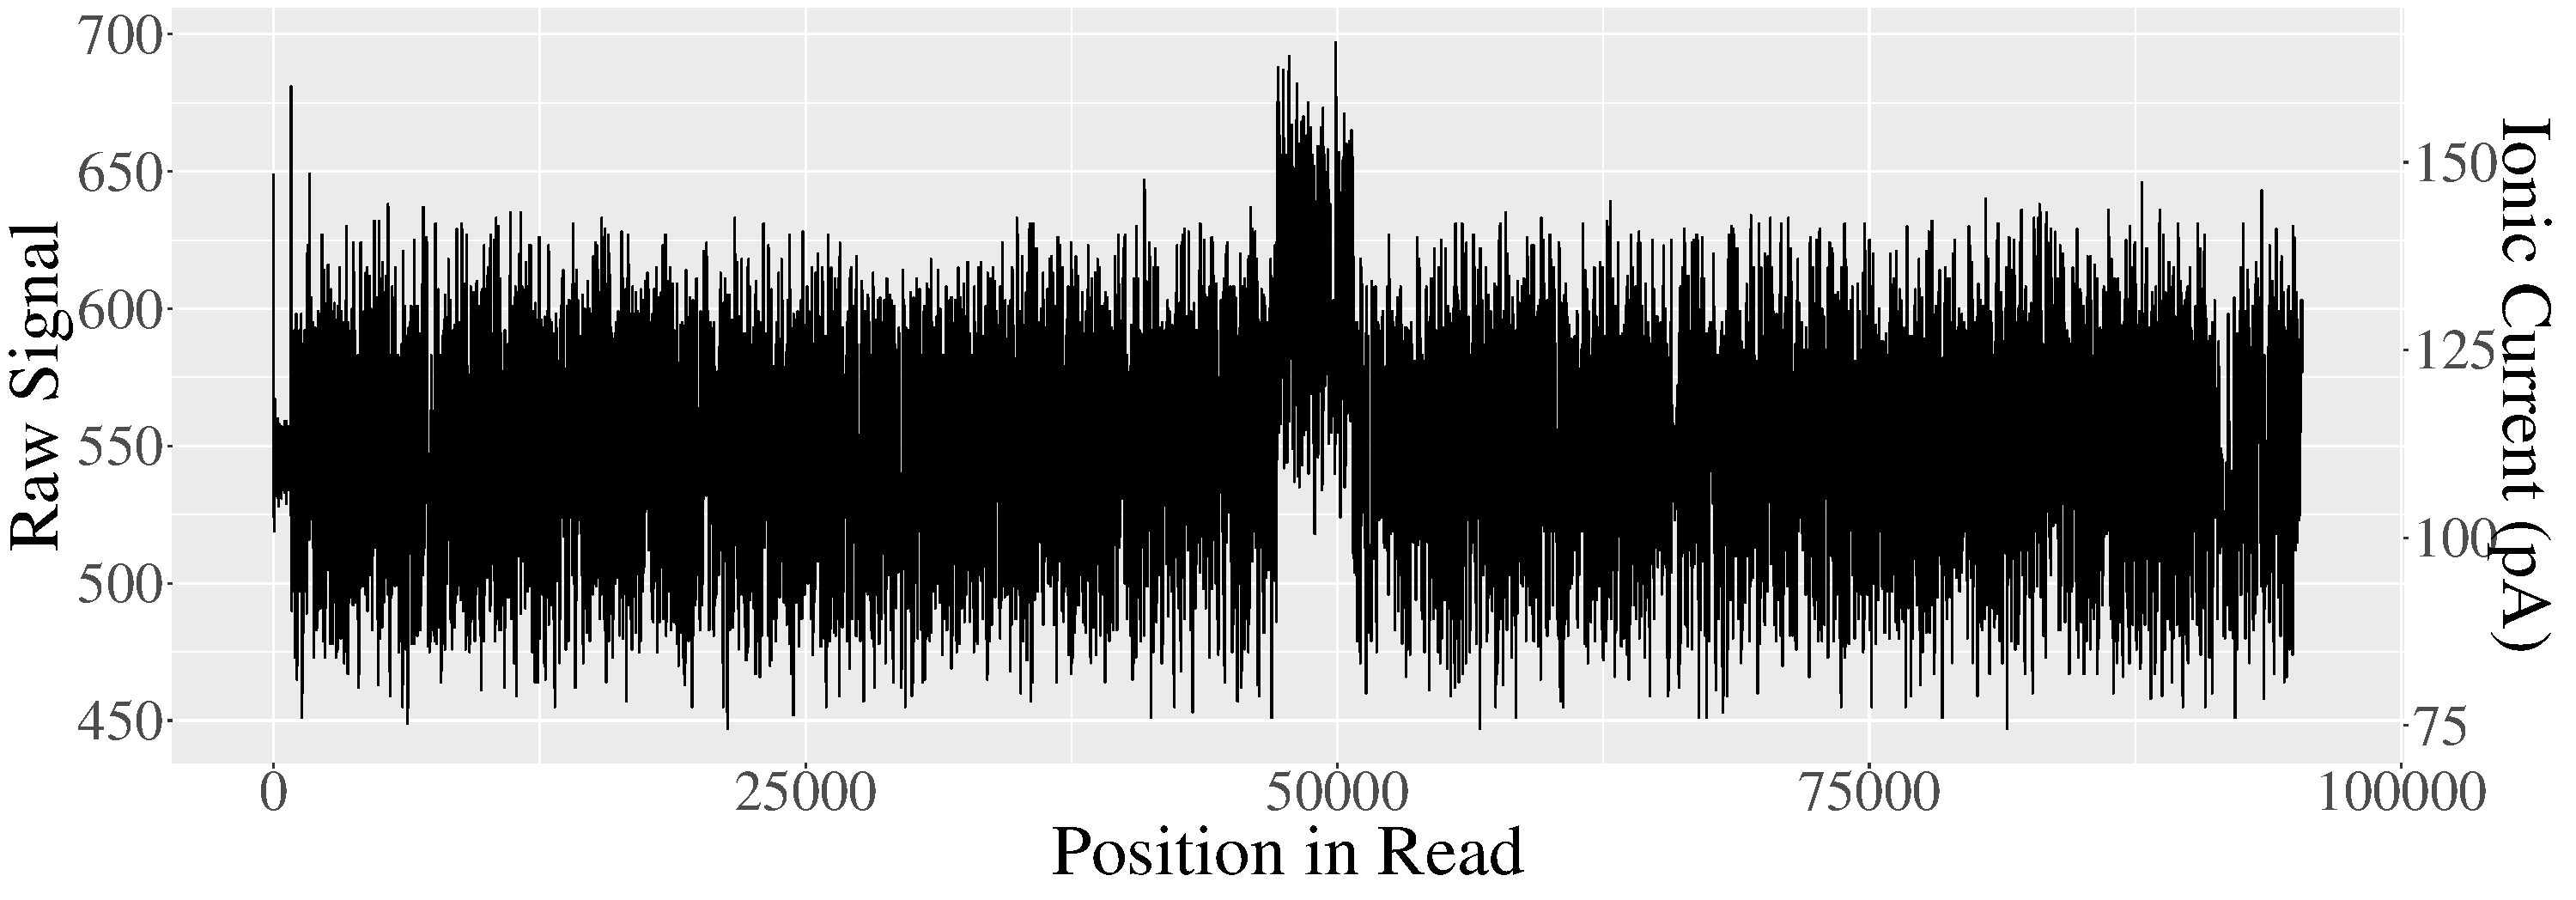
\includegraphics[scale=0.31]{plots/reads.e9f08690-171f-476f-9119-5330d0290126.raw.pa.pdf}
	\caption{\label{fig:read-e9f-pa}The read with ID e9f08690-171f-476f-9119-5330d0290126 from the NA12878 data set plotted against two axes. The primary $y$-axis (left) is the raw signal values and the secondary $y$-axis (right) is the ionic current found using equation \ref{eq:pa}. $535, 531, 529, 519, 535,\dots$ is the sequence starting from position 25000 and $106.73, 105.27, 104.54, 100.88, 106.73,\dots$ is the same sequence after converting to picoamperes (rounded to 2 decimal places).}
\end{figure}


The data consists of many sequences of unsigned integers known as \textit{reads} and their associated metadata. Each read represents the quantised ionic current measured across a nanopore as a single-stranded DNA or RNA molecule is driven through it. The current is typically recorded or `sampled' 4000 times a second by an electrode in the sensor chip and digitised using an analogue-to-digital converter (ADC). This recording frequency is known as the \textit{sampling rate} and is stored as metadata for each read. Disturbances in the ionic current caused by the molecule's biological structure can be used to determine its nucleic acid sequence.

Let each read (or `raw signal') be represented by
\[ x := (x_i\mid x_i \in \mathbb{Z} \cap [0, 2^{16})) \]
where $i\in \mathbb{Z}\cap [0, n)$. Computationally, $x$ is an unsigned 16-bit integer array with $n$ elements. However, in practice the full range of $2^{16}$ integers is never met; a property which will be further explored and heavily exploited. See Figure \ref{fig:read-e9f-pa} for an example of a read.

There are many metadata fields which are constant for all reads of the same sequencing run. This includes the sampling rate and every header attribute. Common header attributes include metadata relating to the ASIC chip such as its temperature at the start of the run, the ONT device being used, the start time of the run, its duration in minutes and whether DNA or RNA is being used \cite{slow5-spec}. See Table \ref{tab:data-meta}.

\begin{table}
    \caption{\label{tab:data-meta}The constant metadata of the NA12878 data set.}
    \begin{tabular}{|l|l|}%l|}
        \hline
	    Sampling Rate (Hz) & 4000\\
	ASIC Start Temperature (\textdegree C) & 31.996552\\
	Device Type & PromethION 48\\
	    Start Time (ISO 8601) & 2020-10-27T05:41:50Z\\
	    Duration (mins) & 4320\\
	    Experiment Type & DNA\\
	\hline
    \end{tabular}
\end{table}

\begin{table}
    \caption{\label{tab:data-read-meta}The variable metadata of the read with ID e9f08690-171f-476f-9119-5330d0290126 from the NA12878 data set.}
    \begin{tabular}{|l|l|}%l|}
        \hline
        %Read ID & e9f08690-171f-476f-9119-5330d0290126\\ %& 99671b17-feb4-492b-b119-77daf8e5794e \\
	Length & 95350\\ %& 155185 \\
	%Read & $649,565,541,535,535,\dots$\\ %& $434,419,416,411,426,\dots$\\
	%Digitisation & 2048\\
	Offset & -243\\
	%Range & 748.580139\\
	Channel No. & 2642\\ %& 109\\
	Pore No. & 4\\ %& 3 \\
	Channel Read Count & 437\\ %& 553\\
	Channel Data Point Count& 5599213\\ %& 7503934\\
    Median Before (pA) & 238.772018\\ %& 202.511917\\
	    End Reason & Signal Positive \\
	\hline
    \end{tabular}
\end{table}


The main read-variable metadata is the length $n$ and the information necessary for converting the read from quantised raw signal values into picoamperes (pA). This information is comprised of three fields: the digitisation, offset and range. The digitisation is the number of quantisation levels in the ADC which is typically 2048 ($2^{11}$) or 4096 ($2^{12}$). Each data point in a read is recorded using 16 bits; it is the closest multiple of a byte after 11 and 12 bits. The next field is the offset which is the ADC's offset error whilst the range is the sensor chip's full measurement range in picoamperes. To convert a raw signal value into picoamperes one does the following computation
\begin{equation}(raw + offset) \times \frac{range}{digitisation}. \label{eq:pa}\end{equation}
The digitisation and range fields are actually constant between reads since they are hardware-defined properties; it is the offset which varies among reads. See Table \ref{tab:data-read-meta}.

There are other read-variable metadata fields which are optionally included in the data but nonetheless may prove useful for a compression algorithm. These include the reason the read ended, flow cell location data comprised of the channel and pore number, the estimated median current level before the start of the read, and a count of the number of reads and data points previously recorded by the channel.

For the remainder of the thesis, the data which we will use for analysing the characteristics of nanopore signal data and for comparing compression methods is a downsampling of a typical human genome sequencing data set, generated from a reference sample known as NA12878. The NA12878 data set has been well studied and is used prolifically for benchmarking genomics tools. It originates from a Utah woman whose DNA reference was artificially recreated, treated using a short read eliminator kit and sequenced on an ONT PromethION 48 using two version R9.4.1 flow cells to obtain $\sim$30$\times$ coverage of her genome.
The data set was then downsampled a factor of $\sim$18 by obtaining the first \num{500000} reads.
%The data set was then downsampled a factor of $\sim$18 by obtaining the sequence of reads requested by a typical analysis application.
%More specifically, it was generated by sorting the reads by chromosome number and then base location to obtain a sorted order of reads by genomic coordinates.
%Downsampling produces a smaller representative data set which speeds up testing, and the results found should scale up to the whole data set.
The first reads usually contain more data than later reads as each nanopore deteriorates over its sequencing lifetime.
Downsampling produces a smaller data set which speeds up testing, and the compression results found will scale up to the whole data set.

It is highly likely that human DNA is the most commonly sequenced molecule of all sequencing technologies, as well as specifically of ONT devices.
Naturally then, most data sets that exist are the result of sequencing human DNA and hence share patterns inherit in human biology and the DNA sequencing process.
Hence, it makes sense to consider a human DNA data set in a study of data compression.
Furthermore, the PromethION flow cell produces the most yield out of all ONT flow cells so PromethION data is also highly suitable.
Thus, the NA12878 data set is a good choice for the comparison of nanopore signal compression methods.

The original data set contains \num{9083052} reads and consumes $\sim$2 TiB in raw binary or $\sim$707 GiB using VBZ compression. After downsampling, the data set contains \num{500000} reads and $\sim$57 billion data points, consuming $\sim$106 GiB in raw binary or $\sim$37 GiB when stored using VBZ. See Tables \ref{tab:data-orig} and \ref{tab:data} for an overview of the data sets. From now onwards, \textit{the data set} refers to the downsampling of the original NA12878 data set and can be downloaded from \url{https://slow5.page.link/na12878_prom_sub_slow5}.

\begin{table}
    \caption{\label{tab:data-orig}The original NA12878 data set.}
    \begin{tabular}{|l|l|}
        \hline
        Description & Adult Utah Female DNA\\
        \hline
	%Sequencer & ONT PromethION\\
	%Start time (ISO 8601) & 2020-10-27T05:41:50Z\\
	No. of reads & \num{9083052}\\
	%No. of data points ($\times 10^9$) & $\sim$ 57\\
	%Avg. read length & $\sim$ \num{113471}\\
	Size (BLOW5 none) &$\sim$ 2 TiB\\
	Size (BLOW5 VBZ) &  $\sim$ 707 GiB\\
	\hline
    \end{tabular}
\end{table}

\begin{table}
    \caption{\label{tab:data}The NA12878 data set.}
    \begin{tabular}{|l|l|}
        \hline
        Description & Adult Utah Female DNA\\
        \hline
	Sequencer & ONT PromethION\\
	Start time (ISO 8601) & 2020-10-27T05:41:50Z\\
	No. of reads & \num{500000}\\
	No. of signals ($\times 10^9$) & $\sim$ 57\\
	Avg. read length & $\sim$ \num{113471}\\
        \hline
	Gibibytes (in BLOW5 v0.2.0) & $\sim$ 39\\
	\hline
    \end{tabular}
\end{table}


The metadata accounts for lesser than 0.05\% of the raw binary data set's size, meaning that without storing any metadata the data set consumes roughly the same size. From a compression point of view there is much more to gain from focussing on compressing the read data. For this reason, future comparisons of file size including compression ratios will not represent the cost of storing metadata, only read data.

The raw signal values in the data set range from 158 to 1748 with a median of 474 and standard deviation of $\sim$ 35. See Table \ref{tab:rawsig}. The range is 1590 but the middle 99\% of the data ranges from 350 to 622. Figure \ref{fig:data-hist} shows the singular-width bin histogram of the raw signal values between 295 and 687.
As one can observe, the distribution is fairly symmetric around the centre with the median and mean very close to one another. However, it is slightly right-skewed with its right tail extending much further than its left. This is most evident by observing that the maximum is more than four times further from the median than the minimum is.
Most interestingly, the histogram is not smooth with the frequency of adjacent signal points varying drastically. For example, the value 455 occurs $\sim$6.3 times more often than 456.
In fact, on close inspection there is a cyclical pattern in the relative frequency of adjacent signal points in Figure \ref{fig:data-hist} which appears to repeats every 16 values. For example, consider the frequencies of values 456--471 and values 472--487.
%TODO put closeup figure showing pattern
This is most likely a result of the ADC unevenly digitising the analogue ionic current signal in some deterministic way.

\begin{table}
    \caption{\label{tab:rawsig} Summary statistics of the data's raw signal values.}
    \begin{tabular}{|l|l|}
        \hline
Min & 158\\
	    Q1 & 439\\

Q2 & 474\\
	    Q3 & 511\\
Max & 1748\\
\hline
Mean & 475.2245\\
	    Mode & 487\\
SD & 35.0675\\
	\hline
    \end{tabular}
\end{table}

\begin{figure}
	\centering
% Created by tikzDevice version 0.12.3.1 on 2022-09-19 10:24:26
% !TEX encoding = UTF-8 Unicode
\begin{tikzpicture}[x=1pt,y=1pt]
\definecolor{fillColor}{RGB}{255,255,255}
\path[use as bounding box,fill=fillColor,fill opacity=0.00] (0,0) rectangle (361.35,361.35);
\begin{scope}
\path[clip] (  0.00,  0.00) rectangle (361.35,361.35);
\definecolor{drawColor}{RGB}{255,255,255}
\definecolor{fillColor}{RGB}{255,255,255}

\path[draw=drawColor,line width= 0.6pt,line join=round,line cap=round,fill=fillColor] (  0.00,  0.00) rectangle (361.35,361.35);
\end{scope}
\begin{scope}
\path[clip] ( 36.11, 30.69) rectangle (355.85,355.85);
\definecolor{fillColor}{gray}{0.92}

\path[fill=fillColor] ( 36.11, 30.69) rectangle (355.85,355.85);
\definecolor{drawColor}{RGB}{255,255,255}

\path[draw=drawColor,line width= 0.3pt,line join=round] ( 36.11, 81.60) --
	(355.85, 81.60);

\path[draw=drawColor,line width= 0.3pt,line join=round] ( 36.11,153.87) --
	(355.85,153.87);

\path[draw=drawColor,line width= 0.3pt,line join=round] ( 36.11,226.14) --
	(355.85,226.14);

\path[draw=drawColor,line width= 0.3pt,line join=round] ( 36.11,298.41) --
	(355.85,298.41);

\path[draw=drawColor,line width= 0.3pt,line join=round] ( 91.43, 30.69) --
	( 91.43,355.85);

\path[draw=drawColor,line width= 0.3pt,line join=round] (165.58, 30.69) --
	(165.58,355.85);

\path[draw=drawColor,line width= 0.3pt,line join=round] (239.73, 30.69) --
	(239.73,355.85);

\path[draw=drawColor,line width= 0.3pt,line join=round] (313.88, 30.69) --
	(313.88,355.85);

\path[draw=drawColor,line width= 0.6pt,line join=round] ( 36.11, 45.47) --
	(355.85, 45.47);

\path[draw=drawColor,line width= 0.6pt,line join=round] ( 36.11,117.73) --
	(355.85,117.73);

\path[draw=drawColor,line width= 0.6pt,line join=round] ( 36.11,190.00) --
	(355.85,190.00);

\path[draw=drawColor,line width= 0.6pt,line join=round] ( 36.11,262.27) --
	(355.85,262.27);

\path[draw=drawColor,line width= 0.6pt,line join=round] ( 36.11,334.54) --
	(355.85,334.54);

\path[draw=drawColor,line width= 0.6pt,line join=round] ( 54.35, 30.69) --
	( 54.35,355.85);

\path[draw=drawColor,line width= 0.6pt,line join=round] (128.50, 30.69) --
	(128.50,355.85);

\path[draw=drawColor,line width= 0.6pt,line join=round] (202.65, 30.69) --
	(202.65,355.85);

\path[draw=drawColor,line width= 0.6pt,line join=round] (276.81, 30.69) --
	(276.81,355.85);

\path[draw=drawColor,line width= 0.6pt,line join=round] (350.96, 30.69) --
	(350.96,355.85);
\definecolor{fillColor}{gray}{0.35}

\path[fill=fillColor] ( 51.05, 45.47) rectangle ( 51.72, 45.53);

\path[fill=fillColor] ( 51.79, 45.47) rectangle ( 52.46, 45.66);

\path[fill=fillColor] ( 52.54, 45.47) rectangle ( 53.20, 45.64);

\path[fill=fillColor] ( 53.28, 45.47) rectangle ( 53.94, 45.72);

\path[fill=fillColor] ( 54.02, 45.47) rectangle ( 54.69, 45.69);

\path[fill=fillColor] ( 54.76, 45.47) rectangle ( 55.43, 45.65);

\path[fill=fillColor] ( 55.50, 45.47) rectangle ( 56.17, 45.71);

\path[fill=fillColor] ( 56.24, 45.47) rectangle ( 56.91, 45.80);

\path[fill=fillColor] ( 56.98, 45.47) rectangle ( 57.65, 45.79);

\path[fill=fillColor] ( 57.73, 45.47) rectangle ( 58.39, 45.75);

\path[fill=fillColor] ( 58.47, 45.47) rectangle ( 59.14, 45.71);

\path[fill=fillColor] ( 59.21, 45.47) rectangle ( 59.88, 45.88);

\path[fill=fillColor] ( 59.95, 45.47) rectangle ( 60.62, 45.70);

\path[fill=fillColor] ( 60.69, 45.47) rectangle ( 61.36, 45.76);

\path[fill=fillColor] ( 61.43, 45.47) rectangle ( 62.10, 45.80);

\path[fill=fillColor] ( 62.18, 45.47) rectangle ( 62.84, 46.10);

\path[fill=fillColor] ( 62.92, 45.47) rectangle ( 63.58, 45.69);

\path[fill=fillColor] ( 63.66, 45.47) rectangle ( 64.33, 45.90);

\path[fill=fillColor] ( 64.40, 45.47) rectangle ( 65.07, 45.83);

\path[fill=fillColor] ( 65.14, 45.47) rectangle ( 65.81, 46.01);

\path[fill=fillColor] ( 65.88, 45.47) rectangle ( 66.55, 45.99);

\path[fill=fillColor] ( 66.62, 45.47) rectangle ( 67.29, 45.92);

\path[fill=fillColor] ( 67.37, 45.47) rectangle ( 68.03, 46.06);

\path[fill=fillColor] ( 68.11, 45.47) rectangle ( 68.77, 46.40);

\path[fill=fillColor] ( 68.85, 45.47) rectangle ( 69.52, 46.28);

\path[fill=fillColor] ( 69.59, 45.47) rectangle ( 70.26, 46.26);

\path[fill=fillColor] ( 70.33, 45.47) rectangle ( 71.00, 46.19);

\path[fill=fillColor] ( 71.07, 45.47) rectangle ( 71.74, 46.62);

\path[fill=fillColor] ( 71.81, 45.47) rectangle ( 72.48, 46.25);

\path[fill=fillColor] ( 72.56, 45.47) rectangle ( 73.22, 46.38);

\path[fill=fillColor] ( 73.30, 45.47) rectangle ( 73.97, 46.55);

\path[fill=fillColor] ( 74.04, 45.47) rectangle ( 74.71, 47.78);

\path[fill=fillColor] ( 74.78, 45.47) rectangle ( 75.45, 45.99);

\path[fill=fillColor] ( 75.52, 45.47) rectangle ( 76.19, 46.82);

\path[fill=fillColor] ( 76.26, 45.47) rectangle ( 76.93, 46.72);

\path[fill=fillColor] ( 77.01, 45.47) rectangle ( 77.67, 47.31);

\path[fill=fillColor] ( 77.75, 45.47) rectangle ( 78.41, 47.27);

\path[fill=fillColor] ( 78.49, 45.47) rectangle ( 79.16, 47.05);

\path[fill=fillColor] ( 79.23, 45.47) rectangle ( 79.90, 47.59);

\path[fill=fillColor] ( 79.97, 45.47) rectangle ( 80.64, 48.70);

\path[fill=fillColor] ( 80.71, 45.47) rectangle ( 81.38, 48.39);

\path[fill=fillColor] ( 81.45, 45.47) rectangle ( 82.12, 48.37);

\path[fill=fillColor] ( 82.20, 45.47) rectangle ( 82.86, 48.01);

\path[fill=fillColor] ( 82.94, 45.47) rectangle ( 83.60, 49.59);

\path[fill=fillColor] ( 83.68, 45.47) rectangle ( 84.35, 48.22);

\path[fill=fillColor] ( 84.42, 45.47) rectangle ( 85.09, 48.75);

\path[fill=fillColor] ( 85.16, 45.47) rectangle ( 85.83, 49.25);

\path[fill=fillColor] ( 85.90, 45.47) rectangle ( 86.57, 52.42);

\path[fill=fillColor] ( 86.65, 45.47) rectangle ( 87.31, 48.00);

\path[fill=fillColor] ( 87.39, 45.47) rectangle ( 88.05, 50.43);

\path[fill=fillColor] ( 88.13, 45.47) rectangle ( 88.80, 49.56);

\path[fill=fillColor] ( 88.87, 45.47) rectangle ( 89.54, 51.51);

\path[fill=fillColor] ( 89.61, 45.47) rectangle ( 90.28, 51.28);

\path[fill=fillColor] ( 90.35, 45.47) rectangle ( 91.02, 50.52);

\path[fill=fillColor] ( 91.09, 45.47) rectangle ( 91.76, 52.07);

\path[fill=fillColor] ( 91.84, 45.47) rectangle ( 92.50, 54.53);

\path[fill=fillColor] ( 92.58, 45.47) rectangle ( 93.24, 55.33);

\path[fill=fillColor] ( 93.32, 45.47) rectangle ( 93.99, 54.12);

\path[fill=fillColor] ( 94.06, 45.47) rectangle ( 94.73, 53.02);

\path[fill=fillColor] ( 94.80, 45.47) rectangle ( 95.47, 57.88);

\path[fill=fillColor] ( 95.54, 45.47) rectangle ( 96.21, 53.16);

\path[fill=fillColor] ( 96.28, 45.47) rectangle ( 96.95, 54.86);

\path[fill=fillColor] ( 97.03, 45.47) rectangle ( 97.69, 56.14);

\path[fill=fillColor] ( 97.77, 45.47) rectangle ( 98.44, 68.59);

\path[fill=fillColor] ( 98.51, 45.47) rectangle ( 99.18, 49.85);

\path[fill=fillColor] ( 99.25, 45.47) rectangle ( 99.92, 57.84);

\path[fill=fillColor] ( 99.99, 45.47) rectangle (100.66, 56.51);

\path[fill=fillColor] (100.73, 45.47) rectangle (101.40, 61.93);

\path[fill=fillColor] (101.48, 45.47) rectangle (102.14, 60.27);

\path[fill=fillColor] (102.22, 45.47) rectangle (102.88, 58.38);

\path[fill=fillColor] (102.96, 45.47) rectangle (103.63, 62.08);

\path[fill=fillColor] (103.70, 45.47) rectangle (104.37, 70.01);

\path[fill=fillColor] (104.44, 45.47) rectangle (105.11, 67.13);

\path[fill=fillColor] (105.18, 45.47) rectangle (105.85, 66.29);

\path[fill=fillColor] (105.92, 45.47) rectangle (106.59, 62.77);

\path[fill=fillColor] (106.67, 45.47) rectangle (107.33, 74.50);

\path[fill=fillColor] (107.41, 45.47) rectangle (108.07, 62.37);

\path[fill=fillColor] (108.15, 45.47) rectangle (108.82, 66.45);

\path[fill=fillColor] (108.89, 45.47) rectangle (109.56, 68.66);

\path[fill=fillColor] (109.63, 45.47) rectangle (110.30, 88.95);

\path[fill=fillColor] (110.37, 45.47) rectangle (111.04, 59.40);

\path[fill=fillColor] (111.11, 45.47) rectangle (111.78, 74.03);

\path[fill=fillColor] (111.86, 45.47) rectangle (112.52, 67.97);

\path[fill=fillColor] (112.60, 45.47) rectangle (113.27, 79.49);

\path[fill=fillColor] (113.34, 45.47) rectangle (114.01, 75.93);

\path[fill=fillColor] (114.08, 45.47) rectangle (114.75, 71.63);

\path[fill=fillColor] (114.82, 45.47) rectangle (115.49, 78.62);

\path[fill=fillColor] (115.56, 45.47) rectangle (116.23,135.08);

\path[fill=fillColor] (116.31, 45.47) rectangle (116.97, 54.11);

\path[fill=fillColor] (117.05, 45.47) rectangle (117.71, 75.70);

\path[fill=fillColor] (117.79, 45.47) rectangle (118.46, 79.05);

\path[fill=fillColor] (118.53, 45.47) rectangle (119.20, 99.15);

\path[fill=fillColor] (119.27, 45.47) rectangle (119.94, 78.20);

\path[fill=fillColor] (120.01, 45.47) rectangle (120.68, 83.67);

\path[fill=fillColor] (120.75, 45.47) rectangle (121.42, 88.49);

\path[fill=fillColor] (121.50, 45.47) rectangle (122.16,133.84);

\path[fill=fillColor] (122.24, 45.47) rectangle (122.90, 63.33);

\path[fill=fillColor] (122.98, 45.47) rectangle (123.65, 91.15);

\path[fill=fillColor] (123.72, 45.47) rectangle (124.39, 86.16);

\path[fill=fillColor] (124.46, 45.47) rectangle (125.13,104.13);

\path[fill=fillColor] (125.20, 45.47) rectangle (125.87, 98.07);

\path[fill=fillColor] (125.95, 45.47) rectangle (126.61, 89.47);

\path[fill=fillColor] (126.69, 45.47) rectangle (127.35,101.74);

\path[fill=fillColor] (127.43, 45.47) rectangle (128.10,126.65);

\path[fill=fillColor] (128.17, 45.47) rectangle (128.84,115.37);

\path[fill=fillColor] (128.91, 45.47) rectangle (129.58,110.28);

\path[fill=fillColor] (129.65, 45.47) rectangle (130.32, 99.28);

\path[fill=fillColor] (130.39, 45.47) rectangle (131.06,133.47);

\path[fill=fillColor] (131.14, 45.47) rectangle (131.80, 96.00);

\path[fill=fillColor] (131.88, 45.47) rectangle (132.54,105.80);

\path[fill=fillColor] (132.62, 45.47) rectangle (133.29,111.94);

\path[fill=fillColor] (133.36, 45.47) rectangle (134.03,164.97);

\path[fill=fillColor] (134.10, 45.47) rectangle (134.77, 85.65);

\path[fill=fillColor] (134.84, 45.47) rectangle (135.51,121.61);

\path[fill=fillColor] (135.58, 45.47) rectangle (136.25,105.35);

\path[fill=fillColor] (136.33, 45.47) rectangle (136.99,133.30);

\path[fill=fillColor] (137.07, 45.47) rectangle (137.74,124.36);

\path[fill=fillColor] (137.81, 45.47) rectangle (138.48,110.32);

\path[fill=fillColor] (138.55, 45.47) rectangle (139.22,127.37);

\path[fill=fillColor] (139.29, 45.47) rectangle (139.96,163.46);

\path[fill=fillColor] (140.03, 45.47) rectangle (140.70,148.19);

\path[fill=fillColor] (140.78, 45.47) rectangle (141.44,137.58);

\path[fill=fillColor] (141.52, 45.47) rectangle (142.18,122.15);

\path[fill=fillColor] (142.26, 45.47) rectangle (142.93,173.21);

\path[fill=fillColor] (143.00, 45.47) rectangle (143.67,114.39);

\path[fill=fillColor] (143.74, 45.47) rectangle (144.41,129.26);

\path[fill=fillColor] (144.48, 45.47) rectangle (145.15,137.31);

\path[fill=fillColor] (145.22, 45.47) rectangle (145.89,240.76);

\path[fill=fillColor] (145.97, 45.47) rectangle (146.63, 80.01);

\path[fill=fillColor] (146.71, 45.47) rectangle (147.37,139.16);

\path[fill=fillColor] (147.45, 45.47) rectangle (148.12,126.64);

\path[fill=fillColor] (148.19, 45.47) rectangle (148.86,167.15);

\path[fill=fillColor] (148.93, 45.47) rectangle (149.60,149.44);

\path[fill=fillColor] (149.67, 45.47) rectangle (150.34,131.32);

\path[fill=fillColor] (150.41, 45.47) rectangle (151.08,153.71);

\path[fill=fillColor] (151.16, 45.47) rectangle (151.82,199.18);

\path[fill=fillColor] (151.90, 45.47) rectangle (152.57,181.51);

\path[fill=fillColor] (152.64, 45.47) rectangle (153.31,167.09);

\path[fill=fillColor] (153.38, 45.47) rectangle (154.05,142.01);

\path[fill=fillColor] (154.12, 45.47) rectangle (154.79,211.90);

\path[fill=fillColor] (154.86, 45.47) rectangle (155.53,131.59);

\path[fill=fillColor] (155.61, 45.47) rectangle (156.27,151.91);

\path[fill=fillColor] (156.35, 45.47) rectangle (157.01,160.29);

\path[fill=fillColor] (157.09, 45.47) rectangle (157.76,257.39);

\path[fill=fillColor] (157.83, 45.47) rectangle (158.50,111.83);

\path[fill=fillColor] (158.57, 45.47) rectangle (159.24,175.08);

\path[fill=fillColor] (159.31, 45.47) rectangle (159.98,143.03);

\path[fill=fillColor] (160.05, 45.47) rectangle (160.72,194.08);

\path[fill=fillColor] (160.80, 45.47) rectangle (161.46,174.21);

\path[fill=fillColor] (161.54, 45.47) rectangle (162.20,149.77);

\path[fill=fillColor] (162.28, 45.47) rectangle (162.95,175.60);

\path[fill=fillColor] (163.02, 45.47) rectangle (163.69,254.37);

\path[fill=fillColor] (163.76, 45.47) rectangle (164.43,186.26);

\path[fill=fillColor] (164.50, 45.47) rectangle (165.17,187.93);

\path[fill=fillColor] (165.25, 45.47) rectangle (165.91,160.33);

\path[fill=fillColor] (165.99, 45.47) rectangle (166.65,241.64);

\path[fill=fillColor] (166.73, 45.47) rectangle (167.40,146.40);

\path[fill=fillColor] (167.47, 45.47) rectangle (168.14,168.14);

\path[fill=fillColor] (168.21, 45.47) rectangle (168.88,178.30);

\path[fill=fillColor] (168.95, 45.47) rectangle (169.62,334.23);

\path[fill=fillColor] (169.69, 45.47) rectangle (170.36, 91.26);

\path[fill=fillColor] (170.44, 45.47) rectangle (171.10,176.09);

\path[fill=fillColor] (171.18, 45.47) rectangle (171.84,156.13);

\path[fill=fillColor] (171.92, 45.47) rectangle (172.59,215.23);

\path[fill=fillColor] (172.66, 45.47) rectangle (173.33,187.91);

\path[fill=fillColor] (173.40, 45.47) rectangle (174.07,160.40);

\path[fill=fillColor] (174.14, 45.47) rectangle (174.81,189.26);

\path[fill=fillColor] (174.88, 45.47) rectangle (175.55,256.67);

\path[fill=fillColor] (175.63, 45.47) rectangle (176.29,216.88);

\path[fill=fillColor] (176.37, 45.47) rectangle (177.04,202.71);

\path[fill=fillColor] (177.11, 45.47) rectangle (177.78,166.03);

\path[fill=fillColor] (177.85, 45.47) rectangle (178.52,258.56);

\path[fill=fillColor] (178.59, 45.47) rectangle (179.26,151.03);

\path[fill=fillColor] (179.33, 45.47) rectangle (180.00,175.36);

\path[fill=fillColor] (180.08, 45.47) rectangle (180.74,184.25);

\path[fill=fillColor] (180.82, 45.47) rectangle (181.48,304.67);

\path[fill=fillColor] (181.56, 45.47) rectangle (182.23,122.72);

\path[fill=fillColor] (182.30, 45.47) rectangle (182.97,198.20);

\path[fill=fillColor] (183.04, 45.47) rectangle (183.71,156.32);

\path[fill=fillColor] (183.78, 45.47) rectangle (184.45,217.62);

\path[fill=fillColor] (184.52, 45.47) rectangle (185.19,193.02);

\path[fill=fillColor] (185.27, 45.47) rectangle (185.93,161.40);

\path[fill=fillColor] (186.01, 45.47) rectangle (186.67,189.34);

\path[fill=fillColor] (186.75, 45.47) rectangle (187.42,253.05);

\path[fill=fillColor] (187.49, 45.47) rectangle (188.16,223.56);

\path[fill=fillColor] (188.23, 45.47) rectangle (188.90,199.76);

\path[fill=fillColor] (188.97, 45.47) rectangle (189.64,163.73);

\path[fill=fillColor] (189.71, 45.47) rectangle (190.38,258.86);

\path[fill=fillColor] (190.46, 45.47) rectangle (191.12,144.96);

\path[fill=fillColor] (191.20, 45.47) rectangle (191.87,170.12);

\path[fill=fillColor] (191.94, 45.47) rectangle (192.61,178.35);

\path[fill=fillColor] (192.68, 45.47) rectangle (193.35,341.07);

\path[fill=fillColor] (193.42, 45.47) rectangle (194.09, 88.36);

\path[fill=fillColor] (194.16, 45.47) rectangle (194.83,173.31);

\path[fill=fillColor] (194.91, 45.47) rectangle (195.57,149.64);

\path[fill=fillColor] (195.65, 45.47) rectangle (196.31,211.61);

\path[fill=fillColor] (196.39, 45.47) rectangle (197.06,180.78);

\path[fill=fillColor] (197.13, 45.47) rectangle (197.80,152.35);

\path[fill=fillColor] (197.87, 45.47) rectangle (198.54,178.14);

\path[fill=fillColor] (198.61, 45.47) rectangle (199.28,234.09);

\path[fill=fillColor] (199.35, 45.47) rectangle (200.02,210.38);

\path[fill=fillColor] (200.10, 45.47) rectangle (200.76,188.10);

\path[fill=fillColor] (200.84, 45.47) rectangle (201.50,149.59);

\path[fill=fillColor] (201.58, 45.47) rectangle (202.25,239.72);

\path[fill=fillColor] (202.32, 45.47) rectangle (202.99,133.34);

\path[fill=fillColor] (203.06, 45.47) rectangle (203.73,156.48);

\path[fill=fillColor] (203.80, 45.47) rectangle (204.47,162.53);

\path[fill=fillColor] (204.55, 45.47) rectangle (205.21,267.80);

\path[fill=fillColor] (205.29, 45.47) rectangle (205.95,109.31);

\path[fill=fillColor] (206.03, 45.47) rectangle (206.70,173.18);

\path[fill=fillColor] (206.77, 45.47) rectangle (207.44,133.53);

\path[fill=fillColor] (207.51, 45.47) rectangle (208.18,187.81);

\path[fill=fillColor] (208.25, 45.47) rectangle (208.92,164.45);

\path[fill=fillColor] (208.99, 45.47) rectangle (209.66,137.06);

\path[fill=fillColor] (209.74, 45.47) rectangle (210.40,157.80);

\path[fill=fillColor] (210.48, 45.47) rectangle (211.14,180.99);

\path[fill=fillColor] (211.22, 45.47) rectangle (211.89,198.58);

\path[fill=fillColor] (211.96, 45.47) rectangle (212.63,162.15);

\path[fill=fillColor] (212.70, 45.47) rectangle (213.37,135.28);

\path[fill=fillColor] (213.44, 45.47) rectangle (214.11,201.77);

\path[fill=fillColor] (214.18, 45.47) rectangle (214.85,123.84);

\path[fill=fillColor] (214.93, 45.47) rectangle (215.59,135.12);

\path[fill=fillColor] (215.67, 45.47) rectangle (216.34,143.70);

\path[fill=fillColor] (216.41, 45.47) rectangle (217.08,248.59);

\path[fill=fillColor] (217.15, 45.47) rectangle (217.82, 82.28);

\path[fill=fillColor] (217.89, 45.47) rectangle (218.56,138.27);

\path[fill=fillColor] (218.63, 45.47) rectangle (219.30,118.76);

\path[fill=fillColor] (219.38, 45.47) rectangle (220.04,157.22);

\path[fill=fillColor] (220.12, 45.47) rectangle (220.78,142.78);

\path[fill=fillColor] (220.86, 45.47) rectangle (221.53,116.77);

\path[fill=fillColor] (221.60, 45.47) rectangle (222.27,135.82);

\path[fill=fillColor] (222.34, 45.47) rectangle (223.01,170.53);

\path[fill=fillColor] (223.08, 45.47) rectangle (223.75,155.96);

\path[fill=fillColor] (223.82, 45.47) rectangle (224.49,137.45);

\path[fill=fillColor] (224.57, 45.47) rectangle (225.23,112.77);

\path[fill=fillColor] (225.31, 45.47) rectangle (225.97,167.15);

\path[fill=fillColor] (226.05, 45.47) rectangle (226.72,104.37);

\path[fill=fillColor] (226.79, 45.47) rectangle (227.46,113.79);

\path[fill=fillColor] (227.53, 45.47) rectangle (228.20,119.46);

\path[fill=fillColor] (228.27, 45.47) rectangle (228.94,176.54);

\path[fill=fillColor] (229.01, 45.47) rectangle (229.68, 89.95);

\path[fill=fillColor] (229.76, 45.47) rectangle (230.42,122.88);

\path[fill=fillColor] (230.50, 45.47) rectangle (231.17, 98.54);

\path[fill=fillColor] (231.24, 45.47) rectangle (231.91,127.73);

\path[fill=fillColor] (231.98, 45.47) rectangle (232.65,118.61);

\path[fill=fillColor] (232.72, 45.47) rectangle (233.39, 97.89);

\path[fill=fillColor] (233.46, 45.47) rectangle (234.13,111.36);

\path[fill=fillColor] (234.21, 45.47) rectangle (234.87,139.57);

\path[fill=fillColor] (234.95, 45.47) rectangle (235.61,124.40);

\path[fill=fillColor] (235.69, 45.47) rectangle (236.36,111.29);

\path[fill=fillColor] (236.43, 45.47) rectangle (237.10, 93.71);

\path[fill=fillColor] (237.17, 45.47) rectangle (237.84,133.82);

\path[fill=fillColor] (237.91, 45.47) rectangle (238.58, 86.25);

\path[fill=fillColor] (238.65, 45.47) rectangle (239.32, 93.32);

\path[fill=fillColor] (239.40, 45.47) rectangle (240.06, 97.23);

\path[fill=fillColor] (240.14, 45.47) rectangle (240.80,153.65);

\path[fill=fillColor] (240.88, 45.47) rectangle (241.55, 64.06);

\path[fill=fillColor] (241.62, 45.47) rectangle (242.29, 93.74);

\path[fill=fillColor] (242.36, 45.47) rectangle (243.03, 81.86);

\path[fill=fillColor] (243.10, 45.47) rectangle (243.77,102.75);

\path[fill=fillColor] (243.85, 45.47) rectangle (244.51, 94.05);

\path[fill=fillColor] (244.59, 45.47) rectangle (245.25, 80.49);

\path[fill=fillColor] (245.33, 45.47) rectangle (246.00, 89.36);

\path[fill=fillColor] (246.07, 45.47) rectangle (246.74,103.28);

\path[fill=fillColor] (246.81, 45.47) rectangle (247.48,101.45);

\path[fill=fillColor] (247.55, 45.47) rectangle (248.22, 89.00);

\path[fill=fillColor] (248.29, 45.47) rectangle (248.96, 75.95);

\path[fill=fillColor] (249.04, 45.47) rectangle (249.70,102.58);

\path[fill=fillColor] (249.78, 45.47) rectangle (250.44, 71.25);

\path[fill=fillColor] (250.52, 45.47) rectangle (251.19, 75.86);

\path[fill=fillColor] (251.26, 45.47) rectangle (251.93, 77.94);

\path[fill=fillColor] (252.00, 45.47) rectangle (252.67,102.76);

\path[fill=fillColor] (252.74, 45.47) rectangle (253.41, 64.79);

\path[fill=fillColor] (253.48, 45.47) rectangle (254.15, 78.69);

\path[fill=fillColor] (254.23, 45.47) rectangle (254.89, 67.34);

\path[fill=fillColor] (254.97, 45.47) rectangle (255.64, 80.10);

\path[fill=fillColor] (255.71, 45.47) rectangle (256.38, 75.49);

\path[fill=fillColor] (256.45, 45.47) rectangle (257.12, 66.71);

\path[fill=fillColor] (257.19, 45.47) rectangle (257.86, 71.82);

\path[fill=fillColor] (257.93, 45.47) rectangle (258.60, 86.17);

\path[fill=fillColor] (258.68, 45.47) rectangle (259.34, 73.06);

\path[fill=fillColor] (259.42, 45.47) rectangle (260.08, 70.86);

\path[fill=fillColor] (260.16, 45.47) rectangle (260.83, 63.66);

\path[fill=fillColor] (260.90, 45.47) rectangle (261.57, 78.67);

\path[fill=fillColor] (261.64, 45.47) rectangle (262.31, 60.75);

\path[fill=fillColor] (262.38, 45.47) rectangle (263.05, 63.01);

\path[fill=fillColor] (263.12, 45.47) rectangle (263.79, 64.32);

\path[fill=fillColor] (263.87, 45.47) rectangle (264.53, 84.13);

\path[fill=fillColor] (264.61, 45.47) rectangle (265.27, 52.13);

\path[fill=fillColor] (265.35, 45.47) rectangle (266.02, 62.54);

\path[fill=fillColor] (266.09, 45.47) rectangle (266.76, 58.03);

\path[fill=fillColor] (266.83, 45.47) rectangle (267.50, 65.13);

\path[fill=fillColor] (267.57, 45.47) rectangle (268.24, 62.08);

\path[fill=fillColor] (268.31, 45.47) rectangle (268.98, 57.30);

\path[fill=fillColor] (269.06, 45.47) rectangle (269.72, 60.10);

\path[fill=fillColor] (269.80, 45.47) rectangle (270.47, 66.11);

\path[fill=fillColor] (270.54, 45.47) rectangle (271.21, 62.16);

\path[fill=fillColor] (271.28, 45.47) rectangle (271.95, 59.49);

\path[fill=fillColor] (272.02, 45.47) rectangle (272.69, 55.17);

\path[fill=fillColor] (272.76, 45.47) rectangle (273.43, 63.34);

\path[fill=fillColor] (273.51, 45.47) rectangle (274.17, 53.68);

\path[fill=fillColor] (274.25, 45.47) rectangle (274.91, 54.91);

\path[fill=fillColor] (274.99, 45.47) rectangle (275.66, 55.50);

\path[fill=fillColor] (275.73, 45.47) rectangle (276.40, 62.73);

\path[fill=fillColor] (276.47, 45.47) rectangle (277.14, 51.45);

\path[fill=fillColor] (277.21, 45.47) rectangle (277.88, 55.45);

\path[fill=fillColor] (277.95, 45.47) rectangle (278.62, 52.00);

\path[fill=fillColor] (278.70, 45.47) rectangle (279.36, 55.64);

\path[fill=fillColor] (279.44, 45.47) rectangle (280.10, 54.29);

\path[fill=fillColor] (280.18, 45.47) rectangle (280.85, 51.70);

\path[fill=fillColor] (280.92, 45.47) rectangle (281.59, 53.08);

\path[fill=fillColor] (281.66, 45.47) rectangle (282.33, 55.79);

\path[fill=fillColor] (282.40, 45.47) rectangle (283.07, 54.67);

\path[fill=fillColor] (283.15, 45.47) rectangle (283.81, 52.66);

\path[fill=fillColor] (283.89, 45.47) rectangle (284.55, 50.55);

\path[fill=fillColor] (284.63, 45.47) rectangle (285.30, 54.72);

\path[fill=fillColor] (285.37, 45.47) rectangle (286.04, 49.67);

\path[fill=fillColor] (286.11, 45.47) rectangle (286.78, 50.33);

\path[fill=fillColor] (286.85, 45.47) rectangle (287.52, 50.64);

\path[fill=fillColor] (287.59, 45.47) rectangle (288.26, 55.81);

\path[fill=fillColor] (288.34, 45.47) rectangle (289.00, 47.38);

\path[fill=fillColor] (289.08, 45.47) rectangle (289.74, 50.16);

\path[fill=fillColor] (289.82, 45.47) rectangle (290.49, 48.88);

\path[fill=fillColor] (290.56, 45.47) rectangle (291.23, 50.77);

\path[fill=fillColor] (291.30, 45.47) rectangle (291.97, 49.90);

\path[fill=fillColor] (292.04, 45.47) rectangle (292.71, 48.68);

\path[fill=fillColor] (292.78, 45.47) rectangle (293.45, 49.38);

\path[fill=fillColor] (293.53, 45.47) rectangle (294.19, 50.66);

\path[fill=fillColor] (294.27, 45.47) rectangle (294.94, 50.20);

\path[fill=fillColor] (295.01, 45.47) rectangle (295.68, 49.20);

\path[fill=fillColor] (295.75, 45.47) rectangle (296.42, 48.06);

\path[fill=fillColor] (296.49, 45.47) rectangle (297.16, 50.20);

\path[fill=fillColor] (297.23, 45.47) rectangle (297.90, 47.66);

\path[fill=fillColor] (297.98, 45.47) rectangle (298.64, 48.00);

\path[fill=fillColor] (298.72, 45.47) rectangle (299.38, 48.15);

\path[fill=fillColor] (299.46, 45.47) rectangle (300.13, 50.00);

\path[fill=fillColor] (300.20, 45.47) rectangle (300.87, 47.12);

\path[fill=fillColor] (300.94, 45.47) rectangle (301.61, 48.16);

\path[fill=fillColor] (301.68, 45.47) rectangle (302.35, 47.24);

\path[fill=fillColor] (302.42, 45.47) rectangle (303.09, 48.21);

\path[fill=fillColor] (303.17, 45.47) rectangle (303.83, 47.84);

\path[fill=fillColor] (303.91, 45.47) rectangle (304.57, 47.19);

\path[fill=fillColor] (304.65, 45.47) rectangle (305.32, 47.54);

\path[fill=fillColor] (305.39, 45.47) rectangle (306.06, 48.13);

\path[fill=fillColor] (306.13, 45.47) rectangle (306.80, 48.23);

\path[fill=fillColor] (306.87, 45.47) rectangle (307.54, 47.44);

\path[fill=fillColor] (307.61, 45.47) rectangle (308.28, 46.91);

\path[fill=fillColor] (308.36, 45.47) rectangle (309.02, 47.94);

\path[fill=fillColor] (309.10, 45.47) rectangle (309.77, 46.74);

\path[fill=fillColor] (309.84, 45.47) rectangle (310.51, 46.85);

\path[fill=fillColor] (310.58, 45.47) rectangle (311.25, 46.96);

\path[fill=fillColor] (311.32, 45.47) rectangle (311.99, 48.27);

\path[fill=fillColor] (312.06, 45.47) rectangle (312.73, 46.12);

\path[fill=fillColor] (312.81, 45.47) rectangle (313.47, 46.86);

\path[fill=fillColor] (313.55, 45.47) rectangle (314.21, 46.50);

\path[fill=fillColor] (314.29, 45.47) rectangle (314.96, 46.99);

\path[fill=fillColor] (315.03, 45.47) rectangle (315.70, 46.81);

\path[fill=fillColor] (315.77, 45.47) rectangle (316.44, 46.44);

\path[fill=fillColor] (316.51, 45.47) rectangle (317.18, 46.65);

\path[fill=fillColor] (317.25, 45.47) rectangle (317.92, 47.14);

\path[fill=fillColor] (318.00, 45.47) rectangle (318.66, 46.80);

\path[fill=fillColor] (318.74, 45.47) rectangle (319.40, 46.61);

\path[fill=fillColor] (319.48, 45.47) rectangle (320.15, 46.28);

\path[fill=fillColor] (320.22, 45.47) rectangle (320.89, 46.88);

\path[fill=fillColor] (320.96, 45.47) rectangle (321.63, 46.20);

\path[fill=fillColor] (321.70, 45.47) rectangle (322.37, 46.26);

\path[fill=fillColor] (322.45, 45.47) rectangle (323.11, 46.32);

\path[fill=fillColor] (323.19, 45.47) rectangle (323.85, 46.83);

\path[fill=fillColor] (323.93, 45.47) rectangle (324.60, 46.02);

\path[fill=fillColor] (324.67, 45.47) rectangle (325.34, 46.31);

\path[fill=fillColor] (325.41, 45.47) rectangle (326.08, 46.03);

\path[fill=fillColor] (326.15, 45.47) rectangle (326.82, 46.30);

\path[fill=fillColor] (326.89, 45.47) rectangle (327.56, 46.21);

\path[fill=fillColor] (327.64, 45.47) rectangle (328.30, 46.01);

\path[fill=fillColor] (328.38, 45.47) rectangle (329.04, 46.11);

\path[fill=fillColor] (329.12, 45.47) rectangle (329.79, 46.40);

\path[fill=fillColor] (329.86, 45.47) rectangle (330.53, 46.13);

\path[fill=fillColor] (330.60, 45.47) rectangle (331.27, 46.05);

\path[fill=fillColor] (331.34, 45.47) rectangle (332.01, 45.89);

\path[fill=fillColor] (332.08, 45.47) rectangle (332.75, 46.18);

\path[fill=fillColor] (332.83, 45.47) rectangle (333.49, 45.83);

\path[fill=fillColor] (333.57, 45.47) rectangle (334.24, 45.86);

\path[fill=fillColor] (334.31, 45.47) rectangle (334.98, 45.88);

\path[fill=fillColor] (335.05, 45.47) rectangle (335.72, 46.21);

\path[fill=fillColor] (335.79, 45.47) rectangle (336.46, 45.65);

\path[fill=fillColor] (336.53, 45.47) rectangle (337.20, 45.83);

\path[fill=fillColor] (337.28, 45.47) rectangle (337.94, 45.73);

\path[fill=fillColor] (338.02, 45.47) rectangle (338.68, 45.85);

\path[fill=fillColor] (338.76, 45.47) rectangle (339.43, 45.79);

\path[fill=fillColor] (339.50, 45.47) rectangle (340.17, 45.71);

\path[fill=fillColor] (340.24, 45.47) rectangle (340.91, 45.75);
\end{scope}
\begin{scope}
\path[clip] (  0.00,  0.00) rectangle (361.35,361.35);
\definecolor{drawColor}{gray}{0.30}

\node[text=drawColor,anchor=base east,inner sep=0pt, outer sep=0pt, scale=  0.88] at ( 31.16, 42.44) {0};

\node[text=drawColor,anchor=base east,inner sep=0pt, outer sep=0pt, scale=  0.88] at ( 31.16,114.70) {200};

\node[text=drawColor,anchor=base east,inner sep=0pt, outer sep=0pt, scale=  0.88] at ( 31.16,186.97) {400};

\node[text=drawColor,anchor=base east,inner sep=0pt, outer sep=0pt, scale=  0.88] at ( 31.16,259.24) {600};

\node[text=drawColor,anchor=base east,inner sep=0pt, outer sep=0pt, scale=  0.88] at ( 31.16,331.51) {800};
\end{scope}
\begin{scope}
\path[clip] (  0.00,  0.00) rectangle (361.35,361.35);
\definecolor{drawColor}{gray}{0.20}

\path[draw=drawColor,line width= 0.6pt,line join=round] ( 33.36, 45.47) --
	( 36.11, 45.47);

\path[draw=drawColor,line width= 0.6pt,line join=round] ( 33.36,117.73) --
	( 36.11,117.73);

\path[draw=drawColor,line width= 0.6pt,line join=round] ( 33.36,190.00) --
	( 36.11,190.00);

\path[draw=drawColor,line width= 0.6pt,line join=round] ( 33.36,262.27) --
	( 36.11,262.27);

\path[draw=drawColor,line width= 0.6pt,line join=round] ( 33.36,334.54) --
	( 36.11,334.54);
\end{scope}
\begin{scope}
\path[clip] (  0.00,  0.00) rectangle (361.35,361.35);
\definecolor{drawColor}{gray}{0.20}

\path[draw=drawColor,line width= 0.6pt,line join=round] ( 54.35, 27.94) --
	( 54.35, 30.69);

\path[draw=drawColor,line width= 0.6pt,line join=round] (128.50, 27.94) --
	(128.50, 30.69);

\path[draw=drawColor,line width= 0.6pt,line join=round] (202.65, 27.94) --
	(202.65, 30.69);

\path[draw=drawColor,line width= 0.6pt,line join=round] (276.81, 27.94) --
	(276.81, 30.69);

\path[draw=drawColor,line width= 0.6pt,line join=round] (350.96, 27.94) --
	(350.96, 30.69);
\end{scope}
\begin{scope}
\path[clip] (  0.00,  0.00) rectangle (361.35,361.35);
\definecolor{drawColor}{gray}{0.30}

\node[text=drawColor,anchor=base,inner sep=0pt, outer sep=0pt, scale=  0.88] at ( 54.35, 19.68) {300};

\node[text=drawColor,anchor=base,inner sep=0pt, outer sep=0pt, scale=  0.88] at (128.50, 19.68) {400};

\node[text=drawColor,anchor=base,inner sep=0pt, outer sep=0pt, scale=  0.88] at (202.65, 19.68) {500};

\node[text=drawColor,anchor=base,inner sep=0pt, outer sep=0pt, scale=  0.88] at (276.81, 19.68) {600};

\node[text=drawColor,anchor=base,inner sep=0pt, outer sep=0pt, scale=  0.88] at (350.96, 19.68) {700};
\end{scope}
\begin{scope}
\path[clip] (  0.00,  0.00) rectangle (361.35,361.35);
\definecolor{drawColor}{RGB}{0,0,0}

\node[text=drawColor,anchor=base,inner sep=0pt, outer sep=0pt, scale=  1.10] at (195.98,  7.64) {Raw Signal};
\end{scope}
\begin{scope}
\path[clip] (  0.00,  0.00) rectangle (361.35,361.35);
\definecolor{drawColor}{RGB}{0,0,0}

\node[text=drawColor,rotate= 90.00,anchor=base,inner sep=0pt, outer sep=0pt, scale=  1.10] at ( 13.08,193.27) {Frequency ($\times 10^6$)};
\end{scope}
\end{tikzpicture}

\caption{\label{fig:data-hist}The frequency of raw signal values 295 to 687 in millions for the NA12878 data set. The raw signal values outside this range occurred less than 1 million times.}
\end{figure}


The read lengths range from 2024 to \num{5724000} with a median of 80304.5. See Table \ref{tab:n} for an overview and Figure \ref{fig:n-hist} for the histogram with bin width one. As one can observe, there are a lot of large read lengths which skew the distribution to the right.

\begin{table}
    \caption{\label{tab:n} Summary statistics of the data's read lengths.}
    \begin{tabular}{|l|l|}
        \hline
Min & 2024\\
	    Q1 & 29389.75\\

Q2 & 80304.5\\
	    Q3 & \num{163825}\\
Max & \num{5724000}\\
\hline
Mean & 113471.4\\
	    Mode & \num{11923}\\
Sample SD & 110535.7\\
	\hline
    \end{tabular}
\end{table}

\begin{figure}
	\centering
% Created by tikzDevice version 0.12.3.1 on 2022-09-20 11:16:37
% !TEX encoding = UTF-8 Unicode
\begin{tikzpicture}[x=1pt,y=1pt]
\definecolor{fillColor}{RGB}{255,255,255}
\path[use as bounding box,fill=fillColor,fill opacity=0.00] (0,0) rectangle (361.35,361.35);
\begin{scope}
\path[clip] (  0.00,  0.00) rectangle (361.35,361.35);
\definecolor{drawColor}{RGB}{255,255,255}
\definecolor{fillColor}{RGB}{255,255,255}

\path[draw=drawColor,line width= 0.6pt,line join=round,line cap=round,fill=fillColor] (  0.00,  0.00) rectangle (361.35,361.35);
\end{scope}
\begin{scope}
\path[clip] ( 40.51, 30.69) rectangle (355.85,355.85);
\definecolor{fillColor}{gray}{0.92}

\path[fill=fillColor] ( 40.51, 30.69) rectangle (355.85,355.85);
\definecolor{drawColor}{RGB}{255,255,255}

\path[draw=drawColor,line width= 0.3pt,line join=round] ( 40.51, 95.94) --
	(355.85, 95.94);

\path[draw=drawColor,line width= 0.3pt,line join=round] ( 40.51,196.90) --
	(355.85,196.90);

\path[draw=drawColor,line width= 0.3pt,line join=round] ( 40.51,297.86) --
	(355.85,297.86);

\path[draw=drawColor,line width= 0.3pt,line join=round] ( 90.68, 30.69) --
	( 90.68,355.85);

\path[draw=drawColor,line width= 0.3pt,line join=round] (162.35, 30.69) --
	(162.35,355.85);

\path[draw=drawColor,line width= 0.3pt,line join=round] (234.01, 30.69) --
	(234.01,355.85);

\path[draw=drawColor,line width= 0.3pt,line join=round] (305.68, 30.69) --
	(305.68,355.85);

\path[draw=drawColor,line width= 0.6pt,line join=round] ( 40.51, 45.47) --
	(355.85, 45.47);

\path[draw=drawColor,line width= 0.6pt,line join=round] ( 40.51,146.42) --
	(355.85,146.42);

\path[draw=drawColor,line width= 0.6pt,line join=round] ( 40.51,247.38) --
	(355.85,247.38);

\path[draw=drawColor,line width= 0.6pt,line join=round] ( 40.51,348.34) --
	(355.85,348.34);

\path[draw=drawColor,line width= 0.6pt,line join=round] ( 54.84, 30.69) --
	( 54.84,355.85);

\path[draw=drawColor,line width= 0.6pt,line join=round] (126.51, 30.69) --
	(126.51,355.85);

\path[draw=drawColor,line width= 0.6pt,line join=round] (198.18, 30.69) --
	(198.18,355.85);

\path[draw=drawColor,line width= 0.6pt,line join=round] (269.85, 30.69) --
	(269.85,355.85);

\path[draw=drawColor,line width= 0.6pt,line join=round] (341.52, 30.69) --
	(341.52,355.85);
\definecolor{fillColor}{gray}{0.35}

\path[fill=fillColor] ( 54.99, 45.47) rectangle ( 55.27, 45.47);

\path[fill=fillColor] ( 55.27, 45.47) rectangle ( 55.56, 54.25);

\path[fill=fillColor] ( 55.56, 45.47) rectangle ( 55.85,140.62);

\path[fill=fillColor] ( 55.85, 45.47) rectangle ( 56.13,203.52);

\path[fill=fillColor] ( 56.13, 45.47) rectangle ( 56.42,257.73);

\path[fill=fillColor] ( 56.42, 45.47) rectangle ( 56.71,282.87);

\path[fill=fillColor] ( 56.71, 45.47) rectangle ( 56.99,307.25);

\path[fill=fillColor] ( 56.99, 45.47) rectangle ( 57.28,306.34);

\path[fill=fillColor] ( 57.28, 45.47) rectangle ( 57.57,327.24);

\path[fill=fillColor] ( 57.57, 45.47) rectangle ( 57.85,330.22);

\path[fill=fillColor] ( 57.85, 45.47) rectangle ( 58.14,327.44);

\path[fill=fillColor] ( 58.14, 45.47) rectangle ( 58.43,341.07);

\path[fill=fillColor] ( 58.43, 45.47) rectangle ( 58.71,334.61);

\path[fill=fillColor] ( 58.71, 45.47) rectangle ( 59.00,327.54);

\path[fill=fillColor] ( 59.00, 45.47) rectangle ( 59.29,314.82);

\path[fill=fillColor] ( 59.29, 45.47) rectangle ( 59.57,310.13);

\path[fill=fillColor] ( 59.57, 45.47) rectangle ( 59.86,292.26);

\path[fill=fillColor] ( 59.86, 45.47) rectangle ( 60.15,296.09);

\path[fill=fillColor] ( 60.15, 45.47) rectangle ( 60.43,288.77);

\path[fill=fillColor] ( 60.43, 45.47) rectangle ( 60.72,280.55);

\path[fill=fillColor] ( 60.72, 45.47) rectangle ( 61.01,278.68);

\path[fill=fillColor] ( 61.01, 45.47) rectangle ( 61.29,266.46);

\path[fill=fillColor] ( 61.29, 45.47) rectangle ( 61.58,267.47);

\path[fill=fillColor] ( 61.58, 45.47) rectangle ( 61.87,258.49);

\path[fill=fillColor] ( 61.87, 45.47) rectangle ( 62.15,247.33);

\path[fill=fillColor] ( 62.15, 45.47) rectangle ( 62.44,247.13);

\path[fill=fillColor] ( 62.44, 45.47) rectangle ( 62.73,244.60);

\path[fill=fillColor] ( 62.73, 45.47) rectangle ( 63.01,241.37);

\path[fill=fillColor] ( 63.01, 45.47) rectangle ( 63.30,227.85);

\path[fill=fillColor] ( 63.30, 45.47) rectangle ( 63.59,228.25);

\path[fill=fillColor] ( 63.59, 45.47) rectangle ( 63.87,214.17);

\path[fill=fillColor] ( 63.87, 45.47) rectangle ( 64.16,214.67);

\path[fill=fillColor] ( 64.16, 45.47) rectangle ( 64.45,210.94);

\path[fill=fillColor] ( 64.45, 45.47) rectangle ( 64.73,204.17);

\path[fill=fillColor] ( 64.73, 45.47) rectangle ( 65.02,203.72);

\path[fill=fillColor] ( 65.02, 45.47) rectangle ( 65.31,201.09);

\path[fill=fillColor] ( 65.31, 45.47) rectangle ( 65.59,199.38);

\path[fill=fillColor] ( 65.59, 45.47) rectangle ( 65.88,192.36);

\path[fill=fillColor] ( 65.88, 45.47) rectangle ( 66.17,193.27);

\path[fill=fillColor] ( 66.17, 45.47) rectangle ( 66.45,186.60);

\path[fill=fillColor] ( 66.45, 45.47) rectangle ( 66.74,182.82);

\path[fill=fillColor] ( 66.74, 45.47) rectangle ( 67.03,186.55);

\path[fill=fillColor] ( 67.03, 45.47) rectangle ( 67.31,184.18);

\path[fill=fillColor] ( 67.31, 45.47) rectangle ( 67.60,184.54);

\path[fill=fillColor] ( 67.60, 45.47) rectangle ( 67.89,179.39);

\path[fill=fillColor] ( 67.89, 45.47) rectangle ( 68.17,180.60);

\path[fill=fillColor] ( 68.17, 45.47) rectangle ( 68.46,175.25);

\path[fill=fillColor] ( 68.46, 45.47) rectangle ( 68.75,175.70);

\path[fill=fillColor] ( 68.75, 45.47) rectangle ( 69.03,171.16);

\path[fill=fillColor] ( 69.03, 45.47) rectangle ( 69.32,167.93);

\path[fill=fillColor] ( 69.32, 45.47) rectangle ( 69.61,168.58);

\path[fill=fillColor] ( 69.61, 45.47) rectangle ( 69.89,167.07);

\path[fill=fillColor] ( 69.89, 45.47) rectangle ( 70.18,165.66);

\path[fill=fillColor] ( 70.18, 45.47) rectangle ( 70.47,164.75);

\path[fill=fillColor] ( 70.47, 45.47) rectangle ( 70.75,162.78);

\path[fill=fillColor] ( 70.75, 45.47) rectangle ( 71.04,161.87);

\path[fill=fillColor] ( 71.04, 45.47) rectangle ( 71.33,162.02);

\path[fill=fillColor] ( 71.33, 45.47) rectangle ( 71.61,164.14);

\path[fill=fillColor] ( 71.61, 45.47) rectangle ( 71.90,157.28);

\path[fill=fillColor] ( 71.90, 45.47) rectangle ( 72.19,157.38);

\path[fill=fillColor] ( 72.19, 45.47) rectangle ( 72.47,158.13);

\path[fill=fillColor] ( 72.47, 45.47) rectangle ( 72.76,156.62);

\path[fill=fillColor] ( 72.76, 45.47) rectangle ( 73.05,157.38);

\path[fill=fillColor] ( 73.05, 45.47) rectangle ( 73.33,152.03);

\path[fill=fillColor] ( 73.33, 45.47) rectangle ( 73.62,150.41);

\path[fill=fillColor] ( 73.62, 45.47) rectangle ( 73.91,153.14);

\path[fill=fillColor] ( 73.91, 45.47) rectangle ( 74.19,150.87);

\path[fill=fillColor] ( 74.19, 45.47) rectangle ( 74.48,148.95);

\path[fill=fillColor] ( 74.48, 45.47) rectangle ( 74.77,145.31);

\path[fill=fillColor] ( 74.77, 45.47) rectangle ( 75.05,144.30);

\path[fill=fillColor] ( 75.05, 45.47) rectangle ( 75.34,148.04);

\path[fill=fillColor] ( 75.34, 45.47) rectangle ( 75.63,145.21);

\path[fill=fillColor] ( 75.63, 45.47) rectangle ( 75.91,144.56);

\path[fill=fillColor] ( 75.91, 45.47) rectangle ( 76.20,146.12);

\path[fill=fillColor] ( 76.20, 45.47) rectangle ( 76.49,142.18);

\path[fill=fillColor] ( 76.49, 45.47) rectangle ( 76.77,142.94);

\path[fill=fillColor] ( 76.77, 45.47) rectangle ( 77.06,144.86);

\path[fill=fillColor] ( 77.06, 45.47) rectangle ( 77.35,144.15);

\path[fill=fillColor] ( 77.35, 45.47) rectangle ( 77.63,144.76);

\path[fill=fillColor] ( 77.63, 45.47) rectangle ( 77.92,139.76);

\path[fill=fillColor] ( 77.92, 45.47) rectangle ( 78.21,138.95);

\path[fill=fillColor] ( 78.21, 45.47) rectangle ( 78.49,140.21);

\path[fill=fillColor] ( 78.49, 45.47) rectangle ( 78.78,140.52);

\path[fill=fillColor] ( 78.78, 45.47) rectangle ( 79.07,139.05);

\path[fill=fillColor] ( 79.07, 45.47) rectangle ( 79.35,131.48);

\path[fill=fillColor] ( 79.35, 45.47) rectangle ( 79.64,132.44);

\path[fill=fillColor] ( 79.64, 45.47) rectangle ( 79.93,132.74);

\path[fill=fillColor] ( 79.93, 45.47) rectangle ( 80.21,133.40);

\path[fill=fillColor] ( 80.21, 45.47) rectangle ( 80.50,135.67);

\path[fill=fillColor] ( 80.50, 45.47) rectangle ( 80.79,139.05);

\path[fill=fillColor] ( 80.79, 45.47) rectangle ( 81.07,129.77);

\path[fill=fillColor] ( 81.07, 45.47) rectangle ( 81.36,135.42);

\path[fill=fillColor] ( 81.36, 45.47) rectangle ( 81.65,132.90);

\path[fill=fillColor] ( 81.65, 45.47) rectangle ( 81.93,131.68);

\path[fill=fillColor] ( 81.93, 45.47) rectangle ( 82.22,136.38);

\path[fill=fillColor] ( 82.22, 45.47) rectangle ( 82.51,133.60);

\path[fill=fillColor] ( 82.51, 45.47) rectangle ( 82.79,132.90);

\path[fill=fillColor] ( 82.79, 45.47) rectangle ( 83.08,130.93);

\path[fill=fillColor] ( 83.08, 45.47) rectangle ( 83.37,131.08);

\path[fill=fillColor] ( 83.37, 45.47) rectangle ( 83.65,127.34);

\path[fill=fillColor] ( 83.65, 45.47) rectangle ( 83.94,129.77);

\path[fill=fillColor] ( 83.94, 45.47) rectangle ( 84.23,129.26);

\path[fill=fillColor] ( 84.23, 45.47) rectangle ( 84.51,127.54);

\path[fill=fillColor] ( 84.51, 45.47) rectangle ( 84.80,126.48);

\path[fill=fillColor] ( 84.80, 45.47) rectangle ( 85.09,123.51);

\path[fill=fillColor] ( 85.09, 45.47) rectangle ( 85.37,128.40);

\path[fill=fillColor] ( 85.37, 45.47) rectangle ( 85.66,122.80);

\path[fill=fillColor] ( 85.66, 45.47) rectangle ( 85.95,127.54);

\path[fill=fillColor] ( 85.95, 45.47) rectangle ( 86.23,125.27);

\path[fill=fillColor] ( 86.23, 45.47) rectangle ( 86.52,128.05);

\path[fill=fillColor] ( 86.52, 45.47) rectangle ( 86.81,127.49);

\path[fill=fillColor] ( 86.81, 45.47) rectangle ( 87.09,125.07);

\path[fill=fillColor] ( 87.09, 45.47) rectangle ( 87.38,123.51);

\path[fill=fillColor] ( 87.38, 45.47) rectangle ( 87.67,125.37);

\path[fill=fillColor] ( 87.67, 45.47) rectangle ( 87.95,123.71);

\path[fill=fillColor] ( 87.95, 45.47) rectangle ( 88.24,125.12);

\path[fill=fillColor] ( 88.24, 45.47) rectangle ( 88.53,124.11);

\path[fill=fillColor] ( 88.53, 45.47) rectangle ( 88.81,123.56);

\path[fill=fillColor] ( 88.81, 45.47) rectangle ( 89.10,122.55);

\path[fill=fillColor] ( 89.10, 45.47) rectangle ( 89.39,123.46);

\path[fill=fillColor] ( 89.39, 45.47) rectangle ( 89.67,119.87);

\path[fill=fillColor] ( 89.67, 45.47) rectangle ( 89.96,123.96);

\path[fill=fillColor] ( 89.96, 45.47) rectangle ( 90.25,121.74);

\path[fill=fillColor] ( 90.25, 45.47) rectangle ( 90.53,118.71);

\path[fill=fillColor] ( 90.53, 45.47) rectangle ( 90.82,121.03);

\path[fill=fillColor] ( 90.82, 45.47) rectangle ( 91.11,119.92);

\path[fill=fillColor] ( 91.11, 45.47) rectangle ( 91.39,118.56);

\path[fill=fillColor] ( 91.39, 45.47) rectangle ( 91.68,117.55);

\path[fill=fillColor] ( 91.68, 45.47) rectangle ( 91.97,120.58);

\path[fill=fillColor] ( 91.97, 45.47) rectangle ( 92.25,117.15);

\path[fill=fillColor] ( 92.25, 45.47) rectangle ( 92.54,116.14);

\path[fill=fillColor] ( 92.54, 45.47) rectangle ( 92.83,112.91);

\path[fill=fillColor] ( 92.83, 45.47) rectangle ( 93.11,114.37);

\path[fill=fillColor] ( 93.11, 45.47) rectangle ( 93.40,116.69);

\path[fill=fillColor] ( 93.40, 45.47) rectangle ( 93.69,116.79);

\path[fill=fillColor] ( 93.69, 45.47) rectangle ( 93.97,117.10);

\path[fill=fillColor] ( 93.97, 45.47) rectangle ( 94.26,113.76);

\path[fill=fillColor] ( 94.26, 45.47) rectangle ( 94.55,114.62);

\path[fill=fillColor] ( 94.55, 45.47) rectangle ( 94.83,116.94);

\path[fill=fillColor] ( 94.83, 45.47) rectangle ( 95.12,115.83);

\path[fill=fillColor] ( 95.12, 45.47) rectangle ( 95.41,113.92);

\path[fill=fillColor] ( 95.41, 45.47) rectangle ( 95.69,113.92);

\path[fill=fillColor] ( 95.69, 45.47) rectangle ( 95.98,108.72);

\path[fill=fillColor] ( 95.98, 45.47) rectangle ( 96.27,113.46);

\path[fill=fillColor] ( 96.27, 45.47) rectangle ( 96.55,109.73);

\path[fill=fillColor] ( 96.55, 45.47) rectangle ( 96.84,108.87);

\path[fill=fillColor] ( 96.84, 45.47) rectangle ( 97.13,112.86);

\path[fill=fillColor] ( 97.13, 45.47) rectangle ( 97.41,111.80);

\path[fill=fillColor] ( 97.41, 45.47) rectangle ( 97.70,108.72);

\path[fill=fillColor] ( 97.70, 45.47) rectangle ( 97.99,112.25);

\path[fill=fillColor] ( 97.99, 45.47) rectangle ( 98.27,106.65);

\path[fill=fillColor] ( 98.27, 45.47) rectangle ( 98.56,113.76);

\path[fill=fillColor] ( 98.56, 45.47) rectangle ( 98.85,106.34);

\path[fill=fillColor] ( 98.85, 45.47) rectangle ( 99.13,107.35);

\path[fill=fillColor] ( 99.13, 45.47) rectangle ( 99.42,107.00);

\path[fill=fillColor] ( 99.42, 45.47) rectangle ( 99.71,107.15);

\path[fill=fillColor] ( 99.71, 45.47) rectangle ( 99.99,105.13);

\path[fill=fillColor] ( 99.99, 45.47) rectangle (100.28,105.08);

\path[fill=fillColor] (100.28, 45.47) rectangle (100.57,106.34);

\path[fill=fillColor] (100.57, 45.47) rectangle (100.85,103.26);

\path[fill=fillColor] (100.85, 45.47) rectangle (101.14,104.93);

\path[fill=fillColor] (101.14, 45.47) rectangle (101.43,104.68);

\path[fill=fillColor] (101.43, 45.47) rectangle (101.71,102.25);

\path[fill=fillColor] (101.71, 45.47) rectangle (102.00,102.96);

\path[fill=fillColor] (102.00, 45.47) rectangle (102.29,103.87);

\path[fill=fillColor] (102.29, 45.47) rectangle (102.57,100.39);

\path[fill=fillColor] (102.57, 45.47) rectangle (102.86,102.61);

\path[fill=fillColor] (102.86, 45.47) rectangle (103.15,102.61);

\path[fill=fillColor] (103.15, 45.47) rectangle (103.43,104.12);

\path[fill=fillColor] (103.43, 45.47) rectangle (103.72,100.74);

\path[fill=fillColor] (103.72, 45.47) rectangle (104.01,101.85);

\path[fill=fillColor] (104.01, 45.47) rectangle (104.29,100.29);

\path[fill=fillColor] (104.29, 45.47) rectangle (104.58,101.35);

\path[fill=fillColor] (104.58, 45.47) rectangle (104.87, 99.53);

\path[fill=fillColor] (104.87, 45.47) rectangle (105.15, 98.52);

\path[fill=fillColor] (105.15, 45.47) rectangle (105.44, 98.47);

\path[fill=fillColor] (105.44, 45.47) rectangle (105.73, 97.00);

\path[fill=fillColor] (105.73, 45.47) rectangle (106.01, 99.73);

\path[fill=fillColor] (106.01, 45.47) rectangle (106.30, 96.80);

\path[fill=fillColor] (106.30, 45.47) rectangle (106.59, 95.64);

\path[fill=fillColor] (106.59, 45.47) rectangle (106.87, 95.79);

\path[fill=fillColor] (106.87, 45.47) rectangle (107.16, 93.93);

\path[fill=fillColor] (107.16, 45.47) rectangle (107.45, 97.61);

\path[fill=fillColor] (107.45, 45.47) rectangle (107.73, 96.45);

\path[fill=fillColor] (107.73, 45.47) rectangle (108.02, 92.41);

\path[fill=fillColor] (108.02, 45.47) rectangle (108.31, 97.46);

\path[fill=fillColor] (108.31, 45.47) rectangle (108.59, 92.82);

\path[fill=fillColor] (108.59, 45.47) rectangle (108.88, 95.19);

\path[fill=fillColor] (108.88, 45.47) rectangle (109.17, 91.96);

\path[fill=fillColor] (109.17, 45.47) rectangle (109.45, 90.80);

\path[fill=fillColor] (109.45, 45.47) rectangle (109.74, 91.86);

\path[fill=fillColor] (109.74, 45.47) rectangle (110.03, 93.02);

\path[fill=fillColor] (110.03, 45.47) rectangle (110.31, 90.24);

\path[fill=fillColor] (110.31, 45.47) rectangle (110.60, 90.14);

\path[fill=fillColor] (110.60, 45.47) rectangle (110.89, 90.04);

\path[fill=fillColor] (110.89, 45.47) rectangle (111.17, 92.31);

\path[fill=fillColor] (111.17, 45.47) rectangle (111.46, 89.08);

\path[fill=fillColor] (111.46, 45.47) rectangle (111.75, 91.10);

\path[fill=fillColor] (111.75, 45.47) rectangle (112.03, 87.51);

\path[fill=fillColor] (112.03, 45.47) rectangle (112.32, 88.47);

\path[fill=fillColor] (112.32, 45.47) rectangle (112.61, 91.96);

\path[fill=fillColor] (112.61, 45.47) rectangle (112.89, 86.20);

\path[fill=fillColor] (112.89, 45.47) rectangle (113.18, 86.71);

\path[fill=fillColor] (113.18, 45.47) rectangle (113.47, 86.81);

\path[fill=fillColor] (113.47, 45.47) rectangle (113.75, 87.16);

\path[fill=fillColor] (113.75, 45.47) rectangle (114.04, 84.64);

\path[fill=fillColor] (114.04, 45.47) rectangle (114.33, 89.38);

\path[fill=fillColor] (114.33, 45.47) rectangle (114.61, 86.30);

\path[fill=fillColor] (114.61, 45.47) rectangle (114.90, 81.66);

\path[fill=fillColor] (114.90, 45.47) rectangle (115.19, 85.45);

\path[fill=fillColor] (115.19, 45.47) rectangle (115.48, 84.54);

\path[fill=fillColor] (115.48, 45.47) rectangle (115.76, 83.53);

\path[fill=fillColor] (115.76, 45.47) rectangle (116.05, 83.63);

\path[fill=fillColor] (116.05, 45.47) rectangle (116.34, 83.78);

\path[fill=fillColor] (116.34, 45.47) rectangle (116.62, 83.17);

\path[fill=fillColor] (116.62, 45.47) rectangle (116.91, 83.73);

\path[fill=fillColor] (116.91, 45.47) rectangle (117.20, 82.57);

\path[fill=fillColor] (117.20, 45.47) rectangle (117.48, 84.03);

\path[fill=fillColor] (117.48, 45.47) rectangle (117.77, 80.04);

\path[fill=fillColor] (117.77, 45.47) rectangle (118.06, 79.54);

\path[fill=fillColor] (118.06, 45.47) rectangle (118.34, 81.81);

\path[fill=fillColor] (118.34, 45.47) rectangle (118.63, 81.56);

\path[fill=fillColor] (118.63, 45.47) rectangle (118.92, 80.70);

\path[fill=fillColor] (118.92, 45.47) rectangle (119.20, 78.73);

\path[fill=fillColor] (119.20, 45.47) rectangle (119.49, 79.08);

\path[fill=fillColor] (119.49, 45.47) rectangle (119.78, 80.30);

\path[fill=fillColor] (119.78, 45.47) rectangle (120.06, 80.09);

\path[fill=fillColor] (120.06, 45.47) rectangle (120.35, 78.28);

\path[fill=fillColor] (120.35, 45.47) rectangle (120.64, 80.20);

\path[fill=fillColor] (120.64, 45.47) rectangle (120.92, 77.77);

\path[fill=fillColor] (120.92, 45.47) rectangle (121.21, 75.85);

\path[fill=fillColor] (121.21, 45.47) rectangle (121.50, 77.67);

\path[fill=fillColor] (121.50, 45.47) rectangle (121.78, 76.96);

\path[fill=fillColor] (121.78, 45.47) rectangle (122.07, 77.12);

\path[fill=fillColor] (122.07, 45.47) rectangle (122.36, 77.07);

\path[fill=fillColor] (122.36, 45.47) rectangle (122.64, 76.26);

\path[fill=fillColor] (122.64, 45.47) rectangle (122.93, 75.70);

\path[fill=fillColor] (122.93, 45.47) rectangle (123.22, 74.69);

\path[fill=fillColor] (123.22, 45.47) rectangle (123.50, 75.60);

\path[fill=fillColor] (123.50, 45.47) rectangle (123.79, 75.25);

\path[fill=fillColor] (123.79, 45.47) rectangle (124.08, 71.66);

\path[fill=fillColor] (124.08, 45.47) rectangle (124.36, 71.97);

\path[fill=fillColor] (124.36, 45.47) rectangle (124.65, 74.44);

\path[fill=fillColor] (124.65, 45.47) rectangle (124.94, 74.29);

\path[fill=fillColor] (124.94, 45.47) rectangle (125.22, 73.28);

\path[fill=fillColor] (125.22, 45.47) rectangle (125.51, 74.90);

\path[fill=fillColor] (125.51, 45.47) rectangle (125.80, 75.00);

\path[fill=fillColor] (125.80, 45.47) rectangle (126.08, 71.66);

\path[fill=fillColor] (126.08, 45.47) rectangle (126.37, 72.88);

\path[fill=fillColor] (126.37, 45.47) rectangle (126.66, 71.77);

\path[fill=fillColor] (126.66, 45.47) rectangle (126.94, 71.97);

\path[fill=fillColor] (126.94, 45.47) rectangle (127.23, 72.78);

\path[fill=fillColor] (127.23, 45.47) rectangle (127.52, 70.81);

\path[fill=fillColor] (127.52, 45.47) rectangle (127.80, 70.45);

\path[fill=fillColor] (127.80, 45.47) rectangle (128.09, 70.86);

\path[fill=fillColor] (128.09, 45.47) rectangle (128.38, 70.96);

\path[fill=fillColor] (128.38, 45.47) rectangle (128.66, 70.10);

\path[fill=fillColor] (128.66, 45.47) rectangle (128.95, 69.80);

\path[fill=fillColor] (128.95, 45.47) rectangle (129.24, 71.46);

\path[fill=fillColor] (129.24, 45.47) rectangle (129.52, 69.29);

\path[fill=fillColor] (129.52, 45.47) rectangle (129.81, 68.64);

\path[fill=fillColor] (129.81, 45.47) rectangle (130.10, 68.84);

\path[fill=fillColor] (130.10, 45.47) rectangle (130.38, 69.09);

\path[fill=fillColor] (130.38, 45.47) rectangle (130.67, 66.52);

\path[fill=fillColor] (130.67, 45.47) rectangle (130.96, 69.75);

\path[fill=fillColor] (130.96, 45.47) rectangle (131.24, 68.18);

\path[fill=fillColor] (131.24, 45.47) rectangle (131.53, 66.92);

\path[fill=fillColor] (131.53, 45.47) rectangle (131.82, 68.84);

\path[fill=fillColor] (131.82, 45.47) rectangle (132.10, 68.74);

\path[fill=fillColor] (132.10, 45.47) rectangle (132.39, 66.87);

\path[fill=fillColor] (132.39, 45.47) rectangle (132.68, 67.68);

\path[fill=fillColor] (132.68, 45.47) rectangle (132.96, 67.27);

\path[fill=fillColor] (132.96, 45.47) rectangle (133.25, 67.07);

\path[fill=fillColor] (133.25, 45.47) rectangle (133.54, 66.06);

\path[fill=fillColor] (133.54, 45.47) rectangle (133.82, 65.86);

\path[fill=fillColor] (133.82, 45.47) rectangle (134.11, 64.85);

\path[fill=fillColor] (134.11, 45.47) rectangle (134.40, 67.22);

\path[fill=fillColor] (134.40, 45.47) rectangle (134.68, 65.41);

\path[fill=fillColor] (134.68, 45.47) rectangle (134.97, 67.27);

\path[fill=fillColor] (134.97, 45.47) rectangle (135.26, 66.47);

\path[fill=fillColor] (135.26, 45.47) rectangle (135.54, 65.96);

\path[fill=fillColor] (135.54, 45.47) rectangle (135.83, 65.41);

\path[fill=fillColor] (135.83, 45.47) rectangle (136.12, 64.29);

\path[fill=fillColor] (136.12, 45.47) rectangle (136.40, 65.81);

\path[fill=fillColor] (136.40, 45.47) rectangle (136.69, 65.00);

\path[fill=fillColor] (136.69, 45.47) rectangle (136.98, 63.74);

\path[fill=fillColor] (136.98, 45.47) rectangle (137.26, 65.35);

\path[fill=fillColor] (137.26, 45.47) rectangle (137.55, 64.80);

\path[fill=fillColor] (137.55, 45.47) rectangle (137.84, 63.49);

\path[fill=fillColor] (137.84, 45.47) rectangle (138.12, 64.75);

\path[fill=fillColor] (138.12, 45.47) rectangle (138.41, 64.40);

\path[fill=fillColor] (138.41, 45.47) rectangle (138.70, 63.23);

\path[fill=fillColor] (138.70, 45.47) rectangle (138.98, 64.09);

\path[fill=fillColor] (138.98, 45.47) rectangle (139.27, 63.84);

\path[fill=fillColor] (139.27, 45.47) rectangle (139.56, 62.02);

\path[fill=fillColor] (139.56, 45.47) rectangle (139.84, 62.68);

\path[fill=fillColor] (139.84, 45.47) rectangle (140.13, 64.19);

\path[fill=fillColor] (140.13, 45.47) rectangle (140.42, 60.81);

\path[fill=fillColor] (140.42, 45.47) rectangle (140.70, 62.58);

\path[fill=fillColor] (140.70, 45.47) rectangle (140.99, 62.73);

\path[fill=fillColor] (140.99, 45.47) rectangle (141.28, 63.13);

\path[fill=fillColor] (141.28, 45.47) rectangle (141.56, 63.94);

\path[fill=fillColor] (141.56, 45.47) rectangle (141.85, 63.59);

\path[fill=fillColor] (141.85, 45.47) rectangle (142.14, 61.22);

\path[fill=fillColor] (142.14, 45.47) rectangle (142.42, 62.33);

\path[fill=fillColor] (142.42, 45.47) rectangle (142.71, 61.22);

\path[fill=fillColor] (142.71, 45.47) rectangle (143.00, 60.31);

\path[fill=fillColor] (143.00, 45.47) rectangle (143.28, 60.26);

\path[fill=fillColor] (143.28, 45.47) rectangle (143.57, 60.46);

\path[fill=fillColor] (143.57, 45.47) rectangle (143.86, 60.31);

\path[fill=fillColor] (143.86, 45.47) rectangle (144.14, 58.79);

\path[fill=fillColor] (144.14, 45.47) rectangle (144.43, 60.91);

\path[fill=fillColor] (144.43, 45.47) rectangle (144.72, 61.87);

\path[fill=fillColor] (144.72, 45.47) rectangle (145.00, 59.35);

\path[fill=fillColor] (145.00, 45.47) rectangle (145.29, 60.71);

\path[fill=fillColor] (145.29, 45.47) rectangle (145.58, 57.88);

\path[fill=fillColor] (145.58, 45.47) rectangle (145.86, 60.00);

\path[fill=fillColor] (145.86, 45.47) rectangle (146.15, 58.59);

\path[fill=fillColor] (146.15, 45.47) rectangle (146.44, 59.85);

\path[fill=fillColor] (146.44, 45.47) rectangle (146.72, 59.35);

\path[fill=fillColor] (146.72, 45.47) rectangle (147.01, 59.75);

\path[fill=fillColor] (147.01, 45.47) rectangle (147.30, 60.56);

\path[fill=fillColor] (147.30, 45.47) rectangle (147.58, 57.48);

\path[fill=fillColor] (147.58, 45.47) rectangle (147.87, 58.74);

\path[fill=fillColor] (147.87, 45.47) rectangle (148.16, 58.39);

\path[fill=fillColor] (148.16, 45.47) rectangle (148.44, 57.03);

\path[fill=fillColor] (148.44, 45.47) rectangle (148.73, 58.59);

\path[fill=fillColor] (148.73, 45.47) rectangle (149.02, 57.28);

\path[fill=fillColor] (149.02, 45.47) rectangle (149.30, 58.49);

\path[fill=fillColor] (149.30, 45.47) rectangle (149.59, 57.63);

\path[fill=fillColor] (149.59, 45.47) rectangle (149.88, 58.79);

\path[fill=fillColor] (149.88, 45.47) rectangle (150.16, 58.69);

\path[fill=fillColor] (150.16, 45.47) rectangle (150.45, 58.59);

\path[fill=fillColor] (150.45, 45.47) rectangle (150.74, 57.93);

\path[fill=fillColor] (150.74, 45.47) rectangle (151.02, 58.29);

\path[fill=fillColor] (151.02, 45.47) rectangle (151.31, 57.08);

\path[fill=fillColor] (151.31, 45.47) rectangle (151.60, 56.12);

\path[fill=fillColor] (151.60, 45.47) rectangle (151.88, 56.47);

\path[fill=fillColor] (151.88, 45.47) rectangle (152.17, 57.38);

\path[fill=fillColor] (152.17, 45.47) rectangle (152.46, 58.24);

\path[fill=fillColor] (152.46, 45.47) rectangle (152.74, 56.67);

\path[fill=fillColor] (152.74, 45.47) rectangle (153.03, 56.92);

\path[fill=fillColor] (153.03, 45.47) rectangle (153.32, 56.22);

\path[fill=fillColor] (153.32, 45.47) rectangle (153.60, 56.17);

\path[fill=fillColor] (153.60, 45.47) rectangle (153.89, 57.48);

\path[fill=fillColor] (153.89, 45.47) rectangle (154.18, 57.63);

\path[fill=fillColor] (154.18, 45.47) rectangle (154.46, 54.50);

\path[fill=fillColor] (154.46, 45.47) rectangle (154.75, 57.13);

\path[fill=fillColor] (154.75, 45.47) rectangle (155.04, 56.02);

\path[fill=fillColor] (155.04, 45.47) rectangle (155.32, 54.65);

\path[fill=fillColor] (155.32, 45.47) rectangle (155.61, 56.07);

\path[fill=fillColor] (155.61, 45.47) rectangle (155.90, 55.16);

\path[fill=fillColor] (155.90, 45.47) rectangle (156.18, 55.16);

\path[fill=fillColor] (156.18, 45.47) rectangle (156.47, 55.06);

\path[fill=fillColor] (156.47, 45.47) rectangle (156.76, 54.55);

\path[fill=fillColor] (156.76, 45.47) rectangle (157.04, 55.51);

\path[fill=fillColor] (157.04, 45.47) rectangle (157.33, 55.01);

\path[fill=fillColor] (157.33, 45.47) rectangle (157.62, 55.06);

\path[fill=fillColor] (157.62, 45.47) rectangle (157.90, 54.05);

\path[fill=fillColor] (157.90, 45.47) rectangle (158.19, 54.35);

\path[fill=fillColor] (158.19, 45.47) rectangle (158.48, 54.10);

\path[fill=fillColor] (158.48, 45.47) rectangle (158.76, 54.15);

\path[fill=fillColor] (158.76, 45.47) rectangle (159.05, 54.30);

\path[fill=fillColor] (159.05, 45.47) rectangle (159.34, 54.70);

\path[fill=fillColor] (159.34, 45.47) rectangle (159.62, 53.69);

\path[fill=fillColor] (159.62, 45.47) rectangle (159.91, 54.10);

\path[fill=fillColor] (159.91, 45.47) rectangle (160.20, 54.30);

\path[fill=fillColor] (160.20, 45.47) rectangle (160.48, 54.30);

\path[fill=fillColor] (160.48, 45.47) rectangle (160.77, 54.35);

\path[fill=fillColor] (160.77, 45.47) rectangle (161.06, 53.54);

\path[fill=fillColor] (161.06, 45.47) rectangle (161.34, 53.69);

\path[fill=fillColor] (161.34, 45.47) rectangle (161.63, 53.90);

\path[fill=fillColor] (161.63, 45.47) rectangle (161.92, 53.24);

\path[fill=fillColor] (161.92, 45.47) rectangle (162.20, 54.55);

\path[fill=fillColor] (162.20, 45.47) rectangle (162.49, 53.59);

\path[fill=fillColor] (162.49, 45.47) rectangle (162.78, 55.01);

\path[fill=fillColor] (162.78, 45.47) rectangle (163.06, 53.04);

\path[fill=fillColor] (163.06, 45.47) rectangle (163.35, 52.48);

\path[fill=fillColor] (163.35, 45.47) rectangle (163.64, 52.68);

\path[fill=fillColor] (163.64, 45.47) rectangle (163.92, 53.54);

\path[fill=fillColor] (163.92, 45.47) rectangle (164.21, 53.24);

\path[fill=fillColor] (164.21, 45.47) rectangle (164.50, 52.43);

\path[fill=fillColor] (164.50, 45.47) rectangle (164.78, 54.45);

\path[fill=fillColor] (164.78, 45.47) rectangle (165.07, 52.58);

\path[fill=fillColor] (165.07, 45.47) rectangle (165.36, 52.99);

\path[fill=fillColor] (165.36, 45.47) rectangle (165.64, 51.32);

\path[fill=fillColor] (165.64, 45.47) rectangle (165.93, 53.09);

\path[fill=fillColor] (165.93, 45.47) rectangle (166.22, 53.19);

\path[fill=fillColor] (166.22, 45.47) rectangle (166.50, 51.73);

\path[fill=fillColor] (166.50, 45.47) rectangle (166.79, 52.68);

\path[fill=fillColor] (166.79, 45.47) rectangle (167.08, 52.68);

\path[fill=fillColor] (167.08, 45.47) rectangle (167.36, 52.53);

\path[fill=fillColor] (167.36, 45.47) rectangle (167.65, 52.13);

\path[fill=fillColor] (167.65, 45.47) rectangle (167.94, 52.28);

\path[fill=fillColor] (167.94, 45.47) rectangle (168.22, 51.88);

\path[fill=fillColor] (168.22, 45.47) rectangle (168.51, 51.47);

\path[fill=fillColor] (168.51, 45.47) rectangle (168.80, 50.97);

\path[fill=fillColor] (168.80, 45.47) rectangle (169.08, 51.52);

\path[fill=fillColor] (169.08, 45.47) rectangle (169.37, 51.02);

\path[fill=fillColor] (169.37, 45.47) rectangle (169.66, 53.80);

\path[fill=fillColor] (169.66, 45.47) rectangle (169.94, 51.78);

\path[fill=fillColor] (169.94, 45.47) rectangle (170.23, 50.97);

\path[fill=fillColor] (170.23, 45.47) rectangle (170.52, 51.83);

\path[fill=fillColor] (170.52, 45.47) rectangle (170.80, 52.28);

\path[fill=fillColor] (170.80, 45.47) rectangle (171.09, 51.62);

\path[fill=fillColor] (171.09, 45.47) rectangle (171.38, 51.12);

\path[fill=fillColor] (171.38, 45.47) rectangle (171.66, 51.02);

\path[fill=fillColor] (171.66, 45.47) rectangle (171.95, 50.51);

\path[fill=fillColor] (171.95, 45.47) rectangle (172.24, 50.87);

\path[fill=fillColor] (172.24, 45.47) rectangle (172.52, 50.36);

\path[fill=fillColor] (172.52, 45.47) rectangle (172.81, 51.27);

\path[fill=fillColor] (172.81, 45.47) rectangle (173.10, 51.27);

\path[fill=fillColor] (173.10, 45.47) rectangle (173.38, 50.51);

\path[fill=fillColor] (173.38, 45.47) rectangle (173.67, 52.03);

\path[fill=fillColor] (173.67, 45.47) rectangle (173.96, 51.52);

\path[fill=fillColor] (173.96, 45.47) rectangle (174.24, 51.12);

\path[fill=fillColor] (174.24, 45.47) rectangle (174.53, 51.02);

\path[fill=fillColor] (174.53, 45.47) rectangle (174.82, 51.78);

\path[fill=fillColor] (174.82, 45.47) rectangle (175.10, 51.02);

\path[fill=fillColor] (175.10, 45.47) rectangle (175.39, 51.22);

\path[fill=fillColor] (175.39, 45.47) rectangle (175.68, 50.61);

\path[fill=fillColor] (175.68, 45.47) rectangle (175.96, 50.31);

\path[fill=fillColor] (175.96, 45.47) rectangle (176.25, 50.26);

\path[fill=fillColor] (176.25, 45.47) rectangle (176.54, 49.40);

\path[fill=fillColor] (176.54, 45.47) rectangle (176.82, 51.47);

\path[fill=fillColor] (176.82, 45.47) rectangle (177.11, 49.76);

\path[fill=fillColor] (177.11, 45.47) rectangle (177.40, 50.16);

\path[fill=fillColor] (177.40, 45.47) rectangle (177.68, 49.86);

\path[fill=fillColor] (177.68, 45.47) rectangle (177.97, 50.06);

\path[fill=fillColor] (177.97, 45.47) rectangle (178.26, 49.45);

\path[fill=fillColor] (178.26, 45.47) rectangle (178.54, 50.61);

\path[fill=fillColor] (178.54, 45.47) rectangle (178.83, 49.71);

\path[fill=fillColor] (178.83, 45.47) rectangle (179.12, 50.56);

\path[fill=fillColor] (179.12, 45.47) rectangle (179.40, 49.76);

\path[fill=fillColor] (179.40, 45.47) rectangle (179.69, 50.11);

\path[fill=fillColor] (179.69, 45.47) rectangle (179.98, 50.01);

\path[fill=fillColor] (179.98, 45.47) rectangle (180.26, 49.45);

\path[fill=fillColor] (180.26, 45.47) rectangle (180.55, 49.61);

\path[fill=fillColor] (180.55, 45.47) rectangle (180.84, 48.70);

\path[fill=fillColor] (180.84, 45.47) rectangle (181.12, 49.76);

\path[fill=fillColor] (181.12, 45.47) rectangle (181.41, 48.80);

\path[fill=fillColor] (181.41, 45.47) rectangle (181.70, 49.96);

\path[fill=fillColor] (181.70, 45.47) rectangle (181.98, 49.25);

\path[fill=fillColor] (181.98, 45.47) rectangle (182.27, 49.15);

\path[fill=fillColor] (182.27, 45.47) rectangle (182.56, 49.40);

\path[fill=fillColor] (182.56, 45.47) rectangle (182.84, 49.61);

\path[fill=fillColor] (182.84, 45.47) rectangle (183.13, 49.25);

\path[fill=fillColor] (183.13, 45.47) rectangle (183.42, 49.30);

\path[fill=fillColor] (183.42, 45.47) rectangle (183.70, 49.66);

\path[fill=fillColor] (183.70, 45.47) rectangle (183.99, 49.15);

\path[fill=fillColor] (183.99, 45.47) rectangle (184.28, 49.15);

\path[fill=fillColor] (184.28, 45.47) rectangle (184.56, 49.10);

\path[fill=fillColor] (184.56, 45.47) rectangle (184.85, 49.05);

\path[fill=fillColor] (184.85, 45.47) rectangle (185.14, 49.55);

\path[fill=fillColor] (185.14, 45.47) rectangle (185.42, 49.25);

\path[fill=fillColor] (185.42, 45.47) rectangle (185.71, 49.45);

\path[fill=fillColor] (185.71, 45.47) rectangle (186.00, 48.65);

\path[fill=fillColor] (186.00, 45.47) rectangle (186.28, 49.25);

\path[fill=fillColor] (186.28, 45.47) rectangle (186.57, 48.39);

\path[fill=fillColor] (186.57, 45.47) rectangle (186.86, 48.29);

\path[fill=fillColor] (186.86, 45.47) rectangle (187.14, 49.96);

\path[fill=fillColor] (187.14, 45.47) rectangle (187.43, 48.29);

\path[fill=fillColor] (187.43, 45.47) rectangle (187.72, 48.29);

\path[fill=fillColor] (187.72, 45.47) rectangle (188.00, 49.00);

\path[fill=fillColor] (188.00, 45.47) rectangle (188.29, 49.50);

\path[fill=fillColor] (188.29, 45.47) rectangle (188.58, 49.05);

\path[fill=fillColor] (188.58, 45.47) rectangle (188.86, 47.99);

\path[fill=fillColor] (188.86, 45.47) rectangle (189.15, 48.29);

\path[fill=fillColor] (189.15, 45.47) rectangle (189.44, 48.29);

\path[fill=fillColor] (189.44, 45.47) rectangle (189.72, 48.75);

\path[fill=fillColor] (189.72, 45.47) rectangle (190.01, 48.55);

\path[fill=fillColor] (190.01, 45.47) rectangle (190.30, 48.09);

\path[fill=fillColor] (190.30, 45.47) rectangle (190.58, 48.44);

\path[fill=fillColor] (190.58, 45.47) rectangle (190.87, 48.55);

\path[fill=fillColor] (190.87, 45.47) rectangle (191.16, 48.14);

\path[fill=fillColor] (191.16, 45.47) rectangle (191.44, 48.04);

\path[fill=fillColor] (191.44, 45.47) rectangle (191.73, 47.79);

\path[fill=fillColor] (191.73, 45.47) rectangle (192.02, 48.04);

\path[fill=fillColor] (192.02, 45.47) rectangle (192.30, 48.19);

\path[fill=fillColor] (192.30, 45.47) rectangle (192.59, 47.94);

\path[fill=fillColor] (192.59, 45.47) rectangle (192.88, 48.39);

\path[fill=fillColor] (192.88, 45.47) rectangle (193.16, 48.55);

\path[fill=fillColor] (193.16, 45.47) rectangle (193.45, 48.24);

\path[fill=fillColor] (193.45, 45.47) rectangle (193.74, 47.94);

\path[fill=fillColor] (193.74, 45.47) rectangle (194.02, 48.34);

\path[fill=fillColor] (194.02, 45.47) rectangle (194.31, 47.94);

\path[fill=fillColor] (194.31, 45.47) rectangle (194.60, 47.79);

\path[fill=fillColor] (194.60, 45.47) rectangle (194.88, 47.28);

\path[fill=fillColor] (194.88, 45.47) rectangle (195.17, 48.04);

\path[fill=fillColor] (195.17, 45.47) rectangle (195.46, 47.94);

\path[fill=fillColor] (195.46, 45.47) rectangle (195.74, 47.59);

\path[fill=fillColor] (195.74, 45.47) rectangle (196.03, 47.74);

\path[fill=fillColor] (196.03, 45.47) rectangle (196.32, 47.94);

\path[fill=fillColor] (196.32, 45.47) rectangle (196.60, 47.59);

\path[fill=fillColor] (196.60, 45.47) rectangle (196.89, 47.23);

\path[fill=fillColor] (196.89, 45.47) rectangle (197.18, 47.99);

\path[fill=fillColor] (197.18, 45.47) rectangle (197.46, 47.64);

\path[fill=fillColor] (197.46, 45.47) rectangle (197.75, 47.94);

\path[fill=fillColor] (197.75, 45.47) rectangle (198.04, 47.89);

\path[fill=fillColor] (198.04, 45.47) rectangle (198.32, 47.54);

\path[fill=fillColor] (198.32, 45.47) rectangle (198.61, 47.94);

\path[fill=fillColor] (198.61, 45.47) rectangle (198.90, 47.79);

\path[fill=fillColor] (198.90, 45.47) rectangle (199.18, 47.79);

\path[fill=fillColor] (199.18, 45.47) rectangle (199.47, 47.49);

\path[fill=fillColor] (199.47, 45.47) rectangle (199.76, 47.43);

\path[fill=fillColor] (199.76, 45.47) rectangle (200.04, 47.33);

\path[fill=fillColor] (200.04, 45.47) rectangle (200.33, 47.49);

\path[fill=fillColor] (200.33, 45.47) rectangle (200.62, 47.69);

\path[fill=fillColor] (200.62, 45.47) rectangle (200.90, 47.18);

\path[fill=fillColor] (200.90, 45.47) rectangle (201.19, 47.84);

\path[fill=fillColor] (201.19, 45.47) rectangle (201.48, 47.18);

\path[fill=fillColor] (201.48, 45.47) rectangle (201.76, 47.23);

\path[fill=fillColor] (201.76, 45.47) rectangle (202.05, 47.23);

\path[fill=fillColor] (202.05, 45.47) rectangle (202.34, 47.43);

\path[fill=fillColor] (202.34, 45.47) rectangle (202.62, 47.28);

\path[fill=fillColor] (202.62, 45.47) rectangle (202.91, 47.43);

\path[fill=fillColor] (202.91, 45.47) rectangle (203.20, 47.38);

\path[fill=fillColor] (203.20, 45.47) rectangle (203.48, 47.13);

\path[fill=fillColor] (203.48, 45.47) rectangle (203.77, 47.59);

\path[fill=fillColor] (203.77, 45.47) rectangle (204.06, 47.49);

\path[fill=fillColor] (204.06, 45.47) rectangle (204.34, 47.64);

\path[fill=fillColor] (204.34, 45.47) rectangle (204.63, 46.48);

\path[fill=fillColor] (204.63, 45.47) rectangle (204.92, 46.98);

\path[fill=fillColor] (204.92, 45.47) rectangle (205.20, 46.68);

\path[fill=fillColor] (205.20, 45.47) rectangle (205.49, 47.28);

\path[fill=fillColor] (205.49, 45.47) rectangle (205.78, 47.23);

\path[fill=fillColor] (205.78, 45.47) rectangle (206.06, 46.73);

\path[fill=fillColor] (206.06, 45.47) rectangle (206.35, 46.53);

\path[fill=fillColor] (206.35, 45.47) rectangle (206.64, 47.38);

\path[fill=fillColor] (206.64, 45.47) rectangle (206.92, 47.38);

\path[fill=fillColor] (206.92, 45.47) rectangle (207.21, 47.13);

\path[fill=fillColor] (207.21, 45.47) rectangle (207.50, 47.23);

\path[fill=fillColor] (207.50, 45.47) rectangle (207.78, 46.68);

\path[fill=fillColor] (207.78, 45.47) rectangle (208.07, 46.63);

\path[fill=fillColor] (208.07, 45.47) rectangle (208.36, 47.28);

\path[fill=fillColor] (208.36, 45.47) rectangle (208.64, 46.98);

\path[fill=fillColor] (208.64, 45.47) rectangle (208.93, 47.13);

\path[fill=fillColor] (208.93, 45.47) rectangle (209.22, 47.08);

\path[fill=fillColor] (209.22, 45.47) rectangle (209.50, 46.68);

\path[fill=fillColor] (209.50, 45.47) rectangle (209.79, 46.68);

\path[fill=fillColor] (209.79, 45.47) rectangle (210.08, 46.83);

\path[fill=fillColor] (210.08, 45.47) rectangle (210.36, 46.32);

\path[fill=fillColor] (210.36, 45.47) rectangle (210.65, 46.22);

\path[fill=fillColor] (210.65, 45.47) rectangle (210.94, 47.03);

\path[fill=fillColor] (210.94, 45.47) rectangle (211.22, 46.63);

\path[fill=fillColor] (211.22, 45.47) rectangle (211.51, 46.83);

\path[fill=fillColor] (211.51, 45.47) rectangle (211.80, 46.68);

\path[fill=fillColor] (211.80, 45.47) rectangle (212.08, 46.37);

\path[fill=fillColor] (212.08, 45.47) rectangle (212.37, 47.54);

\path[fill=fillColor] (212.37, 45.47) rectangle (212.66, 46.22);

\path[fill=fillColor] (212.66, 45.47) rectangle (212.94, 46.83);

\path[fill=fillColor] (212.94, 45.47) rectangle (213.23, 46.88);

\path[fill=fillColor] (213.23, 45.47) rectangle (213.52, 46.58);

\path[fill=fillColor] (213.52, 45.47) rectangle (213.80, 46.68);

\path[fill=fillColor] (213.80, 45.47) rectangle (214.09, 46.63);

\path[fill=fillColor] (214.09, 45.47) rectangle (214.38, 46.73);

\path[fill=fillColor] (214.38, 45.47) rectangle (214.66, 46.68);

\path[fill=fillColor] (214.66, 45.47) rectangle (214.95, 46.53);

\path[fill=fillColor] (214.95, 45.47) rectangle (215.24, 46.93);

\path[fill=fillColor] (215.24, 45.47) rectangle (215.52, 46.78);

\path[fill=fillColor] (215.52, 45.47) rectangle (215.81, 46.98);

\path[fill=fillColor] (215.81, 45.47) rectangle (216.10, 46.93);

\path[fill=fillColor] (216.10, 45.47) rectangle (216.38, 46.53);

\path[fill=fillColor] (216.38, 45.47) rectangle (216.67, 46.48);

\path[fill=fillColor] (216.67, 45.47) rectangle (216.96, 46.93);

\path[fill=fillColor] (216.96, 45.47) rectangle (217.24, 46.68);

\path[fill=fillColor] (217.24, 45.47) rectangle (217.53, 46.37);

\path[fill=fillColor] (217.53, 45.47) rectangle (217.82, 46.32);

\path[fill=fillColor] (217.82, 45.47) rectangle (218.10, 46.32);

\path[fill=fillColor] (218.10, 45.47) rectangle (218.39, 46.27);

\path[fill=fillColor] (218.39, 45.47) rectangle (218.68, 46.43);

\path[fill=fillColor] (218.68, 45.47) rectangle (218.96, 46.53);

\path[fill=fillColor] (218.96, 45.47) rectangle (219.25, 46.37);

\path[fill=fillColor] (219.25, 45.47) rectangle (219.54, 46.68);

\path[fill=fillColor] (219.54, 45.47) rectangle (219.82, 46.27);

\path[fill=fillColor] (219.82, 45.47) rectangle (220.11, 46.37);

\path[fill=fillColor] (220.11, 45.47) rectangle (220.40, 46.48);

\path[fill=fillColor] (220.40, 45.47) rectangle (220.68, 46.88);

\path[fill=fillColor] (220.68, 45.47) rectangle (220.97, 46.43);

\path[fill=fillColor] (220.97, 45.47) rectangle (221.26, 46.73);

\path[fill=fillColor] (221.26, 45.47) rectangle (221.54, 46.48);

\path[fill=fillColor] (221.54, 45.47) rectangle (221.83, 46.78);

\path[fill=fillColor] (221.83, 45.47) rectangle (222.12, 46.68);

\path[fill=fillColor] (222.12, 45.47) rectangle (222.40, 46.37);

\path[fill=fillColor] (222.40, 45.47) rectangle (222.69, 46.32);

\path[fill=fillColor] (222.69, 45.47) rectangle (222.98, 46.48);

\path[fill=fillColor] (222.98, 45.47) rectangle (223.26, 46.27);

\path[fill=fillColor] (223.26, 45.47) rectangle (223.55, 46.32);

\path[fill=fillColor] (223.55, 45.47) rectangle (223.84, 46.37);

\path[fill=fillColor] (223.84, 45.47) rectangle (224.12, 46.43);

\path[fill=fillColor] (224.12, 45.47) rectangle (224.41, 45.97);

\path[fill=fillColor] (224.41, 45.47) rectangle (224.70, 46.07);

\path[fill=fillColor] (224.70, 45.47) rectangle (224.98, 46.17);

\path[fill=fillColor] (224.98, 45.47) rectangle (225.27, 45.77);

\path[fill=fillColor] (225.27, 45.47) rectangle (225.56, 45.97);

\path[fill=fillColor] (225.56, 45.47) rectangle (225.84, 46.43);

\path[fill=fillColor] (225.84, 45.47) rectangle (226.13, 46.27);

\path[fill=fillColor] (226.13, 45.47) rectangle (226.42, 46.43);

\path[fill=fillColor] (226.42, 45.47) rectangle (226.70, 46.32);

\path[fill=fillColor] (226.70, 45.47) rectangle (226.99, 46.17);

\path[fill=fillColor] (226.99, 45.47) rectangle (227.28, 46.37);

\path[fill=fillColor] (227.28, 45.47) rectangle (227.56, 46.32);

\path[fill=fillColor] (227.56, 45.47) rectangle (227.85, 46.17);

\path[fill=fillColor] (227.85, 45.47) rectangle (228.14, 46.27);

\path[fill=fillColor] (228.14, 45.47) rectangle (228.42, 45.87);

\path[fill=fillColor] (228.42, 45.47) rectangle (228.71, 46.22);

\path[fill=fillColor] (228.71, 45.47) rectangle (229.00, 46.22);

\path[fill=fillColor] (229.00, 45.47) rectangle (229.28, 46.17);

\path[fill=fillColor] (229.28, 45.47) rectangle (229.57, 46.07);

\path[fill=fillColor] (229.57, 45.47) rectangle (229.86, 46.68);

\path[fill=fillColor] (229.86, 45.47) rectangle (230.14, 46.17);

\path[fill=fillColor] (230.14, 45.47) rectangle (230.43, 46.17);

\path[fill=fillColor] (230.43, 45.47) rectangle (230.72, 45.87);

\path[fill=fillColor] (230.72, 45.47) rectangle (231.00, 46.43);

\path[fill=fillColor] (231.00, 45.47) rectangle (231.29, 46.12);

\path[fill=fillColor] (231.29, 45.47) rectangle (231.58, 45.77);

\path[fill=fillColor] (231.58, 45.47) rectangle (231.86, 46.17);

\path[fill=fillColor] (231.86, 45.47) rectangle (232.15, 45.97);

\path[fill=fillColor] (232.15, 45.47) rectangle (232.44, 46.12);

\path[fill=fillColor] (232.44, 45.47) rectangle (232.72, 46.12);

\path[fill=fillColor] (232.72, 45.47) rectangle (233.01, 45.87);

\path[fill=fillColor] (233.01, 45.47) rectangle (233.30, 46.02);

\path[fill=fillColor] (233.30, 45.47) rectangle (233.58, 45.92);

\path[fill=fillColor] (233.58, 45.47) rectangle (233.87, 46.27);

\path[fill=fillColor] (233.87, 45.47) rectangle (234.16, 46.32);

\path[fill=fillColor] (234.16, 45.47) rectangle (234.44, 46.07);

\path[fill=fillColor] (234.44, 45.47) rectangle (234.73, 45.97);

\path[fill=fillColor] (234.73, 45.47) rectangle (235.02, 46.07);

\path[fill=fillColor] (235.02, 45.47) rectangle (235.30, 46.12);

\path[fill=fillColor] (235.30, 45.47) rectangle (235.59, 45.97);

\path[fill=fillColor] (235.59, 45.47) rectangle (235.88, 45.67);

\path[fill=fillColor] (235.88, 45.47) rectangle (236.16, 46.17);

\path[fill=fillColor] (236.16, 45.47) rectangle (236.45, 46.07);

\path[fill=fillColor] (236.45, 45.47) rectangle (236.74, 46.27);

\path[fill=fillColor] (236.74, 45.47) rectangle (237.02, 46.02);

\path[fill=fillColor] (237.02, 45.47) rectangle (237.31, 45.82);

\path[fill=fillColor] (237.31, 45.47) rectangle (237.60, 45.87);

\path[fill=fillColor] (237.60, 45.47) rectangle (237.88, 45.97);

\path[fill=fillColor] (237.88, 45.47) rectangle (238.17, 46.12);

\path[fill=fillColor] (238.17, 45.47) rectangle (238.46, 46.17);

\path[fill=fillColor] (238.46, 45.47) rectangle (238.74, 45.72);

\path[fill=fillColor] (238.74, 45.47) rectangle (239.03, 46.07);

\path[fill=fillColor] (239.03, 45.47) rectangle (239.32, 45.82);

\path[fill=fillColor] (239.32, 45.47) rectangle (239.60, 45.77);

\path[fill=fillColor] (239.60, 45.47) rectangle (239.89, 45.87);

\path[fill=fillColor] (239.89, 45.47) rectangle (240.18, 46.12);

\path[fill=fillColor] (240.18, 45.47) rectangle (240.46, 45.97);

\path[fill=fillColor] (240.46, 45.47) rectangle (240.75, 46.17);

\path[fill=fillColor] (240.75, 45.47) rectangle (241.04, 46.12);

\path[fill=fillColor] (241.04, 45.47) rectangle (241.32, 45.92);

\path[fill=fillColor] (241.32, 45.47) rectangle (241.61, 46.02);

\path[fill=fillColor] (241.61, 45.47) rectangle (241.90, 45.72);

\path[fill=fillColor] (241.90, 45.47) rectangle (242.18, 45.82);

\path[fill=fillColor] (242.18, 45.47) rectangle (242.47, 45.92);

\path[fill=fillColor] (242.47, 45.47) rectangle (242.76, 45.87);

\path[fill=fillColor] (242.76, 45.47) rectangle (243.04, 46.02);

\path[fill=fillColor] (243.04, 45.47) rectangle (243.33, 46.12);

\path[fill=fillColor] (243.33, 45.47) rectangle (243.62, 46.02);

\path[fill=fillColor] (243.62, 45.47) rectangle (243.90, 46.02);

\path[fill=fillColor] (243.90, 45.47) rectangle (244.19, 45.97);

\path[fill=fillColor] (244.19, 45.47) rectangle (244.48, 46.02);

\path[fill=fillColor] (244.48, 45.47) rectangle (244.76, 46.07);

\path[fill=fillColor] (244.76, 45.47) rectangle (245.05, 45.92);

\path[fill=fillColor] (245.05, 45.47) rectangle (245.34, 45.72);

\path[fill=fillColor] (245.34, 45.47) rectangle (245.62, 45.92);

\path[fill=fillColor] (245.62, 45.47) rectangle (245.91, 45.77);

\path[fill=fillColor] (245.91, 45.47) rectangle (246.20, 45.77);

\path[fill=fillColor] (246.20, 45.47) rectangle (246.48, 45.77);

\path[fill=fillColor] (246.48, 45.47) rectangle (246.77, 45.87);

\path[fill=fillColor] (246.77, 45.47) rectangle (247.06, 45.67);

\path[fill=fillColor] (247.06, 45.47) rectangle (247.34, 45.77);

\path[fill=fillColor] (247.34, 45.47) rectangle (247.63, 45.82);

\path[fill=fillColor] (247.63, 45.47) rectangle (247.92, 45.72);

\path[fill=fillColor] (247.92, 45.47) rectangle (248.20, 45.92);

\path[fill=fillColor] (248.20, 45.47) rectangle (248.49, 45.87);

\path[fill=fillColor] (248.49, 45.47) rectangle (248.78, 45.87);

\path[fill=fillColor] (248.78, 45.47) rectangle (249.06, 45.82);

\path[fill=fillColor] (249.06, 45.47) rectangle (249.35, 45.87);

\path[fill=fillColor] (249.35, 45.47) rectangle (249.64, 45.82);

\path[fill=fillColor] (249.64, 45.47) rectangle (249.92, 45.97);

\path[fill=fillColor] (249.92, 45.47) rectangle (250.21, 45.82);

\path[fill=fillColor] (250.21, 45.47) rectangle (250.50, 46.02);

\path[fill=fillColor] (250.50, 45.47) rectangle (250.78, 45.77);

\path[fill=fillColor] (250.78, 45.47) rectangle (251.07, 46.02);

\path[fill=fillColor] (251.07, 45.47) rectangle (251.36, 46.07);

\path[fill=fillColor] (251.36, 45.47) rectangle (251.64, 45.82);

\path[fill=fillColor] (251.64, 45.47) rectangle (251.93, 45.77);

\path[fill=fillColor] (251.93, 45.47) rectangle (252.22, 45.87);

\path[fill=fillColor] (252.22, 45.47) rectangle (252.50, 45.97);

\path[fill=fillColor] (252.50, 45.47) rectangle (252.79, 46.02);

\path[fill=fillColor] (252.79, 45.47) rectangle (253.08, 45.72);

\path[fill=fillColor] (253.08, 45.47) rectangle (253.36, 45.87);

\path[fill=fillColor] (253.36, 45.47) rectangle (253.65, 46.07);

\path[fill=fillColor] (253.65, 45.47) rectangle (253.94, 45.67);

\path[fill=fillColor] (253.94, 45.47) rectangle (254.22, 45.67);

\path[fill=fillColor] (254.22, 45.47) rectangle (254.51, 45.77);

\path[fill=fillColor] (254.51, 45.47) rectangle (254.80, 45.77);

\path[fill=fillColor] (254.80, 45.47) rectangle (255.08, 45.87);

\path[fill=fillColor] (255.08, 45.47) rectangle (255.37, 45.87);

\path[fill=fillColor] (255.37, 45.47) rectangle (255.66, 45.72);

\path[fill=fillColor] (255.66, 45.47) rectangle (255.94, 45.72);

\path[fill=fillColor] (255.94, 45.47) rectangle (256.23, 45.57);

\path[fill=fillColor] (256.23, 45.47) rectangle (256.52, 45.67);

\path[fill=fillColor] (256.52, 45.47) rectangle (256.80, 45.67);

\path[fill=fillColor] (256.80, 45.47) rectangle (257.09, 45.62);

\path[fill=fillColor] (257.09, 45.47) rectangle (257.38, 45.87);

\path[fill=fillColor] (257.38, 45.47) rectangle (257.66, 45.72);

\path[fill=fillColor] (257.66, 45.47) rectangle (257.95, 45.82);

\path[fill=fillColor] (257.95, 45.47) rectangle (258.24, 45.77);

\path[fill=fillColor] (258.24, 45.47) rectangle (258.52, 45.62);

\path[fill=fillColor] (258.52, 45.47) rectangle (258.81, 45.82);

\path[fill=fillColor] (258.81, 45.47) rectangle (259.10, 45.82);

\path[fill=fillColor] (259.10, 45.47) rectangle (259.38, 45.62);

\path[fill=fillColor] (259.38, 45.47) rectangle (259.67, 45.62);

\path[fill=fillColor] (259.67, 45.47) rectangle (259.96, 45.67);

\path[fill=fillColor] (259.96, 45.47) rectangle (260.24, 45.77);

\path[fill=fillColor] (260.24, 45.47) rectangle (260.53, 45.97);

\path[fill=fillColor] (260.53, 45.47) rectangle (260.82, 45.67);

\path[fill=fillColor] (260.82, 45.47) rectangle (261.10, 45.67);

\path[fill=fillColor] (261.10, 45.47) rectangle (261.39, 45.72);

\path[fill=fillColor] (261.39, 45.47) rectangle (261.68, 45.62);

\path[fill=fillColor] (261.68, 45.47) rectangle (261.96, 45.72);

\path[fill=fillColor] (261.96, 45.47) rectangle (262.25, 45.87);

\path[fill=fillColor] (262.25, 45.47) rectangle (262.54, 45.77);

\path[fill=fillColor] (262.54, 45.47) rectangle (262.82, 45.57);

\path[fill=fillColor] (262.82, 45.47) rectangle (263.11, 45.57);

\path[fill=fillColor] (263.11, 45.47) rectangle (263.40, 45.82);

\path[fill=fillColor] (263.40, 45.47) rectangle (263.68, 45.72);

\path[fill=fillColor] (263.68, 45.47) rectangle (263.97, 45.57);

\path[fill=fillColor] (263.97, 45.47) rectangle (264.26, 45.62);

\path[fill=fillColor] (264.26, 45.47) rectangle (264.54, 45.77);

\path[fill=fillColor] (264.54, 45.47) rectangle (264.83, 45.87);

\path[fill=fillColor] (264.83, 45.47) rectangle (265.12, 45.67);

\path[fill=fillColor] (265.12, 45.47) rectangle (265.40, 45.87);

\path[fill=fillColor] (265.40, 45.47) rectangle (265.69, 45.72);

\path[fill=fillColor] (265.69, 45.47) rectangle (265.98, 45.67);

\path[fill=fillColor] (265.98, 45.47) rectangle (266.26, 45.77);

\path[fill=fillColor] (266.26, 45.47) rectangle (266.55, 45.57);

\path[fill=fillColor] (266.55, 45.47) rectangle (266.84, 45.52);

\path[fill=fillColor] (266.84, 45.47) rectangle (267.12, 45.67);

\path[fill=fillColor] (267.12, 45.47) rectangle (267.41, 45.57);

\path[fill=fillColor] (267.41, 45.47) rectangle (267.70, 45.57);

\path[fill=fillColor] (267.70, 45.47) rectangle (267.98, 45.67);

\path[fill=fillColor] (267.98, 45.47) rectangle (268.27, 45.62);

\path[fill=fillColor] (268.27, 45.47) rectangle (268.56, 45.72);

\path[fill=fillColor] (268.56, 45.47) rectangle (268.84, 45.67);

\path[fill=fillColor] (268.84, 45.47) rectangle (269.13, 45.72);

\path[fill=fillColor] (269.13, 45.47) rectangle (269.42, 45.57);

\path[fill=fillColor] (269.42, 45.47) rectangle (269.70, 45.77);

\path[fill=fillColor] (269.70, 45.47) rectangle (269.99, 45.62);

\path[fill=fillColor] (269.99, 45.47) rectangle (270.28, 45.62);

\path[fill=fillColor] (270.28, 45.47) rectangle (270.56, 45.67);

\path[fill=fillColor] (270.56, 45.47) rectangle (270.85, 45.62);

\path[fill=fillColor] (270.85, 45.47) rectangle (271.14, 45.72);

\path[fill=fillColor] (271.14, 45.47) rectangle (271.42, 45.82);

\path[fill=fillColor] (271.42, 45.47) rectangle (271.71, 45.57);

\path[fill=fillColor] (271.71, 45.47) rectangle (272.00, 45.62);

\path[fill=fillColor] (272.00, 45.47) rectangle (272.28, 45.72);

\path[fill=fillColor] (272.28, 45.47) rectangle (272.57, 45.67);

\path[fill=fillColor] (272.57, 45.47) rectangle (272.86, 45.62);

\path[fill=fillColor] (272.86, 45.47) rectangle (273.14, 45.72);

\path[fill=fillColor] (273.14, 45.47) rectangle (273.43, 45.82);

\path[fill=fillColor] (273.43, 45.47) rectangle (273.72, 45.57);

\path[fill=fillColor] (273.72, 45.47) rectangle (274.00, 45.77);

\path[fill=fillColor] (274.00, 45.47) rectangle (274.29, 45.57);

\path[fill=fillColor] (274.29, 45.47) rectangle (274.58, 45.57);

\path[fill=fillColor] (274.58, 45.47) rectangle (274.86, 45.57);

\path[fill=fillColor] (274.86, 45.47) rectangle (275.15, 45.62);

\path[fill=fillColor] (275.15, 45.47) rectangle (275.44, 45.62);

\path[fill=fillColor] (275.44, 45.47) rectangle (275.73, 45.52);

\path[fill=fillColor] (275.73, 45.47) rectangle (276.01, 45.67);

\path[fill=fillColor] (276.01, 45.47) rectangle (276.30, 45.52);

\path[fill=fillColor] (276.30, 45.47) rectangle (276.59, 45.52);

\path[fill=fillColor] (276.59, 45.47) rectangle (276.87, 45.67);

\path[fill=fillColor] (276.87, 45.47) rectangle (277.16, 45.72);

\path[fill=fillColor] (277.16, 45.47) rectangle (277.45, 45.72);

\path[fill=fillColor] (277.45, 45.47) rectangle (277.73, 45.77);

\path[fill=fillColor] (277.73, 45.47) rectangle (278.02, 45.62);

\path[fill=fillColor] (278.02, 45.47) rectangle (278.31, 45.62);

\path[fill=fillColor] (278.31, 45.47) rectangle (278.59, 45.57);

\path[fill=fillColor] (278.59, 45.47) rectangle (278.88, 45.52);

\path[fill=fillColor] (278.88, 45.47) rectangle (279.17, 45.72);

\path[fill=fillColor] (279.17, 45.47) rectangle (279.45, 45.67);

\path[fill=fillColor] (279.45, 45.47) rectangle (279.74, 45.62);

\path[fill=fillColor] (279.74, 45.47) rectangle (280.03, 45.67);

\path[fill=fillColor] (280.03, 45.47) rectangle (280.31, 45.52);

\path[fill=fillColor] (280.31, 45.47) rectangle (280.60, 45.67);

\path[fill=fillColor] (280.60, 45.47) rectangle (280.89, 45.57);

\path[fill=fillColor] (280.89, 45.47) rectangle (281.17, 45.62);

\path[fill=fillColor] (281.17, 45.47) rectangle (281.46, 45.67);

\path[fill=fillColor] (281.46, 45.47) rectangle (281.75, 45.62);

\path[fill=fillColor] (281.75, 45.47) rectangle (282.03, 45.67);

\path[fill=fillColor] (282.03, 45.47) rectangle (282.32, 45.52);

\path[fill=fillColor] (282.32, 45.47) rectangle (282.61, 45.62);

\path[fill=fillColor] (282.61, 45.47) rectangle (282.89, 45.57);

\path[fill=fillColor] (282.89, 45.47) rectangle (283.18, 45.57);

\path[fill=fillColor] (283.18, 45.47) rectangle (283.47, 45.47);

\path[fill=fillColor] (283.47, 45.47) rectangle (283.75, 45.57);

\path[fill=fillColor] (283.75, 45.47) rectangle (284.04, 45.52);

\path[fill=fillColor] (284.04, 45.47) rectangle (284.33, 45.67);

\path[fill=fillColor] (284.33, 45.47) rectangle (284.61, 45.52);

\path[fill=fillColor] (284.61, 45.47) rectangle (284.90, 45.47);

\path[fill=fillColor] (284.90, 45.47) rectangle (285.19, 45.77);

\path[fill=fillColor] (285.19, 45.47) rectangle (285.47, 45.52);

\path[fill=fillColor] (285.47, 45.47) rectangle (285.76, 45.67);

\path[fill=fillColor] (285.76, 45.47) rectangle (286.05, 45.57);

\path[fill=fillColor] (286.05, 45.47) rectangle (286.33, 45.87);

\path[fill=fillColor] (286.33, 45.47) rectangle (286.62, 45.62);

\path[fill=fillColor] (286.62, 45.47) rectangle (286.91, 45.52);

\path[fill=fillColor] (286.91, 45.47) rectangle (287.19, 45.67);

\path[fill=fillColor] (287.19, 45.47) rectangle (287.48, 45.62);

\path[fill=fillColor] (287.48, 45.47) rectangle (287.77, 45.62);

\path[fill=fillColor] (287.77, 45.47) rectangle (288.05, 45.57);

\path[fill=fillColor] (288.05, 45.47) rectangle (288.34, 45.57);

\path[fill=fillColor] (288.34, 45.47) rectangle (288.63, 45.52);

\path[fill=fillColor] (288.63, 45.47) rectangle (288.91, 45.57);

\path[fill=fillColor] (288.91, 45.47) rectangle (289.20, 45.82);

\path[fill=fillColor] (289.20, 45.47) rectangle (289.49, 45.47);

\path[fill=fillColor] (289.49, 45.47) rectangle (289.77, 45.52);

\path[fill=fillColor] (289.77, 45.47) rectangle (290.06, 45.72);

\path[fill=fillColor] (290.06, 45.47) rectangle (290.35, 45.67);

\path[fill=fillColor] (290.35, 45.47) rectangle (290.63, 45.57);

\path[fill=fillColor] (290.63, 45.47) rectangle (290.92, 45.57);

\path[fill=fillColor] (290.92, 45.47) rectangle (291.21, 45.57);

\path[fill=fillColor] (291.21, 45.47) rectangle (291.49, 45.57);

\path[fill=fillColor] (291.49, 45.47) rectangle (291.78, 45.47);

\path[fill=fillColor] (291.78, 45.47) rectangle (292.07, 45.62);

\path[fill=fillColor] (292.07, 45.47) rectangle (292.35, 45.47);

\path[fill=fillColor] (292.35, 45.47) rectangle (292.64, 45.57);

\path[fill=fillColor] (292.64, 45.47) rectangle (292.93, 45.57);

\path[fill=fillColor] (292.93, 45.47) rectangle (293.21, 45.77);

\path[fill=fillColor] (293.21, 45.47) rectangle (293.50, 45.62);

\path[fill=fillColor] (293.50, 45.47) rectangle (293.79, 45.57);

\path[fill=fillColor] (293.79, 45.47) rectangle (294.07, 45.52);

\path[fill=fillColor] (294.07, 45.47) rectangle (294.36, 45.62);

\path[fill=fillColor] (294.36, 45.47) rectangle (294.65, 45.72);

\path[fill=fillColor] (294.65, 45.47) rectangle (294.93, 45.57);

\path[fill=fillColor] (294.93, 45.47) rectangle (295.22, 45.52);

\path[fill=fillColor] (295.22, 45.47) rectangle (295.51, 45.62);

\path[fill=fillColor] (295.51, 45.47) rectangle (295.79, 45.57);

\path[fill=fillColor] (295.79, 45.47) rectangle (296.08, 45.47);

\path[fill=fillColor] (296.08, 45.47) rectangle (296.37, 45.52);

\path[fill=fillColor] (296.37, 45.47) rectangle (296.65, 45.62);

\path[fill=fillColor] (296.65, 45.47) rectangle (296.94, 45.57);

\path[fill=fillColor] (296.94, 45.47) rectangle (297.23, 45.52);

\path[fill=fillColor] (297.23, 45.47) rectangle (297.51, 45.52);

\path[fill=fillColor] (297.51, 45.47) rectangle (297.80, 45.47);

\path[fill=fillColor] (297.80, 45.47) rectangle (298.09, 45.47);

\path[fill=fillColor] (298.09, 45.47) rectangle (298.37, 45.67);

\path[fill=fillColor] (298.37, 45.47) rectangle (298.66, 45.47);

\path[fill=fillColor] (298.66, 45.47) rectangle (298.95, 45.62);

\path[fill=fillColor] (298.95, 45.47) rectangle (299.23, 45.52);

\path[fill=fillColor] (299.23, 45.47) rectangle (299.52, 45.57);

\path[fill=fillColor] (299.52, 45.47) rectangle (299.81, 45.52);

\path[fill=fillColor] (299.81, 45.47) rectangle (300.09, 45.52);

\path[fill=fillColor] (300.09, 45.47) rectangle (300.38, 45.47);

\path[fill=fillColor] (300.38, 45.47) rectangle (300.67, 45.52);

\path[fill=fillColor] (300.67, 45.47) rectangle (300.95, 45.57);

\path[fill=fillColor] (300.95, 45.47) rectangle (301.24, 45.47);

\path[fill=fillColor] (301.24, 45.47) rectangle (301.53, 45.57);

\path[fill=fillColor] (301.53, 45.47) rectangle (301.81, 45.67);

\path[fill=fillColor] (301.81, 45.47) rectangle (302.10, 45.62);

\path[fill=fillColor] (302.10, 45.47) rectangle (302.39, 45.57);

\path[fill=fillColor] (302.39, 45.47) rectangle (302.67, 45.52);

\path[fill=fillColor] (302.67, 45.47) rectangle (302.96, 45.57);

\path[fill=fillColor] (302.96, 45.47) rectangle (303.25, 45.62);

\path[fill=fillColor] (303.25, 45.47) rectangle (303.53, 45.57);

\path[fill=fillColor] (303.53, 45.47) rectangle (303.82, 45.47);

\path[fill=fillColor] (303.82, 45.47) rectangle (304.11, 45.57);

\path[fill=fillColor] (304.11, 45.47) rectangle (304.39, 45.67);

\path[fill=fillColor] (304.39, 45.47) rectangle (304.68, 45.62);

\path[fill=fillColor] (304.68, 45.47) rectangle (304.97, 45.52);

\path[fill=fillColor] (304.97, 45.47) rectangle (305.25, 45.62);

\path[fill=fillColor] (305.25, 45.47) rectangle (305.54, 45.57);

\path[fill=fillColor] (305.54, 45.47) rectangle (305.83, 45.52);

\path[fill=fillColor] (305.83, 45.47) rectangle (306.11, 45.57);

\path[fill=fillColor] (306.11, 45.47) rectangle (306.40, 45.47);

\path[fill=fillColor] (306.40, 45.47) rectangle (306.69, 45.57);

\path[fill=fillColor] (306.69, 45.47) rectangle (306.97, 45.47);

\path[fill=fillColor] (306.97, 45.47) rectangle (307.26, 45.57);

\path[fill=fillColor] (307.26, 45.47) rectangle (307.55, 45.57);

\path[fill=fillColor] (307.55, 45.47) rectangle (307.83, 45.62);

\path[fill=fillColor] (307.83, 45.47) rectangle (308.12, 45.57);

\path[fill=fillColor] (308.12, 45.47) rectangle (308.41, 45.47);

\path[fill=fillColor] (308.41, 45.47) rectangle (308.69, 45.62);

\path[fill=fillColor] (308.69, 45.47) rectangle (308.98, 45.57);

\path[fill=fillColor] (308.98, 45.47) rectangle (309.27, 45.52);

\path[fill=fillColor] (309.27, 45.47) rectangle (309.55, 45.57);

\path[fill=fillColor] (309.55, 45.47) rectangle (309.84, 45.52);

\path[fill=fillColor] (309.84, 45.47) rectangle (310.13, 45.62);

\path[fill=fillColor] (310.13, 45.47) rectangle (310.41, 45.57);

\path[fill=fillColor] (310.41, 45.47) rectangle (310.70, 45.52);

\path[fill=fillColor] (310.70, 45.47) rectangle (310.99, 45.57);

\path[fill=fillColor] (310.99, 45.47) rectangle (311.27, 45.47);

\path[fill=fillColor] (311.27, 45.47) rectangle (311.56, 45.47);

\path[fill=fillColor] (311.56, 45.47) rectangle (311.85, 45.47);

\path[fill=fillColor] (311.85, 45.47) rectangle (312.13, 45.52);

\path[fill=fillColor] (312.13, 45.47) rectangle (312.42, 45.52);

\path[fill=fillColor] (312.42, 45.47) rectangle (312.71, 45.47);

\path[fill=fillColor] (312.71, 45.47) rectangle (312.99, 45.62);

\path[fill=fillColor] (312.99, 45.47) rectangle (313.28, 45.57);

\path[fill=fillColor] (313.28, 45.47) rectangle (313.57, 45.47);

\path[fill=fillColor] (313.57, 45.47) rectangle (313.85, 45.52);

\path[fill=fillColor] (313.85, 45.47) rectangle (314.14, 45.52);

\path[fill=fillColor] (314.14, 45.47) rectangle (314.43, 45.57);

\path[fill=fillColor] (314.43, 45.47) rectangle (314.71, 45.52);

\path[fill=fillColor] (314.71, 45.47) rectangle (315.00, 45.57);

\path[fill=fillColor] (315.00, 45.47) rectangle (315.29, 45.47);

\path[fill=fillColor] (315.29, 45.47) rectangle (315.57, 45.52);

\path[fill=fillColor] (315.57, 45.47) rectangle (315.86, 45.52);

\path[fill=fillColor] (315.86, 45.47) rectangle (316.15, 45.52);

\path[fill=fillColor] (316.15, 45.47) rectangle (316.43, 45.47);

\path[fill=fillColor] (316.43, 45.47) rectangle (316.72, 45.57);

\path[fill=fillColor] (316.72, 45.47) rectangle (317.01, 45.57);

\path[fill=fillColor] (317.01, 45.47) rectangle (317.29, 45.52);

\path[fill=fillColor] (317.29, 45.47) rectangle (317.58, 45.52);

\path[fill=fillColor] (317.58, 45.47) rectangle (317.87, 45.62);

\path[fill=fillColor] (317.87, 45.47) rectangle (318.15, 45.67);

\path[fill=fillColor] (318.15, 45.47) rectangle (318.44, 45.62);

\path[fill=fillColor] (318.44, 45.47) rectangle (318.73, 45.52);

\path[fill=fillColor] (318.73, 45.47) rectangle (319.01, 45.62);

\path[fill=fillColor] (319.01, 45.47) rectangle (319.30, 45.52);

\path[fill=fillColor] (319.30, 45.47) rectangle (319.59, 45.52);

\path[fill=fillColor] (319.59, 45.47) rectangle (319.87, 45.52);

\path[fill=fillColor] (319.87, 45.47) rectangle (320.16, 45.47);

\path[fill=fillColor] (320.16, 45.47) rectangle (320.45, 45.47);

\path[fill=fillColor] (320.45, 45.47) rectangle (320.73, 45.57);

\path[fill=fillColor] (320.73, 45.47) rectangle (321.02, 45.52);

\path[fill=fillColor] (321.02, 45.47) rectangle (321.31, 45.47);

\path[fill=fillColor] (321.31, 45.47) rectangle (321.59, 45.52);

\path[fill=fillColor] (321.59, 45.47) rectangle (321.88, 45.62);

\path[fill=fillColor] (321.88, 45.47) rectangle (322.17, 45.52);

\path[fill=fillColor] (322.17, 45.47) rectangle (322.45, 45.47);

\path[fill=fillColor] (322.45, 45.47) rectangle (322.74, 45.47);

\path[fill=fillColor] (322.74, 45.47) rectangle (323.03, 45.57);

\path[fill=fillColor] (323.03, 45.47) rectangle (323.31, 45.52);

\path[fill=fillColor] (323.31, 45.47) rectangle (323.60, 45.47);

\path[fill=fillColor] (323.60, 45.47) rectangle (323.89, 45.52);

\path[fill=fillColor] (323.89, 45.47) rectangle (324.17, 45.47);

\path[fill=fillColor] (324.17, 45.47) rectangle (324.46, 45.52);

\path[fill=fillColor] (324.46, 45.47) rectangle (324.75, 45.57);

\path[fill=fillColor] (324.75, 45.47) rectangle (325.03, 45.57);

\path[fill=fillColor] (325.03, 45.47) rectangle (325.32, 45.62);

\path[fill=fillColor] (325.32, 45.47) rectangle (325.61, 45.52);

\path[fill=fillColor] (325.61, 45.47) rectangle (325.89, 45.52);

\path[fill=fillColor] (325.89, 45.47) rectangle (326.18, 45.62);

\path[fill=fillColor] (326.18, 45.47) rectangle (326.47, 45.47);

\path[fill=fillColor] (326.47, 45.47) rectangle (326.75, 45.47);

\path[fill=fillColor] (326.75, 45.47) rectangle (327.04, 45.47);

\path[fill=fillColor] (327.04, 45.47) rectangle (327.33, 45.52);

\path[fill=fillColor] (327.33, 45.47) rectangle (327.61, 45.52);

\path[fill=fillColor] (327.61, 45.47) rectangle (327.90, 45.52);

\path[fill=fillColor] (327.90, 45.47) rectangle (328.19, 45.62);

\path[fill=fillColor] (328.19, 45.47) rectangle (328.47, 45.52);

\path[fill=fillColor] (328.47, 45.47) rectangle (328.76, 45.52);

\path[fill=fillColor] (328.76, 45.47) rectangle (329.05, 45.47);

\path[fill=fillColor] (329.05, 45.47) rectangle (329.33, 45.47);

\path[fill=fillColor] (329.33, 45.47) rectangle (329.62, 45.47);

\path[fill=fillColor] (329.62, 45.47) rectangle (329.91, 45.62);

\path[fill=fillColor] (329.91, 45.47) rectangle (330.19, 45.52);

\path[fill=fillColor] (330.19, 45.47) rectangle (330.48, 45.47);

\path[fill=fillColor] (330.48, 45.47) rectangle (330.77, 45.52);

\path[fill=fillColor] (330.77, 45.47) rectangle (331.05, 45.57);

\path[fill=fillColor] (331.05, 45.47) rectangle (331.34, 45.52);

\path[fill=fillColor] (331.34, 45.47) rectangle (331.63, 45.47);

\path[fill=fillColor] (331.63, 45.47) rectangle (331.91, 45.52);

\path[fill=fillColor] (331.91, 45.47) rectangle (332.20, 45.47);

\path[fill=fillColor] (332.20, 45.47) rectangle (332.49, 45.57);

\path[fill=fillColor] (332.49, 45.47) rectangle (332.77, 45.47);

\path[fill=fillColor] (332.77, 45.47) rectangle (333.06, 45.57);

\path[fill=fillColor] (333.06, 45.47) rectangle (333.35, 45.47);

\path[fill=fillColor] (333.35, 45.47) rectangle (333.63, 45.52);

\path[fill=fillColor] (333.63, 45.47) rectangle (333.92, 45.57);

\path[fill=fillColor] (333.92, 45.47) rectangle (334.21, 45.52);

\path[fill=fillColor] (334.21, 45.47) rectangle (334.49, 45.52);

\path[fill=fillColor] (334.49, 45.47) rectangle (334.78, 45.47);

\path[fill=fillColor] (334.78, 45.47) rectangle (335.07, 45.47);

\path[fill=fillColor] (335.07, 45.47) rectangle (335.35, 45.52);

\path[fill=fillColor] (335.35, 45.47) rectangle (335.64, 45.47);

\path[fill=fillColor] (335.64, 45.47) rectangle (335.93, 45.47);

\path[fill=fillColor] (335.93, 45.47) rectangle (336.21, 45.52);

\path[fill=fillColor] (336.21, 45.47) rectangle (336.50, 45.52);

\path[fill=fillColor] (336.50, 45.47) rectangle (336.79, 45.52);

\path[fill=fillColor] (336.79, 45.47) rectangle (337.07, 45.47);

\path[fill=fillColor] (337.07, 45.47) rectangle (337.36, 45.57);

\path[fill=fillColor] (337.36, 45.47) rectangle (337.65, 45.47);

\path[fill=fillColor] (337.65, 45.47) rectangle (337.93, 45.52);

\path[fill=fillColor] (337.93, 45.47) rectangle (338.22, 45.52);

\path[fill=fillColor] (338.22, 45.47) rectangle (338.51, 45.47);

\path[fill=fillColor] (338.51, 45.47) rectangle (338.79, 45.47);

\path[fill=fillColor] (338.79, 45.47) rectangle (339.08, 45.47);

\path[fill=fillColor] (339.08, 45.47) rectangle (339.37, 45.47);

\path[fill=fillColor] (339.37, 45.47) rectangle (339.65, 45.47);

\path[fill=fillColor] (339.65, 45.47) rectangle (339.94, 45.47);

\path[fill=fillColor] (339.94, 45.47) rectangle (340.23, 45.52);

\path[fill=fillColor] (340.23, 45.47) rectangle (340.51, 45.47);

\path[fill=fillColor] (340.51, 45.47) rectangle (340.80, 45.62);

\path[fill=fillColor] (340.80, 45.47) rectangle (341.09, 45.47);

\path[fill=fillColor] (341.09, 45.47) rectangle (341.37, 45.47);
\end{scope}
\begin{scope}
\path[clip] (  0.00,  0.00) rectangle (361.35,361.35);
\definecolor{drawColor}{gray}{0.30}

\node[text=drawColor,anchor=base east,inner sep=0pt, outer sep=0pt, scale=  0.88] at ( 35.56, 42.44) {0};

\node[text=drawColor,anchor=base east,inner sep=0pt, outer sep=0pt, scale=  0.88] at ( 35.56,143.39) {2000};

\node[text=drawColor,anchor=base east,inner sep=0pt, outer sep=0pt, scale=  0.88] at ( 35.56,244.35) {4000};

\node[text=drawColor,anchor=base east,inner sep=0pt, outer sep=0pt, scale=  0.88] at ( 35.56,345.31) {6000};
\end{scope}
\begin{scope}
\path[clip] (  0.00,  0.00) rectangle (361.35,361.35);
\definecolor{drawColor}{gray}{0.20}

\path[draw=drawColor,line width= 0.6pt,line join=round] ( 37.76, 45.47) --
	( 40.51, 45.47);

\path[draw=drawColor,line width= 0.6pt,line join=round] ( 37.76,146.42) --
	( 40.51,146.42);

\path[draw=drawColor,line width= 0.6pt,line join=round] ( 37.76,247.38) --
	( 40.51,247.38);

\path[draw=drawColor,line width= 0.6pt,line join=round] ( 37.76,348.34) --
	( 40.51,348.34);
\end{scope}
\begin{scope}
\path[clip] (  0.00,  0.00) rectangle (361.35,361.35);
\definecolor{drawColor}{gray}{0.20}

\path[draw=drawColor,line width= 0.6pt,line join=round] ( 54.84, 27.94) --
	( 54.84, 30.69);

\path[draw=drawColor,line width= 0.6pt,line join=round] (126.51, 27.94) --
	(126.51, 30.69);

\path[draw=drawColor,line width= 0.6pt,line join=round] (198.18, 27.94) --
	(198.18, 30.69);

\path[draw=drawColor,line width= 0.6pt,line join=round] (269.85, 27.94) --
	(269.85, 30.69);

\path[draw=drawColor,line width= 0.6pt,line join=round] (341.52, 27.94) --
	(341.52, 30.69);
\end{scope}
\begin{scope}
\path[clip] (  0.00,  0.00) rectangle (361.35,361.35);
\definecolor{drawColor}{gray}{0.30}

\node[text=drawColor,anchor=base,inner sep=0pt, outer sep=0pt, scale=  0.88] at ( 54.84, 19.68) {0};

\node[text=drawColor,anchor=base,inner sep=0pt, outer sep=0pt, scale=  0.88] at (126.51, 19.68) {250};

\node[text=drawColor,anchor=base,inner sep=0pt, outer sep=0pt, scale=  0.88] at (198.18, 19.68) {500};

\node[text=drawColor,anchor=base,inner sep=0pt, outer sep=0pt, scale=  0.88] at (269.85, 19.68) {750};

\node[text=drawColor,anchor=base,inner sep=0pt, outer sep=0pt, scale=  0.88] at (341.52, 19.68) {1000};
\end{scope}
\begin{scope}
\path[clip] (  0.00,  0.00) rectangle (361.35,361.35);
\definecolor{drawColor}{RGB}{0,0,0}

\node[text=drawColor,anchor=base,inner sep=0pt, outer sep=0pt, scale=  1.10] at (198.18,  7.64) {Read Length ($\times 10^3$)};
\end{scope}
\begin{scope}
\path[clip] (  0.00,  0.00) rectangle (361.35,361.35);
\definecolor{drawColor}{RGB}{0,0,0}

\node[text=drawColor,rotate= 90.00,anchor=base,inner sep=0pt, outer sep=0pt, scale=  1.10] at ( 13.08,193.27) {Count};
\end{scope}
\end{tikzpicture}

\caption{\label{fig:n-hist}Histogram of the number of data points in (length of) each read for the NA12878 data set. The distribution appears to modelled by an exponential or Gamma.}
\end{figure}


\section{Characteristics}
\label{sec:data:char}

We will now discuss the characteristics of the data -- human DNA reads. General DNA/RNA reads should exhibit similar properties but there are several differences and the primary focus of this thesis is human DNA data.

Each read consists of several sections with recognisable characteristics; the surge, stall, pre-adapter surge, adapter, DNA, homopolymer and slow sections. Figure \ref{fig:start-sections} shows the beginning of a read with the surge, stall, pre-adapter surge and adapter sections delimited.

The surge typically consists of one signal at the beginning of the read which is significally above the median. During the surge, the pore is in its open state (no molecules within it) at the time of recording and MinKNOW, the recording software, has failed to completely trim the pre-data section. This results in a large current surge since there are no DNA molecules being kinetically propelled by the electric field.
% TODO analyse surge section

The stall also occurs at the beginning of the read and after the surge if it exists. It consists of hundreds to thousands of data points which oscillate with small variation around the median of the read. This section is rarely missing from the read and possibly occurs due to the motor protein stalling before beginning to unwind the molecule.
% TODO analyse stall lengths

The adapter sequence is the first DNA sequence recorded in the signal data. The adapter connects the motor protein to the DNA strand and has a predictable molecular sequence which differs from sequencing kit to kit. There is typically a surge between the stall and the adapter section consisting of several signal values which we will name the \textit{pre-adapter surge}.

\begin{figure}
\centering
%\includegraphics[scale=0.7]{plots/reads.e9f08690-171f-476f-9119-5330d0290126.raw.section.pdf}
% Created by tikzDevice version 0.12.3.1 on 2022-09-19 17:22:31
% !TEX encoding = UTF-8 Unicode
\begin{tikzpicture}[x=1pt,y=1pt]
\definecolor{fillColor}{RGB}{255,255,255}
\path[use as bounding box,fill=fillColor,fill opacity=0.00] (0,0) rectangle (361.35,361.35);
\begin{scope}
\path[clip] (  0.00,  0.00) rectangle (361.35,361.35);
\definecolor{drawColor}{RGB}{255,255,255}
\definecolor{fillColor}{RGB}{255,255,255}

\path[draw=drawColor,line width= 0.6pt,line join=round,line cap=round,fill=fillColor] (  0.00,  0.00) rectangle (361.35,361.35);
\end{scope}
\begin{scope}
\path[clip] ( 36.11, 30.69) rectangle (355.85,355.85);
\definecolor{fillColor}{gray}{0.92}

\path[fill=fillColor] ( 36.11, 30.69) rectangle (355.85,355.85);
\definecolor{drawColor}{RGB}{255,255,255}

\path[draw=drawColor,line width= 0.3pt,line join=round] ( 36.11, 78.57) --
	(355.85, 78.57);

\path[draw=drawColor,line width= 0.3pt,line join=round] ( 36.11,137.69) --
	(355.85,137.69);

\path[draw=drawColor,line width= 0.3pt,line join=round] ( 36.11,196.82) --
	(355.85,196.82);

\path[draw=drawColor,line width= 0.3pt,line join=round] ( 36.11,255.94) --
	(355.85,255.94);

\path[draw=drawColor,line width= 0.3pt,line join=round] ( 36.11,315.06) --
	(355.85,315.06);

\path[draw=drawColor,line width= 0.3pt,line join=round] ( 99.09, 30.69) --
	( 99.09,355.85);

\path[draw=drawColor,line width= 0.3pt,line join=round] (195.98, 30.69) --
	(195.98,355.85);

\path[draw=drawColor,line width= 0.3pt,line join=round] (292.87, 30.69) --
	(292.87,355.85);

\path[draw=drawColor,line width= 0.6pt,line join=round] ( 36.11, 49.01) --
	(355.85, 49.01);

\path[draw=drawColor,line width= 0.6pt,line join=round] ( 36.11,108.13) --
	(355.85,108.13);

\path[draw=drawColor,line width= 0.6pt,line join=round] ( 36.11,167.25) --
	(355.85,167.25);

\path[draw=drawColor,line width= 0.6pt,line join=round] ( 36.11,226.38) --
	(355.85,226.38);

\path[draw=drawColor,line width= 0.6pt,line join=round] ( 36.11,285.50) --
	(355.85,285.50);

\path[draw=drawColor,line width= 0.6pt,line join=round] ( 36.11,344.62) --
	(355.85,344.62);

\path[draw=drawColor,line width= 0.6pt,line join=round] ( 50.64, 30.69) --
	( 50.64,355.85);

\path[draw=drawColor,line width= 0.6pt,line join=round] (147.54, 30.69) --
	(147.54,355.85);

\path[draw=drawColor,line width= 0.6pt,line join=round] (244.43, 30.69) --
	(244.43,355.85);

\path[draw=drawColor,line width= 0.6pt,line join=round] (341.32, 30.69) --
	(341.32,355.85);
\definecolor{drawColor}{RGB}{0,0,0}

\path[draw=drawColor,line width= 0.6pt,line join=round] ( 50.84,284.31) --
	( 51.03,184.99) --
	( 51.23,156.61) --
	( 51.42,149.52) --
	( 51.61,149.52) --
	( 51.81,149.52) --
	( 52.00,140.06) --
	( 52.20,153.07) --
	( 52.39,142.42) --
	( 52.58,136.51) --
	( 52.78,144.79) --
	( 52.97,149.52) --
	( 53.16,130.60) --
	( 53.36,173.17) --
	( 53.55,164.89) --
	( 53.75,168.44) --
	( 53.94,158.98) --
	( 54.13,156.61) --
	( 54.33,156.61) --
	( 54.52,168.44) --
	( 54.71,168.44) --
	( 54.91,179.08) --
	( 55.10,177.90) --
	( 55.30,170.80) --
	( 55.49,157.80) --
	( 55.68,173.17) --
	( 55.88,166.07) --
	( 56.07,167.25) --
	( 56.26,162.53) --
	( 56.46,154.25) --
	( 56.65,163.71) --
	( 56.85,161.34) --
	( 57.04,170.80) --
	( 57.23,158.98) --
	( 57.43,160.16) --
	( 57.62,162.53) --
	( 57.81,167.25) --
	( 58.01,144.79) --
	( 58.20,164.89) --
	( 58.40,168.44) --
	( 58.59,161.34) --
	( 58.78,163.71) --
	( 58.98,163.71) --
	( 59.17,168.44) --
	( 59.36,177.90) --
	( 59.56,175.53) --
	( 59.75,170.80) --
	( 59.95,164.89) --
	( 60.14,184.99) --
	( 60.33,187.36) --
	( 60.53,170.80) --
	( 60.72,170.80) --
	( 60.92,161.34) --
	( 61.11,173.17) --
	( 61.30,168.44) --
	( 61.50,154.25) --
	( 61.69,166.07) --
	( 61.88,158.98) --
	( 62.08,162.53) --
	( 62.27,168.44) --
	( 62.47,158.98) --
	( 62.66,167.25) --
	( 62.85,167.25) --
	( 63.05,167.25) --
	( 63.24,167.25) --
	( 63.43,168.44) --
	( 63.63,173.17) --
	( 63.82,157.80) --
	( 64.02,163.71) --
	( 64.21,158.98) --
	( 64.40,158.98) --
	( 64.60,158.98) --
	( 64.79,171.98) --
	( 64.98,163.71) --
	( 65.18,168.44) --
	( 65.37,158.98) --
	( 65.57,154.25) --
	( 65.76,157.80) --
	( 65.95,158.98) --
	( 66.15,158.98) --
	( 66.34,167.25) --
	( 66.53,161.34) --
	( 66.73,149.52) --
	( 66.92,173.17) --
	( 67.12,166.07) --
	( 67.31,145.97) --
	( 67.50,168.44) --
	( 67.70,169.62) --
	( 67.89,167.25) --
	( 68.09,161.34) --
	( 68.28,163.71) --
	( 68.47,164.89) --
	( 68.67,167.25) --
	( 68.86,163.71) --
	( 69.05,156.61) --
	( 69.25,156.61) --
	( 69.44,155.43) --
	( 69.64,158.98) --
	( 69.83,163.71) --
	( 70.02,168.44) --
	( 70.22,166.07) --
	( 70.41,168.44) --
	( 70.60,161.34) --
	( 70.80,167.25) --
	( 70.99,167.25) --
	( 71.19,153.07) --
	( 71.38,163.71) --
	( 71.57,168.44) --
	( 71.77,163.71) --
	( 71.96,158.98) --
	( 72.15,150.70) --
	( 72.35,167.25) --
	( 72.54,164.89) --
	( 72.74,164.89) --
	( 72.93,157.80) --
	( 73.12,166.07) --
	( 73.32,149.52) --
	( 73.51,163.71) --
	( 73.70,163.71) --
	( 73.90,154.25) --
	( 74.09,162.53) --
	( 74.29,164.89) --
	( 74.48,158.98) --
	( 74.67,163.71) --
	( 74.87,168.44) --
	( 75.06,157.80) --
	( 75.25,168.44) --
	( 75.45,153.07) --
	( 75.64,166.07) --
	( 75.84,158.98) --
	( 76.03,167.25) --
	( 76.22,163.71) --
	( 76.42,161.34) --
	( 76.61,163.71) --
	( 76.81,164.89) --
	( 77.00,160.16) --
	( 77.19,151.88) --
	( 77.39,154.25) --
	( 77.58,170.80) --
	( 77.77,168.44) --
	( 77.97,179.08) --
	( 78.16,177.90) --
	( 78.36,169.62) --
	( 78.55,164.89) --
	( 78.74,161.34) --
	( 78.94,158.98) --
	( 79.13,170.80) --
	( 79.32,168.44) --
	( 79.52,167.25) --
	( 79.71,167.25) --
	( 79.91,160.16) --
	( 80.10,163.71) --
	( 80.29,163.71) --
	( 80.49,163.71) --
	( 80.68,160.16) --
	( 80.87,163.71) --
	( 81.07,167.25) --
	( 81.26,168.44) --
	( 81.46,168.44) --
	( 81.65,154.25) --
	( 81.84,168.44) --
	( 82.04,169.62) --
	( 82.23,168.44) --
	( 82.42,168.44) --
	( 82.62,162.53) --
	( 82.81,163.71) --
	( 83.01,175.53) --
	( 83.20,168.44) --
	( 83.39,173.17) --
	( 83.59,162.53) --
	( 83.78,163.71) --
	( 83.98,161.34) --
	( 84.17,166.07) --
	( 84.36,179.08) --
	( 84.56,168.44) --
	( 84.75,170.80) --
	( 84.94,176.71) --
	( 85.14,163.71) --
	( 85.33,170.80) --
	( 85.53,155.43) --
	( 85.72,167.25) --
	( 85.91,173.17) --
	( 86.11,168.44) --
	( 86.30,173.17) --
	( 86.49,163.71) --
	( 86.69,155.43) --
	( 86.88,168.44) --
	( 87.08,155.43) --
	( 87.27,175.53) --
	( 87.46,174.35) --
	( 87.66,163.71) --
	( 87.85,168.44) --
	( 88.04,168.44) --
	( 88.24,161.34) --
	( 88.43,160.16) --
	( 88.63,161.34) --
	( 88.82,160.16) --
	( 89.01,168.44) --
	( 89.21,169.62) --
	( 89.40,168.44) --
	( 89.59,167.25) --
	( 89.79,164.89) --
	( 89.98,144.79) --
	( 90.18,168.44) --
	( 90.37,174.35) --
	( 90.56,163.71) --
	( 90.76,173.17) --
	( 90.95,167.25) --
	( 91.15,166.07) --
	( 91.34,164.89) --
	( 91.53,163.71) --
	( 91.73,166.07) --
	( 91.92,166.07) --
	( 92.11,173.17) --
	( 92.31,164.89) --
	( 92.50,175.53) --
	( 92.70,170.80) --
	( 92.89,147.15) --
	( 93.08,164.89) --
	( 93.28,168.44) --
	( 93.47,163.71) --
	( 93.66,170.80) --
	( 93.86,168.44) --
	( 94.05,158.98) --
	( 94.25,157.80) --
	( 94.44,164.89) --
	( 94.63,168.44) --
	( 94.83,166.07) --
	( 95.02,167.25) --
	( 95.21,168.44) --
	( 95.41,167.25) --
	( 95.60,163.71) --
	( 95.80,167.25) --
	( 95.99,163.71) --
	( 96.18,164.89) --
	( 96.38,168.44) --
	( 96.57,141.24) --
	( 96.76,169.62) --
	( 96.96,163.71) --
	( 97.15,173.17) --
	( 97.35,163.71) --
	( 97.54,170.80) --
	( 97.73,170.80) --
	( 97.93,166.07) --
	( 98.12,163.71) --
	( 98.31,148.34) --
	( 98.51,167.25) --
	( 98.70,173.17) --
	( 98.90,168.44) --
	( 99.09,166.07) --
	( 99.28,149.52) --
	( 99.48,166.07) --
	( 99.67,151.88) --
	( 99.87,163.71) --
	(100.06,176.71) --
	(100.25,168.44) --
	(100.45,158.98) --
	(100.64,163.71) --
	(100.83,158.98) --
	(101.03,162.53) --
	(101.22,168.44) --
	(101.42,168.44) --
	(101.61,164.89) --
	(101.80,160.16) --
	(102.00,168.44) --
	(102.19,160.16) --
	(102.38,158.98) --
	(102.58,169.62) --
	(102.77,167.25) --
	(102.97,163.71) --
	(103.16,149.52) --
	(103.35,168.44) --
	(103.55,163.71) --
	(103.74,168.44) --
	(103.93,163.71) --
	(104.13,168.44) --
	(104.32,164.89) --
	(104.52,168.44) --
	(104.71,155.43) --
	(104.90,168.44) --
	(105.10,157.80) --
	(105.29,162.53) --
	(105.48,168.44) --
	(105.68,168.44) --
	(105.87,161.34) --
	(106.07,168.44) --
	(106.26,154.25) --
	(106.45,156.61) --
	(106.65,171.98) --
	(106.84,168.44) --
	(107.04,175.53) --
	(107.23,168.44) --
	(107.42,162.53) --
	(107.62,168.44) --
	(107.81,170.80) --
	(108.00,164.89) --
	(108.20,168.44) --
	(108.39,150.70) --
	(108.59,167.25) --
	(108.78,163.71) --
	(108.97,162.53) --
	(109.17,167.25) --
	(109.36,168.44) --
	(109.55,149.52) --
	(109.75,167.25) --
	(109.94,166.07) --
	(110.14,163.71) --
	(110.33,163.71) --
	(110.52,162.53) --
	(110.72,160.16) --
	(110.91,151.88) --
	(111.10,166.07) --
	(111.30,162.53) --
	(111.49,167.25) --
	(111.69,167.25) --
	(111.88,168.44) --
	(112.07,174.35) --
	(112.27,161.34) --
	(112.46,161.34) --
	(112.65,158.98) --
	(112.85,158.98) --
	(113.04,168.44) --
	(113.24,166.07) --
	(113.43,160.16) --
	(113.62,160.16) --
	(113.82,164.89) --
	(114.01,153.07) --
	(114.20,160.16) --
	(114.40,163.71) --
	(114.59,158.98) --
	(114.79,174.35) --
	(114.98,161.34) --
	(115.17,161.34) --
	(115.37,168.44) --
	(115.56,164.89) --
	(115.76,156.61) --
	(115.95,154.25) --
	(116.14,166.07) --
	(116.34,166.07) --
	(116.53,160.16) --
	(116.72,162.53) --
	(116.92,168.44) --
	(117.11,151.88) --
	(117.31,155.43) --
	(117.50,168.44) --
	(117.69,168.44) --
	(117.89,157.80) --
	(118.08,167.25) --
	(118.27,160.16) --
	(118.47,170.80) --
	(118.66,160.16) --
	(118.86,168.44) --
	(119.05,168.44) --
	(119.24,160.16) --
	(119.44,144.79) --
	(119.63,174.35) --
	(119.82,168.44) --
	(120.02,167.25) --
	(120.21,158.98) --
	(120.41,168.44) --
	(120.60,149.52) --
	(120.79,168.44) --
	(120.99,166.07) --
	(121.18,161.34) --
	(121.37,157.80) --
	(121.57,167.25) --
	(121.76,167.25) --
	(121.96,168.44) --
	(122.15,163.71) --
	(122.34,153.07) --
	(122.54,149.52) --
	(122.73,175.53) --
	(122.93,164.89) --
	(123.12,162.53) --
	(123.31,161.34) --
	(123.51,168.44) --
	(123.70,161.34) --
	(123.89,154.25) --
	(124.09,168.44) --
	(124.28,168.44) --
	(124.48,163.71) --
	(124.67,163.71) --
	(124.86,158.98) --
	(125.06,161.34) --
	(125.25,170.80) --
	(125.44,168.44) --
	(125.64,168.44) --
	(125.83,155.43) --
	(126.03,158.98) --
	(126.22,167.25) --
	(126.41,163.71) --
	(126.61,164.89) --
	(126.80,158.98) --
	(126.99,153.07) --
	(127.19,170.80) --
	(127.38,162.53) --
	(127.58,155.43) --
	(127.77,168.44) --
	(127.96,154.25) --
	(128.16,168.44) --
	(128.35,170.80) --
	(128.54,167.25) --
	(128.74,168.44) --
	(128.93,168.44) --
	(129.13,163.71) --
	(129.32,154.25) --
	(129.51,167.25) --
	(129.71,163.71) --
	(129.90,153.07) --
	(130.10,166.07) --
	(130.29,167.25) --
	(130.48,166.07) --
	(130.68,168.44) --
	(130.87,168.44) --
	(131.06,154.25) --
	(131.26,166.07) --
	(131.45,167.25) --
	(131.65,160.16) --
	(131.84,160.16) --
	(132.03,160.16) --
	(132.23,162.53) --
	(132.42,160.16) --
	(132.61,158.98) --
	(132.81,164.89) --
	(133.00,167.25) --
	(133.20,173.17) --
	(133.39,168.44) --
	(133.58,166.07) --
	(133.78,148.34) --
	(133.97,168.44) --
	(134.16,163.71) --
	(134.36,162.53) --
	(134.55,168.44) --
	(134.75,162.53) --
	(134.94,157.80) --
	(135.13,163.71) --
	(135.33,155.43) --
	(135.52,162.53) --
	(135.71,164.89) --
	(135.91,157.80) --
	(136.10,168.44) --
	(136.30,163.71) --
	(136.49,167.25) --
	(136.68,156.61) --
	(136.88,164.89) --
	(137.07,160.16) --
	(137.26,158.98) --
	(137.46,162.53) --
	(137.65,160.16) --
	(137.85,151.88) --
	(138.04,167.25) --
	(138.23,163.71) --
	(138.43,163.71) --
	(138.62,162.53) --
	(138.82,158.98) --
	(139.01,163.71) --
	(139.20,151.88) --
	(139.40,170.80) --
	(139.59,169.62) --
	(139.78,166.07) --
	(139.98,162.53) --
	(140.17,166.07) --
	(140.37,167.25) --
	(140.56,149.52) --
	(140.75,163.71) --
	(140.95,168.44) --
	(141.14,168.44) --
	(141.33,149.52) --
	(141.53,160.16) --
	(141.72,162.53) --
	(141.92,161.34) --
	(142.11,164.89) --
	(142.30,158.98) --
	(142.50,166.07) --
	(142.69,162.53) --
	(142.88,167.25) --
	(143.08,151.88) --
	(143.27,168.44) --
	(143.47,163.71) --
	(143.66,160.16) --
	(143.85,164.89) --
	(144.05,160.16) --
	(144.24,160.16) --
	(144.43,163.71) --
	(144.63,163.71) --
	(144.82,163.71) --
	(145.02,164.89) --
	(145.21,155.43) --
	(145.40,170.80) --
	(145.60,161.34) --
	(145.79,162.53) --
	(145.99,151.88) --
	(146.18,170.80) --
	(146.37,163.71) --
	(146.57,160.16) --
	(146.76,154.25) --
	(146.95,163.71) --
	(147.15,167.25) --
	(147.34,166.07) --
	(147.54,162.53) --
	(147.73,161.34) --
	(147.92,162.53) --
	(148.12,158.98) --
	(148.31,163.71) --
	(148.50,164.89) --
	(148.70,155.43) --
	(148.89,166.07) --
	(149.09,154.25) --
	(149.28,177.90) --
	(149.47,170.80) --
	(149.67,167.25) --
	(149.86,161.34) --
	(150.05,157.80) --
	(150.25,162.53) --
	(150.44,157.80) --
	(150.64,168.44) --
	(150.83,166.07) --
	(151.02,161.34) --
	(151.22,166.07) --
	(151.41,164.89) --
	(151.60,162.53) --
	(151.80,147.15) --
	(151.99,168.44) --
	(152.19,173.17) --
	(152.38,163.71) --
	(152.57,161.34) --
	(152.77,163.71) --
	(152.96,161.34) --
	(153.15,164.89) --
	(153.35,163.71) --
	(153.54,158.98) --
	(153.74,162.53) --
	(153.93,168.44) --
	(154.12,163.71) --
	(154.32,168.44) --
	(154.51,168.44) --
	(154.71,158.98) --
	(154.90,155.43) --
	(155.09,173.17) --
	(155.29,166.07) --
	(155.48,163.71) --
	(155.67,160.16) --
	(155.87,168.44) --
	(156.06,168.44) --
	(156.26,155.43) --
	(156.45,158.98) --
	(156.64,163.71) --
	(156.84,163.71) --
	(157.03,174.35) --
	(157.22,158.98) --
	(157.42,168.44) --
	(157.61,162.53) --
	(157.81,161.34) --
	(158.00,160.16) --
	(158.19,154.25) --
	(158.39,163.71) --
	(158.58,168.44) --
	(158.77,168.44) --
	(158.97,163.71) --
	(159.16,162.53) --
	(159.36,168.44) --
	(159.55,156.61) --
	(159.74,155.43) --
	(159.94,158.98) --
	(160.13,156.61) --
	(160.32,150.70) --
	(160.52,168.44) --
	(160.71,167.25) --
	(160.91,168.44) --
	(161.10,163.71) --
	(161.29,160.16) --
	(161.49,163.71) --
	(161.68,158.98) --
	(161.88,161.34) --
	(162.07,158.98) --
	(162.26,149.52) --
	(162.46,161.34) --
	(162.65,161.34) --
	(162.84,166.07) --
	(163.04,167.25) --
	(163.23,167.25) --
	(163.43,142.42) --
	(163.62,177.90) --
	(163.81,171.98) --
	(164.01,160.16) --
	(164.20,163.71) --
	(164.39,163.71) --
	(164.59,155.43) --
	(164.78,160.16) --
	(164.98,164.89) --
	(165.17,164.89) --
	(165.36,162.53) --
	(165.56,162.53) --
	(165.75,167.25) --
	(165.94,160.16) --
	(166.14,158.98) --
	(166.33,150.70) --
	(166.53,168.44) --
	(166.72,171.98) --
	(166.91,162.53) --
	(167.11,168.44) --
	(167.30,161.34) --
	(167.49,149.52) --
	(167.69,162.53) --
	(167.88,174.35) --
	(168.08,166.07) --
	(168.27,173.17) --
	(168.46,163.71) --
	(168.66,160.16) --
	(168.85,158.98) --
	(169.05,162.53) --
	(169.24,171.98) --
	(169.43,168.44) --
	(169.63,170.80) --
	(169.82,168.44) --
	(170.01,158.98) --
	(170.21,167.25) --
	(170.40,163.71) --
	(170.60,163.71) --
	(170.79,156.61) --
	(170.98,168.44) --
	(171.18,166.07) --
	(171.37,170.80) --
	(171.56,163.71) --
	(171.76,168.44) --
	(171.95,155.43) --
	(172.15,158.98) --
	(172.34,156.61) --
	(172.53,163.71) --
	(172.73,156.61) --
	(172.92,162.53) --
	(173.11,162.53) --
	(173.31,158.98) --
	(173.50,164.89) --
	(173.70,161.34) --
	(173.89,157.80) --
	(174.08,166.07) --
	(174.28,156.61) --
	(174.47,163.71) --
	(174.66,168.44) --
	(174.86,149.52) --
	(175.05,167.25) --
	(175.25,156.61) --
	(175.44,168.44) --
	(175.63,170.80) --
	(175.83,160.16) --
	(176.02,163.71) --
	(176.21,166.07) --
	(176.41,163.71) --
	(176.60,168.44) --
	(176.80,149.52) --
	(176.99,166.07) --
	(177.18,156.61) --
	(177.38,168.44) --
	(177.57,164.89) --
	(177.77,163.71) --
	(177.96,168.44) --
	(178.15,168.44) --
	(178.35,168.44) --
	(178.54,154.25) --
	(178.73,148.34) --
	(178.93,174.35) --
	(179.12,155.43) --
	(179.32,171.98) --
	(179.51,168.44) --
	(179.70,167.25) --
	(179.90,155.43) --
	(180.09,161.34) --
	(180.28,163.71) --
	(180.48,158.98) --
	(180.67,164.89) --
	(180.87,163.71) --
	(181.06,166.07) --
	(181.25,154.25) --
	(181.45,164.89) --
	(181.64,168.44) --
	(181.83,168.44) --
	(182.03,168.44) --
	(182.22,167.25) --
	(182.42,161.34) --
	(182.61,163.71) --
	(182.80,157.80) --
	(183.00,160.16) --
	(183.19,163.71) --
	(183.38,161.34) --
	(183.58,162.53) --
	(183.77,163.71) --
	(183.97,166.07) --
	(184.16,149.52) --
	(184.35,168.44) --
	(184.55,171.98) --
	(184.74,158.98) --
	(184.94,148.34) --
	(185.13,168.44) --
	(185.32,168.44) --
	(185.52,168.44) --
	(185.71,168.44) --
	(185.90,168.44) --
	(186.10,151.88) --
	(186.29,164.89) --
	(186.49,161.34) --
	(186.68,157.80) --
	(186.87,175.53) --
	(187.07,158.98) --
	(187.26,162.53) --
	(187.45,167.25) --
	(187.65,170.80) --
	(187.84,155.43) --
	(188.04,151.88) --
	(188.23,158.98) --
	(188.42,158.98) --
	(188.62,166.07) --
	(188.81,163.71) --
	(189.00,162.53) --
	(189.20,170.80) --
	(189.39,163.71) --
	(189.59,149.52) --
	(189.78,160.16) --
	(189.97,158.98) --
	(190.17,161.34) --
	(190.36,163.71) --
	(190.55,163.71) --
	(190.75,161.34) --
	(190.94,149.52) --
	(191.14,173.17) --
	(191.33,151.88) --
	(191.52,171.98) --
	(191.72,161.34) --
	(191.91,164.89) --
	(192.10,168.44) --
	(192.30,164.89) --
	(192.49,163.71) --
	(192.69,154.25) --
	(192.88,170.80) --
	(193.07,168.44) --
	(193.27,164.89) --
	(193.46,158.98) --
	(193.66,153.07) --
	(193.85,173.17) --
	(194.04,167.25) --
	(194.24,163.71) --
	(194.43,154.25) --
	(194.62,163.71) --
	(194.82,163.71) --
	(195.01,163.71) --
	(195.21,162.53) --
	(195.40,168.44) --
	(195.59,163.71) --
	(195.79,166.07) --
	(195.98,163.71) --
	(196.17,158.98) --
	(196.37,168.44) --
	(196.56,168.44) --
	(196.76,166.07) --
	(196.95,161.34) --
	(197.14,173.17) --
	(197.34,163.71) --
	(197.53,158.98) --
	(197.72,158.98) --
	(197.92,151.88) --
	(198.11,158.98) --
	(198.31,158.98) --
	(198.50,161.34) --
	(198.69,161.34) --
	(198.89,161.34) --
	(199.08,164.89) --
	(199.27,156.61) --
	(199.47,158.98) --
	(199.66,173.17) --
	(199.86,167.25) --
	(200.05,164.89) --
	(200.24,154.25) --
	(200.44,164.89) --
	(200.63,148.34) --
	(200.83,163.71) --
	(201.02,158.98) --
	(201.21,155.43) --
	(201.41,163.71) --
	(201.60,157.80) --
	(201.79,150.70) --
	(201.99,155.43) --
	(202.18,156.61) --
	(202.38,148.34) --
	(202.57,155.43) --
	(202.76,138.88) --
	(202.96,137.69) --
	(203.15,149.52) --
	(203.34,149.52) --
	(203.54,144.79) --
	(203.73,158.98) --
	(203.93,181.44) --
	(204.12,173.17) --
	(204.31,189.72) --
	(204.51,193.27) --
	(204.70,168.44) --
	(204.89,184.99) --
	(205.09,180.26) --
	(205.28,184.99) --
	(205.48,220.46) --
	(205.67,228.74) --
	(205.86,227.56) --
	(206.06,235.83) --
	(206.25,228.74) --
	(206.44,216.92) --
	(206.64,231.11) --
	(206.83,231.11) --
	(207.03,219.28) --
	(207.22,302.05) --
	(207.41,311.51) --
	(207.61,317.42) --
	(207.80,296.14) --
	(208.00,322.15) --
	(208.19,320.97) --
	(208.38,319.79) --
	(208.58,296.14) --
	(208.77,312.69) --
	(208.96,306.78) --
	(209.16,309.14) --
	(209.35,306.78) --
	(209.55,277.22) --
	(209.74,250.02) --
	(209.93,266.58) --
	(210.13,261.85) --
	(210.32,263.03) --
	(210.51,220.46) --
	(210.71,199.18) --
	(210.90,219.28) --
	(211.10,220.46) --
	(211.29,212.19) --
	(211.48,193.27) --
	(211.68,123.51) --
	(211.87,128.24) --
	(212.06,123.51) --
	(212.26,129.42) --
	(212.45,122.32) --
	(212.65,111.68) --
	(212.84,111.68) --
	(213.03,132.96) --
	(213.23,128.24) --
	(213.42,117.59) --
	(213.61,111.68) --
	(213.81,115.23) --
	(214.00,119.96) --
	(214.20,116.41) --
	(214.39,111.68) --
	(214.58, 96.31) --
	(214.78,116.41) --
	(214.97,115.23) --
	(215.16,111.68) --
	(215.36,103.40) --
	(215.55,111.68) --
	(215.75,105.77) --
	(215.94,104.59) --
	(216.13,111.68) --
	(216.33,114.05) --
	(216.52,135.33) --
	(216.72,164.89) --
	(216.91,189.72) --
	(217.10,183.81) --
	(217.30,208.64) --
	(217.49,177.90) --
	(217.68,179.08) --
	(217.88,142.42) --
	(218.07,136.51) --
	(218.27,141.24) --
	(218.46,138.88) --
	(218.65,143.61) --
	(218.85,125.87) --
	(219.04,129.42) --
	(219.23,130.60) --
	(219.43,132.96) --
	(219.62,130.60) --
	(219.82,125.87) --
	(220.01,131.78) --
	(220.20,135.33) --
	(220.40,135.33) --
	(220.59,116.41) --
	(220.78,142.42) --
	(220.98,145.97) --
	(221.17,135.33) --
	(221.37,128.24) --
	(221.56,134.15) --
	(221.75,209.82) --
	(221.95,201.54) --
	(222.14,206.27) --
	(222.33,205.09) --
	(222.53,213.37) --
	(222.72,206.27) --
	(222.92,205.09) --
	(223.11,184.99) --
	(223.30,208.64) --
	(223.50,193.27) --
	(223.69,196.82) --
	(223.89,195.63) --
	(224.08,188.54) --
	(224.27,200.36) --
	(224.47,187.36) --
	(224.66,206.27) --
	(224.85,199.18) --
	(225.05,206.27) --
	(225.24,209.82) --
	(225.44,168.44) --
	(225.63,141.24) --
	(225.82,143.61) --
	(226.02,160.16) --
	(226.21,161.34) --
	(226.40,158.98) --
	(226.60,160.16) --
	(226.79,162.53) --
	(226.99,151.88) --
	(227.18,158.98) --
	(227.37,163.71) --
	(227.57,179.08) --
	(227.76,177.90) --
	(227.95,166.07) --
	(228.15,167.25) --
	(228.34,138.88) --
	(228.54,140.06) --
	(228.73,136.51) --
	(228.92,136.51) --
	(229.12,142.42) --
	(229.31,149.52) --
	(229.50,140.06) --
	(229.70,141.24) --
	(229.89,141.24) --
	(230.09,174.35) --
	(230.28,173.17) --
	(230.47,174.35) --
	(230.67,187.36) --
	(230.86,187.36) --
	(231.05,181.44) --
	(231.25,179.08) --
	(231.44,183.81) --
	(231.64,189.72) --
	(231.83,184.99) --
	(232.02,183.81) --
	(232.22,193.27) --
	(232.41,170.80) --
	(232.61,193.27) --
	(232.80,180.26) --
	(232.99,189.72) --
	(233.19,192.09) --
	(233.38,177.90) --
	(233.57,193.27) --
	(233.77,181.44) --
	(233.96,189.72) --
	(234.16,186.17) --
	(234.35,168.44) --
	(234.54,187.36) --
	(234.74,192.09) --
	(234.93,196.82) --
	(235.12,184.99) --
	(235.32,193.27) --
	(235.51,180.26) --
	(235.71,180.26) --
	(235.90,182.63) --
	(236.09,209.82) --
	(236.29,215.73) --
	(236.48,216.92) --
	(236.67,206.27) --
	(236.87,187.36) --
	(237.06,215.73) --
	(237.26,199.18) --
	(237.45,208.64) --
	(237.64,206.27) --
	(237.84,214.55) --
	(238.03,202.73) --
	(238.22,179.08) --
	(238.42,183.81) --
	(238.61,176.71) --
	(238.81,186.17) --
	(239.00,186.17) --
	(239.19,186.17) --
	(239.39,167.25) --
	(239.58,182.63) --
	(239.78,163.71) --
	(239.97,179.08) --
	(240.16,174.35) --
	(240.36,182.63) --
	(240.55,179.08) --
	(240.74,160.16) --
	(240.94,187.36) --
	(241.13,182.63) --
	(241.33,180.26) --
	(241.52,180.26) --
	(241.71,168.44) --
	(241.91,183.81) --
	(242.10,174.35) --
	(242.29,179.08) --
	(242.49,183.81) --
	(242.68,180.26) --
	(242.88,168.44) --
	(243.07,175.53) --
	(243.26,177.90) --
	(243.46,149.52) --
	(243.65, 79.76) --
	(243.84, 84.49) --
	(244.04, 88.03) --
	(244.23, 83.30) --
	(244.43, 88.03) --
	(244.62, 86.85) --
	(244.81, 86.85) --
	(245.01, 82.12) --
	(245.20, 80.94) --
	(245.39, 92.76) --
	(245.59, 89.22) --
	(245.78, 88.03) --
	(245.98, 84.49) --
	(246.17, 85.67) --
	(246.36, 90.40) --
	(246.56, 78.57) --
	(246.75, 76.21) --
	(246.95, 96.31) --
	(247.14, 86.85) --
	(247.33, 84.49) --
	(247.53, 83.30) --
	(247.72, 79.76) --
	(247.91,135.33) --
	(248.11,168.44) --
	(248.30,173.17) --
	(248.50,182.63) --
	(248.69,168.44) --
	(248.88,175.53) --
	(249.08,174.35) --
	(249.27,168.44) --
	(249.46,164.89) --
	(249.66,163.71) --
	(249.85,144.79) --
	(250.05,173.17) --
	(250.24,168.44) --
	(250.43,176.71) --
	(250.63,168.44) --
	(250.82,177.90) --
	(251.01,166.07) --
	(251.21,179.08) --
	(251.40,168.44) --
	(251.60,173.17) --
	(251.79,169.62) --
	(251.98,154.25) --
	(252.18,175.53) --
	(252.37,162.53) --
	(252.56,177.90) --
	(252.76,173.17) --
	(252.95,177.90) --
	(253.15,160.16) --
	(253.34,176.71) --
	(253.53,187.36) --
	(253.73,168.44) --
	(253.92,208.64) --
	(254.11,215.73) --
	(254.31,212.19) --
	(254.50,215.73) --
	(254.70,220.46) --
	(254.89,222.83) --
	(255.08,220.46) --
	(255.28,216.92) --
	(255.47,199.18) --
	(255.67,219.28) --
	(255.86,219.28) --
	(256.05,206.27) --
	(256.25,224.01) --
	(256.44,224.01) --
	(256.63,222.83) --
	(256.83,221.65) --
	(257.02,213.37) --
	(257.22,198.00) --
	(257.41,198.00) --
	(257.60,190.90) --
	(257.80,176.71) --
	(257.99,187.36) --
	(258.18,184.99) --
	(258.38,195.63) --
	(258.57,177.90) --
	(258.77,117.59) --
	(258.96,141.24) --
	(259.15,130.60) --
	(259.35,130.60) --
	(259.54,130.60) --
	(259.73,140.06) --
	(259.93,138.88) --
	(260.12,123.51) --
	(260.32,124.69) --
	(260.51,103.40) --
	(260.70,122.32) --
	(260.90,125.87) --
	(261.09, 77.39) --
	(261.28, 78.57) --
	(261.48, 88.03) --
	(261.67, 66.75) --
	(261.87, 73.84) --
	(262.06, 76.21) --
	(262.25, 88.03) --
	(262.45, 79.76) --
	(262.64, 83.30) --
	(262.84, 88.03) --
	(263.03, 79.76) --
	(263.22, 88.03) --
	(263.42, 73.84) --
	(263.61, 72.66) --
	(263.80, 78.57) --
	(264.00, 78.57) --
	(264.19,179.08) --
	(264.39,192.09) --
	(264.58,182.63) --
	(264.77,173.17) --
	(264.97,189.72) --
	(265.16,179.08) --
	(265.35,184.99) --
	(265.55,198.00) --
	(265.74,177.90) --
	(265.94,187.36) --
	(266.13,202.73) --
	(266.32,192.09) --
	(266.52,190.90) --
	(266.71,182.63) --
	(266.90,196.82) --
	(267.10,199.18) --
	(267.29,182.63) --
	(267.49,201.54) --
	(267.68,205.09) --
	(267.87,212.19) --
	(268.07,208.64) --
	(268.26,202.73) --
	(268.45,193.27) --
	(268.65,199.18) --
	(268.84,211.00) --
	(269.04,206.27) --
	(269.23,198.00) --
	(269.42,206.27) --
	(269.62,198.00) --
	(269.81,189.72) --
	(270.00,187.36) --
	(270.20,189.72) --
	(270.39,199.18) --
	(270.59,199.18) --
	(270.78,190.90) --
	(270.97,200.36) --
	(271.17,189.72) --
	(271.36,200.36) --
	(271.56,201.54) --
	(271.75,201.54) --
	(271.94,189.72) --
	(272.14,189.72) --
	(272.33,196.82) --
	(272.52,196.82) --
	(272.72,195.63) --
	(272.91,186.17) --
	(273.11,198.00) --
	(273.30,179.08) --
	(273.49,201.54) --
	(273.69,196.82) --
	(273.88,206.27) --
	(274.07,182.63) --
	(274.27,198.00) --
	(274.46,206.27) --
	(274.66,196.82) --
	(274.85,190.90) --
	(275.04,193.27) --
	(275.24,205.09) --
	(275.43,193.27) --
	(275.62,186.17) --
	(275.82,207.46) --
	(276.01,201.54) --
	(276.21,201.54) --
	(276.40,184.99) --
	(276.59,198.00) --
	(276.79,202.73) --
	(276.98,189.72) --
	(277.17,196.82) --
	(277.37,181.44) --
	(277.56,198.00) --
	(277.76,189.72) --
	(277.95,196.82) --
	(278.14,206.27) --
	(278.34,203.91) --
	(278.53,201.54) --
	(278.73,198.00) --
	(278.92,189.72) --
	(279.11,195.63) --
	(279.31,192.09) --
	(279.50,195.63) --
	(279.69,201.54) --
	(279.89,195.63) --
	(280.08,195.63) --
	(280.28,190.90) --
	(280.47,175.53) --
	(280.66,174.35) --
	(280.86,168.44) --
	(281.05,166.07) --
	(281.24,176.71) --
	(281.44,151.88) --
	(281.63,161.34) --
	(281.83,173.17) --
	(282.02,175.53) --
	(282.21,180.26) --
	(282.41,186.17) --
	(282.60,186.17) --
	(282.79,179.08) --
	(282.99,176.71) --
	(283.18,168.44) --
	(283.38,147.15) --
	(283.57,135.33) --
	(283.76,128.24) --
	(283.96,134.15) --
	(284.15,125.87) --
	(284.34,135.33) --
	(284.54,216.92) --
	(284.73,209.82) --
	(284.93,209.82) --
	(285.12,201.54) --
	(285.31,208.64) --
	(285.51,189.72) --
	(285.70,198.00) --
	(285.90,201.54) --
	(286.09,167.25) --
	(286.28,121.14) --
	(286.48,129.42) --
	(286.67,104.59) --
	(286.86,122.32) --
	(287.06,130.60) --
	(287.25,132.96) --
	(287.45,122.32) --
	(287.64,111.68) --
	(287.83,196.82) --
	(288.03,187.36) --
	(288.22,196.82) --
	(288.41,184.99) --
	(288.61,196.82) --
	(288.80,195.63) --
	(289.00,200.36) --
	(289.19,198.00) --
	(289.38,189.72) --
	(289.58,193.27) --
	(289.77,192.09) --
	(289.96,182.63) --
	(290.16,198.00) --
	(290.35,193.27) --
	(290.55,196.82) --
	(290.74,196.82) --
	(290.93,198.00) --
	(291.13,179.08) --
	(291.32,188.54) --
	(291.51,199.18) --
	(291.71,192.09) --
	(291.90,190.90) --
	(292.10,194.45) --
	(292.29,206.27) --
	(292.48,203.91) --
	(292.68,193.27) --
	(292.87,193.27) --
	(293.06,190.90) --
	(293.26,203.91) --
	(293.45,192.09) --
	(293.65,187.36) --
	(293.84,180.26) --
	(294.03,194.45) --
	(294.23,157.80) --
	(294.42,145.97) --
	(294.62,164.89) --
	(294.81,149.52) --
	(295.00,147.15) --
	(295.20,138.88) --
	(295.39,144.79) --
	(295.58,149.52) --
	(295.78,147.15) --
	(295.97,144.79) --
	(296.17,140.06) --
	(296.36,155.43) --
	(296.55,168.44) --
	(296.75,170.80) --
	(296.94,168.44) --
	(297.13,182.63) --
	(297.33,179.08) --
	(297.52,180.26) --
	(297.72,182.63) --
	(297.91,179.08) --
	(298.10,187.36) --
	(298.30,212.19) --
	(298.49,209.82) --
	(298.68,221.65) --
	(298.88,216.92) --
	(299.07,206.27) --
	(299.27,221.65) --
	(299.46,206.27) --
	(299.65,224.01) --
	(299.85,218.10) --
	(300.04,216.92) --
	(300.23,201.54) --
	(300.43,201.54) --
	(300.62,166.07) --
	(300.82,157.80) --
	(301.01,167.25) --
	(301.20,156.61) --
	(301.40,149.52) --
	(301.59,136.51) --
	(301.79,124.69) --
	(301.98,138.88) --
	(302.17,136.51) --
	(302.37,137.69) --
	(302.56,137.69) --
	(302.75,132.96) --
	(302.95,122.32) --
	(303.14,135.33) --
	(303.34,128.24) --
	(303.53,122.32) --
	(303.72,123.51) --
	(303.92,122.32) --
	(304.11,116.41) --
	(304.30,106.95) --
	(304.50, 98.67) --
	(304.69, 92.76) --
	(304.89,106.95) --
	(305.08, 92.76) --
	(305.27,103.40) --
	(305.47,101.04) --
	(305.66,111.68) --
	(305.85,103.40) --
	(306.05, 92.76) --
	(306.24,101.04) --
	(306.44,103.40) --
	(306.63,110.50) --
	(306.82, 92.76) --
	(307.02,103.40) --
	(307.21, 64.38) --
	(307.40, 60.84) --
	(307.60, 67.93) --
	(307.79, 67.93) --
	(307.99, 66.75) --
	(308.18, 69.11) --
	(308.37, 73.84) --
	(308.57, 50.20) --
	(308.76, 73.84) --
	(308.95, 69.11) --
	(309.15, 67.93) --
	(309.34, 73.84) --
	(309.54, 73.84) --
	(309.73, 67.93) --
	(309.92, 66.75) --
	(310.12, 60.84) --
	(310.31,115.23) --
	(310.51,127.05) --
	(310.70,143.61) --
	(310.89,138.88) --
	(311.09,140.06) --
	(311.28,135.33) --
	(311.47,136.51) --
	(311.67,122.32) --
	(311.86,140.06) --
	(312.06,138.88) --
	(312.25,132.96) --
	(312.44,143.61) --
	(312.64,145.97) --
	(312.83,127.05) --
	(313.02,138.88) --
	(313.22,123.51) --
	(313.41,122.32) --
	(313.61,138.88) --
	(313.80,135.33) --
	(313.99,141.24) --
	(314.19,142.42) --
	(314.38,135.33) --
	(314.57,127.05) --
	(314.77,130.60) --
	(314.96,121.14) --
	(315.16,138.88) --
	(315.35,136.51) --
	(315.54,168.44) --
	(315.74,206.27) --
	(315.93,206.27) --
	(316.12,201.54) --
	(316.32,211.00) --
	(316.51,201.54) --
	(316.71,148.34) --
	(316.90,130.60) --
	(317.09,135.33) --
	(317.29,140.06) --
	(317.48,142.42) --
	(317.68,148.34) --
	(317.87,137.69) --
	(318.06,134.15) --
	(318.26,140.06) --
	(318.45,127.05) --
	(318.64,106.95) --
	(318.84,106.95) --
	(319.03, 86.85) --
	(319.23,106.95) --
	(319.42, 92.76) --
	(319.61, 98.67) --
	(319.81, 92.76) --
	(320.00,121.14) --
	(320.19,144.79) --
	(320.39,142.42) --
	(320.58,145.97) --
	(320.78,149.52) --
	(320.97,167.25) --
	(321.16,177.90) --
	(321.36,196.82) --
	(321.55,186.17) --
	(321.74,195.63) --
	(321.94,192.09) --
	(322.13,195.63) --
	(322.33,208.64) --
	(322.52,201.54) --
	(322.71,177.90) --
	(322.91,181.44) --
	(323.10,182.63) --
	(323.29,189.72) --
	(323.49,187.36) --
	(323.68,179.08) --
	(323.88,180.26) --
	(324.07,186.17) --
	(324.26,177.90) --
	(324.46,179.08) --
	(324.65,180.26) --
	(324.85,184.99) --
	(325.04,181.44) --
	(325.23,179.08) --
	(325.43,186.17) --
	(325.62,166.07) --
	(325.81,173.17) --
	(326.01,179.08) --
	(326.20,189.72) --
	(326.40,187.36) --
	(326.59,182.63) --
	(326.78,179.08) --
	(326.98,193.27) --
	(327.17,180.26) --
	(327.36,182.63) --
	(327.56,177.90) --
	(327.75,187.36) --
	(327.95,175.53) --
	(328.14,182.63) --
	(328.33,182.63) --
	(328.53,187.36) --
	(328.72,183.81) --
	(328.91,184.99) --
	(329.11,174.35) --
	(329.30,174.35) --
	(329.50,179.08) --
	(329.69,186.17) --
	(329.88,187.36) --
	(330.08,182.63) --
	(330.27,187.36) --
	(330.46,180.26) --
	(330.66,174.35) --
	(330.85,187.36) --
	(331.05,177.90) --
	(331.24,180.26) --
	(331.43,180.26) --
	(331.63,156.61) --
	(331.82,179.08) --
	(332.01,176.71) --
	(332.21,171.98) --
	(332.40,216.92) --
	(332.60,216.92) --
	(332.79,184.99) --
	(332.98,167.25) --
	(333.18,173.17) --
	(333.37,171.98) --
	(333.57,163.71) --
	(333.76,155.43) --
	(333.95,179.08) --
	(334.15,168.44) --
	(334.34,155.43) --
	(334.53,138.88) --
	(334.73,105.77) --
	(334.92,117.59) --
	(335.12,122.32) --
	(335.31,117.59) --
	(335.50,121.14) --
	(335.70,117.59) --
	(335.89,112.86) --
	(336.08,111.68) --
	(336.28,106.95) --
	(336.47,121.14) --
	(336.67,118.78) --
	(336.86,114.05) --
	(337.05,125.87) --
	(337.25,130.60) --
	(337.44,122.32) --
	(337.63,116.41) --
	(337.83,141.24) --
	(338.02,134.15) --
	(338.22,134.15) --
	(338.41,130.60) --
	(338.60,135.33) --
	(338.80,130.60) --
	(338.99,123.51) --
	(339.18,192.09) --
	(339.38,205.09) --
	(339.57,211.00) --
	(339.77,214.55) --
	(339.96,187.36) --
	(340.15,160.16) --
	(340.35,158.98) --
	(340.54,163.71) --
	(340.74,160.16) --
	(340.93,158.98) --
	(341.12,154.25) --
	(341.32,130.60);
\definecolor{drawColor}{RGB}{255,0,0}

\path[draw=drawColor,draw opacity=0.90,line width= 0.6pt,line join=round] ( 53.36, 30.69) -- ( 53.36,355.85);
\definecolor{drawColor}{RGB}{255,140,0}

\path[draw=drawColor,draw opacity=0.90,line width= 0.6pt,line join=round] (203.54, 30.69) -- (203.54,355.85);
\definecolor{drawColor}{RGB}{0,0,255}

\path[draw=drawColor,draw opacity=0.90,line width= 0.6pt,line join=round] (211.68, 30.69) -- (211.68,355.85);
\end{scope}
\begin{scope}
\path[clip] (  0.00,  0.00) rectangle (361.35,361.35);
\definecolor{drawColor}{gray}{0.30}

\node[text=drawColor,anchor=base east,inner sep=0pt, outer sep=0pt, scale=  0.88] at ( 31.16, 45.98) {450};

\node[text=drawColor,anchor=base east,inner sep=0pt, outer sep=0pt, scale=  0.88] at ( 31.16,105.10) {500};

\node[text=drawColor,anchor=base east,inner sep=0pt, outer sep=0pt, scale=  0.88] at ( 31.16,164.22) {550};

\node[text=drawColor,anchor=base east,inner sep=0pt, outer sep=0pt, scale=  0.88] at ( 31.16,223.35) {600};

\node[text=drawColor,anchor=base east,inner sep=0pt, outer sep=0pt, scale=  0.88] at ( 31.16,282.47) {650};

\node[text=drawColor,anchor=base east,inner sep=0pt, outer sep=0pt, scale=  0.88] at ( 31.16,341.59) {700};
\end{scope}
\begin{scope}
\path[clip] (  0.00,  0.00) rectangle (361.35,361.35);
\definecolor{drawColor}{gray}{0.20}

\path[draw=drawColor,line width= 0.6pt,line join=round] ( 33.36, 49.01) --
	( 36.11, 49.01);

\path[draw=drawColor,line width= 0.6pt,line join=round] ( 33.36,108.13) --
	( 36.11,108.13);

\path[draw=drawColor,line width= 0.6pt,line join=round] ( 33.36,167.25) --
	( 36.11,167.25);

\path[draw=drawColor,line width= 0.6pt,line join=round] ( 33.36,226.38) --
	( 36.11,226.38);

\path[draw=drawColor,line width= 0.6pt,line join=round] ( 33.36,285.50) --
	( 36.11,285.50);

\path[draw=drawColor,line width= 0.6pt,line join=round] ( 33.36,344.62) --
	( 36.11,344.62);
\end{scope}
\begin{scope}
\path[clip] (  0.00,  0.00) rectangle (361.35,361.35);
\definecolor{drawColor}{gray}{0.20}

\path[draw=drawColor,line width= 0.6pt,line join=round] ( 50.64, 27.94) --
	( 50.64, 30.69);

\path[draw=drawColor,line width= 0.6pt,line join=round] (147.54, 27.94) --
	(147.54, 30.69);

\path[draw=drawColor,line width= 0.6pt,line join=round] (244.43, 27.94) --
	(244.43, 30.69);

\path[draw=drawColor,line width= 0.6pt,line join=round] (341.32, 27.94) --
	(341.32, 30.69);
\end{scope}
\begin{scope}
\path[clip] (  0.00,  0.00) rectangle (361.35,361.35);
\definecolor{drawColor}{gray}{0.30}

\node[text=drawColor,anchor=base,inner sep=0pt, outer sep=0pt, scale=  0.88] at ( 50.64, 19.68) {0};

\node[text=drawColor,anchor=base,inner sep=0pt, outer sep=0pt, scale=  0.88] at (147.54, 19.68) {500};

\node[text=drawColor,anchor=base,inner sep=0pt, outer sep=0pt, scale=  0.88] at (244.43, 19.68) {1000};

\node[text=drawColor,anchor=base,inner sep=0pt, outer sep=0pt, scale=  0.88] at (341.32, 19.68) {1500};
\end{scope}
\begin{scope}
\path[clip] (  0.00,  0.00) rectangle (361.35,361.35);
\definecolor{drawColor}{RGB}{0,0,0}

\node[text=drawColor,anchor=base,inner sep=0pt, outer sep=0pt, scale=  1.10] at (195.98,  7.64) {Position in Read};
\end{scope}
\begin{scope}
\path[clip] (  0.00,  0.00) rectangle (361.35,361.35);
\definecolor{drawColor}{RGB}{0,0,0}

\node[text=drawColor,rotate= 90.00,anchor=base,inner sep=0pt, outer sep=0pt, scale=  1.10] at ( 13.08,193.27) {Raw Signal};
\end{scope}
\end{tikzpicture}

\caption{\label{fig:start-sections}The first 1500 data points of a randomly chosen read split into four sections: surge (before the red line), stall (between red and orange), pre-adapter surge (between orange and blue) and adapter sequence (after blue). In order from left to right the vertical lines are coloured red, orange and blue.}
\end{figure}


The DNA sections are the typical data sections of a read and store information necessary for determining the original DNA sequence. This type of section accounts for the large majority of data points in a typical read. Characteristically, DNA sections oscillate in smaller low-variance sections of 10--100 data points with steep transitions between them. The adapter sequence is quite similar in behaviour since it also represents molecular information. See Figure \ref{fig:dna-section} for an example.

\begin{figure}
\centering
%\includegraphics[scale=0.7]{evaluation/plots/reads.e9f08690-171f-476f-9119-5330d0290126.raw.section.pdf}
% Created by tikzDevice version 0.12.3.1 on 2022-09-20 08:41:49
% !TEX encoding = UTF-8 Unicode
\begin{tikzpicture}[x=1pt,y=1pt]
\definecolor{fillColor}{RGB}{255,255,255}
\path[use as bounding box,fill=fillColor,fill opacity=0.00] (0,0) rectangle (361.35,361.35);
\begin{scope}
\path[clip] (  0.00,  0.00) rectangle (361.35,361.35);
\definecolor{drawColor}{RGB}{255,255,255}
\definecolor{fillColor}{RGB}{255,255,255}

\path[draw=drawColor,line width= 0.6pt,line join=round,line cap=round,fill=fillColor] (  0.00,  0.00) rectangle (361.35,361.35);
\end{scope}
\begin{scope}
\path[clip] ( 36.11, 30.69) rectangle (355.85,355.85);
\definecolor{fillColor}{gray}{0.92}

\path[fill=fillColor] ( 36.11, 30.69) rectangle (355.85,355.85);
\definecolor{drawColor}{RGB}{255,255,255}

\path[draw=drawColor,line width= 0.3pt,line join=round] ( 36.11, 68.86) --
	(355.85, 68.86);

\path[draw=drawColor,line width= 0.3pt,line join=round] ( 36.11,175.19) --
	(355.85,175.19);

\path[draw=drawColor,line width= 0.3pt,line join=round] ( 36.11,281.52) --
	(355.85,281.52);

\path[draw=drawColor,line width= 0.3pt,line join=round] ( 86.98, 30.69) --
	( 86.98,355.85);

\path[draw=drawColor,line width= 0.3pt,line join=round] (159.65, 30.69) --
	(159.65,355.85);

\path[draw=drawColor,line width= 0.3pt,line join=round] (232.31, 30.69) --
	(232.31,355.85);

\path[draw=drawColor,line width= 0.3pt,line join=round] (304.98, 30.69) --
	(304.98,355.85);

\path[draw=drawColor,line width= 0.6pt,line join=round] ( 36.11,122.03) --
	(355.85,122.03);

\path[draw=drawColor,line width= 0.6pt,line join=round] ( 36.11,228.36) --
	(355.85,228.36);

\path[draw=drawColor,line width= 0.6pt,line join=round] ( 36.11,334.69) --
	(355.85,334.69);

\path[draw=drawColor,line width= 0.6pt,line join=round] ( 50.64, 30.69) --
	( 50.64,355.85);

\path[draw=drawColor,line width= 0.6pt,line join=round] (123.31, 30.69) --
	(123.31,355.85);

\path[draw=drawColor,line width= 0.6pt,line join=round] (195.98, 30.69) --
	(195.98,355.85);

\path[draw=drawColor,line width= 0.6pt,line join=round] (268.65, 30.69) --
	(268.65,355.85);

\path[draw=drawColor,line width= 0.6pt,line join=round] (341.32, 30.69) --
	(341.32,355.85);
\definecolor{drawColor}{RGB}{0,0,0}

\path[draw=drawColor,line width= 0.6pt,line join=round] ( 50.64,136.91) --
	( 52.10,145.42) --
	( 53.55,145.42) --
	( 55.00,132.66) --
	( 56.46,107.14) --
	( 57.91,139.04) --
	( 59.36,126.28) --
	( 60.82,102.89) --
	( 62.27,132.66) --
	( 63.72,122.03) --
	( 65.18,132.66) --
	( 66.63,111.39) --
	( 68.09,113.52) --
	( 69.54, 85.87) --
	( 70.99,102.89) --
	( 72.45,105.01) --
	( 73.90, 94.38) --
	( 75.35, 94.38) --
	( 76.81,122.03) --
	( 78.26,113.52) --
	( 79.71,115.65) --
	( 81.17,115.65) --
	( 82.62,198.58) --
	( 84.07,298.54) --
	( 85.53,324.06) --
	( 86.98,319.80) --
	( 88.43,326.18) --
	( 89.89,311.30) --
	( 91.34,326.18) --
	( 92.79,341.07) --
	( 94.25,338.94) --
	( 95.70,315.55) --
	( 97.15,319.80) --
	( 98.61,317.68) --
	(100.06,311.30) --
	(101.51,309.17) --
	(102.97,317.68) --
	(104.42,275.14) --
	(105.87,183.70) --
	(107.33,181.57) --
	(108.78,181.57) --
	(110.23,187.95) --
	(111.69,149.67) --
	(113.14,187.95) --
	(114.59,204.96) --
	(116.05,213.47) --
	(117.50,217.72) --
	(118.95,221.98) --
	(120.41,219.85) --
	(121.86,213.47) --
	(123.31,230.48) --
	(124.77,221.98) --
	(126.22,217.72) --
	(127.67,207.09) --
	(129.13,187.95) --
	(130.58,177.32) --
	(132.03,209.22) --
	(133.49,217.72) --
	(134.94,217.72) --
	(136.39,215.60) --
	(137.85,204.96) --
	(139.30,213.47) --
	(140.75,221.98) --
	(142.21,215.60) --
	(143.66,224.10) --
	(145.11,221.98) --
	(146.57,230.48) --
	(148.02,230.48) --
	(149.47,228.36) --
	(150.93,230.48) --
	(152.38,217.72) --
	(153.83,226.23) --
	(155.29,228.36) --
	(156.74,256.00) --
	(158.19,317.68) --
	(159.65,321.93) --
	(161.10,324.06) --
	(162.55,313.42) --
	(164.01,311.30) --
	(165.46,330.44) --
	(166.91,315.55) --
	(168.37,253.88) --
	(169.82,243.24) --
	(171.27,228.36) --
	(172.73,166.68) --
	(174.18,204.96) --
	(175.63,181.57) --
	(177.09,190.08) --
	(178.54,179.44) --
	(179.99,181.57) --
	(181.45,170.94) --
	(182.90,173.06) --
	(184.35,173.06) --
	(185.81,162.43) --
	(187.26,168.81) --
	(188.71,194.33) --
	(190.17,196.46) --
	(191.62,179.44) --
	(193.07,183.70) --
	(194.53,162.43) --
	(195.98,187.95) --
	(197.43,179.44) --
	(198.89,200.71) --
	(200.34,185.82) --
	(201.79,162.43) --
	(203.25,149.67) --
	(204.70,113.52) --
	(206.15,113.52) --
	(207.61,126.28) --
	(209.06,124.15) --
	(210.51,153.92) --
	(211.97,132.66) --
	(213.42,145.42) --
	(214.87, 68.86) --
	(216.33, 45.47) --
	(217.78, 49.72) --
	(219.23, 51.85) --
	(220.69, 58.23) --
	(222.14, 60.35) --
	(223.59, 66.73) --
	(225.05, 45.47) --
	(226.50, 73.11) --
	(227.95,109.27) --
	(229.41,128.41) --
	(230.86,130.53) --
	(232.31,132.66) --
	(233.77,136.91) --
	(235.22,126.28) --
	(236.67,111.39) --
	(238.13,130.53) --
	(239.58,111.39) --
	(241.03,122.03) --
	(242.49,132.66) --
	(243.94,128.41) --
	(245.39,105.01) --
	(246.85,128.41) --
	(248.30,126.28) --
	(249.75,128.41) --
	(251.21,132.66) --
	(252.66,115.65) --
	(254.11,124.15) --
	(255.57,136.91) --
	(257.02,128.41) --
	(258.47,128.41) --
	(259.93,168.81) --
	(261.38,317.68) --
	(262.84,315.55) --
	(264.29,328.31) --
	(265.74,307.04) --
	(267.20,328.31) --
	(268.65,287.90) --
	(270.10,319.80) --
	(271.56,307.04) --
	(273.01,298.54) --
	(274.46,296.41) --
	(275.92,319.80) --
	(277.37,298.54) --
	(278.82,307.04) --
	(280.28,221.98) --
	(281.73,196.46) --
	(283.18,136.91) --
	(284.64,139.04) --
	(286.09,130.53) --
	(287.54,153.92) --
	(289.00,122.03) --
	(290.45,143.29) --
	(291.90,132.66) --
	(293.36,139.04) --
	(294.81,128.41) --
	(296.26,143.29) --
	(297.72,119.90) --
	(299.17,128.41) --
	(300.62,119.90) --
	(302.08,105.01) --
	(303.53,105.01) --
	(304.98,119.90) --
	(306.44,115.65) --
	(307.89,192.20) --
	(309.34,315.55) --
	(310.80,315.55) --
	(312.25,336.82) --
	(313.70,324.06) --
	(315.16,336.82) --
	(316.61,324.06) --
	(318.06,296.41) --
	(319.52,307.04) --
	(320.97,251.75) --
	(322.42,215.60) --
	(323.88,217.72) --
	(325.33,221.98) --
	(326.78,224.10) --
	(328.24,213.47) --
	(329.69,209.22) --
	(331.14,226.23) --
	(332.60,207.09) --
	(334.05,200.71) --
	(335.50,187.95) --
	(336.96,200.71) --
	(338.41,194.33) --
	(339.86,198.58) --
	(341.32,183.70);
\end{scope}
\begin{scope}
\path[clip] (  0.00,  0.00) rectangle (361.35,361.35);
\definecolor{drawColor}{gray}{0.30}

\node[text=drawColor,anchor=base east,inner sep=0pt, outer sep=0pt, scale=  0.88] at ( 31.16,118.99) {500};

\node[text=drawColor,anchor=base east,inner sep=0pt, outer sep=0pt, scale=  0.88] at ( 31.16,225.33) {550};

\node[text=drawColor,anchor=base east,inner sep=0pt, outer sep=0pt, scale=  0.88] at ( 31.16,331.66) {600};
\end{scope}
\begin{scope}
\path[clip] (  0.00,  0.00) rectangle (361.35,361.35);
\definecolor{drawColor}{gray}{0.20}

\path[draw=drawColor,line width= 0.6pt,line join=round] ( 33.36,122.03) --
	( 36.11,122.03);

\path[draw=drawColor,line width= 0.6pt,line join=round] ( 33.36,228.36) --
	( 36.11,228.36);

\path[draw=drawColor,line width= 0.6pt,line join=round] ( 33.36,334.69) --
	( 36.11,334.69);
\end{scope}
\begin{scope}
\path[clip] (  0.00,  0.00) rectangle (361.35,361.35);
\definecolor{drawColor}{gray}{0.20}

\path[draw=drawColor,line width= 0.6pt,line join=round] ( 50.64, 27.94) --
	( 50.64, 30.69);

\path[draw=drawColor,line width= 0.6pt,line join=round] (123.31, 27.94) --
	(123.31, 30.69);

\path[draw=drawColor,line width= 0.6pt,line join=round] (195.98, 27.94) --
	(195.98, 30.69);

\path[draw=drawColor,line width= 0.6pt,line join=round] (268.65, 27.94) --
	(268.65, 30.69);

\path[draw=drawColor,line width= 0.6pt,line join=round] (341.32, 27.94) --
	(341.32, 30.69);
\end{scope}
\begin{scope}
\path[clip] (  0.00,  0.00) rectangle (361.35,361.35);
\definecolor{drawColor}{gray}{0.30}

\node[text=drawColor,anchor=base,inner sep=0pt, outer sep=0pt, scale=  0.88] at ( 50.64, 19.68) {29000};

\node[text=drawColor,anchor=base,inner sep=0pt, outer sep=0pt, scale=  0.88] at (123.31, 19.68) {29050};

\node[text=drawColor,anchor=base,inner sep=0pt, outer sep=0pt, scale=  0.88] at (195.98, 19.68) {29100};

\node[text=drawColor,anchor=base,inner sep=0pt, outer sep=0pt, scale=  0.88] at (268.65, 19.68) {29150};

\node[text=drawColor,anchor=base,inner sep=0pt, outer sep=0pt, scale=  0.88] at (341.32, 19.68) {29200};
\end{scope}
\begin{scope}
\path[clip] (  0.00,  0.00) rectangle (361.35,361.35);
\definecolor{drawColor}{RGB}{0,0,0}

\node[text=drawColor,anchor=base,inner sep=0pt, outer sep=0pt, scale=  1.10] at (195.98,  7.64) {Position in Read};
\end{scope}
\begin{scope}
\path[clip] (  0.00,  0.00) rectangle (361.35,361.35);
\definecolor{drawColor}{RGB}{0,0,0}

\node[text=drawColor,rotate= 90.00,anchor=base,inner sep=0pt, outer sep=0pt, scale=  1.10] at ( 13.08,193.27) {Raw Signal};
\end{scope}
\end{tikzpicture}

\caption{\label{fig:dna-section}An example of 200 data points from a DNA section in the same randomly chosen read as in Figure \ref{fig:start-sections}. It is characterised by smaller low-variance sections with steep transitions between them.}
\end{figure}


The homopolymer and slow sections typically occur infrequently at random positions in the read and consist of hundreds to thousands of data points which oscillate with small variation around some value. See Figures \ref{fig:homo-section} and \ref{fig:slow-section} respectively. This is quite similar to the stall section except that the stall oscillates near the median value of the read, whilst the homopolyer and slow sections can occur at any feasible value. The difference between the homopolymer and slow sections is that the homopolymer section represents the repetition of one or more DNA bases, whilst the slow section represents several DNA bases which are moving through the nanopore relatively slowly, or have gotten temporarily stuck, and so are recorded over many more data points than usual. There is sometimes a slow-like section which terminates the read as well.
%TODO show terminating stall

\begin{figure}
\centering
%\includegraphics[scale=0.7]{plots/reads.e9f08690-171f-476f-9119-5330d0290126.raw.section.pdf}
% Created by tikzDevice version 0.12.3.1 on 2022-09-20 17:34:05
% !TEX encoding = UTF-8 Unicode
\begin{tikzpicture}[x=1pt,y=1pt]
\definecolor{fillColor}{RGB}{255,255,255}
\path[use as bounding box,fill=fillColor,fill opacity=0.00] (0,0) rectangle (361.35,361.35);
\begin{scope}
\path[clip] (  0.00,  0.00) rectangle (361.35,361.35);
\definecolor{drawColor}{RGB}{255,255,255}
\definecolor{fillColor}{RGB}{255,255,255}

\path[draw=drawColor,line width= 0.6pt,line join=round,line cap=round,fill=fillColor] (  0.00,  0.00) rectangle (361.35,361.35);
\end{scope}
\begin{scope}
\path[clip] ( 36.11, 30.69) rectangle (355.85,355.85);
\definecolor{fillColor}{gray}{0.92}

\path[fill=fillColor] ( 36.11, 30.69) rectangle (355.85,355.85);
\definecolor{drawColor}{RGB}{255,255,255}

\path[draw=drawColor,line width= 0.3pt,line join=round] ( 36.11, 69.04) --
	(355.85, 69.04);

\path[draw=drawColor,line width= 0.3pt,line join=round] ( 36.11,159.72) --
	(355.85,159.72);

\path[draw=drawColor,line width= 0.3pt,line join=round] ( 36.11,250.39) --
	(355.85,250.39);

\path[draw=drawColor,line width= 0.3pt,line join=round] ( 36.11,341.07) --
	(355.85,341.07);

\path[draw=drawColor,line width= 0.3pt,line join=round] ( 80.92, 30.69) --
	( 80.92,355.85);

\path[draw=drawColor,line width= 0.3pt,line join=round] (141.48, 30.69) --
	(141.48,355.85);

\path[draw=drawColor,line width= 0.3pt,line join=round] (202.04, 30.69) --
	(202.04,355.85);

\path[draw=drawColor,line width= 0.3pt,line join=round] (262.59, 30.69) --
	(262.59,355.85);

\path[draw=drawColor,line width= 0.3pt,line join=round] (323.15, 30.69) --
	(323.15,355.85);

\path[draw=drawColor,line width= 0.6pt,line join=round] ( 36.11,114.38) --
	(355.85,114.38);

\path[draw=drawColor,line width= 0.6pt,line join=round] ( 36.11,205.06) --
	(355.85,205.06);

\path[draw=drawColor,line width= 0.6pt,line join=round] ( 36.11,295.73) --
	(355.85,295.73);

\path[draw=drawColor,line width= 0.6pt,line join=round] ( 50.64, 30.69) --
	( 50.64,355.85);

\path[draw=drawColor,line width= 0.6pt,line join=round] (111.20, 30.69) --
	(111.20,355.85);

\path[draw=drawColor,line width= 0.6pt,line join=round] (171.76, 30.69) --
	(171.76,355.85);

\path[draw=drawColor,line width= 0.6pt,line join=round] (232.31, 30.69) --
	(232.31,355.85);

\path[draw=drawColor,line width= 0.6pt,line join=round] (292.87, 30.69) --
	(292.87,355.85);

\path[draw=drawColor,line width= 0.6pt,line join=round] (353.43, 30.69) --
	(353.43,355.85);
\definecolor{drawColor}{RGB}{0,0,0}

\path[draw=drawColor,line width= 0.6pt,line join=round] ( 50.64,239.51) --
	( 51.25,244.95) --
	( 51.86,241.33) --
	( 52.46,246.77) --
	( 53.07,239.51) --
	( 53.67,225.00) --
	( 54.28,241.33) --
	( 54.88,250.39) --
	( 55.49,235.89) --
	( 56.09,235.89) --
	( 56.70,248.58) --
	( 57.31,241.33) --
	( 57.91,244.95) --
	( 58.52,214.12) --
	( 59.12,223.19) --
	( 59.73,239.51) --
	( 60.33,228.63) --
	( 60.94,250.39) --
	( 61.54,246.77) --
	( 62.15,243.14) --
	( 62.76,148.84) --
	( 63.36,165.16) --
	( 63.97,110.75) --
	( 64.57, 69.04) --
	( 65.18, 90.80) --
	( 65.78, 88.99) --
	( 66.39, 87.18) --
	( 67.00, 69.04) --
	( 67.60, 76.30) --
	( 68.21, 90.80) --
	( 68.81, 65.41) --
	( 69.42,161.53) --
	( 70.02,166.97) --
	( 70.63,156.09) --
	( 71.23,177.85) --
	( 71.84,177.85) --
	( 72.45,157.90) --
	( 73.05,206.87) --
	( 73.66,239.51) --
	( 74.26,235.89) --
	( 74.87,228.63) --
	( 75.47,243.14) --
	( 76.08,243.14) --
	( 76.68,215.94) --
	( 77.29,228.63) --
	( 77.90,225.00) --
	( 78.50,225.00) --
	( 79.11,234.07) --
	( 79.71,279.41) --
	( 80.32,263.09) --
	( 80.92,263.09) --
	( 81.53,230.45) --
	( 82.13,228.63) --
	( 82.74,215.94) --
	( 83.35,223.19) --
	( 83.95,237.70) --
	( 84.56,228.63) --
	( 85.16,223.19) --
	( 85.77,225.00) --
	( 86.37,225.00) --
	( 86.98,214.12) --
	( 87.58,215.94) --
	( 88.19,225.00) --
	( 88.80,206.87) --
	( 89.40,225.00) --
	( 90.01,239.51) --
	( 90.61,286.66) --
	( 91.22,283.04) --
	( 91.82,275.78) --
	( 92.43,273.97) --
	( 93.03,243.14) --
	( 93.64,272.16) --
	( 94.25,277.60) --
	( 94.85,264.90) --
	( 95.46,199.62) --
	( 96.06,157.90) --
	( 96.67,152.46) --
	( 97.27,137.96) --
	( 97.88,136.14) --
	( 98.48,145.21) --
	( 99.09,130.70) --
	( 99.70,134.33) --
	(100.30,128.89) --
	(100.91,121.63) --
	(101.51,127.07) --
	(102.12,136.14) --
	(102.72,136.14) --
	(103.33,141.58) --
	(103.93,143.40) --
	(104.54,123.45) --
	(105.15,134.33) --
	(105.75,136.14) --
	(106.36,136.14) --
	(106.96,148.84) --
	(107.57,341.07) --
	(108.17,297.55) --
	(108.78,246.77) --
	(109.38,199.62) --
	(109.99,197.80) --
	(110.60,197.80) --
	(111.20,179.67) --
	(111.81,185.11) --
	(112.41,199.62) --
	(113.02,166.97) --
	(113.62,176.04) --
	(114.23,179.67) --
	(114.83,186.92) --
	(115.44,186.92) --
	(116.05,183.29) --
	(116.65,217.75) --
	(117.26,232.26) --
	(117.86,219.56) --
	(118.47,221.38) --
	(119.07,223.19) --
	(119.68,232.26) --
	(120.28,225.00) --
	(120.89,206.87) --
	(121.50,203.24) --
	(122.10,194.17) --
	(122.71,214.12) --
	(123.31,194.17) --
	(123.92,194.17) --
	(124.52,201.43) --
	(125.13,210.50) --
	(125.73,195.99) --
	(126.34,190.55) --
	(126.95,194.17) --
	(127.55,206.87) --
	(128.16,215.94) --
	(128.76,206.87) --
	(129.37,192.36) --
	(129.97,194.17) --
	(130.58,206.87) --
	(131.19,214.12) --
	(131.79,205.06) --
	(132.40,206.87) --
	(133.00,195.99) --
	(133.61,214.12) --
	(134.21,199.62) --
	(134.82,205.06) --
	(135.42,219.56) --
	(136.03,186.92) --
	(136.64,203.24) --
	(137.24,199.62) --
	(137.85,192.36) --
	(138.45,219.56) --
	(139.06,197.80) --
	(139.66,205.06) --
	(140.27,199.62) --
	(140.87,174.23) --
	(141.48,192.36) --
	(142.09,205.06) --
	(142.69,206.87) --
	(143.30,206.87) --
	(143.90,197.80) --
	(144.51,177.85) --
	(145.11,192.36) --
	(145.72,195.99) --
	(146.32,214.12) --
	(146.93,205.06) --
	(147.54,206.87) --
	(148.14,181.48) --
	(148.75,185.11) --
	(149.35,197.80) --
	(149.96,190.55) --
	(150.56,192.36) --
	(151.17,215.94) --
	(151.77,214.12) --
	(152.38,199.62) --
	(152.99,192.36) --
	(153.59,206.87) --
	(154.20,197.80) --
	(154.80,199.62) --
	(155.41,199.62) --
	(156.01,188.73) --
	(156.62,168.79) --
	(157.22,192.36) --
	(157.83,179.67) --
	(158.44,201.43) --
	(159.04,219.56) --
	(159.65,206.87) --
	(160.25,195.99) --
	(160.86,203.24) --
	(161.46,188.73) --
	(162.07,186.92) --
	(162.67,194.17) --
	(163.28,197.80) --
	(163.89,199.62) --
	(164.49,203.24) --
	(165.10,206.87) --
	(165.70,188.73) --
	(166.31,194.17) --
	(166.91,199.62) --
	(167.52,212.31) --
	(168.12,199.62) --
	(168.73,205.06) --
	(169.34,172.41) --
	(169.94,188.73) --
	(170.55,203.24) --
	(171.15,214.12) --
	(171.76,206.87) --
	(172.36,205.06) --
	(172.97,174.23) --
	(173.57,181.48) --
	(174.18,195.99) --
	(174.79,197.80) --
	(175.39,195.99) --
	(176.00,177.85) --
	(176.60,183.29) --
	(177.21,195.99) --
	(177.81,195.99) --
	(178.42,170.60) --
	(179.02,194.17) --
	(179.63,195.99) --
	(180.24,215.94) --
	(180.84,197.80) --
	(181.45,185.11) --
	(182.05,192.36) --
	(182.66,192.36) --
	(183.26,185.11) --
	(183.87,177.85) --
	(184.47,199.62) --
	(185.08,183.29) --
	(185.69,192.36) --
	(186.29,177.85) --
	(186.90,217.75) --
	(187.50,199.62) --
	(188.11,206.87) --
	(188.71,199.62) --
	(189.32,192.36) --
	(189.92,195.99) --
	(190.53,168.79) --
	(191.14,197.80) --
	(191.74,206.87) --
	(192.35,205.06) --
	(192.95,205.06) --
	(193.56,192.36) --
	(194.16,186.92) --
	(194.77,192.36) --
	(195.38,199.62) --
	(195.98,205.06) --
	(196.59,190.55) --
	(197.19,199.62) --
	(197.80,190.55) --
	(198.40,210.50) --
	(199.01,185.11) --
	(199.61,174.23) --
	(200.22,192.36) --
	(200.83,206.87) --
	(201.43,206.87) --
	(202.04,199.62) --
	(202.64,194.17) --
	(203.25,192.36) --
	(203.85,156.09) --
	(204.46,179.67) --
	(205.06,185.11) --
	(205.67,192.36) --
	(206.28,194.17) --
	(206.88,192.36) --
	(207.49,190.55) --
	(208.09,199.62) --
	(208.70,192.36) --
	(209.30,195.99) --
	(209.91,192.36) --
	(210.51,185.11) --
	(211.12,179.67) --
	(211.73,170.60) --
	(212.33,205.06) --
	(212.94,206.87) --
	(213.54,194.17) --
	(214.15,195.99) --
	(214.75,203.24) --
	(215.36,199.62) --
	(215.96,210.50) --
	(216.57,199.62) --
	(217.18,181.48) --
	(217.78,192.36) --
	(218.39,194.17) --
	(218.99,179.67) --
	(219.60,199.62) --
	(220.20,201.43) --
	(220.81,206.87) --
	(221.41,190.55) --
	(222.02,195.99) --
	(222.63,199.62) --
	(223.23,186.92) --
	(223.84,186.92) --
	(224.44,174.23) --
	(225.05,190.55) --
	(225.65,206.87) --
	(226.26,192.36) --
	(226.86,194.17) --
	(227.47,199.62) --
	(228.08,188.73) --
	(228.68,188.73) --
	(229.29,203.24) --
	(229.89,197.80) --
	(230.50,190.55) --
	(231.10,185.11) --
	(231.71,199.62) --
	(232.31,206.87) --
	(232.92,195.99) --
	(233.53,194.17) --
	(234.13,185.11) --
	(234.74,194.17) --
	(235.34,197.80) --
	(235.95,185.11) --
	(236.55,195.99) --
	(237.16,197.80) --
	(237.76,194.17) --
	(238.37,188.73) --
	(238.98,177.85) --
	(239.58,194.17) --
	(240.19,176.04) --
	(240.79,195.99) --
	(241.40,206.87) --
	(242.00,192.36) --
	(242.61,192.36) --
	(243.21,192.36) --
	(243.82,177.85) --
	(244.43,199.62) --
	(245.03,181.48) --
	(245.64,163.34) --
	(246.24,192.36) --
	(246.85,205.06) --
	(247.45,199.62) --
	(248.06,190.55) --
	(248.66,205.06) --
	(249.27,192.36) --
	(249.88,192.36) --
	(250.48,194.17) --
	(251.09,192.36) --
	(251.69,197.80) --
	(252.30,190.55) --
	(252.90,206.87) --
	(253.51,170.60) --
	(254.11,205.06) --
	(254.72,205.06) --
	(255.33,203.24) --
	(255.93,195.99) --
	(256.54,185.11) --
	(257.14,190.55) --
	(257.75,194.17) --
	(258.35,186.92) --
	(258.96,192.36) --
	(259.57,194.17) --
	(260.17,186.92) --
	(260.78,185.11) --
	(261.38,190.55) --
	(261.99,197.80) --
	(262.59,225.00) --
	(263.20,203.24) --
	(263.80,214.12) --
	(264.41,214.12) --
	(265.02,226.82) --
	(265.62,228.63) --
	(266.23,230.45) --
	(266.83,217.75) --
	(267.44,215.94) --
	(268.04,221.38) --
	(268.65,221.38) --
	(269.25,210.50) --
	(269.86,223.19) --
	(270.47,208.68) --
	(271.07,219.56) --
	(271.68,225.00) --
	(272.28,228.63) --
	(272.89,230.45) --
	(273.49,221.38) --
	(274.10,223.19) --
	(274.70,221.38) --
	(275.31,215.94) --
	(275.92,225.00) --
	(276.52,219.56) --
	(277.13,223.19) --
	(277.73,241.33) --
	(278.34,237.70) --
	(278.94,235.89) --
	(279.55,232.26) --
	(280.15,243.14) --
	(280.76,243.14) --
	(281.37,221.38) --
	(281.97,221.38) --
	(282.58,243.14) --
	(283.18,235.89) --
	(283.79,235.89) --
	(284.39,221.38) --
	(285.00,223.19) --
	(285.60,239.51) --
	(286.21,239.51) --
	(286.82,235.89) --
	(287.42,235.89) --
	(288.03,223.19) --
	(288.63,228.63) --
	(289.24,244.95) --
	(289.84,243.14) --
	(290.45,226.82) --
	(291.05,243.14) --
	(291.66,225.00) --
	(292.27,235.89) --
	(292.87,214.12) --
	(293.48,199.62) --
	(294.08,163.34) --
	(294.69,176.04) --
	(295.29,181.48) --
	(295.90,179.67) --
	(296.50,172.41) --
	(297.11,177.85) --
	(297.72,176.04) --
	(298.32,170.60) --
	(298.93,170.60) --
	(299.53,181.48) --
	(300.14,188.73) --
	(300.74,177.85) --
	(301.35,177.85) --
	(301.95,185.11) --
	(302.56,188.73) --
	(303.17,172.41) --
	(303.77,172.41) --
	(304.38,185.11) --
	(304.98,166.97) --
	(305.59,186.92) --
	(306.19,176.04) --
	(306.80,166.97) --
	(307.40,179.67) --
	(308.01,157.90) --
	(308.62,163.34) --
	(309.22,166.97) --
	(309.83,165.16) --
	(310.43,161.53) --
	(311.04,170.60) --
	(311.64,165.16) --
	(312.25,141.58) --
	(312.85,154.28) --
	(313.46,119.82) --
	(314.07,134.33) --
	(314.67,116.19) --
	(315.28, 70.86) --
	(315.88, 54.53) --
	(316.49, 76.30) --
	(317.09, 63.60) --
	(317.70, 78.11) --
	(318.30, 58.16) --
	(318.91, 83.55) --
	(319.52, 69.04) --
	(320.12, 87.18) --
	(320.73, 50.91) --
	(321.33, 69.04) --
	(321.94, 61.79) --
	(322.54, 59.97) --
	(323.15, 65.41) --
	(323.76, 59.97) --
	(324.36, 61.79) --
	(324.97, 70.86) --
	(325.57, 59.97) --
	(326.18, 69.04) --
	(326.78, 67.23) --
	(327.39, 74.48) --
	(327.99, 78.11) --
	(328.60, 70.86) --
	(329.21, 45.47) --
	(329.81,134.33) --
	(330.42,154.28) --
	(331.02,148.84) --
	(331.63,154.28) --
	(332.23,148.84) --
	(332.84,192.36) --
	(333.44,275.78) --
	(334.05,244.95) --
	(334.66,279.41) --
	(335.26,275.78) --
	(335.87,272.16) --
	(336.47,261.27) --
	(337.08,263.09) --
	(337.68,264.90) --
	(338.29,243.14) --
	(338.89,177.85) --
	(339.50,176.04) --
	(340.11,148.84) --
	(340.71,134.33) --
	(341.32,119.82);
\definecolor{drawColor}{RGB}{255,0,0}

\path[draw=drawColor,draw opacity=0.90,line width= 0.6pt,line join=round] (122.71, 30.69) -- (122.71,355.85);

\path[draw=drawColor,draw opacity=0.90,line width= 0.6pt,line join=round] (261.99, 30.69) -- (261.99,355.85);
\end{scope}
\begin{scope}
\path[clip] (  0.00,  0.00) rectangle (361.35,361.35);
\definecolor{drawColor}{gray}{0.30}

\node[text=drawColor,anchor=base east,inner sep=0pt, outer sep=0pt, scale=  0.88] at ( 31.16,111.35) {500};

\node[text=drawColor,anchor=base east,inner sep=0pt, outer sep=0pt, scale=  0.88] at ( 31.16,202.03) {550};

\node[text=drawColor,anchor=base east,inner sep=0pt, outer sep=0pt, scale=  0.88] at ( 31.16,292.70) {600};
\end{scope}
\begin{scope}
\path[clip] (  0.00,  0.00) rectangle (361.35,361.35);
\definecolor{drawColor}{gray}{0.20}

\path[draw=drawColor,line width= 0.6pt,line join=round] ( 33.36,114.38) --
	( 36.11,114.38);

\path[draw=drawColor,line width= 0.6pt,line join=round] ( 33.36,205.06) --
	( 36.11,205.06);

\path[draw=drawColor,line width= 0.6pt,line join=round] ( 33.36,295.73) --
	( 36.11,295.73);
\end{scope}
\begin{scope}
\path[clip] (  0.00,  0.00) rectangle (361.35,361.35);
\definecolor{drawColor}{gray}{0.20}

\path[draw=drawColor,line width= 0.6pt,line join=round] ( 50.64, 27.94) --
	( 50.64, 30.69);

\path[draw=drawColor,line width= 0.6pt,line join=round] (111.20, 27.94) --
	(111.20, 30.69);

\path[draw=drawColor,line width= 0.6pt,line join=round] (171.76, 27.94) --
	(171.76, 30.69);

\path[draw=drawColor,line width= 0.6pt,line join=round] (232.31, 27.94) --
	(232.31, 30.69);

\path[draw=drawColor,line width= 0.6pt,line join=round] (292.87, 27.94) --
	(292.87, 30.69);

\path[draw=drawColor,line width= 0.6pt,line join=round] (353.43, 27.94) --
	(353.43, 30.69);
\end{scope}
\begin{scope}
\path[clip] (  0.00,  0.00) rectangle (361.35,361.35);
\definecolor{drawColor}{gray}{0.30}

\node[text=drawColor,anchor=base,inner sep=0pt, outer sep=0pt, scale=  0.88] at ( 50.64, 19.68) {65600};

\node[text=drawColor,anchor=base,inner sep=0pt, outer sep=0pt, scale=  0.88] at (111.20, 19.68) {65700};

\node[text=drawColor,anchor=base,inner sep=0pt, outer sep=0pt, scale=  0.88] at (171.76, 19.68) {65800};

\node[text=drawColor,anchor=base,inner sep=0pt, outer sep=0pt, scale=  0.88] at (232.31, 19.68) {65900};

\node[text=drawColor,anchor=base,inner sep=0pt, outer sep=0pt, scale=  0.88] at (292.87, 19.68) {66000};

\node[text=drawColor,anchor=base,inner sep=0pt, outer sep=0pt, scale=  0.88] at (353.43, 19.68) {66100};
\end{scope}
\begin{scope}
\path[clip] (  0.00,  0.00) rectangle (361.35,361.35);
\definecolor{drawColor}{RGB}{0,0,0}

\node[text=drawColor,anchor=base,inner sep=0pt, outer sep=0pt, scale=  1.10] at (195.98,  7.64) {Position in Read};
\end{scope}
\begin{scope}
\path[clip] (  0.00,  0.00) rectangle (361.35,361.35);
\definecolor{drawColor}{RGB}{0,0,0}

\node[text=drawColor,rotate= 90.00,anchor=base,inner sep=0pt, outer sep=0pt, scale=  1.10] at ( 13.08,193.27) {Raw Signal};
\end{scope}
\end{tikzpicture}

\caption{\label{fig:homo-section}An example of a homopolymer section (repetition of `T') from the read with ID e9f08690-171f-476f-9119-5330d0290126. The thymine DNA base is repeated 33 times in the homopolymer.}
\end{figure}

\begin{figure}
\centering
%\includegraphics[scale=0.7]{plots/reads.e9f08690-171f-476f-9119-5330d0290126.raw.section.pdf}
% Created by tikzDevice version 0.12.3.1 on 2022-09-20 16:09:06
% !TEX encoding = UTF-8 Unicode
\begin{tikzpicture}[x=1pt,y=1pt]
\definecolor{fillColor}{RGB}{255,255,255}
\path[use as bounding box,fill=fillColor,fill opacity=0.00] (0,0) rectangle (361.35,361.35);
\begin{scope}
\path[clip] (  0.00,  0.00) rectangle (361.35,361.35);
\definecolor{drawColor}{RGB}{255,255,255}
\definecolor{fillColor}{RGB}{255,255,255}

\path[draw=drawColor,line width= 0.6pt,line join=round,line cap=round,fill=fillColor] (  0.00,  0.00) rectangle (361.35,361.35);
\end{scope}
\begin{scope}
\path[clip] ( 36.11, 30.69) rectangle (355.85,355.85);
\definecolor{fillColor}{gray}{0.92}

\path[fill=fillColor] ( 36.11, 30.69) rectangle (355.85,355.85);
\definecolor{drawColor}{RGB}{255,255,255}

\path[draw=drawColor,line width= 0.3pt,line join=round] ( 36.11,125.05) --
	(355.85,125.05);

\path[draw=drawColor,line width= 0.3pt,line join=round] ( 36.11,219.80) --
	(355.85,219.80);

\path[draw=drawColor,line width= 0.3pt,line join=round] ( 36.11,314.54) --
	(355.85,314.54);

\path[draw=drawColor,line width= 0.3pt,line join=round] ( 88.89, 30.69) --
	( 88.89,355.85);

\path[draw=drawColor,line width= 0.3pt,line join=round] (165.38, 30.69) --
	(165.38,355.85);

\path[draw=drawColor,line width= 0.3pt,line join=round] (241.88, 30.69) --
	(241.88,355.85);

\path[draw=drawColor,line width= 0.3pt,line join=round] (318.37, 30.69) --
	(318.37,355.85);

\path[draw=drawColor,line width= 0.6pt,line join=round] ( 36.11, 77.68) --
	(355.85, 77.68);

\path[draw=drawColor,line width= 0.6pt,line join=round] ( 36.11,172.42) --
	(355.85,172.42);

\path[draw=drawColor,line width= 0.6pt,line join=round] ( 36.11,267.17) --
	(355.85,267.17);

\path[draw=drawColor,line width= 0.6pt,line join=round] ( 50.64, 30.69) --
	( 50.64,355.85);

\path[draw=drawColor,line width= 0.6pt,line join=round] (127.14, 30.69) --
	(127.14,355.85);

\path[draw=drawColor,line width= 0.6pt,line join=round] (203.63, 30.69) --
	(203.63,355.85);

\path[draw=drawColor,line width= 0.6pt,line join=round] (280.12, 30.69) --
	(280.12,355.85);
\definecolor{drawColor}{RGB}{0,0,0}

\path[draw=drawColor,line width= 0.6pt,line join=round] ( 50.64,325.91) --
	( 50.72,261.48) --
	( 50.80,185.69) --
	( 50.87,151.58) --
	( 50.95,234.96) --
	( 51.03,272.85) --
	( 51.10,288.01) --
	( 51.18,269.06) --
	( 51.26,280.43) --
	( 51.33,250.11) --
	( 51.41,265.27) --
	( 51.49,284.22) --
	( 51.56,288.01) --
	( 51.64,231.17) --
	( 51.72,214.11) --
	( 51.79,269.06) --
	( 51.87,295.59) --
	( 51.95,306.96) --
	( 52.02,295.59) --
	( 52.10,303.17) --
	( 52.17,316.44) --
	( 52.25,299.38) --
	( 52.33,299.38) --
	( 52.40,314.54) --
	( 52.48,310.75) --
	( 52.56,320.23) --
	( 52.63,316.44) --
	( 52.71,308.86) --
	( 52.79,305.07) --
	( 52.86,305.07) --
	( 52.94,297.49) --
	( 53.02,303.17) --
	( 53.09,297.49) --
	( 53.17,291.80) --
	( 53.25,306.96) --
	( 53.32,231.17) --
	( 53.40,240.64) --
	( 53.47,223.59) --
	( 53.55,214.11) --
	( 53.63,202.74) --
	( 53.70,200.85) --
	( 53.78,202.74) --
	( 53.86,202.74) --
	( 53.93,183.79) --
	( 54.01,197.06) --
	( 54.09,185.69) --
	( 54.16,202.74) --
	( 54.24,208.43) --
	( 54.32,214.11) --
	( 54.39,280.43) --
	( 54.47,310.75) --
	( 54.55,297.49) --
	( 54.62,269.06) --
	( 54.70,261.48) --
	( 54.78,229.27) --
	( 54.85,185.69) --
	( 54.93,193.27) --
	( 55.00,181.90) --
	( 55.08,168.63) --
	( 55.16,178.11) --
	( 55.23,189.48) --
	( 55.31,202.74) --
	( 55.39,204.64) --
	( 55.46,204.64) --
	( 55.54,240.64) --
	( 55.62,231.17) --
	( 55.69,225.48) --
	( 55.77,219.80) --
	( 55.85,174.32) --
	( 55.92,197.06) --
	( 56.00,214.11) --
	( 56.08,195.16) --
	( 56.15,197.06) --
	( 56.23,162.95) --
	( 56.31,164.84) --
	( 56.38,185.69) --
	( 56.46,204.64) --
	( 56.53,200.85) --
	( 56.61,208.43) --
	( 56.69,208.43) --
	( 56.76,191.37) --
	( 56.84,259.59) --
	( 56.92,253.90) --
	( 56.99,227.38) --
	( 57.07,231.17) --
	( 57.15,223.59) --
	( 57.22,227.38) --
	( 57.30,216.01) --
	( 57.38,227.38) --
	( 57.45,214.11) --
	( 57.53,198.95) --
	( 57.61,185.69) --
	( 57.68,181.90) --
	( 57.76,180.00) --
	( 57.84,170.53) --
	( 57.91,161.05) --
	( 57.99,195.16) --
	( 58.06,261.48) --
	( 58.14,248.22) --
	( 58.22,267.17) --
	( 58.29,267.17) --
	( 58.37,244.43) --
	( 58.45,293.70) --
	( 58.52,276.64) --
	( 58.60,284.22) --
	( 58.68,274.75) --
	( 58.75,276.64) --
	( 58.83,246.32) --
	( 58.91,219.80) --
	( 58.98,236.85) --
	( 59.06,246.32) --
	( 59.14,229.27) --
	( 59.21,216.01) --
	( 59.29,221.69) --
	( 59.36,208.43) --
	( 59.44,198.95) --
	( 59.52,206.53) --
	( 59.59,200.85) --
	( 59.67,200.85) --
	( 59.75,210.32) --
	( 59.82,202.74) --
	( 59.90,181.90) --
	( 59.98,185.69) --
	( 60.05,183.79) --
	( 60.13,178.11) --
	( 60.21,170.53) --
	( 60.28,178.11) --
	( 60.36,183.79) --
	( 60.44,187.58) --
	( 60.51,183.79) --
	( 60.59,181.90) --
	( 60.67,180.00) --
	( 60.74,191.37) --
	( 60.82,183.79) --
	( 60.89,181.90) --
	( 60.97,174.32) --
	( 61.05,197.06) --
	( 61.12,181.90) --
	( 61.20,193.27) --
	( 61.28,269.06) --
	( 61.35,303.17) --
	( 61.43,310.75) --
	( 61.51,267.17) --
	( 61.58,225.48) --
	( 61.66,242.54) --
	( 61.74,223.59) --
	( 61.81,223.59) --
	( 61.89,219.80) --
	( 61.97,227.38) --
	( 62.04,225.48) --
	( 62.12,225.48) --
	( 62.20,223.59) --
	( 62.27,234.96) --
	( 62.35,225.48) --
	( 62.42,261.48) --
	( 62.50,236.85) --
	( 62.58,250.11) --
	( 62.65,244.43) --
	( 62.73,261.48) --
	( 62.81,242.54) --
	( 62.88,257.69) --
	( 62.96,242.54) --
	( 63.04,236.85) --
	( 63.11,217.90) --
	( 63.19,234.96) --
	( 63.27,231.17) --
	( 63.34,244.43) --
	( 63.42,214.11) --
	( 63.50,231.17) --
	( 63.57,216.01) --
	( 63.65,236.85) --
	( 63.72,221.69) --
	( 63.80,219.80) --
	( 63.88,216.01) --
	( 63.95,221.69) --
	( 64.03,217.90) --
	( 64.11,234.96) --
	( 64.18,231.17) --
	( 64.26,223.59) --
	( 64.34,229.27) --
	( 64.41,233.06) --
	( 64.49,176.21) --
	( 64.57,193.27) --
	( 64.64,200.85) --
	( 64.72,193.27) --
	( 64.80,204.64) --
	( 64.87,204.64) --
	( 64.95,195.16) --
	( 65.03,197.06) --
	( 65.10,197.06) --
	( 65.18,193.27) --
	( 65.25,198.95) --
	( 65.33,216.01) --
	( 65.41,195.16) --
	( 65.48,267.17) --
	( 65.56,253.90) --
	( 65.64,255.80) --
	( 65.71,233.06) --
	( 65.79,246.32) --
	( 65.87,250.11) --
	( 65.94,227.38) --
	( 66.02,168.63) --
	( 66.10,174.32) --
	( 66.17,161.05) --
	( 66.25,170.53) --
	( 66.33,174.32) --
	( 66.40,174.32) --
	( 66.48,208.43) --
	( 66.56,248.22) --
	( 66.63,238.75) --
	( 66.71,221.69) --
	( 66.78,233.06) --
	( 66.86,231.17) --
	( 66.94,238.75) --
	( 67.01,244.43) --
	( 67.09,234.96) --
	( 67.17,221.69) --
	( 67.24,202.74) --
	( 67.32,208.43) --
	( 67.40,206.53) --
	( 67.47,202.74) --
	( 67.55,208.43) --
	( 67.63,202.74) --
	( 67.70,212.22) --
	( 67.78,216.01) --
	( 67.86,208.43) --
	( 67.93,202.74) --
	( 68.01,212.22) --
	( 68.09,200.85) --
	( 68.16,221.69) --
	( 68.24,200.85) --
	( 68.31,216.01) --
	( 68.39,210.32) --
	( 68.47,200.85) --
	( 68.54,208.43) --
	( 68.62,202.74) --
	( 68.70,206.53) --
	( 68.77,214.11) --
	( 68.85,180.00) --
	( 68.93,183.79) --
	( 69.00,185.69) --
	( 69.08,176.21) --
	( 69.16,180.00) --
	( 69.23,178.11) --
	( 69.31,174.32) --
	( 69.39,181.90) --
	( 69.46,180.00) --
	( 69.54,178.11) --
	( 69.61,178.11) --
	( 69.69,185.69) --
	( 69.77,183.79) --
	( 69.84,180.00) --
	( 69.92,183.79) --
	( 70.00,195.16) --
	( 70.07,174.32) --
	( 70.15,195.16) --
	( 70.23,176.21) --
	( 70.30,189.48) --
	( 70.38,178.11) --
	( 70.46,185.69) --
	( 70.53,180.00) --
	( 70.61,170.53) --
	( 70.69,191.37) --
	( 70.76,172.42) --
	( 70.84,178.11) --
	( 70.92,176.21) --
	( 70.99,180.00) --
	( 71.07,183.79) --
	( 71.14,162.95) --
	( 71.22,170.53) --
	( 71.30,178.11) --
	( 71.37,181.90) --
	( 71.45,181.90) --
	( 71.53,189.48) --
	( 71.60,193.27) --
	( 71.68,225.48) --
	( 71.76,204.64) --
	( 71.83,210.32) --
	( 71.91,255.80) --
	( 71.99,341.07) --
	( 72.06,306.96) --
	( 72.14,301.28) --
	( 72.22,314.54) --
	( 72.29,293.70) --
	( 72.37,320.23) --
	( 72.45,322.12) --
	( 72.52,320.23) --
	( 72.60,318.33) --
	( 72.67,314.54) --
	( 72.75,303.17) --
	( 72.83,327.81) --
	( 72.90,295.59) --
	( 72.98,265.27) --
	( 73.06,212.22) --
	( 73.13,219.80) --
	( 73.21,227.38) --
	( 73.29,200.85) --
	( 73.36,221.69) --
	( 73.44,216.01) --
	( 73.52,212.22) --
	( 73.59,214.11) --
	( 73.67,202.74) --
	( 73.75,217.90) --
	( 73.82,221.69) --
	( 73.90,233.06) --
	( 73.97,216.01) --
	( 74.05,200.85) --
	( 74.13,210.32) --
	( 74.20,206.53) --
	( 74.28,210.32) --
	( 74.36,200.85) --
	( 74.43,206.53) --
	( 74.51,155.37) --
	( 74.59,145.90) --
	( 74.66,149.69) --
	( 74.74,140.21) --
	( 74.82,145.90) --
	( 74.89,155.37) --
	( 74.97,125.05) --
	( 75.05,115.58) --
	( 75.12,123.16) --
	( 75.20,136.42) --
	( 75.28,121.26) --
	( 75.35,125.05) --
	( 75.43,134.53) --
	( 75.50,125.05) --
	( 75.58,130.74) --
	( 75.66,130.74) --
	( 75.73,132.63) --
	( 75.81,145.90) --
	( 75.89,132.63) --
	( 75.96,140.21) --
	( 76.04,125.05) --
	( 76.12,130.74) --
	( 76.19,134.53) --
	( 76.27,140.21) --
	( 76.35,125.05) --
	( 76.42,140.21) --
	( 76.50,115.58) --
	( 76.58,113.68) --
	( 76.65,123.16) --
	( 76.73,111.79) --
	( 76.81,132.63) --
	( 76.88,125.05) --
	( 76.96,132.63) --
	( 77.03,119.37) --
	( 77.11,164.84) --
	( 77.19,238.75) --
	( 77.26,253.90) --
	( 77.34,238.75) --
	( 77.42,270.96) --
	( 77.49,259.59) --
	( 77.57,269.06) --
	( 77.65,233.06) --
	( 77.72,219.80) --
	( 77.80,270.96) --
	( 77.88,250.11) --
	( 77.95,236.85) --
	( 78.03,227.38) --
	( 78.11,172.42) --
	( 78.18,174.32) --
	( 78.26,181.90) --
	( 78.34,170.53) --
	( 78.41,180.00) --
	( 78.49,178.11) --
	( 78.56,178.11) --
	( 78.64,174.32) --
	( 78.72,180.00) --
	( 78.79,183.79) --
	( 78.87,180.00) --
	( 78.95,183.79) --
	( 79.02,193.27) --
	( 79.10,233.06) --
	( 79.18,238.75) --
	( 79.25,206.53) --
	( 79.33,248.22) --
	( 79.41,234.96) --
	( 79.48,233.06) --
	( 79.56,234.96) --
	( 79.64,236.85) --
	( 79.71,233.06) --
	( 79.79,231.17) --
	( 79.86,204.64) --
	( 79.94,185.69) --
	( 80.02,208.43) --
	( 80.09,216.01) --
	( 80.17,195.16) --
	( 80.25,210.32) --
	( 80.32,187.58) --
	( 80.40,204.64) --
	( 80.48,197.06) --
	( 80.55,191.37) --
	( 80.63,189.48) --
	( 80.71,206.53) --
	( 80.78,195.16) --
	( 80.86,197.06) --
	( 80.94,189.48) --
	( 81.01,189.48) --
	( 81.09,193.27) --
	( 81.17,202.74) --
	( 81.24,200.85) --
	( 81.32,200.85) --
	( 81.39,212.22) --
	( 81.47,193.27) --
	( 81.55,212.22) --
	( 81.62,227.38) --
	( 81.70,250.11) --
	( 81.78,242.54) --
	( 81.85,246.32) --
	( 81.93,240.64) --
	( 82.01,263.38) --
	( 82.08,236.85) --
	( 82.16,200.85) --
	( 82.24,155.37) --
	( 82.31,159.16) --
	( 82.39,162.95) --
	( 82.47,130.74) --
	( 82.54,138.32) --
	( 82.62,153.48) --
	( 82.70,145.90) --
	( 82.77,149.69) --
	( 82.85,170.53) --
	( 82.92,153.48) --
	( 83.00,170.53) --
	( 83.08,161.05) --
	( 83.15,168.63) --
	( 83.23,159.16) --
	( 83.31,164.84) --
	( 83.38,155.37) --
	( 83.46,180.00) --
	( 83.54,170.53) --
	( 83.61,168.63) --
	( 83.69,162.95) --
	( 83.77,183.79) --
	( 83.84,195.16) --
	( 83.92,250.11) --
	( 84.00,257.69) --
	( 84.07,240.64) --
	( 84.15,248.22) --
	( 84.22,253.90) --
	( 84.30,269.06) --
	( 84.38,269.06) --
	( 84.45,252.01) --
	( 84.53,253.90) --
	( 84.61,236.85) --
	( 84.68,244.43) --
	( 84.76,234.96) --
	( 84.84,183.79) --
	( 84.91,128.84) --
	( 84.99,123.16) --
	( 85.07,111.79) --
	( 85.14,121.26) --
	( 85.22,117.47) --
	( 85.30,108.00) --
	( 85.37,121.26) --
	( 85.45,121.26) --
	( 85.53,117.47) --
	( 85.60, 53.05) --
	( 85.68, 45.47) --
	( 85.75, 79.57) --
	( 85.83, 68.20) --
	( 85.91, 83.36) --
	( 85.98, 94.73) --
	( 86.06,108.00) --
	( 86.14,111.79) --
	( 86.21, 94.73) --
	( 86.29, 66.31) --
	( 86.37, 54.94) --
	( 86.44, 64.41) --
	( 86.52, 62.52) --
	( 86.60, 53.05) --
	( 86.67, 49.26) --
	( 86.75, 47.36) --
	( 86.83, 62.52) --
	( 86.90, 49.26) --
	( 86.98, 70.10) --
	( 87.06, 62.52) --
	( 87.13, 60.63) --
	( 87.21, 73.89) --
	( 87.28,295.59) --
	( 87.36,295.59) --
	( 87.44,299.38) --
	( 87.51,299.38) --
	( 87.59,306.96) --
	( 87.67,289.91) --
	( 87.74,280.43) --
	( 87.82,299.38) --
	( 87.90,295.59) --
	( 87.97,289.91) --
	( 88.05,291.80) --
	( 88.13,312.65) --
	( 88.20,299.38) --
	( 88.28,288.01) --
	( 88.36,288.01) --
	( 88.43,297.49) --
	( 88.51,274.75) --
	( 88.59,276.64) --
	( 88.66,305.07) --
	( 88.74,295.59) --
	( 88.81,261.48) --
	( 88.89,282.33) --
	( 88.97,282.33) --
	( 89.04,286.12) --
	( 89.12,278.54) --
	( 89.20,291.80) --
	( 89.27,244.43) --
	( 89.35,217.90) --
	( 89.43,210.32) --
	( 89.50,225.48) --
	( 89.58,210.32) --
	( 89.66,217.90) --
	( 89.73,221.69) --
	( 89.81,202.74) --
	( 89.89,236.85) --
	( 89.96,229.27) --
	( 90.04,223.59) --
	( 90.11,223.59) --
	( 90.19,227.38) --
	( 90.27,229.27) --
	( 90.34,204.64) --
	( 90.42,221.69) --
	( 90.50,214.11) --
	( 90.57,212.22) --
	( 90.65,225.48) --
	( 90.73,219.80) --
	( 90.80,216.01) --
	( 90.88,223.59) --
	( 90.96,223.59) --
	( 91.03,219.80) --
	( 91.11,217.90) --
	( 91.19,217.90) --
	( 91.26,216.01) --
	( 91.34,210.32) --
	( 91.42,212.22) --
	( 91.49,212.22) --
	( 91.57,227.38) --
	( 91.64,216.01) --
	( 91.72,219.80) --
	( 91.80,225.48) --
	( 91.87,221.69) --
	( 91.95,223.59) --
	( 92.03,219.80) --
	( 92.10,223.59) --
	( 92.18,229.27) --
	( 92.26,212.22) --
	( 92.33,223.59) --
	( 92.41,223.59) --
	( 92.49,231.17) --
	( 92.56,216.01) --
	( 92.64,216.01) --
	( 92.72,229.27) --
	( 92.79,225.48) --
	( 92.87,216.01) --
	( 92.95,225.48) --
	( 93.02,223.59) --
	( 93.10,227.38) --
	( 93.17,227.38) --
	( 93.25,204.64) --
	( 93.33,208.43) --
	( 93.40,233.06) --
	( 93.48,214.11) --
	( 93.56,216.01) --
	( 93.63,204.64) --
	( 93.71,231.17) --
	( 93.79,217.90) --
	( 93.86,236.85) --
	( 93.94,219.80) --
	( 94.02,231.17) --
	( 94.09,233.06) --
	( 94.17,223.59) --
	( 94.25,216.01) --
	( 94.32,229.27) --
	( 94.40,236.85) --
	( 94.47,212.22) --
	( 94.55,219.80) --
	( 94.63,216.01) --
	( 94.70,223.59) --
	( 94.78,231.17) --
	( 94.86,229.27) --
	( 94.93,217.90) --
	( 95.01,229.27) --
	( 95.09,217.90) --
	( 95.16,216.01) --
	( 95.24,223.59) --
	( 95.32,231.17) --
	( 95.39,221.69) --
	( 95.47,216.01) --
	( 95.55,223.59) --
	( 95.62,219.80) --
	( 95.70,202.74) --
	( 95.78,236.85) --
	( 95.85,214.11) --
	( 95.93,219.80) --
	( 96.00,225.48) --
	( 96.08,227.38) --
	( 96.16,212.22) --
	( 96.23,223.59) --
	( 96.31,219.80) --
	( 96.39,225.48) --
	( 96.46,219.80) --
	( 96.54,216.01) --
	( 96.62,225.48) --
	( 96.69,231.17) --
	( 96.77,225.48) --
	( 96.85,210.32) --
	( 96.92,219.80) --
	( 97.00,216.01) --
	( 97.08,216.01) --
	( 97.15,216.01) --
	( 97.23,216.01) --
	( 97.31,225.48) --
	( 97.38,206.53) --
	( 97.46,206.53) --
	( 97.53,210.32) --
	( 97.61,229.27) --
	( 97.69,214.11) --
	( 97.76,219.80) --
	( 97.84,227.38) --
	( 97.92,219.80) --
	( 97.99,225.48) --
	( 98.07,216.01) --
	( 98.15,223.59) --
	( 98.22,216.01) --
	( 98.30,223.59) --
	( 98.38,219.80) --
	( 98.45,225.48) --
	( 98.53,223.59) --
	( 98.61,210.32) --
	( 98.68,225.48) --
	( 98.76,212.22) --
	( 98.84,217.90) --
	( 98.91,221.69) --
	( 98.99,219.80) --
	( 99.06,210.32) --
	( 99.14,223.59) --
	( 99.22,227.38) --
	( 99.29,221.69) --
	( 99.37,210.32) --
	( 99.45,219.80) --
	( 99.52,219.80) --
	( 99.60,229.27) --
	( 99.68,221.69) --
	( 99.75,221.69) --
	( 99.83,216.01) --
	( 99.91,221.69) --
	( 99.98,227.38) --
	(100.06,208.43) --
	(100.14,236.85) --
	(100.21,216.01) --
	(100.29,216.01) --
	(100.36,219.80) --
	(100.44,210.32) --
	(100.52,216.01) --
	(100.59,210.32) --
	(100.67,234.96) --
	(100.75,231.17) --
	(100.82,229.27) --
	(100.90,227.38) --
	(100.98,217.90) --
	(101.05,221.69) --
	(101.13,216.01) --
	(101.21,223.59) --
	(101.28,227.38) --
	(101.36,225.48) --
	(101.44,229.27) --
	(101.51,216.01) --
	(101.59,223.59) --
	(101.67,221.69) --
	(101.74,214.11) --
	(101.82,227.38) --
	(101.89,216.01) --
	(101.97,212.22) --
	(102.05,214.11) --
	(102.12,208.43) --
	(102.20,227.38) --
	(102.28,217.90) --
	(102.35,223.59) --
	(102.43,221.69) --
	(102.51,219.80) --
	(102.58,221.69) --
	(102.66,225.48) --
	(102.74,227.38) --
	(102.81,217.90) --
	(102.89,216.01) --
	(102.97,227.38) --
	(103.04,219.80) --
	(103.12,214.11) --
	(103.20,210.32) --
	(103.27,210.32) --
	(103.35,217.90) --
	(103.42,216.01) --
	(103.50,204.64) --
	(103.58,221.69) --
	(103.65,227.38) --
	(103.73,227.38) --
	(103.81,229.27) --
	(103.88,216.01) --
	(103.96,214.11) --
	(104.04,225.48) --
	(104.11,221.69) --
	(104.19,210.32) --
	(104.27,231.17) --
	(104.34,223.59) --
	(104.42,223.59) --
	(104.50,225.48) --
	(104.57,223.59) --
	(104.65,216.01) --
	(104.72,219.80) --
	(104.80,208.43) --
	(104.88,210.32) --
	(104.95,219.80) --
	(105.03,212.22) --
	(105.11,204.64) --
	(105.18,210.32) --
	(105.26,216.01) --
	(105.34,216.01) --
	(105.41,231.17) --
	(105.49,216.01) --
	(105.57,225.48) --
	(105.64,216.01) --
	(105.72,223.59) --
	(105.80,225.48) --
	(105.87,221.69) --
	(105.95,216.01) --
	(106.03,223.59) --
	(106.10,219.80) --
	(106.18,223.59) --
	(106.25,227.38) --
	(106.33,221.69) --
	(106.41,208.43) --
	(106.48,217.90) --
	(106.56,219.80) --
	(106.64,221.69) --
	(106.71,212.22) --
	(106.79,214.11) --
	(106.87,214.11) --
	(106.94,214.11) --
	(107.02,212.22) --
	(107.10,225.48) --
	(107.17,214.11) --
	(107.25,221.69) --
	(107.33,216.01) --
	(107.40,242.54) --
	(107.48,240.64) --
	(107.56,240.64) --
	(107.63,244.43) --
	(107.71,240.64) --
	(107.78,252.01) --
	(107.86,246.32) --
	(107.94,246.32) --
	(108.01,242.54) --
	(108.09,252.01) --
	(108.17,240.64) --
	(108.24,252.01) --
	(108.32,236.85) --
	(108.40,238.75) --
	(108.47,250.11) --
	(108.55,233.06) --
	(108.63,240.64) --
	(108.70,233.06) --
	(108.78,238.75) --
	(108.86,242.54) --
	(108.93,261.48) --
	(109.01,233.06) --
	(109.09,255.80) --
	(109.16,246.32) --
	(109.24,250.11) --
	(109.31,238.75) --
	(109.39,250.11) --
	(109.47,242.54) --
	(109.54,234.96) --
	(109.62,240.64) --
	(109.70,236.85) --
	(109.77,242.54) --
	(109.85,238.75) --
	(109.93,231.17) --
	(110.00,233.06) --
	(110.08,242.54) --
	(110.16,246.32) --
	(110.23,238.75) --
	(110.31,238.75) --
	(110.39,240.64) --
	(110.46,233.06) --
	(110.54,234.96) --
	(110.61,244.43) --
	(110.69,231.17) --
	(110.77,234.96) --
	(110.84,238.75) --
	(110.92,246.32) --
	(111.00,246.32) --
	(111.07,238.75) --
	(111.15,250.11) --
	(111.23,238.75) --
	(111.30,246.32) --
	(111.38,240.64) --
	(111.46,265.27) --
	(111.53,240.64) --
	(111.61,238.75) --
	(111.69,236.85) --
	(111.76,246.32) --
	(111.84,242.54) --
	(111.92,238.75) --
	(111.99,242.54) --
	(112.07,240.64) --
	(112.14,229.27) --
	(112.22,250.11) --
	(112.30,242.54) --
	(112.37,244.43) --
	(112.45,242.54) --
	(112.53,236.85) --
	(112.60,231.17) --
	(112.68,250.11) --
	(112.76,242.54) --
	(112.83,255.80) --
	(112.91,240.64) --
	(112.99,246.32) --
	(113.06,244.43) --
	(113.14,234.96) --
	(113.22,231.17) --
	(113.29,236.85) --
	(113.37,244.43) --
	(113.45,231.17) --
	(113.52,250.11) --
	(113.60,250.11) --
	(113.67,242.54) --
	(113.75,244.43) --
	(113.83,234.96) --
	(113.90,238.75) --
	(113.98,236.85) --
	(114.06,233.06) --
	(114.13,236.85) --
	(114.21,240.64) --
	(114.29,233.06) --
	(114.36,238.75) --
	(114.44,252.01) --
	(114.52,244.43) --
	(114.59,244.43) --
	(114.67,242.54) --
	(114.75,253.90) --
	(114.82,227.38) --
	(114.90,240.64) --
	(114.97,246.32) --
	(115.05,248.22) --
	(115.13,234.96) --
	(115.20,223.59) --
	(115.28,248.22) --
	(115.36,229.27) --
	(115.43,240.64) --
	(115.51,240.64) --
	(115.59,246.32) --
	(115.66,236.85) --
	(115.74,234.96) --
	(115.82,240.64) --
	(115.89,240.64) --
	(115.97,242.54) --
	(116.05,236.85) --
	(116.12,238.75) --
	(116.20,240.64) --
	(116.28,246.32) --
	(116.35,234.96) --
	(116.43,234.96) --
	(116.50,240.64) --
	(116.58,242.54) --
	(116.66,252.01) --
	(116.73,246.32) --
	(116.81,248.22) --
	(116.89,248.22) --
	(116.96,246.32) --
	(117.04,244.43) --
	(117.12,255.80) --
	(117.19,242.54) --
	(117.27,240.64) --
	(117.35,244.43) --
	(117.42,250.11) --
	(117.50,233.06) --
	(117.58,248.22) --
	(117.65,244.43) --
	(117.73,242.54) --
	(117.81,255.80) --
	(117.88,240.64) --
	(117.96,240.64) --
	(118.03,246.32) --
	(118.11,234.96) --
	(118.19,253.90) --
	(118.26,238.75) --
	(118.34,240.64) --
	(118.42,234.96) --
	(118.49,229.27) --
	(118.57,234.96) --
	(118.65,248.22) --
	(118.72,244.43) --
	(118.80,236.85) --
	(118.88,246.32) --
	(118.95,240.64) --
	(119.03,246.32) --
	(119.11,234.96) --
	(119.18,238.75) --
	(119.26,242.54) --
	(119.34,236.85) --
	(119.41,229.27) --
	(119.49,246.32) --
	(119.56,250.11) --
	(119.64,236.85) --
	(119.72,242.54) --
	(119.79,242.54) --
	(119.87,225.48) --
	(119.95,238.75) --
	(120.02,246.32) --
	(120.10,238.75) --
	(120.18,242.54) --
	(120.25,236.85) --
	(120.33,223.59) --
	(120.41,236.85) --
	(120.48,259.59) --
	(120.56,242.54) --
	(120.64,246.32) --
	(120.71,242.54) --
	(120.79,236.85) --
	(120.86,242.54) --
	(120.94,246.32) --
	(121.02,255.80) --
	(121.09,265.27) --
	(121.17,252.01) --
	(121.25,252.01) --
	(121.32,238.75) --
	(121.40,246.32) --
	(121.48,250.11) --
	(121.55,240.64) --
	(121.63,257.69) --
	(121.71,244.43) --
	(121.78,250.11) --
	(121.86,246.32) --
	(121.94,238.75) --
	(122.01,238.75) --
	(122.09,244.43) --
	(122.17,238.75) --
	(122.24,236.85) --
	(122.32,242.54) --
	(122.39,248.22) --
	(122.47,248.22) --
	(122.55,244.43) --
	(122.62,242.54) --
	(122.70,242.54) --
	(122.78,233.06) --
	(122.85,257.69) --
	(122.93,242.54) --
	(123.01,234.96) --
	(123.08,250.11) --
	(123.16,246.32) --
	(123.24,240.64) --
	(123.31,242.54) --
	(123.39,233.06) --
	(123.47,236.85) --
	(123.54,234.96) --
	(123.62,246.32) --
	(123.70,242.54) --
	(123.77,229.27) --
	(123.85,244.43) --
	(123.92,244.43) --
	(124.00,227.38) --
	(124.08,238.75) --
	(124.15,231.17) --
	(124.23,238.75) --
	(124.31,236.85) --
	(124.38,238.75) --
	(124.46,246.32) --
	(124.54,238.75) --
	(124.61,231.17) --
	(124.69,248.22) --
	(124.77,250.11) --
	(124.84,233.06) --
	(124.92,233.06) --
	(125.00,236.85) --
	(125.07,221.69) --
	(125.15,246.32) --
	(125.22,242.54) --
	(125.30,244.43) --
	(125.38,246.32) --
	(125.45,236.85) --
	(125.53,240.64) --
	(125.61,238.75) --
	(125.68,242.54) --
	(125.76,233.06) --
	(125.84,240.64) --
	(125.91,238.75) --
	(125.99,227.38) --
	(126.07,255.80) --
	(126.14,238.75) --
	(126.22,238.75) --
	(126.30,236.85) --
	(126.37,253.90) --
	(126.45,229.27) --
	(126.53,246.32) --
	(126.60,231.17) --
	(126.68,244.43) --
	(126.75,252.01) --
	(126.83,244.43) --
	(126.91,234.96) --
	(126.98,242.54) --
	(127.06,233.06) --
	(127.14,244.43) --
	(127.21,234.96) --
	(127.29,242.54) --
	(127.37,246.32) --
	(127.44,238.75) --
	(127.52,236.85) --
	(127.60,238.75) --
	(127.67,257.69) --
	(127.75,242.54) --
	(127.83,236.85) --
	(127.90,244.43) --
	(127.98,238.75) --
	(128.06,240.64) --
	(128.13,238.75) --
	(128.21,244.43) --
	(128.28,236.85) --
	(128.36,238.75) --
	(128.44,240.64) --
	(128.51,231.17) --
	(128.59,248.22) --
	(128.67,234.96) --
	(128.74,250.11) --
	(128.82,257.69) --
	(128.90,242.54) --
	(128.97,248.22) --
	(129.05,246.32) --
	(129.13,238.75) --
	(129.20,236.85) --
	(129.28,234.96) --
	(129.36,244.43) --
	(129.43,257.69) --
	(129.51,246.32) --
	(129.59,248.22) --
	(129.66,250.11) --
	(129.74,246.32) --
	(129.81,255.80) --
	(129.89,240.64) --
	(129.97,238.75) --
	(130.04,240.64) --
	(130.12,240.64) --
	(130.20,248.22) --
	(130.27,233.06) --
	(130.35,242.54) --
	(130.43,252.01) --
	(130.50,238.75) --
	(130.58,240.64) --
	(130.66,238.75) --
	(130.73,236.85) --
	(130.81,242.54) --
	(130.89,248.22) --
	(130.96,246.32) --
	(131.04,238.75) --
	(131.11,246.32) --
	(131.19,240.64) --
	(131.27,240.64) --
	(131.34,234.96) --
	(131.42,238.75) --
	(131.50,246.32) --
	(131.57,236.85) --
	(131.65,234.96) --
	(131.73,229.27) --
	(131.80,238.75) --
	(131.88,234.96) --
	(131.96,248.22) --
	(132.03,244.43) --
	(132.11,246.32) --
	(132.19,242.54) --
	(132.26,240.64) --
	(132.34,253.90) --
	(132.42,242.54) --
	(132.49,242.54) --
	(132.57,231.17) --
	(132.64,240.64) --
	(132.72,246.32) --
	(132.80,233.06) --
	(132.87,244.43) --
	(132.95,246.32) --
	(133.03,255.80) --
	(133.10,240.64) --
	(133.18,234.96) --
	(133.26,238.75) --
	(133.33,236.85) --
	(133.41,244.43) --
	(133.49,250.11) --
	(133.56,238.75) --
	(133.64,259.59) --
	(133.72,250.11) --
	(133.79,229.27) --
	(133.87,248.22) --
	(133.95,231.17) --
	(134.02,255.80) --
	(134.10,252.01) --
	(134.17,221.69) --
	(134.25,246.32) --
	(134.33,236.85) --
	(134.40,242.54) --
	(134.48,238.75) --
	(134.56,246.32) --
	(134.63,246.32) --
	(134.71,231.17) --
	(134.79,233.06) --
	(134.86,244.43) --
	(134.94,242.54) --
	(135.02,248.22) --
	(135.09,246.32) --
	(135.17,244.43) --
	(135.25,250.11) --
	(135.32,244.43) --
	(135.40,250.11) --
	(135.47,242.54) --
	(135.55,231.17) --
	(135.63,253.90) --
	(135.70,250.11) --
	(135.78,248.22) --
	(135.86,238.75) --
	(135.93,248.22) --
	(136.01,238.75) --
	(136.09,231.17) --
	(136.16,252.01) --
	(136.24,240.64) --
	(136.32,236.85) --
	(136.39,246.32) --
	(136.47,246.32) --
	(136.55,238.75) --
	(136.62,246.32) --
	(136.70,248.22) --
	(136.78,234.96) --
	(136.85,253.90) --
	(136.93,240.64) --
	(137.00,238.75) --
	(137.08,238.75) --
	(137.16,240.64) --
	(137.23,248.22) --
	(137.31,234.96) --
	(137.39,244.43) --
	(137.46,240.64) --
	(137.54,248.22) --
	(137.62,238.75) --
	(137.69,238.75) --
	(137.77,252.01) --
	(137.85,240.64) --
	(137.92,242.54) --
	(138.00,244.43) --
	(138.08,252.01) --
	(138.15,236.85) --
	(138.23,244.43) --
	(138.31,246.32) --
	(138.38,234.96) --
	(138.46,255.80) --
	(138.53,250.11) --
	(138.61,252.01) --
	(138.69,238.75) --
	(138.76,255.80) --
	(138.84,238.75) --
	(138.92,238.75) --
	(138.99,250.11) --
	(139.07,240.64) --
	(139.15,240.64) --
	(139.22,250.11) --
	(139.30,246.32) --
	(139.38,240.64) --
	(139.45,244.43) --
	(139.53,253.90) --
	(139.61,242.54) --
	(139.68,248.22) --
	(139.76,255.80) --
	(139.84,238.75) --
	(139.91,244.43) --
	(139.99,252.01) --
	(140.06,253.90) --
	(140.14,240.64) --
	(140.22,246.32) --
	(140.29,234.96) --
	(140.37,244.43) --
	(140.45,225.48) --
	(140.52,250.11) --
	(140.60,240.64) --
	(140.68,233.06) --
	(140.75,233.06) --
	(140.83,227.38) --
	(140.91,252.01) --
	(140.98,252.01) --
	(141.06,246.32) --
	(141.14,234.96) --
	(141.21,219.80) --
	(141.29,250.11) --
	(141.36,250.11) --
	(141.44,238.75) --
	(141.52,234.96) --
	(141.59,240.64) --
	(141.67,242.54) --
	(141.75,236.85) --
	(141.82,244.43) --
	(141.90,240.64) --
	(141.98,242.54) --
	(142.05,238.75) --
	(142.13,246.32) --
	(142.21,231.17) --
	(142.28,238.75) --
	(142.36,236.85) --
	(142.44,240.64) --
	(142.51,244.43) --
	(142.59,244.43) --
	(142.67,236.85) --
	(142.74,240.64) --
	(142.82,234.96) --
	(142.89,240.64) --
	(142.97,231.17) --
	(143.05,242.54) --
	(143.12,244.43) --
	(143.20,236.85) --
	(143.28,242.54) --
	(143.35,238.75) --
	(143.43,234.96) --
	(143.51,225.48) --
	(143.58,231.17) --
	(143.66,244.43) --
	(143.74,240.64) --
	(143.81,250.11) --
	(143.89,244.43) --
	(143.97,242.54) --
	(144.04,246.32) --
	(144.12,248.22) --
	(144.20,233.06) --
	(144.27,227.38) --
	(144.35,227.38) --
	(144.42,221.69) --
	(144.50,231.17) --
	(144.58,221.69) --
	(144.65,204.64) --
	(144.73,229.27) --
	(144.81,216.01) --
	(144.88,223.59) --
	(144.96,227.38) --
	(145.04,231.17) --
	(145.11,223.59) --
	(145.19,229.27) --
	(145.27,216.01) --
	(145.34,221.69) --
	(145.42,233.06) --
	(145.50,225.48) --
	(145.57,236.85) --
	(145.65,229.27) --
	(145.72,233.06) --
	(145.80,229.27) --
	(145.88,225.48) --
	(145.95,231.17) --
	(146.03,233.06) --
	(146.11,216.01) --
	(146.18,246.32) --
	(146.26,250.11) --
	(146.34,236.85) --
	(146.41,238.75) --
	(146.49,253.90) --
	(146.57,242.54) --
	(146.64,246.32) --
	(146.72,242.54) --
	(146.80,246.32) --
	(146.87,231.17) --
	(146.95,257.69) --
	(147.03,238.75) --
	(147.10,244.43) --
	(147.18,240.64) --
	(147.25,248.22) --
	(147.33,242.54) --
	(147.41,250.11) --
	(147.48,246.32) --
	(147.56,244.43) --
	(147.64,225.48) --
	(147.71,219.80) --
	(147.79,242.54) --
	(147.87,229.27) --
	(147.94,231.17) --
	(148.02,221.69) --
	(148.10,223.59) --
	(148.17,225.48) --
	(148.25,223.59) --
	(148.33,227.38) --
	(148.40,229.27) --
	(148.48,233.06) --
	(148.56,240.64) --
	(148.63,244.43) --
	(148.71,227.38) --
	(148.78,242.54) --
	(148.86,261.48) --
	(148.94,240.64) --
	(149.01,252.01) --
	(149.09,240.64) --
	(149.17,246.32) --
	(149.24,234.96) --
	(149.32,250.11) --
	(149.40,248.22) --
	(149.47,244.43) --
	(149.55,259.59) --
	(149.63,246.32) --
	(149.70,242.54) --
	(149.78,252.01) --
	(149.86,244.43) --
	(149.93,246.32) --
	(150.01,236.85) --
	(150.09,236.85) --
	(150.16,240.64) --
	(150.24,244.43) --
	(150.31,238.75) --
	(150.39,238.75) --
	(150.47,246.32) --
	(150.54,244.43) --
	(150.62,252.01) --
	(150.70,253.90) --
	(150.77,252.01) --
	(150.85,240.64) --
	(150.93,233.06) --
	(151.00,238.75) --
	(151.08,252.01) --
	(151.16,244.43) --
	(151.23,244.43) --
	(151.31,244.43) --
	(151.39,240.64) --
	(151.46,234.96) --
	(151.54,240.64) --
	(151.61,265.27) --
	(151.69,242.54) --
	(151.77,242.54) --
	(151.84,257.69) --
	(151.92,244.43) --
	(152.00,234.96) --
	(152.07,246.32) --
	(152.15,253.90) --
	(152.23,244.43) --
	(152.30,253.90) --
	(152.38,240.64) --
	(152.46,231.17) --
	(152.53,234.96) --
	(152.61,234.96) --
	(152.69,252.01) --
	(152.76,244.43) --
	(152.84,253.90) --
	(152.92,250.11) --
	(152.99,246.32) --
	(153.07,253.90) --
	(153.14,234.96) --
	(153.22,234.96) --
	(153.30,246.32) --
	(153.37,246.32) --
	(153.45,253.90) --
	(153.53,252.01) --
	(153.60,244.43) --
	(153.68,259.59) --
	(153.76,246.32) --
	(153.83,255.80) --
	(153.91,252.01) --
	(153.99,252.01) --
	(154.06,248.22) --
	(154.14,248.22) --
	(154.22,244.43) --
	(154.29,244.43) --
	(154.37,240.64) --
	(154.45,252.01) --
	(154.52,244.43) --
	(154.60,236.85) --
	(154.67,255.80) --
	(154.75,242.54) --
	(154.83,253.90) --
	(154.90,252.01) --
	(154.98,255.80) --
	(155.06,242.54) --
	(155.13,244.43) --
	(155.21,234.96) --
	(155.29,248.22) --
	(155.36,244.43) --
	(155.44,255.80) --
	(155.52,250.11) --
	(155.59,252.01) --
	(155.67,250.11) --
	(155.75,246.32) --
	(155.82,250.11) --
	(155.90,252.01) --
	(155.97,246.32) --
	(156.05,236.85) --
	(156.13,250.11) --
	(156.20,253.90) --
	(156.28,250.11) --
	(156.36,255.80) --
	(156.43,246.32) --
	(156.51,255.80) --
	(156.59,229.27) --
	(156.66,255.80) --
	(156.74,244.43) --
	(156.82,240.64) --
	(156.89,255.80) --
	(156.97,244.43) --
	(157.05,219.80) --
	(157.12,242.54) --
	(157.20,240.64) --
	(157.28,240.64) --
	(157.35,244.43) --
	(157.43,225.48) --
	(157.50,261.48) --
	(157.58,246.32) --
	(157.66,246.32) --
	(157.73,238.75) --
	(157.81,242.54) --
	(157.89,234.96) --
	(157.96,250.11) --
	(158.04,257.69) --
	(158.12,238.75) --
	(158.19,240.64) --
	(158.27,242.54) --
	(158.35,246.32) --
	(158.42,240.64) --
	(158.50,240.64) --
	(158.58,229.27) --
	(158.65,250.11) --
	(158.73,244.43) --
	(158.81,242.54) --
	(158.88,236.85) --
	(158.96,240.64) --
	(159.03,238.75) --
	(159.11,238.75) --
	(159.19,236.85) --
	(159.26,244.43) --
	(159.34,242.54) --
	(159.42,236.85) --
	(159.49,246.32) --
	(159.57,248.22) --
	(159.65,231.17) --
	(159.72,236.85) --
	(159.80,234.96) --
	(159.88,231.17) --
	(159.95,238.75) --
	(160.03,253.90) --
	(160.11,244.43) --
	(160.18,238.75) --
	(160.26,233.06) --
	(160.34,250.11) --
	(160.41,238.75) --
	(160.49,250.11) --
	(160.56,229.27) --
	(160.64,244.43) --
	(160.72,242.54) --
	(160.79,246.32) --
	(160.87,252.01) --
	(160.95,246.32) --
	(161.02,246.32) --
	(161.10,259.59) --
	(161.18,244.43) --
	(161.25,234.96) --
	(161.33,246.32) --
	(161.41,240.64) --
	(161.48,236.85) --
	(161.56,242.54) --
	(161.64,233.06) --
	(161.71,236.85) --
	(161.79,252.01) --
	(161.86,223.59) --
	(161.94,291.80) --
	(162.02,244.43) --
	(162.09,236.85) --
	(162.17,238.75) --
	(162.25,233.06) --
	(162.32,246.32) --
	(162.40,240.64) --
	(162.48,233.06) --
	(162.55,236.85) --
	(162.63,234.96) --
	(162.71,238.75) --
	(162.78,231.17) --
	(162.86,246.32) --
	(162.94,238.75) --
	(163.01,246.32) --
	(163.09,246.32) --
	(163.17,236.85) --
	(163.24,233.06) --
	(163.32,231.17) --
	(163.39,240.64) --
	(163.47,231.17) --
	(163.55,253.90) --
	(163.62,229.27) --
	(163.70,236.85) --
	(163.78,234.96) --
	(163.85,234.96) --
	(163.93,238.75) --
	(164.01,234.96) --
	(164.08,238.75) --
	(164.16,234.96) --
	(164.24,246.32) --
	(164.31,238.75) --
	(164.39,240.64) --
	(164.47,233.06) --
	(164.54,250.11) --
	(164.62,236.85) --
	(164.70,229.27) --
	(164.77,234.96) --
	(164.85,231.17) --
	(164.92,246.32) --
	(165.00,238.75) --
	(165.08,250.11) --
	(165.15,238.75) --
	(165.23,231.17) --
	(165.31,246.32) --
	(165.38,231.17) --
	(165.46,246.32) --
	(165.54,240.64) --
	(165.61,246.32) --
	(165.69,244.43) --
	(165.77,252.01) --
	(165.84,246.32) --
	(165.92,246.32) --
	(166.00,244.43) --
	(166.07,252.01) --
	(166.15,248.22) --
	(166.22,246.32) --
	(166.30,248.22) --
	(166.38,244.43) --
	(166.45,244.43) --
	(166.53,240.64) --
	(166.61,246.32) --
	(166.68,252.01) --
	(166.76,246.32) --
	(166.84,244.43) --
	(166.91,253.90) --
	(166.99,231.17) --
	(167.07,246.32) --
	(167.14,236.85) --
	(167.22,233.06) --
	(167.30,252.01) --
	(167.37,246.32) --
	(167.45,244.43) --
	(167.53,248.22) --
	(167.60,242.54) --
	(167.68,233.06) --
	(167.75,252.01) --
	(167.83,246.32) --
	(167.91,240.64) --
	(167.98,246.32) --
	(168.06,236.85) --
	(168.14,238.75) --
	(168.21,223.59) --
	(168.29,238.75) --
	(168.37,248.22) --
	(168.44,253.90) --
	(168.52,244.43) --
	(168.60,244.43) --
	(168.67,252.01) --
	(168.75,233.06) --
	(168.83,236.85) --
	(168.90,236.85) --
	(168.98,242.54) --
	(169.06,253.90) --
	(169.13,240.64) --
	(169.21,236.85) --
	(169.28,246.32) --
	(169.36,234.96) --
	(169.44,240.64) --
	(169.51,246.32) --
	(169.59,223.59) --
	(169.67,221.69) --
	(169.74,261.48) --
	(169.82,252.01) --
	(169.90,250.11) --
	(169.97,236.85) --
	(170.05,246.32) --
	(170.13,252.01) --
	(170.20,248.22) --
	(170.28,257.69) --
	(170.36,234.96) --
	(170.43,244.43) --
	(170.51,246.32) --
	(170.59,252.01) --
	(170.66,238.75) --
	(170.74,244.43) --
	(170.81,252.01) --
	(170.89,244.43) --
	(170.97,248.22) --
	(171.04,242.54) --
	(171.12,236.85) --
	(171.20,250.11) --
	(171.27,244.43) --
	(171.35,246.32) --
	(171.43,242.54) --
	(171.50,246.32) --
	(171.58,252.01) --
	(171.66,238.75) --
	(171.73,248.22) --
	(171.81,238.75) --
	(171.89,246.32) --
	(171.96,246.32) --
	(172.04,255.80) --
	(172.11,231.17) --
	(172.19,240.64) --
	(172.27,246.32) --
	(172.34,246.32) --
	(172.42,250.11) --
	(172.50,252.01) --
	(172.57,246.32) --
	(172.65,242.54) --
	(172.73,238.75) --
	(172.80,250.11) --
	(172.88,246.32) --
	(172.96,236.85) --
	(173.03,238.75) --
	(173.11,236.85) --
	(173.19,246.32) --
	(173.26,253.90) --
	(173.34,242.54) --
	(173.42,233.06) --
	(173.49,244.43) --
	(173.57,248.22) --
	(173.64,242.54) --
	(173.72,238.75) --
	(173.80,246.32) --
	(173.87,240.64) --
	(173.95,238.75) --
	(174.03,234.96) --
	(174.10,248.22) --
	(174.18,225.48) --
	(174.26,238.75) --
	(174.33,250.11) --
	(174.41,233.06) --
	(174.49,240.64) --
	(174.56,248.22) --
	(174.64,238.75) --
	(174.72,225.48) --
	(174.79,253.90) --
	(174.87,234.96) --
	(174.95,238.75) --
	(175.02,246.32) --
	(175.10,244.43) --
	(175.17,250.11) --
	(175.25,236.85) --
	(175.33,219.80) --
	(175.40,233.06) --
	(175.48,231.17) --
	(175.56,246.32) --
	(175.63,250.11) --
	(175.71,233.06) --
	(175.79,242.54) --
	(175.86,244.43) --
	(175.94,234.96) --
	(176.02,242.54) --
	(176.09,238.75) --
	(176.17,250.11) --
	(176.25,238.75) --
	(176.32,246.32) --
	(176.40,240.64) --
	(176.47,236.85) --
	(176.55,248.22) --
	(176.63,242.54) --
	(176.70,238.75) --
	(176.78,240.64) --
	(176.86,248.22) --
	(176.93,259.59) --
	(177.01,238.75) --
	(177.09,240.64) --
	(177.16,236.85) --
	(177.24,252.01) --
	(177.32,244.43) --
	(177.39,248.22) --
	(177.47,248.22) --
	(177.55,242.54) --
	(177.62,229.27) --
	(177.70,255.80) --
	(177.78,242.54) --
	(177.85,236.85) --
	(177.93,233.06) --
	(178.00,238.75) --
	(178.08,240.64) --
	(178.16,225.48) --
	(178.23,246.32) --
	(178.31,244.43) --
	(178.39,238.75) --
	(178.46,244.43) --
	(178.54,246.32) --
	(178.62,234.96) --
	(178.69,246.32) --
	(178.77,242.54) --
	(178.85,244.43) --
	(178.92,242.54) --
	(179.00,240.64) --
	(179.08,250.11) --
	(179.15,236.85) --
	(179.23,252.01) --
	(179.31,244.43) --
	(179.38,250.11) --
	(179.46,246.32) --
	(179.53,244.43) --
	(179.61,242.54) --
	(179.69,238.75) --
	(179.76,250.11) --
	(179.84,234.96) --
	(179.92,236.85) --
	(179.99,257.69) --
	(180.07,236.85) --
	(180.15,238.75) --
	(180.22,233.06) --
	(180.30,236.85) --
	(180.38,236.85) --
	(180.45,236.85) --
	(180.53,238.75) --
	(180.61,242.54) --
	(180.68,244.43) --
	(180.76,244.43) --
	(180.84,238.75) --
	(180.91,233.06) --
	(180.99,242.54) --
	(181.06,238.75) --
	(181.14,244.43) --
	(181.22,250.11) --
	(181.29,236.85) --
	(181.37,242.54) --
	(181.45,244.43) --
	(181.52,250.11) --
	(181.60,253.90) --
	(181.68,244.43) --
	(181.75,242.54) --
	(181.83,242.54) --
	(181.91,238.75) --
	(181.98,238.75) --
	(182.06,252.01) --
	(182.14,238.75) --
	(182.21,248.22) --
	(182.29,240.64) --
	(182.36,250.11) --
	(182.44,253.90) --
	(182.52,238.75) --
	(182.59,255.80) --
	(182.67,250.11) --
	(182.75,246.32) --
	(182.82,244.43) --
	(182.90,246.32) --
	(182.98,242.54) --
	(183.05,231.17) --
	(183.13,242.54) --
	(183.21,253.90) --
	(183.28,250.11) --
	(183.36,253.90) --
	(183.44,238.75) --
	(183.51,231.17) --
	(183.59,250.11) --
	(183.67,223.59) --
	(183.74,246.32) --
	(183.82,244.43) --
	(183.89,244.43) --
	(183.97,242.54) --
	(184.05,246.32) --
	(184.12,250.11) --
	(184.20,250.11) --
	(184.28,238.75) --
	(184.35,246.32) --
	(184.43,252.01) --
	(184.51,246.32) --
	(184.58,250.11) --
	(184.66,246.32) --
	(184.74,234.96) --
	(184.81,246.32) --
	(184.89,257.69) --
	(184.97,238.75) --
	(185.04,236.85) --
	(185.12,255.80) --
	(185.20,242.54) --
	(185.27,248.22) --
	(185.35,246.32) --
	(185.42,240.64) --
	(185.50,234.96) --
	(185.58,233.06) --
	(185.65,250.11) --
	(185.73,252.01) --
	(185.81,236.85) --
	(185.88,242.54) --
	(185.96,236.85) --
	(186.04,246.32) --
	(186.11,238.75) --
	(186.19,263.38) --
	(186.27,252.01) --
	(186.34,252.01) --
	(186.42,242.54) --
	(186.50,248.22) --
	(186.57,246.32) --
	(186.65,252.01) --
	(186.72,244.43) --
	(186.80,242.54) --
	(186.88,246.32) --
	(186.95,244.43) --
	(187.03,236.85) --
	(187.11,244.43) --
	(187.18,252.01) --
	(187.26,248.22) --
	(187.34,236.85) --
	(187.41,231.17) --
	(187.49,240.64) --
	(187.57,240.64) --
	(187.64,246.32) --
	(187.72,253.90) --
	(187.80,234.96) --
	(187.87,255.80) --
	(187.95,242.54) --
	(188.03,242.54) --
	(188.10,240.64) --
	(188.18,246.32) --
	(188.25,253.90) --
	(188.33,252.01) --
	(188.41,246.32) --
	(188.48,250.11) --
	(188.56,253.90) --
	(188.64,242.54) --
	(188.71,236.85) --
	(188.79,252.01) --
	(188.87,246.32) --
	(188.94,250.11) --
	(189.02,244.43) --
	(189.10,234.96) --
	(189.17,240.64) --
	(189.25,236.85) --
	(189.33,246.32) --
	(189.40,248.22) --
	(189.48,242.54) --
	(189.56,242.54) --
	(189.63,255.80) --
	(189.71,252.01) --
	(189.78,255.80) --
	(189.86,253.90) --
	(189.94,252.01) --
	(190.01,244.43) --
	(190.09,236.85) --
	(190.17,253.90) --
	(190.24,252.01) --
	(190.32,240.64) --
	(190.40,252.01) --
	(190.47,250.11) --
	(190.55,244.43) --
	(190.63,255.80) --
	(190.70,248.22) --
	(190.78,255.80) --
	(190.86,248.22) --
	(190.93,252.01) --
	(191.01,242.54) --
	(191.09,244.43) --
	(191.16,252.01) --
	(191.24,238.75) --
	(191.31,246.32) --
	(191.39,240.64) --
	(191.47,244.43) --
	(191.54,238.75) --
	(191.62,242.54) --
	(191.70,246.32) --
	(191.77,242.54) --
	(191.85,246.32) --
	(191.93,242.54) --
	(192.00,240.64) --
	(192.08,250.11) --
	(192.16,242.54) --
	(192.23,238.75) --
	(192.31,252.01) --
	(192.39,257.69) --
	(192.46,250.11) --
	(192.54,242.54) --
	(192.61,250.11) --
	(192.69,253.90) --
	(192.77,246.32) --
	(192.84,248.22) --
	(192.92,253.90) --
	(193.00,246.32) --
	(193.07,238.75) --
	(193.15,242.54) --
	(193.23,257.69) --
	(193.30,250.11) --
	(193.38,238.75) --
	(193.46,244.43) --
	(193.53,244.43) --
	(193.61,259.59) --
	(193.69,242.54) --
	(193.76,238.75) --
	(193.84,233.06) --
	(193.92,233.06) --
	(193.99,246.32) --
	(194.07,246.32) --
	(194.14,242.54) --
	(194.22,246.32) --
	(194.30,253.90) --
	(194.37,253.90) --
	(194.45,229.27) --
	(194.53,246.32) --
	(194.60,246.32) --
	(194.68,244.43) --
	(194.76,242.54) --
	(194.83,246.32) --
	(194.91,238.75) --
	(194.99,257.69) --
	(195.06,246.32) --
	(195.14,225.48) --
	(195.22,240.64) --
	(195.29,240.64) --
	(195.37,252.01) --
	(195.45,246.32) --
	(195.52,250.11) --
	(195.60,240.64) --
	(195.67,242.54) --
	(195.75,236.85) --
	(195.83,240.64) --
	(195.90,240.64) --
	(195.98,234.96) --
	(196.06,242.54) --
	(196.13,263.38) --
	(196.21,246.32) --
	(196.29,238.75) --
	(196.36,240.64) --
	(196.44,233.06) --
	(196.52,250.11) --
	(196.59,246.32) --
	(196.67,233.06) --
	(196.75,242.54) --
	(196.82,231.17) --
	(196.90,233.06) --
	(196.97,250.11) --
	(197.05,238.75) --
	(197.13,225.48) --
	(197.20,236.85) --
	(197.28,240.64) --
	(197.36,250.11) --
	(197.43,233.06) --
	(197.51,240.64) --
	(197.59,238.75) --
	(197.66,240.64) --
	(197.74,240.64) --
	(197.82,234.96) --
	(197.89,246.32) --
	(197.97,234.96) --
	(198.05,238.75) --
	(198.12,236.85) --
	(198.20,253.90) --
	(198.28,242.54) --
	(198.35,244.43) --
	(198.43,242.54) --
	(198.50,234.96) --
	(198.58,246.32) --
	(198.66,244.43) --
	(198.73,250.11) --
	(198.81,246.32) --
	(198.89,238.75) --
	(198.96,234.96) --
	(199.04,248.22) --
	(199.12,250.11) --
	(199.19,261.48) --
	(199.27,242.54) --
	(199.35,238.75) --
	(199.42,246.32) --
	(199.50,255.80) --
	(199.58,238.75) --
	(199.65,244.43) --
	(199.73,246.32) --
	(199.81,244.43) --
	(199.88,246.32) --
	(199.96,229.27) --
	(200.03,234.96) --
	(200.11,244.43) --
	(200.19,234.96) --
	(200.26,253.90) --
	(200.34,233.06) --
	(200.42,242.54) --
	(200.49,244.43) --
	(200.57,246.32) --
	(200.65,244.43) --
	(200.72,244.43) --
	(200.80,240.64) --
	(200.88,246.32) --
	(200.95,238.75) --
	(201.03,244.43) --
	(201.11,242.54) --
	(201.18,253.90) --
	(201.26,238.75) --
	(201.34,244.43) --
	(201.41,246.32) --
	(201.49,242.54) --
	(201.56,246.32) --
	(201.64,225.48) --
	(201.72,242.54) --
	(201.79,246.32) --
	(201.87,234.96) --
	(201.95,238.75) --
	(202.02,231.17) --
	(202.10,240.64) --
	(202.18,242.54) --
	(202.25,238.75) --
	(202.33,244.43) --
	(202.41,229.27) --
	(202.48,270.96) --
	(202.56,242.54) --
	(202.64,246.32) --
	(202.71,246.32) --
	(202.79,244.43) --
	(202.86,244.43) --
	(202.94,246.32) --
	(203.02,238.75) --
	(203.09,242.54) --
	(203.17,236.85) --
	(203.25,238.75) --
	(203.32,231.17) --
	(203.40,233.06) --
	(203.48,238.75) --
	(203.55,242.54) --
	(203.63,231.17) --
	(203.71,240.64) --
	(203.78,221.69) --
	(203.86,250.11) --
	(203.94,252.01) --
	(204.01,246.32) --
	(204.09,246.32) --
	(204.17,246.32) --
	(204.24,250.11) --
	(204.32,246.32) --
	(204.39,233.06) --
	(204.47,252.01) --
	(204.55,250.11) --
	(204.62,234.96) --
	(204.70,244.43) --
	(204.78,246.32) --
	(204.85,238.75) --
	(204.93,233.06) --
	(205.01,231.17) --
	(205.08,234.96) --
	(205.16,244.43) --
	(205.24,244.43) --
	(205.31,233.06) --
	(205.39,238.75) --
	(205.47,244.43) --
	(205.54,238.75) --
	(205.62,233.06) --
	(205.70,242.54) --
	(205.77,246.32) --
	(205.85,231.17) --
	(205.92,236.85) --
	(206.00,233.06) --
	(206.08,236.85) --
	(206.15,225.48) --
	(206.23,229.27) --
	(206.31,238.75) --
	(206.38,242.54) --
	(206.46,216.01) --
	(206.54,225.48) --
	(206.61,242.54) --
	(206.69,250.11) --
	(206.77,253.90) --
	(206.84,244.43) --
	(206.92,248.22) --
	(207.00,263.38) --
	(207.07,252.01) --
	(207.15,253.90) --
	(207.22,238.75) --
	(207.30,234.96) --
	(207.38,246.32) --
	(207.45,248.22) --
	(207.53,250.11) --
	(207.61,253.90) --
	(207.68,236.85) --
	(207.76,236.85) --
	(207.84,238.75) --
	(207.91,255.80) --
	(207.99,244.43) --
	(208.07,253.90) --
	(208.14,233.06) --
	(208.22,231.17) --
	(208.30,233.06) --
	(208.37,246.32) --
	(208.45,242.54) --
	(208.53,250.11) --
	(208.60,255.80) --
	(208.68,246.32) --
	(208.75,246.32) --
	(208.83,255.80) --
	(208.91,240.64) --
	(208.98,246.32) --
	(209.06,261.48) --
	(209.14,240.64) --
	(209.21,244.43) --
	(209.29,246.32) --
	(209.37,238.75) --
	(209.44,248.22) --
	(209.52,238.75) --
	(209.60,248.22) --
	(209.67,242.54) --
	(209.75,236.85) --
	(209.83,242.54) --
	(209.90,242.54) --
	(209.98,253.90) --
	(210.06,244.43) --
	(210.13,246.32) --
	(210.21,238.75) --
	(210.28,236.85) --
	(210.36,250.11) --
	(210.44,246.32) --
	(210.51,246.32) --
	(210.59,257.69) --
	(210.67,242.54) --
	(210.74,244.43) --
	(210.82,252.01) --
	(210.90,238.75) --
	(210.97,259.59) --
	(211.05,259.59) --
	(211.13,242.54) --
	(211.20,244.43) --
	(211.28,236.85) --
	(211.36,267.17) --
	(211.43,238.75) --
	(211.51,246.32) --
	(211.59,238.75) --
	(211.66,253.90) --
	(211.74,250.11) --
	(211.81,250.11) --
	(211.89,240.64) --
	(211.97,253.90) --
	(212.04,244.43) --
	(212.12,253.90) --
	(212.20,242.54) --
	(212.27,242.54) --
	(212.35,255.80) --
	(212.43,238.75) --
	(212.50,233.06) --
	(212.58,238.75) --
	(212.66,252.01) --
	(212.73,233.06) --
	(212.81,248.22) --
	(212.89,253.90) --
	(212.96,242.54) --
	(213.04,234.96) --
	(213.11,252.01) --
	(213.19,231.17) --
	(213.27,259.59) --
	(213.34,250.11) --
	(213.42,252.01) --
	(213.50,250.11) --
	(213.57,250.11) --
	(213.65,246.32) --
	(213.73,246.32) --
	(213.80,246.32) --
	(213.88,257.69) --
	(213.96,240.64) --
	(214.03,259.59) --
	(214.11,246.32) --
	(214.19,238.75) --
	(214.26,250.11) --
	(214.34,248.22) --
	(214.42,257.69) --
	(214.49,253.90) --
	(214.57,252.01) --
	(214.64,246.32) --
	(214.72,244.43) --
	(214.80,244.43) --
	(214.87,240.64) --
	(214.95,248.22) --
	(215.03,244.43) --
	(215.10,246.32) --
	(215.18,236.85) --
	(215.26,259.59) --
	(215.33,246.32) --
	(215.41,250.11) --
	(215.49,250.11) --
	(215.56,253.90) --
	(215.64,250.11) --
	(215.72,234.96) --
	(215.79,242.54) --
	(215.87,246.32) --
	(215.95,246.32) --
	(216.02,259.59) --
	(216.10,253.90) --
	(216.17,234.96) --
	(216.25,265.27) --
	(216.33,253.90) --
	(216.40,240.64) --
	(216.48,248.22) --
	(216.56,259.59) --
	(216.63,238.75) --
	(216.71,240.64) --
	(216.79,257.69) --
	(216.86,244.43) --
	(216.94,259.59) --
	(217.02,253.90) --
	(217.09,253.90) --
	(217.17,252.01) --
	(217.25,257.69) --
	(217.32,242.54) --
	(217.40,238.75) --
	(217.47,240.64) --
	(217.55,236.85) --
	(217.63,246.32) --
	(217.70,229.27) --
	(217.78,250.11) --
	(217.86,246.32) --
	(217.93,242.54) --
	(218.01,238.75) --
	(218.09,238.75) --
	(218.16,242.54) --
	(218.24,250.11) --
	(218.32,250.11) --
	(218.39,257.69) --
	(218.47,246.32) --
	(218.55,244.43) --
	(218.62,244.43) --
	(218.70,238.75) --
	(218.78,246.32) --
	(218.85,244.43) --
	(218.93,242.54) --
	(219.00,257.69) --
	(219.08,272.85) --
	(219.16,253.90) --
	(219.23,238.75) --
	(219.31,240.64) --
	(219.39,242.54) --
	(219.46,246.32) --
	(219.54,255.80) --
	(219.62,240.64) --
	(219.69,253.90) --
	(219.77,250.11) --
	(219.85,240.64) --
	(219.92,242.54) --
	(220.00,238.75) --
	(220.08,246.32) --
	(220.15,248.22) --
	(220.23,229.27) --
	(220.31,238.75) --
	(220.38,252.01) --
	(220.46,246.32) --
	(220.53,244.43) --
	(220.61,234.96) --
	(220.69,253.90) --
	(220.76,250.11) --
	(220.84,255.80) --
	(220.92,240.64) --
	(220.99,253.90) --
	(221.07,244.43) --
	(221.15,238.75) --
	(221.22,244.43) --
	(221.30,246.32) --
	(221.38,261.48) --
	(221.45,244.43) --
	(221.53,250.11) --
	(221.61,244.43) --
	(221.68,234.96) --
	(221.76,246.32) --
	(221.84,240.64) --
	(221.91,236.85) --
	(221.99,259.59) --
	(222.06,238.75) --
	(222.14,248.22) --
	(222.22,233.06) --
	(222.29,253.90) --
	(222.37,242.54) --
	(222.45,240.64) --
	(222.52,246.32) --
	(222.60,246.32) --
	(222.68,257.69) --
	(222.75,244.43) --
	(222.83,257.69) --
	(222.91,233.06) --
	(222.98,248.22) --
	(223.06,250.11) --
	(223.14,244.43) --
	(223.21,246.32) --
	(223.29,244.43) --
	(223.36,246.32) --
	(223.44,255.80) --
	(223.52,255.80) --
	(223.59,238.75) --
	(223.67,234.96) --
	(223.75,231.17) --
	(223.82,234.96) --
	(223.90,238.75) --
	(223.98,250.11) --
	(224.05,233.06) --
	(224.13,244.43) --
	(224.21,257.69) --
	(224.28,233.06) --
	(224.36,259.59) --
	(224.44,244.43) --
	(224.51,257.69) --
	(224.59,216.01) --
	(224.67,259.59) --
	(224.74,238.75) --
	(224.82,248.22) --
	(224.89,238.75) --
	(224.97,244.43) --
	(225.05,252.01) --
	(225.12,257.69) --
	(225.20,246.32) --
	(225.28,250.11) --
	(225.35,242.54) --
	(225.43,246.32) --
	(225.51,238.75) --
	(225.58,252.01) --
	(225.66,252.01) --
	(225.74,234.96) --
	(225.81,248.22) --
	(225.89,236.85) --
	(225.97,253.90) --
	(226.04,250.11) --
	(226.12,250.11) --
	(226.20,234.96) --
	(226.27,227.38) --
	(226.35,255.80) --
	(226.42,244.43) --
	(226.50,233.06) --
	(226.58,250.11) --
	(226.65,231.17) --
	(226.73,244.43) --
	(226.81,246.32) --
	(226.88,248.22) --
	(226.96,255.80) --
	(227.04,246.32) --
	(227.11,240.64) --
	(227.19,240.64) --
	(227.27,246.32) --
	(227.34,246.32) --
	(227.42,244.43) --
	(227.50,255.80) --
	(227.57,253.90) --
	(227.65,242.54) --
	(227.72,261.48) --
	(227.80,233.06) --
	(227.88,270.96) --
	(227.95,242.54) --
	(228.03,238.75) --
	(228.11,240.64) --
	(228.18,242.54) --
	(228.26,238.75) --
	(228.34,253.90) --
	(228.41,240.64) --
	(228.49,244.43) --
	(228.57,238.75) --
	(228.64,238.75) --
	(228.72,246.32) --
	(228.80,263.38) --
	(228.87,252.01) --
	(228.95,223.59) --
	(229.03,252.01) --
	(229.10,253.90) --
	(229.18,238.75) --
	(229.25,253.90) --
	(229.33,255.80) --
	(229.41,248.22) --
	(229.48,250.11) --
	(229.56,248.22) --
	(229.64,253.90) --
	(229.71,240.64) --
	(229.79,225.48) --
	(229.87,246.32) --
	(229.94,242.54) --
	(230.02,250.11) --
	(230.10,240.64) --
	(230.17,236.85) --
	(230.25,246.32) --
	(230.33,246.32) --
	(230.40,253.90) --
	(230.48,246.32) --
	(230.56,242.54) --
	(230.63,234.96) --
	(230.71,236.85) --
	(230.78,233.06) --
	(230.86,253.90) --
	(230.94,236.85) --
	(231.01,253.90) --
	(231.09,257.69) --
	(231.17,238.75) --
	(231.24,238.75) --
	(231.32,252.01) --
	(231.40,261.48) --
	(231.47,248.22) --
	(231.55,244.43) --
	(231.63,233.06) --
	(231.70,250.11) --
	(231.78,244.43) --
	(231.86,229.27) --
	(231.93,259.59) --
	(232.01,238.75) --
	(232.09,238.75) --
	(232.16,244.43) --
	(232.24,242.54) --
	(232.31,238.75) --
	(232.39,246.32) --
	(232.47,259.59) --
	(232.54,234.96) --
	(232.62,244.43) --
	(232.70,242.54) --
	(232.77,259.59) --
	(232.85,253.90) --
	(232.93,246.32) --
	(233.00,227.38) --
	(233.08,180.00) --
	(233.16,166.74) --
	(233.23,161.05) --
	(233.31,159.16) --
	(233.39,170.53) --
	(233.46,164.84) --
	(233.54,162.95) --
	(233.61,147.79) --
	(233.69,159.16) --
	(233.77,159.16) --
	(233.84,145.90) --
	(233.92,170.53) --
	(234.00,170.53) --
	(234.07,164.84) --
	(234.15,151.58) --
	(234.23,168.63) --
	(234.30,161.05) --
	(234.38,147.79) --
	(234.46,172.42) --
	(234.53,166.74) --
	(234.61,157.26) --
	(234.69,149.69) --
	(234.76,159.16) --
	(234.84,166.74) --
	(234.92,155.37) --
	(234.99,178.11) --
	(235.07,170.53) --
	(235.14,151.58) --
	(235.22,155.37) --
	(235.30,162.95) --
	(235.37,145.90) --
	(235.45,166.74) --
	(235.53,147.79) --
	(235.60,170.53) --
	(235.68,155.37) --
	(235.76,151.58) --
	(235.83,162.95) --
	(235.91,151.58) --
	(235.99,157.26) --
	(236.06,157.26) --
	(236.14,161.05) --
	(236.22,159.16) --
	(236.29,164.84) --
	(236.37,157.26) --
	(236.45,172.42) --
	(236.52,151.58) --
	(236.60,144.00) --
	(236.67,157.26) --
	(236.75,153.48) --
	(236.83,164.84) --
	(236.90,151.58) --
	(236.98,155.37) --
	(237.06,161.05) --
	(237.13,164.84) --
	(237.21,170.53) --
	(237.29,162.95) --
	(237.36,153.48) --
	(237.44,168.63) --
	(237.52,161.05) --
	(237.59,170.53) --
	(237.67,149.69) --
	(237.75,153.48) --
	(237.82,174.32) --
	(237.90,157.26) --
	(237.97,168.63) --
	(238.05,162.95) --
	(238.13,172.42) --
	(238.20,145.90) --
	(238.28,162.95) --
	(238.36,157.26) --
	(238.43,159.16) --
	(238.51,157.26) --
	(238.59,153.48) --
	(238.66,140.21) --
	(238.74,155.37) --
	(238.82,164.84) --
	(238.89,147.79) --
	(238.97,164.84) --
	(239.05,162.95) --
	(239.12,161.05) --
	(239.20,159.16) --
	(239.28,162.95) --
	(239.35,162.95) --
	(239.43,161.05) --
	(239.50,170.53) --
	(239.58,147.79) --
	(239.66,170.53) --
	(239.73,155.37) --
	(239.81,174.32) --
	(239.89,161.05) --
	(239.96,170.53) --
	(240.04,155.37) --
	(240.12,162.95) --
	(240.19,164.84) --
	(240.27,166.74) --
	(240.35,145.90) --
	(240.42,164.84) --
	(240.50,159.16) --
	(240.58,153.48) --
	(240.65,149.69) --
	(240.73,162.95) --
	(240.81,159.16) --
	(240.88,155.37) --
	(240.96,164.84) --
	(241.03,159.16) --
	(241.11,144.00) --
	(241.19,174.32) --
	(241.26,174.32) --
	(241.34,166.74) --
	(241.42,153.48) --
	(241.49,168.63) --
	(241.57,162.95) --
	(241.65,164.84) --
	(241.72,164.84) --
	(241.80,155.37) --
	(241.88,161.05) --
	(241.95,157.26) --
	(242.03,162.95) --
	(242.11,168.63) --
	(242.18,168.63) --
	(242.26,166.74) --
	(242.34,147.79) --
	(242.41,162.95) --
	(242.49,162.95) --
	(242.56,149.69) --
	(242.64,159.16) --
	(242.72,161.05) --
	(242.79,157.26) --
	(242.87,147.79) --
	(242.95,159.16) --
	(243.02,151.58) --
	(243.10,151.58) --
	(243.18,162.95) --
	(243.25,155.37) --
	(243.33,161.05) --
	(243.41,159.16) --
	(243.48,162.95) --
	(243.56,162.95) --
	(243.64,134.53) --
	(243.71,159.16) --
	(243.79,168.63) --
	(243.86,170.53) --
	(243.94,159.16) --
	(244.02,161.05) --
	(244.09,159.16) --
	(244.17,153.48) --
	(244.25,159.16) --
	(244.32,151.58) --
	(244.40,153.48) --
	(244.48,162.95) --
	(244.55,153.48) --
	(244.63,155.37) --
	(244.71,151.58) --
	(244.78,161.05) --
	(244.86,161.05) --
	(244.94,162.95) --
	(245.01,130.74) --
	(245.09,159.16) --
	(245.17,147.79) --
	(245.24,166.74) --
	(245.32,161.05) --
	(245.39,149.69) --
	(245.47,149.69) --
	(245.55,155.37) --
	(245.62,162.95) --
	(245.70,153.48) --
	(245.78,155.37) --
	(245.85,176.21) --
	(245.93,153.48) --
	(246.01,178.11) --
	(246.08,159.16) --
	(246.16,162.95) --
	(246.24,151.58) --
	(246.31,155.37) --
	(246.39,159.16) --
	(246.47,153.48) --
	(246.54,155.37) --
	(246.62,155.37) --
	(246.70,155.37) --
	(246.77,170.53) --
	(246.85,157.26) --
	(246.92,134.53) --
	(247.00,161.05) --
	(247.08,151.58) --
	(247.15,159.16) --
	(247.23,149.69) --
	(247.31,153.48) --
	(247.38,170.53) --
	(247.46,168.63) --
	(247.54,162.95) --
	(247.61,151.58) --
	(247.69,157.26) --
	(247.77,149.69) --
	(247.84,170.53) --
	(247.92,151.58) --
	(248.00,147.79) --
	(248.07,164.84) --
	(248.15,151.58) --
	(248.22,153.48) --
	(248.30,168.63) --
	(248.38,155.37) --
	(248.45,161.05) --
	(248.53,149.69) --
	(248.61,161.05) --
	(248.68,144.00) --
	(248.76,142.11) --
	(248.84,176.21) --
	(248.91,153.48) --
	(248.99,151.58) --
	(249.07,136.42) --
	(249.14,147.79) --
	(249.22,161.05) --
	(249.30,147.79) --
	(249.37,162.95) --
	(249.45,153.48) --
	(249.53,170.53) --
	(249.60,164.84) --
	(249.68,168.63) --
	(249.75,151.58) --
	(249.83,153.48) --
	(249.91,145.90) --
	(249.98,172.42) --
	(250.06,155.37) --
	(250.14,153.48) --
	(250.21,164.84) --
	(250.29,140.21) --
	(250.37,155.37) --
	(250.44,153.48) --
	(250.52,144.00) --
	(250.60,155.37) --
	(250.67,159.16) --
	(250.75,161.05) --
	(250.83,157.26) --
	(250.90,157.26) --
	(250.98,142.11) --
	(251.06,144.00) --
	(251.13,159.16) --
	(251.21,159.16) --
	(251.28,164.84) --
	(251.36,162.95) --
	(251.44,159.16) --
	(251.51,147.79) --
	(251.59,138.32) --
	(251.67,149.69) --
	(251.74,164.84) --
	(251.82,166.74) --
	(251.90,145.90) --
	(251.97,151.58) --
	(252.05,134.53) --
	(252.13,145.90) --
	(252.20,176.21) --
	(252.28,159.16) --
	(252.36,140.21) --
	(252.43,155.37) --
	(252.51,147.79) --
	(252.59,147.79) --
	(252.66,155.37) --
	(252.74,149.69) --
	(252.81,140.21) --
	(252.89,178.11) --
	(252.97,166.74) --
	(253.04,155.37) --
	(253.12,157.26) --
	(253.20,147.79) --
	(253.27,159.16) --
	(253.35,145.90) --
	(253.43,147.79) --
	(253.50,155.37) --
	(253.58,155.37) --
	(253.66,162.95) --
	(253.73,161.05) --
	(253.81,134.53) --
	(253.89,168.63) --
	(253.96,166.74) --
	(254.04,155.37) --
	(254.11,147.79) --
	(254.19,147.79) --
	(254.27,161.05) --
	(254.34,149.69) --
	(254.42,164.84) --
	(254.50,174.32) --
	(254.57,172.42) --
	(254.65,161.05) --
	(254.73,161.05) --
	(254.80,151.58) --
	(254.88,162.95) --
	(254.96,149.69) --
	(255.03,157.26) --
	(255.11,145.90) --
	(255.19,174.32) --
	(255.26,168.63) --
	(255.34,153.48) --
	(255.42,151.58) --
	(255.49,168.63) --
	(255.57,147.79) --
	(255.64,164.84) --
	(255.72,144.00) --
	(255.80,159.16) --
	(255.87,161.05) --
	(255.95,159.16) --
	(256.03,172.42) --
	(256.10,151.58) --
	(256.18,161.05) --
	(256.26,155.37) --
	(256.33,176.21) --
	(256.41,147.79) --
	(256.49,159.16) --
	(256.56,155.37) --
	(256.64,164.84) --
	(256.72,172.42) --
	(256.79,155.37) --
	(256.87,155.37) --
	(256.95,161.05) --
	(257.02,164.84) --
	(257.10,174.32) --
	(257.17,200.85) --
	(257.25,168.63) --
	(257.33,172.42) --
	(257.40,183.79) --
	(257.48,170.53) --
	(257.56,174.32) --
	(257.63,164.84) --
	(257.71,159.16) --
	(257.79,159.16) --
	(257.86,147.79) --
	(257.94,155.37) --
	(258.02,149.69) --
	(258.09,161.05) --
	(258.17,168.63) --
	(258.25,157.26) --
	(258.32,161.05) --
	(258.40,159.16) --
	(258.47,161.05) --
	(258.55,147.79) --
	(258.63,170.53) --
	(258.70,159.16) --
	(258.78,147.79) --
	(258.86,140.21) --
	(258.93,151.58) --
	(259.01,161.05) --
	(259.09,147.79) --
	(259.16,159.16) --
	(259.24,151.58) --
	(259.32,166.74) --
	(259.39,151.58) --
	(259.47,155.37) --
	(259.55,159.16) --
	(259.62,149.69) --
	(259.70,170.53) --
	(259.78,170.53) --
	(259.85,155.37) --
	(259.93,153.48) --
	(260.00,164.84) --
	(260.08,166.74) --
	(260.16,166.74) --
	(260.23,140.21) --
	(260.31,155.37) --
	(260.39,140.21) --
	(260.46,155.37) --
	(260.54,170.53) --
	(260.62,155.37) --
	(260.69,161.05) --
	(260.77,151.58) --
	(260.85,147.79) --
	(260.92,144.00) --
	(261.00,168.63) --
	(261.08,155.37) --
	(261.15,162.95) --
	(261.23,155.37) --
	(261.31,147.79) --
	(261.38,144.00) --
	(261.46,151.58) --
	(261.53,145.90) --
	(261.61,155.37) --
	(261.69,151.58) --
	(261.76,147.79) --
	(261.84,138.32) --
	(261.92,155.37) --
	(261.99,164.84) --
	(262.07,149.69) --
	(262.15,166.74) --
	(262.22,170.53) --
	(262.30,159.16) --
	(262.38,151.58) --
	(262.45,153.48) --
	(262.53,153.48) --
	(262.61,155.37) --
	(262.68,166.74) --
	(262.76,147.79) --
	(262.84,149.69) --
	(262.91,153.48) --
	(262.99,151.58) --
	(263.06,155.37) --
	(263.14,174.32) --
	(263.22,159.16) --
	(263.29,145.90) --
	(263.37,151.58) --
	(263.45,147.79) --
	(263.52,162.95) --
	(263.60,155.37) --
	(263.68,147.79) --
	(263.75,162.95) --
	(263.83,145.90) --
	(263.91,159.16) --
	(263.98,170.53) --
	(264.06,164.84) --
	(264.14,161.05) --
	(264.21,153.48) --
	(264.29,174.32) --
	(264.36,162.95) --
	(264.44,151.58) --
	(264.52,149.69) --
	(264.59,147.79) --
	(264.67,162.95) --
	(264.75,155.37) --
	(264.82,162.95) --
	(264.90,170.53) --
	(264.98,181.90) --
	(265.05,162.95) --
	(265.13,166.74) --
	(265.21,144.00) --
	(265.28,159.16) --
	(265.36,140.21) --
	(265.44,155.37) --
	(265.51,159.16) --
	(265.59,166.74) --
	(265.67,162.95) --
	(265.74,153.48) --
	(265.82,170.53) --
	(265.89,153.48) --
	(265.97,140.21) --
	(266.05,162.95) --
	(266.12,168.63) --
	(266.20,159.16) --
	(266.28,155.37) --
	(266.35,172.42) --
	(266.43,162.95) --
	(266.51,155.37) --
	(266.58,153.48) --
	(266.66,161.05) --
	(266.74,145.90) --
	(266.81,174.32) --
	(266.89,149.69) --
	(266.97,147.79) --
	(267.04,145.90) --
	(267.12,147.79) --
	(267.20,162.95) --
	(267.27,155.37) --
	(267.35,161.05) --
	(267.42,136.42) --
	(267.50,159.16) --
	(267.58,138.32) --
	(267.65,151.58) --
	(267.73,153.48) --
	(267.81,153.48) --
	(267.88,153.48) --
	(267.96,168.63) --
	(268.04,162.95) --
	(268.11,162.95) --
	(268.19,149.69) --
	(268.27,153.48) --
	(268.34,153.48) --
	(268.42,159.16) --
	(268.50,155.37) --
	(268.57,142.11) --
	(268.65,145.90) --
	(268.72,162.95) --
	(268.80,155.37) --
	(268.88,149.69) --
	(268.95,147.79) --
	(269.03,155.37) --
	(269.11,153.48) --
	(269.18,168.63) --
	(269.26,166.74) --
	(269.34,168.63) --
	(269.41,153.48) --
	(269.49,153.48) --
	(269.57,140.21) --
	(269.64,157.26) --
	(269.72,151.58) --
	(269.80,140.21) --
	(269.87,155.37) --
	(269.95,153.48) --
	(270.03,138.32) --
	(270.10,174.32) --
	(270.18,159.16) --
	(270.25,149.69) --
	(270.33,157.26) --
	(270.41,151.58) --
	(270.48,155.37) --
	(270.56,164.84) --
	(270.64,155.37) --
	(270.71,162.95) --
	(270.79,144.00) --
	(270.87,159.16) --
	(270.94,168.63) --
	(271.02,159.16) --
	(271.10,140.21) --
	(271.17,155.37) --
	(271.25,161.05) --
	(271.33,168.63) --
	(271.40,153.48) --
	(271.48,172.42) --
	(271.56,162.95) --
	(271.63,144.00) --
	(271.71,125.05) --
	(271.78,149.69) --
	(271.86,155.37) --
	(271.94,159.16) --
	(272.01,145.90) --
	(272.09,155.37) --
	(272.17,170.53) --
	(272.24,151.58) --
	(272.32,155.37) --
	(272.40,159.16) --
	(272.47,170.53) --
	(272.55,161.05) --
	(272.63,157.26) --
	(272.70,145.90) --
	(272.78,147.79) --
	(272.86,157.26) --
	(272.93,162.95) --
	(273.01,149.69) --
	(273.09,172.42) --
	(273.16,138.32) --
	(273.24,145.90) --
	(273.31,144.00) --
	(273.39,161.05) --
	(273.47,155.37) --
	(273.54,162.95) --
	(273.62,164.84) --
	(273.70,155.37) --
	(273.77,159.16) --
	(273.85,149.69) --
	(273.93,155.37) --
	(274.00,149.69) --
	(274.08,159.16) --
	(274.16,151.58) --
	(274.23,155.37) --
	(274.31,161.05) --
	(274.39,157.26) --
	(274.46,155.37) --
	(274.54,155.37) --
	(274.61,164.84) --
	(274.69,159.16) --
	(274.77,147.79) --
	(274.84,166.74) --
	(274.92,145.90) --
	(275.00,149.69) --
	(275.07,161.05) --
	(275.15,155.37) --
	(275.23,161.05) --
	(275.30,155.37) --
	(275.38,162.95) --
	(275.46,162.95) --
	(275.53,140.21) --
	(275.61,153.48) --
	(275.69,159.16) --
	(275.76,162.95) --
	(275.84,159.16) --
	(275.92,153.48) --
	(275.99,161.05) --
	(276.07,166.74) --
	(276.14,164.84) --
	(276.22,157.26) --
	(276.30,161.05) --
	(276.37,172.42) --
	(276.45,153.48) --
	(276.53,149.69) --
	(276.60,155.37) --
	(276.68,134.53) --
	(276.76,147.79) --
	(276.83,155.37) --
	(276.91,153.48) --
	(276.99,149.69) --
	(277.06,149.69) --
	(277.14,144.00) --
	(277.22,132.63) --
	(277.29,155.37) --
	(277.37,149.69) --
	(277.45,151.58) --
	(277.52,155.37) --
	(277.60,159.16) --
	(277.67,142.11) --
	(277.75,136.42) --
	(277.83,138.32) --
	(277.90,140.21) --
	(277.98,119.37) --
	(278.06,149.69) --
	(278.13,144.00) --
	(278.21,170.53) --
	(278.29,151.58) --
	(278.36,170.53) --
	(278.44,159.16) --
	(278.52,161.05) --
	(278.59,161.05) --
	(278.67,181.90) --
	(278.75,166.74) --
	(278.82,155.37) --
	(278.90,162.95) --
	(278.97,164.84) --
	(279.05,151.58) --
	(279.13,153.48) --
	(279.20,140.21) --
	(279.28,164.84) --
	(279.36,159.16) --
	(279.43,159.16) --
	(279.51,161.05) --
	(279.59,155.37) --
	(279.66,164.84) --
	(279.74,168.63) --
	(279.82,155.37) --
	(279.89,164.84) --
	(279.97,155.37) --
	(280.05,149.69) --
	(280.12,170.53) --
	(280.20,172.42) --
	(280.28,162.95) --
	(280.35,162.95) --
	(280.43,170.53) --
	(280.50,153.48) --
	(280.58,153.48) --
	(280.66,155.37) --
	(280.73,153.48) --
	(280.81,153.48) --
	(280.89,140.21) --
	(280.96,178.11) --
	(281.04,153.48) --
	(281.12,140.21) --
	(281.19,162.95) --
	(281.27,151.58) --
	(281.35,161.05) --
	(281.42,149.69) --
	(281.50,166.74) --
	(281.58,144.00) --
	(281.65,164.84) --
	(281.73,172.42) --
	(281.81,145.90) --
	(281.88,172.42) --
	(281.96,138.32) --
	(282.03,162.95) --
	(282.11,153.48) --
	(282.19,155.37) --
	(282.26,142.11) --
	(282.34,144.00) --
	(282.42,161.05) --
	(282.49,147.79) --
	(282.57,155.37) --
	(282.65,174.32) --
	(282.72,153.48) --
	(282.80,170.53) --
	(282.88,168.63) --
	(282.95,161.05) --
	(283.03,159.16) --
	(283.11,164.84) --
	(283.18,162.95) --
	(283.26,172.42) --
	(283.34,155.37) --
	(283.41,153.48) --
	(283.49,159.16) --
	(283.56,159.16) --
	(283.64,151.58) --
	(283.72,164.84) --
	(283.79,149.69) --
	(283.87,168.63) --
	(283.95,168.63) --
	(284.02,155.37) --
	(284.10,147.79) --
	(284.18,153.48) --
	(284.25,151.58) --
	(284.33,138.32) --
	(284.41,161.05) --
	(284.48,161.05) --
	(284.56,174.32) --
	(284.64,144.00) --
	(284.71,155.37) --
	(284.79,155.37) --
	(284.86,168.63) --
	(284.94,168.63) --
	(285.02,166.74) --
	(285.09,162.95) --
	(285.17,157.26) --
	(285.25,164.84) --
	(285.32,153.48) --
	(285.40,153.48) --
	(285.48,155.37) --
	(285.55,153.48) --
	(285.63,170.53) --
	(285.71,162.95) --
	(285.78,151.58) --
	(285.86,147.79) --
	(285.94,159.16) --
	(286.01,161.05) --
	(286.09,164.84) --
	(286.17,155.37) --
	(286.24,145.90) --
	(286.32,147.79) --
	(286.39,149.69) --
	(286.47,145.90) --
	(286.55,155.37) --
	(286.62,134.53) --
	(286.70,162.95) --
	(286.78,147.79) --
	(286.85,164.84) --
	(286.93,149.69) --
	(287.01,172.42) --
	(287.08,159.16) --
	(287.16,153.48) --
	(287.24,155.37) --
	(287.31,151.58) --
	(287.39,162.95) --
	(287.47,161.05) --
	(287.54,164.84) --
	(287.62,151.58) --
	(287.70,157.26) --
	(287.77,155.37) --
	(287.85,161.05) --
	(287.92,161.05) --
	(288.00,162.95) --
	(288.08,161.05) --
	(288.15,151.58) --
	(288.23,172.42) --
	(288.31,140.21) --
	(288.38,170.53) --
	(288.46,145.90) --
	(288.54,145.90) --
	(288.61,151.58) --
	(288.69,155.37) --
	(288.77,170.53) --
	(288.84,172.42) --
	(288.92,153.48) --
	(289.00,168.63) --
	(289.07,155.37) --
	(289.15,145.90) --
	(289.22,147.79) --
	(289.30,149.69) --
	(289.38,140.21) --
	(289.45,164.84) --
	(289.53,155.37) --
	(289.61,159.16) --
	(289.68,147.79) --
	(289.76,174.32) --
	(289.84,174.32) --
	(289.91,166.74) --
	(289.99,155.37) --
	(290.07,159.16) --
	(290.14,178.11) --
	(290.22,161.05) --
	(290.30,170.53) --
	(290.37,147.79) --
	(290.45,144.00) --
	(290.53,145.90) --
	(290.60,164.84) --
	(290.68,147.79) --
	(290.75,162.95) --
	(290.83,161.05) --
	(290.91,161.05) --
	(290.98,170.53) --
	(291.06,157.26) --
	(291.14,170.53) --
	(291.21,147.79) --
	(291.29,162.95) --
	(291.37,164.84) --
	(291.44,162.95) --
	(291.52,151.58) --
	(291.60,155.37) --
	(291.67,162.95) --
	(291.75,168.63) --
	(291.83,164.84) --
	(291.90,144.00) --
	(291.98,162.95) --
	(292.06,147.79) --
	(292.13,147.79) --
	(292.21,140.21) --
	(292.28,145.90) --
	(292.36,144.00) --
	(292.44,181.90) --
	(292.51,172.42) --
	(292.59,157.26) --
	(292.67,151.58) --
	(292.74,155.37) --
	(292.82,153.48) --
	(292.90,153.48) --
	(292.97,155.37) --
	(293.05,155.37) --
	(293.13,142.11) --
	(293.20,145.90) --
	(293.28,147.79) --
	(293.36,145.90) --
	(293.43,136.42) --
	(293.51,166.74) --
	(293.59,168.63) --
	(293.66,162.95) --
	(293.74,155.37) --
	(293.81,130.74) --
	(293.89,161.05) --
	(293.97,155.37) --
	(294.04,170.53) --
	(294.12,164.84) --
	(294.20,168.63) --
	(294.27,155.37) --
	(294.35,157.26) --
	(294.43,155.37) --
	(294.50,159.16) --
	(294.58,153.48) --
	(294.66,164.84) --
	(294.73,144.00) --
	(294.81,144.00) --
	(294.89,168.63) --
	(294.96,170.53) --
	(295.04,157.26) --
	(295.11,132.63) --
	(295.19,170.53) --
	(295.27,159.16) --
	(295.34,151.58) --
	(295.42,161.05) --
	(295.50,155.37) --
	(295.57,144.00) --
	(295.65,153.48) --
	(295.73,170.53) --
	(295.80,151.58) --
	(295.88,147.79) --
	(295.96,157.26) --
	(296.03,170.53) --
	(296.11,149.69) --
	(296.19,161.05) --
	(296.26,140.21) --
	(296.34,157.26) --
	(296.42,164.84) --
	(296.49,161.05) --
	(296.57,172.42) --
	(296.64,157.26) --
	(296.72,155.37) --
	(296.80,157.26) --
	(296.87,155.37) --
	(296.95,164.84) --
	(297.03,159.16) --
	(297.10,157.26) --
	(297.18,159.16) --
	(297.26,153.48) --
	(297.33,144.00) --
	(297.41,164.84) --
	(297.49,168.63) --
	(297.56,149.69) --
	(297.64,168.63) --
	(297.72,140.21) --
	(297.79,159.16) --
	(297.87,161.05) --
	(297.95,168.63) --
	(298.02,170.53) --
	(298.10,159.16) --
	(298.17,155.37) --
	(298.25,155.37) --
	(298.33,147.79) --
	(298.40,153.48) --
	(298.48,174.32) --
	(298.56,147.79) --
	(298.63,172.42) --
	(298.71,161.05) --
	(298.79,151.58) --
	(298.86,155.37) --
	(298.94,153.48) --
	(299.02,153.48) --
	(299.09,166.74) --
	(299.17,161.05) --
	(299.25,149.69) --
	(299.32,155.37) --
	(299.40,157.26) --
	(299.47,149.69) --
	(299.55,170.53) --
	(299.63,159.16) --
	(299.70,174.32) --
	(299.78,172.42) --
	(299.86,147.79) --
	(299.93,151.58) --
	(300.01,153.48) --
	(300.09,172.42) --
	(300.16,161.05) --
	(300.24,149.69) --
	(300.32,155.37) --
	(300.39,151.58) --
	(300.47,172.42) --
	(300.55,168.63) --
	(300.62,149.69) --
	(300.70,172.42) --
	(300.78,147.79) --
	(300.85,157.26) --
	(300.93,164.84) --
	(301.00,153.48) --
	(301.08,155.37) --
	(301.16,147.79) --
	(301.23,145.90) --
	(301.31,159.16) --
	(301.39,159.16) --
	(301.46,145.90) --
	(301.54,132.63) --
	(301.62,162.95) --
	(301.69,164.84) --
	(301.77,138.32) --
	(301.85,149.69) --
	(301.92,155.37) --
	(302.00,157.26) --
	(302.08,159.16) --
	(302.15,166.74) --
	(302.23,161.05) --
	(302.31,153.48) --
	(302.38,149.69) --
	(302.46,153.48) --
	(302.53,149.69) --
	(302.61,161.05) --
	(302.69,140.21) --
	(302.76,166.74) --
	(302.84,153.48) --
	(302.92,168.63) --
	(302.99,155.37) --
	(303.07,155.37) --
	(303.15,155.37) --
	(303.22,157.26) --
	(303.30,159.16) --
	(303.38,147.79) --
	(303.45,151.58) --
	(303.53,140.21) --
	(303.61,153.48) --
	(303.68,145.90) --
	(303.76,126.95) --
	(303.84,134.53) --
	(303.91,155.37) --
	(303.99,153.48) --
	(304.06,162.95) --
	(304.14,155.37) --
	(304.22,147.79) --
	(304.29,161.05) --
	(304.37,147.79) --
	(304.45,147.79) --
	(304.52,145.90) --
	(304.60,155.37) --
	(304.68,161.05) --
	(304.75,149.69) --
	(304.83,147.79) --
	(304.91,168.63) --
	(304.98,151.58) --
	(305.06,166.74) --
	(305.14,134.53) --
	(305.21,162.95) --
	(305.29,164.84) --
	(305.36,111.79) --
	(305.44,108.00) --
	(305.52,115.58) --
	(305.59,109.89) --
	(305.67,102.31) --
	(305.75, 79.57) --
	(305.82, 89.05) --
	(305.90,108.00) --
	(305.98, 68.20) --
	(306.05, 77.68) --
	(306.13, 66.31) --
	(306.21, 66.31) --
	(306.28, 64.41) --
	(306.36, 73.89) --
	(306.44, 75.78) --
	(306.51, 79.57) --
	(306.59, 94.73) --
	(306.67,276.64) --
	(306.74,272.85) --
	(306.82,259.59) --
	(306.89,259.59) --
	(306.97,246.32) --
	(307.05,233.06) --
	(307.12,153.48) --
	(307.20,164.84) --
	(307.28,155.37) --
	(307.35,126.95) --
	(307.43,244.43) --
	(307.51,246.32) --
	(307.58,248.22) --
	(307.66,240.64) --
	(307.74,248.22) --
	(307.81,225.48) --
	(307.89,248.22) --
	(307.97,225.48) --
	(308.04,231.17) --
	(308.12,168.63) --
	(308.20,109.89) --
	(308.27,109.89) --
	(308.35, 85.26) --
	(308.42, 90.94) --
	(308.50, 90.94) --
	(308.58, 89.05) --
	(308.65, 89.05) --
	(308.73, 90.94) --
	(308.81,106.10) --
	(308.88,106.10) --
	(308.96, 81.47) --
	(309.04, 92.84) --
	(309.11,100.42) --
	(309.19,102.31) --
	(309.27, 77.68) --
	(309.34, 94.73) --
	(309.42, 87.15) --
	(309.50, 98.52) --
	(309.57,297.49) --
	(309.65,297.49) --
	(309.72,310.75) --
	(309.80,284.22) --
	(309.88,306.96) --
	(309.95,280.43) --
	(310.03,252.01) --
	(310.11,261.48) --
	(310.18,132.63) --
	(310.26,117.47) --
	(310.34,125.05) --
	(310.41,126.95) --
	(310.49,111.79) --
	(310.57,153.48) --
	(310.64, 83.36) --
	(310.72, 81.47) --
	(310.80,111.79) --
	(310.87,191.37) --
	(310.95,193.27) --
	(311.03,204.64) --
	(311.10,193.27) --
	(311.18,206.53) --
	(311.25,195.16) --
	(311.33,200.85) --
	(311.41,195.16) --
	(311.48,197.06) --
	(311.56,208.43) --
	(311.64,217.90) --
	(311.71,195.16) --
	(311.79,206.53) --
	(311.87,263.38) --
	(311.94,246.32) --
	(312.02,259.59) --
	(312.10,252.01) --
	(312.17,255.80) --
	(312.25,263.38) --
	(312.33,259.59) --
	(312.40,253.90) --
	(312.48,244.43) --
	(312.56,248.22) --
	(312.63,242.54) --
	(312.71,248.22) --
	(312.78,252.01) --
	(312.86,236.85) --
	(312.94,238.75) --
	(313.01,267.17) --
	(313.09,252.01) --
	(313.17,253.90) --
	(313.24,252.01) --
	(313.32,238.75) --
	(313.40,259.59) --
	(313.47,221.69) --
	(313.55,208.43) --
	(313.63,202.74) --
	(313.70,221.69) --
	(313.78,212.22) --
	(313.86,212.22) --
	(313.93,202.74) --
	(314.01,214.11) --
	(314.09,206.53) --
	(314.16,217.90) --
	(314.24,214.11) --
	(314.31,206.53) --
	(314.39,216.01) --
	(314.47,234.96) --
	(314.54,238.75) --
	(314.62,248.22) --
	(314.70,255.80) --
	(314.77,240.64) --
	(314.85,202.74) --
	(314.93,202.74) --
	(315.00,204.64) --
	(315.08,216.01) --
	(315.16,206.53) --
	(315.23,206.53) --
	(315.31,195.16) --
	(315.39,216.01) --
	(315.46,200.85) --
	(315.54,217.90) --
	(315.61,217.90) --
	(315.69,221.69) --
	(315.77,208.43) --
	(315.84,217.90) --
	(315.92,216.01) --
	(316.00,225.48) --
	(316.07,223.59) --
	(316.15,216.01) --
	(316.23,223.59) --
	(316.30,214.11) --
	(316.38,210.32) --
	(316.46,208.43) --
	(316.53,225.48) --
	(316.61,225.48) --
	(316.69,174.32) --
	(316.76,149.69) --
	(316.84,138.32) --
	(316.92,147.79) --
	(316.99,155.37) --
	(317.07,149.69) --
	(317.14,147.79) --
	(317.22,153.48) --
	(317.30,149.69) --
	(317.37,159.16) --
	(317.45,140.21) --
	(317.53,140.21) --
	(317.60,157.26) --
	(317.68,183.79) --
	(317.76,231.17) --
	(317.83,234.96) --
	(317.91,238.75) --
	(317.99,248.22) --
	(318.06,234.96) --
	(318.14,214.11) --
	(318.22,216.01) --
	(318.29,210.32) --
	(318.37,229.27) --
	(318.45,223.59) --
	(318.52,227.38) --
	(318.60,233.06) --
	(318.67,216.01) --
	(318.75,219.80) --
	(318.83,212.22) --
	(318.90,216.01) --
	(318.98,206.53) --
	(319.06,214.11) --
	(319.13,289.91) --
	(319.21,272.85) --
	(319.29,276.64) --
	(319.36,286.12) --
	(319.44,295.59) --
	(319.52,284.22) --
	(319.59,276.64) --
	(319.67,289.91) --
	(319.75,219.80) --
	(319.82,233.06) --
	(319.90,234.96) --
	(319.97,223.59) --
	(320.05,212.22) --
	(320.13,225.48) --
	(320.20,225.48) --
	(320.28,216.01) --
	(320.36,231.17) --
	(320.43,225.48) --
	(320.51,216.01) --
	(320.59,229.27) --
	(320.66,240.64) --
	(320.74,216.01) --
	(320.82,223.59) --
	(320.89,219.80) --
	(320.97,225.48) --
	(321.05,219.80) --
	(321.12,229.27) --
	(321.20,208.43) --
	(321.28,225.48) --
	(321.35,181.90) --
	(321.43,200.85) --
	(321.50,197.06) --
	(321.58,193.27) --
	(321.66,204.64) --
	(321.73,189.48) --
	(321.81,204.64) --
	(321.89,219.80) --
	(321.96,193.27) --
	(322.04,200.85) --
	(322.12,183.79) --
	(322.19,198.95) --
	(322.27,189.48) --
	(322.35,206.53) --
	(322.42,276.64) --
	(322.50,265.27) --
	(322.58,270.96) --
	(322.65,259.59) --
	(322.73,225.48) --
	(322.81,180.00) --
	(322.88,138.32) --
	(322.96,153.48) --
	(323.03,151.58) --
	(323.11,149.69) --
	(323.19,140.21) --
	(323.26,189.48) --
	(323.34,246.32) --
	(323.42,185.69) --
	(323.49,121.26) --
	(323.57,140.21) --
	(323.65,297.49) --
	(323.72,289.91) --
	(323.80,284.22) --
	(323.88,295.59) --
	(323.95,301.28) --
	(324.03,305.07) --
	(324.11,289.91) --
	(324.18,299.38) --
	(324.26,225.48) --
	(324.34,234.96) --
	(324.41,223.59) --
	(324.49,229.27) --
	(324.56,223.59) --
	(324.64,197.06) --
	(324.72,191.37) --
	(324.79,198.95) --
	(324.87,197.06) --
	(324.95,187.58) --
	(325.02,168.63) --
	(325.10,145.90) --
	(325.18,151.58) --
	(325.25,164.84) --
	(325.33,149.69) --
	(325.41,147.79) --
	(325.48,119.37) --
	(325.56,138.32) --
	(325.64,132.63) --
	(325.71,189.48) --
	(325.79,257.69) --
	(325.86,269.06) --
	(325.94,261.48) --
	(326.02,269.06) --
	(326.09,219.80) --
	(326.17,227.38) --
	(326.25,242.54) --
	(326.32,246.32) --
	(326.40,255.80) --
	(326.48,257.69) --
	(326.55,176.21) --
	(326.63,140.21) --
	(326.71,132.63) --
	(326.78,142.11) --
	(326.86,123.16) --
	(326.94,219.80) --
	(327.01,259.59) --
	(327.09,272.85) --
	(327.17,255.80) --
	(327.24,265.27) --
	(327.32,276.64) --
	(327.39,253.90) --
	(327.47,265.27) --
	(327.55,255.80) --
	(327.62,286.12) --
	(327.70,272.85) --
	(327.78,282.33) --
	(327.85,291.80) --
	(327.93,265.27) --
	(328.01,263.38) --
	(328.08,293.70) --
	(328.16,284.22) --
	(328.24,269.06) --
	(328.31,274.75) --
	(328.39,282.33) --
	(328.47,276.64) --
	(328.54,270.96) --
	(328.62,276.64) --
	(328.70,261.48) --
	(328.77,261.48) --
	(328.85,259.59) --
	(328.92,267.17) --
	(329.00,246.32) --
	(329.08,246.32) --
	(329.15,233.06) --
	(329.23,248.22) --
	(329.31,238.75) --
	(329.38,253.90) --
	(329.46,246.32) --
	(329.54,142.11) --
	(329.61,108.00) --
	(329.69,109.89) --
	(329.77, 73.89) --
	(329.84,149.69) --
	(329.92,202.74) --
	(330.00,191.37) --
	(330.07,206.53) --
	(330.15,208.43) --
	(330.22,210.32) --
	(330.30,202.74) --
	(330.38,198.95) --
	(330.45,198.95) --
	(330.53,208.43) --
	(330.61,206.53) --
	(330.68,206.53) --
	(330.76,208.43) --
	(330.84,198.95) --
	(330.91,193.27) --
	(330.99,193.27) --
	(331.07,206.53) --
	(331.14,252.01) --
	(331.22,274.75) --
	(331.30,257.69) --
	(331.37,250.11) --
	(331.45,242.54) --
	(331.53,259.59) --
	(331.60,246.32) --
	(331.68,255.80) --
	(331.75,248.22) --
	(331.83,246.32) --
	(331.91,200.85) --
	(331.98,189.48) --
	(332.06,185.69) --
	(332.14,191.37) --
	(332.21,161.05) --
	(332.29,168.63) --
	(332.37,176.21) --
	(332.44,183.79) --
	(332.52,164.84) --
	(332.60,185.69) --
	(332.67,176.21) --
	(332.75,295.59) --
	(332.83,303.17) --
	(332.90,306.96) --
	(332.98,306.96) --
	(333.06,299.38) --
	(333.13,280.43) --
	(333.21,217.90) --
	(333.28,200.85) --
	(333.36,195.16) --
	(333.44,198.95) --
	(333.51,206.53) --
	(333.59,113.68) --
	(333.67,108.00) --
	(333.74,227.38) --
	(333.82,223.59) --
	(333.90,225.48) --
	(333.97,225.48) --
	(334.05,229.27) --
	(334.13,231.17) --
	(334.20,229.27) --
	(334.28,231.17) --
	(334.36,229.27) --
	(334.43,234.96) --
	(334.51,233.06) --
	(334.59,227.38) --
	(334.66,208.43) --
	(334.74,223.59) --
	(334.81,216.01) --
	(334.89,216.01) --
	(334.97,227.38) --
	(335.04,229.27) --
	(335.12,242.54) --
	(335.20,270.96) --
	(335.27,257.69) --
	(335.35,269.06) --
	(335.43,252.01) --
	(335.50,238.75) --
	(335.58,246.32) --
	(335.66,231.17) --
	(335.73,147.79) --
	(335.81, 94.73) --
	(335.89,108.00) --
	(335.96, 87.15) --
	(336.04,202.74) --
	(336.11,202.74) --
	(336.19,198.95) --
	(336.27,204.64) --
	(336.34,200.85) --
	(336.42,198.95) --
	(336.50,202.74) --
	(336.57,193.27) --
	(336.65,270.96) --
	(336.73,269.06) --
	(336.80,289.91) --
	(336.88,267.17) --
	(336.96,267.17) --
	(337.03,269.06) --
	(337.11,248.22) --
	(337.19,276.64) --
	(337.26,269.06) --
	(337.34,276.64) --
	(337.42,269.06) --
	(337.49,280.43) --
	(337.57,269.06) --
	(337.64,265.27) --
	(337.72,225.48) --
	(337.80,227.38) --
	(337.87,231.17) --
	(337.95,229.27) --
	(338.03,233.06) --
	(338.10,240.64) --
	(338.18,227.38) --
	(338.26,231.17) --
	(338.33,246.32) --
	(338.41,234.96) --
	(338.49,238.75) --
	(338.56,219.80) --
	(338.64,219.80) --
	(338.72,231.17) --
	(338.79,214.11) --
	(338.87,214.11) --
	(338.95,225.48) --
	(339.02,206.53) --
	(339.10,144.00) --
	(339.17,145.90) --
	(339.25,144.00) --
	(339.33,144.00) --
	(339.40,121.26) --
	(339.48,115.58) --
	(339.56,115.58) --
	(339.63, 60.63) --
	(339.71, 79.57) --
	(339.79, 71.99) --
	(339.86, 56.84) --
	(339.94, 70.10) --
	(340.02, 77.68) --
	(340.09, 68.20) --
	(340.17, 81.47) --
	(340.25, 64.41) --
	(340.32, 81.47) --
	(340.40, 66.31) --
	(340.47, 64.41) --
	(340.55, 66.31) --
	(340.63, 77.68) --
	(340.70, 79.57) --
	(340.78, 68.20) --
	(340.86, 62.52) --
	(340.93, 62.52) --
	(341.01, 62.52) --
	(341.09,197.06) --
	(341.16,242.54) --
	(341.24,223.59) --
	(341.32,225.48);
\definecolor{drawColor}{RGB}{255,0,0}

\path[draw=drawColor,draw opacity=0.90,line width= 0.6pt,line join=round] ( 89.43, 30.69) -- ( 89.43,355.85);
\definecolor{drawColor}{RGB}{255,140,0}

\path[draw=drawColor,draw opacity=0.90,line width= 0.6pt,line join=round] (107.33, 30.69) -- (107.33,355.85);
\definecolor{drawColor}{RGB}{0,0,255}

\path[draw=drawColor,draw opacity=0.90,line width= 0.6pt,line join=round] (233.00, 30.69) -- (233.00,355.85);
\definecolor{drawColor}{RGB}{160,32,240}

\path[draw=drawColor,draw opacity=0.90,line width= 0.6pt,line join=round] (305.29, 30.69) -- (305.29,355.85);
\definecolor{drawColor}{RGB}{255,0,0}

\node[text=drawColor,text opacity=0.90,anchor=base,inner sep=0pt, outer sep=0pt, scale=  1] at (105.87+8,310.74) {GTCCCA};
\definecolor{drawColor}{RGB}{255,140,0}
\node[text=drawColor,text opacity=0.90,anchor=base,inner sep=0pt, outer sep=0pt, scale=  1] at (123.77+8,291.79) {TCCCAA};

\node[text=drawColor,text opacity=0.90,anchor=base,inner sep=0pt, outer sep=0pt, scale=  1] at (123.77+8,272.84) {CCCAAG};
\definecolor{drawColor}{RGB}{0,0,255}

\node[text=drawColor,text opacity=0.90,anchor=base,inner sep=0pt, outer sep=0pt, scale=  1] at (249.45+8,206.52) {CCAAGT};
\end{scope}
\begin{scope}
\path[clip] (  0.00,  0.00) rectangle (361.35,361.35);
\definecolor{drawColor}{gray}{0.30}

\node[text=drawColor,anchor=base east,inner sep=0pt, outer sep=0pt, scale=  0.88] at ( 31.16, 74.65) {350};

\node[text=drawColor,anchor=base east,inner sep=0pt, outer sep=0pt, scale=  0.88] at ( 31.16,169.39) {400};

\node[text=drawColor,anchor=base east,inner sep=0pt, outer sep=0pt, scale=  0.88] at ( 31.16,264.14) {450};
\end{scope}
\begin{scope}
\path[clip] (  0.00,  0.00) rectangle (361.35,361.35);
\definecolor{drawColor}{gray}{0.20}

\path[draw=drawColor,line width= 0.6pt,line join=round] ( 33.36, 77.68) --
	( 36.11, 77.68);

\path[draw=drawColor,line width= 0.6pt,line join=round] ( 33.36,172.42) --
	( 36.11,172.42);

\path[draw=drawColor,line width= 0.6pt,line join=round] ( 33.36,267.17) --
	( 36.11,267.17);
\end{scope}
\begin{scope}
\path[clip] (  0.00,  0.00) rectangle (361.35,361.35);
\definecolor{drawColor}{gray}{0.20}

\path[draw=drawColor,line width= 0.6pt,line join=round] ( 50.64, 27.94) --
	( 50.64, 30.69);

\path[draw=drawColor,line width= 0.6pt,line join=round] (127.14, 27.94) --
	(127.14, 30.69);

\path[draw=drawColor,line width= 0.6pt,line join=round] (203.63, 27.94) --
	(203.63, 30.69);

\path[draw=drawColor,line width= 0.6pt,line join=round] (280.12, 27.94) --
	(280.12, 30.69);
\end{scope}
\begin{scope}
\path[clip] (  0.00,  0.00) rectangle (361.35,361.35);
\definecolor{drawColor}{gray}{0.30}

\node[text=drawColor,anchor=base,inner sep=0pt, outer sep=0pt, scale=  0.88] at ( 50.64, 19.68) {22000};

\node[text=drawColor,anchor=base,inner sep=0pt, outer sep=0pt, scale=  0.88] at (127.14, 19.68) {23000};

\node[text=drawColor,anchor=base,inner sep=0pt, outer sep=0pt, scale=  0.88] at (203.63, 19.68) {24000};

\node[text=drawColor,anchor=base,inner sep=0pt, outer sep=0pt, scale=  0.88] at (280.12, 19.68) {25000};
\end{scope}
\begin{scope}
\path[clip] (  0.00,  0.00) rectangle (361.35,361.35);
\definecolor{drawColor}{RGB}{0,0,0}

\node[text=drawColor,anchor=base,inner sep=0pt, outer sep=0pt, scale=  1.10] at (195.98,  7.64) {Position in Read};
\end{scope}
\begin{scope}
\path[clip] (  0.00,  0.00) rectangle (361.35,361.35);
\definecolor{drawColor}{RGB}{0,0,0}

\node[text=drawColor,rotate= 90.00,anchor=base,inner sep=0pt, outer sep=0pt, scale=  1.10] at ( 13.08,193.27) {Raw Signal};
\end{scope}
\end{tikzpicture}

\caption{\label{fig:dna-section}An example of 3800 data points from a slow section in another randomly chosen read. It is characterised by extended low-variance sections between regular DNA sections. The 6-mers GTCCCA, TCCCAA and CCAAGT are mapped to the regions between the red and orange, orange and blue, and blue and purple vertical lines respectively. CCCAAG is also mapped to the orange-blue region but not as cleanly. In order from left to right the vertical lines are coloured red, orange, blue and purple.}
\end{figure}


However predictable some of these sections are, each read can have strange unpredictable behaviour. For example, a sudden significant shift in values can be seen in Figure \ref{fig:mess-section}. Whilst, an unexpected drop terminates the read in Figure \ref{fig:read-515}.

\begin{figure}
\centering
%\includegraphics[scale=0.7]{plots/reads.e9f08690-171f-476f-9119-5330d0290126.raw.section.pdf}
% Created by tikzDevice version 0.12.3.1 on 2022-09-20 16:25:28
% !TEX encoding = UTF-8 Unicode
\begin{tikzpicture}[x=1pt,y=1pt]
\definecolor{fillColor}{RGB}{255,255,255}
\path[use as bounding box,fill=fillColor,fill opacity=0.00] (0,0) rectangle (361.35,361.35);
\begin{scope}
\path[clip] (  0.00,  0.00) rectangle (361.35,361.35);
\definecolor{drawColor}{RGB}{255,255,255}
\definecolor{fillColor}{RGB}{255,255,255}

\path[draw=drawColor,line width= 0.6pt,line join=round,line cap=round,fill=fillColor] (  0.00,  0.00) rectangle (361.35,361.35);
\end{scope}
\begin{scope}
\path[clip] ( 36.11, 30.69) rectangle (355.85,355.85);
\definecolor{fillColor}{gray}{0.92}

\path[fill=fillColor] ( 36.11, 30.69) rectangle (355.85,355.85);
\definecolor{drawColor}{RGB}{255,255,255}

\path[draw=drawColor,line width= 0.3pt,line join=round] ( 36.11, 74.31) --
	(355.85, 74.31);

\path[draw=drawColor,line width= 0.3pt,line join=round] ( 36.11,134.39) --
	(355.85,134.39);

\path[draw=drawColor,line width= 0.3pt,line join=round] ( 36.11,194.47) --
	(355.85,194.47);

\path[draw=drawColor,line width= 0.3pt,line join=round] ( 36.11,254.55) --
	(355.85,254.55);

\path[draw=drawColor,line width= 0.3pt,line join=round] ( 36.11,314.63) --
	(355.85,314.63);

\path[draw=drawColor,line width= 0.3pt,line join=round] ( 61.03, 30.69) --
	( 61.03,355.85);

\path[draw=drawColor,line width= 0.3pt,line join=round] (130.23, 30.69) --
	(130.23,355.85);

\path[draw=drawColor,line width= 0.3pt,line join=round] (199.44, 30.69) --
	(199.44,355.85);

\path[draw=drawColor,line width= 0.3pt,line join=round] (268.65, 30.69) --
	(268.65,355.85);

\path[draw=drawColor,line width= 0.3pt,line join=round] (337.86, 30.69) --
	(337.86,355.85);

\path[draw=drawColor,line width= 0.6pt,line join=round] ( 36.11, 44.26) --
	(355.85, 44.26);

\path[draw=drawColor,line width= 0.6pt,line join=round] ( 36.11,104.35) --
	(355.85,104.35);

\path[draw=drawColor,line width= 0.6pt,line join=round] ( 36.11,164.43) --
	(355.85,164.43);

\path[draw=drawColor,line width= 0.6pt,line join=round] ( 36.11,224.51) --
	(355.85,224.51);

\path[draw=drawColor,line width= 0.6pt,line join=round] ( 36.11,284.59) --
	(355.85,284.59);

\path[draw=drawColor,line width= 0.6pt,line join=round] ( 36.11,344.67) --
	(355.85,344.67);

\path[draw=drawColor,line width= 0.6pt,line join=round] ( 95.63, 30.69) --
	( 95.63,355.85);

\path[draw=drawColor,line width= 0.6pt,line join=round] (164.84, 30.69) --
	(164.84,355.85);

\path[draw=drawColor,line width= 0.6pt,line join=round] (234.04, 30.69) --
	(234.04,355.85);

\path[draw=drawColor,line width= 0.6pt,line join=round] (303.25, 30.69) --
	(303.25,355.85);
\definecolor{drawColor}{RGB}{0,0,0}

\path[draw=drawColor,line width= 0.6pt,line join=round] ( 50.64, 76.71) --
	( 50.68,140.40) --
	( 50.71,160.82) --
	( 50.75,171.64) --
	( 50.78,154.82) --
	( 50.82,168.03) --
	( 50.85,165.63) --
	( 50.89,146.40) --
	( 50.92,165.63) --
	( 50.96,165.63) --
	( 50.99,156.02) --
	( 51.03,159.62) --
	( 51.06,158.42) --
	( 51.09,158.42) --
	( 51.13,157.22) --
	( 51.16,165.63) --
	( 51.20,164.43) --
	( 51.23,162.03) --
	( 51.27,165.63) --
	( 51.30,151.21) --
	( 51.34,170.44) --
	( 51.37,164.43) --
	( 51.41,158.42) --
	( 51.44,163.23) --
	( 51.48,165.63) --
	( 51.51,165.63) --
	( 51.54,171.64) --
	( 51.58,154.82) --
	( 51.61,158.42) --
	( 51.65,158.42) --
	( 51.68,160.82) --
	( 51.72,165.63) --
	( 51.75,148.81) --
	( 51.79,144.00) --
	( 51.82,175.24) --
	( 51.86,180.05) --
	( 51.89,172.84) --
	( 51.93,174.04) --
	( 51.96,178.85) --
	( 51.99,165.63) --
	( 52.03,163.23) --
	( 52.06,183.65) --
	( 52.10,175.24) --
	( 52.13,175.24) --
	( 52.17,180.05) --
	( 52.20,181.25) --
	( 52.24,199.28) --
	( 52.27,210.09) --
	( 52.31,204.08) --
	( 52.34,217.30) --
	( 52.37,214.90) --
	( 52.41,220.91) --
	( 52.44,218.50) --
	( 52.48,217.30) --
	( 52.51,222.11) --
	( 52.55,201.68) --
	( 52.58,212.49) --
	( 52.62,207.69) --
	( 52.65,214.90) --
	( 52.69,214.90) --
	( 52.72,218.50) --
	( 52.76,213.70) --
	( 52.79,192.07) --
	( 52.82,151.21) --
	( 52.86,165.63) --
	( 52.89,156.02) --
	( 52.93,163.23) --
	( 52.96,164.43) --
	( 53.00,204.08) --
	( 53.03,248.54) --
	( 53.07,248.54) --
	( 53.10,242.54) --
	( 53.14,234.12) --
	( 53.17,228.12) --
	( 53.21,242.54) --
	( 53.24,235.33) --
	( 53.27,223.31) --
	( 53.31,184.86) --
	( 53.34,177.65) --
	( 53.38,152.41) --
	( 53.41,137.99) --
	( 53.45,124.77) --
	( 53.48,130.78) --
	( 53.52,127.18) --
	( 53.55,129.58) --
	( 53.59,123.57) --
	( 53.62,122.37) --
	( 53.66,206.49) --
	( 53.69,223.31) --
	( 53.72,238.93) --
	( 53.76,231.72) --
	( 53.79,244.94) --
	( 53.83,240.13) --
	( 53.86,248.54) --
	( 53.90,242.54) --
	( 53.93,242.54) --
	( 53.97,252.15) --
	( 54.00,247.34) --
	( 54.04,240.13) --
	( 54.07,184.86) --
	( 54.11,182.45) --
	( 54.14,193.27) --
	( 54.17,184.86) --
	( 54.21,184.86) --
	( 54.24,180.05) --
	( 54.28,187.26) --
	( 54.31,176.44) --
	( 54.35,174.04) --
	( 54.38,174.04) --
	( 54.42,172.84) --
	( 54.45,171.64) --
	( 54.49,172.84) --
	( 54.52,172.84) --
	( 54.55,169.24) --
	( 54.59,208.89) --
	( 54.62,223.31) --
	( 54.66,202.88) --
	( 54.69,218.50) --
	( 54.73,178.85) --
	( 54.76,146.40) --
	( 54.80,162.03) --
	( 54.83,174.04) --
	( 54.87,175.24) --
	( 54.90,160.82) --
	( 54.94,162.03) --
	( 54.97,171.64) --
	( 55.00,163.23) --
	( 55.04,187.26) --
	( 55.07,246.14) --
	( 55.11,242.54) --
	( 55.14,242.54) --
	( 55.18,250.95) --
	( 55.21,248.54) --
	( 55.25,253.35) --
	( 55.28,246.14) --
	( 55.32,237.73) --
	( 55.35,250.95) --
	( 55.39,229.32) --
	( 55.42,217.30) --
	( 55.45,228.12) --
	( 55.49,187.26) --
	( 55.52,176.44) --
	( 55.56,172.84) --
	( 55.59,174.04) --
	( 55.63,219.70) --
	( 55.66,234.12) --
	( 55.70,223.31) --
	( 55.73,224.51) --
	( 55.77,228.12) --
	( 55.80,201.68) --
	( 55.84,210.09) --
	( 55.87,213.70) --
	( 55.90,199.28) --
	( 55.94,181.25) --
	( 55.97,165.63) --
	( 56.01,168.03) --
	( 56.04,171.64) --
	( 56.08,158.42) --
	( 56.11,176.44) --
	( 56.15,171.64) --
	( 56.18,164.43) --
	( 56.22,178.85) --
	( 56.25,170.44) --
	( 56.29,176.44) --
	( 56.32,175.24) --
	( 56.35,176.44) --
	( 56.39,165.63) --
	( 56.42,206.49) --
	( 56.46,213.70) --
	( 56.49,181.25) --
	( 56.53,199.28) --
	( 56.56,142.80) --
	( 56.60,135.59) --
	( 56.63,141.60) --
	( 56.67,168.03) --
	( 56.70,204.08) --
	( 56.74,199.28) --
	( 56.77,204.08) --
	( 56.80,192.07) --
	( 56.84,187.26) --
	( 56.87,199.28) --
	( 56.91,187.26) --
	( 56.94,193.27) --
	( 56.98,199.28) --
	( 57.01,196.87) --
	( 57.05,186.06) --
	( 57.08,169.24) --
	( 57.12,158.42) --
	( 57.15,160.82) --
	( 57.18,163.23) --
	( 57.22,160.82) --
	( 57.25,164.43) --
	( 57.29,160.82) --
	( 57.32,156.02) --
	( 57.36,163.23) --
	( 57.39,148.81) --
	( 57.43,184.86) --
	( 57.46,193.27) --
	( 57.50,187.26) --
	( 57.53,189.66) --
	( 57.57,187.26) --
	( 57.60,195.67) --
	( 57.63,195.67) --
	( 57.67,195.67) --
	( 57.70,198.07) --
	( 57.74,196.87) --
	( 57.77,166.83) --
	( 57.81,171.64) --
	( 57.84,177.65) --
	( 57.88,172.84) --
	( 57.91,165.63) --
	( 57.95,163.23) --
	( 57.98,202.88) --
	( 58.02,224.51) --
	( 58.05,213.70) --
	( 58.08,225.71) --
	( 58.12,218.50) --
	( 58.15,213.70) --
	( 58.19,210.09) --
	( 58.22,228.12) --
	( 58.26,225.71) --
	( 58.29,210.09) --
	( 58.33,216.10) --
	( 58.36,223.31) --
	( 58.40,219.70) --
	( 58.43,217.30) --
	( 58.47,226.91) --
	( 58.50,207.69) --
	( 58.53,223.31) --
	( 58.57,222.11) --
	( 58.60,216.10) --
	( 58.64,219.70) --
	( 58.67,208.89) --
	( 58.71,213.70) --
	( 58.74,212.49) --
	( 58.78,208.89) --
	( 58.81,216.10) --
	( 58.85,223.31) --
	( 58.88,218.50) --
	( 58.92,210.09) --
	( 58.95,214.90) --
	( 58.98,220.91) --
	( 59.02,204.08) --
	( 59.05,213.70) --
	( 59.09,172.84) --
	( 59.12,177.65) --
	( 59.16,177.65) --
	( 59.19,176.44) --
	( 59.23,182.45) --
	( 59.26,189.66) --
	( 59.30,181.25) --
	( 59.33,171.64) --
	( 59.36,186.06) --
	( 59.40,188.46) --
	( 59.43,177.65) --
	( 59.47,180.05) --
	( 59.50,183.65) --
	( 59.54,160.82) --
	( 59.57,156.02) --
	( 59.61,159.62) --
	( 59.64,164.43) --
	( 59.68,160.82) --
	( 59.71,150.01) --
	( 59.75,156.02) --
	( 59.78,141.60) --
	( 59.81,156.02) --
	( 59.85,148.81) --
	( 59.88,152.41) --
	( 59.92,223.31) --
	( 59.95,234.12) --
	( 59.99,223.31) --
	( 60.02,214.90) --
	( 60.06,219.70) --
	( 60.09,231.72) --
	( 60.13,223.31) --
	( 60.16,223.31) --
	( 60.20,213.70) --
	( 60.23,198.07) --
	( 60.26,218.50) --
	( 60.30,187.26) --
	( 60.33,180.05) --
	( 60.37,175.24) --
	( 60.40,178.85) --
	( 60.44,156.02) --
	( 60.47,186.06) --
	( 60.51,182.45) --
	( 60.54,177.65) --
	( 60.58,172.84) --
	( 60.61,165.63) --
	( 60.65,148.81) --
	( 60.68,148.81) --
	( 60.71,127.18) --
	( 60.75,151.21) --
	( 60.78,182.45) --
	( 60.82,160.82) --
	( 60.85,136.79) --
	( 60.89,157.22) --
	( 60.92,133.19) --
	( 60.96,153.61) --
	( 60.99,131.98) --
	( 61.03,127.18) --
	( 61.06,137.99) --
	( 61.10,116.36) --
	( 61.13,125.98) --
	( 61.16,130.78) --
	( 61.20,127.18) --
	( 61.23,117.56) --
	( 61.27,131.98) --
	( 61.30,127.18) --
	( 61.34,113.96) --
	( 61.37,146.40) --
	( 61.41,148.81) --
	( 61.44,152.41) --
	( 61.48,139.19) --
	( 61.51,156.02) --
	( 61.54,157.22) --
	( 61.58,154.82) --
	( 61.61,157.22) --
	( 61.65,168.03) --
	( 61.68,218.50) --
	( 61.72,223.31) --
	( 61.75,212.49) --
	( 61.79,207.69) --
	( 61.82,180.05) --
	( 61.86,152.41) --
	( 61.89,182.45) --
	( 61.93,174.04) --
	( 61.96,171.64) --
	( 61.99,163.23) --
	( 62.03,151.21) --
	( 62.06,135.59) --
	( 62.10,139.19) --
	( 62.13,122.37) --
	( 62.17,141.60) --
	( 62.20,146.40) --
	( 62.24,153.61) --
	( 62.27,153.61) --
	( 62.31,141.60) --
	( 62.34,125.98) --
	( 62.38,116.36) --
	( 62.41,139.19) --
	( 62.44,119.97) --
	( 62.48,122.37) --
	( 62.51, 99.54) --
	( 62.55,105.55) --
	( 62.58,110.35) --
	( 62.62,119.97) --
	( 62.65,125.98) --
	( 62.69,123.57) --
	( 62.72,116.36) --
	( 62.76,104.35) --
	( 62.79, 93.53) --
	( 62.83,110.35) --
	( 62.86, 99.54) --
	( 62.89, 97.14) --
	( 62.93, 95.93) --
	( 62.96, 74.31) --
	( 63.00,107.95) --
	( 63.03, 88.73) --
	( 63.07, 88.73) --
	( 63.10, 88.73) --
	( 63.14, 88.73) --
	( 63.17, 97.14) --
	( 63.21,117.56) --
	( 63.24,105.55) --
	( 63.28,116.36) --
	( 63.31,204.08) --
	( 63.34,218.50) --
	( 63.38,204.08) --
	( 63.41,213.70) --
	( 63.45,210.09) --
	( 63.48,218.50) --
	( 63.52,214.90) --
	( 63.55,204.08) --
	( 63.59,218.50) --
	( 63.62,216.10) --
	( 63.66,204.08) --
	( 63.69,199.28) --
	( 63.72,198.07) --
	( 63.76,170.44) --
	( 63.79,158.42) --
	( 63.83,136.79) --
	( 63.86,148.81) --
	( 63.90,164.43) --
	( 63.93,130.78) --
	( 63.97,133.19) --
	( 64.00,135.59) --
	( 64.04,136.79) --
	( 64.07,146.40) --
	( 64.11,134.39) --
	( 64.14,158.42) --
	( 64.17,153.61) --
	( 64.21,184.86) --
	( 64.24,234.12) --
	( 64.28,234.12) --
	( 64.31,228.12) --
	( 64.35,159.62) --
	( 64.38,154.82) --
	( 64.42,154.82) --
	( 64.45,165.63) --
	( 64.49,154.82) --
	( 64.52,141.60) --
	( 64.56, 98.34) --
	( 64.59, 99.54) --
	( 64.62, 99.54) --
	( 64.66, 86.32) --
	( 64.69, 94.73) --
	( 64.73, 99.54) --
	( 64.76, 95.93) --
	( 64.80,146.40) --
	( 64.83,199.28) --
	( 64.87,204.08) --
	( 64.90,205.28) --
	( 64.94,195.67) --
	( 64.97,202.88) --
	( 65.01,199.28) --
	( 65.04,211.29) --
	( 65.07,218.50) --
	( 65.11,223.31) --
	( 65.14,232.92) --
	( 65.18,231.72) --
	( 65.21,222.11) --
	( 65.25,230.52) --
	( 65.28,213.70) --
	( 65.32,229.32) --
	( 65.35,229.32) --
	( 65.39,229.32) --
	( 65.42,225.71) --
	( 65.46,218.50) --
	( 65.49,230.52) --
	( 65.52,220.91) --
	( 65.56,222.11) --
	( 65.59,217.30) --
	( 65.63,222.11) --
	( 65.66,214.90) --
	( 65.70,234.12) --
	( 65.73,225.71) --
	( 65.77,234.12) --
	( 65.80,229.32) --
	( 65.84,229.32) --
	( 65.87,213.70) --
	( 65.91,216.10) --
	( 65.94,214.90) --
	( 65.97,189.66) --
	( 66.01,156.02) --
	( 66.04,152.41) --
	( 66.08,159.62) --
	( 66.11,160.82) --
	( 66.15,158.42) --
	( 66.18,156.02) --
	( 66.22,158.42) --
	( 66.25,194.47) --
	( 66.29,219.70) --
	( 66.32,222.11) --
	( 66.35,232.92) --
	( 66.39,224.51) --
	( 66.42,223.31) --
	( 66.46,229.32) --
	( 66.49,223.31) --
	( 66.53,228.12) --
	( 66.56,224.51) --
	( 66.60,208.89) --
	( 66.63,225.71) --
	( 66.67,220.91) --
	( 66.70,214.90) --
	( 66.74,229.32) --
	( 66.77,214.90) --
	( 66.80,223.31) --
	( 66.84,226.91) --
	( 66.87,229.32) --
	( 66.91,223.31) --
	( 66.94,210.09) --
	( 66.98,193.27) --
	( 67.01,160.82) --
	( 67.05,165.63) --
	( 67.08,157.22) --
	( 67.12,163.23) --
	( 67.15,157.22) --
	( 67.19,156.02) --
	( 67.22,160.82) --
	( 67.25,153.61) --
	( 67.29,154.82) --
	( 67.32,148.81) --
	( 67.36,152.41) --
	( 67.39,151.21) --
	( 67.43,182.45) --
	( 67.46,170.44) --
	( 67.50,177.65) --
	( 67.53,165.63) --
	( 67.57,172.84) --
	( 67.60,165.63) --
	( 67.64,165.63) --
	( 67.67,174.04) --
	( 67.70,163.23) --
	( 67.74,168.03) --
	( 67.77,153.61) --
	( 67.81,174.04) --
	( 67.84,175.24) --
	( 67.88,176.44) --
	( 67.91,176.44) --
	( 67.95,184.86) --
	( 67.98,176.44) --
	( 68.02,171.64) --
	( 68.05,176.44) --
	( 68.09,175.24) --
	( 68.12,176.44) --
	( 68.15,176.44) --
	( 68.19,176.44) --
	( 68.22,180.05) --
	( 68.26,168.03) --
	( 68.29,165.63) --
	( 68.33,176.44) --
	( 68.36,171.64) --
	( 68.40,177.65) --
	( 68.43,174.04) --
	( 68.47,180.05) --
	( 68.50,190.86) --
	( 68.53,229.32) --
	( 68.57,217.30) --
	( 68.60,223.31) --
	( 68.64,212.49) --
	( 68.67,177.65) --
	( 68.71,174.04) --
	( 68.74,178.85) --
	( 68.78,172.84) --
	( 68.81,180.05) --
	( 68.85,158.42) --
	( 68.88,184.86) --
	( 68.92,184.86) --
	( 68.95,176.44) --
	( 68.98,180.05) --
	( 69.02,175.24) --
	( 69.05,165.63) --
	( 69.09,163.23) --
	( 69.12,169.24) --
	( 69.16,177.65) --
	( 69.19,176.44) --
	( 69.23,136.79) --
	( 69.26, 97.14) --
	( 69.30, 93.53) --
	( 69.33, 99.54) --
	( 69.37,104.35) --
	( 69.40, 95.93) --
	( 69.43,107.95) --
	( 69.47,165.63) --
	( 69.50,180.05) --
	( 69.54,180.05) --
	( 69.57,164.43) --
	( 69.61,177.65) --
	( 69.64,177.65) --
	( 69.68,165.63) --
	( 69.71,182.45) --
	( 69.75,184.86) --
	( 69.78,193.27) --
	( 69.82,198.07) --
	( 69.85,200.48) --
	( 69.88,184.86) --
	( 69.92,199.28) --
	( 69.95,190.86) --
	( 69.99,192.07) --
	( 70.02,190.86) --
	( 70.06,195.67) --
	( 70.09,177.65) --
	( 70.13,189.66) --
	( 70.16,193.27) --
	( 70.20,194.47) --
	( 70.23,190.86) --
	( 70.27,193.27) --
	( 70.30,165.63) --
	( 70.33,137.99) --
	( 70.37,123.57) --
	( 70.40,122.37) --
	( 70.44,118.77) --
	( 70.47,118.77) --
	( 70.51,118.77) --
	( 70.54,127.18) --
	( 70.58,107.95) --
	( 70.61,107.95) --
	( 70.65,117.56) --
	( 70.68,107.95) --
	( 70.71,111.56) --
	( 70.75,123.57) --
	( 70.78,137.99) --
	( 70.82,125.98) --
	( 70.85,176.44) --
	( 70.89,212.49) --
	( 70.92,204.08) --
	( 70.96,204.08) --
	( 70.99,198.07) --
	( 71.03,199.28) --
	( 71.06,124.77) --
	( 71.10,118.77) --
	( 71.13,123.57) --
	( 71.16,124.77) --
	( 71.20,118.77) --
	( 71.23,115.16) --
	( 71.27, 79.11) --
	( 71.30, 52.68) --
	( 71.34, 76.71) --
	( 71.37, 62.29) --
	( 71.41, 64.69) --
	( 71.44,158.42) --
	( 71.48,176.44) --
	( 71.51,177.65) --
	( 71.55,177.65) --
	( 71.58,178.85) --
	( 71.61,160.82) --
	( 71.65,164.43) --
	( 71.68,175.24) --
	( 71.72,176.44) --
	( 71.75,165.63) --
	( 71.79,177.65) --
	( 71.82,164.43) --
	( 71.86,171.64) --
	( 71.89,158.42) --
	( 71.93,175.24) --
	( 71.96,176.44) --
	( 72.00,184.86) --
	( 72.03,177.65) --
	( 72.06,160.82) --
	( 72.10,175.24) --
	( 72.13,164.43) --
	( 72.17,176.44) --
	( 72.20,164.43) --
	( 72.24,171.64) --
	( 72.27,169.24) --
	( 72.31,160.82) --
	( 72.34,169.24) --
	( 72.38,169.24) --
	( 72.41,162.03) --
	( 72.45,165.63) --
	( 72.48,165.63) --
	( 72.51,156.02) --
	( 72.55,165.63) --
	( 72.58,159.62) --
	( 72.62,160.82) --
	( 72.65,158.42) --
	( 72.69,156.02) --
	( 72.72,165.63) --
	( 72.76,163.23) --
	( 72.79,151.21) --
	( 72.83,160.82) --
	( 72.86,160.82) --
	( 72.89,154.82) --
	( 72.93,160.82) --
	( 72.96,165.63) --
	( 73.00,165.63) --
	( 73.03,159.62) --
	( 73.07,164.43) --
	( 73.10,165.63) --
	( 73.14,150.01) --
	( 73.17,162.03) --
	( 73.21,157.22) --
	( 73.24,162.03) --
	( 73.28,154.82) --
	( 73.31,165.63) --
	( 73.34,165.63) --
	( 73.38,165.63) --
	( 73.41,162.03) --
	( 73.45,158.42) --
	( 73.48,160.82) --
	( 73.52,168.03) --
	( 73.55,163.23) --
	( 73.59,160.82) --
	( 73.62,157.22) --
	( 73.66,159.62) --
	( 73.69,162.03) --
	( 73.73,160.82) --
	( 73.76,153.61) --
	( 73.79,165.63) --
	( 73.83,160.82) --
	( 73.86,152.41) --
	( 73.90,165.63) --
	( 73.93,158.42) --
	( 73.97,152.41) --
	( 74.00,146.40) --
	( 74.04,162.03) --
	( 74.07,156.02) --
	( 74.11,160.82) --
	( 74.14,153.61) --
	( 74.18,148.81) --
	( 74.21,176.44) --
	( 74.24,171.64) --
	( 74.28,180.05) --
	( 74.31,177.65) --
	( 74.35,176.44) --
	( 74.38,165.63) --
	( 74.42,157.22) --
	( 74.45,180.05) --
	( 74.49,184.86) --
	( 74.52,202.88) --
	( 74.56,204.08) --
	( 74.59,204.08) --
	( 74.63,198.07) --
	( 74.66,211.29) --
	( 74.69,190.86) --
	( 74.73,204.08) --
	( 74.76,210.09) --
	( 74.80,189.66) --
	( 74.83,188.46) --
	( 74.87,187.26) --
	( 74.90,199.28) --
	( 74.94,210.09) --
	( 74.97,196.87) --
	( 75.01,177.65) --
	( 75.04,133.19) --
	( 75.08,129.58) --
	( 75.11,104.35) --
	( 75.14,110.35) --
	( 75.18,124.77) --
	( 75.21,130.78) --
	( 75.25,122.37) --
	( 75.28,122.37) --
	( 75.32,127.18) --
	( 75.35,133.19) --
	( 75.39,137.99) --
	( 75.42,198.07) --
	( 75.46,195.67) --
	( 75.49,216.10) --
	( 75.52,208.89) --
	( 75.56,208.89) --
	( 75.59,229.32) --
	( 75.63,174.04) --
	( 75.66,146.40) --
	( 75.70,139.19) --
	( 75.73,153.61) --
	( 75.77,136.79) --
	( 75.80,144.00) --
	( 75.84,135.59) --
	( 75.87,127.18) --
	( 75.91,157.22) --
	( 75.94,144.00) --
	( 75.97,152.41) --
	( 76.01,137.99) --
	( 76.04,131.98) --
	( 76.08,133.19) --
	( 76.11,119.97) --
	( 76.15,129.58) --
	( 76.18,133.19) --
	( 76.22,124.77) --
	( 76.25,137.99) --
	( 76.29,136.79) --
	( 76.32,136.79) --
	( 76.36,134.39) --
	( 76.39,135.59) --
	( 76.42,244.94) --
	( 76.46,248.54) --
	( 76.49,222.11) --
	( 76.53,232.92) --
	( 76.56,232.92) --
	( 76.60,235.33) --
	( 76.63,204.08) --
	( 76.67,184.86) --
	( 76.70,188.46) --
	( 76.74,182.45) --
	( 76.77,177.65) --
	( 76.81,165.63) --
	( 76.84,171.64) --
	( 76.87,174.04) --
	( 76.91,171.64) --
	( 76.94,174.04) --
	( 76.98,176.44) --
	( 77.01,180.05) --
	( 77.05,174.04) --
	( 77.08,176.44) --
	( 77.12,170.44) --
	( 77.15,174.04) --
	( 77.19,175.24) --
	( 77.22,214.90) --
	( 77.26,177.65) --
	( 77.29,103.14) --
	( 77.32, 93.53) --
	( 77.36,112.76) --
	( 77.39,112.76) --
	( 77.43,113.96) --
	( 77.46,109.15) --
	( 77.50, 75.51) --
	( 77.53, 64.69) --
	( 77.57, 69.50) --
	( 77.60, 67.10) --
	( 77.64, 69.50) --
	( 77.67, 65.89) --
	( 77.70, 62.29) --
	( 77.74, 62.29) --
	( 77.77, 67.10) --
	( 77.81, 69.50) --
	( 77.84, 64.69) --
	( 77.88, 69.50) --
	( 77.91, 74.31) --
	( 77.95, 75.51) --
	( 77.98, 69.50) --
	( 78.02, 58.68) --
	( 78.05, 71.90) --
	( 78.09, 65.89) --
	( 78.12, 76.71) --
	( 78.15,141.60) --
	( 78.19,200.48) --
	( 78.22,195.67) --
	( 78.26,196.87) --
	( 78.29,195.67) --
	( 78.33,194.47) --
	( 78.36,198.07) --
	( 78.40,211.29) --
	( 78.43,223.31) --
	( 78.47,225.71) --
	( 78.50,225.71) --
	( 78.54,213.70) --
	( 78.57,194.47) --
	( 78.60,184.86) --
	( 78.64,180.05) --
	( 78.67,187.26) --
	( 78.71,193.27) --
	( 78.74,193.27) --
	( 78.78,228.12) --
	( 78.81,230.52) --
	( 78.85,228.12) --
	( 78.88,220.91) --
	( 78.92,220.91) --
	( 78.95,226.91) --
	( 78.99,214.90) --
	( 79.02,218.50) --
	( 79.05,234.12) --
	( 79.09,218.50) --
	( 79.12,231.72) --
	( 79.16,223.31) --
	( 79.19,228.12) --
	( 79.23,223.31) --
	( 79.26,226.91) --
	( 79.30,216.10) --
	( 79.33,218.50) --
	( 79.37,220.91) --
	( 79.40,230.52) --
	( 79.44,222.11) --
	( 79.47,224.51) --
	( 79.50,223.31) --
	( 79.54,216.10) --
	( 79.57,216.10) --
	( 79.61,219.70) --
	( 79.64,232.92) --
	( 79.68,228.12) --
	( 79.71,222.11) --
	( 79.75,200.48) --
	( 79.78,200.48) --
	( 79.82,190.86) --
	( 79.85,180.05) --
	( 79.88,181.25) --
	( 79.92,180.05) --
	( 79.95,171.64) --
	( 79.99,177.65) --
	( 80.02,175.24) --
	( 80.06,177.65) --
	( 80.09,170.44) --
	( 80.13,194.47) --
	( 80.16,207.69) --
	( 80.20,220.91) --
	( 80.23,216.10) --
	( 80.27,204.08) --
	( 80.30,213.70) --
	( 80.33,218.50) --
	( 80.37,181.25) --
	( 80.40,160.82) --
	( 80.44,170.44) --
	( 80.47,163.23) --
	( 80.51,171.64) --
	( 80.54,174.04) --
	( 80.58,169.24) --
	( 80.61,176.44) --
	( 80.65,174.04) --
	( 80.68,177.65) --
	( 80.72,160.82) --
	( 80.75,156.02) --
	( 80.78,175.24) --
	( 80.82,175.24) --
	( 80.85,165.63) --
	( 80.89,168.03) --
	( 80.92,160.82) --
	( 80.96,118.77) --
	( 80.99,136.79) --
	( 81.03,123.57) --
	( 81.06,118.77) --
	( 81.10,119.97) --
	( 81.13,131.98) --
	( 81.17,117.56) --
	( 81.20,127.18) --
	( 81.23,127.18) --
	( 81.27,130.78) --
	( 81.30,115.16) --
	( 81.34,112.76) --
	( 81.37,122.37) --
	( 81.41,118.77) --
	( 81.44,115.16) --
	( 81.48,134.39) --
	( 81.51,135.59) --
	( 81.55,139.19) --
	( 81.58,133.19) --
	( 81.62,133.19) --
	( 81.65,133.19) --
	( 81.68,136.79) --
	( 81.72,125.98) --
	( 81.75,137.99) --
	( 81.79,125.98) --
	( 81.82,133.19) --
	( 81.86,137.99) --
	( 81.89,133.19) --
	( 81.93,104.35) --
	( 81.96, 88.73) --
	( 82.00, 97.14) --
	( 82.03, 95.93) --
	( 82.06, 97.14) --
	( 82.10,106.75) --
	( 82.13, 98.34) --
	( 82.17,106.75) --
	( 82.20, 93.53) --
	( 82.24, 93.53) --
	( 82.27,107.95) --
	( 82.31, 99.54) --
	( 82.34, 95.93) --
	( 82.38, 88.73) --
	( 82.41, 88.73) --
	( 82.45, 97.14) --
	( 82.48, 93.53) --
	( 82.51, 98.34) --
	( 82.55, 94.73) --
	( 82.58,103.14) --
	( 82.62, 98.34) --
	( 82.65,101.94) --
	( 82.69, 97.14) --
	( 82.72, 97.14) --
	( 82.76, 75.51) --
	( 82.79, 91.13) --
	( 82.83, 98.34) --
	( 82.86,122.37) --
	( 82.90,124.77) --
	( 82.93,119.97) --
	( 82.96,123.57) --
	( 83.00,127.18) --
	( 83.03,130.78) --
	( 83.07,199.28) --
	( 83.10,237.73) --
	( 83.14,229.32) --
	( 83.17,198.07) --
	( 83.21,165.63) --
	( 83.24,156.02) --
	( 83.28,165.63) --
	( 83.31,165.63) --
	( 83.35,171.64) --
	( 83.38,160.82) --
	( 83.41,156.02) --
	( 83.45,145.20) --
	( 83.48,123.57) --
	( 83.52,141.60) --
	( 83.55,133.19) --
	( 83.59,134.39) --
	( 83.62,127.18) --
	( 83.66,141.60) --
	( 83.69,136.79) --
	( 83.73,136.79) --
	( 83.76,124.77) --
	( 83.80,135.59) --
	( 83.83,124.77) --
	( 83.86,129.58) --
	( 83.90,127.18) --
	( 83.93,125.98) --
	( 83.97,128.38) --
	( 84.00,136.79) --
	( 84.04,131.98) --
	( 84.07,134.39) --
	( 84.11,157.22) --
	( 84.14,158.42) --
	( 84.18,148.81) --
	( 84.21,156.02) --
	( 84.25,144.00) --
	( 84.28,156.02) --
	( 84.31,160.82) --
	( 84.35,154.82) --
	( 84.38,157.22) --
	( 84.42,148.81) --
	( 84.45,151.21) --
	( 84.49,169.24) --
	( 84.52,165.63) --
	( 84.56,165.63) --
	( 84.59,176.44) --
	( 84.63,171.64) --
	( 84.66,176.44) --
	( 84.69,174.04) --
	( 84.73,170.44) --
	( 84.76,153.61) --
	( 84.80,175.24) --
	( 84.83,171.64) --
	( 84.87,187.26) --
	( 84.90,177.65) --
	( 84.94,212.49) --
	( 84.97,225.71) --
	( 85.01,223.31) --
	( 85.04,208.89) --
	( 85.08,170.44) --
	( 85.11,182.45) --
	( 85.14,232.92) --
	( 85.18,228.12) --
	( 85.21,220.91) --
	( 85.25,220.91) --
	( 85.28,218.50) --
	( 85.32,204.08) --
	( 85.35,214.90) --
	( 85.39,208.89) --
	( 85.42,214.90) --
	( 85.46,213.70) --
	( 85.49,196.87) --
	( 85.53,223.31) --
	( 85.56,153.61) --
	( 85.59,134.39) --
	( 85.63,129.58) --
	( 85.66,133.19) --
	( 85.70,129.58) --
	( 85.73,133.19) --
	( 85.77,124.77) --
	( 85.80,202.88) --
	( 85.84,220.91) --
	( 85.87,218.50) --
	( 85.91,214.90) --
	( 85.94,219.70) --
	( 85.98,214.90) --
	( 86.01,218.50) --
	( 86.04,220.91) --
	( 86.08,202.88) --
	( 86.11,205.28) --
	( 86.15,204.08) --
	( 86.18,214.90) --
	( 86.22,204.08) --
	( 86.25,194.47) --
	( 86.29,210.09) --
	( 86.32,199.28) --
	( 86.36,137.99) --
	( 86.39,134.39) --
	( 86.43,122.37) --
	( 86.46,123.57) --
	( 86.49,121.17) --
	( 86.53,129.58) --
	( 86.56,127.18) --
	( 86.60,189.66) --
	( 86.63,204.08) --
	( 86.67,210.09) --
	( 86.70,194.47) --
	( 86.74,213.70) --
	( 86.77,204.08) --
	( 86.81,201.68) --
	( 86.84,211.29) --
	( 86.87,214.90) --
	( 86.91,204.08) --
	( 86.94,202.88) --
	( 86.98,210.09) --
	( 87.01,208.89) --
	( 87.05,199.28) --
	( 87.08,204.08) --
	( 87.12,220.91) --
	( 87.15,208.89) --
	( 87.19,213.70) --
	( 87.22,199.28) --
	( 87.26,216.10) --
	( 87.29,213.70) --
	( 87.32,204.08) --
	( 87.36,194.47) --
	( 87.39,201.68) --
	( 87.43,206.49) --
	( 87.46,206.49) --
	( 87.50,208.89) --
	( 87.53,210.09) --
	( 87.57,204.08) --
	( 87.60,163.23) --
	( 87.64,152.41) --
	( 87.67,144.00) --
	( 87.71,160.82) --
	( 87.74,148.81) --
	( 87.77,159.62) --
	( 87.81,151.21) --
	( 87.84,147.61) --
	( 87.88,105.55) --
	( 87.91,103.14) --
	( 87.95, 88.73) --
	( 87.98,112.76) --
	( 88.02,107.95) --
	( 88.05,107.95) --
	( 88.09, 94.73) --
	( 88.12,105.55) --
	( 88.16,103.14) --
	( 88.19, 92.33) --
	( 88.22, 99.54) --
	( 88.26, 97.14) --
	( 88.29,103.14) --
	( 88.33,121.17) --
	( 88.36,105.55) --
	( 88.40,107.95) --
	( 88.43, 99.54) --
	( 88.47,107.95) --
	( 88.50,101.94) --
	( 88.54,115.16) --
	( 88.57,116.36) --
	( 88.61,119.97) --
	( 88.64, 93.53) --
	( 88.67,101.94) --
	( 88.71,103.14) --
	( 88.74, 88.73) --
	( 88.78, 98.34) --
	( 88.81, 86.32) --
	( 88.85,107.95) --
	( 88.88, 88.73) --
	( 88.92, 83.92) --
	( 88.95, 94.73) --
	( 88.99, 83.92) --
	( 89.02, 83.92) --
	( 89.05, 77.91) --
	( 89.09, 88.73) --
	( 89.12, 74.31) --
	( 89.16, 82.72) --
	( 89.19, 87.52) --
	( 89.23, 86.32) --
	( 89.26,237.73) --
	( 89.30,246.14) --
	( 89.33,244.94) --
	( 89.37,231.72) --
	( 89.40,228.12) --
	( 89.44,240.13) --
	( 89.47,235.33) --
	( 89.50,242.54) --
	( 89.54,247.34) --
	( 89.57,242.54) --
	( 89.61,206.49) --
	( 89.64,199.28) --
	( 89.68,202.88) --
	( 89.71,199.28) --
	( 89.75,187.26) --
	( 89.78,196.87) --
	( 89.82,200.48) --
	( 89.85,180.05) --
	( 89.89,146.40) --
	( 89.92,125.98) --
	( 89.95,128.38) --
	( 89.99,144.00) --
	( 90.02,146.40) --
	( 90.06,146.40) --
	( 90.09,133.19) --
	( 90.13,146.40) --
	( 90.16,141.60) --
	( 90.20,141.60) --
	( 90.23,146.40) --
	( 90.27,150.01) --
	( 90.30,178.85) --
	( 90.34,194.47) --
	( 90.37,195.67) --
	( 90.40,180.05) --
	( 90.44,182.45) --
	( 90.47,190.86) --
	( 90.51,184.86) --
	( 90.54,186.06) --
	( 90.58,183.65) --
	( 90.61,169.24) --
	( 90.65,127.18) --
	( 90.68,115.16) --
	( 90.72,119.97) --
	( 90.75,127.18) --
	( 90.79,121.17) --
	( 90.82,100.74) --
	( 90.85,107.95) --
	( 90.89,118.77) --
	( 90.92,119.97) --
	( 90.96,107.95) --
	( 90.99, 93.53) --
	( 91.03,115.16) --
	( 91.06,111.56) --
	( 91.10,180.05) --
	( 91.13,156.02) --
	( 91.17,176.44) --
	( 91.20,165.63) --
	( 91.23,170.44) --
	( 91.27,160.82) --
	( 91.30,157.22) --
	( 91.34,165.63) --
	( 91.37,165.63) --
	( 91.41,162.03) --
	( 91.44,164.43) --
	( 91.48,154.82) --
	( 91.51,158.42) --
	( 91.55,158.42) --
	( 91.58,158.42) --
	( 91.62,157.22) --
	( 91.65,171.64) --
	( 91.68,175.24) --
	( 91.72,186.06) --
	( 91.75,190.86) --
	( 91.79,176.44) --
	( 91.82,176.44) --
	( 91.86,158.42) --
	( 91.89,176.44) --
	( 91.93,208.89) --
	( 91.96,201.68) --
	( 92.00,223.31) --
	( 92.03,208.89) --
	( 92.07,207.69) --
	( 92.10,212.49) --
	( 92.13,208.89) --
	( 92.17,211.29) --
	( 92.20,211.29) --
	( 92.24,213.70) --
	( 92.27,234.12) --
	( 92.31,175.24) --
	( 92.34,198.07) --
	( 92.38,217.30) --
	( 92.41,192.07) --
	( 92.45,180.05) --
	( 92.48,184.86) --
	( 92.52,196.87) --
	( 92.55,175.24) --
	( 92.58,183.65) --
	( 92.62,176.44) --
	( 92.65,172.84) --
	( 92.69,170.44) --
	( 92.72,199.28) --
	( 92.76,206.49) --
	( 92.79,250.95) --
	( 92.83,268.97) --
	( 92.86,266.57) --
	( 92.90,250.95) --
	( 92.93,253.35) --
	( 92.97,241.33) --
	( 93.00,195.67) --
	( 93.03,163.23) --
	( 93.07,175.24) --
	( 93.10,168.03) --
	( 93.14,176.44) --
	( 93.17,190.86) --
	( 93.21,194.47) --
	( 93.24,174.04) --
	( 93.28,177.65) --
	( 93.31,176.44) --
	( 93.35,180.05) --
	( 93.38,182.45) --
	( 93.42,165.63) --
	( 93.45,169.24) --
	( 93.48,174.04) --
	( 93.52,180.05) --
	( 93.55,180.05) --
	( 93.59,183.65) --
	( 93.62,169.24) --
	( 93.66,196.87) --
	( 93.69,172.84) --
	( 93.73,170.44) --
	( 93.76,175.24) --
	( 93.80,165.63) --
	( 93.83,177.65) --
	( 93.86,183.65) --
	( 93.90,180.05) --
	( 93.93,184.86) --
	( 93.97,181.25) --
	( 94.00,166.83) --
	( 94.04,184.86) --
	( 94.07,184.86) --
	( 94.11,225.71) --
	( 94.14,235.33) --
	( 94.18,236.53) --
	( 94.21,225.71) --
	( 94.25,207.69) --
	( 94.28,165.63) --
	( 94.31,163.23) --
	( 94.35,180.05) --
	( 94.38,219.70) --
	( 94.42,182.45) --
	( 94.45,241.33) --
	( 94.49,250.95) --
	( 94.52,253.35) --
	( 94.56,250.95) --
	( 94.59,252.15) --
	( 94.63,258.16) --
	( 94.66,237.73) --
	( 94.70,206.49) --
	( 94.73,186.06) --
	( 94.76,208.89) --
	( 94.80,204.08) --
	( 94.83,210.09) --
	( 94.87,201.68) --
	( 94.90,175.24) --
	( 94.94,133.19) --
	( 94.97,139.19) --
	( 95.01,131.98) --
	( 95.04,141.60) --
	( 95.08,124.77) --
	( 95.11,122.37) --
	( 95.15,122.37) --
	( 95.18,133.19) --
	( 95.21,125.98) --
	( 95.25,129.58) --
	( 95.28,121.17) --
	( 95.32,124.77) --
	( 95.35,130.78) --
	( 95.39,122.37) --
	( 95.42,118.77) --
	( 95.46,115.16) --
	( 95.49,113.96) --
	( 95.53,122.37) --
	( 95.56,113.96) --
	( 95.60,196.87) --
	( 95.63,247.34) --
	( 95.66,247.34) --
	( 95.70,259.36) --
	( 95.73,244.94) --
	( 95.77,242.54) --
	( 95.80,249.75) --
	( 95.84,253.35) --
	( 95.87,242.54) --
	( 95.91,248.54) --
	( 95.94,253.35) --
	( 95.98,242.54) --
	( 96.01,187.26) --
	( 96.04,174.04) --
	( 96.08,193.27) --
	( 96.11,190.86) --
	( 96.15,180.05) --
	( 96.18,139.19) --
	( 96.22,146.40) --
	( 96.25,136.79) --
	( 96.29,165.63) --
	( 96.32,180.05) --
	( 96.36,141.60) --
	( 96.39,144.00) --
	( 96.43,136.79) --
	( 96.46,135.59) --
	( 96.49,141.60) --
	( 96.53,141.60) --
	( 96.56,127.18) --
	( 96.60,157.22) --
	( 96.63,146.40) --
	( 96.67,152.41) --
	( 96.70,152.41) --
	( 96.74,133.19) --
	( 96.77,148.81) --
	( 96.81,140.40) --
	( 96.84,144.00) --
	( 96.88,182.45) --
	( 96.91,180.05) --
	( 96.94,177.65) --
	( 96.98,180.05) --
	( 97.01,175.24) --
	( 97.05,175.24) --
	( 97.08,169.24) --
	( 97.12,181.25) --
	( 97.15,165.63) --
	( 97.19,162.03) --
	( 97.22,156.02) --
	( 97.26,160.82) --
	( 97.29,157.22) --
	( 97.33,178.85) --
	( 97.36,160.82) --
	( 97.39,162.03) --
	( 97.43,176.44) --
	( 97.46,164.43) --
	( 97.50,160.82) --
	( 97.53,163.23) --
	( 97.57,172.84) --
	( 97.60,193.27) --
	( 97.64,198.07) --
	( 97.67,208.89) --
	( 97.71,188.46) --
	( 97.74,180.05) --
	( 97.78,199.28) --
	( 97.81,207.69) --
	( 97.84,212.49) --
	( 97.88,213.70) --
	( 97.91,218.50) --
	( 97.95,212.49) --
	( 97.98,206.49) --
	( 98.02,208.89) --
	( 98.05,219.70) --
	( 98.09,220.91) --
	( 98.12,218.50) --
	( 98.16,160.82) --
	( 98.19,158.42) --
	( 98.22,145.20) --
	( 98.26,151.21) --
	( 98.29,157.22) --
	( 98.33,160.82) --
	( 98.36,160.82) --
	( 98.40,162.03) --
	( 98.43,163.23) --
	( 98.47,164.43) --
	( 98.50,152.41) --
	( 98.54,159.62) --
	( 98.57,170.44) --
	( 98.61,165.63) --
	( 98.64,165.63) --
	( 98.67,163.23) --
	( 98.71,165.63) --
	( 98.74,163.23) --
	( 98.78,160.82) --
	( 98.81,158.42) --
	( 98.85,165.63) --
	( 98.88,172.84) --
	( 98.92,175.24) --
	( 98.95,187.26) --
	( 98.99,194.47) --
	( 99.02,180.05) --
	( 99.06,156.02) --
	( 99.09,139.19) --
	( 99.12,134.39) --
	( 99.16,150.01) --
	( 99.19,156.02) --
	( 99.23,137.99) --
	( 99.26,137.99) --
	( 99.30,208.89) --
	( 99.33,235.33) --
	( 99.37,234.12) --
	( 99.40,237.73) --
	( 99.44,230.52) --
	( 99.47,240.13) --
	( 99.51,237.73) --
	( 99.54,230.52) --
	( 99.57,244.94) --
	( 99.61,241.33) --
	( 99.64,241.33) --
	( 99.68,248.54) --
	( 99.71,252.15) --
	( 99.75,242.54) --
	( 99.78,235.33) --
	( 99.82,224.51) --
	( 99.85,250.95) --
	( 99.89,244.94) --
	( 99.92,242.54) --
	( 99.96,258.16) --
	( 99.99,241.33) --
	(100.02,194.47) --
	(100.06,180.05) --
	(100.09,193.27) --
	(100.13,184.86) --
	(100.16,193.27) --
	(100.20,189.66) --
	(100.23,180.05) --
	(100.27,187.26) --
	(100.30,182.45) --
	(100.34,182.45) --
	(100.37,180.05) --
	(100.40,184.86) --
	(100.44,178.85) --
	(100.47,165.63) --
	(100.51,181.25) --
	(100.54,177.65) --
	(100.58,177.65) --
	(100.61,176.44) --
	(100.65,208.89) --
	(100.68,210.09) --
	(100.72,208.89) --
	(100.75,200.48) --
	(100.79,211.29) --
	(100.82,204.08) --
	(100.85,198.07) --
	(100.89,210.09) --
	(100.92,213.70) --
	(100.96,213.70) --
	(100.99,210.09) --
	(101.03,202.88) --
	(101.06,204.08) --
	(101.10,195.67) --
	(101.13,195.67) --
	(101.17,214.90) --
	(101.20,210.09) --
	(101.24,206.49) --
	(101.27,171.64) --
	(101.30,139.19) --
	(101.34,137.99) --
	(101.37,121.17) --
	(101.41,139.19) --
	(101.44,137.99) --
	(101.48,119.97) --
	(101.51,140.40) --
	(101.55,141.60) --
	(101.58,146.40) --
	(101.62,144.00) --
	(101.65,146.40) --
	(101.69,141.60) --
	(101.72,144.00) --
	(101.75,139.19) --
	(101.79,139.19) --
	(101.82,156.02) --
	(101.86,145.20) --
	(101.89,147.61) --
	(101.93,146.40) --
	(101.96,142.80) --
	(102.00,135.59) --
	(102.03,154.82) --
	(102.07,145.20) --
	(102.10,135.59) --
	(102.14,157.22) --
	(102.17,189.66) --
	(102.20,212.49) --
	(102.24,202.88) --
	(102.27,195.67) --
	(102.31,189.66) --
	(102.34,182.45) --
	(102.38,182.45) --
	(102.41,184.86) --
	(102.45,180.05) --
	(102.48,190.86) --
	(102.52,189.66) --
	(102.55,192.07) --
	(102.59,190.86) --
	(102.62,242.54) --
	(102.65,229.32) --
	(102.69,244.94) --
	(102.72,241.33) --
	(102.76,231.72) --
	(102.79,241.33) --
	(102.83,232.92) --
	(102.86,232.92) --
	(102.90,234.12) --
	(102.93,234.12) --
	(102.97,238.93) --
	(103.00,242.54) --
	(103.03,246.14) --
	(103.07,235.33) --
	(103.10,231.72) --
	(103.14,220.91) --
	(103.17,236.53) --
	(103.21,234.12) --
	(103.24,193.27) --
	(103.28,170.44) --
	(103.31,183.65) --
	(103.35,164.43) --
	(103.38,184.86) --
	(103.42,178.85) --
	(103.45,175.24) --
	(103.48,184.86) --
	(103.52,169.24) --
	(103.55,154.82) --
	(103.59,176.44) --
	(103.62,125.98) --
	(103.66,125.98) --
	(103.69,125.98) --
	(103.73,125.98) --
	(103.76,133.19) --
	(103.80,129.58) --
	(103.83,135.59) --
	(103.87,125.98) --
	(103.90,119.97) --
	(103.93,125.98) --
	(103.97,119.97) --
	(104.00,127.18) --
	(104.04,105.55) --
	(104.07,125.98) --
	(104.11,124.77) --
	(104.14,117.56) --
	(104.18,122.37) --
	(104.21,106.75) --
	(104.25,125.98) --
	(104.28, 99.54) --
	(104.32, 85.12) --
	(104.35, 79.11) --
	(104.38, 75.51) --
	(104.42, 74.31) --
	(104.45, 73.10) --
	(104.49, 71.90) --
	(104.52, 59.89) --
	(104.56, 88.73) --
	(104.59, 74.31) --
	(104.63, 76.71) --
	(104.66, 83.92) --
	(104.70, 75.51) --
	(104.73,110.35) --
	(104.77,204.08) --
	(104.80,214.90) --
	(104.83,213.70) --
	(104.87,204.08) --
	(104.90,204.08) --
	(104.94,190.86) --
	(104.97,204.08) --
	(105.01,204.08) --
	(105.04,212.49) --
	(105.08,190.86) --
	(105.11,208.89) --
	(105.15,219.70) --
	(105.18,211.29) --
	(105.21,206.49) --
	(105.25,212.49) --
	(105.28,194.47) --
	(105.32,208.89) --
	(105.35,200.48) --
	(105.39,144.00) --
	(105.42,131.98) --
	(105.46,141.60) --
	(105.49,131.98) --
	(105.53,141.60) --
	(105.56,136.79) --
	(105.60,129.58) --
	(105.63,131.98) --
	(105.66,142.80) --
	(105.70,133.19) --
	(105.73,116.36) --
	(105.77, 61.09) --
	(105.80, 71.90) --
	(105.84, 73.10) --
	(105.87, 75.51) --
	(105.91, 69.50) --
	(105.94, 75.51) --
	(105.98, 71.90) --
	(106.01, 75.51) --
	(106.05, 69.50) --
	(106.08, 68.30) --
	(106.11, 68.30) --
	(106.15, 74.31) --
	(106.18, 70.70) --
	(106.22, 59.89) --
	(106.25, 76.71) --
	(106.29, 68.30) --
	(106.32, 79.11) --
	(106.36, 71.90) --
	(106.39, 69.50) --
	(106.43, 74.31) --
	(106.46, 55.08) --
	(106.50,103.14) --
	(106.53,168.03) --
	(106.56,177.65) --
	(106.60,174.04) --
	(106.63,190.86) --
	(106.67,194.47) --
	(106.70,184.86) --
	(106.74,192.07) --
	(106.77,194.47) --
	(106.81,189.66) --
	(106.84,195.67) --
	(106.88,199.28) --
	(106.91,199.28) --
	(106.95,204.08) --
	(106.98,188.46) --
	(107.01,206.49) --
	(107.05,206.49) --
	(107.08,192.07) --
	(107.12,200.48) --
	(107.15,199.28) --
	(107.19,200.48) --
	(107.22,194.47) --
	(107.26,193.27) --
	(107.29,195.67) --
	(107.33,180.05) --
	(107.36,196.87) --
	(107.39,204.08) --
	(107.43,199.28) --
	(107.46,199.28) --
	(107.50,199.28) --
	(107.53,204.08) --
	(107.57,189.66) --
	(107.60,204.08) --
	(107.64,187.26) --
	(107.67,190.86) --
	(107.71,202.88) --
	(107.74,199.28) --
	(107.78,193.27) --
	(107.81,189.66) --
	(107.84,199.28) --
	(107.88,194.47) --
	(107.91,193.27) --
	(107.95,194.47) --
	(107.98,192.07) --
	(108.02,204.08) --
	(108.05,199.28) --
	(108.09,199.28) --
	(108.12,187.26) --
	(108.16,204.08) --
	(108.19,204.08) --
	(108.23,201.68) --
	(108.26,200.48) --
	(108.29,201.68) --
	(108.33,183.65) --
	(108.36,208.89) --
	(108.40,201.68) --
	(108.43,196.87) --
	(108.47,195.67) --
	(108.50,183.65) --
	(108.54,176.44) --
	(108.57,199.28) --
	(108.61,193.27) --
	(108.64,200.48) --
	(108.68,190.86) --
	(108.71,218.50) --
	(108.74,202.88) --
	(108.78,196.87) --
	(108.81,204.08) --
	(108.85,210.09) --
	(108.88,204.08) --
	(108.92,202.88) --
	(108.95,198.07) --
	(108.99,210.09) --
	(109.02,213.70) --
	(109.06,204.08) --
	(109.09,212.49) --
	(109.13,190.86) --
	(109.16,212.49) --
	(109.19,207.69) --
	(109.23,199.28) --
	(109.26,196.87) --
	(109.30,199.28) --
	(109.33,199.28) --
	(109.37,204.08) --
	(109.40,204.08) --
	(109.44,174.04) --
	(109.47,142.80) --
	(109.51,146.40) --
	(109.54,119.97) --
	(109.57,145.20) --
	(109.61,136.79) --
	(109.64,136.79) --
	(109.68,139.19) --
	(109.71,141.60) --
	(109.75,139.19) --
	(109.78,136.79) --
	(109.82,127.18) --
	(109.85,141.60) --
	(109.89,144.00) --
	(109.92,127.18) --
	(109.96,137.99) --
	(109.99,131.98) --
	(110.02,129.58) --
	(110.06,121.17) --
	(110.09,136.79) --
	(110.13,129.58) --
	(110.16,137.99) --
	(110.20,137.99) --
	(110.23,125.98) --
	(110.27,130.78) --
	(110.30,127.18) --
	(110.34,122.37) --
	(110.37,131.98) --
	(110.41,127.18) --
	(110.44,137.99) --
	(110.47,140.40) --
	(110.51,232.92) --
	(110.54,212.49) --
	(110.58,196.87) --
	(110.61,205.28) --
	(110.65,210.09) --
	(110.68,189.66) --
	(110.72,159.62) --
	(110.75,164.43) --
	(110.79,165.63) --
	(110.82,172.84) --
	(110.86,172.84) --
	(110.89,162.03) --
	(110.92,170.44) --
	(110.96,146.40) --
	(110.99,156.02) --
	(111.03,158.42) --
	(111.06,168.03) --
	(111.10,176.44) --
	(111.13,184.86) --
	(111.17,189.66) --
	(111.20,183.65) --
	(111.24,178.85) --
	(111.27,180.05) --
	(111.31,184.86) --
	(111.34,183.65) --
	(111.37,178.85) --
	(111.41,182.45) --
	(111.44,184.86) --
	(111.48,181.25) --
	(111.51,186.06) --
	(111.55,165.63) --
	(111.58,180.05) --
	(111.62,207.69) --
	(111.65,212.49) --
	(111.69,218.50) --
	(111.72,218.50) --
	(111.76,218.50) --
	(111.79,218.50) --
	(111.82,202.88) --
	(111.86,210.09) --
	(111.89,212.49) --
	(111.93,212.49) --
	(111.96,213.70) --
	(112.00,223.31) --
	(112.03,210.09) --
	(112.07,204.08) --
	(112.10,218.50) --
	(112.14,219.70) --
	(112.17,214.90) --
	(112.20,193.27) --
	(112.24,165.63) --
	(112.27,160.82) --
	(112.31,151.21) --
	(112.34,154.82) --
	(112.38,144.00) --
	(112.41,139.19) --
	(112.45,133.19) --
	(112.48,119.97) --
	(112.52,127.18) --
	(112.55,119.97) --
	(112.59,129.58) --
	(112.62,107.95) --
	(112.65,117.56) --
	(112.69,127.18) --
	(112.72,116.36) --
	(112.76,111.56) --
	(112.79,112.76) --
	(112.83,103.14) --
	(112.86,112.76) --
	(112.90,100.74) --
	(112.93,107.95) --
	(112.97,113.96) --
	(113.00,103.14) --
	(113.04,106.75) --
	(113.07,118.77) --
	(113.10,107.95) --
	(113.14,112.76) --
	(113.17,111.56) --
	(113.21,117.56) --
	(113.24,118.77) --
	(113.28,107.95) --
	(113.31,127.18) --
	(113.35,145.20) --
	(113.38,131.98) --
	(113.42,133.19) --
	(113.45,127.18) --
	(113.49,136.79) --
	(113.52,136.79) --
	(113.55,136.79) --
	(113.59,133.19) --
	(113.62,131.98) --
	(113.66,135.59) --
	(113.69,127.18) --
	(113.73,148.81) --
	(113.76,222.11) --
	(113.80,230.52) --
	(113.83,214.90) --
	(113.87,201.68) --
	(113.90,189.66) --
	(113.94,184.86) --
	(113.97,207.69) --
	(114.00,168.03) --
	(114.04,175.24) --
	(114.07,164.43) --
	(114.11,163.23) --
	(114.14,163.23) --
	(114.18,162.03) --
	(114.21,144.00) --
	(114.25,146.40) --
	(114.28,137.99) --
	(114.32,145.20) --
	(114.35,129.58) --
	(114.38,112.76) --
	(114.42,112.76) --
	(114.45,100.74) --
	(114.49,107.95) --
	(114.52,103.14) --
	(114.56, 98.34) --
	(114.59, 82.72) --
	(114.63, 97.14) --
	(114.66, 94.73) --
	(114.70, 87.52) --
	(114.73, 93.53) --
	(114.77, 97.14) --
	(114.80, 97.14) --
	(114.83, 97.14) --
	(114.87, 99.54) --
	(114.90, 88.73) --
	(114.94, 88.73) --
	(114.97, 88.73) --
	(115.01, 83.92) --
	(115.04, 87.52) --
	(115.08,129.58) --
	(115.11,139.19) --
	(115.15,142.80) --
	(115.18,140.40) --
	(115.22,140.40) --
	(115.25,137.99) --
	(115.28,146.40) --
	(115.32,139.19) --
	(115.35,154.82) --
	(115.39,141.60) --
	(115.42,194.47) --
	(115.46,216.10) --
	(115.49,222.11) --
	(115.53,218.50) --
	(115.56,214.90) --
	(115.60,219.70) --
	(115.63,225.71) --
	(115.67,228.12) --
	(115.70,223.31) --
	(115.73,229.32) --
	(115.77,218.50) --
	(115.80,201.68) --
	(115.84,200.48) --
	(115.87,213.70) --
	(115.91,210.09) --
	(115.94,207.69) --
	(115.98,225.71) --
	(116.01,206.49) --
	(116.05,204.08) --
	(116.08,180.05) --
	(116.12,183.65) --
	(116.15,188.46) --
	(116.18,159.62) --
	(116.22,159.62) --
	(116.25,151.21) --
	(116.29,152.41) --
	(116.32,146.40) --
	(116.36,141.60) --
	(116.39,157.22) --
	(116.43,150.01) --
	(116.46,141.60) --
	(116.50,153.61) --
	(116.53,137.99) --
	(116.56,141.60) --
	(116.60,125.98) --
	(116.63,127.18) --
	(116.67,139.19) --
	(116.70,140.40) --
	(116.74,133.19) --
	(116.77,140.40) --
	(116.81,133.19) --
	(116.84,130.78) --
	(116.88,121.17) --
	(116.91,127.18) --
	(116.95,117.56) --
	(116.98,118.77) --
	(117.01,123.57) --
	(117.05,131.98) --
	(117.08,127.18) --
	(117.12,119.97) --
	(117.15,129.58) --
	(117.19,112.76) --
	(117.22,111.56) --
	(117.26,133.19) --
	(117.29,135.59) --
	(117.33,129.58) --
	(117.36,127.18) --
	(117.40,125.98) --
	(117.43,116.36) --
	(117.46,118.77) --
	(117.50,130.78) --
	(117.53,127.18) --
	(117.57,131.98) --
	(117.60,127.18) --
	(117.64,127.18) --
	(117.67,133.19) --
	(117.71,131.98) --
	(117.74,125.98) --
	(117.78,113.96) --
	(117.81,122.37) --
	(117.85,106.75) --
	(117.88,122.37) --
	(117.91,113.96) --
	(117.95,107.95) --
	(117.98,116.36) --
	(118.02,134.39) --
	(118.05,137.99) --
	(118.09,130.78) --
	(118.12,127.18) --
	(118.16,137.99) --
	(118.19,127.18) --
	(118.23,125.98) --
	(118.26,137.99) --
	(118.30,134.39) --
	(118.33,135.59) --
	(118.36,133.19) --
	(118.40,137.99) --
	(118.43,134.39) --
	(118.47,127.18) --
	(118.50,139.19) --
	(118.54,127.18) --
	(118.57,141.60) --
	(118.61,141.60) --
	(118.64,146.40) --
	(118.68,141.60) --
	(118.71,177.65) --
	(118.74,199.28) --
	(118.78,206.49) --
	(118.81,206.49) --
	(118.85,189.66) --
	(118.88,200.48) --
	(118.92,204.08) --
	(118.95,206.49) --
	(118.99,202.88) --
	(119.02,212.49) --
	(119.06,206.49) --
	(119.09,193.27) --
	(119.13,204.08) --
	(119.16,206.49) --
	(119.19,208.89) --
	(119.23,204.08) --
	(119.26,204.08) --
	(119.30,199.28) --
	(119.33,213.70) --
	(119.37,195.67) --
	(119.40,201.68) --
	(119.44,199.28) --
	(119.47,207.69) --
	(119.51,196.87) --
	(119.54,208.89) --
	(119.58,199.28) --
	(119.61,194.47) --
	(119.64,207.69) --
	(119.68,198.07) --
	(119.71,204.08) --
	(119.75,199.28) --
	(119.78,190.86) --
	(119.82,195.67) --
	(119.85,165.63) --
	(119.89,177.65) --
	(119.92,180.05) --
	(119.96,183.65) --
	(119.99,170.44) --
	(120.03,202.88) --
	(120.06,218.50) --
	(120.09,208.89) --
	(120.13,196.87) --
	(120.16,207.69) --
	(120.20,194.47) --
	(120.23,214.90) --
	(120.27,139.19) --
	(120.30,127.18) --
	(120.34,194.47) --
	(120.37,127.18) --
	(120.41,112.76) --
	(120.44,127.18) --
	(120.48,112.76) --
	(120.51,116.36) --
	(120.54,117.56) --
	(120.58,119.97) --
	(120.61,115.16) --
	(120.65,119.97) --
	(120.68,131.98) --
	(120.72,110.35) --
	(120.75,118.77) --
	(120.79,115.16) --
	(120.82,127.18) --
	(120.86,131.98) --
	(120.89,125.98) --
	(120.93,133.19) --
	(120.96,122.37) --
	(120.99,127.18) --
	(121.03,119.97) --
	(121.06,130.78) --
	(121.10,127.18) --
	(121.13,136.79) --
	(121.17,135.59) --
	(121.20,135.59) --
	(121.24,135.59) --
	(121.27,136.79) --
	(121.31,157.22) --
	(121.34,156.02) --
	(121.37,154.82) --
	(121.41,152.41) --
	(121.44,154.82) --
	(121.48,136.79) --
	(121.51,153.61) --
	(121.55,144.00) --
	(121.58,157.22) --
	(121.62,152.41) --
	(121.65,152.41) --
	(121.69,160.82) --
	(121.72,152.41) --
	(121.76,152.41) --
	(121.79,158.42) --
	(121.82,153.61) --
	(121.86,145.20) --
	(121.89,146.40) --
	(121.93,146.40) --
	(121.96,156.02) --
	(122.00,156.02) --
	(122.03,150.01) --
	(122.07,160.82) --
	(122.10,150.01) --
	(122.14,154.82) --
	(122.17,145.20) --
	(122.21,144.00) --
	(122.24,148.81) --
	(122.27,152.41) --
	(122.31,159.62) --
	(122.34,151.21) --
	(122.38,150.01) --
	(122.41,158.42) --
	(122.45,165.63) --
	(122.48,170.44) --
	(122.52,165.63) --
	(122.55,176.44) --
	(122.59,174.04) --
	(122.62,172.84) --
	(122.66,176.44) --
	(122.69,172.84) --
	(122.72,165.63) --
	(122.76,171.64) --
	(122.79,162.03) --
	(122.83,163.23) --
	(122.86,162.03) --
	(122.90,158.42) --
	(122.93,176.44) --
	(122.97,175.24) --
	(123.00,165.63) --
	(123.04,176.44) --
	(123.07,178.85) --
	(123.11,170.44) --
	(123.14,170.44) --
	(123.17,158.42) --
	(123.21,171.64) --
	(123.24,168.03) --
	(123.28,165.63) --
	(123.31,165.63) --
	(123.35,172.84) --
	(123.38,168.03) --
	(123.42,177.65) --
	(123.45,182.45) --
	(123.49,176.44) --
	(123.52,164.43) --
	(123.55,176.44) --
	(123.59,171.64) --
	(123.62,177.65) --
	(123.66,160.82) --
	(123.69,166.83) --
	(123.73,177.65) --
	(123.76,165.63) --
	(123.80,165.63) --
	(123.83,166.83) --
	(123.87,170.44) --
	(123.90,163.23) --
	(123.94,160.82) --
	(123.97,199.28) --
	(124.00,194.47) --
	(124.04,212.49) --
	(124.07,224.51) --
	(124.11,222.11) --
	(124.14,216.10) --
	(124.18,218.50) --
	(124.21,220.91) --
	(124.25,212.49) --
	(124.28,219.70) --
	(124.32,223.31) --
	(124.35,219.70) --
	(124.39,217.30) --
	(124.42,223.31) --
	(124.45,228.12) --
	(124.49,222.11) --
	(124.52,196.87) --
	(124.56,190.86) --
	(124.59,196.87) --
	(124.63,186.06) --
	(124.66,183.65) --
	(124.70,180.05) --
	(124.73,145.20) --
	(124.77,146.40) --
	(124.80,141.60) --
	(124.84,125.98) --
	(124.87,127.18) --
	(124.90,127.18) --
	(124.94,119.97) --
	(124.97,131.98) --
	(125.01,127.18) --
	(125.04,129.58) --
	(125.08,123.57) --
	(125.11,113.96) --
	(125.15,110.35) --
	(125.18,121.17) --
	(125.22,151.21) --
	(125.25,160.82) --
	(125.29,162.03) --
	(125.32,166.83) --
	(125.35,168.03) --
	(125.39,153.61) --
	(125.42,246.14) --
	(125.46,234.12) --
	(125.49,242.54) --
	(125.53,236.53) --
	(125.56,236.53) --
	(125.60,231.72) --
	(125.63,218.50) --
	(125.67,192.07) --
	(125.70,177.65) --
	(125.73,171.64) --
	(125.77,180.05) --
	(125.80,189.66) --
	(125.84,177.65) --
	(125.87,170.44) --
	(125.91,214.90) --
	(125.94,216.10) --
	(125.98,222.11) --
	(126.01,204.08) --
	(126.05,217.30) --
	(126.08,223.31) --
	(126.12,219.70) --
	(126.15,204.08) --
	(126.18,206.49) --
	(126.22,206.49) --
	(126.25,181.25) --
	(126.29,148.81) --
	(126.32,157.22) --
	(126.36,152.41) --
	(126.39,156.02) --
	(126.43,164.43) --
	(126.46,162.03) --
	(126.50,141.60) --
	(126.53,151.21) --
	(126.57,154.82) --
	(126.60,160.82) --
	(126.63,142.80) --
	(126.67,152.41) --
	(126.70,136.79) --
	(126.74, 97.14) --
	(126.77, 99.54) --
	(126.81,103.14) --
	(126.84, 97.14) --
	(126.88,105.55) --
	(126.91, 91.13) --
	(126.95, 87.52) --
	(126.98, 99.54) --
	(127.02, 62.29) --
	(127.05, 45.47) --
	(127.08, 69.50) --
	(127.12, 69.50) --
	(127.15, 67.10) --
	(127.19, 56.28) --
	(127.22, 76.71) --
	(127.26, 79.11) --
	(127.29,131.98) --
	(127.33,146.40) --
	(127.36,140.40) --
	(127.40,170.44) --
	(127.43,164.43) --
	(127.47,169.24) --
	(127.50,189.66) --
	(127.53,178.85) --
	(127.57,195.67) --
	(127.60,187.26) --
	(127.64,202.88) --
	(127.67,178.85) --
	(127.71,184.86) --
	(127.74,206.49) --
	(127.78,202.88) --
	(127.81,199.28) --
	(127.85,169.24) --
	(127.88,204.08) --
	(127.91,199.28) --
	(127.95,196.87) --
	(127.98,214.90) --
	(128.02,211.29) --
	(128.05,154.82) --
	(128.09,158.42) --
	(128.12,156.02) --
	(128.16,139.19) --
	(128.19,163.23) --
	(128.23,162.03) --
	(128.26,160.82) --
	(128.30,160.82) --
	(128.33,146.40) --
	(128.36,158.42) --
	(128.40,146.40) --
	(128.43,165.63) --
	(128.47,158.42) --
	(128.50,158.42) --
	(128.54,165.63) --
	(128.57,152.41) --
	(128.61,145.20) --
	(128.64,158.42) --
	(128.68,160.82) --
	(128.71,154.82) --
	(128.75,160.82) --
	(128.78,156.02) --
	(128.81,162.03) --
	(128.85,164.43) --
	(128.88,168.03) --
	(128.92,152.41) --
	(128.95,219.70) --
	(128.99,237.73) --
	(129.02,236.53) --
	(129.06,231.72) --
	(129.09,228.12) --
	(129.13,228.12) --
	(129.16,231.72) --
	(129.20,214.90) --
	(129.23,229.32) --
	(129.26,232.92) --
	(129.30,220.91) --
	(129.33,175.24) --
	(129.37,190.86) --
	(129.40,187.26) --
	(129.44,189.66) --
	(129.47,193.27) --
	(129.51,175.24) --
	(129.54,177.65) --
	(129.58,187.26) --
	(129.61,176.44) --
	(129.65,193.27) --
	(129.68,190.86) --
	(129.71,192.07) --
	(129.75,189.66) --
	(129.78,194.47) --
	(129.82,186.06) --
	(129.85,182.45) --
	(129.89,184.86) --
	(129.92,181.25) --
	(129.96,176.44) --
	(129.99,194.47) --
	(130.03,192.07) --
	(130.06,192.07) --
	(130.10,189.66) --
	(130.13,187.26) --
	(130.16,182.45) --
	(130.20,194.47) --
	(130.23,176.44) --
	(130.27,180.05) --
	(130.30,187.26) --
	(130.34,183.65) --
	(130.37,192.07) --
	(130.41,187.26) --
	(130.44,189.66) --
	(130.48,186.06) --
	(130.51,175.24) --
	(130.54,187.26) --
	(130.58,181.25) --
	(130.61,180.05) --
	(130.65,184.86) --
	(130.68,192.07) --
	(130.72,187.26) --
	(130.75,189.66) --
	(130.79,181.25) --
	(130.82,169.24) --
	(130.86,183.65) --
	(130.89,184.86) --
	(130.93,181.25) --
	(130.96,182.45) --
	(130.99,187.26) --
	(131.03,174.04) --
	(131.06,192.07) --
	(131.10,180.05) --
	(131.13,194.47) --
	(131.17,199.28) --
	(131.20,202.88) --
	(131.24,211.29) --
	(131.27,206.49) --
	(131.31,204.08) --
	(131.34,193.27) --
	(131.38,184.86) --
	(131.41,213.70) --
	(131.44,194.47) --
	(131.48,181.25) --
	(131.51,187.26) --
	(131.55,184.86) --
	(131.58,177.65) --
	(131.62,193.27) --
	(131.65,174.04) --
	(131.69,176.44) --
	(131.72,192.07) --
	(131.76,176.44) --
	(131.79,183.65) --
	(131.83,157.22) --
	(131.86,151.21) --
	(131.89,151.21) --
	(131.93,151.21) --
	(131.96,187.26) --
	(132.00,205.28) --
	(132.03,214.90) --
	(132.07,252.15) --
	(132.10,218.50) --
	(132.14,226.91) --
	(132.17,229.32) --
	(132.21,184.86) --
	(132.24,156.02) --
	(132.28,157.22) --
	(132.31,145.20) --
	(132.34,135.59) --
	(132.38,127.18) --
	(132.41,136.79) --
	(132.45,127.18) --
	(132.48,115.16) --
	(132.52,116.36) --
	(132.55,110.35) --
	(132.59,121.17) --
	(132.62,107.95) --
	(132.66,106.75) --
	(132.69,105.55) --
	(132.72,124.77) --
	(132.76,147.61) --
	(132.79,127.18) --
	(132.83,148.81) --
	(132.86,145.20) --
	(132.90,141.60) --
	(132.93,127.18) --
	(132.97,144.00) --
	(133.00,148.81) --
	(133.04,142.80) --
	(133.07,141.60) --
	(133.11,139.19) --
	(133.14,153.61) --
	(133.17,148.81) --
	(133.21,217.30) --
	(133.24,204.08) --
	(133.28,199.28) --
	(133.31,199.28) --
	(133.35,199.28) --
	(133.38,178.85) --
	(133.42,196.87) --
	(133.45,204.08) --
	(133.49,202.88) --
	(133.52,182.45) --
	(133.56,201.68) --
	(133.59,200.48) --
	(133.62,194.47) --
	(133.66,190.86) --
	(133.69,204.08) --
	(133.73,223.31) --
	(133.76,225.71) --
	(133.80,216.10) --
	(133.83,224.51) --
	(133.87,228.12) --
	(133.90,223.31) --
	(133.94,214.90) --
	(133.97,216.10) --
	(134.01,218.50) --
	(134.04,220.91) --
	(134.07,210.09) --
	(134.11,200.48) --
	(134.14,204.08) --
	(134.18,217.30) --
	(134.21,196.87) --
	(134.25,210.09) --
	(134.28,213.70) --
	(134.32,214.90) --
	(134.35,213.70) --
	(134.39,180.05) --
	(134.42,137.99) --
	(134.46,127.18) --
	(134.49,152.41) --
	(134.52,147.61) --
	(134.56,139.19) --
	(134.59,136.79) --
	(134.63,135.59) --
	(134.66,123.57) --
	(134.70,103.14) --
	(134.73, 92.33) --
	(134.77, 95.93) --
	(134.80, 87.52) --
	(134.84, 93.53) --
	(134.87, 98.34) --
	(134.90, 94.73) --
	(134.94, 99.54) --
	(134.97,100.74) --
	(135.01,153.61) --
	(135.04,253.35) --
	(135.08,249.75) --
	(135.11,237.73) --
	(135.15,250.95) --
	(135.18,250.95) --
	(135.22,244.94) --
	(135.25,248.54) --
	(135.29,157.22) --
	(135.32,165.63) --
	(135.35,171.64) --
	(135.39,168.03) --
	(135.42,160.82) --
	(135.46,160.82) --
	(135.49,174.04) --
	(135.53,158.42) --
	(135.56,159.62) --
	(135.60,176.44) --
	(135.63,176.44) --
	(135.67,182.45) --
	(135.70,184.86) --
	(135.74,181.25) --
	(135.77,213.70) --
	(135.80,229.32) --
	(135.84,280.99) --
	(135.87,240.13) --
	(135.91,249.75) --
	(135.94,243.74) --
	(135.98,242.54) --
	(136.01,241.33) --
	(136.05,247.34) --
	(136.08,237.73) --
	(136.12,230.52) --
	(136.15,236.53) --
	(136.19,231.72) --
	(136.22,255.75) --
	(136.25,237.73) --
	(136.29,238.93) --
	(136.32,243.74) --
	(136.36,242.54) --
	(136.39,218.50) --
	(136.43,254.55) --
	(136.46,253.35) --
	(136.50,242.54) --
	(136.53,252.15) --
	(136.57,313.43) --
	(136.60,314.63) --
	(136.64,290.60) --
	(136.67,309.83) --
	(136.70,302.62) --
	(136.74,290.60) --
	(136.77,309.83) --
	(136.81,305.02) --
	(136.84,299.01) --
	(136.88,296.61) --
	(136.91,255.75) --
	(136.95,240.13) --
	(136.98,237.73) --
	(137.02,235.33) --
	(137.05,244.94) --
	(137.08,223.31) --
	(137.12,241.33) --
	(137.15,241.33) --
	(137.19,254.55) --
	(137.22,313.43) --
	(137.26,330.26) --
	(137.29,318.24) --
	(137.33,318.24) --
	(137.36,307.42) --
	(137.40,312.23) --
	(137.43,277.38) --
	(137.47,256.95) --
	(137.50,280.99) --
	(137.53,268.97) --
	(137.57,278.58) --
	(137.60,266.57) --
	(137.64,267.77) --
	(137.67,272.58) --
	(137.71,266.57) --
	(137.74,266.57) --
	(137.78,264.16) --
	(137.81,274.98) --
	(137.85,270.17) --
	(137.88,241.33) --
	(137.92,223.31) --
	(137.95,204.08) --
	(137.98,217.30) --
	(138.02,218.50) --
	(138.05,223.31) --
	(138.09,212.49) --
	(138.12,196.87) --
	(138.16,194.47) --
	(138.19,184.86) --
	(138.23,194.47) --
	(138.26,194.47) --
	(138.30,190.86) --
	(138.33,184.86) --
	(138.37,183.65) --
	(138.40,183.65) --
	(138.43,180.05) --
	(138.47,187.26) --
	(138.50,170.44) --
	(138.54,175.24) --
	(138.57,187.26) --
	(138.61,183.65) --
	(138.64,184.86) --
	(138.68,196.87) --
	(138.71,194.47) --
	(138.75,195.67) --
	(138.78,190.86) --
	(138.82,182.45) --
	(138.85,202.88) --
	(138.88,196.87) --
	(138.92,198.07) --
	(138.95,186.06) --
	(138.99,309.83) --
	(139.02,314.63) --
	(139.06,314.63) --
	(139.09,309.83) --
	(139.13,312.23) --
	(139.16,276.18) --
	(139.20,232.92) --
	(139.23,231.72) --
	(139.27,236.53) --
	(139.30,225.71) --
	(139.33,271.37) --
	(139.37,294.21) --
	(139.40,300.21) --
	(139.44,300.21) --
	(139.47,280.99) --
	(139.51,300.21) --
	(139.54,295.41) --
	(139.58,287.00) --
	(139.61,300.21) --
	(139.65,278.58) --
	(139.68,280.99) --
	(139.71,267.77) --
	(139.75,230.52) --
	(139.78,229.32) --
	(139.82,237.73) --
	(139.85,248.54) --
	(139.89,242.54) --
	(139.92,231.72) --
	(139.96,238.93) --
	(139.99,230.52) --
	(140.03,223.31) --
	(140.06,237.73) --
	(140.10,228.12) --
	(140.13,214.90) --
	(140.16,230.52) --
	(140.20,223.31) --
	(140.23,216.10) --
	(140.27,193.27) --
	(140.30,193.27) --
	(140.34,194.47) --
	(140.37,195.67) --
	(140.41,188.46) --
	(140.44,189.66) --
	(140.48,204.08) --
	(140.51,231.72) --
	(140.55,223.31) --
	(140.58,220.91) --
	(140.61,223.31) --
	(140.65,222.11) --
	(140.68,223.31) --
	(140.72,218.50) --
	(140.75,262.96) --
	(140.79,267.77) --
	(140.82,256.95) --
	(140.86,278.58) --
	(140.89,273.78) --
	(140.93,278.58) --
	(140.96,272.58) --
	(141.00,261.76) --
	(141.03,261.76) --
	(141.06,218.50) --
	(141.10,204.08) --
	(141.13,190.86) --
	(141.17,184.86) --
	(141.20,177.65) --
	(141.24,184.86) --
	(141.27,174.04) --
	(141.31,180.05) --
	(141.34,174.04) --
	(141.38,256.95) --
	(141.41,261.76) --
	(141.45,261.76) --
	(141.48,256.95) --
	(141.51,271.37) --
	(141.55,267.77) --
	(141.58,256.95) --
	(141.62,260.56) --
	(141.65,249.75) --
	(141.69,261.76) --
	(141.72,260.56) --
	(141.76,272.58) --
	(141.79,255.75) --
	(141.83,271.37) --
	(141.86,261.76) --
	(141.89,280.99) --
	(141.93,274.98) --
	(141.96,273.78) --
	(142.00,270.17) --
	(142.03,276.18) --
	(142.07,259.36) --
	(142.10,264.16) --
	(142.14,261.76) --
	(142.17,252.15) --
	(142.21,256.95) --
	(142.24,262.96) --
	(142.28,258.16) --
	(142.31,258.16) --
	(142.34,256.95) --
	(142.38,256.95) --
	(142.41,262.96) --
	(142.45,261.76) --
	(142.48,272.58) --
	(142.52,249.75) --
	(142.55,241.33) --
	(142.59,218.50) --
	(142.62,238.93) --
	(142.66,240.13) --
	(142.69,243.74) --
	(142.73,244.94) --
	(142.76,236.53) --
	(142.79,240.13) --
	(142.83,240.13) --
	(142.86,244.94) --
	(142.90,237.73) --
	(142.93,237.73) --
	(142.97,226.91) --
	(143.00,237.73) --
	(143.04,230.52) --
	(143.07,230.52) --
	(143.11,229.32) --
	(143.14,234.12) --
	(143.18,237.73) --
	(143.21,231.72) --
	(143.24,265.37) --
	(143.28,252.15) --
	(143.31,247.34) --
	(143.35,267.77) --
	(143.38,272.58) --
	(143.42,271.37) --
	(143.45,268.97) --
	(143.49,266.57) --
	(143.52,260.56) --
	(143.56,264.16) --
	(143.59,253.35) --
	(143.63,261.76) --
	(143.66,264.16) --
	(143.69,261.76) --
	(143.73,260.56) --
	(143.76,206.49) --
	(143.80,202.88) --
	(143.83,208.89) --
	(143.87,195.67) --
	(143.90,194.47) --
	(143.94,210.09) --
	(143.97,208.89) --
	(144.01,212.49) --
	(144.04,223.31) --
	(144.07,201.68) --
	(144.11,206.49) --
	(144.14,194.47) --
	(144.18,216.10) --
	(144.21,204.08) --
	(144.25,212.49) --
	(144.28,212.49) --
	(144.32,210.09) --
	(144.35,216.10) --
	(144.39,200.48) --
	(144.42,199.28) --
	(144.46,210.09) --
	(144.49,212.49) --
	(144.52,210.09) --
	(144.56,218.50) --
	(144.59,213.70) --
	(144.63,219.70) --
	(144.66,202.88) --
	(144.70,254.55) --
	(144.73,247.34) --
	(144.77,267.77) --
	(144.80,273.78) --
	(144.84,259.36) --
	(144.87,253.35) --
	(144.91,250.95) --
	(144.94,261.76) --
	(144.97,288.20) --
	(145.01,291.80) --
	(145.04,285.79) --
	(145.08,277.38) --
	(145.11,285.79) --
	(145.15,276.18) --
	(145.18,259.36) --
	(145.22,256.95) --
	(145.25,259.36) --
	(145.29,240.13) --
	(145.32,242.54) --
	(145.36,248.54) --
	(145.39,250.95) --
	(145.42,232.92) --
	(145.46,231.72) --
	(145.49,217.30) --
	(145.53,217.30) --
	(145.56,305.02) --
	(145.60,329.05) --
	(145.63,314.63) --
	(145.67,302.62) --
	(145.70,303.82) --
	(145.74,272.58) --
	(145.77,279.79) --
	(145.81,270.17) --
	(145.84,280.99) --
	(145.87,274.98) --
	(145.91,276.18) --
	(145.94,280.99) --
	(145.98,276.18) --
	(146.01,267.77) --
	(146.05,237.73) --
	(146.08,222.11) --
	(146.12,204.08) --
	(146.15,214.90) --
	(146.19,208.89) --
	(146.22,218.50) --
	(146.25,214.90) --
	(146.29,213.70) --
	(146.32,217.30) --
	(146.36,211.29) --
	(146.39,208.89) --
	(146.43,212.49) --
	(146.46,211.29) --
	(146.50,216.10) --
	(146.53,220.91) --
	(146.57,214.90) --
	(146.60,213.70) --
	(146.64,212.49) --
	(146.67,194.47) --
	(146.70,214.90) --
	(146.74,213.70) --
	(146.77,202.88) --
	(146.81,220.91) --
	(146.84,204.08) --
	(146.88,208.89) --
	(146.91,210.09) --
	(146.95,184.86) --
	(146.98,205.28) --
	(147.02,172.84) --
	(147.05,165.63) --
	(147.09,154.82) --
	(147.12,202.88) --
	(147.15,250.95) --
	(147.19,271.37) --
	(147.22,265.37) --
	(147.26,274.98) --
	(147.29,266.57) --
	(147.33,270.17) --
	(147.36,277.38) --
	(147.40,276.18) --
	(147.43,270.17) --
	(147.47,248.54) --
	(147.50,264.16) --
	(147.54,266.57) --
	(147.57,282.19) --
	(147.60,267.77) --
	(147.64,268.97) --
	(147.67,256.95) --
	(147.71,246.14) --
	(147.74,260.56) --
	(147.78,299.01) --
	(147.81,288.20) --
	(147.85,261.76) --
	(147.88,222.11) --
	(147.92,214.90) --
	(147.95,214.90) --
	(147.99,211.29) --
	(148.02,201.68) --
	(148.05,218.50) --
	(148.09,218.50) --
	(148.12,220.91) --
	(148.16,219.70) --
	(148.19,206.49) --
	(148.23,218.50) --
	(148.26,222.11) --
	(148.30,218.50) --
	(148.33,218.50) --
	(148.37,218.50) --
	(148.40,212.49) --
	(148.44,201.68) --
	(148.47,218.50) --
	(148.50,213.70) --
	(148.54,206.49) --
	(148.57,218.50) --
	(148.61,216.10) --
	(148.64,212.49) --
	(148.68,202.88) --
	(148.71,217.30) --
	(148.75,253.35) --
	(148.78,246.14) --
	(148.82,254.55) --
	(148.85,254.55) --
	(148.88,252.15) --
	(148.92,237.73) --
	(148.95,244.94) --
	(148.99,242.54) --
	(149.02,246.14) --
	(149.06,247.34) --
	(149.09,247.34) --
	(149.13,248.54) --
	(149.16,256.95) --
	(149.20,250.95) --
	(149.23,247.34) --
	(149.27,240.13) --
	(149.30,234.12) --
	(149.33,237.73) --
	(149.37,240.13) --
	(149.40,237.73) --
	(149.44,232.92) --
	(149.47,230.52) --
	(149.51,235.33) --
	(149.54,220.91) --
	(149.58,216.10) --
	(149.61,231.72) --
	(149.65,216.10) --
	(149.68,218.50) --
	(149.72,231.72) --
	(149.75,232.92) --
	(149.78,225.71) --
	(149.82,228.12) --
	(149.85,222.11) --
	(149.89,247.34) --
	(149.92,237.73) --
	(149.96,237.73) --
	(149.99,241.33) --
	(150.03,248.54) --
	(150.06,244.94) --
	(150.10,237.73) --
	(150.13,248.54) --
	(150.17,238.93) --
	(150.20,244.94) --
	(150.23,249.75) --
	(150.27,248.54) --
	(150.30,282.19) --
	(150.34,290.60) --
	(150.37,287.00) --
	(150.41,289.40) --
	(150.44,278.58) --
	(150.48,287.00) --
	(150.51,280.99) --
	(150.55,291.80) --
	(150.58,267.77) --
	(150.62,277.38) --
	(150.65,280.99) --
	(150.68,273.78) --
	(150.72,265.37) --
	(150.75,270.17) --
	(150.79,272.58) --
	(150.82,274.98) --
	(150.86,265.37) --
	(150.89,248.54) --
	(150.93,256.95) --
	(150.96,260.56) --
	(151.00,249.75) --
	(151.03,256.95) --
	(151.06,252.15) --
	(151.10,218.50) --
	(151.13,232.92) --
	(151.17,223.31) --
	(151.20,229.32) --
	(151.24,230.52) --
	(151.27,219.70) --
	(151.31,214.90) --
	(151.34,204.08) --
	(151.38,172.84) --
	(151.41,174.04) --
	(151.45,181.25) --
	(151.48,175.24) --
	(151.51,178.85) --
	(151.55,171.64) --
	(151.58,182.45) --
	(151.62,164.43) --
	(151.65,163.23) --
	(151.69,170.44) --
	(151.72,165.63) --
	(151.76,163.23) --
	(151.79,174.04) --
	(151.83,175.24) --
	(151.86,174.04) --
	(151.90,171.64) --
	(151.93,171.64) --
	(151.96,171.64) --
	(152.00,176.44) --
	(152.03,174.04) --
	(152.07,157.22) --
	(152.10,175.24) --
	(152.14,169.24) --
	(152.17,174.04) --
	(152.21,175.24) --
	(152.24,174.04) --
	(152.28,177.65) --
	(152.31,195.67) --
	(152.35,204.08) --
	(152.38,202.88) --
	(152.41,211.29) --
	(152.45,231.72) --
	(152.48,208.89) --
	(152.52,222.11) --
	(152.55,212.49) --
	(152.59,220.91) --
	(152.62,242.54) --
	(152.66,260.56) --
	(152.69,261.76) --
	(152.73,253.35) --
	(152.76,267.77) --
	(152.80,249.75) --
	(152.83,211.29) --
	(152.86,213.70) --
	(152.90,217.30) --
	(152.93,206.49) --
	(152.97,214.90) --
	(153.00,247.34) --
	(153.04,255.75) --
	(153.07,261.76) --
	(153.11,261.76) --
	(153.14,256.95) --
	(153.18,242.54) --
	(153.21,255.75) --
	(153.24,244.94) --
	(153.28,250.95) --
	(153.31,258.16) --
	(153.35,256.95) --
	(153.38,247.34) --
	(153.42,247.34) --
	(153.45,242.54) --
	(153.49,242.54) --
	(153.52,234.12) --
	(153.56,243.74) --
	(153.59,248.54) --
	(153.63,218.50) --
	(153.66,189.66) --
	(153.69,184.86) --
	(153.73,189.66) --
	(153.76,189.66) --
	(153.80,176.44) --
	(153.83,242.54) --
	(153.87,271.37) --
	(153.90,261.76) --
	(153.94,278.58) --
	(153.97,290.60) --
	(154.01,291.80) --
	(154.04,299.01) --
	(154.08,296.61) --
	(154.11,297.81) --
	(154.14,274.98) --
	(154.18,290.60) --
	(154.21,293.00) --
	(154.25,295.41) --
	(154.28,277.38) --
	(154.32,242.54) --
	(154.35,241.33) --
	(154.39,252.15) --
	(154.42,242.54) --
	(154.46,241.33) --
	(154.49,224.51) --
	(154.53,216.10) --
	(154.56,180.05) --
	(154.59,199.28) --
	(154.63,178.85) --
	(154.66,190.86) --
	(154.70,188.46) --
	(154.73,200.48) --
	(154.77,194.47) --
	(154.80,184.86) --
	(154.84,188.46) --
	(154.87,175.24) --
	(154.91,184.86) --
	(154.94,183.65) --
	(154.98,184.86) --
	(155.01,180.05) --
	(155.04,177.65) --
	(155.08,175.24) --
	(155.11,252.15) --
	(155.15,326.65) --
	(155.18,335.06) --
	(155.22,317.04) --
	(155.25,284.59) --
	(155.29,279.79) --
	(155.32,276.18) --
	(155.36,266.57) --
	(155.39,232.92) --
	(155.42,247.34) --
	(155.46,230.52) --
	(155.49,199.28) --
	(155.53,195.67) --
	(155.56,188.46) --
	(155.60,193.27) --
	(155.63,187.26) --
	(155.67,175.24) --
	(155.70,184.86) --
	(155.74,190.86) --
	(155.77,184.86) --
	(155.81,187.26) --
	(155.84,190.86) --
	(155.87,180.05) --
	(155.91,196.87) --
	(155.94,201.68) --
	(155.98,208.89) --
	(156.01,207.69) --
	(156.05,205.28) --
	(156.08,210.09) --
	(156.12,208.89) --
	(156.15,201.68) --
	(156.19,208.89) --
	(156.22,211.29) --
	(156.26,202.88) --
	(156.29,211.29) --
	(156.32,207.69) --
	(156.36,211.29) --
	(156.39,217.30) --
	(156.43,230.52) --
	(156.46,219.70) --
	(156.50,207.69) --
	(156.53,210.09) --
	(156.57,261.76) --
	(156.60,260.56) --
	(156.64,250.95) --
	(156.67,253.35) --
	(156.71,256.95) --
	(156.74,277.38) --
	(156.77,280.99) --
	(156.81,284.59) --
	(156.84,279.79) --
	(156.88,288.20) --
	(156.91,213.70) --
	(156.95,224.51) --
	(156.98,225.71) --
	(157.02,213.70) --
	(157.05,217.30) --
	(157.09,213.70) --
	(157.12,217.30) --
	(157.16,210.09) --
	(157.19,210.09) --
	(157.22,223.31) --
	(157.26,208.89) --
	(157.29,204.08) --
	(157.33,218.50) --
	(157.36,212.49) --
	(157.40,220.91) --
	(157.43,219.70) --
	(157.47,218.50) --
	(157.50,204.08) --
	(157.54,207.69) --
	(157.57,206.49) --
	(157.61,214.90) --
	(157.64,211.29) --
	(157.67,222.11) --
	(157.71,216.10) --
	(157.74,208.89) --
	(157.78,217.30) --
	(157.81,210.09) --
	(157.85,202.88) --
	(157.88,218.50) --
	(157.92,216.10) --
	(157.95,214.90) --
	(157.99,220.91) --
	(158.02,223.31) --
	(158.05,204.08) --
	(158.09,242.54) --
	(158.12,235.33) --
	(158.16,242.54) --
	(158.19,249.75) --
	(158.23,250.95) --
	(158.26,235.33) --
	(158.30,249.75) --
	(158.33,237.73) --
	(158.37,241.33) --
	(158.40,254.55) --
	(158.44,237.73) --
	(158.47,254.55) --
	(158.50,237.73) --
	(158.54,244.94) --
	(158.57,243.74) --
	(158.61,246.14) --
	(158.64,220.91) --
	(158.68,248.54) --
	(158.71,235.33) --
	(158.75,236.53) --
	(158.78,237.73) --
	(158.82,241.33) --
	(158.85,246.14) --
	(158.89,241.33) --
	(158.92,240.13) --
	(158.95,237.73) --
	(158.99,253.35) --
	(159.02,223.31) --
	(159.06,247.34) --
	(159.09,237.73) --
	(159.13,242.54) --
	(159.16,250.95) --
	(159.20,247.34) --
	(159.23,249.75) --
	(159.27,249.75) --
	(159.30,272.58) --
	(159.34,305.02) --
	(159.37,294.21) --
	(159.40,293.00) --
	(159.44,293.00) --
	(159.47,289.40) --
	(159.51,302.62) --
	(159.54,300.21) --
	(159.58,295.41) --
	(159.61,300.21) --
	(159.65,293.00) --
	(159.68,296.61) --
	(159.72,280.99) --
	(159.75,290.60) --
	(159.79,283.39) --
	(159.82,289.40) --
	(159.85,291.80) --
	(159.89,280.99) --
	(159.92,283.39) --
	(159.96,280.99) --
	(159.99,280.99) --
	(160.03,264.16) --
	(160.06,253.35) --
	(160.10,242.54) --
	(160.13,237.73) --
	(160.17,247.34) --
	(160.20,249.75) --
	(160.23,252.15) --
	(160.27,242.54) --
	(160.30,250.95) --
	(160.34,235.33) --
	(160.37,264.16) --
	(160.41,285.79) --
	(160.44,287.00) --
	(160.48,284.59) --
	(160.51,279.79) --
	(160.55,235.33) --
	(160.58,234.12) --
	(160.62,232.92) --
	(160.65,223.31) --
	(160.68,228.12) --
	(160.72,222.11) --
	(160.75,228.12) --
	(160.79,228.12) --
	(160.82,219.70) --
	(160.86,234.12) --
	(160.89,228.12) --
	(160.93,228.12) --
	(160.96,214.90) --
	(161.00,225.71) --
	(161.03,229.32) --
	(161.07,223.31) --
	(161.10,218.50) --
	(161.13,214.90) --
	(161.17,213.70) --
	(161.20,205.28) --
	(161.24,223.31) --
	(161.27,208.89) --
	(161.31,218.50) --
	(161.34,218.50) --
	(161.38,220.91) --
	(161.41,208.89) --
	(161.45,180.05) --
	(161.48,171.64) --
	(161.52,188.46) --
	(161.55,180.05) --
	(161.58,170.44) --
	(161.62,188.46) --
	(161.65,180.05) --
	(161.69,171.64) --
	(161.72,181.25) --
	(161.76,187.26) --
	(161.79,176.44) --
	(161.83,163.23) --
	(161.86,174.04) --
	(161.90,177.65) --
	(161.93,178.85) --
	(161.97,187.26) --
	(162.00,183.65) --
	(162.03,177.65) --
	(162.07,184.86) --
	(162.10,180.05) --
	(162.14,180.05) --
	(162.17,180.05) --
	(162.21,183.65) --
	(162.24,181.25) --
	(162.28,180.05) --
	(162.31,182.45) --
	(162.35,176.44) --
	(162.38,175.24) --
	(162.41,186.06) --
	(162.45,182.45) --
	(162.48,180.05) --
	(162.52,193.27) --
	(162.55,234.12) --
	(162.59,284.59) --
	(162.62,266.57) --
	(162.66,285.79) --
	(162.69,273.78) --
	(162.73,280.99) --
	(162.76,278.58) --
	(162.80,280.99) --
	(162.83,195.67) --
	(162.86,188.46) --
	(162.90,208.89) --
	(162.93,200.48) --
	(162.97,204.08) --
	(163.00,204.08) --
	(163.04,212.49) --
	(163.07,194.47) --
	(163.11,207.69) --
	(163.14,202.88) --
	(163.18,212.49) --
	(163.21,199.28) --
	(163.25,207.69) --
	(163.28,199.28) --
	(163.31,204.08) --
	(163.35,199.28) --
	(163.38,192.07) --
	(163.42,204.08) --
	(163.45,207.69) --
	(163.49,200.48) --
	(163.52,195.67) --
	(163.56,199.28) --
	(163.59,208.89) --
	(163.63,212.49) --
	(163.66,202.88) --
	(163.70,212.49) --
	(163.73,218.50) --
	(163.76,223.31) --
	(163.80,226.91) --
	(163.83,219.70) --
	(163.87,241.33) --
	(163.90,249.75) --
	(163.94,236.53) --
	(163.97,170.44) --
	(164.01,170.44) --
	(164.04,172.84) --
	(164.08,148.81) --
	(164.11,165.63) --
	(164.15,154.82) --
	(164.18,165.63) --
	(164.21,160.82) --
	(164.25,168.03) --
	(164.28,148.81) --
	(164.32,165.63) --
	(164.35,234.12) --
	(164.39,226.91) --
	(164.42,234.12) --
	(164.46,232.92) --
	(164.49,243.74) --
	(164.53,242.54) --
	(164.56,229.32) --
	(164.59,244.94) --
	(164.63,226.91) --
	(164.66,232.92) --
	(164.70,249.75) --
	(164.73,237.73) --
	(164.77,231.72) --
	(164.80,225.71) --
	(164.84,214.90) --
	(164.87,228.12) --
	(164.91,229.32) --
	(164.94,232.92) --
	(164.98,235.33) --
	(165.01,230.52) --
	(165.04,232.92) --
	(165.08,237.73) --
	(165.11,229.32) --
	(165.15,223.31) --
	(165.18,234.12) --
	(165.22,224.51) --
	(165.25,230.52) --
	(165.29,225.71) --
	(165.32,240.13) --
	(165.36,256.95) --
	(165.39,260.56) --
	(165.43,261.76) --
	(165.46,260.56) --
	(165.49,261.76) --
	(165.53,266.57) --
	(165.56,266.57) --
	(165.60,193.27) --
	(165.63,217.30) --
	(165.67,216.10) --
	(165.70,207.69) --
	(165.74,204.08) --
	(165.77,199.28) --
	(165.81,201.68) --
	(165.84,204.08) --
	(165.88,194.47) --
	(165.91,189.66) --
	(165.94,204.08) --
	(165.98,207.69) --
	(166.01,200.48) --
	(166.05,206.49) --
	(166.08,204.08) --
	(166.12,196.87) --
	(166.15,182.45) --
	(166.19,201.68) --
	(166.22,201.68) --
	(166.26,199.28) --
	(166.29,204.08) --
	(166.33,276.18) --
	(166.36,280.99) --
	(166.39,295.41) --
	(166.43,287.00) --
	(166.46,294.21) --
	(166.50,295.41) --
	(166.53,280.99) --
	(166.57,271.37) --
	(166.60,274.98) --
	(166.64,295.41) --
	(166.67,297.81) --
	(166.71,288.20) --
	(166.74,272.58) --
	(166.78,256.95) --
	(166.81,264.16) --
	(166.84,242.54) --
	(166.88,216.10) --
	(166.91,224.51) --
	(166.95,212.49) --
	(166.98,222.11) --
	(167.02,238.93) --
	(167.05,232.92) --
	(167.09,289.40) --
	(167.12,296.61) --
	(167.16,306.22) --
	(167.19,301.42) --
	(167.22,277.38) --
	(167.26,270.17) --
	(167.29,252.15) --
	(167.33,237.73) --
	(167.36,254.55) --
	(167.40,247.34) --
	(167.43,254.55) --
	(167.47,250.95) --
	(167.50,235.33) --
	(167.54,229.32) --
	(167.57,232.92) --
	(167.61,228.12) --
	(167.64,234.12) --
	(167.67,235.33) --
	(167.71,305.02) --
	(167.74,314.63) --
	(167.78,323.05) --
	(167.81,311.03) --
	(167.85,295.41) --
	(167.88,280.99) --
	(167.92,295.41) --
	(167.95,314.63) --
	(167.99,309.83) --
	(168.02,307.42) --
	(168.06,305.02) --
	(168.09,312.23) --
	(168.12,301.42) --
	(168.16,283.39) --
	(168.19,256.95) --
	(168.23,283.39) --
	(168.26,276.18) --
	(168.30,280.99) --
	(168.33,273.78) --
	(168.37,270.17) --
	(168.40,241.33) --
	(168.44,229.32) --
	(168.47,238.93) --
	(168.51,234.12) --
	(168.54,234.12) --
	(168.57,235.33) --
	(168.61,250.95) --
	(168.64,250.95) --
	(168.68,280.99) --
	(168.71,271.37) --
	(168.75,250.95) --
	(168.78,237.73) --
	(168.82,234.12) --
	(168.85,240.13) --
	(168.89,230.52) --
	(168.92,247.34) --
	(168.96,242.54) --
	(168.99,232.92) --
	(169.02,242.54) --
	(169.06,237.73) --
	(169.09,229.32) --
	(169.13,218.50) --
	(169.16,218.50) --
	(169.20,213.70) --
	(169.23,205.28) --
	(169.27,208.89) --
	(169.30,216.10) --
	(169.34,187.26) --
	(169.37,213.70) --
	(169.40,214.90) --
	(169.44,201.68) --
	(169.47,199.28) --
	(169.51,213.70) --
	(169.54,199.28) --
	(169.58,190.86) --
	(169.61,184.86) --
	(169.65,174.04) --
	(169.68,189.66) --
	(169.72,184.86) --
	(169.75,177.65) --
	(169.79,177.65) --
	(169.82,177.65) --
	(169.85,175.24) --
	(169.89,176.44) --
	(169.92,182.45) --
	(169.96,176.44) --
	(169.99,172.84) --
	(170.03,165.63) --
	(170.06,169.24) --
	(170.10,177.65) --
	(170.13,165.63) --
	(170.17,159.62) --
	(170.20,171.64) --
	(170.24,151.21) --
	(170.27,160.82) --
	(170.30,157.22) --
	(170.34,153.61) --
	(170.37,163.23) --
	(170.41,218.50) --
	(170.44,276.18) --
	(170.48,265.37) --
	(170.51,272.58) --
	(170.55,270.17) --
	(170.58,266.57) --
	(170.62,261.76) --
	(170.65,261.76) --
	(170.69,271.37) --
	(170.72,264.16) --
	(170.75,259.36) --
	(170.79,256.95) --
	(170.82,253.35) --
	(170.86,252.15) --
	(170.89,241.33) --
	(170.93,216.10) --
	(170.96,213.70) --
	(171.00,208.89) --
	(171.03,212.49) --
	(171.07,206.49) --
	(171.10,212.49) --
	(171.14,261.76) --
	(171.17,276.18) --
	(171.20,280.99) --
	(171.24,278.58) --
	(171.27,280.99) --
	(171.31,278.58) --
	(171.34,290.60) --
	(171.38,270.17) --
	(171.41,267.77) --
	(171.45,282.19) --
	(171.48,285.79) --
	(171.52,284.59) --
	(171.55,256.95) --
	(171.58,230.52) --
	(171.62,213.70) --
	(171.65,202.88) --
	(171.69,199.28) --
	(171.72,171.64) --
	(171.76,171.64) --
	(171.79,166.83) --
	(171.83,164.43) --
	(171.86,172.84) --
	(171.90,165.63) --
	(171.93,146.40) --
	(171.97,164.43) --
	(172.00,170.44) --
	(172.03,171.64) --
	(172.07,163.23) --
	(172.10,165.63) --
	(172.14,237.73) --
	(172.17,261.76) --
	(172.21,273.78) --
	(172.24,271.37) --
	(172.28,276.18) --
	(172.31,279.79) --
	(172.35,270.17) --
	(172.38,289.40) --
	(172.42,271.37) --
	(172.45,272.58) --
	(172.48,279.79) --
	(172.52,278.58) --
	(172.55,296.61) --
	(172.59,277.38) --
	(172.62,284.59) --
	(172.66,276.18) --
	(172.69,261.76) --
	(172.73,282.19) --
	(172.76,273.78) --
	(172.80,276.18) --
	(172.83,280.99) --
	(172.87,278.58) --
	(172.90,287.00) --
	(172.93,274.98) --
	(172.97,277.38) --
	(173.00,261.76) --
	(173.04,277.38) --
	(173.07,267.77) --
	(173.11,276.18) --
	(173.14,276.18) --
	(173.18,266.57) --
	(173.21,272.58) --
	(173.25,279.79) --
	(173.28,280.99) --
	(173.32,280.99) --
	(173.35,296.61) --
	(173.38,283.39) --
	(173.42,287.00) --
	(173.45,266.57) --
	(173.49,266.57) --
	(173.52,235.33) --
	(173.56,253.35) --
	(173.59,242.54) --
	(173.63,231.72) --
	(173.66,232.92) --
	(173.70,236.53) --
	(173.73,237.73) --
	(173.76,237.73) --
	(173.80,242.54) --
	(173.83,237.73) --
	(173.87,232.92) --
	(173.90,225.71) --
	(173.94,228.12) --
	(173.97,213.70) --
	(174.01,229.32) --
	(174.04,231.72) --
	(174.08,228.12) --
	(174.11,223.31) --
	(174.15,223.31) --
	(174.18,226.91) --
	(174.21,214.90) --
	(174.25,225.71) --
	(174.28,220.91) --
	(174.32,218.50) --
	(174.35,217.30) --
	(174.39,222.11) --
	(174.42,219.70) --
	(174.46,196.87) --
	(174.49,189.66) --
	(174.53,172.84) --
	(174.56,180.05) --
	(174.60,180.05) --
	(174.63,180.05) --
	(174.66,184.86) --
	(174.70,176.44) --
	(174.73,175.24) --
	(174.77,175.24) --
	(174.80,170.44) --
	(174.84,174.04) --
	(174.87,183.65) --
	(174.91,175.24) --
	(174.94,177.65) --
	(174.98,194.47) --
	(175.01,196.87) --
	(175.05,186.06) --
	(175.08,199.28) --
	(175.11,190.86) --
	(175.15,199.28) --
	(175.18,192.07) --
	(175.22,195.67) --
	(175.25,204.08) --
	(175.29,202.88) --
	(175.32,252.15) --
	(175.36,280.99) --
	(175.39,293.00) --
	(175.43,306.22) --
	(175.46,289.40) --
	(175.50,300.21) --
	(175.53,284.59) --
	(175.56,293.00) --
	(175.60,270.17) --
	(175.63,284.59) --
	(175.67,289.40) --
	(175.70,283.39) --
	(175.74,296.61) --
	(175.77,287.00) --
	(175.81,252.15) --
	(175.84,205.28) --
	(175.88,218.50) --
	(175.91,225.71) --
	(175.95,218.50) --
	(175.98,204.08) --
	(176.01,204.08) --
	(176.05,210.09) --
	(176.08,165.63) --
	(176.12,156.02) --
	(176.15,158.42) --
	(176.19,165.63) --
	(176.22,164.43) --
	(176.26,160.82) --
	(176.29,165.63) --
	(176.33,199.28) --
	(176.36,204.08) --
	(176.39,211.29) --
	(176.43,198.07) --
	(176.46,199.28) --
	(176.50,201.68) --
	(176.53,206.49) --
	(176.57,207.69) --
	(176.60,204.08) --
	(176.64,205.28) --
	(176.67,204.08) --
	(176.71,199.28) --
	(176.74,210.09) --
	(176.78,204.08) --
	(176.81,212.49) --
	(176.84,195.67) --
	(176.88,210.09) --
	(176.91,204.08) --
	(176.95,208.89) --
	(176.98,210.09) --
	(177.02,206.49) --
	(177.05,204.08) --
	(177.09,199.28) --
	(177.12,204.08) --
	(177.16,202.88) --
	(177.19,199.28) --
	(177.23,186.06) --
	(177.26,207.69) --
	(177.29,200.48) --
	(177.33,213.70) --
	(177.36,204.08) --
	(177.40,207.69) --
	(177.43,212.49) --
	(177.47,198.07) --
	(177.50,213.70) --
	(177.54,253.35) --
	(177.57,259.36) --
	(177.61,261.76) --
	(177.64,248.54) --
	(177.68,268.97) --
	(177.71,264.16) --
	(177.74,259.36) --
	(177.78,256.95) --
	(177.81,259.36) --
	(177.85,254.55) --
	(177.88,264.16) --
	(177.92,261.76) --
	(177.95,258.16) --
	(177.99,258.16) --
	(178.02,249.75) --
	(178.06,240.13) --
	(178.09,235.33) --
	(178.13,244.94) --
	(178.16,241.33) --
	(178.19,242.54) --
	(178.23,256.95) --
	(178.26,253.35) --
	(178.30,256.95) --
	(178.33,240.13) --
	(178.37,274.98) --
	(178.40,300.21) --
	(178.44,296.61) --
	(178.47,289.40) --
	(178.51,287.00) --
	(178.54,293.00) --
	(178.57,280.99) --
	(178.61,293.00) --
	(178.64,308.63) --
	(178.68,295.41) --
	(178.71,230.52) --
	(178.75,196.87) --
	(178.78,195.67) --
	(178.82,193.27) --
	(178.85,190.86) --
	(178.89,169.24) --
	(178.92,204.08) --
	(178.96,198.07) --
	(178.99,232.92) --
	(179.02,271.37) --
	(179.06,250.95) --
	(179.09,242.54) --
	(179.13,255.75) --
	(179.16,252.15) --
	(179.20,253.35) --
	(179.23,258.16) --
	(179.27,253.35) --
	(179.30,261.76) --
	(179.34,258.16) --
	(179.37,254.55) --
	(179.41,237.73) --
	(179.44,246.14) --
	(179.47,254.55) --
	(179.51,267.77) --
	(179.54,255.75) --
	(179.58,278.58) --
	(179.61,253.35) --
	(179.65,247.34) --
	(179.68,240.13) --
	(179.72,253.35) --
	(179.75,229.32) --
	(179.79,238.93) --
	(179.82,242.54) --
	(179.86,235.33) --
	(179.89,235.33) --
	(179.92,247.34) --
	(179.96,234.12) --
	(179.99,241.33) --
	(180.03,226.91) --
	(180.06,228.12) --
	(180.10,234.12) --
	(180.13,235.33) --
	(180.17,248.54) --
	(180.20,241.33) --
	(180.24,242.54) --
	(180.27,242.54) --
	(180.31,240.13) --
	(180.34,230.52) --
	(180.37,264.16) --
	(180.41,254.55) --
	(180.44,224.51) --
	(180.48,225.71) --
	(180.51,230.52) --
	(180.55,228.12) --
	(180.58,223.31) --
	(180.62,229.32) --
	(180.65,216.10) --
	(180.69,228.12) --
	(180.72,223.31) --
	(180.75,225.71) --
	(180.79,223.31) --
	(180.82,228.12) --
	(180.86,236.53) --
	(180.89,217.30) --
	(180.93,225.71) --
	(180.96,223.31) --
	(181.00,223.31) --
	(181.03,225.71) --
	(181.07,229.32) --
	(181.10,236.53) --
	(181.14,231.72) --
	(181.17,216.10) --
	(181.20,223.31) --
	(181.24,225.71) --
	(181.27,232.92) --
	(181.31,230.52) --
	(181.34,236.53) --
	(181.38,231.72) --
	(181.41,226.91) --
	(181.45,242.54) --
	(181.48,247.34) --
	(181.52,242.54) --
	(181.55,250.95) --
	(181.59,238.93) --
	(181.62,247.34) --
	(181.65,255.75) --
	(181.69,265.37) --
	(181.72,256.95) --
	(181.76,247.34) --
	(181.79,258.16) --
	(181.83,248.54) --
	(181.86,219.70) --
	(181.90,204.08) --
	(181.93,208.89) --
	(181.97,195.67) --
	(182.00,204.08) --
	(182.04,195.67) --
	(182.07,194.47) --
	(182.10,231.72) --
	(182.14,199.28) --
	(182.17,199.28) --
	(182.21,204.08) --
	(182.24,213.70) --
	(182.28,196.87) --
	(182.31,180.05) --
	(182.35,211.29) --
	(182.38,208.89) --
	(182.42,204.08) --
	(182.45,219.70) --
	(182.49,206.49) --
	(182.52,204.08) --
	(182.55,223.31) --
	(182.59,260.56) --
	(182.62,243.74) --
	(182.66,242.54) --
	(182.69,235.33) --
	(182.73,237.73) --
	(182.76,237.73) --
	(182.80,240.13) --
	(182.83,244.94) --
	(182.87,217.30) --
	(182.90,171.64) --
	(182.93,195.67) --
	(182.97,176.44) --
	(183.00,177.65) --
	(183.04,180.05) --
	(183.07,195.67) --
	(183.11,261.76) --
	(183.14,272.58) --
	(183.18,272.58) --
	(183.21,261.76) --
	(183.25,261.76) --
	(183.28,272.58) --
	(183.32,276.18) --
	(183.35,267.77) --
	(183.38,271.37) --
	(183.42,279.79) --
	(183.45,266.57) --
	(183.49,261.76) --
	(183.52,261.76) --
	(183.56,261.76) --
	(183.59,266.57) --
	(183.63,264.16) --
	(183.66,265.37) --
	(183.70,270.17) --
	(183.73,261.76) --
	(183.77,250.95) --
	(183.80,267.77) --
	(183.83,254.55) --
	(183.87,242.54) --
	(183.90,219.70) --
	(183.94,229.32) --
	(183.97,232.92) --
	(184.01,228.12) --
	(184.04,280.99) --
	(184.08,295.41) --
	(184.11,300.21) --
	(184.15,287.00) --
	(184.18,270.17) --
	(184.22,232.92) --
	(184.25,234.12) --
	(184.28,228.12) --
	(184.32,218.50) --
	(184.35,236.53) --
	(184.39,223.31) --
	(184.42,234.12) --
	(184.46,232.92) --
	(184.49,216.10) --
	(184.53,216.10) --
	(184.56,219.70) --
	(184.60,211.29) --
	(184.63,216.10) --
	(184.67,217.30) --
	(184.70,219.70) --
	(184.73,196.87) --
	(184.77,196.87) --
	(184.80,194.47) --
	(184.84,177.65) --
	(184.87,196.87) --
	(184.91,190.86) --
	(184.94,195.67) --
	(184.98,192.07) --
	(185.01,193.27) --
	(185.05,187.26) --
	(185.08,190.86) --
	(185.12,187.26) --
	(185.15,192.07) --
	(185.18,177.65) --
	(185.22,199.28) --
	(185.25,192.07) --
	(185.29,201.68) --
	(185.32,199.28) --
	(185.36,190.86) --
	(185.39,202.88) --
	(185.43,204.08) --
	(185.46,204.08) --
	(185.50,199.28) --
	(185.53,199.28) --
	(185.56,204.08) --
	(185.60,195.67) --
	(185.63,194.47) --
	(185.67,199.28) --
	(185.70,198.07) --
	(185.74,189.66) --
	(185.77,204.08) --
	(185.81,204.08) --
	(185.84,232.92) --
	(185.88,234.12) --
	(185.91,242.54) --
	(185.95,223.31) --
	(185.98,235.33) --
	(186.01,228.12) --
	(186.05,293.00) --
	(186.08,314.63) --
	(186.12,312.23) --
	(186.15,307.42) --
	(186.19,300.21) --
	(186.22,313.43) --
	(186.26,289.40) --
	(186.29,256.95) --
	(186.33,272.58) --
	(186.36,277.38) --
	(186.40,271.37) --
	(186.43,273.78) --
	(186.46,254.55) --
	(186.50,272.58) --
	(186.53,266.57) --
	(186.57,264.16) --
	(186.60,271.37) --
	(186.64,276.18) --
	(186.67,255.75) --
	(186.71,236.53) --
	(186.74,232.92) --
	(186.78,237.73) --
	(186.81,230.52) --
	(186.85,232.92) --
	(186.88,225.71) --
	(186.91,193.27) --
	(186.95,176.44) --
	(186.98,184.86) --
	(187.02,180.05) --
	(187.05,184.86) --
	(187.09,160.82) --
	(187.12,152.41) --
	(187.16,157.22) --
	(187.19,158.42) --
	(187.23,160.82) --
	(187.26,168.03) --
	(187.30,175.24) --
	(187.33,264.16) --
	(187.36,260.56) --
	(187.40,247.34) --
	(187.43,248.54) --
	(187.47,255.75) --
	(187.50,252.15) --
	(187.54,256.95) --
	(187.57,249.75) --
	(187.61,237.73) --
	(187.64,232.92) --
	(187.68,229.32) --
	(187.71,229.32) --
	(187.74,242.54) --
	(187.78,253.35) --
	(187.81,248.54) --
	(187.85,249.75) --
	(187.88,242.54) --
	(187.92,236.53) --
	(187.95,248.54) --
	(187.99,242.54) --
	(188.02,256.95) --
	(188.06,253.35) --
	(188.09,253.35) --
	(188.13,213.70) --
	(188.16,188.46) --
	(188.19,177.65) --
	(188.23,194.47) --
	(188.26,194.47) --
	(188.30,192.07) --
	(188.33,253.35) --
	(188.37,237.73) --
	(188.40,270.17) --
	(188.44,276.18) --
	(188.47,273.78) --
	(188.51,276.18) --
	(188.54,254.55) --
	(188.58,276.18) --
	(188.61,253.35) --
	(188.64,261.76) --
	(188.68,248.54) --
	(188.71,213.70) --
	(188.75,229.32) --
	(188.78,218.50) --
	(188.82,229.32) --
	(188.85,226.91) --
	(188.89,219.70) --
	(188.92,202.88) --
	(188.96,223.31) --
	(188.99,206.49) --
	(189.03,214.90) --
	(189.06,229.32) --
	(189.09,240.13) --
	(189.13,234.12) --
	(189.16,238.93) --
	(189.20,234.12) --
	(189.23,236.53) --
	(189.27,237.73) --
	(189.30,246.14) --
	(189.34,253.35) --
	(189.37,236.53) --
	(189.41,253.35) --
	(189.44,242.54) --
	(189.48,247.34) --
	(189.51,242.54) --
	(189.54,235.33) --
	(189.58,247.34) --
	(189.61,247.34) --
	(189.65,231.72) --
	(189.68,240.13) --
	(189.72,247.34) --
	(189.75,244.94) --
	(189.79,241.33) --
	(189.82,247.34) --
	(189.86,242.54) --
	(189.89,242.54) --
	(189.92,235.33) --
	(189.96,246.14) --
	(189.99,244.94) --
	(190.03,252.15) --
	(190.06,247.34) --
	(190.10,252.15) --
	(190.13,254.55) --
	(190.17,249.75) --
	(190.20,252.15) --
	(190.24,265.37) --
	(190.27,297.81) --
	(190.31,290.60) --
	(190.34,300.21) --
	(190.37,272.58) --
	(190.41,295.41) --
	(190.44,295.41) --
	(190.48,303.82) --
	(190.51,300.21) --
	(190.55,291.80) --
	(190.58,293.00) --
	(190.62,290.60) --
	(190.65,278.58) --
	(190.69,300.21) --
	(190.72,295.41) --
	(190.76,295.41) --
	(190.79,291.80) --
	(190.82,295.41) --
	(190.86,285.79) --
	(190.89,283.39) --
	(190.93,217.30) --
	(190.96,214.90) --
	(191.00,213.70) --
	(191.03,216.10) --
	(191.07,187.26) --
	(191.10,220.91) --
	(191.14,212.49) --
	(191.17,204.08) --
	(191.21,210.09) --
	(191.24,218.50) --
	(191.27,208.89) --
	(191.31,196.87) --
	(191.34,208.89) --
	(191.38,201.68) --
	(191.41,199.28) --
	(191.45,213.70) --
	(191.48,196.87) --
	(191.52,211.29) --
	(191.55,208.89) --
	(191.59,212.49) --
	(191.62,204.08) --
	(191.66,199.28) --
	(191.69,196.87) --
	(191.72,212.49) --
	(191.76,212.49) --
	(191.79,205.28) --
	(191.83,213.70) --
	(191.86,214.90) --
	(191.90,212.49) --
	(191.93,189.66) --
	(191.97,204.08) --
	(192.00,204.08) --
	(192.04,208.89) --
	(192.07,201.68) --
	(192.10,211.29) --
	(192.14,204.08) --
	(192.17,204.08) --
	(192.21,212.49) --
	(192.24,204.08) --
	(192.28,232.92) --
	(192.31,241.33) --
	(192.35,270.17) --
	(192.38,250.95) --
	(192.42,241.33) --
	(192.45,244.94) --
	(192.49,242.54) --
	(192.52,241.33) --
	(192.55,244.94) --
	(192.59,272.58) --
	(192.62,279.79) --
	(192.66,279.79) --
	(192.69,288.20) --
	(192.73,280.99) --
	(192.76,274.98) --
	(192.80,273.78) --
	(192.83,272.58) --
	(192.87,280.99) --
	(192.90,280.99) --
	(192.94,287.00) --
	(192.97,290.60) --
	(193.00,285.79) --
	(193.04,288.20) --
	(193.07,276.18) --
	(193.11,261.76) --
	(193.14,249.75) --
	(193.18,235.33) --
	(193.21,236.53) --
	(193.25,218.50) --
	(193.28,219.70) --
	(193.32,222.11) --
	(193.35,206.49) --
	(193.39,210.09) --
	(193.42,196.87) --
	(193.45,212.49) --
	(193.49,213.70) --
	(193.52,214.90) --
	(193.56,210.09) --
	(193.59,216.10) --
	(193.63,261.76) --
	(193.66,280.99) --
	(193.70,273.78) --
	(193.73,266.57) --
	(193.77,268.97) --
	(193.80,267.77) --
	(193.84,291.80) --
	(193.87,283.39) --
	(193.90,288.20) --
	(193.94,277.38) --
	(193.97,261.76) --
	(194.01,271.37) --
	(194.04,265.37) --
	(194.08,264.16) --
	(194.11,267.77) --
	(194.15,190.86) --
	(194.18,188.46) --
	(194.22,195.67) --
	(194.25,194.47) --
	(194.29,175.24) --
	(194.32,189.66) --
	(194.35,188.46) --
	(194.39,195.67) --
	(194.42,193.27) --
	(194.46,189.66) --
	(194.49,194.47) --
	(194.53,189.66) --
	(194.56,171.64) --
	(194.60,193.27) --
	(194.63,194.47) --
	(194.67,196.87) --
	(194.70,195.67) --
	(194.73,187.26) --
	(194.77,194.47) --
	(194.80,180.05) --
	(194.84,188.46) --
	(194.87,186.06) --
	(194.91,189.66) --
	(194.94,190.86) --
	(194.98,182.45) --
	(195.01,180.05) --
	(195.05,165.63) --
	(195.08,193.27) --
	(195.12,276.18) --
	(195.15,272.58) --
	(195.18,279.79) --
	(195.22,277.38) --
	(195.25,252.15) --
	(195.29,265.37) --
	(195.32,260.56) --
	(195.36,271.37) --
	(195.39,262.96) --
	(195.43,266.57) --
	(195.46,256.95) --
	(195.50,266.57) --
	(195.53,270.17) --
	(195.57,272.58) --
	(195.60,272.58) --
	(195.63,271.37) --
	(195.67,270.17) --
	(195.70,261.76) --
	(195.74,256.95) --
	(195.77,261.76) --
	(195.81,266.57) --
	(195.84,254.55) --
	(195.88,235.33) --
	(195.91,201.68) --
	(195.95,210.09) --
	(195.98,216.10) --
	(196.02,210.09) --
	(196.05,226.91) --
	(196.08,228.12) --
	(196.12,223.31) --
	(196.15,208.89) --
	(196.19,208.89) --
	(196.22,287.00) --
	(196.26,267.77) --
	(196.29,272.58) --
	(196.33,242.54) --
	(196.36,229.32) --
	(196.40,240.13) --
	(196.43,232.92) --
	(196.47,223.31) --
	(196.50,176.44) --
	(196.53,182.45) --
	(196.57,165.63) --
	(196.60,183.65) --
	(196.64,174.04) --
	(196.67,180.05) --
	(196.71,172.84) --
	(196.74,159.62) --
	(196.78,156.02) --
	(196.81,180.05) --
	(196.85,182.45) --
	(196.88,170.44) --
	(196.91,182.45) --
	(196.95,180.05) --
	(196.98,176.44) --
	(197.02,168.03) --
	(197.05,125.98) --
	(197.09,142.80) --
	(197.12,141.60) --
	(197.16,146.40) --
	(197.19,131.98) --
	(197.23,139.19) --
	(197.26,131.98) --
	(197.30,139.19) --
	(197.33,141.60) --
	(197.36,194.47) --
	(197.40,194.47) --
	(197.43,194.47) --
	(197.47,194.47) --
	(197.50,190.86) --
	(197.54,194.47) --
	(197.57,190.86) --
	(197.61,195.67) --
	(197.64,208.89) --
	(197.68,223.31) --
	(197.71,266.57) --
	(197.75,256.95) --
	(197.78,271.37) --
	(197.81,261.76) --
	(197.85,270.17) --
	(197.88,267.77) --
	(197.92,266.57) --
	(197.95,240.13) --
	(197.99,241.33) --
	(198.02,212.49) --
	(198.06,204.08) --
	(198.09,204.08) --
	(198.13,199.28) --
	(198.16,199.28) --
	(198.20,189.66) --
	(198.23,210.09) --
	(198.26,202.88) --
	(198.30,204.08) --
	(198.33,204.08) --
	(198.37,204.08) --
	(198.40,204.08) --
	(198.44,199.28) --
	(198.47,242.54) --
	(198.51,252.15) --
	(198.54,244.94) --
	(198.58,240.13) --
	(198.61,250.95) --
	(198.65,249.75) --
	(198.68,238.93) --
	(198.71,231.72) --
	(198.75,253.35) --
	(198.78,246.14) --
	(198.82,244.94) --
	(198.85,247.34) --
	(198.89,232.92) --
	(198.92,244.94) --
	(198.96,247.34) --
	(198.99,253.35) --
	(199.03,241.33) --
	(199.06,240.13) --
	(199.09,242.54) --
	(199.13,252.15) --
	(199.16,242.54) --
	(199.20,214.90) --
	(199.23,253.35) --
	(199.27,244.94) --
	(199.30,238.93) --
	(199.34,236.53) --
	(199.37,254.55) --
	(199.41,243.74) --
	(199.44,234.12) --
	(199.48,250.95) --
	(199.51,248.54) --
	(199.54,254.55) --
	(199.58,248.54) --
	(199.61,242.54) --
	(199.65,254.55) --
	(199.68,240.13) --
	(199.72,254.55) --
	(199.75,240.13) --
	(199.79,247.34) --
	(199.82,238.93) --
	(199.86,242.54) --
	(199.89,237.73) --
	(199.93,237.73) --
	(199.96,253.35) --
	(199.99,240.13) --
	(200.03,250.95) --
	(200.06,237.73) --
	(200.10,237.73) --
	(200.13,265.37) --
	(200.17,242.54) --
	(200.20,244.94) --
	(200.24,242.54) --
	(200.27,244.94) --
	(200.31,249.75) --
	(200.34,237.73) --
	(200.38,248.54) --
	(200.41,235.33) --
	(200.44,231.72) --
	(200.48,230.52) --
	(200.51,223.31) --
	(200.55,237.73) --
	(200.58,241.33) --
	(200.62,231.72) --
	(200.65,240.13) --
	(200.69,247.34) --
	(200.72,240.13) --
	(200.76,240.13) --
	(200.79,242.54) --
	(200.83,240.13) --
	(200.86,242.54) --
	(200.89,242.54) --
	(200.93,242.54) --
	(200.96,242.54) --
	(201.00,246.14) --
	(201.03,237.73) --
	(201.07,242.54) --
	(201.10,240.13) --
	(201.14,236.53) --
	(201.17,242.54) --
	(201.21,231.72) --
	(201.24,240.13) --
	(201.27,232.92) --
	(201.31,252.15) --
	(201.34,234.12) --
	(201.38,242.54) --
	(201.41,247.34) --
	(201.45,235.33) --
	(201.48,232.92) --
	(201.52,249.75) --
	(201.55,291.80) --
	(201.59,295.41) --
	(201.62,291.80) --
	(201.66,280.99) --
	(201.69,279.79) --
	(201.72,247.34) --
	(201.76,244.94) --
	(201.79,240.13) --
	(201.83,234.12) --
	(201.86,237.73) --
	(201.90,242.54) --
	(201.93,235.33) --
	(201.97,229.32) --
	(202.00,225.71) --
	(202.04,220.91) --
	(202.07,231.72) --
	(202.11,232.92) --
	(202.14,196.87) --
	(202.17,187.26) --
	(202.21,190.86) --
	(202.24,188.46) --
	(202.28,183.65) --
	(202.31,159.62) --
	(202.35,175.24) --
	(202.38,160.82) --
	(202.42,174.04) --
	(202.45,222.11) --
	(202.49,234.12) --
	(202.52,223.31) --
	(202.56,226.91) --
	(202.59,238.93) --
	(202.62,229.32) --
	(202.66,228.12) --
	(202.69,170.44) --
	(202.73,213.70) --
	(202.76,237.73) --
	(202.80,228.12) --
	(202.83,225.71) --
	(202.87,238.93) --
	(202.90,229.32) --
	(202.94,225.71) --
	(202.97,220.91) --
	(203.01,218.50) --
	(203.04,231.72) --
	(203.07,223.31) --
	(203.11,232.92) --
	(203.14,223.31) --
	(203.18,229.32) --
	(203.21,231.72) --
	(203.25,232.92) --
	(203.28,223.31) --
	(203.32,228.12) --
	(203.35,226.91) --
	(203.39,231.72) --
	(203.42,224.51) --
	(203.45,230.52) --
	(203.49,247.34) --
	(203.52,242.54) --
	(203.56,234.12) --
	(203.59,247.34) --
	(203.63,242.54) --
	(203.66,242.54) --
	(203.70,291.80) --
	(203.73,291.80) --
	(203.77,276.18) --
	(203.80,291.80) --
	(203.84,293.00) --
	(203.87,283.39) --
	(203.90,290.60) --
	(203.94,280.99) --
	(203.97,283.39) --
	(204.01,291.80) --
	(204.04,291.80) --
	(204.08,291.80) --
	(204.11,276.18) --
	(204.15,290.60) --
	(204.18,285.79) --
	(204.22,276.18) --
	(204.25,282.19) --
	(204.29,295.41) --
	(204.32,291.80) --
	(204.35,290.60) --
	(204.39,291.80) --
	(204.42,287.00) --
	(204.46,272.58) --
	(204.49,291.80) --
	(204.53,256.95) --
	(204.56,253.35) --
	(204.60,255.75) --
	(204.63,264.16) --
	(204.67,261.76) --
	(204.70,261.76) --
	(204.74,254.55) --
	(204.77,266.57) --
	(204.80,267.77) --
	(204.84,270.17) --
	(204.87,254.55) --
	(204.91,259.36) --
	(204.94,234.12) --
	(204.98,255.75) --
	(205.01,254.55) --
	(205.05,258.16) --
	(205.08,253.35) --
	(205.12,218.50) --
	(205.15,194.47) --
	(205.19,210.09) --
	(205.22,200.48) --
	(205.25,210.09) --
	(205.29,188.46) --
	(205.32,206.49) --
	(205.36,210.09) --
	(205.39,190.86) --
	(205.43,199.28) --
	(205.46,202.88) --
	(205.50,200.48) --
	(205.53,204.08) --
	(205.57,194.47) --
	(205.60,188.46) --
	(205.64,190.86) --
	(205.67,204.08) --
	(205.70,204.08) --
	(205.74,199.28) --
	(205.77,206.49) --
	(205.81,200.48) --
	(205.84,208.89) --
	(205.88,210.09) --
	(205.91,195.67) --
	(205.95,210.09) --
	(205.98,210.09) --
	(206.02,204.08) --
	(206.05,210.09) --
	(206.08,211.29) --
	(206.12,204.08) --
	(206.15,199.28) --
	(206.19,204.08) --
	(206.22,212.49) --
	(206.26,210.09) --
	(206.29,204.08) --
	(206.33,208.89) --
	(206.36,212.49) --
	(206.40,213.70) --
	(206.43,194.47) --
	(206.47,212.49) --
	(206.50,212.49) --
	(206.53,211.29) --
	(206.57,217.30) --
	(206.60,212.49) --
	(206.64,208.89) --
	(206.67,213.70) --
	(206.71,256.95) --
	(206.74,268.97) --
	(206.78,250.95) --
	(206.81,273.78) --
	(206.85,264.16) --
	(206.88,266.57) --
	(206.92,264.16) --
	(206.95,261.76) --
	(206.98,264.16) --
	(207.02,248.54) --
	(207.05,276.18) --
	(207.09,265.37) --
	(207.12,259.36) --
	(207.16,256.95) --
	(207.19,262.96) --
	(207.23,248.54) --
	(207.26,250.95) --
	(207.30,253.35) --
	(207.33,242.54) --
	(207.37,228.12) --
	(207.40,242.54) --
	(207.43,244.94) --
	(207.47,289.40) --
	(207.50,287.00) --
	(207.54,300.21) --
	(207.57,300.21) --
	(207.61,303.82) --
	(207.64,288.20) --
	(207.68,280.99) --
	(207.71,280.99) --
	(207.75,276.18) --
	(207.78,290.60) --
	(207.82,252.15) --
	(207.85,248.54) --
	(207.88,234.12) --
	(207.92,244.94) --
	(207.95,230.52) --
	(207.99,228.12) --
	(208.02,229.32) --
	(208.06,240.13) --
	(208.09,232.92) --
	(208.13,199.28) --
	(208.16,222.11) --
	(208.20,219.70) --
	(208.23,217.30) --
	(208.26,218.50) --
	(208.30,208.89) --
	(208.33,216.10) --
	(208.37,218.50) --
	(208.40,210.09) --
	(208.44,220.91) --
	(208.47,219.70) --
	(208.51,218.50) --
	(208.54,218.50) --
	(208.58,210.09) --
	(208.61,225.71) --
	(208.65,208.89) --
	(208.68,219.70) --
	(208.71,201.68) --
	(208.75,218.50) --
	(208.78,214.90) --
	(208.82,214.90) --
	(208.85,212.49) --
	(208.89,178.85) --
	(208.92,178.85) --
	(208.96,158.42) --
	(208.99,165.63) --
	(209.03,172.84) --
	(209.06,176.44) --
	(209.10,172.84) --
	(209.13,181.25) --
	(209.16,171.64) --
	(209.20,145.20) --
	(209.23,154.82) --
	(209.27,168.03) --
	(209.30,157.22) --
	(209.34,147.61) --
	(209.37,165.63) --
	(209.41,163.23) --
	(209.44,165.63) --
	(209.48,170.44) --
	(209.51,157.22) --
	(209.55,168.03) --
	(209.58,154.82) --
	(209.61,164.43) --
	(209.65,162.03) --
	(209.68,157.22) --
	(209.72,160.82) --
	(209.75,160.82) --
	(209.79,159.62) --
	(209.82,187.26) --
	(209.86,187.26) --
	(209.89,196.87) --
	(209.93,196.87) --
	(209.96,192.07) --
	(210.00,181.25) --
	(210.03,199.28) --
	(210.06,198.07) --
	(210.10,199.28) --
	(210.13,196.87) --
	(210.17,192.07) --
	(210.20,194.47) --
	(210.24,208.89) --
	(210.27,198.07) --
	(210.31,204.08) --
	(210.34,195.67) --
	(210.38,195.67) --
	(210.41,199.28) --
	(210.44,189.66) --
	(210.48,189.66) --
	(210.51,279.79) --
	(210.55,300.21) --
	(210.58,312.23) --
	(210.62,309.83) --
	(210.65,293.00) --
	(210.69,306.22) --
	(210.72,283.39) --
	(210.76,295.41) --
	(210.79,267.77) --
	(210.83,279.79) --
	(210.86,291.80) --
	(210.89,280.99) --
	(210.93,288.20) --
	(210.96,228.12) --
	(211.00,204.08) --
	(211.03,180.05) --
	(211.07,242.54) --
	(211.10,287.00) --
	(211.14,271.37) --
	(211.17,279.79) --
	(211.21,280.99) --
	(211.24,283.39) --
	(211.28,270.17) --
	(211.31,290.60) --
	(211.34,284.59) --
	(211.38,282.19) --
	(211.41,279.79) --
	(211.45,266.57) --
	(211.48,282.19) --
	(211.52,287.00) --
	(211.55,279.79) --
	(211.59,272.58) --
	(211.62,288.20) --
	(211.66,283.39) --
	(211.69,280.99) --
	(211.73,274.98) --
	(211.76,279.79) --
	(211.79,264.16) --
	(211.83,279.79) --
	(211.86,276.18) --
	(211.90,280.99) --
	(211.93,278.58) --
	(211.97,272.58) --
	(212.00,291.80) --
	(212.04,279.79) --
	(212.07,280.99) --
	(212.11,285.79) --
	(212.14,290.60) --
	(212.18,279.79) --
	(212.21,278.58) --
	(212.24,279.79) --
	(212.28,278.58) --
	(212.31,280.99) --
	(212.35,285.79) --
	(212.38,285.79) --
	(212.42,272.58) --
	(212.45,276.18) --
	(212.49,280.99) --
	(212.52,285.79) --
	(212.56,283.39) --
	(212.59,283.39) --
	(212.62,290.60) --
	(212.66,276.18) --
	(212.69,291.80) --
	(212.73,266.57) --
	(212.76,279.79) --
	(212.80,276.18) --
	(212.83,289.40) --
	(212.87,288.20) --
	(212.90,282.19) --
	(212.94,280.99) --
	(212.97,280.99) --
	(213.01,283.39) --
	(213.04,283.39) --
	(213.07,277.38) --
	(213.11,273.78) --
	(213.14,278.58) --
	(213.18,273.78) --
	(213.21,280.99) --
	(213.25,280.99) --
	(213.28,272.58) --
	(213.32,278.58) --
	(213.35,279.79) --
	(213.39,267.77) --
	(213.42,280.99) --
	(213.46,276.18) --
	(213.49,285.79) --
	(213.52,273.78) --
	(213.56,274.98) --
	(213.59,279.79) --
	(213.63,276.18) --
	(213.66,278.58) --
	(213.70,280.99) --
	(213.73,271.37) --
	(213.77,272.58) --
	(213.80,261.76) --
	(213.84,284.59) --
	(213.87,273.78) --
	(213.91,271.37) --
	(213.94,271.37) --
	(213.97,276.18) --
	(214.01,272.58) --
	(214.04,262.96) --
	(214.08,254.55) --
	(214.11,267.77) --
	(214.15,259.36) --
	(214.18,255.75) --
	(214.22,270.17) --
	(214.25,247.34) --
	(214.29,217.30) --
	(214.32,190.86) --
	(214.36,196.87) --
	(214.39,198.07) --
	(214.42,195.67) --
	(214.46,214.90) --
	(214.49,208.89) --
	(214.53,208.89) --
	(214.56,213.70) --
	(214.60,212.49) --
	(214.63,204.08) --
	(214.67,214.90) --
	(214.70,208.89) --
	(214.74,207.69) --
	(214.77,212.49) --
	(214.81,208.89) --
	(214.84,214.90) --
	(214.87,207.69) --
	(214.91,212.49) --
	(214.94,196.87) --
	(214.98,210.09) --
	(215.01,214.90) --
	(215.05,204.08) --
	(215.08,214.90) --
	(215.12,210.09) --
	(215.15,207.69) --
	(215.19,211.29) --
	(215.22,205.28) --
	(215.25,201.68) --
	(215.29,198.07) --
	(215.32,204.08) --
	(215.36,218.50) --
	(215.39,211.29) --
	(215.43,214.90) --
	(215.46,212.49) --
	(215.50,220.91) --
	(215.53,210.09) --
	(215.57,204.08) --
	(215.60,208.89) --
	(215.64,204.08) --
	(215.67,208.89) --
	(215.70,199.28) --
	(215.74,204.08) --
	(215.77,212.49) --
	(215.81,210.09) --
	(215.84,208.89) --
	(215.88,202.88) --
	(215.91,204.08) --
	(215.95,217.30) --
	(215.98,242.54) --
	(216.02,241.33) --
	(216.05,248.54) --
	(216.09,256.95) --
	(216.12,250.95) --
	(216.15,247.34) --
	(216.19,244.94) --
	(216.22,254.55) --
	(216.26,242.54) --
	(216.29,254.55) --
	(216.33,241.33) --
	(216.36,256.95) --
	(216.40,248.54) --
	(216.43,252.15) --
	(216.47,264.16) --
	(216.50,280.99) --
	(216.54,276.18) --
	(216.57,266.57) --
	(216.60,283.39) --
	(216.64,271.37) --
	(216.67,277.38) --
	(216.71,280.99) --
	(216.74,254.55) --
	(216.78,248.54) --
	(216.81,246.14) --
	(216.85,243.74) --
	(216.88,242.54) --
	(216.92,237.73) --
	(216.95,237.73) --
	(216.99,242.54) --
	(217.02,247.34) --
	(217.05,230.52) --
	(217.09,242.54) --
	(217.12,249.75) --
	(217.16,229.32) --
	(217.19,225.71) --
	(217.23,250.95) --
	(217.26,250.95) --
	(217.30,242.54) --
	(217.33,253.35) --
	(217.37,247.34) --
	(217.40,234.12) --
	(217.43,242.54) --
	(217.47,232.92) --
	(217.50,235.33) --
	(217.54,241.33) --
	(217.57,246.14) --
	(217.61,244.94) --
	(217.64,242.54) --
	(217.68,243.74) --
	(217.71,246.14) --
	(217.75,235.33) --
	(217.78,235.33) --
	(217.82,244.94) --
	(217.85,249.75) --
	(217.88,249.75) --
	(217.92,242.54) --
	(217.95,242.54) --
	(217.99,226.91) --
	(218.02,237.73) --
	(218.06,244.94) --
	(218.09,247.34) --
	(218.13,247.34) --
	(218.16,237.73) --
	(218.20,240.13) --
	(218.23,241.33) --
	(218.27,242.54) --
	(218.30,229.32) --
	(218.33,242.54) --
	(218.37,244.94) --
	(218.40,237.73) --
	(218.44,234.12) --
	(218.47,283.39) --
	(218.51,276.18) --
	(218.54,294.21) --
	(218.58,289.40) --
	(218.61,290.60) --
	(218.65,283.39) --
	(218.68,289.40) --
	(218.72,285.79) --
	(218.75,277.38) --
	(218.78,291.80) --
	(218.82,283.39) --
	(218.85,274.98) --
	(218.89,276.18) --
	(218.92,272.58) --
	(218.96,278.58) --
	(218.99,238.93) --
	(219.03,213.70) --
	(219.06,208.89) --
	(219.10,222.11) --
	(219.13,223.31) --
	(219.17,223.31) --
	(219.20,200.48) --
	(219.23,207.69) --
	(219.27,198.07) --
	(219.30,195.67) --
	(219.34,195.67) --
	(219.37,199.28) --
	(219.41,199.28) --
	(219.44,196.87) --
	(219.48,202.88) --
	(219.51,202.88) --
	(219.55,204.08) --
	(219.58,194.47) --
	(219.61,202.88) --
	(219.65,204.08) --
	(219.68,192.07) --
	(219.72,206.49) --
	(219.75,189.66) --
	(219.79,192.07) --
	(219.82,183.65) --
	(219.86,168.03) --
	(219.89,176.44) --
	(219.93,187.26) --
	(219.96,176.44) --
	(220.00,165.63) --
	(220.03,172.84) --
	(220.06,174.04) --
	(220.10,181.25) --
	(220.13,175.24) --
	(220.17,176.44) --
	(220.20,276.18) --
	(220.24,265.37) --
	(220.27,261.76) --
	(220.31,259.36) --
	(220.34,268.97) --
	(220.38,260.56) --
	(220.41,256.95) --
	(220.45,260.56) --
	(220.48,258.16) --
	(220.51,249.75) --
	(220.55,207.69) --
	(220.58,201.68) --
	(220.62,213.70) --
	(220.65,194.47) --
	(220.69,194.47) --
	(220.72,204.08) --
	(220.76,208.89) --
	(220.79,202.88) --
	(220.83,218.50) --
	(220.86,196.87) --
	(220.90,201.68) --
	(220.93,196.87) --
	(220.96,208.89) --
	(221.00,211.29) --
	(221.03,195.67) --
	(221.07,213.70) --
	(221.10,211.29) --
	(221.14,190.86) --
	(221.17,194.47) --
	(221.21,188.46) --
	(221.24,183.65) --
	(221.28,180.05) --
	(221.31,188.46) --
	(221.35,194.47) --
	(221.38,213.70) --
	(221.41,241.33) --
	(221.45,258.16) --
	(221.48,252.15) --
	(221.52,253.35) --
	(221.55,253.35) --
	(221.59,249.75) --
	(221.62,255.75) --
	(221.66,242.54) --
	(221.69,253.35) --
	(221.73,254.55) --
	(221.76,252.15) --
	(221.79,253.35) --
	(221.83,255.75) --
	(221.86,249.75) --
	(221.90,260.56) --
	(221.93,260.56) --
	(221.97,256.95) --
	(222.00,260.56) --
	(222.04,250.95) --
	(222.07,249.75) --
	(222.11,249.75) --
	(222.14,248.54) --
	(222.18,261.76) --
	(222.21,256.95) --
	(222.24,253.35) --
	(222.28,254.55) --
	(222.31,259.36) --
	(222.35,254.55) --
	(222.38,242.54) --
	(222.42,261.76) --
	(222.45,258.16) --
	(222.49,253.35) --
	(222.52,250.95) --
	(222.56,255.75) --
	(222.59,270.17) --
	(222.63,267.77) --
	(222.66,256.95) --
	(222.69,268.97) --
	(222.73,234.12) --
	(222.76,226.91) --
	(222.80,228.12) --
	(222.83,241.33) --
	(222.87,229.32) --
	(222.90,228.12) --
	(222.94,210.09) --
	(222.97,216.10) --
	(223.01,232.92) --
	(223.04,228.12) --
	(223.08,220.91) --
	(223.11,217.30) --
	(223.14,212.49) --
	(223.18,208.89) --
	(223.21,218.50) --
	(223.25,213.70) --
	(223.28,211.29) --
	(223.32,204.08) --
	(223.35,211.29) --
	(223.39,195.67) --
	(223.42,218.50) --
	(223.46,213.70) --
	(223.49,204.08) --
	(223.53,194.47) --
	(223.56,196.87) --
	(223.59,218.50) --
	(223.63,214.90) --
	(223.66,213.70) --
	(223.70,218.50) --
	(223.73,204.08) --
	(223.77,199.28) --
	(223.80,218.50) --
	(223.84,208.89) --
	(223.87,204.08) --
	(223.91,204.08) --
	(223.94,204.08) --
	(223.98,198.07) --
	(224.01,183.65) --
	(224.04,194.47) --
	(224.08,187.26) --
	(224.11,170.44) --
	(224.15,195.67) --
	(224.18,193.27) --
	(224.22,208.89) --
	(224.25,190.86) --
	(224.29,190.86) --
	(224.32,190.86) --
	(224.36,195.67) --
	(224.39,183.65) --
	(224.42,196.87) --
	(224.46,183.65) --
	(224.49,193.27) --
	(224.53,201.68) --
	(224.56,208.89) --
	(224.60,204.08) --
	(224.63,212.49) --
	(224.67,189.66) --
	(224.70,201.68) --
	(224.74,192.07) --
	(224.77,210.09) --
	(224.81,199.28) --
	(224.84,210.09) --
	(224.87,195.67) --
	(224.91,204.08) --
	(224.94,208.89) --
	(224.98,199.28) --
	(225.01,182.45) --
	(225.05,213.70) --
	(225.08,204.08) --
	(225.12,204.08) --
	(225.15,210.09) --
	(225.19,206.49) --
	(225.22,199.28) --
	(225.26,205.28) --
	(225.29,204.08) --
	(225.32,205.28) --
	(225.36,204.08) --
	(225.39,204.08) --
	(225.43,204.08) --
	(225.46,210.09) --
	(225.50,216.10) --
	(225.53,206.49) --
	(225.57,210.09) --
	(225.60,204.08) --
	(225.64,184.86) --
	(225.67,188.46) --
	(225.71,184.86) --
	(225.74,190.86) --
	(225.77,184.86) --
	(225.81,178.85) --
	(225.84,193.27) --
	(225.88,192.07) --
	(225.91,193.27) --
	(225.95,193.27) --
	(225.98,184.86) --
	(226.02,184.86) --
	(226.05,182.45) --
	(226.09,187.26) --
	(226.12,199.28) --
	(226.16,188.46) --
	(226.19,194.47) --
	(226.22,194.47) --
	(226.26,190.86) --
	(226.29,196.87) --
	(226.33,187.26) --
	(226.36,184.86) --
	(226.40,182.45) --
	(226.43,204.08) --
	(226.47,184.86) --
	(226.50,194.47) --
	(226.54,204.08) --
	(226.57,195.67) --
	(226.60,186.06) --
	(226.64,199.28) --
	(226.67,195.67) --
	(226.71,184.86) --
	(226.74,184.86) --
	(226.78,177.65) --
	(226.81,198.07) --
	(226.85,178.85) --
	(226.88,199.28) --
	(226.92,196.87) --
	(226.95,206.49) --
	(226.99,212.49) --
	(227.02,206.49) --
	(227.05,189.66) --
	(227.09,184.86) --
	(227.12,199.28) --
	(227.16,201.68) --
	(227.19,213.70) --
	(227.23,220.91) --
	(227.26,222.11) --
	(227.30,208.89) --
	(227.33,218.50) --
	(227.37,213.70) --
	(227.40,212.49) --
	(227.44,212.49) --
	(227.47,208.89) --
	(227.50,218.50) --
	(227.54,218.50) --
	(227.57,217.30) --
	(227.61,219.70) --
	(227.64,216.10) --
	(227.68,210.09) --
	(227.71,218.50) --
	(227.75,228.12) --
	(227.78,214.90) --
	(227.82,214.90) --
	(227.85,214.90) --
	(227.89,210.09) --
	(227.92,202.88) --
	(227.95,198.07) --
	(227.99,218.50) --
	(228.02,214.90) --
	(228.06,213.70) --
	(228.09,204.08) --
	(228.13,211.29) --
	(228.16,212.49) --
	(228.20,216.10) --
	(228.23,200.48) --
	(228.27,204.08) --
	(228.30,217.30) --
	(228.34,219.70) --
	(228.37,216.10) --
	(228.40,223.31) --
	(228.44,216.10) --
	(228.47,223.31) --
	(228.51,218.50) --
	(228.54,214.90) --
	(228.58,212.49) --
	(228.61,212.49) --
	(228.65,212.49) --
	(228.68,218.50) --
	(228.72,212.49) --
	(228.75,222.11) --
	(228.78,218.50) --
	(228.82,199.28) --
	(228.85,223.31) --
	(228.89,218.50) --
	(228.92,204.08) --
	(228.96,210.09) --
	(228.99,211.29) --
	(229.03,214.90) --
	(229.06,216.10) --
	(229.10,196.87) --
	(229.13,202.88) --
	(229.17,196.87) --
	(229.20,183.65) --
	(229.23,207.69) --
	(229.27,204.08) --
	(229.30,196.87) --
	(229.34,199.28) --
	(229.37,206.49) --
	(229.41,193.27) --
	(229.44,183.65) --
	(229.48,177.65) --
	(229.51,180.05) --
	(229.55,178.85) --
	(229.58,156.02) --
	(229.62,164.43) --
	(229.65,163.23) --
	(229.68,181.25) --
	(229.72,164.43) --
	(229.75,152.41) --
	(229.79,163.23) --
	(229.82,168.03) --
	(229.86,165.63) --
	(229.89,177.65) --
	(229.93,175.24) --
	(229.96,175.24) --
	(230.00,168.03) --
	(230.03,176.44) --
	(230.07,184.86) --
	(230.10,176.44) --
	(230.13,177.65) --
	(230.17,180.05) --
	(230.20,180.05) --
	(230.24,169.24) --
	(230.27,175.24) --
	(230.31,176.44) --
	(230.34,172.84) --
	(230.38,176.44) --
	(230.41,170.44) --
	(230.45,180.05) --
	(230.48,177.65) --
	(230.52,175.24) --
	(230.55,171.64) --
	(230.58,180.05) --
	(230.62,174.04) --
	(230.65,180.05) --
	(230.69,171.64) --
	(230.72,175.24) --
	(230.76,168.03) --
	(230.79,177.65) --
	(230.83,171.64) --
	(230.86,180.05) --
	(230.90,178.85) --
	(230.93,180.05) --
	(230.96,177.65) --
	(231.00,177.65) --
	(231.03,165.63) --
	(231.07,177.65) --
	(231.10,176.44) --
	(231.14,243.74) --
	(231.17,324.25) --
	(231.21,332.66) --
	(231.24,330.26) --
	(231.28,326.65) --
	(231.31,338.67) --
	(231.35,330.26) --
	(231.38,336.26) --
	(231.41,341.07) --
	(231.45,323.05) --
	(231.48,308.63) --
	(231.52,312.23) --
	(231.55,318.24) --
	(231.59,314.63) --
	(231.62,315.84) --
	(231.66,306.22) --
	(231.69,308.63) --
	(231.73,311.03) --
	(231.76,311.03) --
	(231.80,309.83) --
	(231.83,312.23) --
	(231.86,309.83) --
	(231.90,317.04) --
	(231.93,314.63) --
	(231.97,303.82) --
	(232.00,268.97) --
	(232.04,248.54) --
	(232.07,243.74) --
	(232.11,236.53) --
	(232.14,235.33) --
	(232.18,243.74) --
	(232.21,249.75) --
	(232.25,235.33) --
	(232.28,240.13) --
	(232.31,244.94) --
	(232.35,244.94) --
	(232.38,232.92) --
	(232.42,229.32) --
	(232.45,232.92) --
	(232.49,244.94) --
	(232.52,235.33) --
	(232.56,242.54) --
	(232.59,241.33) --
	(232.63,235.33) --
	(232.66,268.97) --
	(232.70,264.16) --
	(232.73,270.17) --
	(232.76,261.76) --
	(232.80,196.87) --
	(232.83,195.67) --
	(232.87,194.47) --
	(232.90,184.86) --
	(232.94,194.47) --
	(232.97,181.25) --
	(233.01,196.87) --
	(233.04,196.87) --
	(233.08,189.66) --
	(233.11,189.66) --
	(233.15,244.94) --
	(233.18,272.58) --
	(233.21,272.58) --
	(233.25,284.59) --
	(233.28,271.37) --
	(233.32,276.18) --
	(233.35,272.58) --
	(233.39,276.18) --
	(233.42,276.18) --
	(233.46,272.58) --
	(233.49,272.58) --
	(233.53,273.78) --
	(233.56,272.58) --
	(233.59,268.97) --
	(233.63,268.97) --
	(233.66,285.79) --
	(233.70,277.38) --
	(233.73,280.99) --
	(233.77,289.40) --
	(233.80,276.18) --
	(233.84,276.18) --
	(233.87,273.78) --
	(233.91,268.97) --
	(233.94,278.58) --
	(233.98,278.58) --
	(234.01,276.18) --
	(234.04,273.78) --
	(234.08,268.97) --
	(234.11,260.56) --
	(234.15,276.18) --
	(234.18,283.39) --
	(234.22,272.58) --
	(234.25,266.57) --
	(234.29,280.99) --
	(234.32,271.37) --
	(234.36,276.18) --
	(234.39,278.58) --
	(234.43,283.39) --
	(234.46,280.99) --
	(234.49,261.76) --
	(234.53,274.98) --
	(234.56,270.17) --
	(234.60,280.99) --
	(234.63,266.57) --
	(234.67,261.76) --
	(234.70,236.53) --
	(234.74,250.95) --
	(234.77,261.76) --
	(234.81,258.16) --
	(234.84,190.86) --
	(234.88,189.66) --
	(234.91,199.28) --
	(234.94,195.67) --
	(234.98,170.44) --
	(235.01,171.64) --
	(235.05,184.86) --
	(235.08,184.86) --
	(235.12,184.86) --
	(235.15,237.73) --
	(235.19,272.58) --
	(235.22,280.99) --
	(235.26,276.18) --
	(235.29,264.16) --
	(235.33,270.17) --
	(235.36,271.37) --
	(235.39,280.99) --
	(235.43,276.18) --
	(235.46,273.78) --
	(235.50,266.57) --
	(235.53,276.18) --
	(235.57,277.38) --
	(235.60,255.75) --
	(235.64,278.58) --
	(235.67,272.58) --
	(235.71,283.39) --
	(235.74,259.36) --
	(235.77,273.78) --
	(235.81,280.99) --
	(235.84,272.58) --
	(235.88,273.78) --
	(235.91,276.18) --
	(235.95,272.58) --
	(235.98,273.78) --
	(236.02,267.77) --
	(236.05,280.99) --
	(236.09,284.59) --
	(236.12,283.39) --
	(236.16,278.58) --
	(236.19,276.18) --
	(236.22,283.39) --
	(236.26,289.40) --
	(236.29,284.59) --
	(236.33,272.58) --
	(236.36,293.00) --
	(236.40,284.59) --
	(236.43,273.78) --
	(236.47,272.58) --
	(236.50,278.58) --
	(236.54,270.17) --
	(236.57,280.99) --
	(236.61,273.78) --
	(236.64,280.99) --
	(236.67,285.79) --
	(236.71,279.79) --
	(236.74,272.58) --
	(236.78,280.99) --
	(236.81,277.38) --
	(236.85,283.39) --
	(236.88,273.78) --
	(236.92,271.37) --
	(236.95,271.37) --
	(236.99,261.76) --
	(237.02,268.97) --
	(237.06,260.56) --
	(237.09,264.16) --
	(237.12,273.78) --
	(237.16,274.98) --
	(237.19,277.38) --
	(237.23,276.18) --
	(237.26,274.98) --
	(237.30,237.73) --
	(237.33,229.32) --
	(237.37,237.73) --
	(237.40,218.50) --
	(237.44,218.50) --
	(237.47,228.12) --
	(237.51,228.12) --
	(237.54,216.10) --
	(237.57,222.11) --
	(237.61,219.70) --
	(237.64,208.89) --
	(237.68,206.49) --
	(237.71,208.89) --
	(237.75,212.49) --
	(237.78,199.28) --
	(237.82,176.44) --
	(237.85,180.05) --
	(237.89,194.47) --
	(237.92,190.86) --
	(237.95,187.26) --
	(237.99,160.82) --
	(238.02,144.00) --
	(238.06,156.02) --
	(238.09,165.63) --
	(238.13,152.41) --
	(238.16,157.22) --
	(238.20,151.21) --
	(238.23,145.20) --
	(238.27,160.82) --
	(238.30,156.02) --
	(238.34,170.44) --
	(238.37,146.40) --
	(238.40,156.02) --
	(238.44,160.82) --
	(238.47,147.61) --
	(238.51,156.02) --
	(238.54,152.41) --
	(238.58,156.02) --
	(238.61,151.21) --
	(238.65,140.40) --
	(238.68,158.42) --
	(238.72,150.01) --
	(238.75,153.61) --
	(238.79,152.41) --
	(238.82,151.21) --
	(238.85,151.21) --
	(238.89,133.19) --
	(238.92,152.41) --
	(238.96,157.22) --
	(238.99,156.02) --
	(239.03,152.41) --
	(239.06,253.35) --
	(239.10,253.35) --
	(239.13,264.16) --
	(239.17,267.77) --
	(239.20,265.37) --
	(239.24,247.34) --
	(239.27,253.35) --
	(239.30,259.36) --
	(239.34,262.96) --
	(239.37,259.36) --
	(239.41,259.36) --
	(239.44,266.57) --
	(239.48,228.12) --
	(239.51,229.32) --
	(239.55,223.31) --
	(239.58,223.31) --
	(239.62,224.51) --
	(239.65,231.72) --
	(239.69,234.12) --
	(239.72,210.09) --
	(239.75,265.37) --
	(239.79,266.57) --
	(239.82,249.75) --
	(239.86,266.57) --
	(239.89,265.37) --
	(239.93,261.76) --
	(239.96,254.55) --
	(240.00,242.54) --
	(240.03,220.91) --
	(240.07,204.08) --
	(240.10,184.86) --
	(240.13,196.87) --
	(240.17,207.69) --
	(240.20,204.08) --
	(240.24,211.29) --
	(240.27,249.75) --
	(240.31,253.35) --
	(240.34,244.94) --
	(240.38,255.75) --
	(240.41,234.12) --
	(240.45,252.15) --
	(240.48,272.58) --
	(240.52,231.72) --
	(240.55,225.71) --
	(240.58,213.70) --
	(240.62,220.91) --
	(240.65,252.15) --
	(240.69,256.95) --
	(240.72,261.76) --
	(240.76,261.76) --
	(240.79,256.95) --
	(240.83,261.76) --
	(240.86,261.76) --
	(240.90,240.13) --
	(240.93,242.54) --
	(240.97,225.71) --
	(241.00,253.35) --
	(241.03,237.73) --
	(241.07,234.12) --
	(241.10,235.33) --
	(241.14,236.53) --
	(241.17,237.73) --
	(241.21,218.50) --
	(241.24,252.15) --
	(241.28,246.14) --
	(241.31,258.16) --
	(241.35,256.95) --
	(241.38,242.54) --
	(241.42,220.91) --
	(241.45,223.31) --
	(241.48,220.91) --
	(241.52,217.30) --
	(241.55,213.70) --
	(241.59,218.50) --
	(241.62,216.10) --
	(241.66,224.51) --
	(241.69,225.71) --
	(241.73,228.12) --
	(241.76,218.50) --
	(241.80,216.10) --
	(241.83,223.31) --
	(241.87,222.11) --
	(241.90,222.11) --
	(241.93,224.51) --
	(241.97,210.09) --
	(242.00,216.10) --
	(242.04,207.69) --
	(242.07,213.70) --
	(242.11,213.70) --
	(242.14,218.50) --
	(242.18,213.70) --
	(242.21,210.09) --
	(242.25,200.48) --
	(242.28,216.10) --
	(242.32,212.49) --
	(242.35,208.89) --
	(242.38,242.54) --
	(242.42,229.32) --
	(242.45,250.95) --
	(242.49,249.75) --
	(242.52,247.34) --
	(242.56,259.36) --
	(242.59,229.32) --
	(242.63,253.35) --
	(242.66,235.33) --
	(242.70,232.92) --
	(242.73,229.32) --
	(242.76,223.31) --
	(242.80,226.91) --
	(242.83,236.53) --
	(242.87,218.50) --
	(242.90,211.29) --
	(242.94,229.32) --
	(242.97,234.12) --
	(243.01,237.73) --
	(243.04,242.54) --
	(243.08,244.94) --
	(243.11,268.97) --
	(243.15,289.40) --
	(243.18,272.58) --
	(243.21,290.60) --
	(243.25,278.58) --
	(243.28,288.20) --
	(243.32,290.60) --
	(243.35,288.20) --
	(243.39,284.59) --
	(243.42,287.00) --
	(243.46,282.19) --
	(243.49,280.99) --
	(243.53,283.39) --
	(243.56,280.99) --
	(243.60,280.99) --
	(243.63,259.36) --
	(243.66,244.94) --
	(243.70,238.93) --
	(243.73,240.13) --
	(243.77,234.12) --
	(243.80,278.58) --
	(243.84,277.38) --
	(243.87,279.79) --
	(243.91,254.55) --
	(243.94,285.79) --
	(243.98,256.95) --
	(244.01,276.18) --
	(244.05,287.00) --
	(244.08,285.79) --
	(244.11,276.18) --
	(244.15,268.97) --
	(244.18,272.58) --
	(244.22,270.17) --
	(244.25,270.17) --
	(244.29,280.99) --
	(244.32,271.37) --
	(244.36,253.35) --
	(244.39,223.31) --
	(244.43,222.11) --
	(244.46,237.73) --
	(244.50,212.49) --
	(244.53,214.90) --
	(244.56,225.71) --
	(244.60,220.91) --
	(244.63,224.51) --
	(244.67,266.57) --
	(244.70,293.00) --
	(244.74,294.21) --
	(244.77,296.61) --
	(244.81,291.80) --
	(244.84,300.21) --
	(244.88,300.21) --
	(244.91,295.41) --
	(244.94,296.61) --
	(244.98,300.21) --
	(245.01,299.01) --
	(245.05,297.81) --
	(245.08,293.00) --
	(245.12,309.83) --
	(245.15,278.58) --
	(245.19,305.02) --
	(245.22,276.18) --
	(245.26,219.70) --
	(245.29,199.28) --
	(245.33,183.65) --
	(245.36,157.22) --
	(245.39,172.84) --
	(245.43,160.82) --
	(245.46,166.83) --
	(245.50,160.82) --
	(245.53,162.03) --
	(245.57,157.22) --
	(245.60,150.01) --
	(245.64,146.40) --
	(245.67,164.43) --
	(245.71,159.62) --
	(245.74,165.63) --
	(245.78,156.02) --
	(245.81,154.82) --
	(245.84,163.23) --
	(245.88,164.43) --
	(245.91,236.53) --
	(245.95,250.95) --
	(245.98,248.54) --
	(246.02,242.54) --
	(246.05,242.54) --
	(246.09,254.55) --
	(246.12,247.34) --
	(246.16,255.75) --
	(246.19,248.54) --
	(246.23,248.54) --
	(246.26,242.54) --
	(246.29,234.12) --
	(246.33,237.73) --
	(246.36,238.93) --
	(246.40,242.54) --
	(246.43,242.54) --
	(246.47,248.54) --
	(246.50,255.75) --
	(246.54,237.73) --
	(246.57,242.54) --
	(246.61,236.53) --
	(246.64,241.33) --
	(246.68,252.15) --
	(246.71,260.56) --
	(246.74,256.95) --
	(246.78,254.55) --
	(246.81,261.76) --
	(246.85,250.95) --
	(246.88,253.35) --
	(246.92,244.94) --
	(246.95,261.76) --
	(246.99,261.76) --
	(247.02,270.17) --
	(247.06,273.78) --
	(247.09,271.37) --
	(247.12,266.57) --
	(247.16,264.16) --
	(247.19,270.17) --
	(247.23,261.76) --
	(247.26,255.75) --
	(247.30,253.35) --
	(247.33,265.37) --
	(247.37,235.33) --
	(247.40,190.86) --
	(247.44,210.09) --
	(247.47,211.29) --
	(247.51,206.49) --
	(247.54,212.49) --
	(247.57,212.49) --
	(247.61,202.88) --
	(247.64,213.70) --
	(247.68,165.63) --
	(247.71,169.24) --
	(247.75,156.02) --
	(247.78,174.04) --
	(247.82,183.65) --
	(247.85,223.31) --
	(247.89,248.54) --
	(247.92,241.33) --
	(247.96,223.31) --
	(247.99,254.55) --
	(248.02,256.95) --
	(248.06,208.89) --
	(248.09,180.05) --
	(248.13,190.86) --
	(248.16,192.07) --
	(248.20,184.86) --
	(248.23,193.27) --
	(248.27,190.86) --
	(248.30,195.67) --
	(248.34,194.47) --
	(248.37,184.86) --
	(248.41,201.68) --
	(248.44,264.16) --
	(248.47,254.55) --
	(248.51,259.36) --
	(248.54,261.76) --
	(248.58,270.17) --
	(248.61,296.61) --
	(248.65,276.18) --
	(248.68,265.37) --
	(248.72,220.91) --
	(248.75,238.93) --
	(248.79,237.73) --
	(248.82,218.50) --
	(248.86,232.92) --
	(248.89,229.32) --
	(248.92,232.92) --
	(248.96,219.70) --
	(248.99,225.71) --
	(249.03,218.50) --
	(249.06,214.90) --
	(249.10,223.31) --
	(249.13,204.08) --
	(249.17,194.47) --
	(249.20,196.87) --
	(249.24,188.46) --
	(249.27,194.47) --
	(249.30,188.46) --
	(249.34,182.45) --
	(249.37,183.65) --
	(249.41,187.26) --
	(249.44,189.66) --
	(249.48,190.86) --
	(249.51,186.06) --
	(249.55,206.49) --
	(249.58,272.58) --
	(249.62,279.79) --
	(249.65,277.38) --
	(249.69,253.35) --
	(249.72,228.12) --
	(249.75,225.71) --
	(249.79,247.34) --
	(249.82,235.33) --
	(249.86,234.12) --
	(249.89,219.70) --
	(249.93,210.09) --
	(249.96,213.70) --
	(250.00,198.07) --
	(250.03,189.66) --
	(250.07,186.06) --
	(250.10,184.86) --
	(250.14,180.05) --
	(250.17,198.07) --
	(250.20,193.27) --
	(250.24,186.06) --
	(250.27,181.25) --
	(250.31,186.06) --
	(250.34,187.26) --
	(250.38,187.26) --
	(250.41,196.87) --
	(250.45,196.87) --
	(250.48,184.86) --
	(250.52,188.46) --
	(250.55,178.85) --
	(250.59,196.87) --
	(250.62,192.07) --
	(250.65,184.86) --
	(250.69,189.66) --
	(250.72,181.25) --
	(250.76,216.10) --
	(250.79,213.70) --
	(250.83,213.70) --
	(250.86,208.89) --
	(250.90,207.69) --
	(250.93,218.50) --
	(250.97,213.70) --
	(251.00,214.90) --
	(251.04,207.69) --
	(251.07,216.10) --
	(251.10,211.29) --
	(251.14,213.70) --
	(251.17,217.30) --
	(251.21,216.10) --
	(251.24,212.49) --
	(251.28,206.49) --
	(251.31,218.50) --
	(251.35,259.36) --
	(251.38,258.16) --
	(251.42,259.36) --
	(251.45,246.14) --
	(251.49,222.11) --
	(251.52,214.90) --
	(251.55,216.10) --
	(251.59,220.91) --
	(251.62,217.30) --
	(251.66,224.51) --
	(251.69,223.31) --
	(251.73,212.49) --
	(251.76,220.91) --
	(251.80,204.08) --
	(251.83,199.28) --
	(251.87,204.08) --
	(251.90,207.69) --
	(251.93,193.27) --
	(251.97,208.89) --
	(252.00,213.70) --
	(252.04,238.93) --
	(252.07,276.18) --
	(252.11,271.37) --
	(252.14,277.38) --
	(252.18,274.98) --
	(252.21,256.95) --
	(252.25,267.77) --
	(252.28,265.37) --
	(252.32,287.00) --
	(252.35,287.00) --
	(252.38,256.95) --
	(252.42,260.56) --
	(252.45,261.76) --
	(252.49,266.57) --
	(252.52,273.78) --
	(252.56,279.79) --
	(252.59,270.17) --
	(252.63,267.77) --
	(252.66,261.76) --
	(252.70,271.37) --
	(252.73,273.78) --
	(252.77,271.37) --
	(252.80,276.18) --
	(252.83,256.95) --
	(252.87,264.16) --
	(252.90,274.98) --
	(252.94,259.36) --
	(252.97,271.37) --
	(253.01,270.17) --
	(253.04,266.57) --
	(253.08,267.77) --
	(253.11,260.56) --
	(253.15,270.17) --
	(253.18,280.99) --
	(253.22,271.37) --
	(253.25,256.95) --
	(253.28,264.16) --
	(253.32,252.15) --
	(253.35,268.97) --
	(253.39,260.56) --
	(253.42,261.76) --
	(253.46,279.79) --
	(253.49,268.97) --
	(253.53,253.35) --
	(253.56,276.18) --
	(253.60,272.58) --
	(253.63,272.58) --
	(253.67,276.18) --
	(253.70,272.58) --
	(253.73,273.78) --
	(253.77,276.18) --
	(253.80,273.78) --
	(253.84,285.79) --
	(253.87,287.00) --
	(253.91,278.58) --
	(253.94,277.38) --
	(253.98,273.78) --
	(254.01,297.81) --
	(254.05,294.21) --
	(254.08,268.97) --
	(254.11,284.59) --
	(254.15,267.77) --
	(254.18,250.95) --
	(254.22,274.98) --
	(254.25,272.58) --
	(254.29,277.38) --
	(254.32,265.37) --
	(254.36,232.92) --
	(254.39,235.33) --
	(254.43,234.12) --
	(254.46,230.52) --
	(254.50,232.92) --
	(254.53,210.09) --
	(254.56,229.32) --
	(254.60,225.71) --
	(254.63,224.51) --
	(254.67,229.32) --
	(254.70,235.33) --
	(254.74,253.35) --
	(254.77,252.15) --
	(254.81,247.34) --
	(254.84,248.54) --
	(254.88,276.18) --
	(254.91,295.41) --
	(254.95,283.39) --
	(254.98,285.79) --
	(255.01,291.80) --
	(255.05,293.00) --
	(255.08,290.60) --
	(255.12,273.78) --
	(255.15,280.99) --
	(255.19,252.15) --
	(255.22,278.58) --
	(255.26,235.33) --
	(255.29,247.34) --
	(255.33,237.73) --
	(255.36,232.92) --
	(255.40,234.12) --
	(255.43,234.12) --
	(255.46,195.67) --
	(255.50,184.86) --
	(255.53,184.86) --
	(255.57,175.24) --
	(255.60,186.06) --
	(255.64,184.86) --
	(255.67,189.66) --
	(255.71,188.46) --
	(255.74,195.67) --
	(255.78,189.66) --
	(255.81,178.85) --
	(255.85,175.24) --
	(255.88,194.47) --
	(255.91,189.66) --
	(255.95,182.45) --
	(255.98,180.05) --
	(256.02,189.66) --
	(256.05,184.86) --
	(256.09,192.07) --
	(256.12,194.47) --
	(256.16,202.88) --
	(256.19,283.39) --
	(256.23,230.52) --
	(256.26,234.12) --
	(256.29,230.52) --
	(256.33,218.50) --
	(256.36,228.12) --
	(256.40,229.32) --
	(256.43,219.70) --
	(256.47,225.71) --
	(256.50,225.71) --
	(256.54,210.09) --
	(256.57,223.31) --
	(256.61,226.91) --
	(256.64,224.51) --
	(256.68,223.31) --
	(256.71,229.32) --
	(256.74,232.92) --
	(256.78,224.51) --
	(256.81,228.12) --
	(256.85,210.09) --
	(256.88,229.32) --
	(256.92,223.31) --
	(256.95,240.13) --
	(256.99,254.55) --
	(257.02,302.62) --
	(257.06,299.01) --
	(257.09,283.39) --
	(257.13,296.61) --
	(257.16,295.41) --
	(257.19,289.40) --
	(257.23,284.59) --
	(257.26,285.79) --
	(257.30,266.57) --
	(257.33,216.10) --
	(257.37,204.08) --
	(257.40,201.68) --
	(257.44,204.08) --
	(257.47,204.08) --
	(257.51,204.08) --
	(257.54,190.86) --
	(257.58,184.86) --
	(257.61,202.88) --
	(257.64,194.47) --
	(257.68,280.99) --
	(257.71,272.58) --
	(257.75,291.80) --
	(257.78,289.40) --
	(257.82,280.99) --
	(257.85,278.58) --
	(257.89,271.37) --
	(257.92,261.76) --
	(257.96,271.37) --
	(257.99,244.94) --
	(258.03,278.58) --
	(258.06,280.99) --
	(258.09,231.72) --
	(258.13,234.12) --
	(258.16,222.11) --
	(258.20,252.15) --
	(258.23,255.75) --
	(258.27,258.16) --
	(258.30,266.57) --
	(258.34,265.37) --
	(258.37,256.95) --
	(258.41,253.35) --
	(258.44,252.15) --
	(258.47,253.35) --
	(258.51,262.96) --
	(258.54,255.75) --
	(258.58,253.35) --
	(258.61,254.55) --
	(258.65,253.35) --
	(258.68,254.55) --
	(258.72,268.97) --
	(258.75,285.79) --
	(258.79,290.60) --
	(258.82,276.18) --
	(258.86,165.63) --
	(258.89,127.18) --
	(258.92,129.58) --
	(258.96,136.79) --
	(258.99,135.59) --
	(259.03,123.57) --
	(259.06,127.18) --
	(259.10,135.59) --
	(259.13,142.80) --
	(259.17,125.98) --
	(259.20,122.37) --
	(259.24,127.18) --
	(259.27,122.37) --
	(259.31,117.56) --
	(259.34,127.18) --
	(259.37,127.18) --
	(259.41,118.77) --
	(259.44,199.28) --
	(259.48,213.70) --
	(259.51,229.32) --
	(259.55,230.52) --
	(259.58,222.11) --
	(259.62,204.08) --
	(259.65,190.86) --
	(259.69,204.08) --
	(259.72,211.29) --
	(259.76,210.09) --
	(259.79,214.90) --
	(259.82,171.64) --
	(259.86,141.60) --
	(259.89,134.39) --
	(259.93,184.86) --
	(259.96,242.54) --
	(260.00,247.34) --
	(260.03,234.12) --
	(260.07,241.33) --
	(260.10,242.54) --
	(260.14,242.54) --
	(260.17,236.53) --
	(260.21,225.71) --
	(260.24,235.33) --
	(260.27,222.11) --
	(260.31,182.45) --
	(260.34,165.63) --
	(260.38,137.99) --
	(260.41,129.58) --
	(260.45,144.00) --
	(260.48,139.19) --
	(260.52,146.40) --
	(260.55,144.00) --
	(260.59,139.19) --
	(260.62,140.40) --
	(260.66,141.60) --
	(260.69,135.59) --
	(260.72,136.79) --
	(260.76,131.98) --
	(260.79,137.99) --
	(260.83,136.79) --
	(260.86,160.82) --
	(260.90,196.87) --
	(260.93,204.08) --
	(260.97,213.70) --
	(261.00,210.09) --
	(261.04,204.08) --
	(261.07,204.08) --
	(261.10,195.67) --
	(261.14,183.65) --
	(261.17,139.19) --
	(261.21,118.77) --
	(261.24,115.16) --
	(261.28,118.77) --
	(261.31,127.18) --
	(261.35,112.76) --
	(261.38,109.15) --
	(261.42,127.18) --
	(261.45,135.59) --
	(261.49,125.98) --
	(261.52,125.98) --
	(261.55,112.76) --
	(261.59,131.98) --
	(261.62,109.15) --
	(261.66,123.57) --
	(261.69,124.77) --
	(261.73,119.97) --
	(261.76,117.56) --
	(261.80,122.37) --
	(261.83,111.56) --
	(261.87,134.39) --
	(261.90,124.77) --
	(261.94,123.57) --
	(261.97,124.77) --
	(262.00,184.86) --
	(262.04,204.08) --
	(262.07,212.49) --
	(262.11,211.29) --
	(262.14,196.87) --
	(262.18,206.49) --
	(262.21,207.69) --
	(262.25,218.50) --
	(262.28,213.70) --
	(262.32,204.08) --
	(262.35,216.10) --
	(262.39,199.28) --
	(262.42,208.89) --
	(262.45,204.08) --
	(262.49,210.09) --
	(262.52,213.70) --
	(262.56,207.69) --
	(262.59,217.30) --
	(262.63,193.27) --
	(262.66,213.70) --
	(262.70,214.90) --
	(262.73,212.49) --
	(262.77,205.28) --
	(262.80,193.27) --
	(262.84,213.70) --
	(262.87,204.08) --
	(262.90,211.29) --
	(262.94,206.49) --
	(262.97,122.37) --
	(263.01,129.58) --
	(263.04,131.98) --
	(263.08,135.59) --
	(263.11,125.98) --
	(263.15,137.99) --
	(263.18,136.79) --
	(263.22,137.99) --
	(263.25,131.98) --
	(263.28,136.79) --
	(263.32,123.57) --
	(263.35,152.41) --
	(263.39,148.81) --
	(263.42,157.22) --
	(263.46,151.21) --
	(263.49,152.41) --
	(263.53,148.81) --
	(263.56,156.02) --
	(263.60,156.02) --
	(263.63,154.82) --
	(263.67,160.82) --
	(263.70,163.23) --
	(263.73,157.22) --
	(263.77,168.03) --
	(263.80,182.45) --
	(263.84,189.66) --
	(263.87,189.66) --
	(263.91,176.44) --
	(263.94,187.26) --
	(263.98,180.05) --
	(264.01,176.44) --
	(264.05,178.85) --
	(264.08,194.47) --
	(264.12,188.46) --
	(264.15,186.06) --
	(264.18,184.86) --
	(264.22,175.24) --
	(264.25,176.44) --
	(264.29,158.42) --
	(264.32,144.00) --
	(264.36,137.99) --
	(264.39,139.19) --
	(264.43,144.00) --
	(264.46,142.80) --
	(264.50,142.80) --
	(264.53,107.95) --
	(264.57,144.00) --
	(264.60,140.40) --
	(264.63,142.80) --
	(264.67,133.19) --
	(264.70,204.08) --
	(264.74,204.08) --
	(264.77,200.48) --
	(264.81,193.27) --
	(264.84,182.45) --
	(264.88,188.46) --
	(264.91,183.65) --
	(264.95,151.21) --
	(264.98,142.80) --
	(265.02,145.20) --
	(265.05,141.60) --
	(265.08,145.20) --
	(265.12,137.99) --
	(265.15,147.61) --
	(265.19,146.40) --
	(265.22,144.00) --
	(265.26,151.21) --
	(265.29,151.21) --
	(265.33,148.81) --
	(265.36,146.40) --
	(265.40,134.39) --
	(265.43,151.21) --
	(265.46,151.21) --
	(265.50,145.20) --
	(265.53,146.40) --
	(265.57,146.40) --
	(265.60,125.98) --
	(265.64,151.21) --
	(265.67,158.42) --
	(265.71,218.50) --
	(265.74,206.49) --
	(265.78,206.49) --
	(265.81,212.49) --
	(265.85,193.27) --
	(265.88,198.07) --
	(265.91,208.89) --
	(265.95,204.08) --
	(265.98,141.60) --
	(266.02,141.60) --
	(266.05,124.77) --
	(266.09,139.19) --
	(266.12,141.60) --
	(266.16, 86.32) --
	(266.19, 97.14) --
	(266.23, 99.54) --
	(266.26,103.14) --
	(266.30, 92.33) --
	(266.33,101.94) --
	(266.36, 93.53) --
	(266.40, 88.73) --
	(266.43, 83.92) --
	(266.47, 79.11) --
	(266.50, 88.73) --
	(266.54, 86.32) --
	(266.57, 87.52) --
	(266.61, 88.73) --
	(266.64, 88.73) --
	(266.68, 88.73) --
	(266.71, 79.11) --
	(266.75, 88.73) --
	(266.78, 88.73) --
	(266.81,208.89) --
	(266.85,208.89) --
	(266.88,212.49) --
	(266.92,213.70) --
	(266.95,207.69) --
	(266.99,210.09) --
	(267.02,204.08) --
	(267.06,192.07) --
	(267.09,201.68) --
	(267.13,177.65) --
	(267.16,190.86) --
	(267.20,195.67) --
	(267.23,200.48) --
	(267.26,214.90) --
	(267.30,193.27) --
	(267.33,176.44) --
	(267.37,195.67) --
	(267.40,146.40) --
	(267.44,119.97) --
	(267.47,127.18) --
	(267.51,118.77) --
	(267.54,129.58) --
	(267.58,127.18) --
	(267.61,127.18) --
	(267.64,117.56) --
	(267.68,124.77) --
	(267.71,125.98) --
	(267.75,116.36) --
	(267.78,127.18) --
	(267.82,123.57) --
	(267.85,131.98) --
	(267.89,128.38) --
	(267.92,131.98) --
	(267.96,125.98) --
	(267.99,122.37) --
	(268.03,129.58) --
	(268.06,146.40) --
	(268.09,188.46) --
	(268.13,181.25) --
	(268.16,177.65) --
	(268.20,194.47) --
	(268.23,184.86) --
	(268.27,195.67) --
	(268.30,184.86) --
	(268.34,195.67) --
	(268.37,193.27) --
	(268.41,183.65) --
	(268.44,195.67) --
	(268.48,192.07) --
	(268.51,190.86) --
	(268.54,194.47) --
	(268.58,189.66) --
	(268.61,189.66) --
	(268.65,175.24) --
	(268.68,189.66) --
	(268.72,182.45) --
	(268.75,144.00) --
	(268.79,157.22) --
	(268.82,157.22) --
	(268.86,160.82) --
	(268.89,156.02) --
	(268.93,164.43) --
	(268.96,158.42) --
	(268.99,153.61) --
	(269.03,153.61) --
	(269.06,152.41) --
	(269.10,148.81) --
	(269.13,170.44) --
	(269.17,163.23) --
	(269.20,163.23) --
	(269.24,156.02) --
	(269.27,174.04) --
	(269.31,165.63) --
	(269.34,177.65) --
	(269.38,176.44) --
	(269.41,172.84) --
	(269.44,180.05) --
	(269.48,190.86) --
	(269.51,183.65) --
	(269.55,187.26) --
	(269.58,176.44) --
	(269.62,180.05) --
	(269.65,176.44) --
	(269.69,103.14) --
	(269.72, 99.54) --
	(269.76, 81.52) --
	(269.79, 92.33) --
	(269.83, 86.32) --
	(269.86,103.14) --
	(269.89,145.20) --
	(269.93,158.42) --
	(269.96,180.05) --
	(270.00,165.63) --
	(270.03,187.26) --
	(270.07,196.87) --
	(270.10,187.26) --
	(270.14,181.25) --
	(270.17,174.04) --
	(270.21,178.85) --
	(270.24,156.02) --
	(270.27,125.98) --
	(270.31,136.79) --
	(270.34,137.99) --
	(270.38,127.18) --
	(270.41,118.77) --
	(270.45, 97.14) --
	(270.48,129.58) --
	(270.52,127.18) --
	(270.55,133.19) --
	(270.59,133.19) --
	(270.62,135.59) --
	(270.66,127.18) --
	(270.69,131.98) --
	(270.72,122.37) --
	(270.76,127.18) --
	(270.79,127.18) --
	(270.83, 97.14) --
	(270.86,103.14) --
	(270.90,103.14) --
	(270.93, 97.14) --
	(270.97, 88.73) --
	(271.00, 74.31) --
	(271.04, 88.73) --
	(271.07, 88.73) --
	(271.11, 86.32) --
	(271.14, 80.31) --
	(271.17, 76.71) --
	(271.21, 82.72) --
	(271.24, 83.92) --
	(271.28, 69.50) --
	(271.31, 77.91) --
	(271.35, 85.12) --
	(271.38, 88.73) --
	(271.42, 82.72) --
	(271.45, 71.90) --
	(271.49, 79.11) --
	(271.52, 83.92) --
	(271.56,188.46) --
	(271.59,237.73) --
	(271.62,246.14) --
	(271.66,246.14) --
	(271.69,232.92) --
	(271.73,240.13) --
	(271.76,218.50) --
	(271.80,232.92) --
	(271.83,237.73) --
	(271.87,234.12) --
	(271.90,237.73) --
	(271.94,236.53) --
	(271.97,242.54) --
	(272.01,246.14) --
	(272.04,236.53) --
	(272.07,219.70) --
	(272.11,223.31) --
	(272.14,242.54) --
	(272.18,177.65) --
	(272.21,148.81) --
	(272.25,153.61) --
	(272.28,141.60) --
	(272.32,146.40) --
	(272.35,145.20) --
	(272.39,148.81) --
	(272.42,198.07) --
	(272.45,229.32) --
	(272.49,223.31) --
	(272.52,242.54) --
	(272.56,218.50) --
	(272.59,234.12) --
	(272.63,225.71) --
	(272.66,229.32) --
	(272.70,214.90) --
	(272.73,141.60) --
	(272.77,137.99) --
	(272.80,140.40) --
	(272.84,129.58) --
	(272.87,171.64) --
	(272.90,168.03) --
	(272.94,160.82) --
	(272.97,172.84) --
	(273.01,177.65) --
	(273.04,171.64) --
	(273.08,165.63) --
	(273.11,165.63) --
	(273.15,157.22) --
	(273.18,177.65) --
	(273.22,171.64) --
	(273.25,165.63) --
	(273.29,169.24) --
	(273.32,153.61) --
	(273.35,165.63) --
	(273.39,171.64) --
	(273.42,168.03) --
	(273.46,165.63) --
	(273.49,169.24) --
	(273.53,216.10) --
	(273.56,218.50) --
	(273.60,216.10) --
	(273.63,216.10) --
	(273.67,210.09) --
	(273.70,211.29) --
	(273.74,216.10) --
	(273.77,208.89) --
	(273.80,208.89) --
	(273.84,151.21) --
	(273.87,180.05) --
	(273.91,235.33) --
	(273.94,229.32) --
	(273.98,199.28) --
	(274.01,198.07) --
	(274.05,184.86) --
	(274.08,210.09) --
	(274.12,208.89) --
	(274.15,218.50) --
	(274.19,220.91) --
	(274.22,216.10) --
	(274.25,214.90) --
	(274.29,213.70) --
	(274.32,178.85) --
	(274.36,177.65) --
	(274.39,176.44) --
	(274.43,181.25) --
	(274.46,183.65) --
	(274.50,157.22) --
	(274.53,177.65) --
	(274.57,172.84) --
	(274.60,171.64) --
	(274.63,171.64) --
	(274.67,151.21) --
	(274.70,151.21) --
	(274.74,146.40) --
	(274.77,141.60) --
	(274.81,151.21) --
	(274.84,146.40) --
	(274.88,157.22) --
	(274.91,156.02) --
	(274.95,151.21) --
	(274.98,150.01) --
	(275.02,153.61) --
	(275.05,153.61) --
	(275.08,146.40) --
	(275.12,145.20) --
	(275.15,147.61) --
	(275.19,146.40) --
	(275.22,153.61) --
	(275.26,148.81) --
	(275.29,146.40) --
	(275.33,148.81) --
	(275.36,152.41) --
	(275.40,146.40) --
	(275.43,135.59) --
	(275.47,144.00) --
	(275.50,158.42) --
	(275.53,151.21) --
	(275.57,153.61) --
	(275.60,152.41) --
	(275.64,151.21) --
	(275.67,152.41) --
	(275.71,154.82) --
	(275.74,153.61) --
	(275.78,146.40) --
	(275.81,152.41) --
	(275.85,148.81) --
	(275.88,148.81) --
	(275.92,148.81) --
	(275.95,148.81) --
	(275.98,152.41) --
	(276.02,144.00) --
	(276.05,141.60) --
	(276.09,148.81) --
	(276.12,158.42) --
	(276.16,175.24) --
	(276.19,174.04) --
	(276.23,172.84) --
	(276.26,174.04) --
	(276.30,176.44) --
	(276.33,171.64) --
	(276.37,165.63) --
	(276.40,184.86) --
	(276.43,175.24) --
	(276.47,170.44) --
	(276.50,151.21) --
	(276.54,151.21) --
	(276.57,154.82) --
	(276.61,151.21) --
	(276.64,135.59) --
	(276.68,146.40) --
	(276.71,151.21) --
	(276.75,154.82) --
	(276.78,159.62) --
	(276.81,154.82) --
	(276.85,151.21) --
	(276.88,146.40) --
	(276.92,148.81) --
	(276.95,146.40) --
	(276.99,141.60) --
	(277.02,146.40) --
	(277.06,148.81) --
	(277.09,141.60) --
	(277.13,146.40) --
	(277.16,137.99) --
	(277.20,136.79) --
	(277.23,144.00) --
	(277.26,141.60) --
	(277.30,144.00) --
	(277.33,146.40) --
	(277.37,141.60) --
	(277.40,141.60) --
	(277.44,136.79) --
	(277.47,136.79) --
	(277.51,144.00) --
	(277.54,142.80) --
	(277.58,144.00) --
	(277.61,140.40) --
	(277.65,148.81) --
	(277.68,152.41) --
	(277.71,146.40) --
	(277.75,146.40) --
	(277.78,142.80) --
	(277.82,146.40) --
	(277.85,139.19) --
	(277.89,139.19) --
	(277.92,146.40) --
	(277.96,146.40) --
	(277.99,139.19) --
	(278.03,151.21) --
	(278.06,146.40) --
	(278.10,142.80) --
	(278.13,137.99) --
	(278.16,140.40) --
	(278.20,139.19) --
	(278.23,146.40) --
	(278.27,139.19) --
	(278.30,139.19) --
	(278.34,139.19) --
	(278.37,141.60) --
	(278.41,133.19) --
	(278.44,146.40) --
	(278.48,139.19) --
	(278.51,151.21) --
	(278.55,190.86) --
	(278.58,199.28) --
	(278.61,195.67) --
	(278.65,178.85) --
	(278.68,168.03) --
	(278.72,190.86) --
	(278.75,183.65) --
	(278.79,178.85) --
	(278.82,177.65) --
	(278.86,181.25) --
	(278.89,199.28) --
	(278.93,190.86) --
	(278.96,184.86) --
	(279.00,190.86) --
	(279.03,184.86) --
	(279.06,184.86) --
	(279.10,178.85) --
	(279.13,187.26) --
	(279.17,170.44) --
	(279.20,142.80) --
	(279.24,119.97) --
	(279.27,130.78) --
	(279.31,124.77) --
	(279.34,133.19) --
	(279.38,128.38) --
	(279.41,131.98) --
	(279.44,136.79) --
	(279.48,129.58) --
	(279.51,136.79) --
	(279.55,119.97) --
	(279.58,139.19) --
	(279.62,129.58) --
	(279.65,116.36) --
	(279.69,127.18) --
	(279.72,122.37) --
	(279.76,184.86) --
	(279.79,213.70) --
	(279.83,206.49) --
	(279.86,202.88) --
	(279.89,204.08) --
	(279.93,205.28) --
	(279.96,195.67) --
	(280.00,198.07) --
	(280.03,196.87) --
	(280.07,187.26) --
	(280.10,196.87) --
	(280.14,204.08) --
	(280.17,194.47) --
	(280.21,182.45) --
	(280.24,189.66) --
	(280.28,187.26) --
	(280.31,156.02) --
	(280.34,133.19) --
	(280.38,136.79) --
	(280.41,127.18) --
	(280.45,140.40) --
	(280.48,122.37) --
	(280.52,119.97) --
	(280.55,110.35) --
	(280.59,119.97) --
	(280.62, 80.31) --
	(280.66, 74.31) --
	(280.69, 69.50) --
	(280.73, 88.73) --
	(280.76, 56.28) --
	(280.79, 97.14) --
	(280.83, 83.92) --
	(280.86, 86.32) --
	(280.90, 83.92) --
	(280.93, 91.13) --
	(280.97, 86.32) --
	(281.00, 76.71) --
	(281.04,103.14) --
	(281.07, 88.73) --
	(281.11, 69.50) --
	(281.14, 91.13) --
	(281.18, 99.54) --
	(281.21,116.36) --
	(281.24,107.95) --
	(281.28,118.77) --
	(281.31, 99.54) --
	(281.35,122.37) --
	(281.38,123.57) --
	(281.42,151.21) --
	(281.45,218.50) --
	(281.49,234.12) --
	(281.52,202.88) --
	(281.56,208.89) --
	(281.59,201.68) --
	(281.62,194.47) --
	(281.66,194.47) --
	(281.69,195.67) --
	(281.73,204.08) --
	(281.76,170.44) --
	(281.80,140.40) --
	(281.83,141.60) --
	(281.87,133.19) --
	(281.90,136.79) --
	(281.94,112.76) --
	(281.97,151.21) --
	(282.01,127.18) --
	(282.04,131.98) --
	(282.07,127.18) --
	(282.11,115.16) --
	(282.14,134.39) --
	(282.18,119.97) --
	(282.21,121.17) --
	(282.25,124.77) --
	(282.28,118.77) --
	(282.32,165.63) --
	(282.35,204.08) --
	(282.39,199.28) --
	(282.42,204.08) --
	(282.46,204.08) --
	(282.49,199.28) --
	(282.52,182.45) --
	(282.56,206.49) --
	(282.59,190.86) --
	(282.63,196.87) --
	(282.66,195.67) --
	(282.70,189.66) --
	(282.73,199.28) --
	(282.77,194.47) --
	(282.80,194.47) --
	(282.84,195.67) --
	(282.87,162.03) --
	(282.91,158.42) --
	(282.94,151.21) --
	(282.97,154.82) --
	(283.01,156.02) --
	(283.04,162.03) --
	(283.08,159.62) --
	(283.11,159.62) --
	(283.15,156.02) --
	(283.18,150.01) --
	(283.22,154.82) --
	(283.25,157.22) --
	(283.29,152.41) --
	(283.32,147.61) --
	(283.36,159.62) --
	(283.39,163.23) --
	(283.42,154.82) --
	(283.46,141.60) --
	(283.49,153.61) --
	(283.53,157.22) --
	(283.56,158.42) --
	(283.60,204.08) --
	(283.63,208.89) --
	(283.67,184.86) --
	(283.70,194.47) --
	(283.74,201.68) --
	(283.77,204.08) --
	(283.80,212.49) --
	(283.84,164.43) --
	(283.87,160.82) --
	(283.91,151.21) --
	(283.94,148.81) --
	(283.98,158.42) --
	(284.01,146.40) --
	(284.05,160.82) --
	(284.08,157.22) --
	(284.12,157.22) --
	(284.15,151.21) --
	(284.19,148.81) --
	(284.22,170.44) --
	(284.25,142.80) --
	(284.29,142.80) --
	(284.32,110.35) --
	(284.36,118.77) --
	(284.39,127.18) --
	(284.43,123.57) --
	(284.46,117.56) --
	(284.50,107.95) --
	(284.53,117.56) --
	(284.57,118.77) --
	(284.60,127.18) --
	(284.64,119.97) --
	(284.67, 99.54) --
	(284.70,100.74) --
	(284.74,103.14) --
	(284.77, 94.73) --
	(284.81,103.14) --
	(284.84, 91.13) --
	(284.88,101.94) --
	(284.91, 99.54) --
	(284.95, 98.34) --
	(284.98, 98.34) --
	(285.02,113.96) --
	(285.05,107.95) --
	(285.09, 88.73) --
	(285.12, 97.14) --
	(285.15, 83.92) --
	(285.19,103.14) --
	(285.22,100.74) --
	(285.26, 98.34) --
	(285.29, 99.54) --
	(285.33, 82.72) --
	(285.36,112.76) --
	(285.40,103.14) --
	(285.43, 93.53) --
	(285.47, 93.53) --
	(285.50, 99.54) --
	(285.54, 98.34) --
	(285.57, 98.34) --
	(285.60,103.14) --
	(285.64,107.95) --
	(285.67,107.95) --
	(285.71, 88.73) --
	(285.74, 97.14) --
	(285.78,103.14) --
	(285.81, 99.54) --
	(285.85,105.55) --
	(285.88,103.14) --
	(285.92, 93.53) --
	(285.95,106.75) --
	(285.98,107.95) --
	(286.02, 98.34) --
	(286.05,103.14) --
	(286.09,113.96) --
	(286.12,118.77) --
	(286.16,112.76) --
	(286.19,116.36) --
	(286.23,113.96) --
	(286.26,112.76) --
	(286.30,112.76) --
	(286.33,103.14) --
	(286.37,109.15) --
	(286.40,116.36) --
	(286.43,112.76) --
	(286.47,112.76) --
	(286.50,104.35) --
	(286.54,116.36) --
	(286.57,104.35) --
	(286.61,116.36) --
	(286.64,112.76) --
	(286.68,110.35) --
	(286.71,110.35) --
	(286.75,116.36) --
	(286.78,121.17) --
	(286.82,110.35) --
	(286.85,112.76) --
	(286.88,103.14) --
	(286.92,106.75) --
	(286.95, 98.34) --
	(286.99,107.95) --
	(287.02,103.14) --
	(287.06,110.35) --
	(287.09,103.14) --
	(287.13,107.95) --
	(287.16,105.55) --
	(287.20,103.14) --
	(287.23,107.95) --
	(287.27,100.74) --
	(287.30,107.95) --
	(287.33,113.96) --
	(287.37, 93.53) --
	(287.40,112.76) --
	(287.44,101.94) --
	(287.47, 97.14) --
	(287.51,104.35) --
	(287.54,103.14) --
	(287.58, 83.92) --
	(287.61, 97.14) --
	(287.65, 86.32) --
	(287.68, 94.73) --
	(287.72, 97.14) --
	(287.75, 94.73) --
	(287.78,103.14) --
	(287.82, 99.54) --
	(287.85,105.55) --
	(287.89, 97.14) --
	(287.92, 88.73) --
	(287.96, 95.93) --
	(287.99,100.74) --
	(288.03, 99.54) --
	(288.06, 87.52) --
	(288.10, 94.73) --
	(288.13, 98.34) --
	(288.17,103.14) --
	(288.20,106.75) --
	(288.23, 99.54) --
	(288.27, 91.13) --
	(288.30,100.74) --
	(288.34,107.95) --
	(288.37, 95.93) --
	(288.41, 93.53) --
	(288.44, 93.53) --
	(288.48, 91.13) --
	(288.51,100.74) --
	(288.55,105.55) --
	(288.58, 97.14) --
	(288.61, 93.53) --
	(288.65, 83.92) --
	(288.68, 83.92) --
	(288.72, 93.53) --
	(288.75, 83.92) --
	(288.79,103.14) --
	(288.82,103.14) --
	(288.86,100.74) --
	(288.89,100.74) --
	(288.93, 99.54) --
	(288.96, 94.73) --
	(289.00, 86.32) --
	(289.03,100.74) --
	(289.06, 79.11) --
	(289.10,104.35) --
	(289.13, 93.53) --
	(289.17, 98.34) --
	(289.20, 99.54) --
	(289.24, 97.14) --
	(289.27,103.14) --
	(289.31, 80.31) --
	(289.34, 99.54) --
	(289.38, 99.54) --
	(289.41, 97.14) --
	(289.45, 88.73) --
	(289.48, 98.34) --
	(289.51, 86.32) --
	(289.55, 92.33) --
	(289.58,101.94) --
	(289.62, 98.34) --
	(289.65, 99.54) --
	(289.69,103.14) --
	(289.72, 98.34) --
	(289.76, 88.73) --
	(289.79,105.55) --
	(289.83, 99.54) --
	(289.86, 82.72) --
	(289.90,107.95) --
	(289.93,231.72) --
	(289.96,223.31) --
	(290.00,214.90) --
	(290.03,236.53) --
	(290.07,217.30) --
	(290.10,211.29) --
	(290.14,231.72) --
	(290.17,235.33) --
	(290.21,222.11) --
	(290.24,217.30) --
	(290.28,225.71) --
	(290.31,230.52) --
	(290.35,222.11) --
	(290.38,234.12) --
	(290.41,220.91) --
	(290.45,204.08) --
	(290.48,231.72) --
	(290.52,230.52) --
	(290.55,234.12) --
	(290.59,225.71) --
	(290.62,224.51) --
	(290.66,204.08) --
	(290.69,229.32) --
	(290.73,228.12) --
	(290.76,218.50) --
	(290.79,229.32) --
	(290.83,224.51) --
	(290.86,208.89) --
	(290.90,232.92) --
	(290.93,223.31) --
	(290.97,225.71) --
	(291.00,232.92) --
	(291.04,224.51) --
	(291.07,225.71) --
	(291.11,202.88) --
	(291.14,232.92) --
	(291.18,225.71) --
	(291.21,214.90) --
	(291.24,220.91) --
	(291.28,213.70) --
	(291.31,217.30) --
	(291.35,218.50) --
	(291.38,211.29) --
	(291.42,217.30) --
	(291.45,201.68) --
	(291.49,223.31) --
	(291.52,225.71) --
	(291.56,225.71) --
	(291.59,226.91) --
	(291.63,218.50) --
	(291.66,218.50) --
	(291.69,218.50) --
	(291.73,214.90) --
	(291.76,223.31) --
	(291.80,219.70) --
	(291.83,219.70) --
	(291.87,223.31) --
	(291.90,210.09) --
	(291.94,202.88) --
	(291.97,214.90) --
	(292.01,219.70) --
	(292.04,218.50) --
	(292.08,218.50) --
	(292.11,212.49) --
	(292.14,223.31) --
	(292.18,218.50) --
	(292.21,222.11) --
	(292.25,214.90) --
	(292.28,223.31) --
	(292.32,214.90) --
	(292.35,218.50) --
	(292.39,206.49) --
	(292.42,213.70) --
	(292.46,222.11) --
	(292.49,210.09) --
	(292.53,206.49) --
	(292.56,139.19) --
	(292.59,124.77) --
	(292.63,154.82) --
	(292.66,129.58) --
	(292.70,127.18) --
	(292.73,137.99) --
	(292.77,139.19) --
	(292.80,136.79) --
	(292.84,135.59) --
	(292.87,137.99) --
	(292.91,135.59) --
	(292.94,150.01) --
	(292.97,144.00) --
	(293.01,135.59) --
	(293.04,140.40) --
	(293.08,141.60) --
	(293.11,137.99) --
	(293.15,134.39) --
	(293.18,136.79) --
	(293.22,137.99) --
	(293.25,142.80) --
	(293.29,162.03) --
	(293.32,199.28) --
	(293.36,210.09) --
	(293.39,207.69) --
	(293.42,207.69) --
	(293.46,199.28) --
	(293.49,195.67) --
	(293.53,208.89) --
	(293.56,212.49) --
	(293.60,204.08) --
	(293.63,148.81) --
	(293.67,119.97) --
	(293.70,123.57) --
	(293.74,129.58) --
	(293.77,127.18) --
	(293.81,127.18) --
	(293.84,129.58) --
	(293.87,122.37) --
	(293.91,124.77) --
	(293.94,125.98) --
	(293.98,119.97) --
	(294.01,125.98) --
	(294.05,119.97) --
	(294.08,127.18) --
	(294.12,124.77) --
	(294.15,119.97) --
	(294.19,136.79) --
	(294.22,118.77) --
	(294.26,125.98) --
	(294.29,115.16) --
	(294.32,141.60) --
	(294.36,125.98) --
	(294.39,136.79) --
	(294.43,141.60) --
	(294.46,122.37) --
	(294.50,127.18) --
	(294.53,130.78) --
	(294.57,144.00) --
	(294.60,135.59) --
	(294.64,140.40) --
	(294.67,140.40) --
	(294.71,127.18) --
	(294.74,154.82) --
	(294.77,144.00) --
	(294.81,211.29) --
	(294.84,206.49) --
	(294.88,211.29) --
	(294.91,204.08) --
	(294.95,228.12) --
	(294.98,223.31) --
	(295.02,216.10) --
	(295.05,213.70) --
	(295.09,208.89) --
	(295.12,204.08) --
	(295.15,213.70) --
	(295.19,213.70) --
	(295.22,204.08) --
	(295.26,218.50) --
	(295.29,206.49) --
	(295.33,218.50) --
	(295.36,213.70) --
	(295.40,205.28) --
	(295.43,208.89) --
	(295.47,201.68) --
	(295.50,220.91) --
	(295.54,212.49) --
	(295.57,211.29) --
	(295.60,213.70) --
	(295.64,211.29) --
	(295.67,204.08) --
	(295.71,199.28) --
	(295.74,214.90) --
	(295.78,218.50) --
	(295.81,217.30) --
	(295.85,213.70) --
	(295.88,218.50) --
	(295.92,234.12) --
	(295.95,208.89) --
	(295.99,200.48) --
	(296.02,206.49) --
	(296.05,199.28) --
	(296.09,206.49) --
	(296.12,218.50) --
	(296.16,212.49) --
	(296.19,158.42) --
	(296.23,134.39) --
	(296.26,140.40) --
	(296.30,135.59) --
	(296.33,142.80) --
	(296.37,127.18) --
	(296.40,136.79) --
	(296.44,133.19) --
	(296.47,141.60) --
	(296.50,129.58) --
	(296.54,123.57) --
	(296.57,127.18) --
	(296.61,134.39) --
	(296.64,124.77) --
	(296.68,131.98) --
	(296.71,122.37) --
	(296.75,127.18) --
	(296.78,112.76) --
	(296.82,116.36) --
	(296.85, 92.33) --
	(296.89, 91.13) --
	(296.92, 95.93) --
	(296.95, 87.52) --
	(296.99, 94.73) --
	(297.02, 99.54) --
	(297.06,129.58) --
	(297.09,133.19) --
	(297.13,107.95) --
	(297.16, 99.54) --
	(297.20,100.74) --
	(297.23, 88.73) --
	(297.27, 98.34) --
	(297.30, 95.93) --
	(297.34, 93.53) --
	(297.37, 98.34) --
	(297.40,107.95) --
	(297.44,103.14) --
	(297.47,100.74) --
	(297.51,100.74) --
	(297.54, 99.54) --
	(297.58, 88.73) --
	(297.61, 97.14) --
	(297.65, 99.54) --
	(297.68, 94.73) --
	(297.72, 94.73) --
	(297.75, 94.73) --
	(297.78, 82.72) --
	(297.82,100.74) --
	(297.85, 99.54) --
	(297.89, 98.34) --
	(297.92, 88.73) --
	(297.96, 93.53) --
	(297.99, 74.31) --
	(298.03, 88.73) --
	(298.06, 83.92) --
	(298.10,180.05) --
	(298.13,199.28) --
	(298.17,206.49) --
	(298.20,196.87) --
	(298.23,198.07) --
	(298.27,196.87) --
	(298.30,204.08) --
	(298.34,189.66) --
	(298.37,201.68) --
	(298.41,201.68) --
	(298.44,216.10) --
	(298.48,206.49) --
	(298.51,207.69) --
	(298.55,204.08) --
	(298.58,196.87) --
	(298.62,199.28) --
	(298.65,183.65) --
	(298.68,186.06) --
	(298.72,204.08) --
	(298.75,196.87) --
	(298.79,204.08) --
	(298.82,204.08) --
	(298.86,210.09) --
	(298.89,202.88) --
	(298.93,195.67) --
	(298.96,210.09) --
	(299.00,206.49) --
	(299.03,196.87) --
	(299.07,193.27) --
	(299.10,195.67) --
	(299.13,204.08) --
	(299.17,204.08) --
	(299.20,218.50) --
	(299.24,213.70) --
	(299.27,210.09) --
	(299.31,204.08) --
	(299.34,210.09) --
	(299.38,194.47) --
	(299.41,211.29) --
	(299.45,193.27) --
	(299.48,210.09) --
	(299.52,213.70) --
	(299.55,206.49) --
	(299.58,201.68) --
	(299.62,214.90) --
	(299.65,198.07) --
	(299.69,214.90) --
	(299.72,204.08) --
	(299.76,212.49) --
	(299.79,210.09) --
	(299.83,212.49) --
	(299.86,210.09) --
	(299.90,213.70) --
	(299.93,204.08) --
	(299.96,214.90) --
	(300.00,216.10) --
	(300.03,211.29) --
	(300.07,199.28) --
	(300.10,216.10) --
	(300.14,211.29) --
	(300.17,202.88) --
	(300.21,216.10) --
	(300.24,216.10) --
	(300.28,201.68) --
	(300.31,214.90) --
	(300.35,213.70) --
	(300.38,184.86) --
	(300.41,207.69) --
	(300.45,210.09) --
	(300.48,204.08) --
	(300.52,210.09) --
	(300.55,212.49) --
	(300.59,214.90) --
	(300.62,202.88) --
	(300.66,211.29) --
	(300.69,208.89) --
	(300.73,204.08) --
	(300.76,208.89) --
	(300.80,196.87) --
	(300.83,201.68) --
	(300.86,200.48) --
	(300.90,199.28) --
	(300.93,199.28) --
	(300.97,199.28) --
	(301.00,199.28) --
	(301.04,207.69) --
	(301.07,208.89) --
	(301.11,204.08) --
	(301.14,217.30) --
	(301.18,154.82) --
	(301.21,154.82) --
	(301.25,144.00) --
	(301.28,141.60) --
	(301.31,154.82) --
	(301.35,156.02) --
	(301.38,153.61) --
	(301.42,148.81) --
	(301.45,148.81) --
	(301.49,153.61) --
	(301.52,131.98) --
	(301.56,145.20) --
	(301.59,148.81) --
	(301.63,141.60) --
	(301.66,146.40) --
	(301.70,152.41) --
	(301.73,148.81) --
	(301.76,146.40) --
	(301.80,151.21) --
	(301.83,133.19) --
	(301.87,148.81) --
	(301.90,158.42) --
	(301.94,153.61) --
	(301.97,165.63) --
	(302.01,157.22) --
	(302.04,165.63) --
	(302.08,169.24) --
	(302.11,165.63) --
	(302.14,148.81) --
	(302.18,165.63) --
	(302.21,168.03) --
	(302.25,164.43) --
	(302.28,160.82) --
	(302.32,157.22) --
	(302.35,158.42) --
	(302.39,156.02) --
	(302.42,163.23) --
	(302.46,172.84) --
	(302.49,172.84) --
	(302.53,165.63) --
	(302.56,169.24) --
	(302.59,145.20) --
	(302.63,165.63) --
	(302.66,165.63) --
	(302.70,162.03) --
	(302.73,146.40) --
	(302.77,152.41) --
	(302.80,165.63) --
	(302.84,171.64) --
	(302.87,160.82) --
	(302.91,160.82) --
	(302.94,175.24) --
	(302.98,152.41) --
	(303.01,168.03) --
	(303.04,162.03) --
	(303.08,150.01) --
	(303.11,172.84) --
	(303.15,165.63) --
	(303.18,165.63) --
	(303.22,160.82) --
	(303.25,158.42) --
	(303.29,165.63) --
	(303.32,156.02) --
	(303.36,162.03) --
	(303.39,160.82) --
	(303.43,169.24) --
	(303.46,154.82) --
	(303.49,165.63) --
	(303.53,165.63) --
	(303.56,165.63) --
	(303.60,171.64) --
	(303.63,165.63) --
	(303.67,156.02) --
	(303.70,165.63) --
	(303.74,164.43) --
	(303.77,164.43) --
	(303.81,165.63) --
	(303.84,159.62) --
	(303.88,171.64) --
	(303.91,146.40) --
	(303.94,174.04) --
	(303.98,168.03) --
	(304.01,165.63) --
	(304.05,168.03) --
	(304.08,165.63) --
	(304.12,165.63) --
	(304.15,175.24) --
	(304.19,157.22) --
	(304.22,164.43) --
	(304.26,165.63) --
	(304.29,164.43) --
	(304.32,164.43) --
	(304.36,160.82) --
	(304.39,169.24) --
	(304.43,175.24) --
	(304.46,162.03) --
	(304.50,151.21) --
	(304.53,165.63) --
	(304.57,165.63) --
	(304.60,165.63) --
	(304.64,165.63) --
	(304.67,160.82) --
	(304.71,170.44) --
	(304.74,160.82) --
	(304.77,170.44) --
	(304.81,165.63) --
	(304.84,154.82) --
	(304.88,172.84) --
	(304.91,193.27) --
	(304.95,207.69) --
	(304.98,208.89) --
	(305.02,207.69) --
	(305.05,184.86) --
	(305.09,199.28) --
	(305.12,195.67) --
	(305.16,207.69) --
	(305.19,204.08) --
	(305.22,214.90) --
	(305.26,207.69) --
	(305.29,198.07) --
	(305.33,202.88) --
	(305.36,204.08) --
	(305.40,204.08) --
	(305.43,198.07) --
	(305.47,144.00) --
	(305.50,146.40) --
	(305.54,141.60) --
	(305.57,152.41) --
	(305.61,150.01) --
	(305.64,139.19) --
	(305.67,152.41) --
	(305.71,152.41) --
	(305.74,133.19) --
	(305.78,142.80) --
	(305.81,139.19) --
	(305.85,146.40) --
	(305.88,145.20) --
	(305.92,144.00) --
	(305.95,135.59) --
	(305.99,194.47) --
	(306.02,199.28) --
	(306.06,204.08) --
	(306.09,206.49) --
	(306.12,213.70) --
	(306.16,194.47) --
	(306.19,212.49) --
	(306.23,199.28) --
	(306.26,189.66) --
	(306.30,208.89) --
	(306.33,201.68) --
	(306.37,208.89) --
	(306.40,214.90) --
	(306.44,196.87) --
	(306.47,213.70) --
	(306.51,211.29) --
	(306.54,204.08) --
	(306.57,200.48) --
	(306.61,220.91) --
	(306.64,214.90) --
	(306.68,201.68) --
	(306.71,210.09) --
	(306.75,202.88) --
	(306.78,204.08) --
	(306.82,213.70) --
	(306.85,218.50) --
	(306.89,204.08) --
	(306.92,213.70) --
	(306.95,220.91) --
	(306.99,211.29) --
	(307.02,171.64) --
	(307.06,189.66) --
	(307.09,213.70) --
	(307.13,204.08) --
	(307.16,199.28) --
	(307.20,196.87) --
	(307.23,208.89) --
	(307.27,214.90) --
	(307.30,204.08) --
	(307.34,199.28) --
	(307.37,210.09) --
	(307.40,199.28) --
	(307.44,213.70) --
	(307.47,190.86) --
	(307.51,204.08) --
	(307.54,195.67) --
	(307.58,194.47) --
	(307.61,212.49) --
	(307.65,206.49) --
	(307.68,223.31) --
	(307.72,212.49) --
	(307.75,213.70) --
	(307.79,204.08) --
	(307.82,204.08) --
	(307.85,217.30) --
	(307.89,202.88) --
	(307.92,204.08) --
	(307.96,214.90) --
	(307.99,213.70) --
	(308.03,208.89) --
	(308.06,194.47) --
	(308.10,201.68) --
	(308.13,199.28) --
	(308.17,208.89) --
	(308.20,210.09) --
	(308.24,193.27) --
	(308.27,210.09) --
	(308.30,213.70) --
	(308.34,208.89) --
	(308.37,210.09) --
	(308.41,199.28) --
	(308.44,210.09) --
	(308.48,156.02) --
	(308.51,141.60) --
	(308.55,139.19) --
	(308.58,140.40) --
	(308.62,140.40) --
	(308.65,137.99) --
	(308.69,148.81) --
	(308.72,137.99) --
	(308.75,141.60) --
	(308.79,145.20) --
	(308.82,135.59) --
	(308.86,137.99) --
	(308.89,133.19) --
	(308.93,144.00) --
	(308.96,148.81) --
	(309.00,137.99) --
	(309.03,134.39) --
	(309.07,131.98) --
	(309.10,139.19) --
	(309.13,133.19) --
	(309.17,157.22) --
	(309.20,145.20) --
	(309.24,129.58) --
	(309.27,133.19) --
	(309.31,131.98) --
	(309.34,127.18) --
	(309.38,122.37) --
	(309.41,129.58) --
	(309.45,141.60) --
	(309.48,136.79) --
	(309.52,144.00) --
	(309.55,133.19) --
	(309.58,134.39) --
	(309.62,131.98) --
	(309.65,146.40) --
	(309.69,137.99) --
	(309.72,146.40) --
	(309.76,137.99) --
	(309.79,136.79) --
	(309.83,141.60) --
	(309.86,127.18) --
	(309.90,144.00) --
	(309.93,131.98) --
	(309.97,158.42) --
	(310.00,145.20) --
	(310.03,127.18) --
	(310.07,134.39) --
	(310.10,145.20) --
	(310.14,141.60) --
	(310.17,135.59) --
	(310.21,139.19) --
	(310.24,139.19) --
	(310.28,141.60) --
	(310.31,122.37) --
	(310.35,146.40) --
	(310.38,137.99) --
	(310.42,137.99) --
	(310.45,136.79) --
	(310.48,144.00) --
	(310.52,136.79) --
	(310.55,146.40) --
	(310.59,135.59) --
	(310.62,141.60) --
	(310.66,139.19) --
	(310.69,141.60) --
	(310.73,130.78) --
	(310.76,140.40) --
	(310.80,141.60) --
	(310.83,137.99) --
	(310.87,152.41) --
	(310.90,144.00) --
	(310.93,124.77) --
	(310.97,137.99) --
	(311.00,137.99) --
	(311.04,119.97) --
	(311.07,133.19) --
	(311.11,139.19) --
	(311.14,136.79) --
	(311.18,137.99) --
	(311.21,137.99) --
	(311.25,141.60) --
	(311.28,146.40) --
	(311.31,146.40) --
	(311.35,147.61) --
	(311.38,131.98) --
	(311.42,129.58) --
	(311.45,131.98) --
	(311.49,146.40) --
	(311.52,136.79) --
	(311.56,137.99) --
	(311.59,144.00) --
	(311.63,142.80) --
	(311.66,127.18) --
	(311.70,158.42) --
	(311.73,158.42) --
	(311.76,148.81) --
	(311.80,151.21) --
	(311.83,159.62) --
	(311.87,159.62) --
	(311.90,158.42) --
	(311.94,146.40) --
	(311.97,157.22) --
	(312.01,156.02) --
	(312.04,137.99) --
	(312.08,156.02) --
	(312.11,152.41) --
	(312.15,154.82) --
	(312.18,154.82) --
	(312.21,157.22) --
	(312.25,150.01) --
	(312.28,136.79) --
	(312.32,150.01) --
	(312.35,154.82) --
	(312.39,141.60) --
	(312.42,154.82) --
	(312.46,152.41) --
	(312.49,154.82) --
	(312.53,160.82) --
	(312.56,159.62) --
	(312.60,154.82) --
	(312.63,163.23) --
	(312.66,180.05) --
	(312.70,187.26) --
	(312.73,188.46) --
	(312.77,187.26) --
	(312.80,189.66) --
	(312.84,194.47) --
	(312.87,189.66) --
	(312.91,199.28) --
	(312.94,157.22) --
	(312.98,165.63) --
	(313.01,160.82) --
	(313.05,170.44) --
	(313.08,157.22) --
	(313.11,162.03) --
	(313.15,156.02) --
	(313.18,146.40) --
	(313.22,160.82) --
	(313.25,160.82) --
	(313.29,165.63) --
	(313.32,159.62) --
	(313.36,164.43) --
	(313.39,151.21) --
	(313.43,168.03) --
	(313.46,163.23) --
	(313.49,151.21) --
	(313.53,158.42) --
	(313.56,158.42) --
	(313.60,148.81) --
	(313.63,164.43) --
	(313.67,162.03) --
	(313.70,153.61) --
	(313.74,158.42) --
	(313.77,164.43) --
	(313.81,151.21) --
	(313.84,159.62) --
	(313.88,160.82) --
	(313.91,154.82) --
	(313.94,156.02) --
	(313.98,157.22) --
	(314.01,152.41) --
	(314.05,162.03) --
	(314.08,156.02) --
	(314.12,160.82) --
	(314.15,144.00) --
	(314.19,157.22) --
	(314.22,159.62) --
	(314.26,146.40) --
	(314.29,170.44) --
	(314.33,166.83) --
	(314.36,158.42) --
	(314.39,159.62) --
	(314.43,159.62) --
	(314.46,156.02) --
	(314.50,152.41) --
	(314.53,151.21) --
	(314.57,178.85) --
	(314.60,163.23) --
	(314.64,176.44) --
	(314.67,232.92) --
	(314.71,231.72) --
	(314.74,229.32) --
	(314.78,226.91) --
	(314.81,217.30) --
	(314.84,230.52) --
	(314.88,223.31) --
	(314.91,222.11) --
	(314.95,231.72) --
	(314.98,222.11) --
	(315.02,223.31) --
	(315.05,223.31) --
	(315.09,229.32) --
	(315.12,213.70) --
	(315.16,223.31) --
	(315.19,220.91) --
	(315.23,228.12) --
	(315.26,218.50) --
	(315.29,234.12) --
	(315.33,222.11) --
	(315.36,223.31) --
	(315.40,218.50) --
	(315.43,223.31) --
	(315.47,224.51) --
	(315.50,210.09) --
	(315.54,214.90) --
	(315.57,207.69) --
	(315.61,139.19) --
	(315.64,125.98) --
	(315.68,146.40) --
	(315.71,146.40) --
	(315.74,118.77) --
	(315.78,148.81) --
	(315.81,140.40) --
	(315.85,139.19) --
	(315.88,156.02) --
	(315.92,133.19) --
	(315.95,146.40) --
	(315.99,146.40) --
	(316.02,141.60) --
	(316.06,158.42) --
	(316.09,141.60) --
	(316.12,150.01) --
	(316.16,141.60) --
	(316.19,153.61) --
	(316.23,157.22) --
	(316.26,153.61) --
	(316.30,137.99) --
	(316.33,139.19) --
	(316.37,160.82) --
	(316.40,148.81) --
	(316.44,148.81) --
	(316.47,146.40) --
	(316.51,157.22) --
	(316.54,152.41) --
	(316.57,153.61) --
	(316.61,135.59) --
	(316.64,133.19) --
	(316.68,122.37) --
	(316.71,119.97) --
	(316.75,148.81) --
	(316.78,157.22) --
	(316.82,112.76) --
	(316.85,110.35) --
	(316.89,103.14) --
	(316.92,117.56) --
	(316.96,112.76) --
	(316.99,111.56) --
	(317.02,116.36) --
	(317.06,117.56) --
	(317.09, 99.54) --
	(317.13,110.35) --
	(317.16,125.98) --
	(317.20,115.16) --
	(317.23,112.76) --
	(317.27,105.55) --
	(317.30,106.75) --
	(317.34,104.35) --
	(317.37,113.96) --
	(317.41,113.96) --
	(317.44,110.35) --
	(317.47,116.36) --
	(317.51,107.95) --
	(317.54,101.94) --
	(317.58,119.97) --
	(317.61,144.00) --
	(317.65,250.95) --
	(317.68,248.54) --
	(317.72,252.15) --
	(317.75,253.35) --
	(317.79,242.54) --
	(317.82,256.95) --
	(317.86,256.95) --
	(317.89,241.33) --
	(317.92,242.54) --
	(317.96,249.75) --
	(317.99,242.54) --
	(318.03,183.65) --
	(318.06,194.47) --
	(318.10,194.47) --
	(318.13,198.07) --
	(318.17,195.67) --
	(318.20,213.70) --
	(318.24,230.52) --
	(318.27,201.68) --
	(318.30,222.11) --
	(318.34,229.32) --
	(318.37,237.73) --
	(318.41,229.32) --
	(318.44,223.31) --
	(318.48,213.70) --
	(318.51,225.71) --
	(318.55,218.50) --
	(318.58,216.10) --
	(318.62,171.64) --
	(318.65,180.05) --
	(318.69,176.44) --
	(318.72,158.42) --
	(318.75,165.63) --
	(318.79,157.22) --
	(318.82,156.02) --
	(318.86,175.24) --
	(318.89,175.24) --
	(318.93,180.05) --
	(318.96,175.24) --
	(319.00,140.40) --
	(319.03,137.99) --
	(319.07,141.60) --
	(319.10,133.19) --
	(319.14,134.39) --
	(319.17,129.58) --
	(319.20,145.20) --
	(319.24,139.19) --
	(319.27,136.79) --
	(319.31,146.40) --
	(319.34,139.19) --
	(319.38,127.18) --
	(319.41,139.19) --
	(319.45,127.18) --
	(319.48,137.99) --
	(319.52,139.19) --
	(319.55,137.99) --
	(319.59,146.40) --
	(319.62,127.18) --
	(319.65,137.99) --
	(319.69,133.19) --
	(319.72,127.18) --
	(319.76,131.98) --
	(319.79,146.40) --
	(319.83,135.59) --
	(319.86,129.58) --
	(319.90,133.19) --
	(319.93,127.18) --
	(319.97,144.00) --
	(320.00,141.60) --
	(320.04,127.18) --
	(320.07,125.98) --
	(320.10,147.61) --
	(320.14,140.40) --
	(320.17,137.99) --
	(320.21,145.20) --
	(320.24,136.79) --
	(320.28,137.99) --
	(320.31,125.98) --
	(320.35,136.79) --
	(320.38,137.99) --
	(320.42,146.40) --
	(320.45,133.19) --
	(320.48,168.03) --
	(320.52,180.05) --
	(320.55,189.66) --
	(320.59,194.47) --
	(320.62,176.44) --
	(320.66,186.06) --
	(320.69,162.03) --
	(320.73,184.86) --
	(320.76,180.05) --
	(320.80,186.06) --
	(320.83,183.65) --
	(320.87,181.25) --
	(320.90,175.24) --
	(320.93,174.04) --
	(320.97,180.05) --
	(321.00,184.86) --
	(321.04,181.25) --
	(321.07,177.65) --
	(321.11,170.44) --
	(321.14,169.24) --
	(321.18,174.04) --
	(321.21,171.64) --
	(321.25,175.24) --
	(321.28,171.64) --
	(321.32,178.85) --
	(321.35,181.25) --
	(321.38,170.44) --
	(321.42,165.63) --
	(321.45,176.44) --
	(321.49,182.45) --
	(321.52,187.26) --
	(321.56,176.44) --
	(321.59,192.07) --
	(321.63,180.05) --
	(321.66,177.65) --
	(321.70,182.45) --
	(321.73,183.65) --
	(321.77,163.23) --
	(321.80,165.63) --
	(321.83,177.65) --
	(321.87,177.65) --
	(321.90,176.44) --
	(321.94,175.24) --
	(321.97,176.44) --
	(322.01,165.63) --
	(322.04,181.25) --
	(322.08,170.44) --
	(322.11,174.04) --
	(322.15,175.24) --
	(322.18,175.24) --
	(322.22,177.65) --
	(322.25,183.65) --
	(322.28,176.44) --
	(322.32,164.43) --
	(322.35,165.63) --
	(322.39,178.85) --
	(322.42,182.45) --
	(322.46,180.05) --
	(322.49,174.04) --
	(322.53,180.05) --
	(322.56,170.44) --
	(322.60,177.65) --
	(322.63,159.62) --
	(322.66,177.65) --
	(322.70,174.04) --
	(322.73,177.65) --
	(322.77,176.44) --
	(322.80,165.63) --
	(322.84,184.86) --
	(322.87,176.44) --
	(322.91,196.87) --
	(322.94,212.49) --
	(322.98,211.29) --
	(323.01,207.69) --
	(323.05,213.70) --
	(323.08,199.28) --
	(323.11,223.31) --
	(323.15,207.69) --
	(323.18,214.90) --
	(323.22,210.09) --
	(323.25,204.08) --
	(323.29,202.88) --
	(323.32,216.10) --
	(323.36,201.68) --
	(323.39,199.28) --
	(323.43,211.29) --
	(323.46,213.70) --
	(323.50,212.49) --
	(323.53,213.70) --
	(323.56,200.48) --
	(323.60,214.90) --
	(323.63,193.27) --
	(323.67,208.89) --
	(323.70,202.88) --
	(323.74,210.09) --
	(323.77,218.50) --
	(323.81,214.90) --
	(323.84,204.08) --
	(323.88,208.89) --
	(323.91,201.68) --
	(323.95,217.30) --
	(323.98,207.69) --
	(324.01,199.28) --
	(324.05,208.89) --
	(324.08,201.68) --
	(324.12,193.27) --
	(324.15,142.80) --
	(324.19,134.39) --
	(324.22,136.79) --
	(324.26,145.20) --
	(324.29,140.40) --
	(324.33,151.21) --
	(324.36,146.40) --
	(324.40,137.99) --
	(324.43,141.60) --
	(324.46,153.61) --
	(324.50,148.81) --
	(324.53,151.21) --
	(324.57,158.42) --
	(324.60,141.60) --
	(324.64,127.18) --
	(324.67,151.21) --
	(324.71,141.60) --
	(324.74,147.61) --
	(324.78,146.40) --
	(324.81,133.19) --
	(324.85,145.20) --
	(324.88,136.79) --
	(324.91,142.80) --
	(324.95,148.81) --
	(324.98,142.80) --
	(325.02,146.40) --
	(325.05,148.81) --
	(325.09,141.60) --
	(325.12,146.40) --
	(325.16,213.70) --
	(325.19,208.89) --
	(325.23,218.50) --
	(325.26,208.89) --
	(325.29,214.90) --
	(325.33,216.10) --
	(325.36,201.68) --
	(325.40,210.09) --
	(325.43,208.89) --
	(325.47,211.29) --
	(325.50,206.49) --
	(325.54,201.68) --
	(325.57,199.28) --
	(325.61,190.86) --
	(325.64,208.89) --
	(325.68,205.28) --
	(325.71,212.49) --
	(325.74,194.47) --
	(325.78,204.08) --
	(325.81,195.67) --
	(325.85,204.08) --
	(325.88,204.08) --
	(325.92,204.08) --
	(325.95,204.08) --
	(325.99,199.28) --
	(326.02,199.28) --
	(326.06,204.08) --
	(326.09,193.27) --
	(326.13,198.07) --
	(326.16,196.87) --
	(326.19,196.87) --
	(326.23,196.87) --
	(326.26,200.48) --
	(326.30,208.89) --
	(326.33,208.89) --
	(326.37,200.48) --
	(326.40,199.28) --
	(326.44,188.46) --
	(326.47,196.87) --
	(326.51,196.87) --
	(326.54,189.66) --
	(326.58,195.67) --
	(326.61,194.47) --
	(326.64,202.88) --
	(326.68,202.88) --
	(326.71,182.45) --
	(326.75,206.49) --
	(326.78,196.87) --
	(326.82,169.24) --
	(326.85,176.44) --
	(326.89,170.44) --
	(326.92,165.63) --
	(326.96,158.42) --
	(326.99,148.81) --
	(327.03,154.82) --
	(327.06,136.79) --
	(327.09,148.81) --
	(327.13,122.37) --
	(327.16,113.96) --
	(327.20,115.16) --
	(327.23,112.76) --
	(327.27,104.35) --
	(327.30, 99.54) --
	(327.34, 88.73) --
	(327.37, 88.73) --
	(327.41, 95.93) --
	(327.44, 83.92) --
	(327.47,127.18) --
	(327.51,146.40) --
	(327.54,150.01) --
	(327.58,152.41) --
	(327.61,159.62) --
	(327.65,147.61) --
	(327.68,157.22) --
	(327.72,178.85) --
	(327.75,212.49) --
	(327.79,202.88) --
	(327.82,211.29) --
	(327.86,193.27) --
	(327.89,204.08) --
	(327.92,213.70) --
	(327.96,199.28) --
	(327.99,210.09) --
	(328.03,206.49) --
	(328.06,193.27) --
	(328.10,193.27) --
	(328.13,208.89) --
	(328.17,199.28) --
	(328.20,216.10) --
	(328.24,205.28) --
	(328.27,207.69) --
	(328.31,183.65) --
	(328.34,189.66) --
	(328.37,151.21) --
	(328.41,141.60) --
	(328.44,135.59) --
	(328.48,123.57) --
	(328.51,151.21) --
	(328.55,139.19) --
	(328.58,136.79) --
	(328.62,141.60) --
	(328.65,146.40) --
	(328.69,145.20) --
	(328.72,127.18) --
	(328.76,122.37) --
	(328.79,115.16) --
	(328.82,127.18) --
	(328.86,131.98) --
	(328.89,122.37) --
	(328.93,127.18) --
	(328.96,124.77) --
	(329.00,142.80) --
	(329.03,137.99) --
	(329.07,137.99) --
	(329.10,129.58) --
	(329.14,193.27) --
	(329.17,188.46) --
	(329.21,195.67) --
	(329.24,199.28) --
	(329.27,202.88) --
	(329.31,204.08) --
	(329.34,195.67) --
	(329.38,184.86) --
	(329.41,201.68) --
	(329.45,196.87) --
	(329.48,192.07) --
	(329.52,188.46) --
	(329.55,193.27) --
	(329.59,181.25) --
	(329.62,190.86) --
	(329.65,193.27) --
	(329.69,190.86) --
	(329.72,189.66) --
	(329.76,184.86) --
	(329.79,187.26) --
	(329.83,147.61) --
	(329.86,124.77) --
	(329.90,142.80) --
	(329.93,141.60) --
	(329.97,141.60) --
	(330.00,137.99) --
	(330.04,146.40) --
	(330.07,136.79) --
	(330.10,139.19) --
	(330.14,141.60) --
	(330.17,145.20) --
	(330.21,134.39) --
	(330.24,135.59) --
	(330.28,148.81) --
	(330.31,195.67) --
	(330.35,187.26) --
	(330.38,199.28) --
	(330.42,196.87) --
	(330.45,201.68) --
	(330.49,180.05) --
	(330.52,184.86) --
	(330.55,218.50) --
	(330.59,220.91) --
	(330.62,218.50) --
	(330.66,220.91) --
	(330.69,214.90) --
	(330.73,200.48) --
	(330.76,210.09) --
	(330.80,208.89) --
	(330.83,206.49) --
	(330.87,204.08) --
	(330.90,196.87) --
	(330.94,213.70) --
	(330.97,194.47) --
	(331.00,165.63) --
	(331.04,165.63) --
	(331.07,169.24) --
	(331.11,156.02) --
	(331.14,152.41) --
	(331.18,171.64) --
	(331.21,164.43) --
	(331.25,171.64) --
	(331.28,172.84) --
	(331.32,170.44) --
	(331.35,158.42) --
	(331.39,148.81) --
	(331.42,148.81) --
	(331.45,165.63) --
	(331.49,162.03) --
	(331.52,164.43) --
	(331.56,165.63) --
	(331.59,204.08) --
	(331.63,229.32) --
	(331.66,222.11) --
	(331.70,223.31) --
	(331.73,194.47) --
	(331.77,202.88) --
	(331.80,168.03) --
	(331.83,177.65) --
	(331.87,176.44) --
	(331.90,176.44) --
	(331.94,165.63) --
	(331.97,158.42) --
	(332.01,158.42) --
	(332.04,133.19) --
	(332.08,131.98) --
	(332.11,134.39) --
	(332.15,119.97) --
	(332.18,145.20) --
	(332.22,139.19) --
	(332.25,137.99) --
	(332.28,142.80) --
	(332.32,127.18) --
	(332.35,131.98) --
	(332.39,124.77) --
	(332.42,145.20) --
	(332.46,137.99) --
	(332.49,131.98) --
	(332.53,140.40) --
	(332.56,125.98) --
	(332.60,117.56) --
	(332.63,112.76) --
	(332.67,107.95) --
	(332.70,112.76) --
	(332.73,122.37) --
	(332.77, 99.54) --
	(332.80,117.56) --
	(332.84,113.96) --
	(332.87,127.18) --
	(332.91,118.77) --
	(332.94,110.35) --
	(332.98,110.35) --
	(333.01,122.37) --
	(333.05,123.57) --
	(333.08,117.56) --
	(333.12,122.37) --
	(333.15,118.77) --
	(333.18, 92.33) --
	(333.22,103.14) --
	(333.25,119.97) --
	(333.29,112.76) --
	(333.32,112.76) --
	(333.36,112.76) --
	(333.39,110.35) --
	(333.43,124.77) --
	(333.46,141.60) --
	(333.50,134.39) --
	(333.53,139.19) --
	(333.57,135.59) --
	(333.60,131.98) --
	(333.63,144.00) --
	(333.67,139.19) --
	(333.70,122.37) --
	(333.74,137.99) --
	(333.77,131.98) --
	(333.81,211.29) --
	(333.84,214.90) --
	(333.88,207.69) --
	(333.91,195.67) --
	(333.95,198.07) --
	(333.98,207.69) --
	(334.02,216.10) --
	(334.05,211.29) --
	(334.08,218.50) --
	(334.12,206.49) --
	(334.15,210.09) --
	(334.19,213.70) --
	(334.22,192.07) --
	(334.26,218.50) --
	(334.29,212.49) --
	(334.33,213.70) --
	(334.36,210.09) --
	(334.40,160.82) --
	(334.43,170.44) --
	(334.46,171.64) --
	(334.50,160.82) --
	(334.53,160.82) --
	(334.57,175.24) --
	(334.60,165.63) --
	(334.64,158.42) --
	(334.67,157.22) --
	(334.71,160.82) --
	(334.74,157.22) --
	(334.78,224.51) --
	(334.81,225.71) --
	(334.85,222.11) --
	(334.88,216.10) --
	(334.91,216.10) --
	(334.95,162.03) --
	(334.98,137.99) --
	(335.02,157.22) --
	(335.05,165.63) --
	(335.09,160.82) --
	(335.12,162.03) --
	(335.16,151.21) --
	(335.19,159.62) --
	(335.23,141.60) --
	(335.26,115.16) --
	(335.30,119.97) --
	(335.33,110.35) --
	(335.36,118.77) --
	(335.40,119.97) --
	(335.43,113.96) --
	(335.47,113.96) --
	(335.50,119.97) --
	(335.54,123.57) --
	(335.57,107.95) --
	(335.61,119.97) --
	(335.64,122.37) --
	(335.68,148.81) --
	(335.71,156.02) --
	(335.75,148.81) --
	(335.78,160.82) --
	(335.81,156.02) --
	(335.85,146.40) --
	(335.88,148.81) --
	(335.92,150.01) --
	(335.95,144.00) --
	(335.99,157.22) --
	(336.02,152.41) --
	(336.06,159.62) --
	(336.09,157.22) --
	(336.13,147.61) --
	(336.16,146.40) --
	(336.20,152.41) --
	(336.23,153.61) --
	(336.26,154.82) --
	(336.30,140.40) --
	(336.33,150.01) --
	(336.37,154.82) --
	(336.40,154.82) --
	(336.44,153.61) --
	(336.47,148.81) --
	(336.51,154.82) --
	(336.54,170.44) --
	(336.58,194.47) --
	(336.61,232.92) --
	(336.64,228.12) --
	(336.68,229.32) --
	(336.71,226.91) --
	(336.75,234.12) --
	(336.78,219.70) --
	(336.82,204.08) --
	(336.85,206.49) --
	(336.89,208.89) --
	(336.92,214.90) --
	(336.96,217.30) --
	(336.99,181.25) --
	(337.03,184.86) --
	(337.06,170.44) --
	(337.09,163.23) --
	(337.13,152.41) --
	(337.16,158.42) --
	(337.20,164.43) --
	(337.23,152.41) --
	(337.27,150.01) --
	(337.30,110.35) --
	(337.34,107.95) --
	(337.37,107.95) --
	(337.41,110.35) --
	(337.44,118.77) --
	(337.48,110.35) --
	(337.51,118.77) --
	(337.54,144.00) --
	(337.58,151.21) --
	(337.61,137.99) --
	(337.65,148.81) --
	(337.68,144.00) --
	(337.72,139.19) --
	(337.75,130.78) --
	(337.79,127.18) --
	(337.82,116.36) --
	(337.86,116.36) --
	(337.89,112.76) --
	(337.93,117.56) --
	(337.96,107.95) --
	(337.99,125.98) --
	(338.03,152.41) --
	(338.06,148.81) --
	(338.10,146.40) --
	(338.13,142.80) --
	(338.17,199.28) --
	(338.20,217.30) --
	(338.24,213.70) --
	(338.27,216.10) --
	(338.31,210.09) --
	(338.34,198.07) --
	(338.38,211.29) --
	(338.41,211.29) --
	(338.44,201.68) --
	(338.48,159.62) --
	(338.51,150.01) --
	(338.55,162.03) --
	(338.58,158.42) --
	(338.62,165.63) --
	(338.65,147.61) --
	(338.69,160.82) --
	(338.72,170.44) --
	(338.76,164.43) --
	(338.79,165.63) --
	(338.82,146.40) --
	(338.86,154.82) --
	(338.89,150.01) --
	(338.93,140.40) --
	(338.96,144.00) --
	(339.00,156.02) --
	(339.03,130.78) --
	(339.07,113.96) --
	(339.10,116.36) --
	(339.14, 88.73) --
	(339.17,113.96) --
	(339.21,110.35) --
	(339.24,110.35) --
	(339.27,113.96) --
	(339.31,112.76) --
	(339.34,107.95) --
	(339.38, 77.91) --
	(339.41, 86.32) --
	(339.45, 86.32) --
	(339.48, 88.73) --
	(339.52, 97.14) --
	(339.55, 88.73) --
	(339.59, 86.32) --
	(339.62, 99.54) --
	(339.66, 89.93) --
	(339.69,129.58) --
	(339.72,141.60) --
	(339.76,133.19) --
	(339.79,146.40) --
	(339.83,154.82) --
	(339.86,156.02) --
	(339.90,193.27) --
	(339.93,187.26) --
	(339.97,190.86) --
	(340.00,206.49) --
	(340.04,194.47) --
	(340.07,194.47) --
	(340.11,210.09) --
	(340.14,195.67) --
	(340.17,180.05) --
	(340.21,189.66) --
	(340.24,196.87) --
	(340.28,194.47) --
	(340.31,202.88) --
	(340.35,190.86) --
	(340.38,194.47) --
	(340.42,194.47) --
	(340.45,187.26) --
	(340.49,176.44) --
	(340.52,184.86) --
	(340.56,176.44) --
	(340.59,165.63) --
	(340.62,160.82) --
	(340.66,165.63) --
	(340.69,166.83) --
	(340.73,164.43) --
	(340.76,162.03) --
	(340.80,158.42) --
	(340.83,159.62) --
	(340.87,162.03) --
	(340.90,154.82) --
	(340.94,160.82) --
	(340.97,160.82) --
	(341.00,162.03) --
	(341.04,159.62) --
	(341.07,157.22) --
	(341.11,160.82) --
	(341.14,157.22) --
	(341.18,157.22) --
	(341.21,148.81) --
	(341.25,148.81) --
	(341.28,157.22) --
	(341.32,144.00);
\definecolor{drawColor}{RGB}{255,0,0}

\path[draw=drawColor,draw opacity=0.90,line width= 0.6pt,line join=round] (135.84, 30.69) -- (135.84,355.85);

\path[draw=drawColor,draw opacity=0.90,line width= 0.6pt,line join=round] (258.82, 30.69) -- (258.82,355.85);
\end{scope}
\begin{scope}
\path[clip] (  0.00,  0.00) rectangle (361.35,361.35);
\definecolor{drawColor}{gray}{0.30}

\node[text=drawColor,anchor=base east,inner sep=0pt, outer sep=0pt, scale=  0.88] at ( 31.16, 41.23) {450};

\node[text=drawColor,anchor=base east,inner sep=0pt, outer sep=0pt, scale=  0.88] at ( 31.16,101.32) {500};

\node[text=drawColor,anchor=base east,inner sep=0pt, outer sep=0pt, scale=  0.88] at ( 31.16,161.40) {550};

\node[text=drawColor,anchor=base east,inner sep=0pt, outer sep=0pt, scale=  0.88] at ( 31.16,221.48) {600};

\node[text=drawColor,anchor=base east,inner sep=0pt, outer sep=0pt, scale=  0.88] at ( 31.16,281.56) {650};

\node[text=drawColor,anchor=base east,inner sep=0pt, outer sep=0pt, scale=  0.88] at ( 31.16,341.64) {700};
\end{scope}
\begin{scope}
\path[clip] (  0.00,  0.00) rectangle (361.35,361.35);
\definecolor{drawColor}{gray}{0.20}

\path[draw=drawColor,line width= 0.6pt,line join=round] ( 33.36, 44.26) --
	( 36.11, 44.26);

\path[draw=drawColor,line width= 0.6pt,line join=round] ( 33.36,104.35) --
	( 36.11,104.35);

\path[draw=drawColor,line width= 0.6pt,line join=round] ( 33.36,164.43) --
	( 36.11,164.43);

\path[draw=drawColor,line width= 0.6pt,line join=round] ( 33.36,224.51) --
	( 36.11,224.51);

\path[draw=drawColor,line width= 0.6pt,line join=round] ( 33.36,284.59) --
	( 36.11,284.59);

\path[draw=drawColor,line width= 0.6pt,line join=round] ( 33.36,344.67) --
	( 36.11,344.67);
\end{scope}
\begin{scope}
\path[clip] (  0.00,  0.00) rectangle (361.35,361.35);
\definecolor{drawColor}{gray}{0.20}

\path[draw=drawColor,line width= 0.6pt,line join=round] ( 95.63, 27.94) --
	( 95.63, 30.69);

\path[draw=drawColor,line width= 0.6pt,line join=round] (164.84, 27.94) --
	(164.84, 30.69);

\path[draw=drawColor,line width= 0.6pt,line join=round] (234.04, 27.94) --
	(234.04, 30.69);

\path[draw=drawColor,line width= 0.6pt,line join=round] (303.25, 27.94) --
	(303.25, 30.69);
\end{scope}
\begin{scope}
\path[clip] (  0.00,  0.00) rectangle (361.35,361.35);
\definecolor{drawColor}{gray}{0.30}

\node[text=drawColor,anchor=base,inner sep=0pt, outer sep=0pt, scale=  0.88] at ( 95.63, 19.68) {46000};

\node[text=drawColor,anchor=base,inner sep=0pt, outer sep=0pt, scale=  0.88] at (164.84, 19.68) {48000};

\node[text=drawColor,anchor=base,inner sep=0pt, outer sep=0pt, scale=  0.88] at (234.04, 19.68) {50000};

\node[text=drawColor,anchor=base,inner sep=0pt, outer sep=0pt, scale=  0.88] at (303.25, 19.68) {52000};
\end{scope}
\begin{scope}
\path[clip] (  0.00,  0.00) rectangle (361.35,361.35);
\definecolor{drawColor}{RGB}{0,0,0}

\node[text=drawColor,anchor=base,inner sep=0pt, outer sep=0pt, scale=  1.10] at (195.98,  7.64) {Position in Read};
\end{scope}
\begin{scope}
\path[clip] (  0.00,  0.00) rectangle (361.35,361.35);
\definecolor{drawColor}{RGB}{0,0,0}

\node[text=drawColor,rotate= 90.00,anchor=base,inner sep=0pt, outer sep=0pt, scale=  1.10] at ( 13.08,193.27) {Raw Signal};
\end{scope}
\end{tikzpicture}

	\caption{\label{fig:mess-section}An example of an incongruent section from the same read used in Figures \ref{fig:start-sections}, \ref{fig:dna-section} and \ref{fig:homo-section}. The incongruent section's median signal level is $\sim$ 620 compared to the whole's read's median which is $\sim$ 550.}
\end{figure}

\begin{figure}
\centering
% Created by tikzDevice version 0.12.3.1 on 2022-10-10 10:48:09
% !TEX encoding = UTF-8 Unicode
\begin{tikzpicture}[x=1pt,y=1pt]
\definecolor{fillColor}{RGB}{255,255,255}
\path[use as bounding box,fill=fillColor,fill opacity=0.00] (0,0) rectangle (361.35,361.35);
\begin{scope}
\path[clip] (  0.00,  0.00) rectangle (361.35,361.35);
\definecolor{drawColor}{RGB}{255,255,255}
\definecolor{fillColor}{RGB}{255,255,255}

\path[draw=drawColor,line width= 0.6pt,line join=round,line cap=round,fill=fillColor] (  0.00,  0.00) rectangle (361.35,361.35);
\end{scope}
\begin{scope}
\path[clip] ( 36.11, 30.69) rectangle (355.85,355.85);
\definecolor{fillColor}{gray}{0.92}

\path[fill=fillColor] ( 36.11, 30.69) rectangle (355.85,355.85);
\definecolor{drawColor}{RGB}{255,255,255}

\path[draw=drawColor,line width= 0.3pt,line join=round] ( 36.11, 42.94) --
	(355.85, 42.94);

\path[draw=drawColor,line width= 0.3pt,line join=round] ( 36.11,127.16) --
	(355.85,127.16);

\path[draw=drawColor,line width= 0.3pt,line join=round] ( 36.11,211.37) --
	(355.85,211.37);

\path[draw=drawColor,line width= 0.3pt,line join=round] ( 36.11,295.59) --
	(355.85,295.59);

\path[draw=drawColor,line width= 0.3pt,line join=round] ( 90.27, 30.69) --
	( 90.27,355.85);

\path[draw=drawColor,line width= 0.3pt,line join=round] (169.60, 30.69) --
	(169.60,355.85);

\path[draw=drawColor,line width= 0.3pt,line join=round] (248.93, 30.69) --
	(248.93,355.85);

\path[draw=drawColor,line width= 0.3pt,line join=round] (328.27, 30.69) --
	(328.27,355.85);

\path[draw=drawColor,line width= 0.6pt,line join=round] ( 36.11, 85.05) --
	(355.85, 85.05);

\path[draw=drawColor,line width= 0.6pt,line join=round] ( 36.11,169.27) --
	(355.85,169.27);

\path[draw=drawColor,line width= 0.6pt,line join=round] ( 36.11,253.48) --
	(355.85,253.48);

\path[draw=drawColor,line width= 0.6pt,line join=round] ( 36.11,337.70) --
	(355.85,337.70);

\path[draw=drawColor,line width= 0.6pt,line join=round] ( 50.61, 30.69) --
	( 50.61,355.85);

\path[draw=drawColor,line width= 0.6pt,line join=round] (129.94, 30.69) --
	(129.94,355.85);

\path[draw=drawColor,line width= 0.6pt,line join=round] (209.27, 30.69) --
	(209.27,355.85);

\path[draw=drawColor,line width= 0.6pt,line join=round] (288.60, 30.69) --
	(288.60,355.85);
\definecolor{drawColor}{RGB}{0,0,0}

\path[draw=drawColor,line width= 0.6pt,line join=round] ( 50.64,240.85) --
	( 50.68,232.43) --
	( 50.72,236.64) --
	( 50.76,238.32) --
	( 50.80,237.48) --
	( 50.84,238.32) --
	( 50.88,234.96) --
	( 50.92,227.38) --
	( 50.96,234.11) --
	( 51.00,239.17) --
	( 51.04,235.80) --
	( 51.08,238.32) --
	( 51.12,237.48) --
	( 51.16,235.80) --
	( 51.20,245.90) --
	( 51.24,252.64) --
	( 51.28,252.64) --
	( 51.32,249.27) --
	( 51.36,245.90) --
	( 51.40,257.69) --
	( 51.44,249.27) --
	( 51.48,246.75) --
	( 51.52,248.43) --
	( 51.56,250.96) --
	( 51.60,247.59) --
	( 51.64,245.90) --
	( 51.68,250.11) --
	( 51.72,250.11) --
	( 51.76,225.69) --
	( 51.80,229.06) --
	( 51.83,228.22) --
	( 51.87,224.85) --
	( 51.91,224.85) --
	( 51.95,221.48) --
	( 51.99,222.32) --
	( 52.03,229.90) --
	( 52.07,226.53) --
	( 52.11,225.69) --
	( 52.15,224.01) --
	( 52.19,224.01) --
	( 52.23,220.64) --
	( 52.27,229.06) --
	( 52.31,222.32) --
	( 52.35,222.32) --
	( 52.39,223.17) --
	( 52.43,225.69) --
	( 52.47,225.69) --
	( 52.51,218.95) --
	( 52.55,222.32) --
	( 52.59,222.32) --
	( 52.63,217.27) --
	( 52.67,227.38) --
	( 52.71,218.95) --
	( 52.75,227.38) --
	( 52.79,222.32) --
	( 52.83,227.38) --
	( 52.87,223.17) --
	( 52.91,226.53) --
	( 52.95,222.32) --
	( 52.99,217.27) --
	( 53.02,224.01) --
	( 53.06,214.74) --
	( 53.10,215.59) --
	( 53.14,222.32) --
	( 53.18,223.17) --
	( 53.22,218.95) --
	( 53.26,222.32) --
	( 53.30,225.69) --
	( 53.34,222.32) --
	( 53.38,222.32) --
	( 53.42,221.48) --
	( 53.46,218.11) --
	( 53.50,214.74) --
	( 53.54,220.64) --
	( 53.58,224.85) --
	( 53.62,223.17) --
	( 53.66,224.85) --
	( 53.70,224.01) --
	( 53.74,224.85) --
	( 53.78,220.64) --
	( 53.82,219.80) --
	( 53.86,221.48) --
	( 53.90,218.95) --
	( 53.94,228.22) --
	( 53.98,226.53) --
	( 54.02,225.69) --
	( 54.06,222.32) --
	( 54.10,223.17) --
	( 54.14,218.95) --
	( 54.18,223.17) --
	( 54.21,218.95) --
	( 54.25,227.38) --
	( 54.29,224.01) --
	( 54.33,224.85) --
	( 54.37,221.48) --
	( 54.41,219.80) --
	( 54.45,222.32) --
	( 54.49,218.11) --
	( 54.53,228.22) --
	( 54.57,218.11) --
	( 54.61,233.27) --
	( 54.65,221.48) --
	( 54.69,222.32) --
	( 54.73,222.32) --
	( 54.77,222.32) --
	( 54.81,223.17) --
	( 54.85,224.01) --
	( 54.89,223.17) --
	( 54.93,224.85) --
	( 54.97,226.53) --
	( 55.01,220.64) --
	( 55.05,220.64) --
	( 55.09,225.69) --
	( 55.13,224.85) --
	( 55.17,225.69) --
	( 55.21,223.17) --
	( 55.25,219.80) --
	( 55.29,225.69) --
	( 55.33,222.32) --
	( 55.36,224.01) --
	( 55.40,221.48) --
	( 55.44,222.32) --
	( 55.48,221.48) --
	( 55.52,223.17) --
	( 55.56,225.69) --
	( 55.60,221.48) --
	( 55.64,221.48) --
	( 55.68,227.38) --
	( 55.72,225.69) --
	( 55.76,221.48) --
	( 55.80,223.17) --
	( 55.84,224.01) --
	( 55.88,222.32) --
	( 55.92,220.64) --
	( 55.96,222.32) --
	( 56.00,227.38) --
	( 56.04,218.11) --
	( 56.08,221.48) --
	( 56.12,222.32) --
	( 56.16,220.64) --
	( 56.20,224.01) --
	( 56.24,217.27) --
	( 56.28,224.01) --
	( 56.32,225.69) --
	( 56.36,222.32) --
	( 56.40,225.69) --
	( 56.44,218.95) --
	( 56.48,219.80) --
	( 56.52,217.27) --
	( 56.55,224.85) --
	( 56.59,223.17) --
	( 56.63,219.80) --
	( 56.67,222.32) --
	( 56.71,223.17) --
	( 56.75,219.80) --
	( 56.79,225.69) --
	( 56.83,222.32) --
	( 56.87,222.32) --
	( 56.91,230.74) --
	( 56.95,221.48) --
	( 56.99,221.48) --
	( 57.03,218.95) --
	( 57.07,225.69) --
	( 57.11,220.64) --
	( 57.15,227.38) --
	( 57.19,221.48) --
	( 57.23,223.17) --
	( 57.27,222.32) --
	( 57.31,229.06) --
	( 57.35,223.17) --
	( 57.39,218.95) --
	( 57.43,230.74) --
	( 57.47,229.06) --
	( 57.51,222.32) --
	( 57.55,214.74) --
	( 57.59,224.85) --
	( 57.63,223.17) --
	( 57.67,228.22) --
	( 57.71,224.01) --
	( 57.74,230.74) --
	( 57.78,219.80) --
	( 57.82,224.01) --
	( 57.86,222.32) --
	( 57.90,219.80) --
	( 57.94,222.32) --
	( 57.98,222.32) --
	( 58.02,219.80) --
	( 58.06,219.80) --
	( 58.10,221.48) --
	( 58.14,224.01) --
	( 58.18,224.85) --
	( 58.22,220.64) --
	( 58.26,221.48) --
	( 58.30,223.17) --
	( 58.34,220.64) --
	( 58.38,222.32) --
	( 58.42,221.48) --
	( 58.46,218.95) --
	( 58.50,215.59) --
	( 58.54,219.80) --
	( 58.58,225.69) --
	( 58.62,224.01) --
	( 58.66,223.17) --
	( 58.70,219.80) --
	( 58.74,226.53) --
	( 58.78,222.32) --
	( 58.82,220.64) --
	( 58.86,219.80) --
	( 58.90,223.17) --
	( 58.93,224.01) --
	( 58.97,227.38) --
	( 59.01,222.32) --
	( 59.05,217.27) --
	( 59.09,224.85) --
	( 59.13,215.59) --
	( 59.17,217.27) --
	( 59.21,222.32) --
	( 59.25,220.64) --
	( 59.29,220.64) --
	( 59.33,215.59) --
	( 59.37,215.59) --
	( 59.41,225.69) --
	( 59.45,223.17) --
	( 59.49,222.32) --
	( 59.53,223.17) --
	( 59.57,223.17) --
	( 59.61,224.01) --
	( 59.65,221.48) --
	( 59.69,223.17) --
	( 59.73,224.01) --
	( 59.77,224.01) --
	( 59.81,223.17) --
	( 59.85,224.01) --
	( 59.89,222.32) --
	( 59.93,222.32) --
	( 59.97,222.32) --
	( 60.01,223.17) --
	( 60.05,225.69) --
	( 60.09,222.32) --
	( 60.12,222.32) --
	( 60.16,223.17) --
	( 60.20,215.59) --
	( 60.24,223.17) --
	( 60.28,222.32) --
	( 60.32,231.59) --
	( 60.36,225.69) --
	( 60.40,222.32) --
	( 60.44,225.69) --
	( 60.48,217.27) --
	( 60.52,221.48) --
	( 60.56,215.59) --
	( 60.60,222.32) --
	( 60.64,223.17) --
	( 60.68,224.85) --
	( 60.72,225.69) --
	( 60.76,219.80) --
	( 60.80,223.17) --
	( 60.84,224.01) --
	( 60.88,222.32) --
	( 60.92,218.95) --
	( 60.96,214.74) --
	( 61.00,227.38) --
	( 61.04,221.48) --
	( 61.08,227.38) --
	( 61.12,222.32) --
	( 61.16,222.32) --
	( 61.20,225.69) --
	( 61.24,215.59) --
	( 61.28,208.85) --
	( 61.31,210.53) --
	( 61.35,212.22) --
	( 61.39,210.53) --
	( 61.43,211.37) --
	( 61.47,224.01) --
	( 61.51,240.85) --
	( 61.55,230.74) --
	( 61.59,241.69) --
	( 61.63,235.80) --
	( 61.67,236.64) --
	( 61.71,234.11) --
	( 61.75,231.59) --
	( 61.79,261.91) --
	( 61.83,260.22) --
	( 61.87,263.59) --
	( 61.91,312.44) --
	( 61.95,329.28) --
	( 61.99,323.38) --
	( 62.03,326.75) --
	( 62.07,330.96) --
	( 62.11,341.07) --
	( 62.15,328.44) --
	( 62.19,330.96) --
	( 62.23,330.96) --
	( 62.27,333.49) --
	( 62.31,323.38) --
	( 62.35,325.07) --
	( 62.39,325.91) --
	( 62.43,324.23) --
	( 62.47,325.91) --
	( 62.50,325.91) --
	( 62.54,323.38) --
	( 62.58,326.75) --
	( 62.62,326.75) --
	( 62.66,330.96) --
	( 62.70,318.33) --
	( 62.74,298.12) --
	( 62.78,293.07) --
	( 62.82,298.12) --
	( 62.86,289.70) --
	( 62.90,265.27) --
	( 62.94,264.43) --
	( 62.98,263.59) --
	( 63.02,269.48) --
	( 63.06,274.54) --
	( 63.10,259.38) --
	( 63.14,234.96) --
	( 63.18,193.69) --
	( 63.22,181.06) --
	( 63.26,186.95) --
	( 63.30,183.58) --
	( 63.34,183.58) --
	( 63.38,184.43) --
	( 63.42,186.95) --
	( 63.46,188.64) --
	( 63.50,188.64) --
	( 63.54,241.69) --
	( 63.58,238.32) --
	( 63.62,250.11) --
	( 63.66,247.59) --
	( 63.69,236.64) --
	( 63.73,242.54) --
	( 63.77,245.90) --
	( 63.81,242.54) --
	( 63.85,238.32) --
	( 63.89,245.90) --
	( 63.93,245.90) --
	( 63.97,248.43) --
	( 64.01,235.80) --
	( 64.05,223.17) --
	( 64.09,202.11) --
	( 64.13,204.64) --
	( 64.17,198.74) --
	( 64.21,200.43) --
	( 64.25,205.48) --
	( 64.29,200.43) --
	( 64.33,197.90) --
	( 64.37,229.06) --
	( 64.41,256.01) --
	( 64.45,250.11) --
	( 64.49,248.43) --
	( 64.53,250.11) --
	( 64.57,246.75) --
	( 64.61,256.01) --
	( 64.65,250.11) --
	( 64.69,259.38) --
	( 64.73,222.32) --
	( 64.77,219.80) --
	( 64.81,223.17) --
	( 64.85,218.95) --
	( 64.88,215.59) --
	( 64.92,218.11) --
	( 64.96,220.64) --
	( 65.00,216.43) --
	( 65.04,218.95) --
	( 65.08,219.80) --
	( 65.12,216.43) --
	( 65.16,221.48) --
	( 65.20,222.32) --
	( 65.24,218.11) --
	( 65.28,213.06) --
	( 65.32,208.85) --
	( 65.36,206.32) --
	( 65.40,202.11) --
	( 65.44,209.69) --
	( 65.48,208.85) --
	( 65.52,205.48) --
	( 65.56,204.64) --
	( 65.60,202.11) --
	( 65.64,209.69) --
	( 65.68,208.85) --
	( 65.72,209.69) --
	( 65.76,207.16) --
	( 65.80,204.64) --
	( 65.84,205.48) --
	( 65.88,207.16) --
	( 65.92,205.48) --
	( 65.96,202.95) --
	( 66.00,208.85) --
	( 66.04,226.53) --
	( 66.07,240.85) --
	( 66.11,254.33) --
	( 66.15,252.64) --
	( 66.19,254.33) --
	( 66.23,250.96) --
	( 66.27,254.33) --
	( 66.31,252.64) --
	( 66.35,250.96) --
	( 66.39,252.64) --
	( 66.43,250.11) --
	( 66.47,248.43) --
	( 66.51,257.69) --
	( 66.55,254.33) --
	( 66.59,254.33) --
	( 66.63,239.17) --
	( 66.67,232.43) --
	( 66.71,235.80) --
	( 66.75,233.27) --
	( 66.79,229.06) --
	( 66.83,237.48) --
	( 66.87,229.90) --
	( 66.91,227.38) --
	( 66.95,217.27) --
	( 66.99,235.80) --
	( 67.03,233.27) --
	( 67.07,232.43) --
	( 67.11,224.85) --
	( 67.15,224.01) --
	( 67.19,207.16) --
	( 67.23,161.69) --
	( 67.26,167.58) --
	( 67.30,165.90) --
	( 67.34,164.21) --
	( 67.38,158.32) --
	( 67.42,157.48) --
	( 67.46,163.37) --
	( 67.50,167.58) --
	( 67.54,161.69) --
	( 67.58,161.69) --
	( 67.62,161.69) --
	( 67.66,165.06) --
	( 67.70,163.37) --
	( 67.74,160.84) --
	( 67.78,157.48) --
	( 67.82,163.37) --
	( 67.86,164.21) --
	( 67.90,164.21) --
	( 67.94,161.69) --
	( 67.98,165.06) --
	( 68.02,165.06) --
	( 68.06,160.84) --
	( 68.10,164.21) --
	( 68.14,168.42) --
	( 68.18,170.95) --
	( 68.22,164.21) --
	( 68.26,166.74) --
	( 68.30,161.69) --
	( 68.34,161.69) --
	( 68.38,164.21) --
	( 68.42,171.79) --
	( 68.45,163.37) --
	( 68.49,194.53) --
	( 68.53,229.06) --
	( 68.57,234.96) --
	( 68.61,258.54) --
	( 68.65,262.75) --
	( 68.69,264.43) --
	( 68.73,266.12) --
	( 68.77,262.75) --
	( 68.81,256.01) --
	( 68.85,259.38) --
	( 68.89,242.54) --
	( 68.93,238.32) --
	( 68.97,235.80) --
	( 69.01,202.11) --
	( 69.05,193.69) --
	( 69.09,192.00) --
	( 69.13,188.64) --
	( 69.17,185.27) --
	( 69.21,183.58) --
	( 69.25,160.84) --
	( 69.29,161.69) --
	( 69.33,165.06) --
	( 69.37,163.37) --
	( 69.41,225.69) --
	( 69.45,240.85) --
	( 69.49,241.69) --
	( 69.53,244.22) --
	( 69.57,239.17) --
	( 69.61,250.11) --
	( 69.64,241.69) --
	( 69.68,242.54) --
	( 69.72,238.32) --
	( 69.76,235.80) --
	( 69.80,237.48) --
	( 69.84,237.48) --
	( 69.88,240.85) --
	( 69.92,234.96) --
	( 69.96,236.64) --
	( 70.00,245.06) --
	( 70.04,241.69) --
	( 70.08,236.64) --
	( 70.12,236.64) --
	( 70.16,238.32) --
	( 70.20,236.64) --
	( 70.24,224.85) --
	( 70.28,225.69) --
	( 70.32,219.80) --
	( 70.36,224.85) --
	( 70.40,220.64) --
	( 70.44,218.95) --
	( 70.48,219.80) --
	( 70.52,228.22) --
	( 70.56,223.17) --
	( 70.60,222.32) --
	( 70.64,225.69) --
	( 70.68,228.22) --
	( 70.72,224.85) --
	( 70.76,221.48) --
	( 70.80,197.06) --
	( 70.83,192.85) --
	( 70.87,193.69) --
	( 70.91,190.32) --
	( 70.95,196.22) --
	( 70.99,196.22) --
	( 71.03,190.32) --
	( 71.07,194.53) --
	( 71.11,192.85) --
	( 71.15,191.16) --
	( 71.19,186.11) --
	( 71.23,195.37) --
	( 71.27,188.64) --
	( 71.31,208.85) --
	( 71.35,249.27) --
	( 71.39,257.69) --
	( 71.43,259.38) --
	( 71.47,256.01) --
	( 71.51,262.75) --
	( 71.55,244.22) --
	( 71.59,192.85) --
	( 71.63,199.58) --
	( 71.67,196.22) --
	( 71.71,188.64) --
	( 71.75,186.11) --
	( 71.79,185.27) --
	( 71.83,224.01) --
	( 71.87,242.54) --
	( 71.91,245.90) --
	( 71.95,235.80) --
	( 71.99,243.38) --
	( 72.02,237.48) --
	( 72.06,242.54) --
	( 72.10,244.22) --
	( 72.14,245.06) --
	( 72.18,240.85) --
	( 72.22,252.64) --
	( 72.26,250.11) --
	( 72.30,252.64) --
	( 72.34,246.75) --
	( 72.38,242.54) --
	( 72.42,241.69) --
	( 72.46,245.90) --
	( 72.50,239.17) --
	( 72.54,227.38) --
	( 72.58,213.90) --
	( 72.62,212.22) --
	( 72.66,208.85) --
	( 72.70,216.43) --
	( 72.74,214.74) --
	( 72.78,206.32) --
	( 72.82,208.01) --
	( 72.86,213.90) --
	( 72.90,212.22) --
	( 72.94,212.22) --
	( 72.98,213.06) --
	( 73.02,218.11) --
	( 73.06,210.53) --
	( 73.10,213.06) --
	( 73.14,212.22) --
	( 73.17,206.32) --
	( 73.21,203.80) --
	( 73.25,207.16) --
	( 73.29,208.85) --
	( 73.33,199.58) --
	( 73.37,210.53) --
	( 73.41,208.01) --
	( 73.45,209.69) --
	( 73.49,206.32) --
	( 73.53,215.59) --
	( 73.57,208.85) --
	( 73.61,209.69) --
	( 73.65,208.01) --
	( 73.69,210.53) --
	( 73.73,211.37) --
	( 73.77,206.32) --
	( 73.81,213.06) --
	( 73.85,218.95) --
	( 73.89,241.69) --
	( 73.93,239.17) --
	( 73.97,249.27) --
	( 74.01,232.43) --
	( 74.05,236.64) --
	( 74.09,240.01) --
	( 74.13,237.48) --
	( 74.17,242.54) --
	( 74.21,246.75) --
	( 74.25,245.06) --
	( 74.29,235.80) --
	( 74.33,217.27) --
	( 74.36,209.69) --
	( 74.40,205.48) --
	( 74.44,206.32) --
	( 74.48,213.90) --
	( 74.52,204.64) --
	( 74.56,202.11) --
	( 74.60,233.27) --
	( 74.64,256.01) --
	( 74.68,250.96) --
	( 74.72,244.22) --
	( 74.76,242.54) --
	( 74.80,252.64) --
	( 74.84,264.43) --
	( 74.88,260.22) --
	( 74.92,250.11) --
	( 74.96,247.59) --
	( 75.00,252.64) --
	( 75.04,256.85) --
	( 75.08,254.33) --
	( 75.12,225.69) --
	( 75.16,203.80) --
	( 75.20,195.37) --
	( 75.24,198.74) --
	( 75.28,195.37) --
	( 75.32,197.90) --
	( 75.36,187.79) --
	( 75.40,178.53) --
	( 75.44,174.32) --
	( 75.48,170.95) --
	( 75.52,181.06) --
	( 75.55,181.90) --
	( 75.59,178.53) --
	( 75.63,178.53) --
	( 75.67,179.37) --
	( 75.71,174.32) --
	( 75.75,179.37) --
	( 75.79,173.48) --
	( 75.83,179.37) --
	( 75.87,173.48) --
	( 75.91,183.58) --
	( 75.95,199.58) --
	( 75.99,179.37) --
	( 76.03,178.53) --
	( 76.07,177.69) --
	( 76.11,174.32) --
	( 76.15,183.58) --
	( 76.19,176.00) --
	( 76.23,174.32) --
	( 76.27,262.75) --
	( 76.31,267.80) --
	( 76.35,249.27) --
	( 76.39,233.27) --
	( 76.43,231.59) --
	( 76.47,235.80) --
	( 76.51,236.64) --
	( 76.55,234.96) --
	( 76.59,215.59) --
	( 76.63,218.11) --
	( 76.67,216.43) --
	( 76.71,212.22) --
	( 76.74,213.90) --
	( 76.78,231.59) --
	( 76.82,229.06) --
	( 76.86,229.06) --
	( 76.90,231.59) --
	( 76.94,231.59) --
	( 76.98,234.11) --
	( 77.02,229.06) --
	( 77.06,228.22) --
	( 77.10,230.74) --
	( 77.14,230.74) --
	( 77.18,234.96) --
	( 77.22,221.48) --
	( 77.26,229.06) --
	( 77.30,244.22) --
	( 77.34,263.59) --
	( 77.38,256.85) --
	( 77.42,245.06) --
	( 77.46,249.27) --
	( 77.50,250.11) --
	( 77.54,252.64) --
	( 77.58,244.22) --
	( 77.62,249.27) --
	( 77.66,249.27) --
	( 77.70,241.69) --
	( 77.74,256.01) --
	( 77.78,250.96) --
	( 77.82,241.69) --
	( 77.86,210.53) --
	( 77.90,202.11) --
	( 77.93,199.58) --
	( 77.97,200.43) --
	( 78.01,203.80) --
	( 78.05,203.80) --
	( 78.09,202.11) --
	( 78.13,198.74) --
	( 78.17,196.22) --
	( 78.21,200.43) --
	( 78.25,205.48) --
	( 78.29,256.85) --
	( 78.33,272.01) --
	( 78.37,280.43) --
	( 78.41,271.17) --
	( 78.45,277.91) --
	( 78.49,277.06) --
	( 78.53,279.59) --
	( 78.57,272.01) --
	( 78.61,268.64) --
	( 78.65,224.01) --
	( 78.69,213.90) --
	( 78.73,218.95) --
	( 78.77,214.74) --
	( 78.81,214.74) --
	( 78.85,213.06) --
	( 78.89,226.53) --
	( 78.93,224.01) --
	( 78.97,227.38) --
	( 79.01,224.85) --
	( 79.05,224.01) --
	( 79.09,229.06) --
	( 79.12,223.17) --
	( 79.16,218.95) --
	( 79.20,218.95) --
	( 79.24,227.38) --
	( 79.28,222.32) --
	( 79.32,216.43) --
	( 79.36,223.17) --
	( 79.40,229.06) --
	( 79.44,222.32) --
	( 79.48,224.01) --
	( 79.52,221.48) --
	( 79.56,225.69) --
	( 79.60,220.64) --
	( 79.64,225.69) --
	( 79.68,228.22) --
	( 79.72,225.69) --
	( 79.76,224.85) --
	( 79.80,222.32) --
	( 79.84,261.91) --
	( 79.88,264.43) --
	( 79.92,263.59) --
	( 79.96,255.17) --
	( 80.00,258.54) --
	( 80.04,257.69) --
	( 80.08,262.75) --
	( 80.12,256.01) --
	( 80.16,260.22) --
	( 80.20,261.91) --
	( 80.24,256.01) --
	( 80.28,261.06) --
	( 80.31,254.33) --
	( 80.35,261.91) --
	( 80.39,256.01) --
	( 80.43,258.54) --
	( 80.47,255.17) --
	( 80.51,262.75) --
	( 80.55,257.69) --
	( 80.59,256.01) --
	( 80.63,266.12) --
	( 80.67,242.54) --
	( 80.71,242.54) --
	( 80.75,242.54) --
	( 80.79,244.22) --
	( 80.83,244.22) --
	( 80.87,235.80) --
	( 80.91,242.54) --
	( 80.95,244.22) --
	( 80.99,240.01) --
	( 81.03,229.06) --
	( 81.07,218.95) --
	( 81.11,219.80) --
	( 81.15,222.32) --
	( 81.19,232.43) --
	( 81.23,223.17) --
	( 81.27,223.17) --
	( 81.31,218.95) --
	( 81.35,221.48) --
	( 81.39,190.32) --
	( 81.43,192.85) --
	( 81.47,181.06) --
	( 81.50,189.48) --
	( 81.54,188.64) --
	( 81.58,183.58) --
	( 81.62,185.27) --
	( 81.66,192.85) --
	( 81.70,185.27) --
	( 81.74,186.11) --
	( 81.78,188.64) --
	( 81.82,192.85) --
	( 81.86,193.69) --
	( 81.90,182.74) --
	( 81.94,191.16) --
	( 81.98,183.58) --
	( 82.02,177.69) --
	( 82.06,179.37) --
	( 82.10,185.27) --
	( 82.14,178.53) --
	( 82.18,184.43) --
	( 82.22,186.95) --
	( 82.26,196.22) --
	( 82.30,202.11) --
	( 82.34,185.27) --
	( 82.38,186.95) --
	( 82.42,186.11) --
	( 82.46,197.90) --
	( 82.50,197.90) --
	( 82.54,198.74) --
	( 82.58,202.11) --
	( 82.62,200.43) --
	( 82.66,206.32) --
	( 82.69,208.01) --
	( 82.73,200.43) --
	( 82.77,208.01) --
	( 82.81,218.11) --
	( 82.85,215.59) --
	( 82.89,221.48) --
	( 82.93,225.69) --
	( 82.97,227.38) --
	( 83.01,218.11) --
	( 83.05,215.59) --
	( 83.09,245.06) --
	( 83.13,242.54) --
	( 83.17,248.43) --
	( 83.21,252.64) --
	( 83.25,252.64) --
	( 83.29,244.22) --
	( 83.33,252.64) --
	( 83.37,248.43) --
	( 83.41,246.75) --
	( 83.45,234.96) --
	( 83.49,234.96) --
	( 83.53,241.69) --
	( 83.57,245.06) --
	( 83.61,252.64) --
	( 83.65,245.90) --
	( 83.69,250.96) --
	( 83.73,245.06) --
	( 83.77,245.06) --
	( 83.81,248.43) --
	( 83.85,246.75) --
	( 83.88,242.54) --
	( 83.92,252.64) --
	( 83.96,254.33) --
	( 84.00,257.69) --
	( 84.04,245.06) --
	( 84.08,237.48) --
	( 84.12,240.85) --
	( 84.16,246.75) --
	( 84.20,239.17) --
	( 84.24,220.64) --
	( 84.28,212.22) --
	( 84.32,215.59) --
	( 84.36,214.74) --
	( 84.40,211.37) --
	( 84.44,215.59) --
	( 84.48,213.90) --
	( 84.52,219.80) --
	( 84.56,214.74) --
	( 84.60,213.90) --
	( 84.64,217.27) --
	( 84.68,212.22) --
	( 84.72,212.22) --
	( 84.76,214.74) --
	( 84.80,213.90) --
	( 84.84,224.01) --
	( 84.88,261.06) --
	( 84.92,260.22) --
	( 84.96,261.91) --
	( 85.00,269.48) --
	( 85.04,260.22) --
	( 85.07,258.54) --
	( 85.11,260.22) --
	( 85.15,256.01) --
	( 85.19,243.38) --
	( 85.23,233.27) --
	( 85.27,199.58) --
	( 85.31,194.53) --
	( 85.35,195.37) --
	( 85.39,196.22) --
	( 85.43,182.74) --
	( 85.47,192.00) --
	( 85.51,183.58) --
	( 85.55,191.16) --
	( 85.59,200.43) --
	( 85.63,182.74) --
	( 85.67,192.00) --
	( 85.71,188.64) --
	( 85.75,193.69) --
	( 85.79,187.79) --
	( 85.83,188.64) --
	( 85.87,184.43) --
	( 85.91,179.37) --
	( 85.95,186.11) --
	( 85.99,179.37) --
	( 86.03,162.53) --
	( 86.07,167.58) --
	( 86.11,164.21) --
	( 86.15,160.84) --
	( 86.19,161.69) --
	( 86.23,153.26) --
	( 86.26,158.32) --
	( 86.30,158.32) --
	( 86.34,161.69) --
	( 86.38,197.90) --
	( 86.42,239.17) --
	( 86.46,234.11) --
	( 86.50,236.64) --
	( 86.54,233.27) --
	( 86.58,232.43) --
	( 86.62,245.06) --
	( 86.66,242.54) --
	( 86.70,245.06) --
	( 86.74,240.85) --
	( 86.78,239.17) --
	( 86.82,250.11) --
	( 86.86,242.54) --
	( 86.90,250.96) --
	( 86.94,246.75) --
	( 86.98,247.59) --
	( 87.02,254.33) --
	( 87.06,248.43) --
	( 87.10,247.59) --
	( 87.14,249.27) --
	( 87.18,245.06) --
	( 87.22,252.64) --
	( 87.26,251.80) --
	( 87.30,246.75) --
	( 87.34,242.54) --
	( 87.38,250.11) --
	( 87.42,246.75) --
	( 87.45,245.90) --
	( 87.49,234.96) --
	( 87.53,207.16) --
	( 87.57,211.37) --
	( 87.61,207.16) --
	( 87.65,205.48) --
	( 87.69,205.48) --
	( 87.73,202.95) --
	( 87.77,203.80) --
	( 87.81,185.27) --
	( 87.85,185.27) --
	( 87.89,181.06) --
	( 87.93,183.58) --
	( 87.97,192.00) --
	( 88.01,246.75) --
	( 88.05,242.54) --
	( 88.09,247.59) --
	( 88.13,257.69) --
	( 88.17,235.80) --
	( 88.21,212.22) --
	( 88.25,214.74) --
	( 88.29,212.22) --
	( 88.33,209.69) --
	( 88.37,209.69) --
	( 88.41,207.16) --
	( 88.45,208.85) --
	( 88.49,209.69) --
	( 88.53,226.53) --
	( 88.57,252.64) --
	( 88.61,231.59) --
	( 88.64,223.17) --
	( 88.68,221.48) --
	( 88.72,222.32) --
	( 88.76,223.17) --
	( 88.80,222.32) --
	( 88.84,218.95) --
	( 88.88,219.80) --
	( 88.92,221.48) --
	( 88.96,201.27) --
	( 89.00,198.74) --
	( 89.04,202.95) --
	( 89.08,199.58) --
	( 89.12,195.37) --
	( 89.16,197.90) --
	( 89.20,198.74) --
	( 89.24,196.22) --
	( 89.28,202.11) --
	( 89.32,197.06) --
	( 89.36,198.74) --
	( 89.40,201.27) --
	( 89.44,202.11) --
	( 89.48,208.85) --
	( 89.52,203.80) --
	( 89.56,205.48) --
	( 89.60,196.22) --
	( 89.64,201.27) --
	( 89.68,181.90) --
	( 89.72,183.58) --
	( 89.76,193.69) --
	( 89.79,188.64) --
	( 89.83,184.43) --
	( 89.87,178.53) --
	( 89.91,174.32) --
	( 89.95,167.58) --
	( 89.99,176.00) --
	( 90.03,178.53) --
	( 90.07,183.58) --
	( 90.11,179.37) --
	( 90.15,169.27) --
	( 90.19,175.16) --
	( 90.23,172.63) --
	( 90.27,178.53) --
	( 90.31,186.95) --
	( 90.35,180.21) --
	( 90.39,178.53) --
	( 90.43,181.06) --
	( 90.47,182.74) --
	( 90.51,193.69) --
	( 90.55,182.74) --
	( 90.59,187.79) --
	( 90.63,184.43) --
	( 90.67,182.74) --
	( 90.71,187.79) --
	( 90.75,195.37) --
	( 90.79,190.32) --
	( 90.83,195.37) --
	( 90.87,189.48) --
	( 90.91,186.11) --
	( 90.95,188.64) --
	( 90.98,182.74) --
	( 91.02,182.74) --
	( 91.06,189.48) --
	( 91.10,196.22) --
	( 91.14,188.64) --
	( 91.18,195.37) --
	( 91.22,192.85) --
	( 91.26,196.22) --
	( 91.30,208.85) --
	( 91.34,208.01) --
	( 91.38,208.85) --
	( 91.42,208.01) --
	( 91.46,204.64) --
	( 91.50,205.48) --
	( 91.54,207.16) --
	( 91.58,210.53) --
	( 91.62,207.16) --
	( 91.66,212.22) --
	( 91.70,212.22) --
	( 91.74,208.85) --
	( 91.78,203.80) --
	( 91.82,208.85) --
	( 91.86,211.37) --
	( 91.90,210.53) --
	( 91.94,209.69) --
	( 91.98,211.37) --
	( 92.02,205.48) --
	( 92.06,206.32) --
	( 92.10,209.69) --
	( 92.14,206.32) --
	( 92.17,207.16) --
	( 92.21,200.43) --
	( 92.25,194.53) --
	( 92.29,190.32) --
	( 92.33,193.69) --
	( 92.37,200.43) --
	( 92.41,198.74) --
	( 92.45,192.00) --
	( 92.49,194.53) --
	( 92.53,195.37) --
	( 92.57,197.90) --
	( 92.61,196.22) --
	( 92.65,197.06) --
	( 92.69,202.11) --
	( 92.73,197.90) --
	( 92.77,193.69) --
	( 92.81,208.85) --
	( 92.85,202.11) --
	( 92.89,198.74) --
	( 92.93,197.06) --
	( 92.97,201.27) --
	( 93.01,198.74) --
	( 93.05,201.27) --
	( 93.09,198.74) --
	( 93.13,200.43) --
	( 93.17,202.11) --
	( 93.21,195.37) --
	( 93.25,202.11) --
	( 93.29,197.06) --
	( 93.33,195.37) --
	( 93.36,196.22) --
	( 93.40,200.43) --
	( 93.44,209.69) --
	( 93.48,207.16) --
	( 93.52,203.80) --
	( 93.56,205.48) --
	( 93.60,197.06) --
	( 93.64,201.27) --
	( 93.68,203.80) --
	( 93.72,198.74) --
	( 93.76,208.01) --
	( 93.80,201.27) --
	( 93.84,198.74) --
	( 93.88,200.43) --
	( 93.92,202.11) --
	( 93.96,202.11) --
	( 94.00,197.06) --
	( 94.04,205.48) --
	( 94.08,202.11) --
	( 94.12,205.48) --
	( 94.16,197.90) --
	( 94.20,199.58) --
	( 94.24,194.53) --
	( 94.28,208.01) --
	( 94.32,198.74) --
	( 94.36,202.11) --
	( 94.40,198.74) --
	( 94.44,199.58) --
	( 94.48,206.32) --
	( 94.52,202.11) --
	( 94.55,202.11) --
	( 94.59,202.95) --
	( 94.63,202.95) --
	( 94.67,211.37) --
	( 94.71,208.85) --
	( 94.75,208.85) --
	( 94.79,208.85) --
	( 94.83,206.32) --
	( 94.87,206.32) --
	( 94.91,204.64) --
	( 94.95,197.06) --
	( 94.99,205.48) --
	( 95.03,201.27) --
	( 95.07,200.43) --
	( 95.11,204.64) --
	( 95.15,196.22) --
	( 95.19,205.48) --
	( 95.23,207.16) --
	( 95.27,205.48) --
	( 95.31,205.48) --
	( 95.35,207.16) --
	( 95.39,205.48) --
	( 95.43,205.48) --
	( 95.47,202.11) --
	( 95.51,201.27) --
	( 95.55,198.74) --
	( 95.59,197.90) --
	( 95.63,202.95) --
	( 95.67,198.74) --
	( 95.71,197.90) --
	( 95.74,205.48) --
	( 95.78,200.43) --
	( 95.82,204.64) --
	( 95.86,197.90) --
	( 95.90,202.11) --
	( 95.94,196.22) --
	( 95.98,201.27) --
	( 96.02,204.64) --
	( 96.06,205.48) --
	( 96.10,208.85) --
	( 96.14,206.32) --
	( 96.18,213.90) --
	( 96.22,211.37) --
	( 96.26,212.22) --
	( 96.30,209.69) --
	( 96.34,207.16) --
	( 96.38,202.95) --
	( 96.42,198.74) --
	( 96.46,188.64) --
	( 96.50,185.27) --
	( 96.54,186.11) --
	( 96.58,192.00) --
	( 96.62,190.32) --
	( 96.66,186.11) --
	( 96.70,185.27) --
	( 96.74,188.64) --
	( 96.78,188.64) --
	( 96.82,185.27) --
	( 96.86,194.53) --
	( 96.90,187.79) --
	( 96.93,192.00) --
	( 96.97,186.11) --
	( 97.01,182.74) --
	( 97.05,170.95) --
	( 97.09,173.48) --
	( 97.13,170.95) --
	( 97.17,176.85) --
	( 97.21,174.32) --
	( 97.25,167.58) --
	( 97.29,176.85) --
	( 97.33,171.79) --
	( 97.37,178.53) --
	( 97.41,170.95) --
	( 97.45,171.79) --
	( 97.49,176.00) --
	( 97.53,174.32) --
	( 97.57,175.16) --
	( 97.61,169.27) --
	( 97.65,176.00) --
	( 97.69,188.64) --
	( 97.73,169.27) --
	( 97.77,177.69) --
	( 97.81,183.58) --
	( 97.85,207.16) --
	( 97.89,282.12) --
	( 97.93,282.96) --
	( 97.97,282.96) --
	( 98.01,279.59) --
	( 98.05,279.59) --
	( 98.09,282.96) --
	( 98.12,282.12) --
	( 98.16,281.28) --
	( 98.20,279.59) --
	( 98.24,275.38) --
	( 98.28,283.80) --
	( 98.32,276.22) --
	( 98.36,281.28) --
	( 98.40,288.85) --
	( 98.44,280.43) --
	( 98.48,277.06) --
	( 98.52,281.28) --
	( 98.56,279.59) --
	( 98.60,240.85) --
	( 98.64,229.90) --
	( 98.68,229.06) --
	( 98.72,231.59) --
	( 98.76,235.80) --
	( 98.80,234.96) --
	( 98.84,225.69) --
	( 98.88,227.38) --
	( 98.92,231.59) --
	( 98.96,229.06) --
	( 99.00,239.17) --
	( 99.04,256.01) --
	( 99.08,242.54) --
	( 99.12,218.11) --
	( 99.16,224.01) --
	( 99.20,221.48) --
	( 99.24,222.32) --
	( 99.28,218.95) --
	( 99.31,222.32) --
	( 99.35,217.27) --
	( 99.39,210.53) --
	( 99.43,218.95) --
	( 99.47,208.85) --
	( 99.51,207.16) --
	( 99.55,207.16) --
	( 99.59,210.53) --
	( 99.63,192.00) --
	( 99.67,195.37) --
	( 99.71,194.53) --
	( 99.75,187.79) --
	( 99.79,181.90) --
	( 99.83,196.22) --
	( 99.87,192.85) --
	( 99.91,190.32) --
	( 99.95,188.64) --
	( 99.99,185.27) --
	(100.03,178.53) --
	(100.07,183.58) --
	(100.11,181.06) --
	(100.15,182.74) --
	(100.19,187.79) --
	(100.23,186.11) --
	(100.27,178.53) --
	(100.31,181.90) --
	(100.35,177.69) --
	(100.39,187.79) --
	(100.43,189.48) --
	(100.47,182.74) --
	(100.50,186.11) --
	(100.54,183.58) --
	(100.58,195.37) --
	(100.62,211.37) --
	(100.66,210.53) --
	(100.70,212.22) --
	(100.74,208.01) --
	(100.78,211.37) --
	(100.82,212.22) --
	(100.86,212.22) --
	(100.90,213.06) --
	(100.94,212.22) --
	(100.98,210.53) --
	(101.02,208.85) --
	(101.06,208.85) --
	(101.10,208.85) --
	(101.14,210.53) --
	(101.18,211.37) --
	(101.22,212.22) --
	(101.26,212.22) --
	(101.30,212.22) --
	(101.34,205.48) --
	(101.38,212.22) --
	(101.42,209.69) --
	(101.46,212.22) --
	(101.50,208.01) --
	(101.54,210.53) --
	(101.58,208.85) --
	(101.62,214.74) --
	(101.66,208.85) --
	(101.69,212.22) --
	(101.73,208.85) --
	(101.77,211.37) --
	(101.81,208.01) --
	(101.85,209.69) --
	(101.89,214.74) --
	(101.93,210.53) --
	(101.97,210.53) --
	(102.01,213.06) --
	(102.05,209.69) --
	(102.09,214.74) --
	(102.13,212.22) --
	(102.17,223.17) --
	(102.21,269.48) --
	(102.25,265.27) --
	(102.29,269.48) --
	(102.33,268.64) --
	(102.37,266.12) --
	(102.41,269.48) --
	(102.45,258.54) --
	(102.49,260.22) --
	(102.53,250.11) --
	(102.57,249.27) --
	(102.61,256.01) --
	(102.65,255.17) --
	(102.69,255.17) --
	(102.73,252.64) --
	(102.77,255.17) --
	(102.81,252.64) --
	(102.85,232.43) --
	(102.88,230.74) --
	(102.92,222.32) --
	(102.96,218.95) --
	(103.00,221.48) --
	(103.04,218.95) --
	(103.08,218.11) --
	(103.12,219.80) --
	(103.16,213.90) --
	(103.20,213.06) --
	(103.24,220.64) --
	(103.28,212.22) --
	(103.32,213.90) --
	(103.36,209.69) --
	(103.40,215.59) --
	(103.44,219.80) --
	(103.48,212.22) --
	(103.52,212.22) --
	(103.56,212.22) --
	(103.60,218.95) --
	(103.64,205.48) --
	(103.68,203.80) --
	(103.72,212.22) --
	(103.76,204.64) --
	(103.80,206.32) --
	(103.84,212.22) --
	(103.88,204.64) --
	(103.92,212.22) --
	(103.96,215.59) --
	(104.00,216.43) --
	(104.04,210.53) --
	(104.07,212.22) --
	(104.11,214.74) --
	(104.15,209.69) --
	(104.19,214.74) --
	(104.23,217.27) --
	(104.27,211.37) --
	(104.31,213.90) --
	(104.35,219.80) --
	(104.39,208.85) --
	(104.43,210.53) --
	(104.47,215.59) --
	(104.51,213.06) --
	(104.55,218.95) --
	(104.59,214.74) --
	(104.63,212.22) --
	(104.67,216.43) --
	(104.71,215.59) --
	(104.75,218.11) --
	(104.79,213.90) --
	(104.83,211.37) --
	(104.87,214.74) --
	(104.91,217.27) --
	(104.95,216.43) --
	(104.99,208.85) --
	(105.03,215.59) --
	(105.07,217.27) --
	(105.11,210.53) --
	(105.15,212.22) --
	(105.19,222.32) --
	(105.23,214.74) --
	(105.26,202.11) --
	(105.30,200.43) --
	(105.34,192.00) --
	(105.38,201.27) --
	(105.42,193.69) --
	(105.46,196.22) --
	(105.50,195.37) --
	(105.54,186.11) --
	(105.58,177.69) --
	(105.62,179.37) --
	(105.66,179.37) --
	(105.70,181.90) --
	(105.74,178.53) --
	(105.78,181.90) --
	(105.82,176.85) --
	(105.86,179.37) --
	(105.90,179.37) --
	(105.94,175.16) --
	(105.98,181.90) --
	(106.02,176.85) --
	(106.06,172.63) --
	(106.10,171.79) --
	(106.14,171.79) --
	(106.18,176.00) --
	(106.22,169.27) --
	(106.26,175.16) --
	(106.30,174.32) --
	(106.34,174.32) --
	(106.38,174.32) --
	(106.41,173.48) --
	(106.45,168.42) --
	(106.49,170.11) --
	(106.53,178.53) --
	(106.57,208.85) --
	(106.61,247.59) --
	(106.65,241.69) --
	(106.69,240.85) --
	(106.73,240.01) --
	(106.77,248.43) --
	(106.81,252.64) --
	(106.85,249.27) --
	(106.89,252.64) --
	(106.93,248.43) --
	(106.97,252.64) --
	(107.01,245.90) --
	(107.05,249.27) --
	(107.09,252.64) --
	(107.13,249.27) --
	(107.17,248.43) --
	(107.21,252.64) --
	(107.25,245.90) --
	(107.29,248.43) --
	(107.33,249.27) --
	(107.37,242.54) --
	(107.41,252.64) --
	(107.45,249.27) --
	(107.49,247.59) --
	(107.53,252.64) --
	(107.57,218.95) --
	(107.60,206.32) --
	(107.64,201.27) --
	(107.68,206.32) --
	(107.72,204.64) --
	(107.76,202.11) --
	(107.80,202.11) --
	(107.84,206.32) --
	(107.88,198.74) --
	(107.92,202.11) --
	(107.96,200.43) --
	(108.00,198.74) --
	(108.04,203.80) --
	(108.08,203.80) --
	(108.12,205.48) --
	(108.16,205.48) --
	(108.20,202.11) --
	(108.24,200.43) --
	(108.28,197.90) --
	(108.32,201.27) --
	(108.36,201.27) --
	(108.40,204.64) --
	(108.44,203.80) --
	(108.48,197.90) --
	(108.52,199.58) --
	(108.56,214.74) --
	(108.60,266.12) --
	(108.64,256.01) --
	(108.68,260.22) --
	(108.72,261.06) --
	(108.76,237.48) --
	(108.79,231.59) --
	(108.83,234.96) --
	(108.87,230.74) --
	(108.91,232.43) --
	(108.95,234.11) --
	(108.99,235.80) --
	(109.03,234.11) --
	(109.07,229.90) --
	(109.11,239.17) --
	(109.15,260.22) --
	(109.19,259.38) --
	(109.23,256.85) --
	(109.27,252.64) --
	(109.31,251.80) --
	(109.35,259.38) --
	(109.39,254.33) --
	(109.43,252.64) --
	(109.47,261.91) --
	(109.51,255.17) --
	(109.55,263.59) --
	(109.59,229.06) --
	(109.63,220.64) --
	(109.67,219.80) --
	(109.71,218.11) --
	(109.75,226.53) --
	(109.79,223.17) --
	(109.83,226.53) --
	(109.87,221.48) --
	(109.91,225.69) --
	(109.95,214.74) --
	(109.98,215.59) --
	(110.02,217.27) --
	(110.06,218.95) --
	(110.10,221.48) --
	(110.14,217.27) --
	(110.18,212.22) --
	(110.22,218.95) --
	(110.26,222.32) --
	(110.30,210.53) --
	(110.34,211.37) --
	(110.38,211.37) --
	(110.42,212.22) --
	(110.46,208.85) --
	(110.50,200.43) --
	(110.54,192.85) --
	(110.58,200.43) --
	(110.62,201.27) --
	(110.66,206.32) --
	(110.70,195.37) --
	(110.74,201.27) --
	(110.78,197.90) --
	(110.82,202.11) --
	(110.86,202.11) --
	(110.90,208.01) --
	(110.94,202.11) --
	(110.98,202.11) --
	(111.02,198.74) --
	(111.06,202.11) --
	(111.10,202.11) --
	(111.14,207.16) --
	(111.17,199.58) --
	(111.21,199.58) --
	(111.25,194.53) --
	(111.29,175.16) --
	(111.33,180.21) --
	(111.37,179.37) --
	(111.41,176.00) --
	(111.45,181.06) --
	(111.49,178.53) --
	(111.53,182.74) --
	(111.57,177.69) --
	(111.61,191.16) --
	(111.65,193.69) --
	(111.69,192.00) --
	(111.73,198.74) --
	(111.77,199.58) --
	(111.81,190.32) --
	(111.85,214.74) --
	(111.89,249.27) --
	(111.93,247.59) --
	(111.97,193.69) --
	(112.01,196.22) --
	(112.05,195.37) --
	(112.09,236.64) --
	(112.13,245.06) --
	(112.17,243.38) --
	(112.21,239.17) --
	(112.25,245.90) --
	(112.29,247.59) --
	(112.33,242.54) --
	(112.36,239.17) --
	(112.40,242.54) --
	(112.44,244.22) --
	(112.48,242.54) --
	(112.52,234.96) --
	(112.56,241.69) --
	(112.60,242.54) --
	(112.64,239.17) --
	(112.68,246.75) --
	(112.72,245.90) --
	(112.76,242.54) --
	(112.80,241.69) --
	(112.84,242.54) --
	(112.88,245.90) --
	(112.92,240.85) --
	(112.96,244.22) --
	(113.00,243.38) --
	(113.04,241.69) --
	(113.08,242.54) --
	(113.12,239.17) --
	(113.16,236.64) --
	(113.20,239.17) --
	(113.24,245.90) --
	(113.28,240.01) --
	(113.32,242.54) --
	(113.36,242.54) --
	(113.40,258.54) --
	(113.44,270.33) --
	(113.48,269.48) --
	(113.52,256.01) --
	(113.55,242.54) --
	(113.59,224.85) --
	(113.63,231.59) --
	(113.67,230.74) --
	(113.71,232.43) --
	(113.75,234.96) --
	(113.79,224.85) --
	(113.83,225.69) --
	(113.87,229.90) --
	(113.91,227.38) --
	(113.95,223.17) --
	(113.99,218.11) --
	(114.03,197.90) --
	(114.07,195.37) --
	(114.11,193.69) --
	(114.15,192.85) --
	(114.19,193.69) --
	(114.23,201.27) --
	(114.27,192.85) --
	(114.31,215.59) --
	(114.35,215.59) --
	(114.39,214.74) --
	(114.43,223.17) --
	(114.47,218.95) --
	(114.51,229.06) --
	(114.55,224.85) --
	(114.59,221.48) --
	(114.63,242.54) --
	(114.67,246.75) --
	(114.71,242.54) --
	(114.74,242.54) --
	(114.78,243.38) --
	(114.82,250.11) --
	(114.86,244.22) --
	(114.90,250.96) --
	(114.94,250.11) --
	(114.98,249.27) --
	(115.02,242.54) --
	(115.06,245.06) --
	(115.10,241.69) --
	(115.14,246.75) --
	(115.18,246.75) --
	(115.22,242.54) --
	(115.26,242.54) --
	(115.30,241.69) --
	(115.34,239.17) --
	(115.38,241.69) --
	(115.42,242.54) --
	(115.46,245.90) --
	(115.50,245.90) --
	(115.54,221.48) --
	(115.58,220.64) --
	(115.62,225.69) --
	(115.66,224.85) --
	(115.70,224.85) --
	(115.74,218.95) --
	(115.78,217.27) --
	(115.82,220.64) --
	(115.86,218.11) --
	(115.90,222.32) --
	(115.93,224.85) --
	(115.97,258.54) --
	(116.01,268.64) --
	(116.05,277.06) --
	(116.09,267.80) --
	(116.13,252.64) --
	(116.17,256.85) --
	(116.21,266.96) --
	(116.25,229.90) --
	(116.29,213.90) --
	(116.33,218.95) --
	(116.37,203.80) --
	(116.41,197.90) --
	(116.45,201.27) --
	(116.49,200.43) --
	(116.53,211.37) --
	(116.57,203.80) --
	(116.61,202.11) --
	(116.65,212.22) --
	(116.69,198.74) --
	(116.73,182.74) --
	(116.77,178.53) --
	(116.81,177.69) --
	(116.85,181.90) --
	(116.89,176.85) --
	(116.93,182.74) --
	(116.97,181.90) --
	(117.01,171.79) --
	(117.05,181.06) --
	(117.09,183.58) --
	(117.12,175.16) --
	(117.16,181.06) --
	(117.20,182.74) --
	(117.24,181.06) --
	(117.28,174.32) --
	(117.32,181.90) --
	(117.36,182.74) --
	(117.40,180.21) --
	(117.44,188.64) --
	(117.48,179.37) --
	(117.52,239.17) --
	(117.56,254.33) --
	(117.60,252.64) --
	(117.64,244.22) --
	(117.68,242.54) --
	(117.72,249.27) --
	(117.76,252.64) --
	(117.80,261.91) --
	(117.84,252.64) --
	(117.88,248.43) --
	(117.92,252.64) --
	(117.96,250.11) --
	(118.00,250.11) --
	(118.04,248.43) --
	(118.08,247.59) --
	(118.12,250.11) --
	(118.16,243.38) --
	(118.20,245.90) --
	(118.24,244.22) --
	(118.28,245.90) --
	(118.31,250.11) --
	(118.35,246.75) --
	(118.39,249.27) --
	(118.43,240.85) --
	(118.47,254.33) --
	(118.51,250.11) --
	(118.55,249.27) --
	(118.59,252.64) --
	(118.63,256.01) --
	(118.67,253.48) --
	(118.71,242.54) --
	(118.75,246.75) --
	(118.79,245.90) --
	(118.83,245.06) --
	(118.87,250.11) --
	(118.91,242.54) --
	(118.95,210.53) --
	(118.99,201.27) --
	(119.03,265.27) --
	(119.07,282.12) --
	(119.11,282.12) --
	(119.15,279.59) --
	(119.19,270.33) --
	(119.23,228.22) --
	(119.27,222.32) --
	(119.31,223.17) --
	(119.35,221.48) --
	(119.39,224.85) --
	(119.43,231.59) --
	(119.47,223.17) --
	(119.50,215.59) --
	(119.54,218.95) --
	(119.58,213.90) --
	(119.62,203.80) --
	(119.66,204.64) --
	(119.70,235.80) --
	(119.74,256.01) --
	(119.78,249.27) --
	(119.82,256.01) --
	(119.86,245.90) --
	(119.90,252.64) --
	(119.94,242.54) --
	(119.98,256.01) --
	(120.02,245.90) --
	(120.06,245.90) --
	(120.10,256.01) --
	(120.14,245.90) --
	(120.18,239.17) --
	(120.22,205.48) --
	(120.26,208.01) --
	(120.30,209.69) --
	(120.34,209.69) --
	(120.38,197.06) --
	(120.42,200.43) --
	(120.46,202.11) --
	(120.50,205.48) --
	(120.54,194.53) --
	(120.58,205.48) --
	(120.62,205.48) --
	(120.66,208.85) --
	(120.69,204.64) --
	(120.73,212.22) --
	(120.77,208.01) --
	(120.81,202.95) --
	(120.85,208.85) --
	(120.89,218.95) --
	(120.93,207.16) --
	(120.97,208.85) --
	(121.01,208.85) --
	(121.05,211.37) --
	(121.09,208.85) --
	(121.13,216.43) --
	(121.17,210.53) --
	(121.21,222.32) --
	(121.25,250.11) --
	(121.29,249.27) --
	(121.33,250.96) --
	(121.37,249.27) --
	(121.41,250.96) --
	(121.45,245.06) --
	(121.49,237.48) --
	(121.53,252.64) --
	(121.57,252.64) --
	(121.61,252.64) --
	(121.65,244.22) --
	(121.69,252.64) --
	(121.73,250.11) --
	(121.77,255.17) --
	(121.81,256.85) --
	(121.85,255.17) --
	(121.88,257.69) --
	(121.92,249.27) --
	(121.96,260.22) --
	(122.00,246.75) --
	(122.04,252.64) --
	(122.08,253.48) --
	(122.12,235.80) --
	(122.16,223.17) --
	(122.20,217.27) --
	(122.24,215.59) --
	(122.28,211.37) --
	(122.32,218.95) --
	(122.36,218.95) --
	(122.40,213.90) --
	(122.44,211.37) --
	(122.48,218.95) --
	(122.52,206.32) --
	(122.56,215.59) --
	(122.60,213.90) --
	(122.64,208.85) --
	(122.68,218.95) --
	(122.72,212.22) --
	(122.76,218.11) --
	(122.80,198.74) --
	(122.84,187.79) --
	(122.88,183.58) --
	(122.92,186.11) --
	(122.96,185.27) --
	(123.00,181.90) --
	(123.04,188.64) --
	(123.07,190.32) --
	(123.11,188.64) --
	(123.15,187.79) --
	(123.19,187.79) --
	(123.23,192.00) --
	(123.27,187.79) --
	(123.31,178.53) --
	(123.35,187.79) --
	(123.39,194.53) --
	(123.43,188.64) --
	(123.47,192.00) --
	(123.51,191.16) --
	(123.55,190.32) --
	(123.59,192.00) --
	(123.63,190.32) --
	(123.67,198.74) --
	(123.71,205.48) --
	(123.75,197.06) --
	(123.79,200.43) --
	(123.83,203.80) --
	(123.87,203.80) --
	(123.91,208.01) --
	(123.95,195.37) --
	(123.99,204.64) --
	(124.03,269.48) --
	(124.07,275.38) --
	(124.11,282.96) --
	(124.15,269.48) --
	(124.19,275.38) --
	(124.22,268.64) --
	(124.26,271.17) --
	(124.30,264.43) --
	(124.34,260.22) --
	(124.38,269.48) --
	(124.42,274.54) --
	(124.46,266.96) --
	(124.50,273.70) --
	(124.54,264.43) --
	(124.58,272.85) --
	(124.62,264.43) --
	(124.66,245.90) --
	(124.70,228.22) --
	(124.74,229.06) --
	(124.78,231.59) --
	(124.82,232.43) --
	(124.86,221.48) --
	(124.90,225.69) --
	(124.94,226.53) --
	(124.98,224.85) --
	(125.02,203.80) --
	(125.06,203.80) --
	(125.10,206.32) --
	(125.14,207.16) --
	(125.18,202.11) --
	(125.22,193.69) --
	(125.26,222.32) --
	(125.30,217.27) --
	(125.34,223.17) --
	(125.38,223.17) --
	(125.41,215.59) --
	(125.45,216.43) --
	(125.49,215.59) --
	(125.53,186.95) --
	(125.57,195.37) --
	(125.61,202.11) --
	(125.65,200.43) --
	(125.69,198.74) --
	(125.73,198.74) --
	(125.77,195.37) --
	(125.81,205.48) --
	(125.85,192.00) --
	(125.89,195.37) --
	(125.93,195.37) --
	(125.97,186.95) --
	(126.01,194.53) --
	(126.05,185.27) --
	(126.09,187.79) --
	(126.13,201.27) --
	(126.17,206.32) --
	(126.21,205.48) --
	(126.25,206.32) --
	(126.29,205.48) --
	(126.33,201.27) --
	(126.37,200.43) --
	(126.41,201.27) --
	(126.45,208.85) --
	(126.49,212.22) --
	(126.53,208.01) --
	(126.57,202.95) --
	(126.60,202.95) --
	(126.64,202.11) --
	(126.68,204.64) --
	(126.72,213.90) --
	(126.76,206.32) --
	(126.80,202.95) --
	(126.84,206.32) --
	(126.88,203.80) --
	(126.92,208.01) --
	(126.96,206.32) --
	(127.00,208.85) --
	(127.04,213.06) --
	(127.08,205.48) --
	(127.12,204.64) --
	(127.16,208.85) --
	(127.20,210.53) --
	(127.24,209.69) --
	(127.28,208.85) --
	(127.32,208.85) --
	(127.36,205.48) --
	(127.40,212.22) --
	(127.44,202.95) --
	(127.48,202.11) --
	(127.52,201.27) --
	(127.56,196.22) --
	(127.60,199.58) --
	(127.64,195.37) --
	(127.68,203.80) --
	(127.72,199.58) --
	(127.76,202.11) --
	(127.79,203.80) --
	(127.83,208.01) --
	(127.87,201.27) --
	(127.91,202.11) --
	(127.95,205.48) --
	(127.99,205.48) --
	(128.03,204.64) --
	(128.07,201.27) --
	(128.11,202.11) --
	(128.15,202.95) --
	(128.19,198.74) --
	(128.23,200.43) --
	(128.27,202.11) --
	(128.31,202.95) --
	(128.35,208.85) --
	(128.39,212.22) --
	(128.43,205.48) --
	(128.47,187.79) --
	(128.51,188.64) --
	(128.55,190.32) --
	(128.59,192.00) --
	(128.63,187.79) --
	(128.67,197.06) --
	(128.71,190.32) --
	(128.75,186.95) --
	(128.79,191.16) --
	(128.83,195.37) --
	(128.87,200.43) --
	(128.91,205.48) --
	(128.95,202.11) --
	(128.98,206.32) --
	(129.02,196.22) --
	(129.06,190.32) --
	(129.10,202.95) --
	(129.14,202.11) --
	(129.18,200.43) --
	(129.22,203.80) --
	(129.26,203.80) --
	(129.30,242.54) --
	(129.34,274.54) --
	(129.38,275.38) --
	(129.42,270.33) --
	(129.46,266.12) --
	(129.50,256.01) --
	(129.54,266.96) --
	(129.58,259.38) --
	(129.62,227.38) --
	(129.66,225.69) --
	(129.70,229.90) --
	(129.74,224.01) --
	(129.78,229.90) --
	(129.82,218.95) --
	(129.86,217.27) --
	(129.90,215.59) --
	(129.94,222.32) --
	(129.98,221.48) --
	(130.02,217.27) --
	(130.06,221.48) --
	(130.10,219.80) --
	(130.14,217.27) --
	(130.17,218.95) --
	(130.21,215.59) --
	(130.25,199.58) --
	(130.29,199.58) --
	(130.33,201.27) --
	(130.37,194.53) --
	(130.41,195.37) --
	(130.45,195.37) --
	(130.49,195.37) --
	(130.53,197.90) --
	(130.57,195.37) --
	(130.61,198.74) --
	(130.65,198.74) --
	(130.69,201.27) --
	(130.73,196.22) --
	(130.77,202.95) --
	(130.81,202.11) --
	(130.85,197.06) --
	(130.89,201.27) --
	(130.93,200.43) --
	(130.97,195.37) --
	(131.01,197.90) --
	(131.05,197.90) --
	(131.09,200.43) --
	(131.13,198.74) --
	(131.17,188.64) --
	(131.21,188.64) --
	(131.25,187.79) --
	(131.29,185.27) --
	(131.33,181.90) --
	(131.36,185.27) --
	(131.40,182.74) --
	(131.44,185.27) --
	(131.48,182.74) --
	(131.52,154.95) --
	(131.56,162.53) --
	(131.60,159.16) --
	(131.64,161.69) --
	(131.68,161.69) --
	(131.72,162.53) --
	(131.76,163.37) --
	(131.80,161.69) --
	(131.84,158.32) --
	(131.88,223.17) --
	(131.92,263.59) --
	(131.96,256.01) --
	(132.00,257.69) --
	(132.04,249.27) --
	(132.08,255.17) --
	(132.12,250.11) --
	(132.16,257.69) --
	(132.20,246.75) --
	(132.24,249.27) --
	(132.28,252.64) --
	(132.32,258.54) --
	(132.36,254.33) --
	(132.40,252.64) --
	(132.44,260.22) --
	(132.48,255.17) --
	(132.52,250.11) --
	(132.55,225.69) --
	(132.59,224.85) --
	(132.63,231.59) --
	(132.67,220.64) --
	(132.71,252.64) --
	(132.75,252.64) --
	(132.79,255.17) --
	(132.83,254.33) --
	(132.87,255.17) --
	(132.91,251.80) --
	(132.95,251.80) --
	(132.99,254.33) --
	(133.03,255.17) --
	(133.07,250.11) --
	(133.11,260.22) --
	(133.15,256.01) --
	(133.19,248.43) --
	(133.23,250.11) --
	(133.27,257.69) --
	(133.31,251.80) --
	(133.35,255.17) --
	(133.39,258.54) --
	(133.43,245.90) --
	(133.47,251.80) --
	(133.51,250.96) --
	(133.55,246.75) --
	(133.59,239.17) --
	(133.63,228.22) --
	(133.67,235.80) --
	(133.71,224.01) --
	(133.74,225.69) --
	(133.78,225.69) --
	(133.82,222.32) --
	(133.86,225.69) --
	(133.90,215.59) --
	(133.94,227.38) --
	(133.98,222.32) --
	(134.02,225.69) --
	(134.06,227.38) --
	(134.10,224.85) --
	(134.14,231.59) --
	(134.18,229.06) --
	(134.22,215.59) --
	(134.26,221.48) --
	(134.30,220.64) --
	(134.34,225.69) --
	(134.38,218.95) --
	(134.42,214.74) --
	(134.46,206.32) --
	(134.50,213.06) --
	(134.54,205.48) --
	(134.58,208.01) --
	(134.62,204.64) --
	(134.66,212.22) --
	(134.70,206.32) --
	(134.74,205.48) --
	(134.78,208.85) --
	(134.82,203.80) --
	(134.86,202.11) --
	(134.90,207.16) --
	(134.93,200.43) --
	(134.97,204.64) --
	(135.01,206.32) --
	(135.05,210.53) --
	(135.09,203.80) --
	(135.13,203.80) --
	(135.17,207.16) --
	(135.21,210.53) --
	(135.25,206.32) --
	(135.29,210.53) --
	(135.33,205.48) --
	(135.37,202.11) --
	(135.41,207.16) --
	(135.45,204.64) --
	(135.49,206.32) --
	(135.53,203.80) --
	(135.57,208.85) --
	(135.61,211.37) --
	(135.65,208.85) --
	(135.69,209.69) --
	(135.73,211.37) --
	(135.77,202.11) --
	(135.81,210.53) --
	(135.85,198.74) --
	(135.89,188.64) --
	(135.93,186.95) --
	(135.97,179.37) --
	(136.01,169.27) --
	(136.05,179.37) --
	(136.09,170.11) --
	(136.12,176.00) --
	(136.16,170.95) --
	(136.20,181.90) --
	(136.24,170.11) --
	(136.28,190.32) --
	(136.32,192.85) --
	(136.36,188.64) --
	(136.40,190.32) --
	(136.44,196.22) --
	(136.48,188.64) --
	(136.52,197.90) --
	(136.56,191.16) --
	(136.60,194.53) --
	(136.64,194.53) --
	(136.68,191.16) --
	(136.72,192.85) --
	(136.76,194.53) --
	(136.80,191.16) --
	(136.84,183.58) --
	(136.88,195.37) --
	(136.92,188.64) --
	(136.96,194.53) --
	(137.00,180.21) --
	(137.04,175.16) --
	(137.08,178.53) --
	(137.12,177.69) --
	(137.16,175.16) --
	(137.20,177.69) --
	(137.24,182.74) --
	(137.28,178.53) --
	(137.31,181.06) --
	(137.35,180.21) --
	(137.39,170.95) --
	(137.43,181.06) --
	(137.47,185.27) --
	(137.51,192.00) --
	(137.55,187.79) --
	(137.59,187.79) --
	(137.63,185.27) --
	(137.67,186.95) --
	(137.71,191.16) --
	(137.75,194.53) --
	(137.79,188.64) --
	(137.83,191.16) --
	(137.87,208.85) --
	(137.91,211.37) --
	(137.95,208.85) --
	(137.99,202.11) --
	(138.03,197.90) --
	(138.07,196.22) --
	(138.11,194.53) --
	(138.15,190.32) --
	(138.19,191.16) --
	(138.23,196.22) --
	(138.27,196.22) --
	(138.31,197.90) --
	(138.35,195.37) --
	(138.39,197.06) --
	(138.43,192.85) --
	(138.47,191.16) --
	(138.50,197.90) --
	(138.54,197.90) --
	(138.58,198.74) --
	(138.62,196.22) --
	(138.66,201.27) --
	(138.70,195.37) --
	(138.74,198.74) --
	(138.78,194.53) --
	(138.82,195.37) --
	(138.86,194.53) --
	(138.90,190.32) --
	(138.94,194.53) --
	(138.98,194.53) --
	(139.02,196.22) --
	(139.06,194.53) --
	(139.10,192.00) --
	(139.14,185.27) --
	(139.18,190.32) --
	(139.22,195.37) --
	(139.26,196.22) --
	(139.30,205.48) --
	(139.34,200.43) --
	(139.38,208.01) --
	(139.42,209.69) --
	(139.46,206.32) --
	(139.50,203.80) --
	(139.54,207.16) --
	(139.58,231.59) --
	(139.62,248.43) --
	(139.66,259.38) --
	(139.69,249.27) --
	(139.73,256.01) --
	(139.77,253.48) --
	(139.81,255.17) --
	(139.85,233.27) --
	(139.89,239.17) --
	(139.93,234.96) --
	(139.97,236.64) --
	(140.01,236.64) --
	(140.05,234.96) --
	(140.09,229.90) --
	(140.13,236.64) --
	(140.17,235.80) --
	(140.21,233.27) --
	(140.25,234.96) --
	(140.29,232.43) --
	(140.33,234.96) --
	(140.37,236.64) --
	(140.41,229.06) --
	(140.45,224.01) --
	(140.49,229.06) --
	(140.53,229.06) --
	(140.57,225.69) --
	(140.61,230.74) --
	(140.65,228.22) --
	(140.69,232.43) --
	(140.73,223.17) --
	(140.77,229.06) --
	(140.81,223.17) --
	(140.84,222.32) --
	(140.88,225.69) --
	(140.92,223.17) --
	(140.96,236.64) --
	(141.00,232.43) --
	(141.04,227.38) --
	(141.08,232.43) --
	(141.12,225.69) --
	(141.16,234.11) --
	(141.20,218.11) --
	(141.24,229.90) --
	(141.28,229.06) --
	(141.32,236.64) --
	(141.36,236.64) --
	(141.40,229.06) --
	(141.44,228.22) --
	(141.48,229.06) --
	(141.52,218.11) --
	(141.56,224.85) --
	(141.60,224.01) --
	(141.64,223.17) --
	(141.68,221.48) --
	(141.72,218.11) --
	(141.76,218.95) --
	(141.80,212.22) --
	(141.84,205.48) --
	(141.88,211.37) --
	(141.92,215.59) --
	(141.96,211.37) --
	(142.00,215.59) --
	(142.03,204.64) --
	(142.07,217.27) --
	(142.11,211.37) --
	(142.15,209.69) --
	(142.19,224.01) --
	(142.23,232.43) --
	(142.27,225.69) --
	(142.31,198.74) --
	(142.35,200.43) --
	(142.39,201.27) --
	(142.43,200.43) --
	(142.47,194.53) --
	(142.51,206.32) --
	(142.55,201.27) --
	(142.59,203.80) --
	(142.63,248.43) --
	(142.67,285.49) --
	(142.71,290.54) --
	(142.75,276.22) --
	(142.79,282.96) --
	(142.83,269.48) --
	(142.87,279.59) --
	(142.91,282.12) --
	(142.95,263.59) --
	(142.99,235.80) --
	(143.03,229.06) --
	(143.07,223.17) --
	(143.11,222.32) --
	(143.15,229.06) --
	(143.19,225.69) --
	(143.22,228.22) --
	(143.26,234.11) --
	(143.30,279.59) --
	(143.34,276.22) --
	(143.38,269.48) --
	(143.42,245.90) --
	(143.46,204.64) --
	(143.50,211.37) --
	(143.54,208.01) --
	(143.58,210.53) --
	(143.62,210.53) --
	(143.66,213.06) --
	(143.70,208.85) --
	(143.74,214.74) --
	(143.78,211.37) --
	(143.82,213.06) --
	(143.86,208.01) --
	(143.90,213.06) --
	(143.94,209.69) --
	(143.98,214.74) --
	(144.02,214.74) --
	(144.06,209.69) --
	(144.10,206.32) --
	(144.14,215.59) --
	(144.18,208.01) --
	(144.22,219.80) --
	(144.26,220.64) --
	(144.30,219.80) --
	(144.34,216.43) --
	(144.38,212.22) --
	(144.41,209.69) --
	(144.45,208.01) --
	(144.49,208.85) --
	(144.53,223.17) --
	(144.57,227.38) --
	(144.61,229.06) --
	(144.65,229.90) --
	(144.69,226.53) --
	(144.73,222.32) --
	(144.77,223.17) --
	(144.81,229.06) --
	(144.85,224.01) --
	(144.89,223.17) --
	(144.93,234.11) --
	(144.97,241.69) --
	(145.01,234.96) --
	(145.05,225.69) --
	(145.09,230.74) --
	(145.13,241.69) --
	(145.17,236.64) --
	(145.21,232.43) --
	(145.25,234.11) --
	(145.29,229.90) --
	(145.33,231.59) --
	(145.37,226.53) --
	(145.41,237.48) --
	(145.45,229.90) --
	(145.49,236.64) --
	(145.53,233.27) --
	(145.57,230.74) --
	(145.60,236.64) --
	(145.64,234.11) --
	(145.68,233.27) --
	(145.72,235.80) --
	(145.76,235.80) --
	(145.80,237.48) --
	(145.84,230.74) --
	(145.88,229.06) --
	(145.92,230.74) --
	(145.96,229.90) --
	(146.00,225.69) --
	(146.04,229.90) --
	(146.08,229.06) --
	(146.12,226.53) --
	(146.16,229.90) --
	(146.20,229.06) --
	(146.24,234.11) --
	(146.28,232.43) --
	(146.32,238.32) --
	(146.36,237.48) --
	(146.40,231.59) --
	(146.44,229.90) --
	(146.48,234.11) --
	(146.52,226.53) --
	(146.56,239.17) --
	(146.60,235.80) --
	(146.64,232.43) --
	(146.68,229.06) --
	(146.72,229.06) --
	(146.76,236.64) --
	(146.79,229.06) --
	(146.83,237.48) --
	(146.87,247.59) --
	(146.91,242.54) --
	(146.95,242.54) --
	(146.99,244.22) --
	(147.03,239.17) --
	(147.07,235.80) --
	(147.11,245.06) --
	(147.15,224.01) --
	(147.19,218.11) --
	(147.23,218.11) --
	(147.27,208.85) --
	(147.31,203.80) --
	(147.35,203.80) --
	(147.39,196.22) --
	(147.43,183.58) --
	(147.47,187.79) --
	(147.51,186.11) --
	(147.55,186.95) --
	(147.59,192.00) --
	(147.63,186.11) --
	(147.67,187.79) --
	(147.71,186.95) --
	(147.75,181.90) --
	(147.79,188.64) --
	(147.83,185.27) --
	(147.87,181.90) --
	(147.91,181.90) --
	(147.95,181.90) --
	(147.98,183.58) --
	(148.02,185.27) --
	(148.06,177.69) --
	(148.10,176.85) --
	(148.14,180.21) --
	(148.18,181.90) --
	(148.22,175.16) --
	(148.26,176.85) --
	(148.30,181.90) --
	(148.34,181.06) --
	(148.38,184.43) --
	(148.42,175.16) --
	(148.46,178.53) --
	(148.50,180.21) --
	(148.54,181.90) --
	(148.58,166.74) --
	(148.62,171.79) --
	(148.66,164.21) --
	(148.70,160.84) --
	(148.74,161.69) --
	(148.78,170.11) --
	(148.82,168.42) --
	(148.86,171.79) --
	(148.90,161.69) --
	(148.94,165.06) --
	(148.98,167.58) --
	(149.02,172.63) --
	(149.06,168.42) --
	(149.10,166.74) --
	(149.14,166.74) --
	(149.17,163.37) --
	(149.21,161.69) --
	(149.25,161.69) --
	(149.29,169.27) --
	(149.33,163.37) --
	(149.37,172.63) --
	(149.41,165.06) --
	(149.45,164.21) --
	(149.49,165.06) --
	(149.53,169.27) --
	(149.57,160.84) --
	(149.61,165.06) --
	(149.65,167.58) --
	(149.69,165.06) --
	(149.73,165.06) --
	(149.77,168.42) --
	(149.81,169.27) --
	(149.85,234.11) --
	(149.89,274.54) --
	(149.93,274.54) --
	(149.97,242.54) --
	(150.01,240.85) --
	(150.05,240.85) --
	(150.09,239.17) --
	(150.13,247.59) --
	(150.17,249.27) --
	(150.21,249.27) --
	(150.25,245.90) --
	(150.29,249.27) --
	(150.33,244.22) --
	(150.36,245.90) --
	(150.40,245.06) --
	(150.44,242.54) --
	(150.48,242.54) --
	(150.52,247.59) --
	(150.56,246.75) --
	(150.60,243.38) --
	(150.64,236.64) --
	(150.68,237.48) --
	(150.72,236.64) --
	(150.76,234.96) --
	(150.80,233.27) --
	(150.84,240.85) --
	(150.88,239.17) --
	(150.92,253.48) --
	(150.96,241.69) --
	(151.00,231.59) --
	(151.04,234.96) --
	(151.08,237.48) --
	(151.12,240.01) --
	(151.16,215.59) --
	(151.20,205.48) --
	(151.24,198.74) --
	(151.28,209.69) --
	(151.32,200.43) --
	(151.36,206.32) --
	(151.40,200.43) --
	(151.44,204.64) --
	(151.48,202.95) --
	(151.52,205.48) --
	(151.55,201.27) --
	(151.59,204.64) --
	(151.63,205.48) --
	(151.67,209.69) --
	(151.71,204.64) --
	(151.75,205.48) --
	(151.79,200.43) --
	(151.83,198.74) --
	(151.87,206.32) --
	(151.91,203.80) --
	(151.95,208.01) --
	(151.99,198.74) --
	(152.03,200.43) --
	(152.07,197.90) --
	(152.11,200.43) --
	(152.15,205.48) --
	(152.19,199.58) --
	(152.23,203.80) --
	(152.27,203.80) --
	(152.31,201.27) --
	(152.35,203.80) --
	(152.39,218.11) --
	(152.43,215.59) --
	(152.47,219.80) --
	(152.51,212.22) --
	(152.55,215.59) --
	(152.59,214.74) --
	(152.63,219.80) --
	(152.67,229.06) --
	(152.71,237.48) --
	(152.74,241.69) --
	(152.78,241.69) --
	(152.82,240.01) --
	(152.86,235.80) --
	(152.90,244.22) --
	(152.94,240.85) --
	(152.98,242.54) --
	(153.02,239.17) --
	(153.06,233.27) --
	(153.10,235.80) --
	(153.14,201.27) --
	(153.18,188.64) --
	(153.22,178.53) --
	(153.26,185.27) --
	(153.30,181.06) --
	(153.34,181.90) --
	(153.38,183.58) --
	(153.42,190.32) --
	(153.46,227.38) --
	(153.50,234.96) --
	(153.54,223.17) --
	(153.58,229.90) --
	(153.62,228.22) --
	(153.66,228.22) --
	(153.70,229.90) --
	(153.74,229.90) --
	(153.78,239.17) --
	(153.82,234.96) --
	(153.86,233.27) --
	(153.90,230.74) --
	(153.93,231.59) --
	(153.97,226.53) --
	(154.01,229.06) --
	(154.05,228.22) --
	(154.09,240.85) --
	(154.13,265.27) --
	(154.17,261.91) --
	(154.21,252.64) --
	(154.25,266.12) --
	(154.29,257.69) --
	(154.33,261.91) --
	(154.37,264.43) --
	(154.41,263.59) --
	(154.45,265.27) --
	(154.49,266.12) --
	(154.53,266.96) --
	(154.57,265.27) --
	(154.61,262.75) --
	(154.65,250.96) --
	(154.69,261.06) --
	(154.73,265.27) --
	(154.77,264.43) --
	(154.81,255.17) --
	(154.85,260.22) --
	(154.89,260.22) --
	(154.93,260.22) --
	(154.97,250.11) --
	(155.01,242.54) --
	(155.05,245.06) --
	(155.09,242.54) --
	(155.12,248.43) --
	(155.16,252.64) --
	(155.20,250.11) --
	(155.24,245.90) --
	(155.28,248.43) --
	(155.32,246.75) --
	(155.36,242.54) --
	(155.40,241.69) --
	(155.44,245.90) --
	(155.48,237.48) --
	(155.52,244.22) --
	(155.56,212.22) --
	(155.60,198.74) --
	(155.64,194.53) --
	(155.68,168.42) --
	(155.72,165.90) --
	(155.76,165.90) --
	(155.80,171.79) --
	(155.84,172.63) --
	(155.88,168.42) --
	(155.92,175.16) --
	(155.96,200.43) --
	(156.00,208.85) --
	(156.04,212.22) --
	(156.08,209.69) --
	(156.12,208.01) --
	(156.16,211.37) --
	(156.20,215.59) --
	(156.24,206.32) --
	(156.28,209.69) --
	(156.31,208.85) --
	(156.35,216.43) --
	(156.39,214.74) --
	(156.43,250.96) --
	(156.47,256.85) --
	(156.51,262.75) --
	(156.55,252.64) --
	(156.59,248.43) --
	(156.63,208.01) --
	(156.67,192.85) --
	(156.71,192.85) --
	(156.75,192.00) --
	(156.79,192.85) --
	(156.83,201.27) --
	(156.87,182.74) --
	(156.91,172.63) --
	(156.95,175.16) --
	(156.99,171.79) --
	(157.03,181.90) --
	(157.07,179.37) --
	(157.11,173.48) --
	(157.15,186.95) --
	(157.19,229.90) --
	(157.23,266.12) --
	(157.27,264.43) --
	(157.31,266.12) --
	(157.35,260.22) --
	(157.39,264.43) --
	(157.43,262.75) --
	(157.47,259.38) --
	(157.50,267.80) --
	(157.54,260.22) --
	(157.58,261.91) --
	(157.62,266.12) --
	(157.66,262.75) --
	(157.70,266.12) --
	(157.74,265.27) --
	(157.78,261.06) --
	(157.82,257.69) --
	(157.86,263.59) --
	(157.90,262.75) --
	(157.94,251.80) --
	(157.98,215.59) --
	(158.02,210.53) --
	(158.06,222.32) --
	(158.10,212.22) --
	(158.14,215.59) --
	(158.18,213.06) --
	(158.22,201.27) --
	(158.26,198.74) --
	(158.30,210.53) --
	(158.34,183.58) --
	(158.38,167.58) --
	(158.42,152.42) --
	(158.46,158.32) --
	(158.50,165.90) --
	(158.54,164.21) --
	(158.58,157.48) --
	(158.62,160.84) --
	(158.65,165.90) --
	(158.69,159.16) --
	(158.73,161.69) --
	(158.77,160.84) --
	(158.81,159.16) --
	(158.85,160.00) --
	(158.89,161.69) --
	(158.93,154.95) --
	(158.97,160.00) --
	(159.01,160.00) --
	(159.05,179.37) --
	(159.09,181.90) --
	(159.13,182.74) --
	(159.17,186.11) --
	(159.21,188.64) --
	(159.25,186.95) --
	(159.29,191.16) --
	(159.33,179.37) --
	(159.37,182.74) --
	(159.41,183.58) --
	(159.45,237.48) --
	(159.49,255.17) --
	(159.53,256.85) --
	(159.57,254.33) --
	(159.61,256.85) --
	(159.65,254.33) --
	(159.69,258.54) --
	(159.73,253.48) --
	(159.77,232.43) --
	(159.81,235.80) --
	(159.84,229.06) --
	(159.88,233.27) --
	(159.92,235.80) --
	(159.96,241.69) --
	(160.00,241.69) --
	(160.04,250.96) --
	(160.08,248.43) --
	(160.12,241.69) --
	(160.16,251.80) --
	(160.20,251.80) --
	(160.24,248.43) --
	(160.28,245.90) --
	(160.32,243.38) --
	(160.36,246.75) --
	(160.40,240.01) --
	(160.44,213.06) --
	(160.48,203.80) --
	(160.52,199.58) --
	(160.56,203.80) --
	(160.60,202.11) --
	(160.64,204.64) --
	(160.68,205.48) --
	(160.72,198.74) --
	(160.76,198.74) --
	(160.80,202.95) --
	(160.84,205.48) --
	(160.88,215.59) --
	(160.92,205.48) --
	(160.96,206.32) --
	(161.00,199.58) --
	(161.03,201.27) --
	(161.07,203.80) --
	(161.11,197.06) --
	(161.15,207.16) --
	(161.19,202.11) --
	(161.23,198.74) --
	(161.27,197.90) --
	(161.31,202.95) --
	(161.35,202.11) --
	(161.39,208.85) --
	(161.43,203.80) --
	(161.47,224.01) --
	(161.51,258.54) --
	(161.55,258.54) --
	(161.59,256.85) --
	(161.63,260.22) --
	(161.67,256.85) --
	(161.71,253.48) --
	(161.75,260.22) --
	(161.79,254.33) --
	(161.83,260.22) --
	(161.87,256.85) --
	(161.91,255.17) --
	(161.95,258.54) --
	(161.99,256.85) --
	(162.03,257.69) --
	(162.07,239.17) --
	(162.11,228.22) --
	(162.15,228.22) --
	(162.19,230.74) --
	(162.22,234.96) --
	(162.26,228.22) --
	(162.30,224.85) --
	(162.34,231.59) --
	(162.38,229.06) --
	(162.42,224.85) --
	(162.46,232.43) --
	(162.50,213.90) --
	(162.54,213.06) --
	(162.58,215.59) --
	(162.62,222.32) --
	(162.66,225.69) --
	(162.70,212.22) --
	(162.74,215.59) --
	(162.78,209.69) --
	(162.82,222.32) --
	(162.86,214.74) --
	(162.90,211.37) --
	(162.94,215.59) --
	(162.98,213.90) --
	(163.02,212.22) --
	(163.06,211.37) --
	(163.10,212.22) --
	(163.14,223.17) --
	(163.18,213.90) --
	(163.22,208.85) --
	(163.26,213.90) --
	(163.30,203.80) --
	(163.34,211.37) --
	(163.38,241.69) --
	(163.41,256.85) --
	(163.45,257.69) --
	(163.49,247.59) --
	(163.53,250.11) --
	(163.57,248.43) --
	(163.61,250.11) --
	(163.65,251.80) --
	(163.69,255.17) --
	(163.73,245.06) --
	(163.77,248.43) --
	(163.81,231.59) --
	(163.85,219.80) --
	(163.89,223.17) --
	(163.93,215.59) --
	(163.97,218.95) --
	(164.01,222.32) --
	(164.05,223.17) --
	(164.09,215.59) --
	(164.13,218.95) --
	(164.17,222.32) --
	(164.21,220.64) --
	(164.25,226.53) --
	(164.29,218.11) --
	(164.33,208.01) --
	(164.37,192.00) --
	(164.41,202.95) --
	(164.45,195.37) --
	(164.49,195.37) --
	(164.53,203.80) --
	(164.57,201.27) --
	(164.60,204.64) --
	(164.64,196.22) --
	(164.68,192.00) --
	(164.72,194.53) --
	(164.76,197.06) --
	(164.80,193.69) --
	(164.84,175.16) --
	(164.88,170.11) --
	(164.92,179.37) --
	(164.96,171.79) --
	(165.00,179.37) --
	(165.04,175.16) --
	(165.08,167.58) --
	(165.12,174.32) --
	(165.16,170.95) --
	(165.20,168.42) --
	(165.24,171.79) --
	(165.28,174.32) --
	(165.32,176.85) --
	(165.36,178.53) --
	(165.40,171.79) --
	(165.44,176.00) --
	(165.48,177.69) --
	(165.52,171.79) --
	(165.56,181.06) --
	(165.60,178.53) --
	(165.64,171.79) --
	(165.68,172.63) --
	(165.72,175.16) --
	(165.76,170.11) --
	(165.79,169.27) --
	(165.83,176.85) --
	(165.87,172.63) --
	(165.91,173.48) --
	(165.95,171.79) --
	(165.99,170.11) --
	(166.03,172.63) --
	(166.07,181.06) --
	(166.11,174.32) --
	(166.15,172.63) --
	(166.19,168.42) --
	(166.23,175.16) --
	(166.27,172.63) --
	(166.31,170.95) --
	(166.35,185.27) --
	(166.39,175.16) --
	(166.43,175.16) --
	(166.47,174.32) --
	(166.51,176.85) --
	(166.55,171.79) --
	(166.59,179.37) --
	(166.63,253.48) --
	(166.67,256.01) --
	(166.71,261.06) --
	(166.75,254.33) --
	(166.79,254.33) --
	(166.83,255.17) --
	(166.87,259.38) --
	(166.91,251.80) --
	(166.95,261.06) --
	(166.98,255.17) --
	(167.02,256.85) --
	(167.06,249.27) --
	(167.10,252.64) --
	(167.14,242.54) --
	(167.18,213.06) --
	(167.22,212.22) --
	(167.26,205.48) --
	(167.30,204.64) --
	(167.34,208.01) --
	(167.38,202.11) --
	(167.42,197.06) --
	(167.46,204.64) --
	(167.50,208.85) --
	(167.54,160.84) --
	(167.58,161.69) --
	(167.62,165.06) --
	(167.66,159.16) --
	(167.70,166.74) --
	(167.74,149.90) --
	(167.78,153.26) --
	(167.82,159.16) --
	(167.86,159.16) --
	(167.90,160.84) --
	(167.94,154.95) --
	(167.98,161.69) --
	(168.02,167.58) --
	(168.06,181.90) --
	(168.10,177.69) --
	(168.14,182.74) --
	(168.17,181.90) --
	(168.21,181.90) --
	(168.25,185.27) --
	(168.29,182.74) --
	(168.33,178.53) --
	(168.37,186.11) --
	(168.41,181.90) --
	(168.45,182.74) --
	(168.49,181.90) --
	(168.53,179.37) --
	(168.57,176.00) --
	(168.61,181.90) --
	(168.65,181.90) --
	(168.69,180.21) --
	(168.73,184.43) --
	(168.77,183.58) --
	(168.81,181.06) --
	(168.85,177.69) --
	(168.89,182.74) --
	(168.93,175.16) --
	(168.97,180.21) --
	(169.01,182.74) --
	(169.05,174.32) --
	(169.09,181.90) --
	(169.13,181.90) --
	(169.17,184.43) --
	(169.21,181.90) --
	(169.25,185.27) --
	(169.29,179.37) --
	(169.33,183.58) --
	(169.36,176.85) --
	(169.40,181.90) --
	(169.44,179.37) --
	(169.48,182.74) --
	(169.52,179.37) --
	(169.56,181.90) --
	(169.60,181.90) --
	(169.64,180.21) --
	(169.68,181.90) --
	(169.72,181.90) --
	(169.76,178.53) --
	(169.80,178.53) --
	(169.84,185.27) --
	(169.88,187.79) --
	(169.92,175.16) --
	(169.96,154.95) --
	(170.00,154.95) --
	(170.04,154.95) --
	(170.08,157.48) --
	(170.12,162.53) --
	(170.16,154.95) --
	(170.20,160.84) --
	(170.24,154.95) --
	(170.28,154.95) --
	(170.32,154.95) --
	(170.36,160.84) --
	(170.40,158.32) --
	(170.44,162.53) --
	(170.48,151.58) --
	(170.52,181.06) --
	(170.55,168.42) --
	(170.59,177.69) --
	(170.63,175.16) --
	(170.67,177.69) --
	(170.71,178.53) --
	(170.75,180.21) --
	(170.79,241.69) --
	(170.83,244.22) --
	(170.87,246.75) --
	(170.91,250.96) --
	(170.95,218.11) --
	(170.99,224.01) --
	(171.03,212.22) --
	(171.07,187.79) --
	(171.11,196.22) --
	(171.15,201.27) --
	(171.19,196.22) --
	(171.23,191.16) --
	(171.27,192.00) --
	(171.31,200.43) --
	(171.35,196.22) --
	(171.39,199.58) --
	(171.43,197.90) --
	(171.47,191.16) --
	(171.51,198.74) --
	(171.55,198.74) --
	(171.59,201.27) --
	(171.63,201.27) --
	(171.67,202.11) --
	(171.71,192.85) --
	(171.74,205.48) --
	(171.78,197.90) --
	(171.82,201.27) --
	(171.86,203.80) --
	(171.90,197.06) --
	(171.94,201.27) --
	(171.98,198.74) --
	(172.02,205.48) --
	(172.06,199.58) --
	(172.10,198.74) --
	(172.14,198.74) --
	(172.18,192.00) --
	(172.22,200.43) --
	(172.26,198.74) --
	(172.30,198.74) --
	(172.34,197.90) --
	(172.38,196.22) --
	(172.42,199.58) --
	(172.46,202.11) --
	(172.50,198.74) --
	(172.54,197.06) --
	(172.58,205.48) --
	(172.62,198.74) --
	(172.66,197.06) --
	(172.70,192.00) --
	(172.74,198.74) --
	(172.78,199.58) --
	(172.82,213.06) --
	(172.86,209.69) --
	(172.90,217.27) --
	(172.93,211.37) --
	(172.97,215.59) --
	(173.01,249.27) --
	(173.05,256.85) --
	(173.09,258.54) --
	(173.13,257.69) --
	(173.17,254.33) --
	(173.21,250.96) --
	(173.25,259.38) --
	(173.29,264.43) --
	(173.33,259.38) --
	(173.37,263.59) --
	(173.41,265.27) --
	(173.45,226.53) --
	(173.49,219.80) --
	(173.53,231.59) --
	(173.57,229.06) --
	(173.61,217.27) --
	(173.65,228.22) --
	(173.69,224.01) --
	(173.73,235.80) --
	(173.77,211.37) --
	(173.81,211.37) --
	(173.85,209.69) --
	(173.89,209.69) --
	(173.93,210.53) --
	(173.97,212.22) --
	(174.01,209.69) --
	(174.05,211.37) --
	(174.09,207.16) --
	(174.12,215.59) --
	(174.16,212.22) --
	(174.20,208.85) --
	(174.24,208.85) --
	(174.28,212.22) --
	(174.32,211.37) --
	(174.36,212.22) --
	(174.40,210.53) --
	(174.44,212.22) --
	(174.48,206.32) --
	(174.52,212.22) --
	(174.56,211.37) --
	(174.60,211.37) --
	(174.64,208.85) --
	(174.68,217.27) --
	(174.72,215.59) --
	(174.76,208.85) --
	(174.80,212.22) --
	(174.84,209.69) --
	(174.88,216.43) --
	(174.92,211.37) --
	(174.96,207.16) --
	(175.00,202.11) --
	(175.04,215.59) --
	(175.08,205.48) --
	(175.12,206.32) --
	(175.16,208.01) --
	(175.20,191.16) --
	(175.24,193.69) --
	(175.27,195.37) --
	(175.31,195.37) --
	(175.35,192.85) --
	(175.39,192.85) --
	(175.43,187.79) --
	(175.47,194.53) --
	(175.51,197.90) --
	(175.55,198.74) --
	(175.59,197.06) --
	(175.63,193.69) --
	(175.67,197.90) --
	(175.71,201.27) --
	(175.75,197.90) --
	(175.79,202.11) --
	(175.83,197.06) --
	(175.87,192.85) --
	(175.91,196.22) --
	(175.95,188.64) --
	(175.99,198.74) --
	(176.03,210.53) --
	(176.07,204.64) --
	(176.11,202.11) --
	(176.15,202.11) --
	(176.19,202.11) --
	(176.23,195.37) --
	(176.27,201.27) --
	(176.31,192.85) --
	(176.35,192.85) --
	(176.39,197.06) --
	(176.43,192.85) --
	(176.46,191.16) --
	(176.50,198.74) --
	(176.54,192.85) --
	(176.58,186.11) --
	(176.62,186.95) --
	(176.66,194.53) --
	(176.70,192.85) --
	(176.74,183.58) --
	(176.78,181.06) --
	(176.82,181.90) --
	(176.86,178.53) --
	(176.90,182.74) --
	(176.94,179.37) --
	(176.98,181.90) --
	(177.02,180.21) --
	(177.06,186.95) --
	(177.10,192.85) --
	(177.14,192.00) --
	(177.18,196.22) --
	(177.22,196.22) --
	(177.26,195.37) --
	(177.30,192.00) --
	(177.34,200.43) --
	(177.38,188.64) --
	(177.42,194.53) --
	(177.46,192.85) --
	(177.50,192.00) --
	(177.54,188.64) --
	(177.58,199.58) --
	(177.62,198.74) --
	(177.65,195.37) --
	(177.69,196.22) --
	(177.73,203.80) --
	(177.77,203.80) --
	(177.81,195.37) --
	(177.85,202.11) --
	(177.89,202.11) --
	(177.93,198.74) --
	(177.97,192.85) --
	(178.01,204.64) --
	(178.05,198.74) --
	(178.09,197.90) --
	(178.13,198.74) --
	(178.17,197.90) --
	(178.21,193.69) --
	(178.25,201.27) --
	(178.29,202.95) --
	(178.33,191.16) --
	(178.37,195.37) --
	(178.41,202.95) --
	(178.45,198.74) --
	(178.49,198.74) --
	(178.53,202.95) --
	(178.57,194.53) --
	(178.61,188.64) --
	(178.65,197.06) --
	(178.69,197.90) --
	(178.73,197.06) --
	(178.77,198.74) --
	(178.81,198.74) --
	(178.84,195.37) --
	(178.88,196.22) --
	(178.92,197.06) --
	(178.96,195.37) --
	(179.00,204.64) --
	(179.04,196.22) --
	(179.08,197.90) --
	(179.12,194.53) --
	(179.16,195.37) --
	(179.20,192.85) --
	(179.24,197.90) --
	(179.28,189.48) --
	(179.32,190.32) --
	(179.36,197.06) --
	(179.40,203.80) --
	(179.44,202.11) --
	(179.48,201.27) --
	(179.52,200.43) --
	(179.56,198.74) --
	(179.60,194.53) --
	(179.64,196.22) --
	(179.68,196.22) --
	(179.72,199.58) --
	(179.76,199.58) --
	(179.80,203.80) --
	(179.84,189.48) --
	(179.88,197.06) --
	(179.92,192.00) --
	(179.96,195.37) --
	(180.00,192.00) --
	(180.03,192.00) --
	(180.07,198.74) --
	(180.11,187.79) --
	(180.15,188.64) --
	(180.19,183.58) --
	(180.23,188.64) --
	(180.27,191.16) --
	(180.31,187.79) --
	(180.35,194.53) --
	(180.39,186.11) --
	(180.43,184.43) --
	(180.47,185.27) --
	(180.51,190.32) --
	(180.55,190.32) --
	(180.59,182.74) --
	(180.63,174.32) --
	(180.67,192.00) --
	(180.71,188.64) --
	(180.75,185.27) --
	(180.79,176.00) --
	(180.83,181.06) --
	(180.87,179.37) --
	(180.91,181.06) --
	(180.95,171.79) --
	(180.99,176.85) --
	(181.03,177.69) --
	(181.07,180.21) --
	(181.11,176.00) --
	(181.15,181.90) --
	(181.19,180.21) --
	(181.22,182.74) --
	(181.26,189.48) --
	(181.30,194.53) --
	(181.34,177.69) --
	(181.38,186.95) --
	(181.42,185.27) --
	(181.46,184.43) --
	(181.50,180.21) --
	(181.54,181.06) --
	(181.58,178.53) --
	(181.62,181.90) --
	(181.66,178.53) --
	(181.70,188.64) --
	(181.74,179.37) --
	(181.78,170.95) --
	(181.82,187.79) --
	(181.86,186.95) --
	(181.90,182.74) --
	(181.94,181.06) --
	(181.98,185.27) --
	(182.02,192.00) --
	(182.06,193.69) --
	(182.10,195.37) --
	(182.14,198.74) --
	(182.18,195.37) --
	(182.22,196.22) --
	(182.26,202.11) --
	(182.30,195.37) --
	(182.34,191.16) --
	(182.38,196.22) --
	(182.41,185.27) --
	(182.45,196.22) --
	(182.49,192.00) --
	(182.53,187.79) --
	(182.57,188.64) --
	(182.61,196.22) --
	(182.65,201.27) --
	(182.69,196.22) --
	(182.73,197.90) --
	(182.77,197.06) --
	(182.81,197.06) --
	(182.85,181.90) --
	(182.89,197.06) --
	(182.93,192.85) --
	(182.97,192.85) --
	(183.01,195.37) --
	(183.05,188.64) --
	(183.09,193.69) --
	(183.13,199.58) --
	(183.17,193.69) --
	(183.21,186.95) --
	(183.25,206.32) --
	(183.29,202.11) --
	(183.33,202.11) --
	(183.37,204.64) --
	(183.41,197.90) --
	(183.45,201.27) --
	(183.49,202.11) --
	(183.53,202.95) --
	(183.57,197.06) --
	(183.60,203.80) --
	(183.64,207.16) --
	(183.68,198.74) --
	(183.72,197.06) --
	(183.76,204.64) --
	(183.80,193.69) --
	(183.84,202.95) --
	(183.88,197.06) --
	(183.92,198.74) --
	(183.96,195.37) --
	(184.00,197.90) --
	(184.04,192.00) --
	(184.08,194.53) --
	(184.12,196.22) --
	(184.16,200.43) --
	(184.20,198.74) --
	(184.24,198.74) --
	(184.28,195.37) --
	(184.32,210.53) --
	(184.36,202.95) --
	(184.40,203.80) --
	(184.44,207.16) --
	(184.48,203.80) --
	(184.52,207.16) --
	(184.56,198.74) --
	(184.60,208.01) --
	(184.64,202.11) --
	(184.68,202.11) --
	(184.72,208.01) --
	(184.76,208.85) --
	(184.79,204.64) --
	(184.83,213.90) --
	(184.87,206.32) --
	(184.91,202.11) --
	(184.95,205.48) --
	(184.99,211.37) --
	(185.03,207.16) --
	(185.07,197.90) --
	(185.11,197.90) --
	(185.15,196.22) --
	(185.19,187.79) --
	(185.23,187.79) --
	(185.27,185.27) --
	(185.31,185.27) --
	(185.35,181.90) --
	(185.39,187.79) --
	(185.43,191.16) --
	(185.47,183.58) --
	(185.51,187.79) --
	(185.55,181.90) --
	(185.59,173.48) --
	(185.63,173.48) --
	(185.67,171.79) --
	(185.71,181.90) --
	(185.75,170.11) --
	(185.79,178.53) --
	(185.83,182.74) --
	(185.87,169.27) --
	(185.91,174.32) --
	(185.95,170.11) --
	(185.98,170.95) --
	(186.02,171.79) --
	(186.06,170.11) --
	(186.10,172.63) --
	(186.14,165.90) --
	(186.18,176.85) --
	(186.22,175.16) --
	(186.26,169.27) --
	(186.30,169.27) --
	(186.34,192.85) --
	(186.38,198.74) --
	(186.42,197.06) --
	(186.46,197.90) --
	(186.50,198.74) --
	(186.54,197.06) --
	(186.58,200.43) --
	(186.62,202.11) --
	(186.66,195.37) --
	(186.70,239.17) --
	(186.74,249.27) --
	(186.78,235.80) --
	(186.82,242.54) --
	(186.86,237.48) --
	(186.90,242.54) --
	(186.94,244.22) --
	(186.98,230.74) --
	(187.02,228.22) --
	(187.06,229.06) --
	(187.10,231.59) --
	(187.14,224.01) --
	(187.17,228.22) --
	(187.21,224.85) --
	(187.25,226.53) --
	(187.29,229.90) --
	(187.33,224.01) --
	(187.37,217.27) --
	(187.41,225.69) --
	(187.45,234.11) --
	(187.49,224.01) --
	(187.53,224.85) --
	(187.57,226.53) --
	(187.61,236.64) --
	(187.65,261.91) --
	(187.69,254.33) --
	(187.73,267.80) --
	(187.77,260.22) --
	(187.81,255.17) --
	(187.85,257.69) --
	(187.89,261.91) --
	(187.93,264.43) --
	(187.97,262.75) --
	(188.01,230.74) --
	(188.05,217.27) --
	(188.09,215.59) --
	(188.13,217.27) --
	(188.17,213.06) --
	(188.21,223.17) --
	(188.25,220.64) --
	(188.29,220.64) --
	(188.33,218.95) --
	(188.36,215.59) --
	(188.40,205.48) --
	(188.44,207.16) --
	(188.48,200.43) --
	(188.52,165.06) --
	(188.56,169.27) --
	(188.60,163.37) --
	(188.64,160.00) --
	(188.68,161.69) --
	(188.72,184.43) --
	(188.76,187.79) --
	(188.80,185.27) --
	(188.84,185.27) --
	(188.88,195.37) --
	(188.92,189.48) --
	(188.96,192.00) --
	(189.00,237.48) --
	(189.04,260.22) --
	(189.08,248.43) --
	(189.12,239.17) --
	(189.16,260.22) --
	(189.20,251.80) --
	(189.24,248.43) --
	(189.28,250.11) --
	(189.32,257.69) --
	(189.36,252.64) --
	(189.40,248.43) --
	(189.44,246.75) --
	(189.48,250.96) --
	(189.52,253.48) --
	(189.55,259.38) --
	(189.59,242.54) --
	(189.63,250.11) --
	(189.67,255.17) --
	(189.71,250.11) --
	(189.75,229.06) --
	(189.79,222.32) --
	(189.83,225.69) --
	(189.87,218.95) --
	(189.91,221.48) --
	(189.95,219.80) --
	(189.99,218.11) --
	(190.03,236.64) --
	(190.07,244.22) --
	(190.11,245.06) --
	(190.15,242.54) --
	(190.19,241.69) --
	(190.23,239.17) --
	(190.27,238.32) --
	(190.31,235.80) --
	(190.35,241.69) --
	(190.39,241.69) --
	(190.43,236.64) --
	(190.47,243.38) --
	(190.51,239.17) --
	(190.55,242.54) --
	(190.59,240.01) --
	(190.63,234.11) --
	(190.67,235.80) --
	(190.71,239.17) --
	(190.74,237.48) --
	(190.78,239.17) --
	(190.82,235.80) --
	(190.86,229.90) --
	(190.90,230.74) --
	(190.94,229.06) --
	(190.98,226.53) --
	(191.02,235.80) --
	(191.06,229.06) --
	(191.10,231.59) --
	(191.14,229.06) --
	(191.18,230.74) --
	(191.22,229.06) --
	(191.26,234.11) --
	(191.30,229.90) --
	(191.34,227.38) --
	(191.38,228.22) --
	(191.42,226.53) --
	(191.46,230.74) --
	(191.50,229.90) --
	(191.54,234.11) --
	(191.58,237.48) --
	(191.62,227.38) --
	(191.66,230.74) --
	(191.70,228.22) --
	(191.74,224.85) --
	(191.78,231.59) --
	(191.82,227.38) --
	(191.86,224.85) --
	(191.89,224.85) --
	(191.93,219.80) --
	(191.97,230.74) --
	(192.01,222.32) --
	(192.05,225.69) --
	(192.09,230.74) --
	(192.13,205.48) --
	(192.17,185.27) --
	(192.21,185.27) --
	(192.25,188.64) --
	(192.29,187.79) --
	(192.33,192.85) --
	(192.37,188.64) --
	(192.41,185.27) --
	(192.45,185.27) --
	(192.49,208.01) --
	(192.53,286.33) --
	(192.57,286.33) --
	(192.61,271.17) --
	(192.65,236.64) --
	(192.69,234.96) --
	(192.73,222.32) --
	(192.77,225.69) --
	(192.81,222.32) --
	(192.85,228.22) --
	(192.89,229.06) --
	(192.93,213.06) --
	(192.97,229.90) --
	(193.01,226.53) --
	(193.05,220.64) --
	(193.08,224.85) --
	(193.12,215.59) --
	(193.16,230.74) --
	(193.20,229.06) --
	(193.24,224.01) --
	(193.28,223.17) --
	(193.32,192.85) --
	(193.36,184.43) --
	(193.40,178.53) --
	(193.44,181.90) --
	(193.48,212.22) --
	(193.52,230.74) --
	(193.56,237.48) --
	(193.60,238.32) --
	(193.64,249.27) --
	(193.68,263.59) --
	(193.72,266.12) --
	(193.76,266.12) --
	(193.80,261.06) --
	(193.84,261.91) --
	(193.88,262.75) --
	(193.92,244.22) --
	(193.96,224.85) --
	(194.00,228.22) --
	(194.04,224.01) --
	(194.08,229.06) --
	(194.12,227.38) --
	(194.16,218.11) --
	(194.20,218.11) --
	(194.24,216.43) --
	(194.27,213.06) --
	(194.31,208.01) --
	(194.35,202.11) --
	(194.39,208.85) --
	(194.43,250.11) --
	(194.47,244.22) --
	(194.51,242.54) --
	(194.55,242.54) --
	(194.59,230.74) --
	(194.63,212.22) --
	(194.67,208.01) --
	(194.71,211.37) --
	(194.75,202.95) --
	(194.79,209.69) --
	(194.83,209.69) --
	(194.87,202.11) --
	(194.91,204.64) --
	(194.95,202.95) --
	(194.99,206.32) --
	(195.03,198.74) --
	(195.07,196.22) --
	(195.11,204.64) --
	(195.15,202.11) --
	(195.19,208.01) --
	(195.23,202.11) --
	(195.27,206.32) --
	(195.31,202.95) --
	(195.35,204.64) --
	(195.39,208.01) --
	(195.43,213.06) --
	(195.46,224.85) --
	(195.50,221.48) --
	(195.54,210.53) --
	(195.58,198.74) --
	(195.62,196.22) --
	(195.66,272.01) --
	(195.70,280.43) --
	(195.74,267.80) --
	(195.78,277.91) --
	(195.82,272.85) --
	(195.86,268.64) --
	(195.90,268.64) --
	(195.94,233.27) --
	(195.98,239.17) --
	(196.02,238.32) --
	(196.06,240.01) --
	(196.10,234.11) --
	(196.14,232.43) --
	(196.18,231.59) --
	(196.22,232.43) --
	(196.26,237.48) --
	(196.30,230.74) --
	(196.34,238.32) --
	(196.38,265.27) --
	(196.42,252.64) --
	(196.46,222.32) --
	(196.50,208.01) --
	(196.54,215.59) --
	(196.58,215.59) --
	(196.62,215.59) --
	(196.65,213.06) --
	(196.69,219.80) --
	(196.73,222.32) --
	(196.77,222.32) --
	(196.81,213.90) --
	(196.85,213.90) --
	(196.89,217.27) --
	(196.93,201.27) --
	(196.97,194.53) --
	(197.01,199.58) --
	(197.05,194.53) --
	(197.09,195.37) --
	(197.13,200.43) --
	(197.17,192.00) --
	(197.21,201.27) --
	(197.25,202.11) --
	(197.29,192.85) --
	(197.33,192.00) --
	(197.37,188.64) --
	(197.41,188.64) --
	(197.45,185.27) --
	(197.49,169.27) --
	(197.53,178.53) --
	(197.57,176.00) --
	(197.61,171.79) --
	(197.65,176.85) --
	(197.69,175.16) --
	(197.73,183.58) --
	(197.77,184.43) --
	(197.81,186.11) --
	(197.84,180.21) --
	(197.88,185.27) --
	(197.92,184.43) --
	(197.96,180.21) --
	(198.00,176.85) --
	(198.04,161.69) --
	(198.08,172.63) --
	(198.12,160.84) --
	(198.16,175.16) --
	(198.20,211.37) --
	(198.24,210.53) --
	(198.28,209.69) --
	(198.32,202.11) --
	(198.36,204.64) --
	(198.40,194.53) --
	(198.44,196.22) --
	(198.48,197.90) --
	(198.52,201.27) --
	(198.56,195.37) --
	(198.60,198.74) --
	(198.64,194.53) --
	(198.68,197.90) --
	(198.72,195.37) --
	(198.76,200.43) --
	(198.80,198.74) --
	(198.84,193.69) --
	(198.88,194.53) --
	(198.92,236.64) --
	(198.96,257.69) --
	(199.00,260.22) --
	(199.03,268.64) --
	(199.07,269.48) --
	(199.11,266.12) --
	(199.15,258.54) --
	(199.19,265.27) --
	(199.23,259.38) --
	(199.27,255.17) --
	(199.31,254.33) --
	(199.35,254.33) --
	(199.39,251.80) --
	(199.43,257.69) --
	(199.47,261.06) --
	(199.51,255.17) --
	(199.55,260.22) --
	(199.59,259.38) --
	(199.63,258.54) --
	(199.67,255.17) --
	(199.71,256.85) --
	(199.75,255.17) --
	(199.79,262.75) --
	(199.83,252.64) --
	(199.87,256.01) --
	(199.91,224.01) --
	(199.95,223.17) --
	(199.99,218.11) --
	(200.03,224.85) --
	(200.07,223.17) --
	(200.11,217.27) --
	(200.15,225.69) --
	(200.19,230.74) --
	(200.22,225.69) --
	(200.26,223.17) --
	(200.30,216.43) --
	(200.34,222.32) --
	(200.38,213.90) --
	(200.42,218.11) --
	(200.46,222.32) --
	(200.50,218.95) --
	(200.54,224.01) --
	(200.58,215.59) --
	(200.62,222.32) --
	(200.66,215.59) --
	(200.70,214.74) --
	(200.74,217.27) --
	(200.78,211.37) --
	(200.82,204.64) --
	(200.86,206.32) --
	(200.90,202.11) --
	(200.94,185.27) --
	(200.98,170.95) --
	(201.02,168.42) --
	(201.06,173.48) --
	(201.10,174.32) --
	(201.14,164.21) --
	(201.18,167.58) --
	(201.22,181.90) --
	(201.26,175.16) --
	(201.30,176.85) --
	(201.34,174.32) --
	(201.38,176.00) --
	(201.41,176.85) --
	(201.45,171.79) --
	(201.49,205.48) --
	(201.53,202.11) --
	(201.57,208.01) --
	(201.61,208.85) --
	(201.65,215.59) --
	(201.69,216.43) --
	(201.73,222.32) --
	(201.77,256.01) --
	(201.81,243.38) --
	(201.85,255.17) --
	(201.89,250.11) --
	(201.93,244.22) --
	(201.97,247.59) --
	(202.01,258.54) --
	(202.05,248.43) --
	(202.09,251.80) --
	(202.13,252.64) --
	(202.17,251.80) --
	(202.21,257.69) --
	(202.25,251.80) --
	(202.29,251.80) --
	(202.33,249.27) --
	(202.37,259.38) --
	(202.41,257.69) --
	(202.45,253.48) --
	(202.49,245.06) --
	(202.53,209.69) --
	(202.57,215.59) --
	(202.60,212.22) --
	(202.64,211.37) --
	(202.68,209.69) --
	(202.72,208.85) --
	(202.76,205.48) --
	(202.80,205.48) --
	(202.84,205.48) --
	(202.88,201.27) --
	(202.92,198.74) --
	(202.96,202.11) --
	(203.00,200.43) --
	(203.04,195.37) --
	(203.08,199.58) --
	(203.12,201.27) --
	(203.16,201.27) --
	(203.20,202.11) --
	(203.24,209.69) --
	(203.28,191.16) --
	(203.32,192.00) --
	(203.36,183.58) --
	(203.40,203.80) --
	(203.44,204.64) --
	(203.48,207.16) --
	(203.52,213.90) --
	(203.56,207.16) --
	(203.60,208.85) --
	(203.64,202.11) --
	(203.68,205.48) --
	(203.72,188.64) --
	(203.76,186.11) --
	(203.79,181.90) --
	(203.83,192.00) --
	(203.87,199.58) --
	(203.91,208.01) --
	(203.95,198.74) --
	(203.99,181.90) --
	(204.03,185.27) --
	(204.07,188.64) --
	(204.11,187.79) --
	(204.15,189.48) --
	(204.19,202.11) --
	(204.23,205.48) --
	(204.27,212.22) --
	(204.31,205.48) --
	(204.35,208.01) --
	(204.39,202.11) --
	(204.43,208.85) --
	(204.47,208.01) --
	(204.51,203.80) --
	(204.55,210.53) --
	(204.59,189.48) --
	(204.63,188.64) --
	(204.67,185.27) --
	(204.71,185.27) --
	(204.75,185.27) --
	(204.79,185.27) --
	(204.83,186.95) --
	(204.87,181.90) --
	(204.91,242.54) --
	(204.95,259.38) --
	(204.98,260.22) --
	(205.02,256.01) --
	(205.06,246.75) --
	(205.10,256.01) --
	(205.14,254.33) --
	(205.18,253.48) --
	(205.22,256.01) --
	(205.26,256.01) --
	(205.30,250.11) --
	(205.34,250.96) --
	(205.38,250.96) --
	(205.42,252.64) --
	(205.46,256.85) --
	(205.50,256.01) --
	(205.54,245.06) --
	(205.58,248.43) --
	(205.62,250.96) --
	(205.66,251.80) --
	(205.70,228.22) --
	(205.74,207.16) --
	(205.78,206.32) --
	(205.82,212.22) --
	(205.86,202.95) --
	(205.90,202.95) --
	(205.94,196.22) --
	(205.98,196.22) --
	(206.02,195.37) --
	(206.06,194.53) --
	(206.10,193.69) --
	(206.14,186.11) --
	(206.17,195.37) --
	(206.21,192.00) --
	(206.25,197.06) --
	(206.29,193.69) --
	(206.33,193.69) --
	(206.37,198.74) --
	(206.41,197.06) --
	(206.45,185.27) --
	(206.49,188.64) --
	(206.53,193.69) --
	(206.57,196.22) --
	(206.61,185.27) --
	(206.65,188.64) --
	(206.69,188.64) --
	(206.73,181.06) --
	(206.77,185.27) --
	(206.81,182.74) --
	(206.85,181.90) --
	(206.89,181.90) --
	(206.93,184.43) --
	(206.97,185.27) --
	(207.01,181.06) --
	(207.05,182.74) --
	(207.09,181.06) --
	(207.13,185.27) --
	(207.17,185.27) --
	(207.21,179.37) --
	(207.25,179.37) --
	(207.29,186.95) --
	(207.33,182.74) --
	(207.36,181.06) --
	(207.40,178.53) --
	(207.44,181.90) --
	(207.48,181.06) --
	(207.52,171.79) --
	(207.56,192.00) --
	(207.60,194.53) --
	(207.64,202.11) --
	(207.68,202.11) --
	(207.72,201.27) --
	(207.76,206.32) --
	(207.80,205.48) --
	(207.84,202.11) --
	(207.88,204.64) --
	(207.92,199.58) --
	(207.96,205.48) --
	(208.00,234.96) --
	(208.04,244.22) --
	(208.08,240.85) --
	(208.12,242.54) --
	(208.16,242.54) --
	(208.20,249.27) --
	(208.24,249.27) --
	(208.28,239.17) --
	(208.32,243.38) --
	(208.36,215.59) --
	(208.40,212.22) --
	(208.44,215.59) --
	(208.48,212.22) --
	(208.52,208.85) --
	(208.55,213.06) --
	(208.59,210.53) --
	(208.63,208.85) --
	(208.67,199.58) --
	(208.71,197.06) --
	(208.75,188.64) --
	(208.79,185.27) --
	(208.83,194.53) --
	(208.87,188.64) --
	(208.91,191.16) --
	(208.95,188.64) --
	(208.99,190.32) --
	(209.03,192.85) --
	(209.07,190.32) --
	(209.11,179.37) --
	(209.15,188.64) --
	(209.19,186.11) --
	(209.23,200.43) --
	(209.27,197.90) --
	(209.31,197.90) --
	(209.35,197.06) --
	(209.39,196.22) --
	(209.43,195.37) --
	(209.47,198.74) --
	(209.51,197.06) --
	(209.55,198.74) --
	(209.59,199.58) --
	(209.63,200.43) --
	(209.67,196.22) --
	(209.70,192.00) --
	(209.74,182.74) --
	(209.78,188.64) --
	(209.82,192.00) --
	(209.86,182.74) --
	(209.90,188.64) --
	(209.94,185.27) --
	(209.98,181.06) --
	(210.02,176.00) --
	(210.06,174.32) --
	(210.10,195.37) --
	(210.14,192.85) --
	(210.18,191.16) --
	(210.22,198.74) --
	(210.26,196.22) --
	(210.30,196.22) --
	(210.34,196.22) --
	(210.38,194.53) --
	(210.42,204.64) --
	(210.46,192.85) --
	(210.50,196.22) --
	(210.54,198.74) --
	(210.58,188.64) --
	(210.62,192.85) --
	(210.66,191.16) --
	(210.70,185.27) --
	(210.74,186.95) --
	(210.78,184.43) --
	(210.82,191.16) --
	(210.86,191.16) --
	(210.89,192.00) --
	(210.93,192.00) --
	(210.97,185.27) --
	(211.01,182.74) --
	(211.05,187.79) --
	(211.09,185.27) --
	(211.13,187.79) --
	(211.17,187.79) --
	(211.21,177.69) --
	(211.25,178.53) --
	(211.29,180.21) --
	(211.33,175.16) --
	(211.37,175.16) --
	(211.41,176.00) --
	(211.45,174.32) --
	(211.49,181.90) --
	(211.53,180.21) --
	(211.57,193.69) --
	(211.61,201.27) --
	(211.65,205.48) --
	(211.69,203.80) --
	(211.73,203.80) --
	(211.77,205.48) --
	(211.81,210.53) --
	(211.85,208.01) --
	(211.89,204.64) --
	(211.93,208.85) --
	(211.97,204.64) --
	(212.01,208.85) --
	(212.05,204.64) --
	(212.08,215.59) --
	(212.12,212.22) --
	(212.16,212.22) --
	(212.20,213.90) --
	(212.24,239.17) --
	(212.28,252.64) --
	(212.32,251.80) --
	(212.36,249.27) --
	(212.40,250.11) --
	(212.44,252.64) --
	(212.48,252.64) --
	(212.52,241.69) --
	(212.56,250.11) --
	(212.60,245.90) --
	(212.64,242.54) --
	(212.68,250.11) --
	(212.72,246.75) --
	(212.76,246.75) --
	(212.80,249.27) --
	(212.84,245.06) --
	(212.88,245.90) --
	(212.92,246.75) --
	(212.96,248.43) --
	(213.00,250.11) --
	(213.04,250.11) --
	(213.08,250.96) --
	(213.12,240.85) --
	(213.16,238.32) --
	(213.20,238.32) --
	(213.24,241.69) --
	(213.27,235.80) --
	(213.31,242.54) --
	(213.35,239.17) --
	(213.39,242.54) --
	(213.43,245.90) --
	(213.47,246.75) --
	(213.51,241.69) --
	(213.55,240.85) --
	(213.59,237.48) --
	(213.63,242.54) --
	(213.67,221.48) --
	(213.71,212.22) --
	(213.75,222.32) --
	(213.79,230.74) --
	(213.83,223.17) --
	(213.87,222.32) --
	(213.91,218.95) --
	(213.95,217.27) --
	(213.99,184.43) --
	(214.03,181.06) --
	(214.07,186.95) --
	(214.11,183.58) --
	(214.15,186.95) --
	(214.19,186.11) --
	(214.23,185.27) --
	(214.27,280.43) --
	(214.31,288.85) --
	(214.35,280.43) --
	(214.39,273.70) --
	(214.43,278.75) --
	(214.46,279.59) --
	(214.50,279.59) --
	(214.54,275.38) --
	(214.58,265.27) --
	(214.62,239.17) --
	(214.66,237.48) --
	(214.70,245.06) --
	(214.74,251.80) --
	(214.78,242.54) --
	(214.82,242.54) --
	(214.86,239.17) --
	(214.90,239.17) --
	(214.94,242.54) --
	(214.98,238.32) --
	(215.02,242.54) --
	(215.06,212.22) --
	(215.10,218.11) --
	(215.14,215.59) --
	(215.18,213.06) --
	(215.22,215.59) --
	(215.26,205.48) --
	(215.30,207.16) --
	(215.34,208.85) --
	(215.38,197.06) --
	(215.42,198.74) --
	(215.46,206.32) --
	(215.50,197.90) --
	(215.54,205.48) --
	(215.58,202.11) --
	(215.62,192.85) --
	(215.65,185.27) --
	(215.69,173.48) --
	(215.73,173.48) --
	(215.77,171.79) --
	(215.81,160.84) --
	(215.85,171.79) --
	(215.89,171.79) --
	(215.93,168.42) --
	(215.97,175.16) --
	(216.01,170.95) --
	(216.05,173.48) --
	(216.09,169.27) --
	(216.13,169.27) --
	(216.17,161.69) --
	(216.21,170.11) --
	(216.25,169.27) --
	(216.29,175.16) --
	(216.33,175.16) --
	(216.37,163.37) --
	(216.41,170.95) --
	(216.45,171.79) --
	(216.49,180.21) --
	(216.53,189.48) --
	(216.57,187.79) --
	(216.61,190.32) --
	(216.65,192.00) --
	(216.69,196.22) --
	(216.73,192.85) --
	(216.77,200.43) --
	(216.81,190.32) --
	(216.84,260.22) --
	(216.88,264.43) --
	(216.92,265.27) --
	(216.96,256.01) --
	(217.00,249.27) --
	(217.04,214.74) --
	(217.08,208.01) --
	(217.12,204.64) --
	(217.16,209.69) --
	(217.20,192.00) --
	(217.24,181.90) --
	(217.28,181.90) --
	(217.32,187.79) --
	(217.36,184.43) --
	(217.40,181.90) --
	(217.44,188.64) --
	(217.48,185.27) --
	(217.52,185.27) --
	(217.56,186.11) --
	(217.60,184.43) --
	(217.64,182.74) --
	(217.68,184.43) --
	(217.72,185.27) --
	(217.76,186.11) --
	(217.80,188.64) --
	(217.84,192.85) --
	(217.88,184.43) --
	(217.92,181.90) --
	(217.96,179.37) --
	(218.00,188.64) --
	(218.03,181.90) --
	(218.07,189.48) --
	(218.11,179.37) --
	(218.15,186.11) --
	(218.19,161.69) --
	(218.23,161.69) --
	(218.27,158.32) --
	(218.31,161.69) --
	(218.35,178.53) --
	(218.39,239.17) --
	(218.43,236.64) --
	(218.47,242.54) --
	(218.51,234.96) --
	(218.55,237.48) --
	(218.59,236.64) --
	(218.63,235.80) --
	(218.67,231.59) --
	(218.71,235.80) --
	(218.75,239.17) --
	(218.79,240.01) --
	(218.83,235.80) --
	(218.87,241.69) --
	(218.91,235.80) --
	(218.95,220.64) --
	(218.99,214.74) --
	(219.03,224.85) --
	(219.07,215.59) --
	(219.11,229.06) --
	(219.15,218.11) --
	(219.19,218.95) --
	(219.22,218.95) --
	(219.26,213.90) --
	(219.30,215.59) --
	(219.34,218.95) --
	(219.38,215.59) --
	(219.42,242.54) --
	(219.46,240.85) --
	(219.50,236.64) --
	(219.54,234.11) --
	(219.58,230.74) --
	(219.62,237.48) --
	(219.66,233.27) --
	(219.70,227.38) --
	(219.74,229.06) --
	(219.78,229.06) --
	(219.82,232.43) --
	(219.86,234.11) --
	(219.90,225.69) --
	(219.94,208.01) --
	(219.98,206.32) --
	(220.02,211.37) --
	(220.06,208.85) --
	(220.10,198.74) --
	(220.14,192.85) --
	(220.18,186.95) --
	(220.22,187.79) --
	(220.26,193.69) --
	(220.30,197.06) --
	(220.34,193.69) --
	(220.38,192.00) --
	(220.41,194.53) --
	(220.45,195.37) --
	(220.49,197.06) --
	(220.53,196.22) --
	(220.57,192.00) --
	(220.61,196.22) --
	(220.65,193.69) --
	(220.69,198.74) --
	(220.73,193.69) --
	(220.77,194.53) --
	(220.81,192.85) --
	(220.85,198.74) --
	(220.89,192.00) --
	(220.93,196.22) --
	(220.97,198.74) --
	(221.01,198.74) --
	(221.05,206.32) --
	(221.09,197.06) --
	(221.13,204.64) --
	(221.17,198.74) --
	(221.21,205.48) --
	(221.25,198.74) --
	(221.29,198.74) --
	(221.33,198.74) --
	(221.37,206.32) --
	(221.41,201.27) --
	(221.45,197.06) --
	(221.49,194.53) --
	(221.53,198.74) --
	(221.57,203.80) --
	(221.60,198.74) --
	(221.64,195.37) --
	(221.68,198.74) --
	(221.72,201.27) --
	(221.76,197.90) --
	(221.80,176.85) --
	(221.84,169.27) --
	(221.88,170.11) --
	(221.92,170.11) --
	(221.96,182.74) --
	(222.00,175.16) --
	(222.04,177.69) --
	(222.08,171.79) --
	(222.12,175.16) --
	(222.16,178.53) --
	(222.20,181.90) --
	(222.24,173.48) --
	(222.28,175.16) --
	(222.32,176.00) --
	(222.36,176.00) --
	(222.40,176.85) --
	(222.44,175.16) --
	(222.48,175.16) --
	(222.52,175.16) --
	(222.56,176.85) --
	(222.60,180.21) --
	(222.64,174.32) --
	(222.68,170.11) --
	(222.72,175.16) --
	(222.76,171.79) --
	(222.79,176.85) --
	(222.83,175.16) --
	(222.87,176.00) --
	(222.91,175.16) --
	(222.95,178.53) --
	(222.99,178.53) --
	(223.03,175.16) --
	(223.07,175.16) --
	(223.11,169.27) --
	(223.15,175.16) --
	(223.19,175.16) --
	(223.23,175.16) --
	(223.27,170.11) --
	(223.31,168.42) --
	(223.35,174.32) --
	(223.39,195.37) --
	(223.43,202.11) --
	(223.47,205.48) --
	(223.51,211.37) --
	(223.55,213.90) --
	(223.59,204.64) --
	(223.63,218.95) --
	(223.67,213.06) --
	(223.71,249.27) --
	(223.75,245.90) --
	(223.79,241.69) --
	(223.83,249.27) --
	(223.87,237.48) --
	(223.91,255.17) --
	(223.95,245.90) --
	(223.98,242.54) --
	(224.02,245.90) --
	(224.06,250.96) --
	(224.10,248.43) --
	(224.14,238.32) --
	(224.18,248.43) --
	(224.22,242.54) --
	(224.26,240.85) --
	(224.30,245.90) --
	(224.34,238.32) --
	(224.38,239.17) --
	(224.42,233.27) --
	(224.46,233.27) --
	(224.50,229.06) --
	(224.54,229.90) --
	(224.58,229.06) --
	(224.62,227.38) --
	(224.66,229.06) --
	(224.70,235.80) --
	(224.74,232.43) --
	(224.78,229.06) --
	(224.82,229.90) --
	(224.86,234.11) --
	(224.90,233.27) --
	(224.94,230.74) --
	(224.98,230.74) --
	(225.02,227.38) --
	(225.06,235.80) --
	(225.10,232.43) --
	(225.14,231.59) --
	(225.17,232.43) --
	(225.21,228.22) --
	(225.25,230.74) --
	(225.29,224.85) --
	(225.33,231.59) --
	(225.37,233.27) --
	(225.41,230.74) --
	(225.45,232.43) --
	(225.49,233.27) --
	(225.53,236.64) --
	(225.57,225.69) --
	(225.61,237.48) --
	(225.65,233.27) --
	(225.69,232.43) --
	(225.73,230.74) --
	(225.77,230.74) --
	(225.81,230.74) --
	(225.85,234.11) --
	(225.89,232.43) --
	(225.93,230.74) --
	(225.97,256.01) --
	(226.01,249.27) --
	(226.05,256.01) --
	(226.09,246.75) --
	(226.13,251.80) --
	(226.17,258.54) --
	(226.21,256.01) --
	(226.25,247.59) --
	(226.29,241.69) --
	(226.32,250.11) --
	(226.36,249.27) --
	(226.40,242.54) --
	(226.44,252.64) --
	(226.48,248.43) --
	(226.52,242.54) --
	(226.56,235.80) --
	(226.60,204.64) --
	(226.64,208.85) --
	(226.68,206.32) --
	(226.72,205.48) --
	(226.76,202.11) --
	(226.80,203.80) --
	(226.84,205.48) --
	(226.88,209.69) --
	(226.92,202.11) --
	(226.96,207.16) --
	(227.00,202.11) --
	(227.04,198.74) --
	(227.08,206.32) --
	(227.12,198.74) --
	(227.16,212.22) --
	(227.20,222.32) --
	(227.24,218.95) --
	(227.28,219.80) --
	(227.32,240.85) --
	(227.36,251.80) --
	(227.40,249.27) --
	(227.44,250.11) --
	(227.48,259.38) --
	(227.51,248.43) --
	(227.55,245.06) --
	(227.59,261.06) --
	(227.63,255.17) --
	(227.67,252.64) --
	(227.71,260.22) --
	(227.75,255.17) --
	(227.79,251.80) --
	(227.83,250.11) --
	(227.87,251.80) --
	(227.91,259.38) --
	(227.95,256.01) --
	(227.99,229.06) --
	(228.03,222.32) --
	(228.07,215.59) --
	(228.11,215.59) --
	(228.15,208.85) --
	(228.19,215.59) --
	(228.23,217.27) --
	(228.27,217.27) --
	(228.31,224.01) --
	(228.35,215.59) --
	(228.39,208.01) --
	(228.43,213.90) --
	(228.47,210.53) --
	(228.51,210.53) --
	(228.55,205.48) --
	(228.59,212.22) --
	(228.63,215.59) --
	(228.67,210.53) --
	(228.70,211.37) --
	(228.74,217.27) --
	(228.78,213.90) --
	(228.82,205.48) --
	(228.86,201.27) --
	(228.90,198.74) --
	(228.94,200.43) --
	(228.98,188.64) --
	(229.02,188.64) --
	(229.06,196.22) --
	(229.10,194.53) --
	(229.14,192.85) --
	(229.18,201.27) --
	(229.22,192.85) --
	(229.26,197.06) --
	(229.30,228.22) --
	(229.34,233.27) --
	(229.38,235.80) --
	(229.42,229.06) --
	(229.46,225.69) --
	(229.50,230.74) --
	(229.54,229.06) --
	(229.58,233.27) --
	(229.62,234.11) --
	(229.66,239.17) --
	(229.70,234.11) --
	(229.74,233.27) --
	(229.78,235.80) --
	(229.82,228.22) --
	(229.86,231.59) --
	(229.89,231.59) --
	(229.93,236.64) --
	(229.97,237.48) --
	(230.01,236.64) --
	(230.05,237.48) --
	(230.09,185.27) --
	(230.13,185.27) --
	(230.17,178.53) --
	(230.21,181.06) --
	(230.25,181.06) --
	(230.29,179.37) --
	(230.33,187.79) --
	(230.37,187.79) --
	(230.41,181.06) --
	(230.45,180.21) --
	(230.49,181.90) --
	(230.53,178.53) --
	(230.57,182.74) --
	(230.61,175.16) --
	(230.65,186.95) --
	(230.69,182.74) --
	(230.73,182.74) --
	(230.77,186.95) --
	(230.81,181.06) --
	(230.85,186.95) --
	(230.89,181.90) --
	(230.93,188.64) --
	(230.97,186.11) --
	(231.01,179.37) --
	(231.05,179.37) --
	(231.08,185.27) --
	(231.12,189.48) --
	(231.16,187.79) --
	(231.20,186.95) --
	(231.24,184.43) --
	(231.28,181.90) --
	(231.32,181.06) --
	(231.36,182.74) --
	(231.40,183.58) --
	(231.44,181.90) --
	(231.48,184.43) --
	(231.52,181.06) --
	(231.56,202.11) --
	(231.60,209.69) --
	(231.64,206.32) --
	(231.68,207.16) --
	(231.72,203.80) --
	(231.76,203.80) --
	(231.80,208.85) --
	(231.84,236.64) --
	(231.88,233.27) --
	(231.92,229.06) --
	(231.96,235.80) --
	(232.00,192.00) --
	(232.04,186.11) --
	(232.08,185.27) --
	(232.12,179.37) --
	(232.16,185.27) --
	(232.20,188.64) --
	(232.24,178.53) --
	(232.27,181.90) --
	(232.31,181.90) --
	(232.35,182.74) --
	(232.39,181.90) --
	(232.43,220.64) --
	(232.47,250.11) --
	(232.51,245.06) --
	(232.55,256.01) --
	(232.59,247.59) --
	(232.63,249.27) --
	(232.67,249.27) --
	(232.71,250.11) --
	(232.75,249.27) --
	(232.79,261.06) --
	(232.83,253.48) --
	(232.87,237.48) --
	(232.91,217.27) --
	(232.95,224.01) --
	(232.99,219.80) --
	(233.03,225.69) --
	(233.07,245.90) --
	(233.11,252.64) --
	(233.15,245.90) --
	(233.19,250.11) --
	(233.23,239.17) --
	(233.27,247.59) --
	(233.31,245.90) --
	(233.35,244.22) --
	(233.39,250.96) --
	(233.43,250.96) --
	(233.46,246.75) --
	(233.50,248.43) --
	(233.54,247.59) --
	(233.58,247.59) --
	(233.62,239.17) --
	(233.66,250.96) --
	(233.70,247.59) --
	(233.74,225.69) --
	(233.78,221.48) --
	(233.82,222.32) --
	(233.86,219.80) --
	(233.90,229.06) --
	(233.94,220.64) --
	(233.98,230.74) --
	(234.02,227.38) --
	(234.06,221.48) --
	(234.10,219.80) --
	(234.14,213.06) --
	(234.18,209.69) --
	(234.22,208.01) --
	(234.26,215.59) --
	(234.30,210.53) --
	(234.34,202.11) --
	(234.38,212.22) --
	(234.42,208.85) --
	(234.46,203.80) --
	(234.50,209.69) --
	(234.54,208.85) --
	(234.58,201.27) --
	(234.62,181.90) --
	(234.65,191.16) --
	(234.69,181.90) --
	(234.73,183.58) --
	(234.77,190.32) --
	(234.81,192.85) --
	(234.85,185.27) --
	(234.89,192.00) --
	(234.93,182.74) --
	(234.97,185.27) --
	(235.01,198.74) --
	(235.05,202.95) --
	(235.09,197.90) --
	(235.13,198.74) --
	(235.17,197.90) --
	(235.21,196.22) --
	(235.25,183.58) --
	(235.29,195.37) --
	(235.33,196.22) --
	(235.37,196.22) --
	(235.41,199.58) --
	(235.45,200.43) --
	(235.49,198.74) --
	(235.53,202.95) --
	(235.57,197.06) --
	(235.61,198.74) --
	(235.65,192.00) --
	(235.69,194.53) --
	(235.73,196.22) --
	(235.77,181.06) --
	(235.81,181.90) --
	(235.84,182.74) --
	(235.88,154.95) --
	(235.92,154.95) --
	(235.96,149.05) --
	(236.00,158.32) --
	(236.04,148.21) --
	(236.08,160.00) --
	(236.12,160.84) --
	(236.16,160.00) --
	(236.20,172.63) --
	(236.24,196.22) --
	(236.28,198.74) --
	(236.32,207.16) --
	(236.36,203.80) --
	(236.40,200.43) --
	(236.44,196.22) --
	(236.48,205.48) --
	(236.52,205.48) --
	(236.56,201.27) --
	(236.60,196.22) --
	(236.64,197.90) --
	(236.68,202.11) --
	(236.72,199.58) --
	(236.76,203.80) --
	(236.80,242.54) --
	(236.84,245.06) --
	(236.88,245.90) --
	(236.92,250.96) --
	(236.96,249.27) --
	(237.00,249.27) --
	(237.03,250.96) --
	(237.07,239.17) --
	(237.11,239.17) --
	(237.15,239.17) --
	(237.19,242.54) --
	(237.23,239.17) --
	(237.27,239.17) --
	(237.31,241.69) --
	(237.35,239.17) --
	(237.39,241.69) --
	(237.43,239.17) --
	(237.47,240.85) --
	(237.51,240.01) --
	(237.55,240.01) --
	(237.59,234.96) --
	(237.63,238.32) --
	(237.67,233.27) --
	(237.71,234.96) --
	(237.75,232.43) --
	(237.79,240.01) --
	(237.83,242.54) --
	(237.87,250.96) --
	(237.91,252.64) --
	(237.95,248.43) --
	(237.99,249.27) --
	(238.03,250.96) --
	(238.07,248.43) --
	(238.11,243.38) --
	(238.15,256.01) --
	(238.19,256.01) --
	(238.22,256.01) --
	(238.26,252.64) --
	(238.30,251.80) --
	(238.34,249.27) --
	(238.38,262.75) --
	(238.42,253.48) --
	(238.46,248.43) --
	(238.50,245.90) --
	(238.54,256.01) --
	(238.58,249.27) --
	(238.62,252.64) --
	(238.66,217.27) --
	(238.70,222.32) --
	(238.74,218.95) --
	(238.78,223.17) --
	(238.82,218.11) --
	(238.86,214.74) --
	(238.90,217.27) --
	(238.94,207.16) --
	(238.98,190.32) --
	(239.02,171.79) --
	(239.06,175.16) --
	(239.10,172.63) --
	(239.14,172.63) --
	(239.18,188.64) --
	(239.22,190.32) --
	(239.26,202.11) --
	(239.30,198.74) --
	(239.34,192.00) --
	(239.38,191.16) --
	(239.41,201.27) --
	(239.45,234.96) --
	(239.49,233.27) --
	(239.53,234.11) --
	(239.57,239.17) --
	(239.61,237.48) --
	(239.65,234.11) --
	(239.69,242.54) --
	(239.73,242.54) --
	(239.77,239.17) --
	(239.81,239.17) --
	(239.85,234.96) --
	(239.89,252.64) --
	(239.93,256.01) --
	(239.97,263.59) --
	(240.01,267.80) --
	(240.05,263.59) --
	(240.09,261.06) --
	(240.13,255.17) --
	(240.17,266.12) --
	(240.21,256.01) --
	(240.25,255.17) --
	(240.29,263.59) --
	(240.33,265.27) --
	(240.37,227.38) --
	(240.41,223.17) --
	(240.45,230.74) --
	(240.49,224.85) --
	(240.53,224.01) --
	(240.57,221.48) --
	(240.60,226.53) --
	(240.64,222.32) --
	(240.68,229.06) --
	(240.72,225.69) --
	(240.76,231.59) --
	(240.80,224.01) --
	(240.84,224.01) --
	(240.88,225.69) --
	(240.92,219.80) --
	(240.96,224.01) --
	(241.00,227.38) --
	(241.04,225.69) --
	(241.08,217.27) --
	(241.12,218.95) --
	(241.16,217.27) --
	(241.20,200.43) --
	(241.24,198.74) --
	(241.28,197.90) --
	(241.32,198.74) --
	(241.36,197.90) --
	(241.40,197.90) --
	(241.44,198.74) --
	(241.48,198.74) --
	(241.52,196.22) --
	(241.56,197.90) --
	(241.60,197.90) --
	(241.64,197.06) --
	(241.68,197.06) --
	(241.72,197.90) --
	(241.76,197.06) --
	(241.79,198.74) --
	(241.83,199.58) --
	(241.87,196.22) --
	(241.91,198.74) --
	(241.95,199.58) --
	(241.99,197.06) --
	(242.03,195.37) --
	(242.07,196.22) --
	(242.11,190.32) --
	(242.15,188.64) --
	(242.19,192.00) --
	(242.23,199.58) --
	(242.27,194.53) --
	(242.31,188.64) --
	(242.35,200.43) --
	(242.39,202.11) --
	(242.43,203.80) --
	(242.47,198.74) --
	(242.51,198.74) --
	(242.55,198.74) --
	(242.59,194.53) --
	(242.63,208.85) --
	(242.67,210.53) --
	(242.71,212.22) --
	(242.75,198.74) --
	(242.79,195.37) --
	(242.83,193.69) --
	(242.87,202.11) --
	(242.91,201.27) --
	(242.95,196.22) --
	(242.98,186.95) --
	(243.02,188.64) --
	(243.06,185.27) --
	(243.10,182.74) --
	(243.14,193.69) --
	(243.18,180.21) --
	(243.22,218.95) --
	(243.26,250.11) --
	(243.30,249.27) --
	(243.34,250.96) --
	(243.38,251.80) --
	(243.42,242.54) --
	(243.46,231.59) --
	(243.50,212.22) --
	(243.54,215.59) --
	(243.58,215.59) --
	(243.62,213.90) --
	(243.66,198.74) --
	(243.70,181.06) --
	(243.74,181.90) --
	(243.78,182.74) --
	(243.82,192.00) --
	(243.86,185.27) --
	(243.90,188.64) --
	(243.94,179.37) --
	(243.98,181.06) --
	(244.02,166.74) --
	(244.06,176.85) --
	(244.10,169.27) --
	(244.13,173.48) --
	(244.17,175.16) --
	(244.21,171.79) --
	(244.25,174.32) --
	(244.29,169.27) --
	(244.33,167.58) --
	(244.37,168.42) --
	(244.41,188.64) --
	(244.45,206.32) --
	(244.49,208.85) --
	(244.53,208.85) --
	(244.57,205.48) --
	(244.61,207.16) --
	(244.65,201.27) --
	(244.69,204.64) --
	(244.73,209.69) --
	(244.77,212.22) --
	(244.81,196.22) --
	(244.85,202.11) --
	(244.89,206.32) --
	(244.93,208.85) --
	(244.97,210.53) --
	(245.01,229.06) --
	(245.05,256.85) --
	(245.09,251.80) --
	(245.13,256.85) --
	(245.17,255.17) --
	(245.21,256.85) --
	(245.25,251.80) --
	(245.29,250.11) --
	(245.32,250.11) --
	(245.36,245.90) --
	(245.40,256.85) --
	(245.44,254.33) --
	(245.48,249.27) --
	(245.52,247.59) --
	(245.56,252.64) --
	(245.60,252.64) --
	(245.64,247.59) --
	(245.68,250.96) --
	(245.72,253.48) --
	(245.76,242.54) --
	(245.80,248.43) --
	(245.84,241.69) --
	(245.88,242.54) --
	(245.92,242.54) --
	(245.96,242.54) --
	(246.00,234.11) --
	(246.04,234.11) --
	(246.08,242.54) --
	(246.12,231.59) --
	(246.16,231.59) --
	(246.20,213.90) --
	(246.24,212.22) --
	(246.28,208.01) --
	(246.32,213.06) --
	(246.36,205.48) --
	(246.40,202.11) --
	(246.44,201.27) --
	(246.48,213.06) --
	(246.51,198.74) --
	(246.55,208.85) --
	(246.59,205.48) --
	(246.63,202.11) --
	(246.67,208.01) --
	(246.71,207.16) --
	(246.75,198.74) --
	(246.79,207.16) --
	(246.83,208.85) --
	(246.87,199.58) --
	(246.91,205.48) --
	(246.95,201.27) --
	(246.99,202.11) --
	(247.03,198.74) --
	(247.07,197.90) --
	(247.11,198.74) --
	(247.15,198.74) --
	(247.19,202.11) --
	(247.23,198.74) --
	(247.27,197.06) --
	(247.31,194.53) --
	(247.35,202.11) --
	(247.39,199.58) --
	(247.43,200.43) --
	(247.47,205.48) --
	(247.51,197.06) --
	(247.55,198.74) --
	(247.59,198.74) --
	(247.63,187.79) --
	(247.67,193.69) --
	(247.70,179.37) --
	(247.74,181.90) --
	(247.78,183.58) --
	(247.82,170.11) --
	(247.86,179.37) --
	(247.90,173.48) --
	(247.94,169.27) --
	(247.98,176.85) --
	(248.02,182.74) --
	(248.06,182.74) --
	(248.10,179.37) --
	(248.14,171.79) --
	(248.18,165.06) --
	(248.22,161.69) --
	(248.26,165.06) --
	(248.30,167.58) --
	(248.34,154.95) --
	(248.38,152.42) --
	(248.42,156.63) --
	(248.46,157.48) --
	(248.50,154.95) --
	(248.54,154.95) --
	(248.58,160.84) --
	(248.62,187.79) --
	(248.66,185.27) --
	(248.70,200.43) --
	(248.74,230.74) --
	(248.78,250.11) --
	(248.82,249.27) --
	(248.86,245.90) --
	(248.89,236.64) --
	(248.93,209.69) --
	(248.97,202.11) --
	(249.01,201.27) --
	(249.05,205.48) --
	(249.09,211.37) --
	(249.13,215.59) --
	(249.17,208.85) --
	(249.21,211.37) --
	(249.25,212.22) --
	(249.29,203.80) --
	(249.33,239.17) --
	(249.37,246.75) --
	(249.41,250.11) --
	(249.45,245.90) --
	(249.49,249.27) --
	(249.53,241.69) --
	(249.57,235.80) --
	(249.61,223.17) --
	(249.65,215.59) --
	(249.69,217.27) --
	(249.73,226.53) --
	(249.77,218.95) --
	(249.81,212.22) --
	(249.85,213.90) --
	(249.89,219.80) --
	(249.93,212.22) --
	(249.97,209.69) --
	(250.01,202.11) --
	(250.05,208.85) --
	(250.08,212.22) --
	(250.12,202.11) --
	(250.16,208.85) --
	(250.20,210.53) --
	(250.24,208.85) --
	(250.28,208.01) --
	(250.32,208.01) --
	(250.36,204.64) --
	(250.40,208.85) --
	(250.44,207.16) --
	(250.48,196.22) --
	(250.52,192.85) --
	(250.56,196.22) --
	(250.60,192.00) --
	(250.64,197.06) --
	(250.68,185.27) --
	(250.72,192.00) --
	(250.76,190.32) --
	(250.80,185.27) --
	(250.84,195.37) --
	(250.88,183.58) --
	(250.92,175.16) --
	(250.96,179.37) --
	(251.00,176.00) --
	(251.04,181.90) --
	(251.08,170.95) --
	(251.12,177.69) --
	(251.16,172.63) --
	(251.20,176.85) --
	(251.24,178.53) --
	(251.27,171.79) --
	(251.31,171.79) --
	(251.35,176.00) --
	(251.39,188.64) --
	(251.43,202.95) --
	(251.47,208.01) --
	(251.51,202.11) --
	(251.55,202.11) --
	(251.59,204.64) --
	(251.63,202.11) --
	(251.67,211.37) --
	(251.71,212.22) --
	(251.75,218.11) --
	(251.79,208.85) --
	(251.83,225.69) --
	(251.87,229.06) --
	(251.91,229.06) --
	(251.95,233.27) --
	(251.99,239.17) --
	(252.03,232.43) --
	(252.07,229.90) --
	(252.11,229.06) --
	(252.15,223.17) --
	(252.19,212.22) --
	(252.23,214.74) --
	(252.27,217.27) --
	(252.31,212.22) --
	(252.35,212.22) --
	(252.39,212.22) --
	(252.43,244.22) --
	(252.46,235.80) --
	(252.50,242.54) --
	(252.54,237.48) --
	(252.58,237.48) --
	(252.62,230.74) --
	(252.66,234.96) --
	(252.70,236.64) --
	(252.74,239.17) --
	(252.78,234.96) --
	(252.82,231.59) --
	(252.86,236.64) --
	(252.90,234.96) --
	(252.94,247.59) --
	(252.98,254.33) --
	(253.02,254.33) --
	(253.06,252.64) --
	(253.10,250.11) --
	(253.14,247.59) --
	(253.18,252.64) --
	(253.22,257.69) --
	(253.26,251.80) --
	(253.30,249.27) --
	(253.34,256.85) --
	(253.38,251.80) --
	(253.42,252.64) --
	(253.46,261.06) --
	(253.50,253.48) --
	(253.54,252.64) --
	(253.58,242.54) --
	(253.62,249.27) --
	(253.65,252.64) --
	(253.69,256.01) --
	(253.73,246.75) --
	(253.77,210.53) --
	(253.81,215.59) --
	(253.85,215.59) --
	(253.89,213.90) --
	(253.93,198.74) --
	(253.97,196.22) --
	(254.01,196.22) --
	(254.05,196.22) --
	(254.09,199.58) --
	(254.13,202.11) --
	(254.17,212.22) --
	(254.21,225.69) --
	(254.25,218.95) --
	(254.29,209.69) --
	(254.33,197.06) --
	(254.37,196.22) --
	(254.41,197.06) --
	(254.45,197.06) --
	(254.49,192.85) --
	(254.53,196.22) --
	(254.57,206.32) --
	(254.61,225.69) --
	(254.65,229.06) --
	(254.69,235.80) --
	(254.73,238.32) --
	(254.77,226.53) --
	(254.81,225.69) --
	(254.84,226.53) --
	(254.88,224.85) --
	(254.92,225.69) --
	(254.96,229.06) --
	(255.00,228.22) --
	(255.04,234.11) --
	(255.08,234.11) --
	(255.12,232.43) --
	(255.16,234.96) --
	(255.20,230.74) --
	(255.24,229.06) --
	(255.28,228.22) --
	(255.32,232.43) --
	(255.36,232.43) --
	(255.40,234.96) --
	(255.44,232.43) --
	(255.48,231.59) --
	(255.52,246.75) --
	(255.56,251.80) --
	(255.60,249.27) --
	(255.64,222.32) --
	(255.68,220.64) --
	(255.72,213.06) --
	(255.76,213.90) --
	(255.80,212.22) --
	(255.84,214.74) --
	(255.88,208.85) --
	(255.92,209.69) --
	(255.96,202.95) --
	(256.00,209.69) --
	(256.03,213.06) --
	(256.07,202.11) --
	(256.11,200.43) --
	(256.15,195.37) --
	(256.19,179.37) --
	(256.23,176.00) --
	(256.27,176.85) --
	(256.31,171.79) --
	(256.35,175.16) --
	(256.39,170.95) --
	(256.43,173.48) --
	(256.47,172.63) --
	(256.51,188.64) --
	(256.55,187.79) --
	(256.59,192.85) --
	(256.63,206.32) --
	(256.67,188.64) --
	(256.71,195.37) --
	(256.75,170.11) --
	(256.79,218.11) --
	(256.83,246.75) --
	(256.87,185.27) --
	(256.91,257.69) --
	(256.95,272.85) --
	(256.99,285.49) --
	(257.03,283.80) --
	(257.07,281.28) --
	(257.11,277.06) --
	(257.15,277.91) --
	(257.19,260.22) --
	(257.22,259.38) --
	(257.26,250.11) --
	(257.30,244.22) --
	(257.34,245.90) --
	(257.38,249.27) --
	(257.42,249.27) --
	(257.46,250.96) --
	(257.50,245.90) --
	(257.54,254.33) --
	(257.58,246.75) --
	(257.62,246.75) --
	(257.66,246.75) --
	(257.70,251.80) --
	(257.74,242.54) --
	(257.78,244.22) --
	(257.82,250.96) --
	(257.86,249.27) --
	(257.90,246.75) --
	(257.94,245.90) --
	(257.98,250.96) --
	(258.02,240.85) --
	(258.06,239.17) --
	(258.10,218.95) --
	(258.14,213.06) --
	(258.18,215.59) --
	(258.22,214.74) --
	(258.26,217.27) --
	(258.30,219.80) --
	(258.34,218.95) --
	(258.38,215.59) --
	(258.41,207.16) --
	(258.45,222.32) --
	(258.49,222.32) --
	(258.53,215.59) --
	(258.57,218.95) --
	(258.61,214.74) --
	(258.65,256.01) --
	(258.69,240.85) --
	(258.73,239.17) --
	(258.77,236.64) --
	(258.81,239.17) --
	(258.85,241.69) --
	(258.89,233.27) --
	(258.93,215.59) --
	(258.97,213.90) --
	(259.01,213.06) --
	(259.05,212.22) --
	(259.09,222.32) --
	(259.13,224.01) --
	(259.17,218.95) --
	(259.21,221.48) --
	(259.25,210.53) --
	(259.29,197.06) --
	(259.33,187.79) --
	(259.37,201.27) --
	(259.41,192.85) --
	(259.45,197.06) --
	(259.49,197.90) --
	(259.53,197.90) --
	(259.57,195.37) --
	(259.60,196.22) --
	(259.64,181.06) --
	(259.68,179.37) --
	(259.72,182.74) --
	(259.76,188.64) --
	(259.80,197.06) --
	(259.84,194.53) --
	(259.88,197.90) --
	(259.92,195.37) --
	(259.96,194.53) --
	(260.00,187.79) --
	(260.04,188.64) --
	(260.08,196.22) --
	(260.12,200.43) --
	(260.16,192.85) --
	(260.20,197.90) --
	(260.24,191.16) --
	(260.28,187.79) --
	(260.32,187.79) --
	(260.36,195.37) --
	(260.40,189.48) --
	(260.44,188.64) --
	(260.48,192.00) --
	(260.52,192.00) --
	(260.56,195.37) --
	(260.60,193.69) --
	(260.64,188.64) --
	(260.68,192.00) --
	(260.72,195.37) --
	(260.75,186.11) --
	(260.79,189.48) --
	(260.83,192.00) --
	(260.87,192.85) --
	(260.91,190.32) --
	(260.95,194.53) --
	(260.99,192.85) --
	(261.03,195.37) --
	(261.07,189.48) --
	(261.11,195.37) --
	(261.15,192.00) --
	(261.19,191.16) --
	(261.23,187.79) --
	(261.27,200.43) --
	(261.31,193.69) --
	(261.35,194.53) --
	(261.39,197.06) --
	(261.43,194.53) --
	(261.47,194.53) --
	(261.51,197.90) --
	(261.55,192.00) --
	(261.59,192.00) --
	(261.63,198.74) --
	(261.67,188.64) --
	(261.71,195.37) --
	(261.75,190.32) --
	(261.79,190.32) --
	(261.83,193.69) --
	(261.87,192.85) --
	(261.91,190.32) --
	(261.94,191.16) --
	(261.98,185.27) --
	(262.02,194.53) --
	(262.06,186.95) --
	(262.10,188.64) --
	(262.14,189.48) --
	(262.18,193.69) --
	(262.22,185.27) --
	(262.26,187.79) --
	(262.30,186.95) --
	(262.34,188.64) --
	(262.38,191.16) --
	(262.42,189.48) --
	(262.46,197.06) --
	(262.50,186.95) --
	(262.54,188.64) --
	(262.58,185.27) --
	(262.62,185.27) --
	(262.66,183.58) --
	(262.70,188.64) --
	(262.74,187.79) --
	(262.78,196.22) --
	(262.82,187.79) --
	(262.86,183.58) --
	(262.90,188.64) --
	(262.94,186.11) --
	(262.98,192.00) --
	(263.02,187.79) --
	(263.06,186.95) --
	(263.10,182.74) --
	(263.13,188.64) --
	(263.17,178.53) --
	(263.21,179.37) --
	(263.25,188.64) --
	(263.29,181.06) --
	(263.33,178.53) --
	(263.37,179.37) --
	(263.41,174.32) --
	(263.45,178.53) --
	(263.49,175.16) --
	(263.53,198.74) --
	(263.57,183.58) --
	(263.61,184.43) --
	(263.65,181.06) --
	(263.69,195.37) --
	(263.73,252.64) --
	(263.77,239.17) --
	(263.81,239.17) --
	(263.85,242.54) --
	(263.89,229.06) --
	(263.93,229.06) --
	(263.97,198.74) --
	(264.01,183.58) --
	(264.05,181.06) --
	(264.09,180.21) --
	(264.13,177.69) --
	(264.17,175.16) --
	(264.21,179.37) --
	(264.25,181.90) --
	(264.29,178.53) --
	(264.32,176.85) --
	(264.36,181.90) --
	(264.40,183.58) --
	(264.44,182.74) --
	(264.48,191.16) --
	(264.52,198.74) --
	(264.56,199.58) --
	(264.60,206.32) --
	(264.64,208.01) --
	(264.68,208.01) --
	(264.72,202.11) --
	(264.76,201.27) --
	(264.80,196.22) --
	(264.84,195.37) --
	(264.88,204.64) --
	(264.92,203.80) --
	(264.96,202.95) --
	(265.00,206.32) --
	(265.04,205.48) --
	(265.08,199.58) --
	(265.12,198.74) --
	(265.16,203.80) --
	(265.20,202.11) --
	(265.24,198.74) --
	(265.28,201.27) --
	(265.32,205.48) --
	(265.36,199.58) --
	(265.40,196.22) --
	(265.44,196.22) --
	(265.48,195.37) --
	(265.51,194.53) --
	(265.55,192.00) --
	(265.59,198.74) --
	(265.63,199.58) --
	(265.67,192.00) --
	(265.71,195.37) --
	(265.75,186.95) --
	(265.79,186.11) --
	(265.83,196.22) --
	(265.87,186.95) --
	(265.91,191.16) --
	(265.95,188.64) --
	(265.99,179.37) --
	(266.03,196.22) --
	(266.07,192.85) --
	(266.11,196.22) --
	(266.15,194.53) --
	(266.19,192.00) --
	(266.23,187.79) --
	(266.27,186.95) --
	(266.31,192.85) --
	(266.35,185.27) --
	(266.39,179.37) --
	(266.43,182.74) --
	(266.47,192.00) --
	(266.51,190.32) --
	(266.55,188.64) --
	(266.59,191.16) --
	(266.63,188.64) --
	(266.67,190.32) --
	(266.70,188.64) --
	(266.74,192.00) --
	(266.78,186.95) --
	(266.82,188.64) --
	(266.86,186.95) --
	(266.90,188.64) --
	(266.94,188.64) --
	(266.98,196.22) --
	(267.02,185.27) --
	(267.06,186.11) --
	(267.10,190.32) --
	(267.14,187.79) --
	(267.18,192.85) --
	(267.22,181.06) --
	(267.26,183.58) --
	(267.30,181.90) --
	(267.34,179.37) --
	(267.38,184.43) --
	(267.42,182.74) --
	(267.46,178.53) --
	(267.50,182.74) --
	(267.54,181.90) --
	(267.58,182.74) --
	(267.62,181.90) --
	(267.66,181.06) --
	(267.70,171.79) --
	(267.74,176.85) --
	(267.78,184.43) --
	(267.82,184.43) --
	(267.86,181.06) --
	(267.89,183.58) --
	(267.93,186.11) --
	(267.97,183.58) --
	(268.01,181.90) --
	(268.05,187.79) --
	(268.09,191.16) --
	(268.13,188.64) --
	(268.17,192.85) --
	(268.21,193.69) --
	(268.25,196.22) --
	(268.29,188.64) --
	(268.33,193.69) --
	(268.37,197.90) --
	(268.41,192.00) --
	(268.45,193.69) --
	(268.49,200.43) --
	(268.53,208.85) --
	(268.57,207.16) --
	(268.61,209.69) --
	(268.65,202.11) --
	(268.69,205.48) --
	(268.73,205.48) --
	(268.77,208.85) --
	(268.81,205.48) --
	(268.85,208.01) --
	(268.89,209.69) --
	(268.93,204.64) --
	(268.97,209.69) --
	(269.01,209.69) --
	(269.05,208.85) --
	(269.08,209.69) --
	(269.12,202.11) --
	(269.16,211.37) --
	(269.20,205.48) --
	(269.24,208.01) --
	(269.28,202.95) --
	(269.32,207.16) --
	(269.36,210.53) --
	(269.40,202.11) --
	(269.44,208.85) --
	(269.48,212.22) --
	(269.52,208.85) --
	(269.56,211.37) --
	(269.60,206.32) --
	(269.64,208.85) --
	(269.68,212.22) --
	(269.72,210.53) --
	(269.76,210.53) --
	(269.80,208.85) --
	(269.84,209.69) --
	(269.88,206.32) --
	(269.92,202.11) --
	(269.96,239.17) --
	(270.00,250.11) --
	(270.04,239.17) --
	(270.08,239.17) --
	(270.12,244.22) --
	(270.16,240.85) --
	(270.20,239.17) --
	(270.24,242.54) --
	(270.27,240.01) --
	(270.31,234.96) --
	(270.35,232.43) --
	(270.39,234.96) --
	(270.43,234.96) --
	(270.47,232.43) --
	(270.51,232.43) --
	(270.55,229.06) --
	(270.59,238.32) --
	(270.63,250.96) --
	(270.67,254.33) --
	(270.71,263.59) --
	(270.75,266.12) --
	(270.79,250.11) --
	(270.83,229.06) --
	(270.87,234.96) --
	(270.91,236.64) --
	(270.95,236.64) --
	(270.99,234.11) --
	(271.03,230.74) --
	(271.07,235.80) --
	(271.11,236.64) --
	(271.15,229.06) --
	(271.19,236.64) --
	(271.23,234.11) --
	(271.27,227.38) --
	(271.31,224.85) --
	(271.35,218.95) --
	(271.39,224.01) --
	(271.43,217.27) --
	(271.46,212.22) --
	(271.50,208.85) --
	(271.54,222.32) --
	(271.58,269.48) --
	(271.62,266.12) --
	(271.66,266.12) --
	(271.70,263.59) --
	(271.74,259.38) --
	(271.78,256.01) --
	(271.82,251.80) --
	(271.86,256.01) --
	(271.90,277.06) --
	(271.94,263.59) --
	(271.98,250.96) --
	(272.02,223.17) --
	(272.06,217.27) --
	(272.10,209.69) --
	(272.14,177.69) --
	(272.18,179.37) --
	(272.22,181.06) --
	(272.26,181.90) --
	(272.30,175.16) --
	(272.34,166.74) --
	(272.38,164.21) --
	(272.42,167.58) --
	(272.46,170.11) --
	(272.50,167.58) --
	(272.54,164.21) --
	(272.58,166.74) --
	(272.62,165.90) --
	(272.65,165.06) --
	(272.69,168.42) --
	(272.73,162.53) --
	(272.77,169.27) --
	(272.81,160.00) --
	(272.85,172.63) --
	(272.89,161.69) --
	(272.93,169.27) --
	(272.97,170.95) --
	(273.01,167.58) --
	(273.05,162.53) --
	(273.09,168.42) --
	(273.13,163.37) --
	(273.17,164.21) --
	(273.21,171.79) --
	(273.25,170.11) --
	(273.29,171.79) --
	(273.33,167.58) --
	(273.37,171.79) --
	(273.41,230.74) --
	(273.45,234.11) --
	(273.49,239.17) --
	(273.53,231.59) --
	(273.57,232.43) --
	(273.61,232.43) --
	(273.65,234.11) --
	(273.69,224.01) --
	(273.73,237.48) --
	(273.77,236.64) --
	(273.81,239.17) --
	(273.84,236.64) --
	(273.88,238.32) --
	(273.92,263.59) --
	(273.96,262.75) --
	(274.00,264.43) --
	(274.04,264.43) --
	(274.08,245.90) --
	(274.12,225.69) --
	(274.16,238.32) --
	(274.20,234.96) --
	(274.24,229.06) --
	(274.28,234.96) --
	(274.32,234.96) --
	(274.36,234.96) --
	(274.40,229.06) --
	(274.44,225.69) --
	(274.48,229.06) --
	(274.52,240.85) --
	(274.56,229.06) --
	(274.60,221.48) --
	(274.64,218.95) --
	(274.68,223.17) --
	(274.72,229.06) --
	(274.76,224.01) --
	(274.80,213.90) --
	(274.84,226.53) --
	(274.88,222.32) --
	(274.92,232.43) --
	(274.96,222.32) --
	(275.00,218.95) --
	(275.03,227.38) --
	(275.07,229.90) --
	(275.11,226.53) --
	(275.15,227.38) --
	(275.19,224.01) --
	(275.23,223.17) --
	(275.27,224.01) --
	(275.31,222.32) --
	(275.35,220.64) --
	(275.39,223.17) --
	(275.43,222.32) --
	(275.47,222.32) --
	(275.51,221.48) --
	(275.55,217.27) --
	(275.59,224.85) --
	(275.63,225.69) --
	(275.67,218.95) --
	(275.71,219.80) --
	(275.75,213.90) --
	(275.79,223.17) --
	(275.83,221.48) --
	(275.87,214.74) --
	(275.91,213.06) --
	(275.95,217.27) --
	(275.99,214.74) --
	(276.03,217.27) --
	(276.07,217.27) --
	(276.11,218.95) --
	(276.15,218.95) --
	(276.19,218.95) --
	(276.22,214.74) --
	(276.26,215.59) --
	(276.30,225.69) --
	(276.34,250.11) --
	(276.38,252.64) --
	(276.42,250.96) --
	(276.46,252.64) --
	(276.50,253.48) --
	(276.54,256.85) --
	(276.58,252.64) --
	(276.62,246.75) --
	(276.66,248.43) --
	(276.70,253.48) --
	(276.74,250.96) --
	(276.78,250.11) --
	(276.82,252.64) --
	(276.86,224.01) --
	(276.90,230.74) --
	(276.94,221.48) --
	(276.98,224.01) --
	(277.02,224.85) --
	(277.06,224.01) --
	(277.10,229.90) --
	(277.14,230.74) --
	(277.18,218.95) --
	(277.22,215.59) --
	(277.26,218.11) --
	(277.30,213.90) --
	(277.34,212.22) --
	(277.37,193.69) --
	(277.41,190.32) --
	(277.45,189.48) --
	(277.49,192.00) --
	(277.53,192.00) --
	(277.57,191.16) --
	(277.61,193.69) --
	(277.65,195.37) --
	(277.69,192.00) --
	(277.73,194.53) --
	(277.77,196.22) --
	(277.81,204.64) --
	(277.85,197.06) --
	(277.89,197.06) --
	(277.93,199.58) --
	(277.97,201.27) --
	(278.01,235.80) --
	(278.05,260.22) --
	(278.09,273.70) --
	(278.13,252.64) --
	(278.17,246.75) --
	(278.21,252.64) --
	(278.25,244.22) --
	(278.29,250.11) --
	(278.33,242.54) --
	(278.37,245.06) --
	(278.41,258.54) --
	(278.45,245.90) --
	(278.49,250.96) --
	(278.53,253.48) --
	(278.56,252.64) --
	(278.60,256.01) --
	(278.64,259.38) --
	(278.68,250.11) --
	(278.72,250.96) --
	(278.76,250.96) --
	(278.80,252.64) --
	(278.84,254.33) --
	(278.88,254.33) --
	(278.92,254.33) --
	(278.96,253.48) --
	(279.00,250.11) --
	(279.04,241.69) --
	(279.08,248.43) --
	(279.12,249.27) --
	(279.16,245.06) --
	(279.20,248.43) --
	(279.24,256.01) --
	(279.28,259.38) --
	(279.32,255.17) --
	(279.36,259.38) --
	(279.40,250.96) --
	(279.44,259.38) --
	(279.48,251.80) --
	(279.52,264.43) --
	(279.56,257.69) --
	(279.60,252.64) --
	(279.64,235.80) --
	(279.68,196.22) --
	(279.72,199.58) --
	(279.75,208.85) --
	(279.79,205.48) --
	(279.83,210.53) --
	(279.87,202.95) --
	(279.91,206.32) --
	(279.95,205.48) --
	(279.99,197.90) --
	(280.03,202.11) --
	(280.07,208.85) --
	(280.11,203.80) --
	(280.15,208.01) --
	(280.19,221.48) --
	(280.23,208.01) --
	(280.27,193.69) --
	(280.31,198.74) --
	(280.35,200.43) --
	(280.39,202.11) --
	(280.43,198.74) --
	(280.47,203.80) --
	(280.51,185.27) --
	(280.55,197.06) --
	(280.59,192.85) --
	(280.63,193.69) --
	(280.67,188.64) --
	(280.71,187.79) --
	(280.75,195.37) --
	(280.79,198.74) --
	(280.83,197.06) --
	(280.87,197.06) --
	(280.91,195.37) --
	(280.94,197.90) --
	(280.98,197.06) --
	(281.02,202.95) --
	(281.06,205.48) --
	(281.10,209.69) --
	(281.14,204.64) --
	(281.18,208.85) --
	(281.22,208.01) --
	(281.26,239.17) --
	(281.30,244.22) --
	(281.34,237.48) --
	(281.38,237.48) --
	(281.42,244.22) --
	(281.46,256.01) --
	(281.50,260.22) --
	(281.54,242.54) --
	(281.58,249.27) --
	(281.62,241.69) --
	(281.66,246.75) --
	(281.70,239.17) --
	(281.74,245.90) --
	(281.78,245.90) --
	(281.82,242.54) --
	(281.86,245.06) --
	(281.90,240.85) --
	(281.94,246.75) --
	(281.98,246.75) --
	(282.02,228.22) --
	(282.06,200.43) --
	(282.10,201.27) --
	(282.13,202.11) --
	(282.17,197.90) --
	(282.21,197.90) --
	(282.25,181.90) --
	(282.29,176.85) --
	(282.33,182.74) --
	(282.37,206.32) --
	(282.41,249.27) --
	(282.45,250.96) --
	(282.49,246.75) --
	(282.53,251.80) --
	(282.57,245.90) --
	(282.61,252.64) --
	(282.65,245.90) --
	(282.69,250.96) --
	(282.73,239.17) --
	(282.77,219.80) --
	(282.81,212.22) --
	(282.85,224.01) --
	(282.89,218.95) --
	(282.93,218.95) --
	(282.97,211.37) --
	(283.01,206.32) --
	(283.05,213.06) --
	(283.09,210.53) --
	(283.13,211.37) --
	(283.17,205.48) --
	(283.21,203.80) --
	(283.25,230.74) --
	(283.29,241.69) --
	(283.32,242.54) --
	(283.36,240.01) --
	(283.40,242.54) --
	(283.44,239.17) --
	(283.48,244.22) --
	(283.52,237.48) --
	(283.56,236.64) --
	(283.60,235.80) --
	(283.64,235.80) --
	(283.68,238.32) --
	(283.72,238.32) --
	(283.76,232.43) --
	(283.80,234.96) --
	(283.84,242.54) --
	(283.88,252.64) --
	(283.92,249.27) --
	(283.96,250.96) --
	(284.00,256.01) --
	(284.04,250.11) --
	(284.08,249.27) --
	(284.12,234.96) --
	(284.16,230.74) --
	(284.20,225.69) --
	(284.24,230.74) --
	(284.28,224.01) --
	(284.32,227.38) --
	(284.36,250.11) --
	(284.40,250.11) --
	(284.44,250.11) --
	(284.48,245.06) --
	(284.51,256.01) --
	(284.55,256.01) --
	(284.59,256.85) --
	(284.63,253.48) --
	(284.67,250.11) --
	(284.71,253.48) --
	(284.75,247.59) --
	(284.79,250.11) --
	(284.83,255.17) --
	(284.87,244.22) --
	(284.91,232.43) --
	(284.95,231.59) --
	(284.99,222.32) --
	(285.03,235.80) --
	(285.07,229.06) --
	(285.11,225.69) --
	(285.15,212.22) --
	(285.19,212.22) --
	(285.23,218.11) --
	(285.27,204.64) --
	(285.31,203.80) --
	(285.35,207.16) --
	(285.39,209.69) --
	(285.43,206.32) --
	(285.47,208.85) --
	(285.51,239.17) --
	(285.55,251.80) --
	(285.59,257.69) --
	(285.63,257.69) --
	(285.67,256.85) --
	(285.70,256.01) --
	(285.74,254.33) --
	(285.78,252.64) --
	(285.82,248.43) --
	(285.86,241.69) --
	(285.90,218.95) --
	(285.94,204.64) --
	(285.98,202.11) --
	(286.02,179.37) --
	(286.06,167.58) --
	(286.10,165.06) --
	(286.14,169.27) --
	(286.18,175.16) --
	(286.22,168.42) --
	(286.26,171.79) --
	(286.30,175.16) --
	(286.34,166.74) --
	(286.38,169.27) --
	(286.42,171.79) --
	(286.46,170.95) --
	(286.50,176.85) --
	(286.54,171.79) --
	(286.58,224.85) --
	(286.62,242.54) --
	(286.66,227.38) --
	(286.70,235.80) --
	(286.74,234.11) --
	(286.78,232.43) --
	(286.82,233.27) --
	(286.86,231.59) --
	(286.89,237.48) --
	(286.93,235.80) --
	(286.97,239.17) --
	(287.01,229.90) --
	(287.05,231.59) --
	(287.09,235.80) --
	(287.13,233.27) --
	(287.17,234.11) --
	(287.21,235.80) --
	(287.25,233.27) --
	(287.29,231.59) --
	(287.33,245.90) --
	(287.37,231.59) --
	(287.41,229.06) --
	(287.45,220.64) --
	(287.49,222.32) --
	(287.53,221.48) --
	(287.57,224.01) --
	(287.61,215.59) --
	(287.65,216.43) --
	(287.69,218.95) --
	(287.73,221.48) --
	(287.77,215.59) --
	(287.81,223.17) --
	(287.85,222.32) --
	(287.89,225.69) --
	(287.93,229.06) --
	(287.97,228.22) --
	(288.01,226.53) --
	(288.05,225.69) --
	(288.08,220.64) --
	(288.12,250.11) --
	(288.16,256.01) --
	(288.20,253.48) --
	(288.24,259.38) --
	(288.28,255.17) --
	(288.32,262.75) --
	(288.36,260.22) --
	(288.40,263.59) --
	(288.44,236.64) --
	(288.48,234.11) --
	(288.52,232.43) --
	(288.56,229.06) --
	(288.60,225.69) --
	(288.64,217.27) --
	(288.68,222.32) --
	(288.72,224.85) --
	(288.76,221.48) --
	(288.80,224.85) --
	(288.84,250.96) --
	(288.88,252.64) --
	(288.92,260.22) --
	(288.96,251.80) --
	(289.00,265.27) --
	(289.04,250.96) --
	(289.08,259.38) --
	(289.12,253.48) --
	(289.16,254.33) --
	(289.20,224.85) --
	(289.24,218.11) --
	(289.27,213.90) --
	(289.31,205.48) --
	(289.35,210.53) --
	(289.39,209.69) --
	(289.43,211.37) --
	(289.47,205.48) --
	(289.51,208.85) --
	(289.55,194.53) --
	(289.59,190.32) --
	(289.63,182.74) --
	(289.67,191.16) --
	(289.71,188.64) --
	(289.75,192.85) --
	(289.79,186.95) --
	(289.83,191.16) --
	(289.87,195.37) --
	(289.91,197.06) --
	(289.95,197.90) --
	(289.99,186.11) --
	(290.03,184.43) --
	(290.07,182.74) --
	(290.11,179.37) --
	(290.15,187.79) --
	(290.19,183.58) --
	(290.23,186.95) --
	(290.27,181.06) --
	(290.31,187.79) --
	(290.35,206.32) --
	(290.39,207.16) --
	(290.43,205.48) --
	(290.46,207.16) --
	(290.50,205.48) --
	(290.54,216.43) --
	(290.58,213.06) --
	(290.62,209.69) --
	(290.66,217.27) --
	(290.70,247.59) --
	(290.74,250.11) --
	(290.78,245.90) --
	(290.82,250.96) --
	(290.86,249.27) --
	(290.90,244.22) --
	(290.94,249.27) --
	(290.98,245.90) --
	(291.02,246.75) --
	(291.06,243.38) --
	(291.10,240.85) --
	(291.14,252.64) --
	(291.18,224.01) --
	(291.22,217.27) --
	(291.26,222.32) --
	(291.30,214.74) --
	(291.34,212.22) --
	(291.38,222.32) --
	(291.42,224.85) --
	(291.46,226.53) --
	(291.50,223.17) --
	(291.54,225.69) --
	(291.58,228.22) --
	(291.62,224.01) --
	(291.65,229.06) --
	(291.69,229.06) --
	(291.73,222.32) --
	(291.77,227.38) --
	(291.81,223.17) --
	(291.85,283.80) --
	(291.89,282.96) --
	(291.93,274.54) --
	(291.97,273.70) --
	(292.01,270.33) --
	(292.05,216.43) --
	(292.09,218.95) --
	(292.13,218.95) --
	(292.17,217.27) --
	(292.21,212.22) --
	(292.25,212.22) --
	(292.29,211.37) --
	(292.33,217.27) --
	(292.37,213.06) --
	(292.41,215.59) --
	(292.45,211.37) --
	(292.49,214.74) --
	(292.53,215.59) --
	(292.57,227.38) --
	(292.61,230.74) --
	(292.65,225.69) --
	(292.69,227.38) --
	(292.73,225.69) --
	(292.77,227.38) --
	(292.81,230.74) --
	(292.84,227.38) --
	(292.88,218.95) --
	(292.92,229.06) --
	(292.96,223.17) --
	(293.00,228.22) --
	(293.04,218.95) --
	(293.08,224.85) --
	(293.12,225.69) --
	(293.16,224.85) --
	(293.20,222.32) --
	(293.24,221.48) --
	(293.28,222.32) --
	(293.32,221.48) --
	(293.36,224.85) --
	(293.40,220.64) --
	(293.44,214.74) --
	(293.48,218.95) --
	(293.52,216.43) --
	(293.56,240.01) --
	(293.60,236.64) --
	(293.64,239.17) --
	(293.68,239.17) --
	(293.72,240.01) --
	(293.76,243.38) --
	(293.80,245.90) --
	(293.84,242.54) --
	(293.88,250.11) --
	(293.92,250.11) --
	(293.96,261.06) --
	(294.00,249.27) --
	(294.03,247.59) --
	(294.07,250.96) --
	(294.11,248.43) --
	(294.15,250.11) --
	(294.19,245.90) --
	(294.23,248.43) --
	(294.27,224.01) --
	(294.31,205.48) --
	(294.35,206.32) --
	(294.39,203.80) --
	(294.43,198.74) --
	(294.47,203.80) --
	(294.51,197.90) --
	(294.55,197.06) --
	(294.59,197.06) --
	(294.63,201.27) --
	(294.67,202.95) --
	(294.71,181.06) --
	(294.75,173.48) --
	(294.79,179.37) --
	(294.83,176.85) --
	(294.87,179.37) --
	(294.91,178.53) --
	(294.95,174.32) --
	(294.99,174.32) --
	(295.03,178.53) --
	(295.07,178.53) --
	(295.11,249.27) --
	(295.15,252.64) --
	(295.18,253.48) --
	(295.22,248.43) --
	(295.26,219.80) --
	(295.30,220.64) --
	(295.34,218.11) --
	(295.38,211.37) --
	(295.42,218.11) --
	(295.46,215.59) --
	(295.50,215.59) --
	(295.54,214.74) --
	(295.58,216.43) --
	(295.62,178.53) --
	(295.66,173.48) --
	(295.70,179.37) --
	(295.74,180.21) --
	(295.78,182.74) --
	(295.82,180.21) --
	(295.86,181.90) --
	(295.90,182.74) --
	(295.94,184.43) --
	(295.98,184.43) --
	(296.02,178.53) --
	(296.06,178.53) --
	(296.10,169.27) --
	(296.14,161.69) --
	(296.18,167.58) --
	(296.22,192.00) --
	(296.26,191.16) --
	(296.30,205.48) --
	(296.34,200.43) --
	(296.37,197.06) --
	(296.41,261.91) --
	(296.45,266.12) --
	(296.49,260.22) --
	(296.53,261.91) --
	(296.57,265.27) --
	(296.61,269.48) --
	(296.65,259.38) --
	(296.69,253.48) --
	(296.73,247.59) --
	(296.77,255.17) --
	(296.81,212.22) --
	(296.85,192.85) --
	(296.89,202.11) --
	(296.93,197.90) --
	(296.97,188.64) --
	(297.01,193.69) --
	(297.05,198.74) --
	(297.09,187.79) --
	(297.13,194.53) --
	(297.17,195.37) --
	(297.21,191.16) --
	(297.25,197.90) --
	(297.29,188.64) --
	(297.33,195.37) --
	(297.37,188.64) --
	(297.41,185.27) --
	(297.45,188.64) --
	(297.49,198.74) --
	(297.53,200.43) --
	(297.56,191.16) --
	(297.60,190.32) --
	(297.64,197.06) --
	(297.68,187.79) --
	(297.72,191.16) --
	(297.76,187.79) --
	(297.80,181.90) --
	(297.84,188.64) --
	(297.88,186.11) --
	(297.92,182.74) --
	(297.96,182.74) --
	(298.00,197.90) --
	(298.04,204.64) --
	(298.08,195.37) --
	(298.12,200.43) --
	(298.16,199.58) --
	(298.20,215.59) --
	(298.24,208.01) --
	(298.28,197.06) --
	(298.32,201.27) --
	(298.36,202.95) --
	(298.40,197.90) --
	(298.44,192.85) --
	(298.48,188.64) --
	(298.52,198.74) --
	(298.56,191.16) --
	(298.60,185.27) --
	(298.64,204.64) --
	(298.68,185.27) --
	(298.72,185.27) --
	(298.75,185.27) --
	(298.79,179.37) --
	(298.83,176.00) --
	(298.87,185.27) --
	(298.91,182.74) --
	(298.95,176.85) --
	(298.99,179.37) --
	(299.03,176.85) --
	(299.07,178.53) --
	(299.11,173.48) --
	(299.15,182.74) --
	(299.19,184.43) --
	(299.23,174.32) --
	(299.27,177.69) --
	(299.31,179.37) --
	(299.35,180.21) --
	(299.39,178.53) --
	(299.43,177.69) --
	(299.47,185.27) --
	(299.51,176.85) --
	(299.55,176.00) --
	(299.59,181.90) --
	(299.63,174.32) --
	(299.67,180.21) --
	(299.71,180.21) --
	(299.75,178.53) --
	(299.79,175.16) --
	(299.83,178.53) --
	(299.87,178.53) --
	(299.91,267.80) --
	(299.94,248.43) --
	(299.98,255.17) --
	(300.02,206.32) --
	(300.06,204.64) --
	(300.10,192.85) --
	(300.14,194.53) --
	(300.18,195.37) --
	(300.22,197.06) --
	(300.26,218.11) --
	(300.30,249.27) --
	(300.34,250.96) --
	(300.38,250.96) --
	(300.42,250.11) --
	(300.46,210.53) --
	(300.50,208.01) --
	(300.54,199.58) --
	(300.58,196.22) --
	(300.62,197.90) --
	(300.66,202.11) --
	(300.70,198.74) --
	(300.74,196.22) --
	(300.78,206.32) --
	(300.82,197.06) --
	(300.86,198.74) --
	(300.90,181.90) --
	(300.94,160.00) --
	(300.98,156.63) --
	(301.02,154.95) --
	(301.06,151.58) --
	(301.10,154.95) --
	(301.13,161.69) --
	(301.17,160.84) --
	(301.21,153.26) --
	(301.25,158.32) --
	(301.29,162.53) --
	(301.33,158.32) --
	(301.37,154.95) --
	(301.41,160.00) --
	(301.45,158.32) --
	(301.49,185.27) --
	(301.53,197.90) --
	(301.57,192.00) --
	(301.61,198.74) --
	(301.65,198.74) --
	(301.69,195.37) --
	(301.73,199.58) --
	(301.77,198.74) --
	(301.81,199.58) --
	(301.85,202.11) --
	(301.89,205.48) --
	(301.93,203.80) --
	(301.97,202.11) --
	(302.01,203.80) --
	(302.05,202.11) --
	(302.09,242.54) --
	(302.13,256.01) --
	(302.17,250.11) --
	(302.21,253.48) --
	(302.25,250.11) --
	(302.29,250.11) --
	(302.32,251.80) --
	(302.36,241.69) --
	(302.40,219.80) --
	(302.44,221.48) --
	(302.48,223.17) --
	(302.52,215.59) --
	(302.56,219.80) --
	(302.60,220.64) --
	(302.64,206.32) --
	(302.68,201.27) --
	(302.72,206.32) --
	(302.76,208.01) --
	(302.80,202.11) --
	(302.84,206.32) --
	(302.88,205.48) --
	(302.92,205.48) --
	(302.96,201.27) --
	(303.00,211.37) --
	(303.04,190.32) --
	(303.08,192.00) --
	(303.12,190.32) --
	(303.16,191.16) --
	(303.20,187.79) --
	(303.24,192.85) --
	(303.28,195.37) --
	(303.32,179.37) --
	(303.36,158.32) --
	(303.40,174.32) --
	(303.44,169.27) --
	(303.48,175.16) --
	(303.51,188.64) --
	(303.55,196.22) --
	(303.59,197.06) --
	(303.63,201.27) --
	(303.67,200.43) --
	(303.71,198.74) --
	(303.75,199.58) --
	(303.79,198.74) --
	(303.83,195.37) --
	(303.87,197.06) --
	(303.91,197.06) --
	(303.95,196.22) --
	(303.99,201.27) --
	(304.03,202.11) --
	(304.07,195.37) --
	(304.11,197.06) --
	(304.15,237.48) --
	(304.19,249.27) --
	(304.23,245.06) --
	(304.27,252.64) --
	(304.31,252.64) --
	(304.35,245.06) --
	(304.39,249.27) --
	(304.43,248.43) --
	(304.47,242.54) --
	(304.51,245.06) --
	(304.55,241.69) --
	(304.59,240.85) --
	(304.63,236.64) --
	(304.67,241.69) --
	(304.70,244.22) --
	(304.74,242.54) --
	(304.78,240.85) --
	(304.82,250.11) --
	(304.86,245.90) --
	(304.90,242.54) --
	(304.94,240.01) --
	(304.98,248.43) --
	(305.02,245.06) --
	(305.06,241.69) --
	(305.10,240.01) --
	(305.14,245.06) --
	(305.18,236.64) --
	(305.22,229.06) --
	(305.26,228.22) --
	(305.30,235.80) --
	(305.34,229.06) --
	(305.38,228.22) --
	(305.42,235.80) --
	(305.46,229.06) --
	(305.50,225.69) --
	(305.54,215.59) --
	(305.58,215.59) --
	(305.62,227.38) --
	(305.66,215.59) --
	(305.70,208.85) --
	(305.74,206.32) --
	(305.78,202.11) --
	(305.82,208.85) --
	(305.86,208.85) --
	(305.89,193.69) --
	(305.93,191.16) --
	(305.97,192.00) --
	(306.01,186.95) --
	(306.05,187.79) --
	(306.09,191.16) --
	(306.13,185.27) --
	(306.17,181.90) --
	(306.21,179.37) --
	(306.25,185.27) --
	(306.29,185.27) --
	(306.33,176.85) --
	(306.37,187.79) --
	(306.41,201.27) --
	(306.45,208.85) --
	(306.49,202.11) --
	(306.53,202.11) --
	(306.57,207.16) --
	(306.61,213.06) --
	(306.65,206.32) --
	(306.69,198.74) --
	(306.73,250.96) --
	(306.77,257.69) --
	(306.81,256.85) --
	(306.85,261.91) --
	(306.89,258.54) --
	(306.93,255.17) --
	(306.97,249.27) --
	(307.01,248.43) --
	(307.05,250.96) --
	(307.08,251.80) --
	(307.12,258.54) --
	(307.16,252.64) --
	(307.20,242.54) --
	(307.24,227.38) --
	(307.28,225.69) --
	(307.32,231.59) --
	(307.36,232.43) --
	(307.40,225.69) --
	(307.44,228.22) --
	(307.48,221.48) --
	(307.52,224.01) --
	(307.56,228.22) --
	(307.60,225.69) --
	(307.64,222.32) --
	(307.68,221.48) --
	(307.72,208.85) --
	(307.76,208.85) --
	(307.80,210.53) --
	(307.84,206.32) --
	(307.88,206.32) --
	(307.92,215.59) --
	(307.96,203.80) --
	(308.00,204.64) --
	(308.04,202.11) --
	(308.08,202.11) --
	(308.12,212.22) --
	(308.16,207.16) --
	(308.20,208.01) --
	(308.24,208.85) --
	(308.27,205.48) --
	(308.31,213.90) --
	(308.35,206.32) --
	(308.39,205.48) --
	(308.43,198.74) --
	(308.47,202.11) --
	(308.51,208.85) --
	(308.55,207.16) --
	(308.59,209.69) --
	(308.63,209.69) --
	(308.67,210.53) --
	(308.71,209.69) --
	(308.75,205.48) --
	(308.79,200.43) --
	(308.83,239.17) --
	(308.87,256.01) --
	(308.91,258.54) --
	(308.95,252.64) --
	(308.99,250.96) --
	(309.03,252.64) --
	(309.07,252.64) --
	(309.11,262.75) --
	(309.15,250.96) --
	(309.19,254.33) --
	(309.23,239.17) --
	(309.27,252.64) --
	(309.31,244.22) --
	(309.35,212.22) --
	(309.39,181.06) --
	(309.43,156.63) --
	(309.46,159.16) --
	(309.50,161.69) --
	(309.54,165.06) --
	(309.58,218.95) --
	(309.62,245.90) --
	(309.66,245.90) --
	(309.70,243.38) --
	(309.74,239.17) --
	(309.78,239.17) --
	(309.82,257.69) --
	(309.86,239.17) --
	(309.90,249.27) --
	(309.94,236.64) --
	(309.98,254.33) --
	(310.02,245.06) --
	(310.06,252.64) --
	(310.10,252.64) --
	(310.14,240.85) --
	(310.18,250.96) --
	(310.22,240.85) --
	(310.26,246.75) --
	(310.30,240.85) --
	(310.34,242.54) --
	(310.38,242.54) --
	(310.42,240.01) --
	(310.46,237.48) --
	(310.50,235.80) --
	(310.54,205.48) --
	(310.58,208.85) --
	(310.62,215.59) --
	(310.65,212.22) --
	(310.69,212.22) --
	(310.73,209.69) --
	(310.77,215.59) --
	(310.81,212.22) --
	(310.85,210.53) --
	(310.89,210.53) --
	(310.93,214.74) --
	(310.97,205.48) --
	(311.01,205.48) --
	(311.05,203.80) --
	(311.09,209.69) --
	(311.13,208.85) --
	(311.17,215.59) --
	(311.21,211.37) --
	(311.25,210.53) --
	(311.29,211.37) --
	(311.33,196.22) --
	(311.37,192.85) --
	(311.41,192.00) --
	(311.45,192.00) --
	(311.49,191.16) --
	(311.53,196.22) --
	(311.57,193.69) --
	(311.61,192.00) --
	(311.65,191.16) --
	(311.69,188.64) --
	(311.73,192.00) --
	(311.77,195.37) --
	(311.80,197.06) --
	(311.84,193.69) --
	(311.88,198.74) --
	(311.92,192.85) --
	(311.96,196.22) --
	(312.00,198.74) --
	(312.04,188.64) --
	(312.08,196.22) --
	(312.12,193.69) --
	(312.16,200.43) --
	(312.20,197.90) --
	(312.24,192.85) --
	(312.28,196.22) --
	(312.32,195.37) --
	(312.36,210.53) --
	(312.40,208.85) --
	(312.44,208.85) --
	(312.48,206.32) --
	(312.52,214.74) --
	(312.56,212.22) --
	(312.60,204.64) --
	(312.64,218.11) --
	(312.68,213.90) --
	(312.72,198.74) --
	(312.76,207.16) --
	(312.80,212.22) --
	(312.84,208.01) --
	(312.88,219.80) --
	(312.92,213.90) --
	(312.96,208.01) --
	(312.99,214.74) --
	(313.03,211.37) --
	(313.07,207.16) --
	(313.11,222.32) --
	(313.15,218.11) --
	(313.19,212.22) --
	(313.23,205.48) --
	(313.27,206.32) --
	(313.31,203.80) --
	(313.35,197.90) --
	(313.39,198.74) --
	(313.43,195.37) --
	(313.47,197.90) --
	(313.51,192.85) --
	(313.55,192.85) --
	(313.59,188.64) --
	(313.63,196.22) --
	(313.67,196.22) --
	(313.71,193.69) --
	(313.75,196.22) --
	(313.79,201.27) --
	(313.83,213.06) --
	(313.87,218.11) --
	(313.91,215.59) --
	(313.95,217.27) --
	(313.99,212.22) --
	(314.03,221.48) --
	(314.07,222.32) --
	(314.11,221.48) --
	(314.15,221.48) --
	(314.18,216.43) --
	(314.22,222.32) --
	(314.26,225.69) --
	(314.30,237.48) --
	(314.34,262.75) --
	(314.38,259.38) --
	(314.42,256.01) --
	(314.46,261.91) --
	(314.50,252.64) --
	(314.54,256.01) --
	(314.58,256.01) --
	(314.62,256.01) --
	(314.66,257.69) --
	(314.70,260.22) --
	(314.74,258.54) --
	(314.78,263.59) --
	(314.82,261.06) --
	(314.86,253.48) --
	(314.90,262.75) --
	(314.94,251.80) --
	(314.98,249.27) --
	(315.02,254.33) --
	(315.06,254.33) --
	(315.10,258.54) --
	(315.14,255.17) --
	(315.18,269.48) --
	(315.22,252.64) --
	(315.26,263.59) --
	(315.30,228.22) --
	(315.34,225.69) --
	(315.37,222.32) --
	(315.41,217.27) --
	(315.45,218.11) --
	(315.49,210.53) --
	(315.53,213.90) --
	(315.57,218.95) --
	(315.61,218.11) --
	(315.65,210.53) --
	(315.69,213.90) --
	(315.73,211.37) --
	(315.77,213.90) --
	(315.81,208.85) --
	(315.85,208.85) --
	(315.89,218.95) --
	(315.93,215.59) --
	(315.97,217.27) --
	(316.01,215.59) --
	(316.05,215.59) --
	(316.09,208.85) --
	(316.13,210.53) --
	(316.17,209.69) --
	(316.21,205.48) --
	(316.25,213.90) --
	(316.29,208.01) --
	(316.33,213.90) --
	(316.37,210.53) --
	(316.41,209.69) --
	(316.45,214.74) --
	(316.49,213.90) --
	(316.53,202.11) --
	(316.56,205.48) --
	(316.60,202.11) --
	(316.64,203.80) --
	(316.68,206.32) --
	(316.72,208.85) --
	(316.76,201.27) --
	(316.80,208.85) --
	(316.84,204.64) --
	(316.88,203.80) --
	(316.92,205.48) --
	(316.96,203.80) --
	(317.00,201.27) --
	(317.04,196.22) --
	(317.08,205.48) --
	(317.12,204.64) --
	(317.16,207.16) --
	(317.20,209.69) --
	(317.24,208.85) --
	(317.28,202.11) --
	(317.32,203.80) --
	(317.36,208.01) --
	(317.40,206.32) --
	(317.44,212.22) --
	(317.48,201.27) --
	(317.52,198.74) --
	(317.56,204.64) --
	(317.60,198.74) --
	(317.64,202.11) --
	(317.68,198.74) --
	(317.72,198.74) --
	(317.75,192.00) --
	(317.79,200.43) --
	(317.83,197.06) --
	(317.87,190.32) --
	(317.91,192.00) --
	(317.95,186.95) --
	(317.99,190.32) --
	(318.03,192.85) --
	(318.07,190.32) --
	(318.11,188.64) --
	(318.15,179.37) --
	(318.19,176.85) --
	(318.23,180.21) --
	(318.27,179.37) --
	(318.31,179.37) --
	(318.35,178.53) --
	(318.39,184.43) --
	(318.43,185.27) --
	(318.47,188.64) --
	(318.51,187.79) --
	(318.55,186.11) --
	(318.59,187.79) --
	(318.63,194.53) --
	(318.67,208.01) --
	(318.71,203.80) --
	(318.75,208.85) --
	(318.79,203.80) --
	(318.83,208.85) --
	(318.87,200.43) --
	(318.91,206.32) --
	(318.94,207.16) --
	(318.98,201.27) --
	(319.02,203.80) --
	(319.06,206.32) --
	(319.10,206.32) --
	(319.14,204.64) --
	(319.18,202.11) --
	(319.22,205.48) --
	(319.26,208.85) --
	(319.30,206.32) --
	(319.34,202.11) --
	(319.38,203.80) --
	(319.42,207.16) --
	(319.46,201.27) --
	(319.50,207.16) --
	(319.54,202.11) --
	(319.58,198.74) --
	(319.62,198.74) --
	(319.66,202.11) --
	(319.70,206.32) --
	(319.74,200.43) --
	(319.78,197.90) --
	(319.82,203.80) --
	(319.86,199.58) --
	(319.90,190.32) --
	(319.94,204.64) --
	(319.98,207.16) --
	(320.02,205.48) --
	(320.06,195.37) --
	(320.10,198.74) --
	(320.13,202.11) --
	(320.17,202.11) --
	(320.21,197.06) --
	(320.25,208.85) --
	(320.29,205.48) --
	(320.33,206.32) --
	(320.37,202.11) --
	(320.41,198.74) --
	(320.45,200.43) --
	(320.49,200.43) --
	(320.53,213.06) --
	(320.57,209.69) --
	(320.61,202.11) --
	(320.65,203.80) --
	(320.69,208.01) --
	(320.73,209.69) --
	(320.77,205.48) --
	(320.81,208.85) --
	(320.85,208.85) --
	(320.89,205.48) --
	(320.93,213.90) --
	(320.97,204.64) --
	(321.01,205.48) --
	(321.05,198.74) --
	(321.09,196.22) --
	(321.13,196.22) --
	(321.17,194.53) --
	(321.21,198.74) --
	(321.25,198.74) --
	(321.29,195.37) --
	(321.32,205.48) --
	(321.36,200.43) --
	(321.40,197.90) --
	(321.44,203.80) --
	(321.48,198.74) --
	(321.52,203.80) --
	(321.56,202.95) --
	(321.60,195.37) --
	(321.64,198.74) --
	(321.68,195.37) --
	(321.72,188.64) --
	(321.76,181.90) --
	(321.80,179.37) --
	(321.84,182.74) --
	(321.88,181.06) --
	(321.92,176.85) --
	(321.96,175.16) --
	(322.00,174.32) --
	(322.04,179.37) --
	(322.08,176.85) --
	(322.12,178.53) --
	(322.16,173.48) --
	(322.20,184.43) --
	(322.24,176.85) --
	(322.28,181.90) --
	(322.32,153.26) --
	(322.36,154.95) --
	(322.40,150.74) --
	(322.44,158.32) --
	(322.48,154.95) --
	(322.51,160.00) --
	(322.55,160.00) --
	(322.59,167.58) --
	(322.63,167.58) --
	(322.67,152.42) --
	(322.71,160.84) --
	(322.75,160.00) --
	(322.79,165.90) --
	(322.83,193.69) --
	(322.87,195.37) --
	(322.91,185.27) --
	(322.95,196.22) --
	(322.99,193.69) --
	(323.03,198.74) --
	(323.07,208.85) --
	(323.11,209.69) --
	(323.15,215.59) --
	(323.19,230.74) --
	(323.23,233.27) --
	(323.27,222.32) --
	(323.31,237.48) --
	(323.35,241.69) --
	(323.39,241.69) --
	(323.43,233.27) --
	(323.47,240.85) --
	(323.51,234.96) --
	(323.55,237.48) --
	(323.59,232.43) --
	(323.63,235.80) --
	(323.67,237.48) --
	(323.70,235.80) --
	(323.74,234.96) --
	(323.78,238.32) --
	(323.82,239.17) --
	(323.86,241.69) --
	(323.90,238.32) --
	(323.94,242.54) --
	(323.98,256.01) --
	(324.02,252.64) --
	(324.06,254.33) --
	(324.10,256.85) --
	(324.14,252.64) --
	(324.18,255.17) --
	(324.22,249.27) --
	(324.26,252.64) --
	(324.30,262.75) --
	(324.34,253.48) --
	(324.38,239.17) --
	(324.42,224.85) --
	(324.46,223.17) --
	(324.50,225.69) --
	(324.54,223.17) --
	(324.58,225.69) --
	(324.62,227.38) --
	(324.66,228.22) --
	(324.70,232.43) --
	(324.74,242.54) --
	(324.78,229.06) --
	(324.82,229.90) --
	(324.86,224.01) --
	(324.89,222.32) --
	(324.93,212.22) --
	(324.97,208.85) --
	(325.01,208.85) --
	(325.05,203.80) --
	(325.09,199.58) --
	(325.13,202.11) --
	(325.17,208.01) --
	(325.21,208.85) --
	(325.25,202.95) --
	(325.29,200.43) --
	(325.33,205.48) --
	(325.37,202.11) --
	(325.41,200.43) --
	(325.45,206.32) --
	(325.49,205.48) --
	(325.53,205.48) --
	(325.57,208.85) --
	(325.61,206.32) --
	(325.65,206.32) --
	(325.69,221.48) --
	(325.73,235.80) --
	(325.77,233.27) --
	(325.81,234.96) --
	(325.85,235.80) --
	(325.89,231.59) --
	(325.93,238.32) --
	(325.97,240.85) --
	(326.01,237.48) --
	(326.05,233.27) --
	(326.08,230.74) --
	(326.12,229.06) --
	(326.16,231.59) --
	(326.20,232.43) --
	(326.24,230.74) --
	(326.28,222.32) --
	(326.32,230.74) --
	(326.36,251.80) --
	(326.40,249.27) --
	(326.44,250.11) --
	(326.48,242.54) --
	(326.52,241.69) --
	(326.56,242.54) --
	(326.60,245.06) --
	(326.64,240.85) --
	(326.68,240.01) --
	(326.72,243.38) --
	(326.76,242.54) --
	(326.80,249.27) --
	(326.84,245.90) --
	(326.88,244.22) --
	(326.92,224.01) --
	(326.96,207.16) --
	(327.00,206.32) --
	(327.04,201.27) --
	(327.08,206.32) --
	(327.12,208.85) --
	(327.16,204.64) --
	(327.20,205.48) --
	(327.24,208.85) --
	(327.27,202.11) --
	(327.31,213.90) --
	(327.35,207.16) --
	(327.39,225.69) --
	(327.43,245.90) --
	(327.47,250.11) --
	(327.51,249.27) --
	(327.55,248.43) --
	(327.59,242.54) --
	(327.63,221.48) --
	(327.67,218.95) --
	(327.71,218.95) --
	(327.75,222.32) --
	(327.79,223.17) --
	(327.83,220.64) --
	(327.87,216.43) --
	(327.91,215.59) --
	(327.95,215.59) --
	(327.99,222.32) --
	(328.03,222.32) --
	(328.07,209.69) --
	(328.11,212.22) --
	(328.15,210.53) --
	(328.19,197.90) --
	(328.23,202.95) --
	(328.27,198.74) --
	(328.31,202.11) --
	(328.35,194.53) --
	(328.39,194.53) --
	(328.43,191.16) --
	(328.46,203.80) --
	(328.50,190.32) --
	(328.54,192.85) --
	(328.58,198.74) --
	(328.62,198.74) --
	(328.66,202.11) --
	(328.70,186.95) --
	(328.74,196.22) --
	(328.78,200.43) --
	(328.82,195.37) --
	(328.86,197.06) --
	(328.90,197.90) --
	(328.94,197.06) --
	(328.98,193.69) --
	(329.02,198.74) --
	(329.06,181.06) --
	(329.10,177.69) --
	(329.14,176.85) --
	(329.18,176.00) --
	(329.22,178.53) --
	(329.26,182.74) --
	(329.30,179.37) --
	(329.34,181.06) --
	(329.38,175.16) --
	(329.42,181.90) --
	(329.46,178.53) --
	(329.50,179.37) --
	(329.54,175.16) --
	(329.58,175.16) --
	(329.61,181.06) --
	(329.65,174.32) --
	(329.69,178.53) --
	(329.73,171.79) --
	(329.77,179.37) --
	(329.81,183.58) --
	(329.85,176.00) --
	(329.89,176.00) --
	(329.93,174.32) --
	(329.97,157.48) --
	(330.01,165.06) --
	(330.05,157.48) --
	(330.09,154.95) --
	(330.13,152.42) --
	(330.17,154.95) --
	(330.21,159.16) --
	(330.25,160.84) --
	(330.29,158.32) --
	(330.33,162.53) --
	(330.37,154.95) --
	(330.41,151.58) --
	(330.45,160.84) --
	(330.49,157.48) --
	(330.53,167.58) --
	(330.57,197.90) --
	(330.61,197.90) --
	(330.65,210.53) --
	(330.69,203.80) --
	(330.73,233.27) --
	(330.77,242.54) --
	(330.80,242.54) --
	(330.84,240.85) --
	(330.88,240.85) --
	(330.92,236.64) --
	(330.96,241.69) --
	(331.00,247.59) --
	(331.04,234.96) --
	(331.08,232.43) --
	(331.12,233.27) --
	(331.16,239.17) --
	(331.20,231.59) --
	(331.24,224.85) --
	(331.28,228.22) --
	(331.32,250.11) --
	(331.36,252.64) --
	(331.40,252.64) --
	(331.44,259.38) --
	(331.48,257.69) --
	(331.52,260.22) --
	(331.56,257.69) --
	(331.60,260.22) --
	(331.64,250.11) --
	(331.68,254.33) --
	(331.72,252.64) --
	(331.76,252.64) --
	(331.80,253.48) --
	(331.84,262.75) --
	(331.88,229.06) --
	(331.92,227.38) --
	(331.96,231.59) --
	(331.99,234.96) --
	(332.03,232.43) --
	(332.07,223.17) --
	(332.11,222.32) --
	(332.15,222.32) --
	(332.19,215.59) --
	(332.23,217.27) --
	(332.27,219.80) --
	(332.31,227.38) --
	(332.35,219.80) --
	(332.39,213.90) --
	(332.43,222.32) --
	(332.47,213.90) --
	(332.51,213.90) --
	(332.55,213.90) --
	(332.59,214.74) --
	(332.63,210.53) --
	(332.67,210.53) --
	(332.71,215.59) --
	(332.75,215.59) --
	(332.79,217.27) --
	(332.83,222.32) --
	(332.87,208.85) --
	(332.91,215.59) --
	(332.95,209.69) --
	(332.99,215.59) --
	(333.03,214.74) --
	(333.07,215.59) --
	(333.11,215.59) --
	(333.15,213.06) --
	(333.18,212.22) --
	(333.22,213.06) --
	(333.26,214.74) --
	(333.30,214.74) --
	(333.34,215.59) --
	(333.38,215.59) --
	(333.42,221.48) --
	(333.46,208.01) --
	(333.50,209.69) --
	(333.54,212.22) --
	(333.58,210.53) --
	(333.62,209.69) --
	(333.66,216.43) --
	(333.70,210.53) --
	(333.74,210.53) --
	(333.78,212.22) --
	(333.82,213.06) --
	(333.86,216.43) --
	(333.90,213.06) --
	(333.94,208.85) --
	(333.98,206.32) --
	(334.02,212.22) --
	(334.06,208.01) --
	(334.10,207.16) --
	(334.14,202.11) --
	(334.18,195.37) --
	(334.22,198.74) --
	(334.26,204.64) --
	(334.30,200.43) --
	(334.34,201.27) --
	(334.37,188.64) --
	(334.41,182.74) --
	(334.45,193.69) --
	(334.49,192.00) --
	(334.53,190.32) --
	(334.57,192.85) --
	(334.61,188.64) --
	(334.65,188.64) --
	(334.69,185.27) --
	(334.73,182.74) --
	(334.77,181.06) --
	(334.81,190.32) --
	(334.85,179.37) --
	(334.89,176.85) --
	(334.93,181.06) --
	(334.97,177.69) --
	(335.01,185.27) --
	(335.05,191.16) --
	(335.09,184.43) --
	(335.13,181.90) --
	(335.17,185.27) --
	(335.21,183.58) --
	(335.25, 47.15) --
	(335.29, 45.47) --
	(335.33, 50.52) --
	(335.37, 50.52) --
	(335.41, 47.99) --
	(335.45, 48.83) --
	(335.49, 49.68) --
	(335.53, 50.52) --
	(335.56, 47.99) --
	(335.60, 47.15) --
	(335.64, 47.99) --
	(335.68, 48.83) --
	(335.72, 47.15) --
	(335.76, 47.15) --
	(335.80, 48.83) --
	(335.84, 48.83) --
	(335.88, 50.52) --
	(335.92, 47.99) --
	(335.96, 48.83) --
	(336.00, 47.99) --
	(336.04, 47.99) --
	(336.08, 47.15) --
	(336.12, 50.52) --
	(336.16, 50.52) --
	(336.20, 50.52) --
	(336.24, 49.68) --
	(336.28, 48.83) --
	(336.32, 48.83) --
	(336.36, 47.15) --
	(336.40, 47.15) --
	(336.44, 50.52) --
	(336.48, 47.15) --
	(336.52, 45.47) --
	(336.56, 47.15) --
	(336.60, 47.15) --
	(336.64, 51.36) --
	(336.68, 46.31) --
	(336.72, 51.36) --
	(336.75, 48.83) --
	(336.79, 47.99) --
	(336.83, 48.83) --
	(336.87, 49.68) --
	(336.91, 47.99) --
	(336.95, 49.68) --
	(336.99, 48.83) --
	(337.03, 47.15) --
	(337.07, 47.99) --
	(337.11, 48.83) --
	(337.15, 50.52) --
	(337.19, 47.15) --
	(337.23, 48.83) --
	(337.27, 48.83) --
	(337.31, 48.83) --
	(337.35, 48.83) --
	(337.39, 47.15) --
	(337.43, 47.15) --
	(337.47, 47.15) --
	(337.51, 48.83) --
	(337.55, 49.68) --
	(337.59, 47.15) --
	(337.63, 48.83) --
	(337.67, 50.52) --
	(337.71, 47.99) --
	(337.75, 47.99) --
	(337.79, 50.52) --
	(337.83, 47.15) --
	(337.87, 50.52) --
	(337.91, 50.52) --
	(337.94, 49.68) --
	(337.98, 50.52) --
	(338.02, 47.15) --
	(338.06, 49.68) --
	(338.10, 50.52) --
	(338.14, 47.15) --
	(338.18, 47.15) --
	(338.22, 47.99) --
	(338.26, 47.99) --
	(338.30, 47.15) --
	(338.34, 47.15) --
	(338.38, 49.68) --
	(338.42, 48.83) --
	(338.46, 48.83) --
	(338.50, 52.20) --
	(338.54, 49.68) --
	(338.58, 50.52) --
	(338.62, 47.15) --
	(338.66, 50.52) --
	(338.70, 49.68) --
	(338.74, 47.15) --
	(338.78, 49.68) --
	(338.82, 47.15) --
	(338.86, 47.99) --
	(338.90, 48.83) --
	(338.94, 47.99) --
	(338.98, 47.99) --
	(339.02, 49.68) --
	(339.06, 49.68) --
	(339.10, 47.15) --
	(339.13, 48.83) --
	(339.17, 47.15) --
	(339.21, 47.15) --
	(339.25, 49.68) --
	(339.29, 48.83) --
	(339.33, 47.15) --
	(339.37, 48.83) --
	(339.41, 47.15) --
	(339.45, 47.15) --
	(339.49, 47.15) --
	(339.53, 50.52) --
	(339.57, 49.68) --
	(339.61, 50.52) --
	(339.65, 49.68) --
	(339.69, 50.52) --
	(339.73, 48.83) --
	(339.77, 47.99) --
	(339.81, 46.31) --
	(339.85, 49.68) --
	(339.89, 50.52) --
	(339.93, 49.68) --
	(339.97, 49.68) --
	(340.01, 50.52) --
	(340.05, 48.83) --
	(340.09, 47.15) --
	(340.13, 49.68) --
	(340.17, 48.83) --
	(340.21, 47.15) --
	(340.25, 50.52) --
	(340.29, 48.83) --
	(340.32, 50.52) --
	(340.36, 48.83) --
	(340.40, 47.15) --
	(340.44, 48.83) --
	(340.48, 47.15) --
	(340.52, 47.15) --
	(340.56, 49.68) --
	(340.60, 50.52) --
	(340.64, 49.68) --
	(340.68, 50.52) --
	(340.72, 49.68) --
	(340.76, 49.68) --
	(340.80, 48.83) --
	(340.84, 47.15) --
	(340.88, 48.83) --
	(340.92, 47.99) --
	(340.96, 49.68) --
	(341.00, 50.52) --
	(341.04, 48.83) --
	(341.08, 50.52) --
	(341.12, 47.15) --
	(341.16, 47.15) --
	(341.20, 47.99) --
	(341.24, 48.83) --
	(341.28, 48.83) --
	(341.32, 48.83);
\end{scope}
\begin{scope}
\path[clip] (  0.00,  0.00) rectangle (361.35,361.35);
\definecolor{drawColor}{gray}{0.30}

\node[text=drawColor,anchor=base east,inner sep=0pt, outer sep=0pt, scale=  0.88] at ( 31.16, 82.02) {300};

\node[text=drawColor,anchor=base east,inner sep=0pt, outer sep=0pt, scale=  0.88] at ( 31.16,166.24) {400};

\node[text=drawColor,anchor=base east,inner sep=0pt, outer sep=0pt, scale=  0.88] at ( 31.16,250.45) {500};

\node[text=drawColor,anchor=base east,inner sep=0pt, outer sep=0pt, scale=  0.88] at ( 31.16,334.67) {600};
\end{scope}
\begin{scope}
\path[clip] (  0.00,  0.00) rectangle (361.35,361.35);
\definecolor{drawColor}{gray}{0.20}

\path[draw=drawColor,line width= 0.6pt,line join=round] ( 33.36, 85.05) --
	( 36.11, 85.05);

\path[draw=drawColor,line width= 0.6pt,line join=round] ( 33.36,169.27) --
	( 36.11,169.27);

\path[draw=drawColor,line width= 0.6pt,line join=round] ( 33.36,253.48) --
	( 36.11,253.48);

\path[draw=drawColor,line width= 0.6pt,line join=round] ( 33.36,337.70) --
	( 36.11,337.70);
\end{scope}
\begin{scope}
\path[clip] (  0.00,  0.00) rectangle (361.35,361.35);
\definecolor{drawColor}{gray}{0.20}

\path[draw=drawColor,line width= 0.6pt,line join=round] ( 50.61, 27.94) --
	( 50.61, 30.69);

\path[draw=drawColor,line width= 0.6pt,line join=round] (129.94, 27.94) --
	(129.94, 30.69);

\path[draw=drawColor,line width= 0.6pt,line join=round] (209.27, 27.94) --
	(209.27, 30.69);

\path[draw=drawColor,line width= 0.6pt,line join=round] (288.60, 27.94) --
	(288.60, 30.69);
\end{scope}
\begin{scope}
\path[clip] (  0.00,  0.00) rectangle (361.35,361.35);
\definecolor{drawColor}{gray}{0.30}

\node[text=drawColor,anchor=base,inner sep=0pt, outer sep=0pt, scale=  0.88] at ( 50.61, 19.68) {0};

\node[text=drawColor,anchor=base,inner sep=0pt, outer sep=0pt, scale=  0.88] at (129.94, 19.68) {2000};

\node[text=drawColor,anchor=base,inner sep=0pt, outer sep=0pt, scale=  0.88] at (209.27, 19.68) {4000};

\node[text=drawColor,anchor=base,inner sep=0pt, outer sep=0pt, scale=  0.88] at (288.60, 19.68) {6000};
\end{scope}
\begin{scope}
\path[clip] (  0.00,  0.00) rectangle (361.35,361.35);
\definecolor{drawColor}{RGB}{0,0,0}

\node[text=drawColor,anchor=base,inner sep=0pt, outer sep=0pt, scale=  1.10] at (195.98,  7.64) {Position in Read};
\end{scope}
\begin{scope}
\path[clip] (  0.00,  0.00) rectangle (361.35,361.35);
\definecolor{drawColor}{RGB}{0,0,0}

\node[text=drawColor,rotate= 90.00,anchor=base,inner sep=0pt, outer sep=0pt, scale=  1.10] at ( 13.08,193.27) {Raw Signal};
\end{scope}
\end{tikzpicture}

	\caption{\label{fig:read-515}The read with ID 515e4fd0-8ab1-4845-8866-6772e779712b from the data set. There is an unpredictable fall at the end of the read possibly related to its shorter length of 7329.}
\end{figure}


\section{Transformations}

\begin{table}
    \caption{\label{tab:trans} Summary statistics of the data's raw signal values (None) and its various transformations.}
    \begin{tabular}{|l|l|l|l|}
        \hline
Transformation & None & Delta & Zig-Zag Delta\\
        \hline
Min & 158& -1159& 0\\
	    Q1 & 439& -5& 4\\

Q2 & 474& 0& 10\\
	    Q3 & 511& 5& 18\\
Max & 1748& 913& 2317\\
\hline
Mean & 475.2245& $\sim$ 0& 15.5679\\
	    Mode & 487& 0& 0\\
SD & 35.0675& 13.0625& 20.6060\\
	\hline
    \end{tabular}
\end{table}


\begin{figure}
\centering
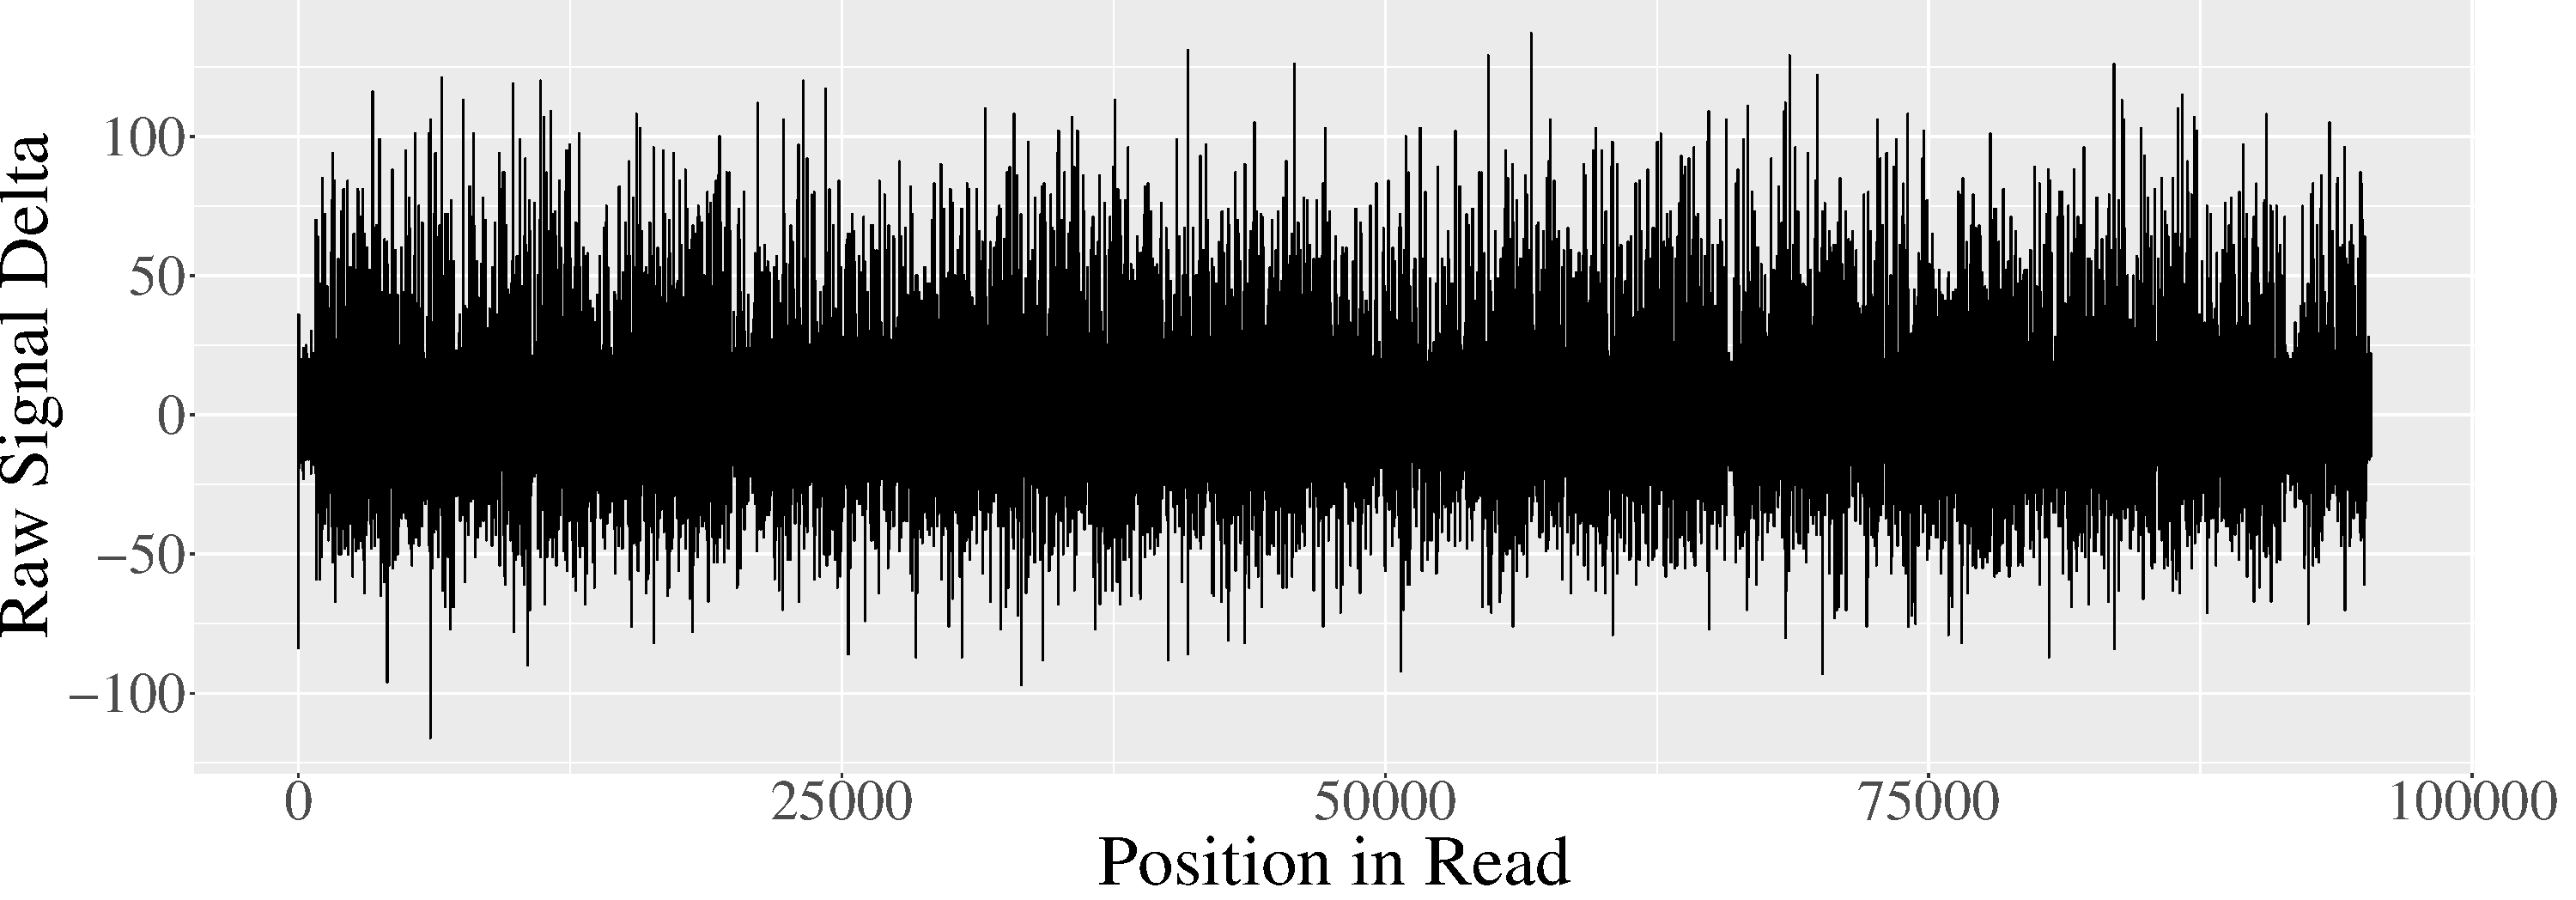
\includegraphics[scale=0.31]{plots/reads.e9f08690-171f-476f-9119-5330d0290126.raw.delta.pdf}
	\caption{\label{fig:read-e9f-delta}The deltas of the read with ID e9f08690-171f-476f-9119-5330d0290126. $-4, -2, -10, 16,\dots$ is the sequence starting from position 25000.}
\end{figure}


%in Section \ref{sec:}
As previously discussed, differential coding has been applied to the compression of nanopore signal data.
Let's now consider the deltas between each read data point. Figure \ref{fig:read-e9f-delta} plots the differential encoding of the read with ID e9f08690-171f-476f-9119-5330d0290126. In comparison to the standard representation, as shown in Figure \ref{fig:read-e9f-pa}, differential coding removes inconsistent shifts in the data such that it has fewer repeated outliers. For example, the upward shift around position 50000 in Figure \ref{fig:read-e9f-pa} is no longer clearly evident in the differential encoding.
% TODO plot of the shift before and after diff encoding
The deltas range from $-1159$ to 913 with a median, mean and mode of 0, and a standard deviation of $\sim$13. See Table \ref{tab:trans}.
The middle 99\% lies tightly in the range from $-46$ to 63 in a normal-like distribution. See Figure \ref{fig:delta-hist} for a histogram of the deltas.
Interestingly, $-2$ occurs $\sim23\times 10^6$ more times than $-1$ which is likely a result of the ADC.

Also, notice that there are more small negative than positive deltas in the histogram. This implies that there are more small decreases in the signal than increases.
\label{subsec:prob}
Next, notice that the right tail extends much further than the left tail in the histogram. This suggests that there are significantly more large positive than negative deltas. In other words, there are more large jumps in the signal than falls.
In fact, the probability that a delta is lesser than $-128$ and greater than 127 is $\sim6.0\times 10^{-6}$ and $\sim3.7\times 10^{-5}$ respectively. Combining both probabilities we find that the probability that a delta is outside of the signed 1 byte range is $\sim$0.004\%. This is very small and will be exploited in section \ref{sec:vbbe21}.

\begin{figure}
	\centering
% Created by tikzDevice version 0.12.3.1 on 2022-10-11 18:29:28
% !TEX encoding = UTF-8 Unicode
\begin{tikzpicture}[x=1pt,y=1pt]
\definecolor{fillColor}{RGB}{255,255,255}
\path[use as bounding box,fill=fillColor,fill opacity=0.00] (0,0) rectangle (361.35,361.35);
\begin{scope}
\path[clip] (  0.00,  0.00) rectangle (361.35,361.35);
\definecolor{drawColor}{RGB}{255,255,255}
\definecolor{fillColor}{RGB}{255,255,255}

\path[draw=drawColor,line width= 0.6pt,line join=round,line cap=round,fill=fillColor] (  0.00,  0.00) rectangle (361.35,361.35);
\end{scope}
\begin{scope}
\path[clip] ( 27.31, 30.69) rectangle (355.85,355.85);
\definecolor{fillColor}{gray}{0.92}

\path[fill=fillColor] ( 27.31, 30.69) rectangle (355.85,355.85);
\definecolor{drawColor}{RGB}{255,255,255}

\path[draw=drawColor,line width= 0.3pt,line join=round] ( 27.31, 87.91) --
	(355.85, 87.91);

\path[draw=drawColor,line width= 0.3pt,line join=round] ( 27.31,172.79) --
	(355.85,172.79);

\path[draw=drawColor,line width= 0.3pt,line join=round] ( 27.31,257.67) --
	(355.85,257.67);

\path[draw=drawColor,line width= 0.3pt,line join=round] ( 27.31,342.55) --
	(355.85,342.55);

\path[draw=drawColor,line width= 0.3pt,line join=round] ( 50.02, 30.69) --
	( 50.02,355.85);

\path[draw=drawColor,line width= 0.3pt,line join=round] (127.80, 30.69) --
	(127.80,355.85);

\path[draw=drawColor,line width= 0.3pt,line join=round] (205.58, 30.69) --
	(205.58,355.85);

\path[draw=drawColor,line width= 0.3pt,line join=round] (283.36, 30.69) --
	(283.36,355.85);

\path[draw=drawColor,line width= 0.6pt,line join=round] ( 27.31, 45.47) --
	(355.85, 45.47);

\path[draw=drawColor,line width= 0.6pt,line join=round] ( 27.31,130.35) --
	(355.85,130.35);

\path[draw=drawColor,line width= 0.6pt,line join=round] ( 27.31,215.23) --
	(355.85,215.23);

\path[draw=drawColor,line width= 0.6pt,line join=round] ( 27.31,300.11) --
	(355.85,300.11);

\path[draw=drawColor,line width= 0.6pt,line join=round] ( 88.91, 30.69) --
	( 88.91,355.85);

\path[draw=drawColor,line width= 0.6pt,line join=round] (166.69, 30.69) --
	(166.69,355.85);

\path[draw=drawColor,line width= 0.6pt,line join=round] (244.47, 30.69) --
	(244.47,355.85);

\path[draw=drawColor,line width= 0.6pt,line join=round] (322.25, 30.69) --
	(322.25,355.85);
\definecolor{fillColor}{gray}{0.35}

\path[fill=fillColor] ( 43.10, 45.47) rectangle ( 44.50, 45.56);

\path[fill=fillColor] ( 44.66, 45.47) rectangle ( 46.06, 45.57);

\path[fill=fillColor] ( 46.21, 45.47) rectangle ( 47.61, 45.58);

\path[fill=fillColor] ( 47.77, 45.47) rectangle ( 49.17, 45.60);

\path[fill=fillColor] ( 49.32, 45.47) rectangle ( 50.72, 45.61);

\path[fill=fillColor] ( 50.88, 45.47) rectangle ( 52.28, 45.63);

\path[fill=fillColor] ( 52.44, 45.47) rectangle ( 53.84, 45.64);

\path[fill=fillColor] ( 53.99, 45.47) rectangle ( 55.39, 45.68);

\path[fill=fillColor] ( 55.55, 45.47) rectangle ( 56.95, 45.68);

\path[fill=fillColor] ( 57.10, 45.47) rectangle ( 58.50, 45.71);

\path[fill=fillColor] ( 58.66, 45.47) rectangle ( 60.06, 45.73);

\path[fill=fillColor] ( 60.21, 45.47) rectangle ( 61.61, 45.78);

\path[fill=fillColor] ( 61.77, 45.47) rectangle ( 63.17, 45.79);

\path[fill=fillColor] ( 63.32, 45.47) rectangle ( 64.72, 45.83);

\path[fill=fillColor] ( 64.88, 45.47) rectangle ( 66.28, 45.85);

\path[fill=fillColor] ( 66.44, 45.47) rectangle ( 67.84, 45.96);

\path[fill=fillColor] ( 67.99, 45.47) rectangle ( 69.39, 45.93);

\path[fill=fillColor] ( 69.55, 45.47) rectangle ( 70.95, 46.00);

\path[fill=fillColor] ( 71.10, 45.47) rectangle ( 72.50, 46.04);

\path[fill=fillColor] ( 72.66, 45.47) rectangle ( 74.06, 46.15);

\path[fill=fillColor] ( 74.21, 45.47) rectangle ( 75.61, 46.15);

\path[fill=fillColor] ( 75.77, 45.47) rectangle ( 77.17, 46.23);

\path[fill=fillColor] ( 77.32, 45.47) rectangle ( 78.72, 46.30);

\path[fill=fillColor] ( 78.88, 45.47) rectangle ( 80.28, 46.43);

\path[fill=fillColor] ( 80.44, 45.47) rectangle ( 81.84, 46.46);

\path[fill=fillColor] ( 81.99, 45.47) rectangle ( 83.39, 46.55);

\path[fill=fillColor] ( 83.55, 45.47) rectangle ( 84.95, 46.62);

\path[fill=fillColor] ( 85.10, 45.47) rectangle ( 86.50, 46.83);

\path[fill=fillColor] ( 86.66, 45.47) rectangle ( 88.06, 46.83);

\path[fill=fillColor] ( 88.21, 45.47) rectangle ( 89.61, 46.98);

\path[fill=fillColor] ( 89.77, 45.47) rectangle ( 91.17, 47.04);

\path[fill=fillColor] ( 91.33, 45.47) rectangle ( 92.73, 47.44);

\path[fill=fillColor] ( 92.88, 45.47) rectangle ( 94.28, 47.32);

\path[fill=fillColor] ( 94.44, 45.47) rectangle ( 95.84, 47.53);

\path[fill=fillColor] ( 95.99, 45.47) rectangle ( 97.39, 47.64);

\path[fill=fillColor] ( 97.55, 45.47) rectangle ( 98.95, 48.02);

\path[fill=fillColor] ( 99.10, 45.47) rectangle (100.50, 47.99);

\path[fill=fillColor] (100.66, 45.47) rectangle (102.06, 48.22);

\path[fill=fillColor] (102.21, 45.47) rectangle (103.61, 48.41);

\path[fill=fillColor] (103.77, 45.47) rectangle (105.17, 48.84);

\path[fill=fillColor] (105.33, 45.47) rectangle (106.73, 48.85);

\path[fill=fillColor] (106.88, 45.47) rectangle (108.28, 49.09);

\path[fill=fillColor] (108.44, 45.47) rectangle (109.84, 49.29);

\path[fill=fillColor] (109.99, 45.47) rectangle (111.39, 49.91);

\path[fill=fillColor] (111.55, 45.47) rectangle (112.95, 49.82);

\path[fill=fillColor] (113.10, 45.47) rectangle (114.50, 50.23);

\path[fill=fillColor] (114.66, 45.47) rectangle (116.06, 50.35);

\path[fill=fillColor] (116.21, 45.47) rectangle (117.61, 51.57);

\path[fill=fillColor] (117.77, 45.47) rectangle (119.17, 51.09);

\path[fill=fillColor] (119.33, 45.47) rectangle (120.73, 51.69);

\path[fill=fillColor] (120.88, 45.47) rectangle (122.28, 51.98);

\path[fill=fillColor] (122.44, 45.47) rectangle (123.84, 53.10);

\path[fill=fillColor] (123.99, 45.47) rectangle (125.39, 53.04);

\path[fill=fillColor] (125.55, 45.47) rectangle (126.95, 53.79);

\path[fill=fillColor] (127.10, 45.47) rectangle (128.50, 54.48);

\path[fill=fillColor] (128.66, 45.47) rectangle (130.06, 56.04);

\path[fill=fillColor] (130.21, 45.47) rectangle (131.61, 56.39);

\path[fill=fillColor] (131.77, 45.47) rectangle (133.17, 57.64);

\path[fill=fillColor] (133.33, 45.47) rectangle (134.73, 58.91);

\path[fill=fillColor] (134.88, 45.47) rectangle (136.28, 62.09);

\path[fill=fillColor] (136.44, 45.47) rectangle (137.84, 62.94);

\path[fill=fillColor] (137.99, 45.47) rectangle (139.39, 66.20);

\path[fill=fillColor] (139.55, 45.47) rectangle (140.95, 68.66);

\path[fill=fillColor] (141.10, 45.47) rectangle (142.50, 77.56);

\path[fill=fillColor] (142.66, 45.47) rectangle (144.06, 78.83);

\path[fill=fillColor] (144.21, 45.47) rectangle (145.61, 86.74);

\path[fill=fillColor] (145.77, 45.47) rectangle (147.17, 93.85);

\path[fill=fillColor] (147.33, 45.47) rectangle (148.73,109.71);

\path[fill=fillColor] (148.88, 45.47) rectangle (150.28,117.21);

\path[fill=fillColor] (150.44, 45.47) rectangle (151.84,133.18);

\path[fill=fillColor] (151.99, 45.47) rectangle (153.39,150.23);

\path[fill=fillColor] (153.55, 45.47) rectangle (154.95,179.85);

\path[fill=fillColor] (155.10, 45.47) rectangle (156.50,193.42);

\path[fill=fillColor] (156.66, 45.47) rectangle (158.06,217.30);

\path[fill=fillColor] (158.21, 45.47) rectangle (159.61,237.62);

\path[fill=fillColor] (159.77, 45.47) rectangle (161.17,279.04);

\path[fill=fillColor] (161.33, 45.47) rectangle (162.73,278.42);

\path[fill=fillColor] (162.88, 45.47) rectangle (164.28,298.06);

\path[fill=fillColor] (164.44, 45.47) rectangle (165.84,295.99);

\path[fill=fillColor] (165.99, 45.47) rectangle (167.39,341.07);

\path[fill=fillColor] (167.55, 45.47) rectangle (168.95,290.06);

\path[fill=fillColor] (169.10, 45.47) rectangle (170.50,287.04);

\path[fill=fillColor] (170.66, 45.47) rectangle (172.06,263.87);

\path[fill=fillColor] (172.21, 45.47) rectangle (173.61,260.44);

\path[fill=fillColor] (173.77, 45.47) rectangle (175.17,219.45);

\path[fill=fillColor] (175.33, 45.47) rectangle (176.73,199.09);

\path[fill=fillColor] (176.88, 45.47) rectangle (178.28,176.41);

\path[fill=fillColor] (178.44, 45.47) rectangle (179.84,163.55);

\path[fill=fillColor] (179.99, 45.47) rectangle (181.39,137.05);

\path[fill=fillColor] (181.55, 45.47) rectangle (182.95,121.98);

\path[fill=fillColor] (183.10, 45.47) rectangle (184.50,108.01);

\path[fill=fillColor] (184.66, 45.47) rectangle (186.06,101.52);

\path[fill=fillColor] (186.21, 45.47) rectangle (187.61, 87.73);

\path[fill=fillColor] (187.77, 45.47) rectangle (189.17, 81.57);

\path[fill=fillColor] (189.33, 45.47) rectangle (190.73, 74.66);

\path[fill=fillColor] (190.88, 45.47) rectangle (192.28, 73.54);

\path[fill=fillColor] (192.44, 45.47) rectangle (193.84, 65.72);

\path[fill=fillColor] (193.99, 45.47) rectangle (195.39, 63.51);

\path[fill=fillColor] (195.55, 45.47) rectangle (196.95, 60.61);

\path[fill=fillColor] (197.10, 45.47) rectangle (198.50, 59.78);

\path[fill=fillColor] (198.66, 45.47) rectangle (200.06, 56.96);

\path[fill=fillColor] (200.22, 45.47) rectangle (201.62, 55.81);

\path[fill=fillColor] (201.77, 45.47) rectangle (203.17, 54.68);

\path[fill=fillColor] (203.33, 45.47) rectangle (204.73, 54.31);

\path[fill=fillColor] (204.88, 45.47) rectangle (206.28, 52.96);

\path[fill=fillColor] (206.44, 45.47) rectangle (207.84, 52.35);

\path[fill=fillColor] (207.99, 45.47) rectangle (209.39, 51.71);

\path[fill=fillColor] (209.55, 45.47) rectangle (210.95, 51.74);

\path[fill=fillColor] (211.10, 45.47) rectangle (212.50, 50.81);

\path[fill=fillColor] (212.66, 45.47) rectangle (214.06, 50.58);

\path[fill=fillColor] (214.22, 45.47) rectangle (215.62, 50.10);

\path[fill=fillColor] (215.77, 45.47) rectangle (217.17, 50.51);

\path[fill=fillColor] (217.33, 45.47) rectangle (218.73, 49.54);

\path[fill=fillColor] (218.88, 45.47) rectangle (220.28, 49.47);

\path[fill=fillColor] (220.44, 45.47) rectangle (221.84, 49.16);

\path[fill=fillColor] (221.99, 45.47) rectangle (223.39, 49.28);

\path[fill=fillColor] (223.55, 45.47) rectangle (224.95, 48.80);

\path[fill=fillColor] (225.10, 45.47) rectangle (226.50, 48.68);

\path[fill=fillColor] (226.66, 45.47) rectangle (228.06, 48.51);

\path[fill=fillColor] (228.22, 45.47) rectangle (229.62, 48.57);

\path[fill=fillColor] (229.77, 45.47) rectangle (231.17, 48.24);

\path[fill=fillColor] (231.33, 45.47) rectangle (232.73, 48.13);

\path[fill=fillColor] (232.88, 45.47) rectangle (234.28, 47.97);

\path[fill=fillColor] (234.44, 45.47) rectangle (235.84, 48.07);

\path[fill=fillColor] (235.99, 45.47) rectangle (237.39, 47.76);

\path[fill=fillColor] (237.55, 45.47) rectangle (238.95, 47.72);

\path[fill=fillColor] (239.10, 45.47) rectangle (240.50, 47.55);

\path[fill=fillColor] (240.66, 45.47) rectangle (242.06, 47.78);

\path[fill=fillColor] (242.22, 45.47) rectangle (243.62, 47.39);

\path[fill=fillColor] (243.77, 45.47) rectangle (245.17, 47.39);

\path[fill=fillColor] (245.33, 45.47) rectangle (246.73, 47.26);

\path[fill=fillColor] (246.88, 45.47) rectangle (248.28, 47.35);

\path[fill=fillColor] (248.44, 45.47) rectangle (249.84, 47.14);

\path[fill=fillColor] (249.99, 45.47) rectangle (251.39, 47.09);

\path[fill=fillColor] (251.55, 45.47) rectangle (252.95, 47.03);

\path[fill=fillColor] (253.10, 45.47) rectangle (254.50, 47.07);

\path[fill=fillColor] (254.66, 45.47) rectangle (256.06, 46.91);

\path[fill=fillColor] (256.22, 45.47) rectangle (257.62, 46.86);

\path[fill=fillColor] (257.77, 45.47) rectangle (259.17, 46.79);

\path[fill=fillColor] (259.33, 45.47) rectangle (260.73, 46.85);

\path[fill=fillColor] (260.88, 45.47) rectangle (262.28, 46.68);

\path[fill=fillColor] (262.44, 45.47) rectangle (263.84, 46.66);

\path[fill=fillColor] (263.99, 45.47) rectangle (265.39, 46.58);

\path[fill=fillColor] (265.55, 45.47) rectangle (266.95, 46.71);

\path[fill=fillColor] (267.10, 45.47) rectangle (268.50, 46.49);

\path[fill=fillColor] (268.66, 45.47) rectangle (270.06, 46.48);

\path[fill=fillColor] (270.22, 45.47) rectangle (271.62, 46.42);

\path[fill=fillColor] (271.77, 45.47) rectangle (273.17, 46.46);

\path[fill=fillColor] (273.33, 45.47) rectangle (274.73, 46.35);

\path[fill=fillColor] (274.88, 45.47) rectangle (276.28, 46.32);

\path[fill=fillColor] (276.44, 45.47) rectangle (277.84, 46.28);

\path[fill=fillColor] (277.99, 45.47) rectangle (279.39, 46.31);

\path[fill=fillColor] (279.55, 45.47) rectangle (280.95, 46.22);

\path[fill=fillColor] (281.10, 45.47) rectangle (282.50, 46.20);

\path[fill=fillColor] (282.66, 45.47) rectangle (284.06, 46.16);

\path[fill=fillColor] (284.22, 45.47) rectangle (285.62, 46.19);

\path[fill=fillColor] (285.77, 45.47) rectangle (287.17, 46.10);

\path[fill=fillColor] (287.33, 45.47) rectangle (288.73, 46.09);

\path[fill=fillColor] (288.88, 45.47) rectangle (290.28, 46.05);

\path[fill=fillColor] (290.44, 45.47) rectangle (291.84, 46.11);

\path[fill=fillColor] (291.99, 45.47) rectangle (293.39, 46.00);

\path[fill=fillColor] (293.55, 45.47) rectangle (294.95, 46.00);

\path[fill=fillColor] (295.10, 45.47) rectangle (296.50, 45.96);

\path[fill=fillColor] (296.66, 45.47) rectangle (298.06, 45.99);

\path[fill=fillColor] (298.22, 45.47) rectangle (299.62, 45.92);

\path[fill=fillColor] (299.77, 45.47) rectangle (301.17, 45.91);

\path[fill=fillColor] (301.33, 45.47) rectangle (302.73, 45.89);

\path[fill=fillColor] (302.88, 45.47) rectangle (304.28, 45.90);

\path[fill=fillColor] (304.44, 45.47) rectangle (305.84, 45.85);

\path[fill=fillColor] (305.99, 45.47) rectangle (307.39, 45.83);

\path[fill=fillColor] (307.55, 45.47) rectangle (308.95, 45.81);

\path[fill=fillColor] (309.11, 45.47) rectangle (310.51, 45.81);

\path[fill=fillColor] (310.66, 45.47) rectangle (312.06, 45.77);

\path[fill=fillColor] (312.22, 45.47) rectangle (313.62, 45.76);

\path[fill=fillColor] (313.77, 45.47) rectangle (315.17, 45.73);

\path[fill=fillColor] (315.33, 45.47) rectangle (316.73, 45.75);

\path[fill=fillColor] (316.88, 45.47) rectangle (318.28, 45.70);

\path[fill=fillColor] (318.44, 45.47) rectangle (319.84, 45.69);

\path[fill=fillColor] (319.99, 45.47) rectangle (321.39, 45.67);

\path[fill=fillColor] (321.55, 45.47) rectangle (322.95, 45.67);

\path[fill=fillColor] (323.11, 45.47) rectangle (324.51, 45.64);

\path[fill=fillColor] (324.66, 45.47) rectangle (326.06, 45.63);

\path[fill=fillColor] (326.22, 45.47) rectangle (327.62, 45.62);

\path[fill=fillColor] (327.77, 45.47) rectangle (329.17, 45.62);

\path[fill=fillColor] (329.33, 45.47) rectangle (330.73, 45.60);

\path[fill=fillColor] (330.88, 45.47) rectangle (332.28, 45.59);

\path[fill=fillColor] (332.44, 45.47) rectangle (333.84, 45.58);

\path[fill=fillColor] (333.99, 45.47) rectangle (335.39, 45.58);

\path[fill=fillColor] (335.55, 45.47) rectangle (336.95, 45.57);

\path[fill=fillColor] (337.11, 45.47) rectangle (338.51, 45.56);

\path[fill=fillColor] (338.66, 45.47) rectangle (340.06, 45.55);
\end{scope}
\begin{scope}
\path[clip] (  0.00,  0.00) rectangle (361.35,361.35);
\definecolor{drawColor}{gray}{0.30}

\node[text=drawColor,anchor=base east,inner sep=0pt, outer sep=0pt, scale=  0.88] at ( 22.36, 42.44) {0};

\node[text=drawColor,anchor=base east,inner sep=0pt, outer sep=0pt, scale=  0.88] at ( 22.36,127.32) {1};

\node[text=drawColor,anchor=base east,inner sep=0pt, outer sep=0pt, scale=  0.88] at ( 22.36,212.20) {2};

\node[text=drawColor,anchor=base east,inner sep=0pt, outer sep=0pt, scale=  0.88] at ( 22.36,297.08) {3};
\end{scope}
\begin{scope}
\path[clip] (  0.00,  0.00) rectangle (361.35,361.35);
\definecolor{drawColor}{gray}{0.20}

\path[draw=drawColor,line width= 0.6pt,line join=round] ( 24.56, 45.47) --
	( 27.31, 45.47);

\path[draw=drawColor,line width= 0.6pt,line join=round] ( 24.56,130.35) --
	( 27.31,130.35);

\path[draw=drawColor,line width= 0.6pt,line join=round] ( 24.56,215.23) --
	( 27.31,215.23);

\path[draw=drawColor,line width= 0.6pt,line join=round] ( 24.56,300.11) --
	( 27.31,300.11);
\end{scope}
\begin{scope}
\path[clip] (  0.00,  0.00) rectangle (361.35,361.35);
\definecolor{drawColor}{gray}{0.20}

\path[draw=drawColor,line width= 0.6pt,line join=round] ( 88.91, 27.94) --
	( 88.91, 30.69);

\path[draw=drawColor,line width= 0.6pt,line join=round] (166.69, 27.94) --
	(166.69, 30.69);

\path[draw=drawColor,line width= 0.6pt,line join=round] (244.47, 27.94) --
	(244.47, 30.69);

\path[draw=drawColor,line width= 0.6pt,line join=round] (322.25, 27.94) --
	(322.25, 30.69);
\end{scope}
\begin{scope}
\path[clip] (  0.00,  0.00) rectangle (361.35,361.35);
\definecolor{drawColor}{gray}{0.30}

\node[text=drawColor,anchor=base,inner sep=0pt, outer sep=0pt, scale=  0.88] at ( 88.91, 19.68) {-50};

\node[text=drawColor,anchor=base,inner sep=0pt, outer sep=0pt, scale=  0.88] at (166.69, 19.68) {0};

\node[text=drawColor,anchor=base,inner sep=0pt, outer sep=0pt, scale=  0.88] at (244.47, 19.68) {50};

\node[text=drawColor,anchor=base,inner sep=0pt, outer sep=0pt, scale=  0.88] at (322.25, 19.68) {100};
\end{scope}
\begin{scope}
\path[clip] (  0.00,  0.00) rectangle (361.35,361.35);
\definecolor{drawColor}{RGB}{0,0,0}

\node[text=drawColor,anchor=base,inner sep=0pt, outer sep=0pt, scale=  1.10] at (191.58,  7.64) {Raw Signal Delta};
\end{scope}
\begin{scope}
\path[clip] (  0.00,  0.00) rectangle (361.35,361.35);
\definecolor{drawColor}{RGB}{0,0,0}

\node[text=drawColor,rotate= 90.00,anchor=base,inner sep=0pt, outer sep=0pt, scale=  1.10] at ( 13.08,193.27) {Frequency ($\times 10^9$)};
\end{scope}
\end{tikzpicture}

	\caption{\label{fig:delta-hist}The frequency of raw signal deltas -80 to 112 in millions for the data set. The deltas outside this range occurred less than 1 million times.}
\end{figure}


\begin{figure}
\centering
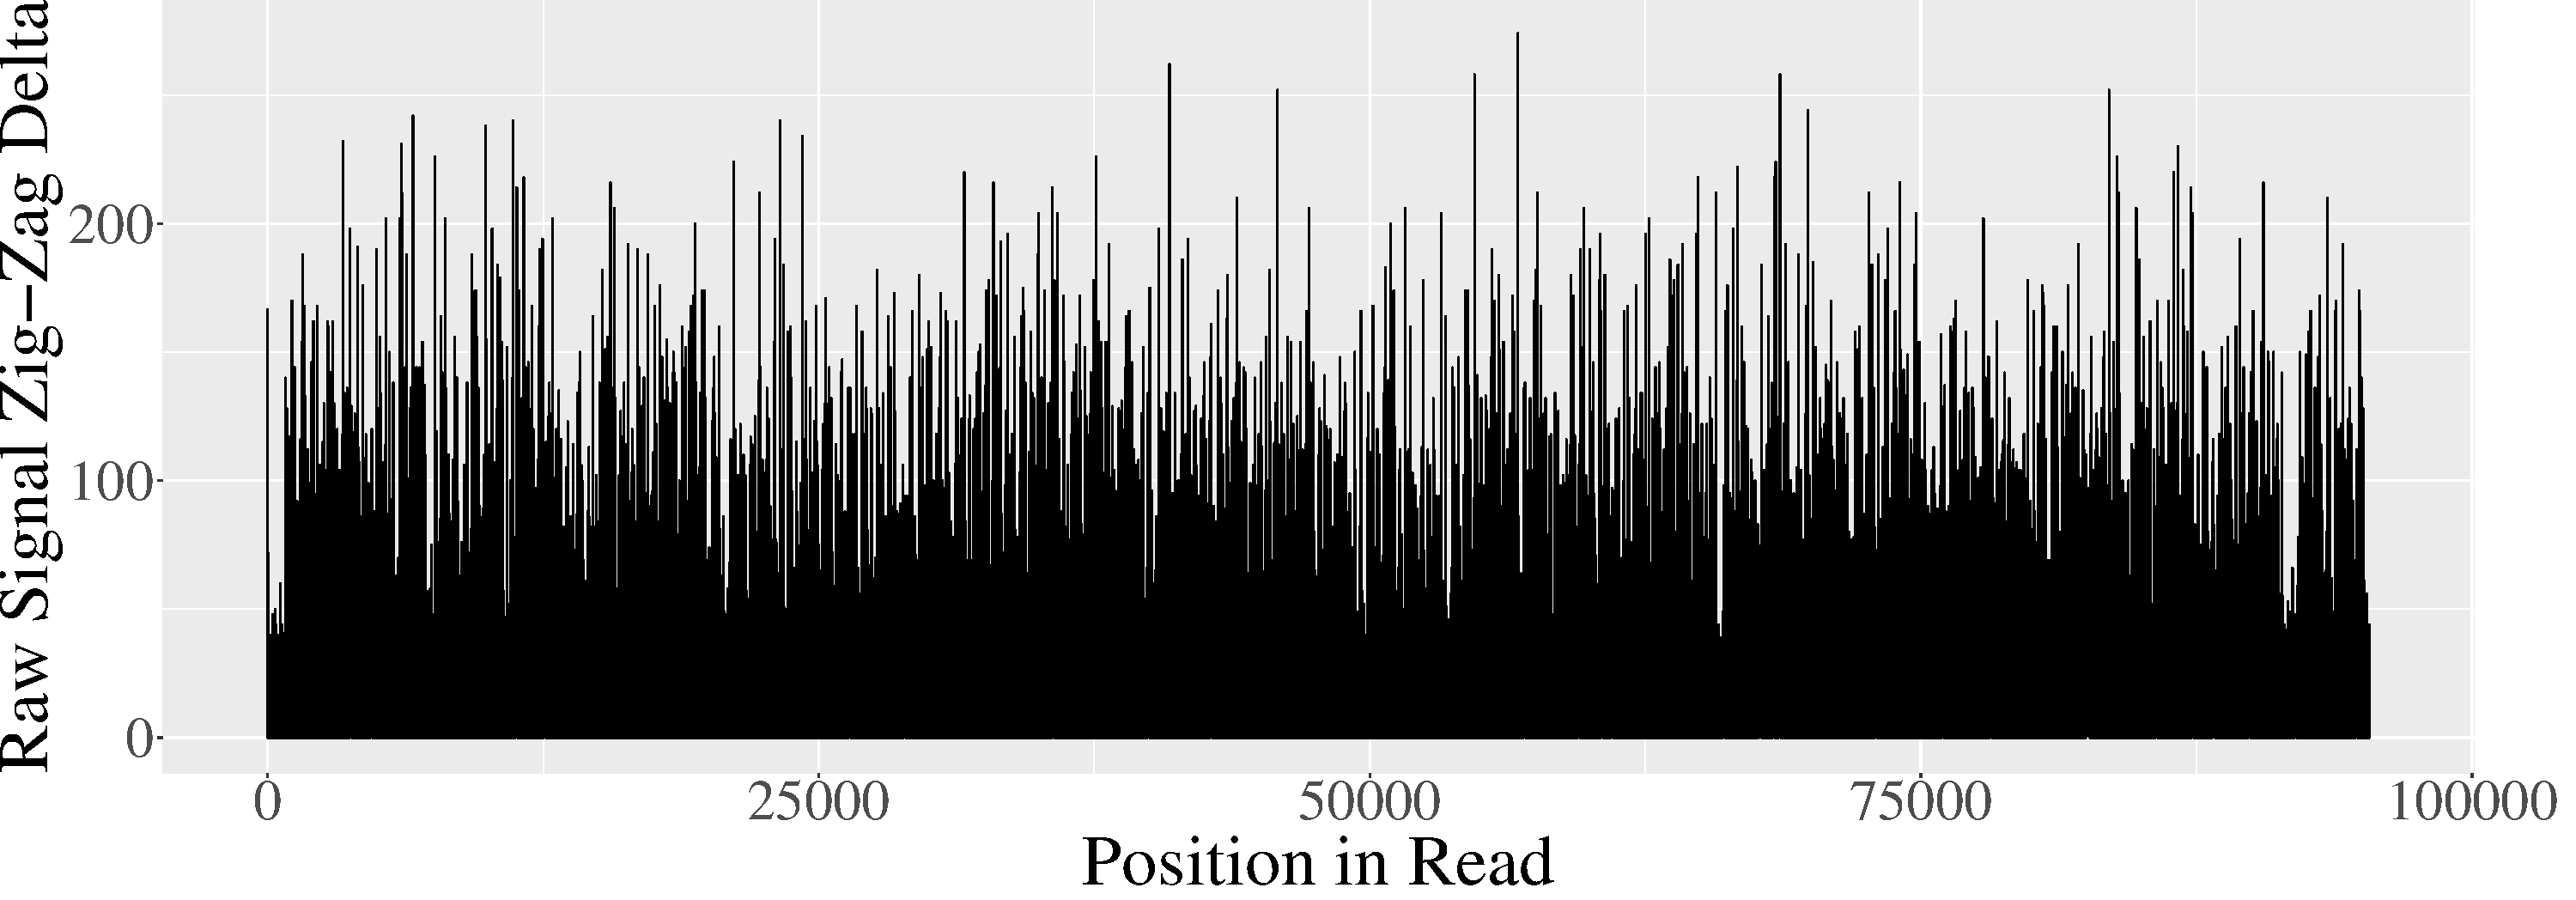
\includegraphics[scale=0.31]{plots/reads.e9f08690-171f-476f-9119-5330d0290126.raw.delta.zigzag.pdf}
	\caption[The zig-zag deltas of the read with ID e9f08690-171f-476f-9119-5330d0290126.]{\label{fig:read-e9f-zd}The zig-zag deltas of the read with ID e9f08690-171f-476f-9119-5330d0290126. $7, 3, 19, 32,\dots$ is the sequence starting from position 25000.}
\end{figure}


The zig-zag deltas (deltas then zig-zag encoding) range from 0 to 2317 with a median of 4, mean of $\sim15.5679$ and standard deviation of $\sim20.6060$. See Table \ref{tab:trans}. The zig-zag encoding interleaves the positive and negative deltas resulting in a geometric-like distribution which is not completely decreasing. See Figure \ref{fig:zd-hist}. Notice the `dotted' right tail; every box with an even offset from value 150 onwards is much larger than those with an odd offset. This is due to the higher frequency of large positive deltas in comparison to large negative deltas, as discussed above.
\label{subsec:stripe}

%\begin{figure}
%	\centering
% Created by tikzDevice version 0.12.3.1 on 2022-10-12 11:07:39
% !TEX encoding = UTF-8 Unicode
\begin{tikzpicture}[x=1pt,y=1pt]
\definecolor{fillColor}{RGB}{255,255,255}
\path[use as bounding box,fill=fillColor,fill opacity=0.00] (0,0) rectangle (361.35,361.35);
\begin{scope}
\path[clip] (  0.00,  0.00) rectangle (361.35,361.35);
\definecolor{drawColor}{RGB}{255,255,255}
\definecolor{fillColor}{RGB}{255,255,255}

\path[draw=drawColor,line width= 0.6pt,line join=round,line cap=round,fill=fillColor] (  0.00,  0.00) rectangle (361.35,361.35);
\end{scope}
\begin{scope}
\path[clip] ( 27.31, 30.69) rectangle (355.85,355.85);
\definecolor{fillColor}{gray}{0.92}

\path[fill=fillColor] ( 27.31, 30.69) rectangle (355.85,355.85);
\definecolor{drawColor}{RGB}{255,255,255}

\path[draw=drawColor,line width= 0.3pt,line join=round] ( 27.31, 87.91) --
	(355.85, 87.91);

\path[draw=drawColor,line width= 0.3pt,line join=round] ( 27.31,172.79) --
	(355.85,172.79);

\path[draw=drawColor,line width= 0.3pt,line join=round] ( 27.31,257.67) --
	(355.85,257.67);

\path[draw=drawColor,line width= 0.3pt,line join=round] ( 27.31,342.55) --
	(355.85,342.55);

\path[draw=drawColor,line width= 0.3pt,line join=round] ( 76.76, 30.69) --
	( 76.76,355.85);

\path[draw=drawColor,line width= 0.3pt,line join=round] (143.13, 30.69) --
	(143.13,355.85);

\path[draw=drawColor,line width= 0.3pt,line join=round] (209.50, 30.69) --
	(209.50,355.85);

\path[draw=drawColor,line width= 0.3pt,line join=round] (275.87, 30.69) --
	(275.87,355.85);

\path[draw=drawColor,line width= 0.3pt,line join=round] (342.24, 30.69) --
	(342.24,355.85);

\path[draw=drawColor,line width= 0.6pt,line join=round] ( 27.31, 45.47) --
	(355.85, 45.47);

\path[draw=drawColor,line width= 0.6pt,line join=round] ( 27.31,130.35) --
	(355.85,130.35);

\path[draw=drawColor,line width= 0.6pt,line join=round] ( 27.31,215.23) --
	(355.85,215.23);

\path[draw=drawColor,line width= 0.6pt,line join=round] ( 27.31,300.11) --
	(355.85,300.11);

\path[draw=drawColor,line width= 0.6pt,line join=round] ( 43.57, 30.69) --
	( 43.57,355.85);

\path[draw=drawColor,line width= 0.6pt,line join=round] (109.95, 30.69) --
	(109.95,355.85);

\path[draw=drawColor,line width= 0.6pt,line join=round] (176.32, 30.69) --
	(176.32,355.85);

\path[draw=drawColor,line width= 0.6pt,line join=round] (242.69, 30.69) --
	(242.69,355.85);

\path[draw=drawColor,line width= 0.6pt,line join=round] (309.06, 30.69) --
	(309.06,355.85);
\definecolor{fillColor}{gray}{0.35}

\path[fill=fillColor] ( 42.98, 45.47) rectangle ( 44.17,341.07);

\path[fill=fillColor] ( 44.30, 45.47) rectangle ( 45.50,295.99);

\path[fill=fillColor] ( 45.63, 45.47) rectangle ( 46.83,290.06);

\path[fill=fillColor] ( 46.96, 45.47) rectangle ( 48.15,298.06);

\path[fill=fillColor] ( 48.29, 45.47) rectangle ( 49.48,287.04);

\path[fill=fillColor] ( 49.61, 45.47) rectangle ( 50.81,278.42);

\path[fill=fillColor] ( 50.94, 45.47) rectangle ( 52.14,263.87);

\path[fill=fillColor] ( 52.27, 45.47) rectangle ( 53.46,279.04);

\path[fill=fillColor] ( 53.60, 45.47) rectangle ( 54.79,260.44);

\path[fill=fillColor] ( 54.92, 45.47) rectangle ( 56.12,237.62);

\path[fill=fillColor] ( 56.25, 45.47) rectangle ( 57.45,219.45);

\path[fill=fillColor] ( 57.58, 45.47) rectangle ( 58.77,217.30);

\path[fill=fillColor] ( 58.91, 45.47) rectangle ( 60.10,199.09);

\path[fill=fillColor] ( 60.23, 45.47) rectangle ( 61.43,193.42);

\path[fill=fillColor] ( 61.56, 45.47) rectangle ( 62.76,176.41);

\path[fill=fillColor] ( 62.89, 45.47) rectangle ( 64.08,179.85);

\path[fill=fillColor] ( 64.22, 45.47) rectangle ( 65.41,163.55);

\path[fill=fillColor] ( 65.54, 45.47) rectangle ( 66.74,150.23);

\path[fill=fillColor] ( 66.87, 45.47) rectangle ( 68.07,137.05);

\path[fill=fillColor] ( 68.20, 45.47) rectangle ( 69.39,133.18);

\path[fill=fillColor] ( 69.53, 45.47) rectangle ( 70.72,121.98);

\path[fill=fillColor] ( 70.85, 45.47) rectangle ( 72.05,117.21);

\path[fill=fillColor] ( 72.18, 45.47) rectangle ( 73.37,108.01);

\path[fill=fillColor] ( 73.51, 45.47) rectangle ( 74.70,109.71);

\path[fill=fillColor] ( 74.83, 45.47) rectangle ( 76.03,101.52);

\path[fill=fillColor] ( 76.16, 45.47) rectangle ( 77.36, 93.85);

\path[fill=fillColor] ( 77.49, 45.47) rectangle ( 78.68, 87.73);

\path[fill=fillColor] ( 78.82, 45.47) rectangle ( 80.01, 86.74);

\path[fill=fillColor] ( 80.14, 45.47) rectangle ( 81.34, 81.57);

\path[fill=fillColor] ( 81.47, 45.47) rectangle ( 82.67, 78.83);

\path[fill=fillColor] ( 82.80, 45.47) rectangle ( 83.99, 74.66);

\path[fill=fillColor] ( 84.13, 45.47) rectangle ( 85.32, 77.56);

\path[fill=fillColor] ( 85.45, 45.47) rectangle ( 86.65, 73.54);

\path[fill=fillColor] ( 86.78, 45.47) rectangle ( 87.98, 68.66);

\path[fill=fillColor] ( 88.11, 45.47) rectangle ( 89.30, 65.72);

\path[fill=fillColor] ( 89.44, 45.47) rectangle ( 90.63, 66.20);

\path[fill=fillColor] ( 90.76, 45.47) rectangle ( 91.96, 63.51);

\path[fill=fillColor] ( 92.09, 45.47) rectangle ( 93.29, 62.94);

\path[fill=fillColor] ( 93.42, 45.47) rectangle ( 94.61, 60.61);

\path[fill=fillColor] ( 94.75, 45.47) rectangle ( 95.94, 62.09);

\path[fill=fillColor] ( 96.07, 45.47) rectangle ( 97.27, 59.78);

\path[fill=fillColor] ( 97.40, 45.47) rectangle ( 98.60, 58.91);

\path[fill=fillColor] ( 98.73, 45.47) rectangle ( 99.92, 56.96);

\path[fill=fillColor] (100.06, 45.47) rectangle (101.25, 57.64);

\path[fill=fillColor] (101.38, 45.47) rectangle (102.58, 55.81);

\path[fill=fillColor] (102.71, 45.47) rectangle (103.91, 56.39);

\path[fill=fillColor] (104.04, 45.47) rectangle (105.23, 54.68);

\path[fill=fillColor] (105.37, 45.47) rectangle (106.56, 56.04);

\path[fill=fillColor] (106.69, 45.47) rectangle (107.89, 54.31);

\path[fill=fillColor] (108.02, 45.47) rectangle (109.22, 54.48);

\path[fill=fillColor] (109.35, 45.47) rectangle (110.54, 52.96);

\path[fill=fillColor] (110.68, 45.47) rectangle (111.87, 53.79);

\path[fill=fillColor] (112.00, 45.47) rectangle (113.20, 52.35);

\path[fill=fillColor] (113.33, 45.47) rectangle (114.52, 53.04);

\path[fill=fillColor] (114.66, 45.47) rectangle (115.85, 51.71);

\path[fill=fillColor] (115.99, 45.47) rectangle (117.18, 53.10);

\path[fill=fillColor] (117.31, 45.47) rectangle (118.51, 51.74);

\path[fill=fillColor] (118.64, 45.47) rectangle (119.83, 51.98);

\path[fill=fillColor] (119.97, 45.47) rectangle (121.16, 50.81);

\path[fill=fillColor] (121.29, 45.47) rectangle (122.49, 51.69);

\path[fill=fillColor] (122.62, 45.47) rectangle (123.82, 50.58);

\path[fill=fillColor] (123.95, 45.47) rectangle (125.14, 51.09);

\path[fill=fillColor] (125.28, 45.47) rectangle (126.47, 50.10);

\path[fill=fillColor] (126.60, 45.47) rectangle (127.80, 51.57);

\path[fill=fillColor] (127.93, 45.47) rectangle (129.13, 50.51);

\path[fill=fillColor] (129.26, 45.47) rectangle (130.45, 50.35);

\path[fill=fillColor] (130.59, 45.47) rectangle (131.78, 49.54);

\path[fill=fillColor] (131.91, 45.47) rectangle (133.11, 50.23);

\path[fill=fillColor] (133.24, 45.47) rectangle (134.44, 49.47);

\path[fill=fillColor] (134.57, 45.47) rectangle (135.76, 49.82);

\path[fill=fillColor] (135.90, 45.47) rectangle (137.09, 49.16);

\path[fill=fillColor] (137.22, 45.47) rectangle (138.42, 49.91);

\path[fill=fillColor] (138.55, 45.47) rectangle (139.75, 49.28);

\path[fill=fillColor] (139.88, 45.47) rectangle (141.07, 49.29);

\path[fill=fillColor] (141.21, 45.47) rectangle (142.40, 48.80);

\path[fill=fillColor] (142.53, 45.47) rectangle (143.73, 49.09);

\path[fill=fillColor] (143.86, 45.47) rectangle (145.06, 48.68);

\path[fill=fillColor] (145.19, 45.47) rectangle (146.38, 48.85);

\path[fill=fillColor] (146.52, 45.47) rectangle (147.71, 48.51);

\path[fill=fillColor] (147.84, 45.47) rectangle (149.04, 48.84);

\path[fill=fillColor] (149.17, 45.47) rectangle (150.37, 48.57);

\path[fill=fillColor] (150.50, 45.47) rectangle (151.69, 48.41);

\path[fill=fillColor] (151.83, 45.47) rectangle (153.02, 48.24);

\path[fill=fillColor] (153.15, 45.47) rectangle (154.35, 48.22);

\path[fill=fillColor] (154.48, 45.47) rectangle (155.67, 48.13);

\path[fill=fillColor] (155.81, 45.47) rectangle (157.00, 47.99);

\path[fill=fillColor] (157.14, 45.47) rectangle (158.33, 47.97);

\path[fill=fillColor] (158.46, 45.47) rectangle (159.66, 48.02);

\path[fill=fillColor] (159.79, 45.47) rectangle (160.98, 48.07);

\path[fill=fillColor] (161.12, 45.47) rectangle (162.31, 47.64);

\path[fill=fillColor] (162.44, 45.47) rectangle (163.64, 47.76);

\path[fill=fillColor] (163.77, 45.47) rectangle (164.97, 47.53);

\path[fill=fillColor] (165.10, 45.47) rectangle (166.29, 47.72);

\path[fill=fillColor] (166.43, 45.47) rectangle (167.62, 47.32);

\path[fill=fillColor] (167.75, 45.47) rectangle (168.95, 47.55);

\path[fill=fillColor] (169.08, 45.47) rectangle (170.28, 47.44);

\path[fill=fillColor] (170.41, 45.47) rectangle (171.60, 47.78);

\path[fill=fillColor] (171.74, 45.47) rectangle (172.93, 47.04);

\path[fill=fillColor] (173.06, 45.47) rectangle (174.26, 47.39);

\path[fill=fillColor] (174.39, 45.47) rectangle (175.59, 46.98);

\path[fill=fillColor] (175.72, 45.47) rectangle (176.91, 47.39);

\path[fill=fillColor] (177.05, 45.47) rectangle (178.24, 46.83);

\path[fill=fillColor] (178.37, 45.47) rectangle (179.57, 47.26);

\path[fill=fillColor] (179.70, 45.47) rectangle (180.90, 46.83);

\path[fill=fillColor] (181.03, 45.47) rectangle (182.22, 47.35);

\path[fill=fillColor] (182.36, 45.47) rectangle (183.55, 46.62);

\path[fill=fillColor] (183.68, 45.47) rectangle (184.88, 47.14);

\path[fill=fillColor] (185.01, 45.47) rectangle (186.21, 46.55);

\path[fill=fillColor] (186.34, 45.47) rectangle (187.53, 47.09);

\path[fill=fillColor] (187.67, 45.47) rectangle (188.86, 46.46);

\path[fill=fillColor] (188.99, 45.47) rectangle (190.19, 47.03);

\path[fill=fillColor] (190.32, 45.47) rectangle (191.52, 46.43);

\path[fill=fillColor] (191.65, 45.47) rectangle (192.84, 47.07);

\path[fill=fillColor] (192.98, 45.47) rectangle (194.17, 46.30);

\path[fill=fillColor] (194.30, 45.47) rectangle (195.50, 46.91);

\path[fill=fillColor] (195.63, 45.47) rectangle (196.82, 46.23);

\path[fill=fillColor] (196.96, 45.47) rectangle (198.15, 46.86);

\path[fill=fillColor] (198.29, 45.47) rectangle (199.48, 46.15);

\path[fill=fillColor] (199.61, 45.47) rectangle (200.81, 46.79);

\path[fill=fillColor] (200.94, 45.47) rectangle (202.13, 46.15);

\path[fill=fillColor] (202.27, 45.47) rectangle (203.46, 46.85);

\path[fill=fillColor] (203.59, 45.47) rectangle (204.79, 46.04);

\path[fill=fillColor] (204.92, 45.47) rectangle (206.12, 46.68);

\path[fill=fillColor] (206.25, 45.47) rectangle (207.44, 46.00);

\path[fill=fillColor] (207.58, 45.47) rectangle (208.77, 46.66);

\path[fill=fillColor] (208.90, 45.47) rectangle (210.10, 45.93);

\path[fill=fillColor] (210.23, 45.47) rectangle (211.43, 46.58);

\path[fill=fillColor] (211.56, 45.47) rectangle (212.75, 45.96);

\path[fill=fillColor] (212.89, 45.47) rectangle (214.08, 46.71);

\path[fill=fillColor] (214.21, 45.47) rectangle (215.41, 45.85);

\path[fill=fillColor] (215.54, 45.47) rectangle (216.74, 46.49);

\path[fill=fillColor] (216.87, 45.47) rectangle (218.06, 45.83);

\path[fill=fillColor] (218.20, 45.47) rectangle (219.39, 46.48);

\path[fill=fillColor] (219.52, 45.47) rectangle (220.72, 45.79);

\path[fill=fillColor] (220.85, 45.47) rectangle (222.05, 46.42);

\path[fill=fillColor] (222.18, 45.47) rectangle (223.37, 45.78);

\path[fill=fillColor] (223.51, 45.47) rectangle (224.70, 46.46);

\path[fill=fillColor] (224.83, 45.47) rectangle (226.03, 45.73);

\path[fill=fillColor] (226.16, 45.47) rectangle (227.36, 46.35);

\path[fill=fillColor] (227.49, 45.47) rectangle (228.68, 45.71);

\path[fill=fillColor] (228.82, 45.47) rectangle (230.01, 46.32);

\path[fill=fillColor] (230.14, 45.47) rectangle (231.34, 45.68);

\path[fill=fillColor] (231.47, 45.47) rectangle (232.67, 46.28);

\path[fill=fillColor] (232.80, 45.47) rectangle (233.99, 45.68);

\path[fill=fillColor] (234.13, 45.47) rectangle (235.32, 46.31);

\path[fill=fillColor] (235.45, 45.47) rectangle (236.65, 45.64);

\path[fill=fillColor] (236.78, 45.47) rectangle (237.98, 46.22);

\path[fill=fillColor] (238.11, 45.47) rectangle (239.30, 45.63);

\path[fill=fillColor] (239.44, 45.47) rectangle (240.63, 46.20);

\path[fill=fillColor] (240.76, 45.47) rectangle (241.96, 45.61);

\path[fill=fillColor] (242.09, 45.47) rectangle (243.28, 46.16);

\path[fill=fillColor] (243.42, 45.47) rectangle (244.61, 45.60);

\path[fill=fillColor] (244.74, 45.47) rectangle (245.94, 46.19);

\path[fill=fillColor] (246.07, 45.47) rectangle (247.27, 45.58);

\path[fill=fillColor] (247.40, 45.47) rectangle (248.59, 46.10);

\path[fill=fillColor] (248.73, 45.47) rectangle (249.92, 45.57);

\path[fill=fillColor] (250.05, 45.47) rectangle (251.25, 46.09);

\path[fill=fillColor] (251.38, 45.47) rectangle (252.58, 45.56);

\path[fill=fillColor] (252.71, 45.47) rectangle (253.90, 46.05);

\path[fill=fillColor] (254.04, 45.47) rectangle (255.23, 45.56);

\path[fill=fillColor] (255.36, 45.47) rectangle (256.56, 46.11);

\path[fill=fillColor] (256.69, 45.47) rectangle (257.89, 45.54);

\path[fill=fillColor] (258.02, 45.47) rectangle (259.21, 46.00);

\path[fill=fillColor] (259.35, 45.47) rectangle (260.54, 45.53);

\path[fill=fillColor] (260.67, 45.47) rectangle (261.87, 46.00);

\path[fill=fillColor] (262.00, 45.47) rectangle (263.20, 45.53);

\path[fill=fillColor] (263.33, 45.47) rectangle (264.52, 45.96);

\path[fill=fillColor] (264.66, 45.47) rectangle (265.85, 45.52);

\path[fill=fillColor] (265.98, 45.47) rectangle (267.18, 45.99);

\path[fill=fillColor] (267.31, 45.47) rectangle (268.51, 45.51);

\path[fill=fillColor] (268.64, 45.47) rectangle (269.83, 45.92);

\path[fill=fillColor] (269.97, 45.47) rectangle (271.16, 45.51);

\path[fill=fillColor] (271.29, 45.47) rectangle (272.49, 45.91);

\path[fill=fillColor] (272.62, 45.47) rectangle (273.82, 45.51);

\path[fill=fillColor] (273.95, 45.47) rectangle (275.14, 45.89);

\path[fill=fillColor] (275.28, 45.47) rectangle (276.47, 45.50);

\path[fill=fillColor] (276.60, 45.47) rectangle (277.80, 45.90);

\path[fill=fillColor] (277.93, 45.47) rectangle (279.13, 45.50);

\path[fill=fillColor] (279.26, 45.47) rectangle (280.45, 45.85);

\path[fill=fillColor] (280.59, 45.47) rectangle (281.78, 45.49);

\path[fill=fillColor] (281.91, 45.47) rectangle (283.11, 45.83);

\path[fill=fillColor] (283.24, 45.47) rectangle (284.43, 45.49);

\path[fill=fillColor] (284.57, 45.47) rectangle (285.76, 45.81);

\path[fill=fillColor] (285.89, 45.47) rectangle (287.09, 45.49);

\path[fill=fillColor] (287.22, 45.47) rectangle (288.42, 45.81);

\path[fill=fillColor] (288.55, 45.47) rectangle (289.74, 45.49);

\path[fill=fillColor] (289.88, 45.47) rectangle (291.07, 45.77);

\path[fill=fillColor] (291.20, 45.47) rectangle (292.40, 45.48);

\path[fill=fillColor] (292.53, 45.47) rectangle (293.73, 45.76);

\path[fill=fillColor] (293.86, 45.47) rectangle (295.05, 45.48);

\path[fill=fillColor] (295.19, 45.47) rectangle (296.38, 45.73);

\path[fill=fillColor] (296.51, 45.47) rectangle (297.71, 45.48);

\path[fill=fillColor] (297.84, 45.47) rectangle (299.04, 45.75);

\path[fill=fillColor] (299.17, 45.47) rectangle (300.36, 45.48);

\path[fill=fillColor] (300.50, 45.47) rectangle (301.69, 45.70);

\path[fill=fillColor] (301.82, 45.47) rectangle (303.02, 45.48);

\path[fill=fillColor] (303.15, 45.47) rectangle (304.35, 45.69);

\path[fill=fillColor] (304.48, 45.47) rectangle (305.67, 45.48);

\path[fill=fillColor] (305.81, 45.47) rectangle (307.00, 45.67);

\path[fill=fillColor] (307.13, 45.47) rectangle (308.33, 45.48);

\path[fill=fillColor] (308.46, 45.47) rectangle (309.66, 45.67);

\path[fill=fillColor] (309.79, 45.47) rectangle (310.98, 45.47);

\path[fill=fillColor] (311.12, 45.47) rectangle (312.31, 45.64);

\path[fill=fillColor] (312.44, 45.47) rectangle (313.64, 45.47);

\path[fill=fillColor] (313.77, 45.47) rectangle (314.97, 45.63);

\path[fill=fillColor] (315.10, 45.47) rectangle (316.29, 45.47);

\path[fill=fillColor] (316.43, 45.47) rectangle (317.62, 45.62);

\path[fill=fillColor] (317.75, 45.47) rectangle (318.95, 45.47);

\path[fill=fillColor] (319.08, 45.47) rectangle (320.28, 45.62);

\path[fill=fillColor] (320.41, 45.47) rectangle (321.60, 45.47);

\path[fill=fillColor] (321.74, 45.47) rectangle (322.93, 45.60);

\path[fill=fillColor] (323.06, 45.47) rectangle (324.26, 45.47);

\path[fill=fillColor] (324.39, 45.47) rectangle (325.58, 45.59);

\path[fill=fillColor] (325.72, 45.47) rectangle (326.91, 45.47);

\path[fill=fillColor] (327.04, 45.47) rectangle (328.24, 45.58);

\path[fill=fillColor] (328.37, 45.47) rectangle (329.57, 45.47);

\path[fill=fillColor] (329.70, 45.47) rectangle (330.89, 45.58);

\path[fill=fillColor] (331.03, 45.47) rectangle (332.22, 45.47);

\path[fill=fillColor] (332.35, 45.47) rectangle (333.55, 45.57);

\path[fill=fillColor] (333.68, 45.47) rectangle (334.88, 45.47);

\path[fill=fillColor] (335.01, 45.47) rectangle (336.20, 45.56);

\path[fill=fillColor] (336.34, 45.47) rectangle (337.53, 45.47);

\path[fill=fillColor] (337.66, 45.47) rectangle (338.86, 45.55);

\path[fill=fillColor] (338.99, 45.47) rectangle (340.19, 45.47);
\end{scope}
\begin{scope}
\path[clip] (  0.00,  0.00) rectangle (361.35,361.35);
\definecolor{drawColor}{gray}{0.30}

\node[text=drawColor,anchor=base east,inner sep=0pt, outer sep=0pt, scale=  0.88] at ( 22.36, 42.44) {0};

\node[text=drawColor,anchor=base east,inner sep=0pt, outer sep=0pt, scale=  0.88] at ( 22.36,127.32) {1};

\node[text=drawColor,anchor=base east,inner sep=0pt, outer sep=0pt, scale=  0.88] at ( 22.36,212.20) {2};

\node[text=drawColor,anchor=base east,inner sep=0pt, outer sep=0pt, scale=  0.88] at ( 22.36,297.08) {3};
\end{scope}
\begin{scope}
\path[clip] (  0.00,  0.00) rectangle (361.35,361.35);
\definecolor{drawColor}{gray}{0.20}

\path[draw=drawColor,line width= 0.6pt,line join=round] ( 24.56, 45.47) --
	( 27.31, 45.47);

\path[draw=drawColor,line width= 0.6pt,line join=round] ( 24.56,130.35) --
	( 27.31,130.35);

\path[draw=drawColor,line width= 0.6pt,line join=round] ( 24.56,215.23) --
	( 27.31,215.23);

\path[draw=drawColor,line width= 0.6pt,line join=round] ( 24.56,300.11) --
	( 27.31,300.11);
\end{scope}
\begin{scope}
\path[clip] (  0.00,  0.00) rectangle (361.35,361.35);
\definecolor{drawColor}{gray}{0.20}

\path[draw=drawColor,line width= 0.6pt,line join=round] ( 43.57, 27.94) --
	( 43.57, 30.69);

\path[draw=drawColor,line width= 0.6pt,line join=round] (109.95, 27.94) --
	(109.95, 30.69);

\path[draw=drawColor,line width= 0.6pt,line join=round] (176.32, 27.94) --
	(176.32, 30.69);

\path[draw=drawColor,line width= 0.6pt,line join=round] (242.69, 27.94) --
	(242.69, 30.69);

\path[draw=drawColor,line width= 0.6pt,line join=round] (309.06, 27.94) --
	(309.06, 30.69);
\end{scope}
\begin{scope}
\path[clip] (  0.00,  0.00) rectangle (361.35,361.35);
\definecolor{drawColor}{gray}{0.30}

\node[text=drawColor,anchor=base,inner sep=0pt, outer sep=0pt, scale=  0.88] at ( 43.57, 19.68) {0};

\node[text=drawColor,anchor=base,inner sep=0pt, outer sep=0pt, scale=  0.88] at (109.95, 19.68) {50};

\node[text=drawColor,anchor=base,inner sep=0pt, outer sep=0pt, scale=  0.88] at (176.32, 19.68) {100};

\node[text=drawColor,anchor=base,inner sep=0pt, outer sep=0pt, scale=  0.88] at (242.69, 19.68) {150};

\node[text=drawColor,anchor=base,inner sep=0pt, outer sep=0pt, scale=  0.88] at (309.06, 19.68) {200};
\end{scope}
\begin{scope}
\path[clip] (  0.00,  0.00) rectangle (361.35,361.35);
\definecolor{drawColor}{RGB}{0,0,0}

\node[text=drawColor,anchor=base,inner sep=0pt, outer sep=0pt, scale=  1.10] at (191.58,  7.64) {Raw Signal Zig-Zag Delta};
\end{scope}
\begin{scope}
\path[clip] (  0.00,  0.00) rectangle (361.35,361.35);
\definecolor{drawColor}{RGB}{0,0,0}

\node[text=drawColor,rotate= 90.00,anchor=base,inner sep=0pt, outer sep=0pt, scale=  1.10] at ( 13.08,193.27) {Frequency ($\times 10^9$)};
\end{scope}
\end{tikzpicture}

%	\caption[The frequency of raw signal zig-zag deltas.]{\label{fig:zd-hist}The frequency of raw signal zig-zag deltas 0 to 224 in millions for the data set. The zig-zag deltas outside this range occurred less than 1 million times.}
%\end{figure}


To observe the positive effect that differential coding has on the compression
of nanopore signal data, let's calculate the entropy of the data before and
after the delta transformations. This assumes the data is generated by an
independent and identically distributed random variable which follows the data's
distribution. Table \ref{tab:entropy} shows the resulting calculations. On
average for the whole data set, the entropy is 7.70 bits per data point compared
to 5.39 for the delta and zig-zag delta transformations. This is a difference of
2.31 bits per point which is quite large and clearly demonstrates how
differential coding helps take the distribution closer to its true entropy which
is unknown. From this it is clear that downstream entropy coding methods would
benefit from operating on the deltas rather than the original raw signal data.

\begin{table}
    \caption{\label{tab:entropy} The entropy of the data and its transformations.}
    \begin{tabular}{|l|l|}
        \hline
	    Transformation & Entropy (bits per point)\\
        \hline
None & 7.699965\\
Delta & 5.391453\\
Zig-Zag Delta & 5.391453\\
	\hline
    \end{tabular}
\end{table}


% submin
% zsubmean
% zsubmedian

%\chapter{Experiments} \label{chap:experiments}

The experiments go here.


\chapter{Problem Space} \label{chap:probspace}

\section{The Focus}

%TODO why lossless important
%TODO why not lossy
%TODO why per read

It is important for fast parallel querying that the reads are compressed separately. That's not to say that each read is independent. Reads originating from the same channel and well/pore will have been recorded by the same sensor and so will likely have similar properties. This is especially true for reads recorded at a similar timestamp as each channel deteriorates over the course of a sequencing run. A compression method may take advantage of these available patterns but it is important for querying that each read can be decompressed independently. Perhaps there exists a multi-read compression strategy which is great for space reduction and hence archival purposes. However, such a strategy is not obvious and the primary desire of bioinformaticians is a better compression algorithm that does not sacrifice parallel querying. Hence, multi-read compression is outside the scope of this thesis.

Lossy compression, although an interesting avenue, is not desirable for most research applications where accuracy is more valued than storage space. For example, long-term archival of scholarly research data must be lossless to allow for public replication of any results. For this reason, lossless compression is the focus of this thesis.


% Explore integer methods without generic

Instead, each integer can be represented more space-efficiently by using $b<16$ bits where \[b(x)=\lceil\log_2(\max(x))\rceil.\] In this case, the compression ratio would be approximately $16/b$:
\begin{align*}
	\text{Compression Ratio} &= \frac{\text{Uncompressed Bytes}}{\text{Compressed Bytes}}\\
	&=\frac{\frac{16}{8}n}{\lceil\frac{b}{8}n\rceil}\\
	&\stackrel{n\to\infty}{\longrightarrow}\frac{16}{b}.
\end{align*}
A better strategy would be to initially transform the data such that its range is decreased.
%Let \[T=\{t\mid t:X\to Y\}\] be the set of bijections from $X$, the set of reads, to $Y := \{(y_i\mid y_i\in \mathbb{N}_0)\}$. One such transformation is defined by
Let \[T=\{t\mid t:X\to X\}\] be the set of functions from $X$, the set of reads, to itself. One such transformation subtracts the minimum of $x$ from each integer and is defined by \[ submin(x) := (x_i-\min(x)). \] Each transformed integer can then be represented using fewer than or the same number of bits:
%A better strategy would be to first transform $x$ by subtracting the minimum of $x$ from each integer. That is, $x\mapsto(x_i-\min(x))$. Then,
\begin{align*}
	b(submin(x))&=\lceil\log_2(\max(submin(x)))\rceil\\
	&=\lceil\log_2(\max(x-\min(x)))\rceil\\
	&=\lceil\log_2(\max(x)-\min(x))\rceil\\
	&\le b(x)
\end{align*}
since $\log$ is an increasing function.
%However, in practice each integer lies within $[2^7,2^{11}]$. This means each integer can be represented using 11 bits rather than 16. If each integer is stored using $b$ bits, the compression ratio would be approximately $16/b$ as follows:
%Hence, using 11 bits per integer results in a compression ratio of approximately $1.\overline{45}$. Note that the optimal $b$ is given by
Another transformation takes the differences between successive signals and is defined by
\[ \delta(x):=(x_{i+1}-x_i\mid 0\le i\le n-2).\]

\section{One Byte, Two Byte Exceptions}
\label{sec:vbbe21}
%\begin{figure}
%\centering
	\begin{tikzpicture}[node distance=0cm,start chain=1 going right] \footnotesize
  \tikzstyle{mytape}=[draw,minimum height=1.5cm]
	\node(A1)  [on chain=1,mytape,fill=blue!20] {$\underset{\text{exceptions}}{\underbrace{\overbracket{\text{ }e\text{ }}^{\text{2 bytes}}}_{\text{number of}}}$};
	\node(A2)  [on chain=1,mytape,fill=yellow!20] {$\underbrace{\overbracket{p_1,p_2,\dots,p_e}^{4e\text{ bytes}}}_{\text{exception positions}}$};
	\node(A3)  [on chain=1,mytape,fill=yellow!35] {$\underbrace{\overbracket{x_{p_1},x_{p_2},\dots,x_{p_e}}^{2e\text{ bytes}}}_{\text{two byte exceptions}}$};
	\node(A4)  [on chain=1,mytape,fill=green!35] {$\underbrace{\overbracket{x_{q_1},x_{q_2},\dots,x_{q_{n-e}}}^{n-e\text{ bytes}}}_{\text{one byte data}}$};
\end{tikzpicture}
%	\caption[The vbe21 encoding.]{\label{fig:vbe21} The vbe21 encoding takes two byte integers
%	$x_1,x_2,\dots,x_n$ and encodes those which cannot fit into one byte as
%	\textit{exceptions} at the beginning of the stream. There are $e$
%	exceptions which are recorded by their original positions
%	$p_1,p_2,\dots,p_e$ and values $x_{p_1},x_{p_2},\dots,x_{p_e}$.
%	Following this is the regular one byte data where $q_i$ is the original
%	position of the $i$-th one byte data point. This is beneficial when
%	there are few exceptions in the data.}
%\end{figure}


The one byte, two byte exceptions encoding, abbreviated to \textit{vbe21},
encodes a list of integers using one byte for each integer except for integers
which cannot fit into one byte, known as \textit{exceptions}, which are encoded
using two bytes. See Figure \ref{fig:vbe21}. Rather than using a control code to
mark where normal data and exceptions occur as in the Stream VByte codec
(Section \ref{subsubsec:svb}), the exceptions are encoded at the beginning since
it is expected that exceptions will occur with small probability.

The number of exceptions is written using 2 bytes, followed by the exceptions'
positions in the list using 4 bytes each, the exceptions themselves using 2
bytes each and finally the regular one byte data. For example, consider the
sequence of integers $1024,12,10,4096,0,1,2,1024$. There are three
exceptions 1024, 4096 and 1024. Hence, vbe21 would use
\[ 2 + 3(4+2) + 8-3 = 25 \]
bytes for this sequence. See Figure \ref{fig:vbe21-eg}.

\begin{figure}
\centering\begin{tikzpicture}[node distance=0cm,start chain=1 going right,start chain=2 going right] \footnotesize
  \tikzstyle{mytape}=[draw,minimum height=1.4cm]
    \node(A1)  [on chain=1,mytape,fill=blue!20] {$\underbrace{\overbracket{\texttt{0x00}|\texttt{0x03}}^{\text{2 bytes}}}_{3}$};
    \node(A2)  [on chain=1,mytape,fill=yellow!20] {$\underbrace{\overbracket{\texttt{0x00}|\texttt{0x00}|\texttt{0x00}|\texttt{0x00}}^{\text{4 bytes}}}_{0}$};
    \node(A3)  [on chain=1,mytape,fill=yellow!20] {$\underbrace{\overbracket{\texttt{0x00}|\texttt{0x00}|\texttt{0x00}|\texttt{0x03}}^{\text{4 bytes}}}_{3}$};
    \node(A4)  [on chain=1,mytape,fill=yellow!20] {$\underbrace{\overbracket{\texttt{0x00}|\texttt{0x00}|\texttt{0x00}|\texttt{0x07}}^{\text{4 bytes}}}_{7}$};
    \node(B1)  [on chain=2,mytape,fill=yellow!35,below of=A1,node distance=1.4cm] {$\underbrace{\overbracket{\texttt{0x04}|\texttt{0x00}}^{\text{2 bytes}}}_{1024}$};
    \node(B2)  [on chain=2,mytape,fill=yellow!35] {$\underbrace{\overbracket{\texttt{0x10}|\texttt{0x00}}^{\text{2 bytes}}}_{\num{4096}}$};
    \node(B3)  [on chain=2,mytape,fill=yellow!35] {$\underbrace{\overbracket{\texttt{0x04}|\texttt{0x00}}^{\text{2 bytes}}}_{1024}$};
    \node(B4)  [on chain=2,mytape,fill=green!35] {$\underbrace{\overbracket{\texttt{0x0c}}^{\text{1 byte}}}_{12}$};
    \node(B5)  [on chain=2,mytape,fill=green!35] {$\underbrace{\overbracket{\texttt{0x0a}}^{\text{1 byte}}}_{10}$};
    \node(B6)  [on chain=2,mytape,fill=green!35] {$\underbrace{\overbracket{\texttt{0x00}}^{\text{1 byte}}}_{0}$};
    \node(B7)  [on chain=2,mytape,fill=green!35] {$\underbrace{\overbracket{\texttt{0x01}}^{\text{1 byte}}}_{1}$};
    \node(B8)  [on chain=2,mytape,fill=green!35] {$\underbrace{\overbracket{\texttt{0x02}}^{\text{1 byte}}}_{2}$};
\end{tikzpicture}

	\caption[An example of $1024,12,10,4096, 0,1,2,1024$ encoded with vbe21.]{\label{fig:vbe21-eg} An example of $1024,12,10,4096,
	0,1,2,1024$ encoded with vbe21. The encoding order is read from left to
	right and top to bottom. There are 3 exceptions located at positions 0,
	3 and 7 with values 1024, 4096 and 1024. It uses 25 bytes in total.}
\end{figure}


Now, consider applying encoding $A$ to a read. Let $C_A:\Omega\to\mathbb{N}_0$
be a random variable measuring the resulting compressed size in bytes where
$\Omega$ is the space of possible nanopore reads. Then
\begin{align*}
	C_{vbe21} &= \text{exceptions} + \text{one byte data}\\
	&= (2 + 6X) + (N - X)\\
	&= 2 + 5X + N
\end{align*}
where $N$ and $X$ are random variables measuring the read length and number of
exceptions respectively. Recall from Section \ref{subsec:prob} that the
probability that a zig-zag delta is greater than 255 and therefore outside the one
byte range is $\sim 5\times 10^{-5}$ for the data. Thus, the expected number of
zig-zag delta exceptions is
\[ E[X] = (5 \times 10^{-5})E[N] \]
%Also, the read lengths can be modelled by the Gamma distribution $\Gamma(1.0885,0.0096)$.
where the expected read length is
\[ E[N] = 113471.4 \]
from Table \ref{tab:n}. So $E[X] \approx 5.67$, that is we expect roughly 5 to 6
exceptions per read when using the zig-zag delta transformation.
Then, the expected compressed size is given by
\begin{align*}
	E[C_{vbe21-zd}] &= 2 + (2.5\times 10^{-4})E[N]+ E[N]\\
	&= 2 + 1.00025E[N]\\
	&\approx 113502 \text{ bytes}
\end{align*}
where vbe21-zd means first apply the zig-zag delta encoding then vbe21. In
comparison, using the Stream VByte 16 (or \textit{svb16}) encoding, the
compressed size is given by
\begin{align*}
	C_{svb16} &= \lceil N/8 \rceil + 2X + (N - X)\\
	&= \lceil N/8 \rceil + X + N.
\end{align*}
Then, the expected compressed size is
\begin{align*}
	E[C_{svb16-zd}] &= \lceil E[N]/8 \rceil + (5 \times 10^{-5})E[N] + E[N]\\
	&= \lceil E[N]/8 \rceil + 1.00005E[N]\\
	&\approx 127661 \text{ bytes}\\
	&> E[C_{vbe21-zd}].
\end{align*}

This translates into roughly 8 bits per data point for vbe21-zd versus
9 for svb16-zd.
%See Table \ref{tab:vbe21-bpp}.
Intuitively these numbers make sense considering vbe21-zd essentially represents
most points using one byte each and svb16-zd stores one extra bit per point in
the control byte section.  Compare this to the entropy of the data which is 7.70
bits per point or 5.39 for the zig-zag deltas. So it is clear that
vbe21-zd saves more space than svb16-zd: roughly 14 KiB on average per read or
an estimated 6.6 GiB for the whole data set. However, this is merely a container
for the data which is useful for downstream compression; alone it doesn't
provide great compression results as is obvious when comparing it to the entropy
of the data.

vbe21-zd is linear in time complexity during encoding since it requires
applying the zig-zag delta transformation and checking which values are
exceptions. The same is true for decoding and the svb16-zd codec.

%\begin{table}
    \caption{\label{tab:vbe21-bpp} The theoretical expected bits per point for the
vbe21-zd and svb16-zd encodings.}
    \begin{tabular}{|l|l|}
        \hline
Encoding & Expected Bits Per Point\\
        \hline
vbe21-zd & 8\\
svb16-zd & 9\\
	\hline
    \end{tabular}
\end{table}


\subsection{Exceptions Encoding}

There are better ways of storing the exceptions than in the raw sequential
format of vbe21.
As we have seen there are usually 5 to 6 exceptions per read meaning that
storing the number of exceptions using two bytes which has a range of 0 to 65535
for all reads is wasteful.
In particular, the number of exceptions per read ranges from 0 to 3616 but 99\%
of reads have between 0 and 42 exceptions. See Table \ref{tab:ex}. Its
distribution, shown in Figure \ref{fig:nex-hist}, could be nicely fitted by an
exponential distribution. In fact, around 20\% of the reads have no exceptions
at all.

\begin{table}
    \caption{\label{tab:ex} Summary statistics of the number of exceptions per read and the zig-zag delta exceptions themselves in the data.}
	\begin{tabular}{|l|m{1.8cm}|l|}
	    \hline
	    Statistic & Number of Exceptions Per Read & Exceptions\\
        \hline
		Min &0 & 256\\
		Q1 & 1& 260\\

		Q2 & 3& 266\\
		Q3 & 6& 278\\
		Max & 3616& 2317\\
\hline
		Mean & 4.8546&277.0465\\
		Mode & 0&256\\
		SD & 18.0595&36.8207\\
	\hline
    \end{tabular}
\end{table}

\begin{figure}
	\centering
\input{plots/reads.blow5.nex.freq.hist}
	\caption{\label{fig:nex-hist}Histogram of the number of exceptions per read up to 100 which appears to nicely follow an exponential distribution. Values after 100 occur highly infrequently -- there are only 546 out of \num{500000} reads with more than 100 exceptions.}
\end{figure}


Instead of storing two bytes for the number of exceptions we can bit pack the
number of exceptions using four bits to represent the number of bits used.
Refer back to Section \ref{sec:bitpack} for a review of bit packing.
The maximum number of exceptions, 3616, requires at least
12 bits to represent it. Using the bit packing approach, $4+12=16$ bits or two
bytes would be used to represent it -- which is equivalent to the naive
approach. That is, in the worst case bit packing use the same space as the naive
approach. In the best case when there are zero exceptions only four bits are
required, and as long as there are lesser than 16 exceptions up to one byte is
used. Although this approach clearly saves space, we are talking about saving at
most 12 bits which is miniscule compared to the scale of the data.

Similarly, we can store the exceptions' data in a more compact form.
The exceptions themselves range from 256 to 2317 but 99\%
of the exceptions do not go higher than 481. The mean and mode are $\sim$277 and
256 respectively. Refer to Table \ref{tab:ex} for a summary and Figure
\ref{fig:ex-hist} for the histogram. Notably, the frequency of even-numbered
exceptions is much greater than adjacent odd-numbered exceptions from 256 up to
$\sim$330. This is due to large positive deltas occuring more frequently than
large negative deltas as previously discussed in Section \ref{subsec:stripe}.
One simple approach to encoding the exceptions is to subtract 256 since this is
the minimum exception value and then apply bit packing using 4 bits as before. The
average exception can then be represented using
0 to 5 bits which is better than the naive 16-bit per exception encoding. This
results in an expected improvement of $(16-5)\times 5-4=51$ bits per read.
In the worst case, the number of bits used per exception for this data will be 12
or $4 + 12e$ in total, which is better than the naive approach for $e>1$ and
equivalent for $e=1$. The implications of this is that bit packing the
exceptions' data never consumes more space than the naive strategy.

\begin{figure}
	\centering
\input{plots/reads.blow5.ex.zigzag.freq.hist}
	\caption{\label{fig:ex-hist}Histogram of the zig-zag delta exceptions up to 500. This figure is the tail of Figure \ref{fig:zd-hist}. The right and left tail of Figure \ref{fig:delta-hist} are `meshed' together during the zig-zag transformation causing the stripped pattern.}
\end{figure}


Another improvement we can make is on the storage of the exceptions' positions.
Since the positions are strictly increasing we can take the deltas between each
position and subtract one. This will result in smaller values which we can then
bit pack using 5 bits instead of 4 for the number of bits used.
5 instead of 4 bits are required to account for any outliers given the maximum
read length is roughly 6 million. If 4 bits were used only position deltas up to
$2^{2^{4}-1}-1=32767$ could be represented which is clearly short of 6 million.

The strategy which combines all of the above exception bit packing strategies
and still stores the regular one byte data we will name \textit{compact vbbe21}.
See Figure \ref{fig:vbbe21-compact} for a visual representation of this
encoding. Notice the byte boundary padding which aligns the one byte data to
byte boundaries for downstream compression methods. For implementation
simplicity consider a similar strategy which does not bit pack the number of
exceptions, bit packs the exception' positions and data using one byte for the
number of bits used rather than 5 and 4 respectively, and uses padding between
the exceptions' positions and data. We shall name this strategy the
\textit{regular vbbe21} encoding or \textit{vbbe21} for short. See Figure
\ref{fig:vbbe21} for a pictorial representation.

\begin{figure}
\centering\begin{tikzpicture}[node distance=0cm,start chain=1 going right] \footnotesize
  \tikzstyle{mytape}=[draw,minimum height=1.7cm]
	\node(A1)  [on chain=1,mytape,fill=blue!20] {$\underset{\text{of exceptions}}{\underbrace{\overbracket{b_e}^{\text{4 bits}}}_{\text{bits for number}}}$};
	\node(A2)  [on chain=1,mytape,fill=blue!20] {$\underset{\text{exceptions}}{\underbrace{\overbracket{\text{ }e\text{ }}^{b_e\text{ bits}}}_{\text{number of}}}$};
	\node(B1)  [on chain=1,mytape,fill=yellow!20] {$\underset{\text{position}}{\underbrace{\overbracket{b_p}^{5\text{ bits}}}_{\text{bits per exception}}}$};
	\node(B2)  [on chain=1,mytape,fill=yellow!20] {$\underbrace{\overbracket{p1,\delta(p_1,p_2,\dots,p_e)-1}^{b_pe\text{ bits}}}_{\text{exception positions}}$};
	\node(C1)  [on chain=1,mytape,fill=yellow!35] {$\underset{\text{byte exception}}{\underbrace{\overbracket{b_x}^{4\text{ bits}}}_{\text{bits per two}}}$};
	\node(C2)  [on chain=1,mytape,fill=yellow!35] {$\underbrace{\overbracket{(x_{p_1},x_{p_2},\dots,x_{p_e})-256}^{b_xe\text{ bits}}}_{\text{two byte exceptions}}$};
	\node [on chain=1,mytape,fill=gray!35] {$\underbrace{\overbracket{\text{ }\dots \text{ }}^{<1\text{ byte}}}_{\text{padding}}$};
	\node(D)  [on chain=1,mytape,fill=green!35] {$\underbrace{\overbracket{x_{q_1},x_{q_2},\dots,x_{q_{n-e}}}^{n-e\text{ bytes}}}_{\text{one byte data}}$};
\end{tikzpicture}
	\caption{\label{fig:vbbe21-compact}The compact vbbe21 encoding bit packs the
	number of exceptions, the deltas of the exceptions' positions and the
	two byte exceptions subtracted by 256. Less than one byte is used for
	padding to align the bit packed data to the next byte boundary. Then,
	the one byte data is recorded as in vbe21.}
\end{figure}

\section{One Byte, Two Byte Exceptions}
\label{sec:vbbe21}
\input{plots/vbe21}

The one byte, two byte exceptions encoding, abbreviated to \textit{vbe21},
encodes a list of integers using one byte for each integer except for integers
which cannot fit into one byte, known as \textit{exceptions}, which are encoded
using two bytes. See Figure \ref{fig:vbe21}. Rather than using a control code to
mark where normal data and exceptions occur as in the Stream VByte codec
(Section \ref{subsubsec:svb}), the exceptions are encoded at the beginning since
it is expected that exceptions will occur with small probability.

The number of exceptions is written using 2 bytes, followed by the exceptions'
positions in the list using 4 bytes each, the exceptions themselves using 2
bytes each and finally the regular one byte data. For example, consider the
sequence of integers $1024,12,10,4096,0,1,2,1024$. There are three
exceptions 1024, 4096 and 1024. Hence, vbe21 would use
\[ 2 + 3(4+2) + 8-3 = 25 \]
bytes for this sequence. See Figure \ref{fig:vbe21-eg}.

\input{plots/vbe21-eg}

Now, consider applying encoding $A$ to a read. Let $C_A:\Omega\to\mathbb{N}_0$
be a random variable measuring the resulting compressed size in bytes where
$\Omega$ is the space of possible nanopore reads. Then
\begin{align*}
	C_{vbe21} &= \text{exceptions} + \text{one byte data}\\
	&= (2 + 6X) + (N - X)\\
	&= 2 + 5X + N
\end{align*}
where $N$ and $X$ are random variables measuring the read length and number of
exceptions respectively. Recall from Section \ref{subsec:prob} that the
probability that a zig-zag delta is greater than 255 and therefore outside the one
byte range is $\sim 5\times 10^{-5}$ for the data. Thus, the expected number of
zig-zag delta exceptions is
\[ E[X] = (5 \times 10^{-5})E[N] \]
%Also, the read lengths can be modelled by the Gamma distribution $\Gamma(1.0885,0.0096)$.
where the expected read length is
\[ E[N] = 113471.4 \]
from Table \ref{tab:n}. So $E[X] \approx 5.67$, that is we expect roughly 5 to 6
exceptions per read when using the zig-zag delta transformation.
Then, the expected compressed size is given by
\begin{align*}
	E[C_{vbe21-zd}] &= 2 + (2.5\times 10^{-4})E[N]+ E[N]\\
	&= 2 + 1.00025E[N]\\
	&\approx 113502 \text{ bytes}
\end{align*}
where vbe21-zd means first apply the zig-zag delta encoding then vbe21. In
comparison, using the Stream VByte 16 (or \textit{svb16}) encoding, the
compressed size is given by
\begin{align*}
	C_{svb16} &= \lceil N/8 \rceil + 2X + (N - X)\\
	&= \lceil N/8 \rceil + X + N.
\end{align*}
Then, the expected compressed size is
\begin{align*}
	E[C_{svb16-zd}] &= \lceil E[N]/8 \rceil + (5 \times 10^{-5})E[N] + E[N]\\
	&= \lceil E[N]/8 \rceil + 1.00005E[N]\\
	&\approx 127661 \text{ bytes}\\
	&> E[C_{vbe21-zd}].
\end{align*}

This translates into roughly 8 bits per data point for vbe21-zd versus
9 for svb16-zd.
%See Table \ref{tab:vbe21-bpp}.
Intuitively these numbers make sense considering vbe21-zd essentially represents
most points using one byte each and svb16-zd stores one extra bit per point in
the control byte section.  Compare this to the entropy of the data which is 7.70
bits per point or 5.39 for the zig-zag deltas. So it is clear that
vbe21-zd saves more space than svb16-zd: roughly 14 KiB on average per read or
an estimated 6.6 GiB for the whole data set. However, this is merely a container
for the data which is useful for downstream compression; alone it doesn't
provide great compression results as is obvious when comparing it to the entropy
of the data.

vbe21-zd is linear in time complexity during encoding since it requires
applying the zig-zag delta transformation and checking which values are
exceptions. The same is true for decoding and the svb16-zd codec.

%\input{plots/vbe21-tab}

\subsection{Exceptions Encoding}

There are better ways of storing the exceptions than in the raw sequential
format of vbe21.
As we have seen there are usually 5 to 6 exceptions per read meaning that
storing the number of exceptions using two bytes which has a range of 0 to 65535
for all reads is wasteful.
In particular, the number of exceptions per read ranges from 0 to 3616 but 99\%
of reads have between 0 and 42 exceptions. See Table \ref{tab:ex}. Its
distribution, shown in Figure \ref{fig:nex-hist}, could be nicely fitted by an
exponential distribution. In fact, around 20\% of the reads have no exceptions
at all.

\input{plots/ex-tab}
\input{plots/nex-hist}

Instead of storing two bytes for the number of exceptions we can bit pack the
number of exceptions using four bits to represent the number of bits used.
Refer back to Section \ref{sec:bitpack} for a review of bit packing.
The maximum number of exceptions, 3616, requires at least
12 bits to represent it. Using the bit packing approach, $4+12=16$ bits or two
bytes would be used to represent it -- which is equivalent to the naive
approach. That is, in the worst case bit packing use the same space as the naive
approach. In the best case when there are zero exceptions only four bits are
required, and as long as there are lesser than 16 exceptions up to one byte is
used. Although this approach clearly saves space, we are talking about saving at
most 12 bits which is miniscule compared to the scale of the data.

Similarly, we can store the exceptions' data in a more compact form.
The exceptions themselves range from 256 to 2317 but 99\%
of the exceptions do not go higher than 481. The mean and mode are $\sim$277 and
256 respectively. Refer to Table \ref{tab:ex} for a summary and Figure
\ref{fig:ex-hist} for the histogram. Notably, the frequency of even-numbered
exceptions is much greater than adjacent odd-numbered exceptions from 256 up to
$\sim$330. This is due to large positive deltas occuring more frequently than
large negative deltas as previously discussed in Section \ref{subsec:stripe}.
One simple approach to encoding the exceptions is to subtract 256 since this is
the minimum exception value and then apply bit packing using 4 bits as before. The
average exception can then be represented using
0 to 5 bits which is better than the naive 16-bit per exception encoding. This
results in an expected improvement of $(16-5)\times 5-4=51$ bits per read.
In the worst case, the number of bits used per exception for this data will be 12
or $4 + 12e$ in total, which is better than the naive approach for $e>1$ and
equivalent for $e=1$. The implications of this is that bit packing the
exceptions' data never consumes more space than the naive strategy.

\input{plots/ex-hist}

Another improvement we can make is on the storage of the exceptions' positions.
Since the positions are strictly increasing we can take the deltas between each
position and subtract one. This will result in smaller values which we can then
bit pack using 5 bits instead of 4 for the number of bits used.
5 instead of 4 bits are required to account for any outliers given the maximum
read length is roughly 6 million. If 4 bits were used only position deltas up to
$2^{2^{4}-1}-1=32767$ could be represented which is clearly short of 6 million.

The strategy which combines all of the above exception bit packing strategies
and still stores the regular one byte data we will name \textit{compact vbbe21}.
See Figure \ref{fig:vbbe21-compact} for a visual representation of this
encoding. Notice the byte boundary padding which aligns the one byte data to
byte boundaries for downstream compression methods. For implementation
simplicity consider a similar strategy which does not bit pack the number of
exceptions, bit packs the exception' positions and data using one byte for the
number of bits used rather than 5 and 4 respectively, and uses padding between
the exceptions' positions and data. We shall name this strategy the
\textit{regular vbbe21} encoding or \textit{vbbe21} for short. See Figure
\ref{fig:vbbe21} for a pictorial representation.

\input{plots/vbbe21-compact}
\input{plots/vbbe21}

% TODO analyse how much better

The compact and regular vbbe21 algorithms still take linear time during encoding
and decoding although require more operations than the naive one byte two byte
exceptions encoding. However, the exceptions section usually accounts for only
36 bytes of the read on average in the vbe21-zd format. Hence, focussing on
compressing the one-byte data section has much more potential benefit.

% TODO compare improvement in results

\subsection{Huffman}

Consider compressing the one-byte data using the Huffman
(shortened to \textit{huff}) coding algorithm. This requires determining the
data's distribution on an initial pass. Then, the Huffman table is
recorded and each byte is encoded with its Huffman code. The problem is that
there is an overhead with storing the table.  Naively, one can store the table
by writing the number of entries in the table (1 byte) then each entry's symbol
(1 byte), code length (1 byte) and code (code length in bytes). See Figure
\ref{fig:huff-tab} for a picture. The resulting
table consumes
\input{plots/huff-tab}
\[ 1 + 2m + \sum_{i=1}^m\lceil b_i / 8 \rceil \]
bytes where $m\in\mathbb{Z}\cap[0,255]$ is the number of entries in the table
and $b_i$ is the length of the $i$-th entry's code in bits. The number of
entries is the number of unique one-byte values in the data.
If we use huff on the one-byte zig-zag deltas of the vbbe21-zd encoding (let's name this strategy
\textit{huff-vbbe21-zd}), the number of entries is
dependent on the read's length. Short reads may only contain 100 unique one-byte
deltas whilst long reads may easily contain more than 250 entries. If we
estimate that this is roughly 200 and the average code length is 2 bytes then
the table consumes
\[ 1 + 2\times 200 + 200\times 2 = 801 \]
bytes. The maximum number of entries is 256 so the maximum table size is roughly
1025 bytes.

However, rather than encoding the exact Huffman table of each read it makes more
sense to use a shared Huffman table which approximates the zig-zag delta
distribution of most reads well. We are at an advantage here in that the zig-zag
deltas follow a similar distribution between reads.
%These are bytes we don't need to repeat in each read when each read has a similar distribution of zig-zag deltas.
For example, 0 is the most common zig-zag delta among reads so naturally its code will
have the fewest number of bits and this will be efficient for the majority of
reads. One simple approach is to construct the optimal Huffman table for the
whole data set of zig-zag deltas. Then, we can store the code table once in the
source code and encode each read using the same table. Let's call this method
the static Huffman algorithm which is being applied to the one-byte zig-zag
deltas, so \textit{shuff-vbbe21-zd} for short. This table consumes
1042 bytes but we can store it statically alongside the source code, so unless
we are considering the Kolmogorov complexity of the data its size is not
calculated in the compression size. The distribution of code lengths from this
table is shown in Figure \ref{fig:shuff-len}. The figure shows the distribution
splits into two alternating distributions from about 116 onwards which
represents the higher frequency of large positive compared to large negative
deltas, as previously discussed.

huff-vbbe21-zd consumes more space than the shuff-vbbe21-zd algorithm since it
records a different Huffman table for each read in the compressed data. The
space consumed by the Huffman table turns out to be more than the difference
between the globally approximated and read-optimal Huffman encoding of the
zig-zag deltas.  See the results section for the details.
%For example, on the data set
%huff applied to vbe21 (hereafter \textit{huff-vbe21}) consumes 36.10 GiB versus
%35.85 GiB for shuff-vbe21 which is a difference of $\sim537$ bytes per read.
%This results is a compression ratio of 2.927 versus 2.948.
%%Moreover, when applied to a different human DNA data set huff-vbe21 consumes
Furthermore, huff-vbbe21-zd takes longer than shuff-vbbe21-zd during compression and decompression.
During compression, huff-vbbe21-zd must do an initial pass of the read to count the data's
frequencies and then construct the Huffman tree and table. During
decompression, huff-vbbe21-zd must read the table and construct the tree before decoding
the data. shuff-vbbe21-zd doesn't need to perform any of these operations since it
pre-calculates the shared table and tree and stores them in static memory.

During compression, calculating the frequencies takes $O(n)$ time. Then,
constructing the tree takes $O(x^2\log x)$ time using the bottom-up construction
% TODO add reference here
algorithm where $0\le x \le 256$ is the number of unique bytes or exceptions
when being applied to vbe21. Constructing the table requires traversing each
branch on the tree which takes $O(x)$ time since there are $2x-1$ nodes in a
Huffman tree. Then, recording the table takes $O(x)$ time and encoding the bytes
takes $O(n)$ time using the table. In total, the huff-vbbe21-zd algorithm takes
$O(n + x^2\log x)$ time for compression while shuff-vbbe21-zd takes $O(n)$ time. Compared
to $n$, the size of the input, $x$ is usually a lot smaller so it has a small
but true effect on the compression time.

During decompression, huff-vbbe21-zd take $O(n + x)$ time since it must construct the tree
whilst shuff-vbbe21-zd takes $O(n)$ time. But in practicality they take the same time. All
in all, as long as there is a space benefit to using shuff-vbbe21-zd, which there usually
is if the approximation is good, there is no reason to using huff-vbbe21-zd since shuff-vbbe21-zd is
faster during compression and decompression.

\input{plots/shuff-len}

\subsection{Range Coding}

Now consider encoding the one-byte data using range coding rather than Huffman
coding. Recall that range coding encodes all of the data into one number given
each symbol's probability of occurrence.  An appropriate initial range of
numbers is chosen. Then, for each symbol in the data stream the current range is
narrowed down based on the current symbol's probability of occurrence. A
representative number from the final range is then chosen as the output.

The probability distribution can be predetermined, calculated by an initial pass
or predicted adaptively. Most available implementations use models
for predicting the probability distribution of the next symbol. These typically
consist of models such as order-0, order-1, order-2 and context mixing which combines
two such algorithms to yield higher accuracy predictions. Secondary symbol
estimation (SSE) is a prediction postprocessing approach which uses the combined
prediction of context mixing and a small context to generate a refined
prediction. The range coding algorithm which applies order-0 and order-1 context
mixing with SSE we'll abbreviate to \textit{rccm01sse}.

The order-$n$ model gives the probability distribution of the next symbol given
the previous $n$ symbols (context). It is updated at each step to increase the
revealed symbol's probability when the same context appears again. For example,
the order-0 model stores the probability distribution of the data up to the
current symbol.

% http://mattmahoney.net/dc/dce.html


% TODO analyse how much better

The compact and regular vbbe21 algorithms still take linear time during encoding
and decoding although require more operations than the naive one byte two byte
exceptions encoding. However, the exceptions section usually accounts for only
36 bytes of the read on average in the vbe21-zd format. Hence, focussing on
compressing the one-byte data section has much more potential benefit.

% TODO compare improvement in results

\subsection{Huffman}

Consider compressing the one-byte data using the Huffman
(shortened to \textit{huff}) coding algorithm. This requires determining the
data's distribution on an initial pass. Then, the Huffman table is
recorded and each byte is encoded with its Huffman code. The problem is that
there is an overhead with storing the table.  Naively, one can store the table
by writing the number of entries in the table (1 byte) then each entry's symbol
(1 byte), code length (1 byte) and code (code length in bytes). See Figure
\ref{fig:huff-tab} for a picture. The resulting
table consumes
\begin{figure}
\centering\begin{tikzpicture}[node distance=0cm,start chain=1 going right] \footnotesize
  \tikzstyle{mytape}=[draw,minimum height=1.7cm]
	\node(A1)  [on chain=1,mytape,fill=blue!20] {$\underset{\text{entries}}{\underbrace{\overbracket{\text{ }m\text{ }}^{\text{1 byte}}}_{\text{number of}}}$};
	\node(B1)  [on chain=1,mytape,fill=yellow!20] {$\underbrace{\overbracket{s_1}^{\text{1 byte}}}_{\text{symbol 1}}$};
	\node(B2)  [on chain=1,mytape,fill=yellow!20] {$\underset{\text{of code 1}}{\underbrace{\overbracket{b_1}^{\text{1 byte}}}_{\text{bit length}}}$};
	\node(B3)  [on chain=1,mytape,fill=yellow!20] {$\overbracket{\underbrace{c_1}_{\text{code }1}}^{\lceil b_1/8\rceil\text{ bytes}}$};
	\node(D)   [on chain=1,mytape,fill=gray!20] {$\dots$};
	\node(C1)  [on chain=1,mytape,fill=yellow!20] {$\underbrace{\overbracket{s_m}^{\text{1 byte}}}_{\text{symbol m}}$};
	\node(C2)  [on chain=1,mytape,fill=yellow!20] {$\underset{\text{of code }m}{\underbrace{\overbracket{b_m}^{\text{1 byte}}}_{\text{bit length}}}$};
	\node(C3)  [on chain=1,mytape,fill=yellow!20] {$\overbracket{\underbrace{c_m}_{\text{code }m}}^{\lceil b_m/8\rceil\text{ bytes}}$};
\end{tikzpicture}
	\caption{\label{fig:huff-tab} The naive encoding of the Huffman table
where $c_i$ is the Huffman code of symbol $s_i$ with bit length $b_i$; $i$
ranges from 1 to $m$ (the number of table entries).}
\end{figure}


\[ 1 + 2m + \sum_{i=1}^m\lceil b_i / 8 \rceil \]
bytes where $m\in\mathbb{Z}\cap[0,255]$ is the number of entries in the table
and $b_i$ is the length of the $i$-th entry's code in bits. The number of
entries is the number of unique one-byte values in the data.
If we use huff on the one-byte zig-zag deltas of the vbbe21-zd encoding (let's name this strategy
\textit{huff-vbbe21-zd}), the number of entries is
dependent on the read's length. Short reads may only contain 100 unique one-byte
deltas whilst long reads may easily contain more than 250 entries. If we
estimate that this is roughly 200 and the average code length is 2 bytes then
the table consumes
\[ 1 + 2\times 200 + 200\times 2 = 801 \]
bytes. The maximum number of entries is 256 so the maximum table size is roughly
1025 bytes.

However, rather than encoding the exact Huffman table of each read it makes more
sense to use a shared Huffman table which approximates the zig-zag delta
distribution of most reads well. We are at an advantage here in that the zig-zag
deltas follow a similar distribution between reads.
%These are bytes we don't need to repeat in each read when each read has a similar distribution of zig-zag deltas.
For example, 0 is the most common zig-zag delta among reads so naturally its code will
have the fewest number of bits and this will be efficient for the majority of
reads. One simple approach is to construct the optimal Huffman table for the
whole data set of zig-zag deltas. Then, we can store the code table once in the
source code and encode each read using the same table. Let's call this method
the static Huffman algorithm which is being applied to the one-byte zig-zag
deltas, so \textit{shuff-vbbe21-zd} for short. This table consumes
1042 bytes but we can store it statically alongside the source code, so unless
we are considering the Kolmogorov complexity of the data its size is not
calculated in the compression size. The distribution of code lengths from this
table is shown in Figure \ref{fig:shuff-len}. The figure shows the distribution
splits into two alternating distributions from about 116 onwards which
represents the higher frequency of large positive compared to large negative
deltas, as previously discussed.

huff-vbbe21-zd consumes more space than the shuff-vbbe21-zd algorithm since it
records a different Huffman table for each read in the compressed data. The
space consumed by the Huffman table turns out to be more than the difference
between the globally approximated and read-optimal Huffman encoding of the
zig-zag deltas.  See the results section for the details.
%For example, on the data set
%huff applied to vbe21 (hereafter \textit{huff-vbe21}) consumes 36.10 GiB versus
%35.85 GiB for shuff-vbe21 which is a difference of $\sim537$ bytes per read.
%This results is a compression ratio of 2.927 versus 2.948.
%%Moreover, when applied to a different human DNA data set huff-vbe21 consumes
Furthermore, huff-vbbe21-zd takes longer than shuff-vbbe21-zd during compression and decompression.
During compression, huff-vbbe21-zd must do an initial pass of the read to count the data's
frequencies and then construct the Huffman tree and table. During
decompression, huff-vbbe21-zd must read the table and construct the tree before decoding
the data. shuff-vbbe21-zd doesn't need to perform any of these operations since it
pre-calculates the shared table and tree and stores them in static memory.

During compression, calculating the frequencies takes $O(n)$ time. Then,
constructing the tree takes $O(x^2\log x)$ time using the bottom-up construction
% TODO add reference here
algorithm where $0\le x \le 256$ is the number of unique bytes or exceptions
when being applied to vbe21. Constructing the table requires traversing each
branch on the tree which takes $O(x)$ time since there are $2x-1$ nodes in a
Huffman tree. Then, recording the table takes $O(x)$ time and encoding the bytes
takes $O(n)$ time using the table. In total, the huff-vbbe21-zd algorithm takes
$O(n + x^2\log x)$ time for compression while shuff-vbbe21-zd takes $O(n)$ time. Compared
to $n$, the size of the input, $x$ is usually a lot smaller so it has a small
but true effect on the compression time.

During decompression, huff-vbbe21-zd take $O(n + x)$ time since it must construct the tree
whilst shuff-vbbe21-zd takes $O(n)$ time. But in practicality they take the same time. All
in all, as long as there is a space benefit to using shuff-vbbe21-zd, which there usually
is if the approximation is good, there is no reason to using huff-vbbe21-zd since shuff-vbbe21-zd is
faster during compression and decompression.

\begin{figure}
	\centering
\input{plots/huffman_bitlength.len}
	\caption[The Huffman code length of each one-byte zig-zag delta from the shared Huffman table.]{\label{fig:shuff-len}The Huffman code length of each one-byte zig-zag delta from the shared Huffman table, generated using the frequency distribution of the whole data set.}
\end{figure}


\subsection{Range Coding}

Now consider encoding the one-byte data using range coding rather than Huffman
coding. Recall that range coding encodes all of the data into one number given
each symbol's probability of occurrence.  An appropriate initial range of
numbers is chosen. Then, for each symbol in the data stream the current range is
narrowed down based on the current symbol's probability of occurrence. A
representative number from the final range is then chosen as the output.

The probability distribution can be predetermined, calculated by an initial pass
or predicted adaptively. Most available implementations use models
for predicting the probability distribution of the next symbol. These typically
consist of models such as order-0, order-1, order-2 and context mixing which combines
two such algorithms to yield higher accuracy predictions. Secondary symbol
estimation (SSE) is a prediction postprocessing approach which uses the combined
prediction of context mixing and a small context to generate a refined
prediction. The range coding algorithm which applies order-0 and order-1 context
mixing with SSE we'll abbreviate to \textit{rccm01sse}.

The order-$n$ model gives the probability distribution of the next symbol given
the previous $n$ symbols (context). It is updated at each step to increase the
revealed symbol's probability when the same context appears again. For example,
the order-0 model stores the probability distribution of the data up to the
current symbol.

% http://mattmahoney.net/dc/dce.html


\section{Exploiting the Signal}

As discussed in Section
\ref{sec:data:char},
there are several predictable characteristics among reads which can be exploited
to gain more compression.

\subsection{The Stall}

To begin with, recall that the stall is the section of a read which occurs at
the beginning between the surge and pre-adapter surge. It is thought to occur
due to the motor protein `stalling' before it begins to unwind the molecule.
% See Figure \ref{}
It consists of hundreds to thousands of data points which oscillate with little
variation around the read's median. The stall is a highly likely occurrence in
any read but its length and variance changes from read to read.

Only 6 reads in the data set do not have a stall. The minimum stall length is 34
with a maximum of \num{37128} and mean of 1140.33. But the standard deviation is
quite large at 1214.78. See Table \ref{tab:stall-n}. The standard deviation of
raw signal values in a stall is 5.72 compared to 35.07 for the whole data set.

\begin{table}
    \caption{\label{tab:stall-n} Summary statistics of the data's stall lengths.}
    \begin{tabular}{|l|l|}
        \hline
Min & 34\\
	    Q1 & 314\\

Q2 & 771\\
	    Q3 & 1156\\
Max & 37128\\
\hline
Mean & 1140.33\\
	    Mode & 39\\
Sample SD & 1214.781\\
	\hline
    \end{tabular}
\end{table}


We can take advantage of this section by compressing it separately if it is
large enough using the frame of reference algorithm followed by some encoding.
Since it oscillates with little variance around the read's median, the distance
from each point to the stall's minimum is smaller than in most other sections.
Instead of computing the zig-zag deltas we subtract the minimum point in the
stall from all other stall points then apply an entropy encoder such as
rc-vbe21.

The encoding stores the stall's starting index (2 bytes), length (2 bytes),
compressed size (2 bytes) and compressed data (variable bytes) followed by the
non-stall's compressed size (4 bytes) and compressed data (variable bytes). This
method is more space-advantageous if
\[ C_{stall}(r) = C_{specific}(r_s) + C_{generic}(r\setminus r_s) + 10 < C_{generic}(r) \]
where $r\in\Omega$ is a read from the space of possible reads and $r_s$ is the
read's stall section. That is, this method is advantageous if its total
compressed size, consisting of the compressed stall, the compressed non-stall
and 10 bytes of metadata, is less than the usual encoding.

% TODO put diagram of encoding

The encoding could actually dynamically make the above comparison to decide
whether the stall is worth encoding or not. Then it could store an extra bit (or
byte for convenience) to mark whether the stall or generic algorithm is being
used. Let's name this algorithm the \textit{dynamic stall} encoding or
\textit{dstall} for short. However, this extra bit or byte is a waste of space
if the large majority of reads benefit from a specific stall encoding and
vice-versa for generic stall encoding.

Consider our specific algorithm to be the FOR encoding followed by the compact
variable byte exceptions encoding (vbbe21) and range coding (or
\textit{rc-vbbe21-for} for short). Due to its compression performance so far,
let's consider the generic algorithm to be rc-vbbe21-zd where \textit{zd} stands
for zig-zag delta. Let's compare their performance on different length stalls.

\subsection{Separating the Jumps and Flats}

The large majority of the data consists of DNA sections so any gains in
compression discovered by understanding this type of section should
result in the largest compression gains overall.

The problem is that there are a lot of apparent irregularities in the DNA
sections as is expected with information saturated sensor data. Furthermore, the
zig-zag delta transformation is quite fast and already has a readily
compressible distribution making it difficult to outperform. However, one
observation we could take advantage of is the fact that the signal tends to
suddenly move up or down between `flat' sections which oscillate around some
level. See Figure \ref{fig:dna300-section}. Another observation is that the
signal tends to move around the same median -- that is, if it moves up it is
more likely to move down soon. This is obvious if we refer back to the
distribution of deltas (Figure \ref{fig:delta-hist}) where it is clearly
symmetric except at the tails.

\begin{figure}
\centering
\input{plots/reads.e9f08690-171f-476f-9119-5330d0290126.raw.dna300}
\caption{\label{fig:dna300-section}An example of 300 data points from a DNA
	section in the read with ID e9f08690-171f-476f-9119-5330d0290126. Notice
	the sudden transitions up and down (jumps and falls) between
	low-variance sections (flats).}
\end{figure}


Let's call these sudden movements up and down, `jumps' and `falls'
respectively. Whilst `flats' will be our name for sections which oscillate
around some level. Since flats oscillate around some level, they should have
small zig-zag deltas. On the other hand, jumps and flats should have larger
absolute deltas.

Consider separating the read into two general distributions: the zig-zag deltas
of flats, and the absolute deltas of jumps and falls. This should benefit
compression since each distribution will have its own unique properties which
benefit from different compression strategies. However, storing the metadata
necessary for reconstruction of the read from the distributions may be too much
of a cost for any benefits received.

Let's define a jump or fall as
\begin{itemize}
	\item a sequence of length $m\ge 2$ which is
	\item strictly increasing or decreasing respectively ($\forall i$ $\delta_i>0$ or $\forall i$ $\delta_i < 0$) with
	\item at least one absolute delta greater than some $\epsilon$ ($\exists i$ $s.t.$ $|\delta_i|>\epsilon$).
\end{itemize}

The idea with the third restriction is to actually capture sudden movements
rather than slowly increasing or decreasing sections, without which all non-zero
deltas would be labelled part of a jump or fall. The choice of which $\epsilon$
depends on the data and how much separation between flats and jumps or falls you
desire. For example, consider Figure \ref{fig:epsilon}. Here, each jump and fall
is coloured by its maximum epsilon or maximum absolute delta
($\max_i\{|\delta_i|\}$) and labelled if this maximum is greater than 20. From
visual observation it appears that setting $\epsilon=24$ may define the jumps
and falls as is expected. Figure \ref{fig:epsilon-25} highlights the jumps and
falls for $\epsilon=24$.

\begin{figure}
\centering
\input{plots/reads.e9f08690-171f-476f-9119-5330d0290126.raw.jumps.epsilon}
\caption{\label{fig:epsilon}300 data points from a DNA section in the read with ID e9f08690-171f-476f-9119-5330d0290126. The strictly increasing and decreasing sequences are coloured by their maximum absolute delta. Those with a maximum absolute delta greater than 20 are labelled by this value.}
\end{figure}

\begin{figure}
\centering
\input{plots/reads.e9f08690-171f-476f-9119-5330d0290126.raw.jumps.25}
\caption{\label{fig:epsilon-25}300 data points from a DNA section in the read with ID e9f08690-171f-476f-9119-5330d0290126. The jumps and falls are highlighted for $\epsilon=24$.}
\end{figure}



\subsubsection{Subsequence Searching}
Some of the previously discussed compression methods, such as bit packing and FOR, depend on global statistics of the data such as the minimum and maximum.
For nanopore signal data, these statistics are easily dominated by outliers in the data.
One naive solution is to separately compress adjacent subsequences of equal length.
This approach has previously been successful in the literature with methods such as SIMD-BP128 and fast patched frame-of-reference (FastPFOR) performing compression in blocks of 128 integers \cite{lemire-simd}.

% Explore blocks of different sizes
% Explore blocks of different equal splits

Consider partitioning the nanopore signal into adjacent variable length blocks.
Let $P(x,s)$ be the partitioning of signal $x$ into $|s|=m\ge 1$ partitions according to partitioner $s$ where
\[ s := (s_j \in \mathbb{Z}\cap [0, n) \mid s_0 = 0)\]
and $s_j$ is the starting index of the $j$-th partition such that
\[ P(x,s) = (p_j) := ((x_{s_j},x_{s_j+1},\dots,x_{s_{j+1}-1}))_{j\in\mathbb{Z}\cap[0,m)}.\]
% TODO this is not correct for the last partition
%((x_{s_0},x_{s_0+1},\dots,x_{s_1-1}),(x_{s_1},\dots,x_{s_2-1}),\dots,(x_{s_{m-1}},\dots,x_n)) .\]
For example, if $x=(656,527,515,527,526)$ and $s = (0,3,4)$ then $m=3$ and
\[P(x,s)=((656,527,515),(527),(526)).\]

Given the partitioning $P$ we would like to compress each partition $p_j$ separately and concatenate the results.
Let $M(p)$ be the compressed bytes of partition $p$ after applying compression method $M$.
Then, the compressed bytes of signal $x$ under partitioner $s$ is the concatenation of the compressed bytes of each partition $M(p_j)$ given by
\[ C(x,s,M) := (M(p_j)\mid p_j=P(x,s)_j). \]
Let $\hat s$ be the partitioner of $x$ which minimises the number of compressed bytes
\[ |C(x,\hat s,M)| = \min_s |C(x,s,M)| = \min_s \sum_j|M(p_j)|. \]
The minimum number of compressed bytes can be found using the following recursive relationship
\begin{align*}
	|C(x,\hat s,M)| &= M(x) & n = 1\\
	|C(x,\hat s,M)| &= \min\{M(x),\min_{0\le k\le n-2}\{|C(x_L,\hat s_{x_L},M)| + |C(x_R,\hat s_{x_R},M)|\}\} & n\ge 2
\end{align*}
where $x_L=(x_0,x_1,\dots,x_k)$ and $x_R=(x_{k+1},\dots,x_{n-1})$.
That is, the compressed bytes with minimum length are found by either compressing the whole signal as usual or by dividing the signal into two partitions and concatenating each partition's minimum length compressed bytes.

For a signal of size $n$, the number of comparisons is given by the recurrence relation
\begin{align*}
	c_1 &= c_{M,1}\\
	c_n &= c_{M,n} + \sum_{k=0}^{n-2}(c_{k+1}+c_{n-k-1} + 1) &n\ge 2
	%TODO +1 for adding?
\end{align*}
where $c_{M,n}$ is the number of comparisons for the compression method $M$ on input size $n$.
This can be simplified as follows
\begin{align*}
	c_n &= c_{M,n} + \sum_{k=1}^{n-1}(2c_k + 1)\\
	&= c_{M,n} + n-1 + 2\sum_{k=1}^{n-1}c_k &n\ge 2
\end{align*}
Let's write $c_n$ in terms of $c_{n-1}$ in order to solve the recurrence more easily.
\begin{align*}
	c_{n-1} &= c_{M,n-1} + n - 2 + 2\sum_{k=1}^{n-2}c_k & n\ge 3\\
	c_{n} - c_{n-1} &= c_{M,n} - c_{M,n-1} + 1 + 2c_{n-1} \\
	c_{n} &= c_{M,n} - c_{M,n-1} + 1 + 3c_{n-1} & n\ge 2
\end{align*}
%TODO cite formula here?
Unrolling this we find that
\begin{align*}
	c_n &= c_{M,n} + \sum_{k=1}^{n-1}3^{k-1}(2c_{M,n-k} + 1) & n\ge 2.
\end{align*}
If the compression method has linear time complexity (i.e. $c_{M,n} = O(n)$) then
\begin{align*}
	c_n &= O(n) + \sum_{k=1}^{n-1}3^{k-1}(2O(n-k) + 1)\\
	&= O(n) + \sum_{k=1}^{n-1}3^{k-1}O(n-k)\\
	&= O(3^n) & \text{See Appendix \ref{app:cn}}
\end{align*}
That is, it takes exponential time to find the minimum compressed size using the naive recursive algorithm.
%TODO why different to subsequence sum

However, this algorithm re-computes the compressed bytes of subsequences many times rather than calculating it once and caching the data.
A better approach is to use bottom-up dynamic programming which avoids recursion and hence stack overflows.
The approach would compute the minimum number of compressed bytes for all subsequences of length $1$ then $2$, $3$ and so forth up to $n$. The results are stored in a triangular matrix $OPT\in \mathbb{N}\times\mathbb{N}$ where $OPT_{i,j}$ is the minimum number of compressed bytes of the subsequence starting at index $i$ and ending at index $j$.
It is triangular since we are not interested in subsequences which end before they begin. That is, we require that $i\le j$.

%TODO put algorithm here

For a signal of size $n$, the algorithm has the following number of comparisons
\[ \tilde c_n = \sum_{k=1}^n(n-k+1)(c_{M,k}+k-1) \]
since there are $n-k+1$ subsequences of size $k$ and each must compare compressing itself to concatenating $k-1$ pairs of compressed subdivisions.
Suppose as before that the compression method takes linear time. Then $\tilde c_n$ simplifies to
\begin{align*}
	\tilde c_n &= \sum_{k=1}^n(n-k+1)(O(k)+k-1)\\
	&= \sum_{k=1}^n(n-k+1)O(k)\\
	&= O(n^3) &\text{See Appendix \ref{app:cn-dyn}}
\end{align*}
Interestingly, $c_n$ and $\tilde c_n$ are asymptotically related by having opposite base and power terms; 3 and $n$.

%What is the length of these subsequences?

We can speed up the algorithm without a significant loss in compression by ignoring subsequences smaller than $l$ and moving between subsequence lengths at a step of $\delta_1$ and subsequences of the same length at a step of $\delta_2$.
The idea is that for compression method $M$, there exists some $l$ such that the minimum number of compressed bytes of subsequence $y$ with size $|y|<l$ equals the number of regular compressed bytes of $y$ with high probability.
In mathematical notation $\exists l\in\mathbb{N}^+$ such that $\forall x,\;|x|<l$
\[ P(C(x,\hat s,M)=M(x))> 1-\epsilon\]
for small $\epsilon \le 0.05$.
Furthermore, it is not necessary to calculate subsequences of all lengths or all subsequences of the same length since subsequences which differ by a couple signals should not provide a significantly better partition. This is because the deltas between successive signal values are small.
Rather, we want to calculate the minimum number of compressed bytes for subsequences of length $l,l+\delta_1,l+2\delta_1,\dots,l + \lfloor\frac{n-l}{\delta_1}\rfloor\delta_1, n$.
Then for subsequences of a particular length $p$ we calculate the minimum number of compressed bytes for subsequences $\delta_2$ apart, of the form $(x_{i\delta_2},x_{1+i\delta_2},\dots,x_{p-1+ i\delta_2})$ where $0\le i\le \lfloor \frac{n-p}{\delta_2} \rfloor$.

%TODO put algorithm here

For a signal of size $n$, the algorithm now has the following number of comparisons
%\[ \tilde c_n = \sum_{k=l}^n(n-k+1)(c_{M,k}+k-1) \]

However, we can exploit the characteristics of nanopore signal data to find better subsequences.
For example, each read typically consists of a stall.

%The next idea is to divide $x$ into subsequences with small range and compress each subsequence separately.
%Let $OPT(i, j)$ be the minimum number of bytes after compressing $(x_i,\dots, x_j)$. Then,
%\[ OPT(i, j) = \min(bytes(i, j),\min_{i\le k<j}(OPT(i, k) + OPT(k+1, j))) \]


\chapter{Methodology} \label{chap:methodology}

In this chapter we will design several novel lossless compression methods for
nanopore signal data.
Firstly, we begin by presenting a more appropriate container for downstream
compression known as vbbe21 -- with the intention to replace the role of svb.
Then, we estimate the effect of applying Huffman coding and range coding to the
one byte data of vbbe21.

Attempts to exploit the characteristics of the signal data follow. Optimal and
approximating subsequence searching algorithms are presented and analysed.
Encoding the stall separately is then explored, followed by a partitioning of the
data into three types of sequences: jumps, falls and flats.

All the methods presented are implemented in the GitHub repository available
here: \url{https://github.com/sashajenner/honours}. The benchmarking program is
also provided which can be used on any nanopore signal data set as long as it's
in the SLOW5 file format.


\section{One Byte, Two Byte Exceptions}
\label{sec:vbbe21}
%\begin{figure}
%\centering
	\begin{tikzpicture}[node distance=0cm,start chain=1 going right] \footnotesize
  \tikzstyle{mytape}=[draw,minimum height=1.5cm]
	\node(A1)  [on chain=1,mytape,fill=blue!20] {$\underset{\text{exceptions}}{\underbrace{\overbracket{\text{ }e\text{ }}^{\text{2 bytes}}}_{\text{number of}}}$};
	\node(A2)  [on chain=1,mytape,fill=yellow!20] {$\underbrace{\overbracket{p_1,p_2,\dots,p_e}^{4e\text{ bytes}}}_{\text{exception positions}}$};
	\node(A3)  [on chain=1,mytape,fill=yellow!35] {$\underbrace{\overbracket{x_{p_1},x_{p_2},\dots,x_{p_e}}^{2e\text{ bytes}}}_{\text{two byte exceptions}}$};
	\node(A4)  [on chain=1,mytape,fill=green!35] {$\underbrace{\overbracket{x_{q_1},x_{q_2},\dots,x_{q_{n-e}}}^{n-e\text{ bytes}}}_{\text{one byte data}}$};
\end{tikzpicture}
%	\caption[The vbe21 encoding.]{\label{fig:vbe21} The vbe21 encoding takes two byte integers
%	$x_1,x_2,\dots,x_n$ and encodes those which cannot fit into one byte as
%	\textit{exceptions} at the beginning of the stream. There are $e$
%	exceptions which are recorded by their original positions
%	$p_1,p_2,\dots,p_e$ and values $x_{p_1},x_{p_2},\dots,x_{p_e}$.
%	Following this is the regular one byte data where $q_i$ is the original
%	position of the $i$-th one byte data point. This is beneficial when
%	there are few exceptions in the data.}
%\end{figure}


The one byte, two byte exceptions encoding, abbreviated to \textit{vbe21},
encodes a list of integers using one byte for each integer except for integers
which cannot fit into one byte, known as \textit{exceptions}, which are encoded
using two bytes. See Figure \ref{fig:vbe21}. Rather than using a control code to
mark where normal data and exceptions occur as in the Stream VByte codec
(Section \ref{subsubsec:svb}), the exceptions are encoded at the beginning since
it is expected that exceptions will occur with small probability.

The number of exceptions is written using 2 bytes, followed by the exceptions'
positions in the list using 4 bytes each, the exceptions themselves using 2
bytes each and finally the regular one byte data. For example, consider the
sequence of integers $1024,12,10,4096,0,1,2,1024$. There are three
exceptions 1024, 4096 and 1024. Hence, vbe21 would use
\[ 2 + 3(4+2) + 8-3 = 25 \]
bytes for this sequence. See Figure \ref{fig:vbe21-eg}.

\begin{figure}
\centering\begin{tikzpicture}[node distance=0cm,start chain=1 going right,start chain=2 going right] \footnotesize
  \tikzstyle{mytape}=[draw,minimum height=1.4cm]
    \node(A1)  [on chain=1,mytape,fill=blue!20] {$\underbrace{\overbracket{\texttt{0x00}|\texttt{0x03}}^{\text{2 bytes}}}_{3}$};
    \node(A2)  [on chain=1,mytape,fill=yellow!20] {$\underbrace{\overbracket{\texttt{0x00}|\texttt{0x00}|\texttt{0x00}|\texttt{0x00}}^{\text{4 bytes}}}_{0}$};
    \node(A3)  [on chain=1,mytape,fill=yellow!20] {$\underbrace{\overbracket{\texttt{0x00}|\texttt{0x00}|\texttt{0x00}|\texttt{0x03}}^{\text{4 bytes}}}_{3}$};
    \node(A4)  [on chain=1,mytape,fill=yellow!20] {$\underbrace{\overbracket{\texttt{0x00}|\texttt{0x00}|\texttt{0x00}|\texttt{0x07}}^{\text{4 bytes}}}_{7}$};
    \node(B1)  [on chain=2,mytape,fill=yellow!35,below of=A1,node distance=1.4cm] {$\underbrace{\overbracket{\texttt{0x04}|\texttt{0x00}}^{\text{2 bytes}}}_{1024}$};
    \node(B2)  [on chain=2,mytape,fill=yellow!35] {$\underbrace{\overbracket{\texttt{0x10}|\texttt{0x00}}^{\text{2 bytes}}}_{\num{4096}}$};
    \node(B3)  [on chain=2,mytape,fill=yellow!35] {$\underbrace{\overbracket{\texttt{0x04}|\texttt{0x00}}^{\text{2 bytes}}}_{1024}$};
    \node(B4)  [on chain=2,mytape,fill=green!35] {$\underbrace{\overbracket{\texttt{0x0c}}^{\text{1 byte}}}_{12}$};
    \node(B5)  [on chain=2,mytape,fill=green!35] {$\underbrace{\overbracket{\texttt{0x0a}}^{\text{1 byte}}}_{10}$};
    \node(B6)  [on chain=2,mytape,fill=green!35] {$\underbrace{\overbracket{\texttt{0x00}}^{\text{1 byte}}}_{0}$};
    \node(B7)  [on chain=2,mytape,fill=green!35] {$\underbrace{\overbracket{\texttt{0x01}}^{\text{1 byte}}}_{1}$};
    \node(B8)  [on chain=2,mytape,fill=green!35] {$\underbrace{\overbracket{\texttt{0x02}}^{\text{1 byte}}}_{2}$};
\end{tikzpicture}

	\caption[An example of $1024,12,10,4096, 0,1,2,1024$ encoded with vbe21.]{\label{fig:vbe21-eg} An example of $1024,12,10,4096,
	0,1,2,1024$ encoded with vbe21. The encoding order is read from left to
	right and top to bottom. There are 3 exceptions located at positions 0,
	3 and 7 with values 1024, 4096 and 1024. It uses 25 bytes in total.}
\end{figure}


Now, consider applying encoding $A$ to a read. Let $C_A:\Omega\to\mathbb{N}_0$
be a random variable measuring the resulting compressed size in bytes where
$\Omega$ is the space of possible nanopore reads. Then
\begin{align*}
	C_{vbe21} &= \text{exceptions} + \text{one byte data}\\
	&= (2 + 6X) + (N - X)\\
	&= 2 + 5X + N
\end{align*}
where $N$ and $X$ are random variables measuring the read length and number of
exceptions respectively. Recall from Section \ref{subsec:prob} that the
probability that a zig-zag delta is greater than 255 and therefore outside the one
byte range is $\sim 5\times 10^{-5}$ for the data. Thus, the expected number of
zig-zag delta exceptions is
\[ E[X] = (5 \times 10^{-5})E[N] \]
%Also, the read lengths can be modelled by the Gamma distribution $\Gamma(1.0885,0.0096)$.
where the expected read length is
\[ E[N] = 113471.4 \]
from Table \ref{tab:n}. So $E[X] \approx 5.67$, that is we expect roughly 5 to 6
exceptions per read when using the zig-zag delta transformation.
Then, the expected compressed size is given by
\begin{align*}
	E[C_{vbe21-zd}] &= 2 + (2.5\times 10^{-4})E[N]+ E[N]\\
	&= 2 + 1.00025E[N]\\
	&\approx 113502 \text{ bytes}
\end{align*}
where vbe21-zd means first apply the zig-zag delta encoding then vbe21. In
comparison, using the Stream VByte 16 (or \textit{svb16}) encoding, the
compressed size is given by
\begin{align*}
	C_{svb16} &= \lceil N/8 \rceil + 2X + (N - X)\\
	&= \lceil N/8 \rceil + X + N.
\end{align*}
Then, the expected compressed size is
\begin{align*}
	E[C_{svb16-zd}] &= \lceil E[N]/8 \rceil + (5 \times 10^{-5})E[N] + E[N]\\
	&= \lceil E[N]/8 \rceil + 1.00005E[N]\\
	&\approx 127661 \text{ bytes}\\
	&> E[C_{vbe21-zd}].
\end{align*}

This translates into roughly 8 bits per data point for vbe21-zd versus
9 for svb16-zd.
%See Table \ref{tab:vbe21-bpp}.
Intuitively these numbers make sense considering vbe21-zd essentially represents
most points using one byte each and svb16-zd stores one extra bit per point in
the control byte section.  Compare this to the entropy of the data which is 7.70
bits per point or 5.39 for the zig-zag deltas. So it is clear that
vbe21-zd saves more space than svb16-zd: roughly 14 KiB on average per read or
an estimated 6.6 GiB for the whole data set. However, this is merely a container
for the data which is useful for downstream compression; alone it doesn't
provide great compression results as is obvious when comparing it to the entropy
of the data.

vbe21-zd is linear in time complexity during encoding since it requires
applying the zig-zag delta transformation and checking which values are
exceptions. The same is true for decoding and the svb16-zd codec.

%\begin{table}
    \caption{\label{tab:vbe21-bpp} The theoretical expected bits per point for the
vbe21-zd and svb16-zd encodings.}
    \begin{tabular}{|l|l|}
        \hline
Encoding & Expected Bits Per Point\\
        \hline
vbe21-zd & 8\\
svb16-zd & 9\\
	\hline
    \end{tabular}
\end{table}


\subsection{Exceptions Encoding}

There are better ways of storing the exceptions than in the raw sequential
format of vbe21.
As we have seen there are usually 5 to 6 exceptions per read meaning that
storing the number of exceptions using two bytes which has a range of 0 to 65535
for all reads is wasteful.
In particular, the number of exceptions per read ranges from 0 to 3616 but 99\%
of reads have between 0 and 42 exceptions. See Table \ref{tab:ex}. Its
distribution, shown in Figure \ref{fig:nex-hist}, could be nicely fitted by an
exponential distribution. In fact, around 20\% of the reads have no exceptions
at all.

\begin{table}
    \caption{\label{tab:ex} Summary statistics of the number of exceptions per read and the zig-zag delta exceptions themselves in the data.}
	\begin{tabular}{|l|m{1.8cm}|l|}
	    \hline
	    Statistic & Number of Exceptions Per Read & Exceptions\\
        \hline
		Min &0 & 256\\
		Q1 & 1& 260\\

		Q2 & 3& 266\\
		Q3 & 6& 278\\
		Max & 3616& 2317\\
\hline
		Mean & 4.8546&277.0465\\
		Mode & 0&256\\
		SD & 18.0595&36.8207\\
	\hline
    \end{tabular}
\end{table}

\begin{figure}
	\centering
\input{plots/reads.blow5.nex.freq.hist}
	\caption{\label{fig:nex-hist}Histogram of the number of exceptions per read up to 100 which appears to nicely follow an exponential distribution. Values after 100 occur highly infrequently -- there are only 546 out of \num{500000} reads with more than 100 exceptions.}
\end{figure}


Instead of storing two bytes for the number of exceptions we can bit pack the
number of exceptions using four bits to represent the number of bits used.
Refer back to Section \ref{sec:bitpack} for a review of bit packing.
The maximum number of exceptions, 3616, requires at least
12 bits to represent it. Using the bit packing approach, $4+12=16$ bits or two
bytes would be used to represent it -- which is equivalent to the naive
approach. That is, in the worst case bit packing use the same space as the naive
approach. In the best case when there are zero exceptions only four bits are
required, and as long as there are lesser than 16 exceptions up to one byte is
used. Although this approach clearly saves space, we are talking about saving at
most 12 bits which is miniscule compared to the scale of the data.

Similarly, we can store the exceptions' data in a more compact form.
The exceptions themselves range from 256 to 2317 but 99\%
of the exceptions do not go higher than 481. The mean and mode are $\sim$277 and
256 respectively. Refer to Table \ref{tab:ex} for a summary and Figure
\ref{fig:ex-hist} for the histogram. Notably, the frequency of even-numbered
exceptions is much greater than adjacent odd-numbered exceptions from 256 up to
$\sim$330. This is due to large positive deltas occuring more frequently than
large negative deltas as previously discussed in Section \ref{subsec:stripe}.
One simple approach to encoding the exceptions is to subtract 256 since this is
the minimum exception value and then apply bit packing using 4 bits as before. The
average exception can then be represented using
0 to 5 bits which is better than the naive 16-bit per exception encoding. This
results in an expected improvement of $(16-5)\times 5-4=51$ bits per read.
In the worst case, the number of bits used per exception for this data will be 12
or $4 + 12e$ in total, which is better than the naive approach for $e>1$ and
equivalent for $e=1$. The implications of this is that bit packing the
exceptions' data never consumes more space than the naive strategy.

\begin{figure}
	\centering
\input{plots/reads.blow5.ex.zigzag.freq.hist}
	\caption{\label{fig:ex-hist}Histogram of the zig-zag delta exceptions up to 500. This figure is the tail of Figure \ref{fig:zd-hist}. The right and left tail of Figure \ref{fig:delta-hist} are `meshed' together during the zig-zag transformation causing the stripped pattern.}
\end{figure}


Another improvement we can make is on the storage of the exceptions' positions.
Since the positions are strictly increasing we can take the deltas between each
position and subtract one. This will result in smaller values which we can then
bit pack using 5 bits instead of 4 for the number of bits used.
5 instead of 4 bits are required to account for any outliers given the maximum
read length is roughly 6 million. If 4 bits were used only position deltas up to
$2^{2^{4}-1}-1=32767$ could be represented which is clearly short of 6 million.

The strategy which combines all of the above exception bit packing strategies
and still stores the regular one byte data we will name \textit{compact vbbe21}.
See Figure \ref{fig:vbbe21-compact} for a visual representation of this
encoding. Notice the byte boundary padding which aligns the one byte data to
byte boundaries for downstream compression methods. For implementation
simplicity consider a similar strategy which does not bit pack the number of
exceptions, bit packs the exception' positions and data using one byte for the
number of bits used rather than 5 and 4 respectively, and uses padding between
the exceptions' positions and data. We shall name this strategy the
\textit{regular vbbe21} encoding or \textit{vbbe21} for short. See Figure
\ref{fig:vbbe21} for a pictorial representation.

\begin{figure}
\centering\begin{tikzpicture}[node distance=0cm,start chain=1 going right] \footnotesize
  \tikzstyle{mytape}=[draw,minimum height=1.7cm]
	\node(A1)  [on chain=1,mytape,fill=blue!20] {$\underset{\text{of exceptions}}{\underbrace{\overbracket{b_e}^{\text{4 bits}}}_{\text{bits for number}}}$};
	\node(A2)  [on chain=1,mytape,fill=blue!20] {$\underset{\text{exceptions}}{\underbrace{\overbracket{\text{ }e\text{ }}^{b_e\text{ bits}}}_{\text{number of}}}$};
	\node(B1)  [on chain=1,mytape,fill=yellow!20] {$\underset{\text{position}}{\underbrace{\overbracket{b_p}^{5\text{ bits}}}_{\text{bits per exception}}}$};
	\node(B2)  [on chain=1,mytape,fill=yellow!20] {$\underbrace{\overbracket{p1,\delta(p_1,p_2,\dots,p_e)-1}^{b_pe\text{ bits}}}_{\text{exception positions}}$};
	\node(C1)  [on chain=1,mytape,fill=yellow!35] {$\underset{\text{byte exception}}{\underbrace{\overbracket{b_x}^{4\text{ bits}}}_{\text{bits per two}}}$};
	\node(C2)  [on chain=1,mytape,fill=yellow!35] {$\underbrace{\overbracket{(x_{p_1},x_{p_2},\dots,x_{p_e})-256}^{b_xe\text{ bits}}}_{\text{two byte exceptions}}$};
	\node [on chain=1,mytape,fill=gray!35] {$\underbrace{\overbracket{\text{ }\dots \text{ }}^{<1\text{ byte}}}_{\text{padding}}$};
	\node(D)  [on chain=1,mytape,fill=green!35] {$\underbrace{\overbracket{x_{q_1},x_{q_2},\dots,x_{q_{n-e}}}^{n-e\text{ bytes}}}_{\text{one byte data}}$};
\end{tikzpicture}
	\caption{\label{fig:vbbe21-compact}The compact vbbe21 encoding bit packs the
	number of exceptions, the deltas of the exceptions' positions and the
	two byte exceptions subtracted by 256. Less than one byte is used for
	padding to align the bit packed data to the next byte boundary. Then,
	the one byte data is recorded as in vbe21.}
\end{figure}

\section{One Byte, Two Byte Exceptions}
\label{sec:vbbe21}
\input{plots/vbe21}

The one byte, two byte exceptions encoding, abbreviated to \textit{vbe21},
encodes a list of integers using one byte for each integer except for integers
which cannot fit into one byte, known as \textit{exceptions}, which are encoded
using two bytes. See Figure \ref{fig:vbe21}. Rather than using a control code to
mark where normal data and exceptions occur as in the Stream VByte codec
(Section \ref{subsubsec:svb}), the exceptions are encoded at the beginning since
it is expected that exceptions will occur with small probability.

The number of exceptions is written using 2 bytes, followed by the exceptions'
positions in the list using 4 bytes each, the exceptions themselves using 2
bytes each and finally the regular one byte data. For example, consider the
sequence of integers $1024,12,10,4096,0,1,2,1024$. There are three
exceptions 1024, 4096 and 1024. Hence, vbe21 would use
\[ 2 + 3(4+2) + 8-3 = 25 \]
bytes for this sequence. See Figure \ref{fig:vbe21-eg}.

\input{plots/vbe21-eg}

Now, consider applying encoding $A$ to a read. Let $C_A:\Omega\to\mathbb{N}_0$
be a random variable measuring the resulting compressed size in bytes where
$\Omega$ is the space of possible nanopore reads. Then
\begin{align*}
	C_{vbe21} &= \text{exceptions} + \text{one byte data}\\
	&= (2 + 6X) + (N - X)\\
	&= 2 + 5X + N
\end{align*}
where $N$ and $X$ are random variables measuring the read length and number of
exceptions respectively. Recall from Section \ref{subsec:prob} that the
probability that a zig-zag delta is greater than 255 and therefore outside the one
byte range is $\sim 5\times 10^{-5}$ for the data. Thus, the expected number of
zig-zag delta exceptions is
\[ E[X] = (5 \times 10^{-5})E[N] \]
%Also, the read lengths can be modelled by the Gamma distribution $\Gamma(1.0885,0.0096)$.
where the expected read length is
\[ E[N] = 113471.4 \]
from Table \ref{tab:n}. So $E[X] \approx 5.67$, that is we expect roughly 5 to 6
exceptions per read when using the zig-zag delta transformation.
Then, the expected compressed size is given by
\begin{align*}
	E[C_{vbe21-zd}] &= 2 + (2.5\times 10^{-4})E[N]+ E[N]\\
	&= 2 + 1.00025E[N]\\
	&\approx 113502 \text{ bytes}
\end{align*}
where vbe21-zd means first apply the zig-zag delta encoding then vbe21. In
comparison, using the Stream VByte 16 (or \textit{svb16}) encoding, the
compressed size is given by
\begin{align*}
	C_{svb16} &= \lceil N/8 \rceil + 2X + (N - X)\\
	&= \lceil N/8 \rceil + X + N.
\end{align*}
Then, the expected compressed size is
\begin{align*}
	E[C_{svb16-zd}] &= \lceil E[N]/8 \rceil + (5 \times 10^{-5})E[N] + E[N]\\
	&= \lceil E[N]/8 \rceil + 1.00005E[N]\\
	&\approx 127661 \text{ bytes}\\
	&> E[C_{vbe21-zd}].
\end{align*}

This translates into roughly 8 bits per data point for vbe21-zd versus
9 for svb16-zd.
%See Table \ref{tab:vbe21-bpp}.
Intuitively these numbers make sense considering vbe21-zd essentially represents
most points using one byte each and svb16-zd stores one extra bit per point in
the control byte section.  Compare this to the entropy of the data which is 7.70
bits per point or 5.39 for the zig-zag deltas. So it is clear that
vbe21-zd saves more space than svb16-zd: roughly 14 KiB on average per read or
an estimated 6.6 GiB for the whole data set. However, this is merely a container
for the data which is useful for downstream compression; alone it doesn't
provide great compression results as is obvious when comparing it to the entropy
of the data.

vbe21-zd is linear in time complexity during encoding since it requires
applying the zig-zag delta transformation and checking which values are
exceptions. The same is true for decoding and the svb16-zd codec.

%\input{plots/vbe21-tab}

\subsection{Exceptions Encoding}

There are better ways of storing the exceptions than in the raw sequential
format of vbe21.
As we have seen there are usually 5 to 6 exceptions per read meaning that
storing the number of exceptions using two bytes which has a range of 0 to 65535
for all reads is wasteful.
In particular, the number of exceptions per read ranges from 0 to 3616 but 99\%
of reads have between 0 and 42 exceptions. See Table \ref{tab:ex}. Its
distribution, shown in Figure \ref{fig:nex-hist}, could be nicely fitted by an
exponential distribution. In fact, around 20\% of the reads have no exceptions
at all.

\input{plots/ex-tab}
\input{plots/nex-hist}

Instead of storing two bytes for the number of exceptions we can bit pack the
number of exceptions using four bits to represent the number of bits used.
Refer back to Section \ref{sec:bitpack} for a review of bit packing.
The maximum number of exceptions, 3616, requires at least
12 bits to represent it. Using the bit packing approach, $4+12=16$ bits or two
bytes would be used to represent it -- which is equivalent to the naive
approach. That is, in the worst case bit packing use the same space as the naive
approach. In the best case when there are zero exceptions only four bits are
required, and as long as there are lesser than 16 exceptions up to one byte is
used. Although this approach clearly saves space, we are talking about saving at
most 12 bits which is miniscule compared to the scale of the data.

Similarly, we can store the exceptions' data in a more compact form.
The exceptions themselves range from 256 to 2317 but 99\%
of the exceptions do not go higher than 481. The mean and mode are $\sim$277 and
256 respectively. Refer to Table \ref{tab:ex} for a summary and Figure
\ref{fig:ex-hist} for the histogram. Notably, the frequency of even-numbered
exceptions is much greater than adjacent odd-numbered exceptions from 256 up to
$\sim$330. This is due to large positive deltas occuring more frequently than
large negative deltas as previously discussed in Section \ref{subsec:stripe}.
One simple approach to encoding the exceptions is to subtract 256 since this is
the minimum exception value and then apply bit packing using 4 bits as before. The
average exception can then be represented using
0 to 5 bits which is better than the naive 16-bit per exception encoding. This
results in an expected improvement of $(16-5)\times 5-4=51$ bits per read.
In the worst case, the number of bits used per exception for this data will be 12
or $4 + 12e$ in total, which is better than the naive approach for $e>1$ and
equivalent for $e=1$. The implications of this is that bit packing the
exceptions' data never consumes more space than the naive strategy.

\input{plots/ex-hist}

Another improvement we can make is on the storage of the exceptions' positions.
Since the positions are strictly increasing we can take the deltas between each
position and subtract one. This will result in smaller values which we can then
bit pack using 5 bits instead of 4 for the number of bits used.
5 instead of 4 bits are required to account for any outliers given the maximum
read length is roughly 6 million. If 4 bits were used only position deltas up to
$2^{2^{4}-1}-1=32767$ could be represented which is clearly short of 6 million.

The strategy which combines all of the above exception bit packing strategies
and still stores the regular one byte data we will name \textit{compact vbbe21}.
See Figure \ref{fig:vbbe21-compact} for a visual representation of this
encoding. Notice the byte boundary padding which aligns the one byte data to
byte boundaries for downstream compression methods. For implementation
simplicity consider a similar strategy which does not bit pack the number of
exceptions, bit packs the exception' positions and data using one byte for the
number of bits used rather than 5 and 4 respectively, and uses padding between
the exceptions' positions and data. We shall name this strategy the
\textit{regular vbbe21} encoding or \textit{vbbe21} for short. See Figure
\ref{fig:vbbe21} for a pictorial representation.

\input{plots/vbbe21-compact}
\input{plots/vbbe21}

% TODO analyse how much better

The compact and regular vbbe21 algorithms still take linear time during encoding
and decoding although require more operations than the naive one byte two byte
exceptions encoding. However, the exceptions section usually accounts for only
36 bytes of the read on average in the vbe21-zd format. Hence, focussing on
compressing the one-byte data section has much more potential benefit.

% TODO compare improvement in results

\subsection{Huffman}

Consider compressing the one-byte data using the Huffman
(shortened to \textit{huff}) coding algorithm. This requires determining the
data's distribution on an initial pass. Then, the Huffman table is
recorded and each byte is encoded with its Huffman code. The problem is that
there is an overhead with storing the table.  Naively, one can store the table
by writing the number of entries in the table (1 byte) then each entry's symbol
(1 byte), code length (1 byte) and code (code length in bytes). See Figure
\ref{fig:huff-tab} for a picture. The resulting
table consumes
\input{plots/huff-tab}
\[ 1 + 2m + \sum_{i=1}^m\lceil b_i / 8 \rceil \]
bytes where $m\in\mathbb{Z}\cap[0,255]$ is the number of entries in the table
and $b_i$ is the length of the $i$-th entry's code in bits. The number of
entries is the number of unique one-byte values in the data.
If we use huff on the one-byte zig-zag deltas of the vbbe21-zd encoding (let's name this strategy
\textit{huff-vbbe21-zd}), the number of entries is
dependent on the read's length. Short reads may only contain 100 unique one-byte
deltas whilst long reads may easily contain more than 250 entries. If we
estimate that this is roughly 200 and the average code length is 2 bytes then
the table consumes
\[ 1 + 2\times 200 + 200\times 2 = 801 \]
bytes. The maximum number of entries is 256 so the maximum table size is roughly
1025 bytes.

However, rather than encoding the exact Huffman table of each read it makes more
sense to use a shared Huffman table which approximates the zig-zag delta
distribution of most reads well. We are at an advantage here in that the zig-zag
deltas follow a similar distribution between reads.
%These are bytes we don't need to repeat in each read when each read has a similar distribution of zig-zag deltas.
For example, 0 is the most common zig-zag delta among reads so naturally its code will
have the fewest number of bits and this will be efficient for the majority of
reads. One simple approach is to construct the optimal Huffman table for the
whole data set of zig-zag deltas. Then, we can store the code table once in the
source code and encode each read using the same table. Let's call this method
the static Huffman algorithm which is being applied to the one-byte zig-zag
deltas, so \textit{shuff-vbbe21-zd} for short. This table consumes
1042 bytes but we can store it statically alongside the source code, so unless
we are considering the Kolmogorov complexity of the data its size is not
calculated in the compression size. The distribution of code lengths from this
table is shown in Figure \ref{fig:shuff-len}. The figure shows the distribution
splits into two alternating distributions from about 116 onwards which
represents the higher frequency of large positive compared to large negative
deltas, as previously discussed.

huff-vbbe21-zd consumes more space than the shuff-vbbe21-zd algorithm since it
records a different Huffman table for each read in the compressed data. The
space consumed by the Huffman table turns out to be more than the difference
between the globally approximated and read-optimal Huffman encoding of the
zig-zag deltas.  See the results section for the details.
%For example, on the data set
%huff applied to vbe21 (hereafter \textit{huff-vbe21}) consumes 36.10 GiB versus
%35.85 GiB for shuff-vbe21 which is a difference of $\sim537$ bytes per read.
%This results is a compression ratio of 2.927 versus 2.948.
%%Moreover, when applied to a different human DNA data set huff-vbe21 consumes
Furthermore, huff-vbbe21-zd takes longer than shuff-vbbe21-zd during compression and decompression.
During compression, huff-vbbe21-zd must do an initial pass of the read to count the data's
frequencies and then construct the Huffman tree and table. During
decompression, huff-vbbe21-zd must read the table and construct the tree before decoding
the data. shuff-vbbe21-zd doesn't need to perform any of these operations since it
pre-calculates the shared table and tree and stores them in static memory.

During compression, calculating the frequencies takes $O(n)$ time. Then,
constructing the tree takes $O(x^2\log x)$ time using the bottom-up construction
% TODO add reference here
algorithm where $0\le x \le 256$ is the number of unique bytes or exceptions
when being applied to vbe21. Constructing the table requires traversing each
branch on the tree which takes $O(x)$ time since there are $2x-1$ nodes in a
Huffman tree. Then, recording the table takes $O(x)$ time and encoding the bytes
takes $O(n)$ time using the table. In total, the huff-vbbe21-zd algorithm takes
$O(n + x^2\log x)$ time for compression while shuff-vbbe21-zd takes $O(n)$ time. Compared
to $n$, the size of the input, $x$ is usually a lot smaller so it has a small
but true effect on the compression time.

During decompression, huff-vbbe21-zd take $O(n + x)$ time since it must construct the tree
whilst shuff-vbbe21-zd takes $O(n)$ time. But in practicality they take the same time. All
in all, as long as there is a space benefit to using shuff-vbbe21-zd, which there usually
is if the approximation is good, there is no reason to using huff-vbbe21-zd since shuff-vbbe21-zd is
faster during compression and decompression.

\input{plots/shuff-len}

\subsection{Range Coding}

Now consider encoding the one-byte data using range coding rather than Huffman
coding. Recall that range coding encodes all of the data into one number given
each symbol's probability of occurrence.  An appropriate initial range of
numbers is chosen. Then, for each symbol in the data stream the current range is
narrowed down based on the current symbol's probability of occurrence. A
representative number from the final range is then chosen as the output.

The probability distribution can be predetermined, calculated by an initial pass
or predicted adaptively. Most available implementations use models
for predicting the probability distribution of the next symbol. These typically
consist of models such as order-0, order-1, order-2 and context mixing which combines
two such algorithms to yield higher accuracy predictions. Secondary symbol
estimation (SSE) is a prediction postprocessing approach which uses the combined
prediction of context mixing and a small context to generate a refined
prediction. The range coding algorithm which applies order-0 and order-1 context
mixing with SSE we'll abbreviate to \textit{rccm01sse}.

The order-$n$ model gives the probability distribution of the next symbol given
the previous $n$ symbols (context). It is updated at each step to increase the
revealed symbol's probability when the same context appears again. For example,
the order-0 model stores the probability distribution of the data up to the
current symbol.

% http://mattmahoney.net/dc/dce.html


% TODO analyse how much better

The compact and regular vbbe21 algorithms still take linear time during encoding
and decoding although require more operations than the naive one byte two byte
exceptions encoding. However, the exceptions section usually accounts for only
36 bytes of the read on average in the vbe21-zd format. Hence, focussing on
compressing the one-byte data section has much more potential benefit.

% TODO compare improvement in results

\subsection{Huffman}

Consider compressing the one-byte data using the Huffman
(shortened to \textit{huff}) coding algorithm. This requires determining the
data's distribution on an initial pass. Then, the Huffman table is
recorded and each byte is encoded with its Huffman code. The problem is that
there is an overhead with storing the table.  Naively, one can store the table
by writing the number of entries in the table (1 byte) then each entry's symbol
(1 byte), code length (1 byte) and code (code length in bytes). See Figure
\ref{fig:huff-tab} for a picture. The resulting
table consumes
\begin{figure}
\centering\begin{tikzpicture}[node distance=0cm,start chain=1 going right] \footnotesize
  \tikzstyle{mytape}=[draw,minimum height=1.7cm]
	\node(A1)  [on chain=1,mytape,fill=blue!20] {$\underset{\text{entries}}{\underbrace{\overbracket{\text{ }m\text{ }}^{\text{1 byte}}}_{\text{number of}}}$};
	\node(B1)  [on chain=1,mytape,fill=yellow!20] {$\underbrace{\overbracket{s_1}^{\text{1 byte}}}_{\text{symbol 1}}$};
	\node(B2)  [on chain=1,mytape,fill=yellow!20] {$\underset{\text{of code 1}}{\underbrace{\overbracket{b_1}^{\text{1 byte}}}_{\text{bit length}}}$};
	\node(B3)  [on chain=1,mytape,fill=yellow!20] {$\overbracket{\underbrace{c_1}_{\text{code }1}}^{\lceil b_1/8\rceil\text{ bytes}}$};
	\node(D)   [on chain=1,mytape,fill=gray!20] {$\dots$};
	\node(C1)  [on chain=1,mytape,fill=yellow!20] {$\underbrace{\overbracket{s_m}^{\text{1 byte}}}_{\text{symbol m}}$};
	\node(C2)  [on chain=1,mytape,fill=yellow!20] {$\underset{\text{of code }m}{\underbrace{\overbracket{b_m}^{\text{1 byte}}}_{\text{bit length}}}$};
	\node(C3)  [on chain=1,mytape,fill=yellow!20] {$\overbracket{\underbrace{c_m}_{\text{code }m}}^{\lceil b_m/8\rceil\text{ bytes}}$};
\end{tikzpicture}
	\caption{\label{fig:huff-tab} The naive encoding of the Huffman table
where $c_i$ is the Huffman code of symbol $s_i$ with bit length $b_i$; $i$
ranges from 1 to $m$ (the number of table entries).}
\end{figure}


\[ 1 + 2m + \sum_{i=1}^m\lceil b_i / 8 \rceil \]
bytes where $m\in\mathbb{Z}\cap[0,255]$ is the number of entries in the table
and $b_i$ is the length of the $i$-th entry's code in bits. The number of
entries is the number of unique one-byte values in the data.
If we use huff on the one-byte zig-zag deltas of the vbbe21-zd encoding (let's name this strategy
\textit{huff-vbbe21-zd}), the number of entries is
dependent on the read's length. Short reads may only contain 100 unique one-byte
deltas whilst long reads may easily contain more than 250 entries. If we
estimate that this is roughly 200 and the average code length is 2 bytes then
the table consumes
\[ 1 + 2\times 200 + 200\times 2 = 801 \]
bytes. The maximum number of entries is 256 so the maximum table size is roughly
1025 bytes.

However, rather than encoding the exact Huffman table of each read it makes more
sense to use a shared Huffman table which approximates the zig-zag delta
distribution of most reads well. We are at an advantage here in that the zig-zag
deltas follow a similar distribution between reads.
%These are bytes we don't need to repeat in each read when each read has a similar distribution of zig-zag deltas.
For example, 0 is the most common zig-zag delta among reads so naturally its code will
have the fewest number of bits and this will be efficient for the majority of
reads. One simple approach is to construct the optimal Huffman table for the
whole data set of zig-zag deltas. Then, we can store the code table once in the
source code and encode each read using the same table. Let's call this method
the static Huffman algorithm which is being applied to the one-byte zig-zag
deltas, so \textit{shuff-vbbe21-zd} for short. This table consumes
1042 bytes but we can store it statically alongside the source code, so unless
we are considering the Kolmogorov complexity of the data its size is not
calculated in the compression size. The distribution of code lengths from this
table is shown in Figure \ref{fig:shuff-len}. The figure shows the distribution
splits into two alternating distributions from about 116 onwards which
represents the higher frequency of large positive compared to large negative
deltas, as previously discussed.

huff-vbbe21-zd consumes more space than the shuff-vbbe21-zd algorithm since it
records a different Huffman table for each read in the compressed data. The
space consumed by the Huffman table turns out to be more than the difference
between the globally approximated and read-optimal Huffman encoding of the
zig-zag deltas.  See the results section for the details.
%For example, on the data set
%huff applied to vbe21 (hereafter \textit{huff-vbe21}) consumes 36.10 GiB versus
%35.85 GiB for shuff-vbe21 which is a difference of $\sim537$ bytes per read.
%This results is a compression ratio of 2.927 versus 2.948.
%%Moreover, when applied to a different human DNA data set huff-vbe21 consumes
Furthermore, huff-vbbe21-zd takes longer than shuff-vbbe21-zd during compression and decompression.
During compression, huff-vbbe21-zd must do an initial pass of the read to count the data's
frequencies and then construct the Huffman tree and table. During
decompression, huff-vbbe21-zd must read the table and construct the tree before decoding
the data. shuff-vbbe21-zd doesn't need to perform any of these operations since it
pre-calculates the shared table and tree and stores them in static memory.

During compression, calculating the frequencies takes $O(n)$ time. Then,
constructing the tree takes $O(x^2\log x)$ time using the bottom-up construction
% TODO add reference here
algorithm where $0\le x \le 256$ is the number of unique bytes or exceptions
when being applied to vbe21. Constructing the table requires traversing each
branch on the tree which takes $O(x)$ time since there are $2x-1$ nodes in a
Huffman tree. Then, recording the table takes $O(x)$ time and encoding the bytes
takes $O(n)$ time using the table. In total, the huff-vbbe21-zd algorithm takes
$O(n + x^2\log x)$ time for compression while shuff-vbbe21-zd takes $O(n)$ time. Compared
to $n$, the size of the input, $x$ is usually a lot smaller so it has a small
but true effect on the compression time.

During decompression, huff-vbbe21-zd take $O(n + x)$ time since it must construct the tree
whilst shuff-vbbe21-zd takes $O(n)$ time. But in practicality they take the same time. All
in all, as long as there is a space benefit to using shuff-vbbe21-zd, which there usually
is if the approximation is good, there is no reason to using huff-vbbe21-zd since shuff-vbbe21-zd is
faster during compression and decompression.

\begin{figure}
	\centering
\input{plots/huffman_bitlength.len}
	\caption[The Huffman code length of each one-byte zig-zag delta from the shared Huffman table.]{\label{fig:shuff-len}The Huffman code length of each one-byte zig-zag delta from the shared Huffman table, generated using the frequency distribution of the whole data set.}
\end{figure}


\subsection{Range Coding}

Now consider encoding the one-byte data using range coding rather than Huffman
coding. Recall that range coding encodes all of the data into one number given
each symbol's probability of occurrence.  An appropriate initial range of
numbers is chosen. Then, for each symbol in the data stream the current range is
narrowed down based on the current symbol's probability of occurrence. A
representative number from the final range is then chosen as the output.

The probability distribution can be predetermined, calculated by an initial pass
or predicted adaptively. Most available implementations use models
for predicting the probability distribution of the next symbol. These typically
consist of models such as order-0, order-1, order-2 and context mixing which combines
two such algorithms to yield higher accuracy predictions. Secondary symbol
estimation (SSE) is a prediction postprocessing approach which uses the combined
prediction of context mixing and a small context to generate a refined
prediction. The range coding algorithm which applies order-0 and order-1 context
mixing with SSE we'll abbreviate to \textit{rccm01sse}.

The order-$n$ model gives the probability distribution of the next symbol given
the previous $n$ symbols (context). It is updated at each step to increase the
revealed symbol's probability when the same context appears again. For example,
the order-0 model stores the probability distribution of the data up to the
current symbol.

% http://mattmahoney.net/dc/dce.html


\section{Exploiting the Signal}

As discussed in Section
\ref{sec:data:char},
there are several predictable characteristics among reads which can be exploited
to gain more compression.

\subsection{The Stall}

To begin with, recall that the stall is the section of a read which occurs at
the beginning between the surge and pre-adapter surge. It is thought to occur
due to the motor protein `stalling' before it begins to unwind the molecule.
% See Figure \ref{}
It consists of hundreds to thousands of data points which oscillate with little
variation around the read's median. The stall is a highly likely occurrence in
any read but its length and variance changes from read to read.

Only 6 reads in the data set do not have a stall. The minimum stall length is 34
with a maximum of \num{37128} and mean of 1140.33. But the standard deviation is
quite large at 1214.78. See Table \ref{tab:stall-n}. The standard deviation of
raw signal values in a stall is 5.72 compared to 35.07 for the whole data set.

\begin{table}
    \caption{\label{tab:stall-n} Summary statistics of the data's stall lengths.}
    \begin{tabular}{|l|l|}
        \hline
Min & 34\\
	    Q1 & 314\\

Q2 & 771\\
	    Q3 & 1156\\
Max & 37128\\
\hline
Mean & 1140.33\\
	    Mode & 39\\
Sample SD & 1214.781\\
	\hline
    \end{tabular}
\end{table}


We can take advantage of this section by compressing it separately if it is
large enough using the frame of reference algorithm followed by some encoding.
Since it oscillates with little variance around the read's median, the distance
from each point to the stall's minimum is smaller than in most other sections.
Instead of computing the zig-zag deltas we subtract the minimum point in the
stall from all other stall points then apply an entropy encoder such as
rc-vbe21.

The encoding stores the stall's starting index (2 bytes), length (2 bytes),
compressed size (2 bytes) and compressed data (variable bytes) followed by the
non-stall's compressed size (4 bytes) and compressed data (variable bytes). This
method is more space-advantageous if
\[ C_{stall}(r) = C_{specific}(r_s) + C_{generic}(r\setminus r_s) + 10 < C_{generic}(r) \]
where $r\in\Omega$ is a read from the space of possible reads and $r_s$ is the
read's stall section. That is, this method is advantageous if its total
compressed size, consisting of the compressed stall, the compressed non-stall
and 10 bytes of metadata, is less than the usual encoding.

% TODO put diagram of encoding

The encoding could actually dynamically make the above comparison to decide
whether the stall is worth encoding or not. Then it could store an extra bit (or
byte for convenience) to mark whether the stall or generic algorithm is being
used. Let's name this algorithm the \textit{dynamic stall} encoding or
\textit{dstall} for short. However, this extra bit or byte is a waste of space
if the large majority of reads benefit from a specific stall encoding and
vice-versa for generic stall encoding.

Consider our specific algorithm to be the FOR encoding followed by the compact
variable byte exceptions encoding (vbbe21) and range coding (or
\textit{rc-vbbe21-for} for short). Due to its compression performance so far,
let's consider the generic algorithm to be rc-vbbe21-zd where \textit{zd} stands
for zig-zag delta. Let's compare their performance on different length stalls.

\subsection{Separating the Jumps and Flats}

The large majority of the data consists of DNA sections so any gains in
compression discovered by understanding this type of section should
result in the largest compression gains overall.

The problem is that there are a lot of apparent irregularities in the DNA
sections as is expected with information saturated sensor data. Furthermore, the
zig-zag delta transformation is quite fast and already has a readily
compressible distribution making it difficult to outperform. However, one
observation we could take advantage of is the fact that the signal tends to
suddenly move up or down between `flat' sections which oscillate around some
level. See Figure \ref{fig:dna300-section}. Another observation is that the
signal tends to move around the same median -- that is, if it moves up it is
more likely to move down soon. This is obvious if we refer back to the
distribution of deltas (Figure \ref{fig:delta-hist}) where it is clearly
symmetric except at the tails.

\begin{figure}
\centering
\input{plots/reads.e9f08690-171f-476f-9119-5330d0290126.raw.dna300}
\caption{\label{fig:dna300-section}An example of 300 data points from a DNA
	section in the read with ID e9f08690-171f-476f-9119-5330d0290126. Notice
	the sudden transitions up and down (jumps and falls) between
	low-variance sections (flats).}
\end{figure}


Let's call these sudden movements up and down, `jumps' and `falls'
respectively. Whilst `flats' will be our name for sections which oscillate
around some level. Since flats oscillate around some level, they should have
small zig-zag deltas. On the other hand, jumps and flats should have larger
absolute deltas.

Consider separating the read into two general distributions: the zig-zag deltas
of flats, and the absolute deltas of jumps and falls. This should benefit
compression since each distribution will have its own unique properties which
benefit from different compression strategies. However, storing the metadata
necessary for reconstruction of the read from the distributions may be too much
of a cost for any benefits received.

Let's define a jump or fall as
\begin{itemize}
	\item a sequence of length $m\ge 2$ which is
	\item strictly increasing or decreasing respectively ($\forall i$ $\delta_i>0$ or $\forall i$ $\delta_i < 0$) with
	\item at least one absolute delta greater than some $\epsilon$ ($\exists i$ $s.t.$ $|\delta_i|>\epsilon$).
\end{itemize}

The idea with the third restriction is to actually capture sudden movements
rather than slowly increasing or decreasing sections, without which all non-zero
deltas would be labelled part of a jump or fall. The choice of which $\epsilon$
depends on the data and how much separation between flats and jumps or falls you
desire. For example, consider Figure \ref{fig:epsilon}. Here, each jump and fall
is coloured by its maximum epsilon or maximum absolute delta
($\max_i\{|\delta_i|\}$) and labelled if this maximum is greater than 20. From
visual observation it appears that setting $\epsilon=24$ may define the jumps
and falls as is expected. Figure \ref{fig:epsilon-25} highlights the jumps and
falls for $\epsilon=24$.

\begin{figure}
\centering
\input{plots/reads.e9f08690-171f-476f-9119-5330d0290126.raw.jumps.epsilon}
\caption{\label{fig:epsilon}300 data points from a DNA section in the read with ID e9f08690-171f-476f-9119-5330d0290126. The strictly increasing and decreasing sequences are coloured by their maximum absolute delta. Those with a maximum absolute delta greater than 20 are labelled by this value.}
\end{figure}

\begin{figure}
\centering
\input{plots/reads.e9f08690-171f-476f-9119-5330d0290126.raw.jumps.25}
\caption{\label{fig:epsilon-25}300 data points from a DNA section in the read with ID e9f08690-171f-476f-9119-5330d0290126. The jumps and falls are highlighted for $\epsilon=24$.}
\end{figure}



%\section{Wavelet}

Wavelet compression uses sets of complementary wavelets transforms to decompose
a signal, representing it by the coefficients of mathematical functions.
Typically, the wavelet transform approximates the signal meaning that in order
to achieve lossless compression the residuals between the approximation and the
actual signal must be encoded. This encoding is more compressible if the
approximation is accurate. Furthermore, the coefficients must also be recorded
in order to reconstruct the wavelet transform during decompression.

Discrete wavelet transforms (DWT) is the most commonly used wavelet transform in
signal compression because it can be implemented naturally using a computer
since it discretely samples each wavelet. There are several DWT forms namely
Haar, Daubechies and undecimated.


\chapter{Results} \label{chap:results}

\begin{table}
    \caption{\label{tab:server} Specifications of the server used for the
experiments.}
    \begin{tabular}{|l|l|}
        \hline
Description & Dell PowerEdge C4140 Server Rack\\
\hline
	    CPUs & $2\times$ Intel(R) Xeon(R) Silver 4114 CPU @ 2.20GHz\\
	    CPU cores & $2\times 10$\\
	    CPU threads & $2\times 20$\\
RAM (GiB) & 376 \\
Disk System & 6.4 TiB NVMe drive \\
File System & ext4 \\
OS & Ubuntu 18.04.5 LTS \\
	\hline
    \end{tabular}
\end{table}


To evaluate the performance of the existing and novel compression strategies, each read
from the data was compressed and decompressed sequentially using each method
(within reason\footnote{Some novel methods proved too time consuming or didn't achieve
a high enough compression ratio to warrant implementing decompression.}).  To
ensure every method fit the suitability requirement of lossless compression, the
decompressed data was tested for equality against the original uncompressed
data.  For each read the following metrics were calculated:
\begin{itemize}
	\item the read's uncompressed and compressed size (in bytes),
	\item the time taken to compress the read (in seconds) and
	\item the time taken to decompress it (in seconds)\footnote{The time was calculated
		using the \texttt{clock()}\cite{c-clock} C system call.}.
\end{itemize}
Then, for each method the total sum of the per-read metrics over the whole data
set was calculated and recorded.

The experiments were executed on a rack-mounted server with the typical
specifications of a small high performance computing server. The server's
specifications are displayed in Table \ref{tab:server}. Despite the potential to
compress and decompress the reads in parallel using multiple threads, each read
was compressed and decompressed sequentially. For this reason, consider the time
results as highly scalable.

The space results from these experiments are shown in Table
\ref{tab:results-space}. For each method, the compression ratio, space saving,
number of bits used per symbol on average and total compressed size (in GiB) are displayed. Recall
that the compression ratio and space saving are defined as
\[ \text{Compression Ratio} = \frac{\text{Uncompressed Size}}{\text{Compressed
Size}} \]
and
\[ \text{Space Saving} = 1-\frac{\text{Compressed Size}}{\text{Uncompressed
Size}}. \]
The compression ratio can be interpreted as the factor by which the uncompressed
size is decreased as a result of compression. Whilst the space saving is
interpreted as the proportion of the uncompressed data which is now available
(or saved) as a result of compression.

The time results are then shown in Tables \ref{tab:results-time-com} and
\ref{tab:results-time-dec} which are sorted (fastest to slowest) by the
compression and decompression time respectively. The time is displayed in
the units hours per TiB such that the results are independent of the data's
size. The compression ratio is also shown as a means of comparison with the
space results.

For all the Tables \ref{tab:results-space}, \ref{tab:results-time-com} and \ref{tab:results-time-dec},
the state-of-the-art method zstd-svb-zd is highlighted in light grey and the
methods which achieved more space saving than zstd-svb-zd are highlighted in a
darker grey.

For ease of comparison, the space results are plotted using bar plots in Figures
\ref{fig:results-ratio}, \ref{fig:results-ss} and
\ref{fig:results-bps}. In all these Figures, the dark gray bar represents
the state-of-the-art method and the solid and dotted vertical lines represents
the entropy of the data and its deltas respectively. Figures \ref{fig:results-ratio} and
\ref{fig:results-ss} show the compression ratio and space saving respectively for all
methods. Whilst Figure \ref{fig:results-bps} shows the bits used per symbol on
average and the total compressed size (in Gib) for each method using a dual
$x$-axis.

In order to compare the effect of the vbe21 and vbbe21 encodings, a two-way
table of the space savings of the methods constructed by applying one encoding from the
first layer (svb-zd, svb16-zd, vbe21-zd and vbbe21-zd) followed by another from
the second layer (zlib, zstd and rc01s) is displayed in Table
\ref{tab:results-layer}. The constructed method with the highest space saving for
each method in the second layer is highlighted in grey and the method with the
highest space saving overall is highlighted in a darker grey.

The compression and decompression time (in hours per TiB) is plotted against the
space saving for all methods in Figures \ref{fig:results-ss-ct-big} and
\ref{fig:results-ss-dt-big} respectively. Then, for better clarity, enlarged and
simplified plots of the same data are shown in Figures \ref{fig:results-ss-ct-small}
and \ref{fig:results-ss-dt-small} respectively. These enlarged Figures depict the
methods which save as or more space than the state-of-the-art and also exist on
the space--(de)compression-time frontier. For each method on the
space--(de)compression-time frontier there is no other method which has a
greater space saving and (de)compresses in less time. These methods are labelled
in all sub-plots of Figure \ref{fig:results-ss-t} and coloured in red is the
state-of-the-art method.

Finally, in Figure \ref{fig:results-ct-dt} the compression time is plotted
against the decompression time (in hours per TiB) for all methods which save as
or more space than the state-of-the-art method. The scatter plot is coloured by
this space saving value and all the methods are labelled with there respective
point.

All the above results will now be discussed in detail in the following chapter.

%In addition to experimenting with the compression strategies from Section
%\ref{chap:methodology}, some popular generic compression encodings were used.
%These include zlib, bzip2, zstd and fast-lzma2.

%The space saving, $\delta$, is calculated as follows
%\[ \delta = 1 - \frac{\text{Compressed Size}}{\text{Uncompressed Size}} \]
%and represents the proportion of the uncompressed size that is reduced by
%compressing.

%\begin{figure}
	\centering
% Created by tikzDevice version 0.12.3.1 on 2022-10-12 10:36:34
% !TEX encoding = UTF-8 Unicode
\begin{tikzpicture}[x=1pt,y=1pt]
\definecolor{fillColor}{RGB}{255,255,255}
\path[use as bounding box,fill=fillColor,fill opacity=0.00] (0,0) rectangle (433.62,361.35);
\begin{scope}
\path[clip] (  0.00,  0.00) rectangle (433.62,361.35);
\definecolor{drawColor}{RGB}{255,255,255}
\definecolor{fillColor}{RGB}{255,255,255}

\path[draw=drawColor,line width= 0.6pt,line join=round,line cap=round,fill=fillColor] (  0.00,  0.00) rectangle (433.62,361.35);
\end{scope}
\begin{scope}
\path[clip] ( 31.71, 30.69) rectangle (342.09,355.85);
\definecolor{fillColor}{gray}{0.92}

\path[fill=fillColor] ( 31.71, 30.69) rectangle (342.09,355.85);
\definecolor{drawColor}{RGB}{255,255,255}

\path[draw=drawColor,line width= 0.3pt,line join=round] ( 31.71, 90.22) --
	(342.09, 90.22);

\path[draw=drawColor,line width= 0.3pt,line join=round] ( 31.71,179.73) --
	(342.09,179.73);

\path[draw=drawColor,line width= 0.3pt,line join=round] ( 31.71,269.23) --
	(342.09,269.23);

\path[draw=drawColor,line width= 0.6pt,line join=round] ( 31.71, 45.47) --
	(342.09, 45.47);

\path[draw=drawColor,line width= 0.6pt,line join=round] ( 31.71,134.97) --
	(342.09,134.97);

\path[draw=drawColor,line width= 0.6pt,line join=round] ( 31.71,224.48) --
	(342.09,224.48);

\path[draw=drawColor,line width= 0.6pt,line join=round] ( 31.71,313.99) --
	(342.09,313.99);

\path[draw=drawColor,line width= 0.6pt,line join=round] ( 89.91, 30.69) --
	( 89.91,355.85);

\path[draw=drawColor,line width= 0.6pt,line join=round] (186.90, 30.69) --
	(186.90,355.85);

\path[draw=drawColor,line width= 0.6pt,line join=round] (283.89, 30.69) --
	(283.89,355.85);
\definecolor{fillColor}{RGB}{248,118,109}

\path[fill=fillColor] ( 46.26, 45.47) rectangle ( 75.36,341.07);

\path[fill=fillColor] ( 75.36, 45.47) rectangle (104.46,311.51);

\path[fill=fillColor] (104.46, 45.47) rectangle (133.56,282.00);
\definecolor{fillColor}{RGB}{97,156,255}

\path[fill=fillColor] (240.25, 45.47) rectangle (269.35,206.99);

\path[fill=fillColor] (269.35, 45.47) rectangle (298.44,206.97);

\path[fill=fillColor] (298.44, 45.47) rectangle (327.54,206.97);
\definecolor{fillColor}{RGB}{0,186,56}

\path[fill=fillColor] (143.25, 45.47) rectangle (172.35,215.38);

\path[fill=fillColor] (172.35, 45.47) rectangle (201.45,215.21);

\path[fill=fillColor] (201.45, 45.47) rectangle (230.55,214.96);
\definecolor{drawColor}{gray}{0.20}
\definecolor{fillColor}{gray}{0.80}

\path[draw=drawColor,line width= 0.6pt,line join=round,line cap=rect,fill=fillColor] ( 58.85, 45.47) --
	( 75.36, 61.97) --
	( 75.36, 57.58) --
	( 63.24, 45.47) --
	( 58.85, 45.47) --
	cycle;

\path[draw=drawColor,line width= 0.6pt,line join=round,line cap=rect,fill=fillColor] ( 46.26, 54.82) --
	( 75.36, 83.92) --
	( 75.36, 79.53) --
	( 46.26, 50.43) --
	( 46.26, 54.82) --
	cycle;

\path[draw=drawColor,line width= 0.6pt,line join=round,line cap=rect,fill=fillColor] ( 46.26, 76.77) --
	( 75.36,105.87) --
	( 75.36,101.48) --
	( 46.26, 72.38) --
	( 46.26, 76.77) --
	cycle;

\path[draw=drawColor,line width= 0.6pt,line join=round,line cap=rect,fill=fillColor] ( 46.26, 98.72) --
	( 75.36,127.81) --
	( 75.36,123.43) --
	( 46.26, 94.33) --
	( 46.26, 98.72) --
	cycle;

\path[draw=drawColor,line width= 0.6pt,line join=round,line cap=rect,fill=fillColor] ( 46.26,120.66) --
	( 75.36,149.76) --
	( 75.36,145.37) --
	( 46.26,116.27) --
	( 46.26,120.66) --
	cycle;

\path[draw=drawColor,line width= 0.6pt,line join=round,line cap=rect,fill=fillColor] ( 46.26,142.61) --
	( 75.36,171.71) --
	( 75.36,167.32) --
	( 46.26,138.22) --
	( 46.26,142.61) --
	cycle;

\path[draw=drawColor,line width= 0.6pt,line join=round,line cap=rect,fill=fillColor] ( 46.26,164.56) --
	( 75.36,193.66) --
	( 75.36,189.27) --
	( 46.26,160.17) --
	( 46.26,164.56) --
	cycle;

\path[draw=drawColor,line width= 0.6pt,line join=round,line cap=rect,fill=fillColor] ( 46.26,186.50) --
	( 75.36,215.60) --
	( 75.36,211.21) --
	( 46.26,182.12) --
	( 46.26,186.50) --
	cycle;

\path[draw=drawColor,line width= 0.6pt,line join=round,line cap=rect,fill=fillColor] ( 46.26,208.45) --
	( 75.36,237.55) --
	( 75.36,233.16) --
	( 46.26,204.06) --
	( 46.26,208.45) --
	cycle;

\path[draw=drawColor,line width= 0.6pt,line join=round,line cap=rect,fill=fillColor] ( 46.26,230.40) --
	( 75.36,259.50) --
	( 75.36,255.11) --
	( 46.26,226.01) --
	( 46.26,230.40) --
	cycle;

\path[draw=drawColor,line width= 0.6pt,line join=round,line cap=rect,fill=fillColor] ( 46.26,252.35) --
	( 75.36,281.44) --
	( 75.36,277.05) --
	( 46.26,247.96) --
	( 46.26,252.35) --
	cycle;

\path[draw=drawColor,line width= 0.6pt,line join=round,line cap=rect,fill=fillColor] ( 46.26,274.29) --
	( 75.36,303.39) --
	( 75.36,299.00) --
	( 46.26,269.90) --
	( 46.26,274.29) --
	cycle;

\path[draw=drawColor,line width= 0.6pt,line join=round,line cap=rect,fill=fillColor] ( 46.26,296.24) --
	( 75.36,325.34) --
	( 75.36,320.95) --
	( 46.26,291.85) --
	( 46.26,296.24) --
	cycle;

\path[draw=drawColor,line width= 0.6pt,line join=round,line cap=rect,fill=fillColor] ( 46.26,318.19) --
	( 69.14,341.07) --
	( 73.53,341.07) --
	( 46.26,313.80) --
	( 46.26,318.19) --
	cycle;

\path[draw=drawColor,line width= 0.6pt,line join=round,line cap=rect,fill=fillColor] ( 46.26,340.13) --
	( 47.20,341.07) --
	( 51.59,341.07) --
	( 46.26,335.74) --
	( 46.26,340.13) --
	cycle;

\path[draw=drawColor,line width= 0.6pt,line join=round,line cap=rect,fill=fillColor] (102.75, 45.47) --
	(104.46, 47.18) --
	(104.46, 45.47) --
	(102.75, 45.47) --
	cycle;

\path[draw=drawColor,line width= 0.6pt,line join=round,line cap=rect,fill=fillColor] ( 80.80, 45.47) --
	(104.46, 69.12) --
	(104.46, 64.73) --
	( 85.19, 45.47) --
	( 80.80, 45.47) --
	cycle;

\path[draw=drawColor,line width= 0.6pt,line join=round,line cap=rect,fill=fillColor] ( 75.36, 61.97) --
	(104.46, 91.07) --
	(104.46, 86.68) --
	( 75.36, 57.58) --
	( 75.36, 61.97) --
	cycle;

\path[draw=drawColor,line width= 0.6pt,line join=round,line cap=rect,fill=fillColor] ( 75.36, 83.92) --
	(104.46,113.02) --
	(104.46,108.63) --
	( 75.36, 79.53) --
	( 75.36, 83.92) --
	cycle;

\path[draw=drawColor,line width= 0.6pt,line join=round,line cap=rect,fill=fillColor] ( 75.36,105.87) --
	(104.46,134.97) --
	(104.46,130.58) --
	( 75.36,101.48) --
	( 75.36,105.87) --
	cycle;

\path[draw=drawColor,line width= 0.6pt,line join=round,line cap=rect,fill=fillColor] ( 75.36,127.81) --
	(104.46,156.91) --
	(104.46,152.52) --
	( 75.36,123.43) --
	( 75.36,127.81) --
	cycle;

\path[draw=drawColor,line width= 0.6pt,line join=round,line cap=rect,fill=fillColor] ( 75.36,149.76) --
	(104.46,178.86) --
	(104.46,174.47) --
	( 75.36,145.37) --
	( 75.36,149.76) --
	cycle;

\path[draw=drawColor,line width= 0.6pt,line join=round,line cap=rect,fill=fillColor] ( 75.36,171.71) --
	(104.46,200.81) --
	(104.46,196.42) --
	( 75.36,167.32) --
	( 75.36,171.71) --
	cycle;

\path[draw=drawColor,line width= 0.6pt,line join=round,line cap=rect,fill=fillColor] ( 75.36,193.66) --
	(104.46,222.75) --
	(104.46,218.36) --
	( 75.36,189.27) --
	( 75.36,193.66) --
	cycle;

\path[draw=drawColor,line width= 0.6pt,line join=round,line cap=rect,fill=fillColor] ( 75.36,215.60) --
	(104.46,244.70) --
	(104.46,240.31) --
	( 75.36,211.21) --
	( 75.36,215.60) --
	cycle;

\path[draw=drawColor,line width= 0.6pt,line join=round,line cap=rect,fill=fillColor] ( 75.36,237.55) --
	(104.46,266.65) --
	(104.46,262.26) --
	( 75.36,233.16) --
	( 75.36,237.55) --
	cycle;

\path[draw=drawColor,line width= 0.6pt,line join=round,line cap=rect,fill=fillColor] ( 75.36,259.50) --
	(104.46,288.59) --
	(104.46,284.21) --
	( 75.36,255.11) --
	( 75.36,259.50) --
	cycle;

\path[draw=drawColor,line width= 0.6pt,line join=round,line cap=rect,fill=fillColor] ( 75.36,281.44) --
	(104.46,310.54) --
	(104.46,306.15) --
	( 75.36,277.05) --
	( 75.36,281.44) --
	cycle;

\path[draw=drawColor,line width= 0.6pt,line join=round,line cap=rect,fill=fillColor] ( 75.36,303.39) --
	( 83.48,311.51) --
	( 87.87,311.51) --
	( 75.36,299.00) --
	( 75.36,303.39) --
	cycle;

\path[draw=drawColor,line width= 0.6pt,line join=round,line cap=rect,fill=fillColor] ( 75.36, 65.59) --
	( 95.48, 45.47) --
	( 91.09, 45.47) --
	( 75.36, 61.20) --
	( 75.36, 65.59) --
	cycle;

\path[draw=drawColor,line width= 0.6pt,line join=round,line cap=rect,fill=fillColor] ( 75.36, 87.53) --
	(104.46, 58.44) --
	(104.46, 54.05) --
	( 75.36, 83.14) --
	( 75.36, 87.53) --
	cycle;

\path[draw=drawColor,line width= 0.6pt,line join=round,line cap=rect,fill=fillColor] ( 75.36,109.48) --
	(104.46, 80.38) --
	(104.46, 75.99) --
	( 75.36,105.09) --
	( 75.36,109.48) --
	cycle;

\path[draw=drawColor,line width= 0.6pt,line join=round,line cap=rect,fill=fillColor] ( 75.36,131.43) --
	(104.46,102.33) --
	(104.46, 97.94) --
	( 75.36,127.04) --
	( 75.36,131.43) --
	cycle;

\path[draw=drawColor,line width= 0.6pt,line join=round,line cap=rect,fill=fillColor] ( 75.36,153.38) --
	(104.46,124.28) --
	(104.46,119.89) --
	( 75.36,148.99) --
	( 75.36,153.38) --
	cycle;

\path[draw=drawColor,line width= 0.6pt,line join=round,line cap=rect,fill=fillColor] ( 75.36,175.32) --
	(104.46,146.22) --
	(104.46,141.84) --
	( 75.36,170.93) --
	( 75.36,175.32) --
	cycle;

\path[draw=drawColor,line width= 0.6pt,line join=round,line cap=rect,fill=fillColor] ( 75.36,197.27) --
	(104.46,168.17) --
	(104.46,163.78) --
	( 75.36,192.88) --
	( 75.36,197.27) --
	cycle;

\path[draw=drawColor,line width= 0.6pt,line join=round,line cap=rect,fill=fillColor] ( 75.36,219.22) --
	(104.46,190.12) --
	(104.46,185.73) --
	( 75.36,214.83) --
	( 75.36,219.22) --
	cycle;

\path[draw=drawColor,line width= 0.6pt,line join=round,line cap=rect,fill=fillColor] ( 75.36,241.16) --
	(104.46,212.07) --
	(104.46,207.68) --
	( 75.36,236.77) --
	( 75.36,241.16) --
	cycle;

\path[draw=drawColor,line width= 0.6pt,line join=round,line cap=rect,fill=fillColor] ( 75.36,263.11) --
	(104.46,234.01) --
	(104.46,229.62) --
	( 75.36,258.72) --
	( 75.36,263.11) --
	cycle;

\path[draw=drawColor,line width= 0.6pt,line join=round,line cap=rect,fill=fillColor] ( 75.36,285.06) --
	(104.46,255.96) --
	(104.46,251.57) --
	( 75.36,280.67) --
	( 75.36,285.06) --
	cycle;

\path[draw=drawColor,line width= 0.6pt,line join=round,line cap=rect,fill=fillColor] ( 75.36,307.00) --
	(104.46,277.91) --
	(104.46,273.52) --
	( 75.36,302.62) --
	( 75.36,307.00) --
	cycle;

\path[draw=drawColor,line width= 0.6pt,line join=round,line cap=rect,fill=fillColor] ( 92.80,311.51) --
	(104.46,299.85) --
	(104.46,295.46) --
	( 88.41,311.51) --
	( 92.80,311.51) --
	cycle;

\path[draw=drawColor,line width= 0.6pt,line join=round,line cap=round,fill=fillColor] (110.09, 94.51) circle (  1.55);

\path[draw=drawColor,line width= 0.6pt,line join=round,line cap=round,fill=fillColor] (110.09,116.45) circle (  1.55);

\path[draw=drawColor,line width= 0.6pt,line join=round,line cap=round,fill=fillColor] (110.09,138.40) circle (  1.55);

\path[draw=drawColor,line width= 0.6pt,line join=round,line cap=round,fill=fillColor] (110.09,226.19) circle (  1.55);

\path[draw=drawColor,line width= 0.6pt,line join=round,line cap=round,fill=fillColor] (110.09,248.14) circle (  1.55);

\path[draw=drawColor,line width= 0.6pt,line join=round,line cap=round,fill=fillColor] (110.09,160.35) circle (  1.55);

\path[draw=drawColor,line width= 0.6pt,line join=round,line cap=round,fill=fillColor] (110.09,204.24) circle (  1.55);

\path[draw=drawColor,line width= 0.6pt,line join=round,line cap=round,fill=fillColor] (110.09,182.29) circle (  1.55);

\path[draw=drawColor,line width= 0.6pt,line join=round,line cap=round,fill=fillColor] (110.09,270.08) circle (  1.55);

\path[draw=drawColor,line width= 0.6pt,line join=round,line cap=round,fill=fillColor] (110.09, 50.61) circle (  1.55);

\path[draw=drawColor,line width= 0.6pt,line join=round,line cap=round,fill=fillColor] (110.09, 72.56) circle (  1.55);

\path[draw=drawColor,line width= 0.6pt,line join=round,line cap=round,fill=fillColor] (121.06,127.43) circle (  1.55);

\path[draw=drawColor,line width= 0.6pt,line join=round,line cap=round,fill=fillColor] (121.06,149.37) circle (  1.55);

\path[draw=drawColor,line width= 0.6pt,line join=round,line cap=round,fill=fillColor] (121.06,237.16) circle (  1.55);

\path[draw=drawColor,line width= 0.6pt,line join=round,line cap=round,fill=fillColor] (121.06,105.48) circle (  1.55);

\path[draw=drawColor,line width= 0.6pt,line join=round,line cap=round,fill=fillColor] (121.06,171.32) circle (  1.55);

\path[draw=drawColor,line width= 0.6pt,line join=round,line cap=round,fill=fillColor] (121.06,193.27) circle (  1.55);

\path[draw=drawColor,line width= 0.6pt,line join=round,line cap=round,fill=fillColor] (121.06,215.21) circle (  1.55);

\path[draw=drawColor,line width= 0.6pt,line join=round,line cap=round,fill=fillColor] (121.06,259.11) circle (  1.55);

\path[draw=drawColor,line width= 0.6pt,line join=round,line cap=round,fill=fillColor] (121.06, 83.53) circle (  1.55);

\path[draw=drawColor,line width= 0.6pt,line join=round,line cap=round,fill=fillColor] (121.06, 61.59) circle (  1.55);

\path[draw=drawColor,line width= 0.6pt,line join=round,line cap=round,fill=fillColor] (122.30,282.00) --
	(122.34,281.93) --
	(122.40,281.85) --
	(122.44,281.76) --
	(122.48,281.67) --
	(122.52,281.58) --
	(122.55,281.49) --
	(122.57,281.39) --
	(122.59,281.30) --
	(122.61,281.20) --
	(122.61,281.10) --
	(122.61,281.01) --
	(122.61,280.91) --
	(122.59,280.81) --
	(122.57,280.72) --
	(122.55,280.62) --
	(122.52,280.53) --
	(122.48,280.44) --
	(122.44,280.35) --
	(122.40,280.27) --
	(122.34,280.18) --
	(122.29,280.11) --
	(122.22,280.03) --
	(122.16,279.96) --
	(122.09,279.89) --
	(122.01,279.83) --
	(121.93,279.77) --
	(121.85,279.72) --
	(121.76,279.67) --
	(121.68,279.63) --
	(121.59,279.60) --
	(121.49,279.57) --
	(121.40,279.54) --
	(121.30,279.52) --
	(121.21,279.51) --
	(121.11,279.51) --
	(121.01,279.51) --
	(120.91,279.51) --
	(120.82,279.52) --
	(120.72,279.54) --
	(120.63,279.57) --
	(120.53,279.60) --
	(120.44,279.63) --
	(120.36,279.67) --
	(120.27,279.72) --
	(120.19,279.77) --
	(120.11,279.83) --
	(120.03,279.89) --
	(119.96,279.96) --
	(119.90,280.03) --
	(119.83,280.11) --
	(119.78,280.18) --
	(119.72,280.27) --
	(119.68,280.35) --
	(119.64,280.44) --
	(119.60,280.53) --
	(119.57,280.62) --
	(119.55,280.72) --
	(119.53,280.81) --
	(119.52,280.91) --
	(119.51,281.01) --
	(119.51,281.10) --
	(119.52,281.20) --
	(119.53,281.30) --
	(119.55,281.39) --
	(119.57,281.49) --
	(119.60,281.58) --
	(119.64,281.67) --
	(119.68,281.76) --
	(119.72,281.85) --
	(119.78,281.93) --
	(119.83,282.00) --
	(122.30,282.00) --
	cycle;

\path[draw=drawColor,line width= 0.6pt,line join=round,line cap=round,fill=fillColor] (133.56,116.15) --
	(133.55,116.11) --
	(133.52,116.02) --
	(133.49,115.93) --
	(133.46,115.84) --
	(133.42,115.75) --
	(133.37,115.66) --
	(133.32,115.58) --
	(133.26,115.50) --
	(133.20,115.43) --
	(133.13,115.36) --
	(133.06,115.29) --
	(132.98,115.23) --
	(132.91,115.17) --
	(132.82,115.12) --
	(132.74,115.07) --
	(132.65,115.03) --
	(132.56,114.99) --
	(132.47,114.96) --
	(132.37,114.94) --
	(132.28,114.92) --
	(132.18,114.91) --
	(132.08,114.90) --
	(131.99,114.90) --
	(131.89,114.91) --
	(131.79,114.92) --
	(131.70,114.94) --
	(131.60,114.96) --
	(131.51,114.99) --
	(131.42,115.03) --
	(131.33,115.07) --
	(131.24,115.12) --
	(131.16,115.17) --
	(131.08,115.23) --
	(131.01,115.29) --
	(130.94,115.36) --
	(130.87,115.43) --
	(130.81,115.50) --
	(130.75,115.58) --
	(130.70,115.66) --
	(130.65,115.75) --
	(130.61,115.84) --
	(130.57,115.93) --
	(130.54,116.02) --
	(130.52,116.11) --
	(130.50,116.21) --
	(130.49,116.31) --
	(130.48,116.40) --
	(130.48,116.50) --
	(130.49,116.60) --
	(130.50,116.70) --
	(130.52,116.79) --
	(130.54,116.89) --
	(130.57,116.98) --
	(130.61,117.07) --
	(130.65,117.16) --
	(130.70,117.24) --
	(130.75,117.33) --
	(130.81,117.40) --
	(130.87,117.48) --
	(130.94,117.55) --
	(131.01,117.62) --
	(131.08,117.68) --
	(131.16,117.74) --
	(131.24,117.79) --
	(131.33,117.84) --
	(131.42,117.88) --
	(131.51,117.91) --
	(131.60,117.94) --
	(131.70,117.97) --
	(131.79,117.99) --
	(131.89,118.00) --
	(131.99,118.00) --
	(132.08,118.00) --
	(132.18,118.00) --
	(132.28,117.99) --
	(132.37,117.97) --
	(132.47,117.94) --
	(132.56,117.91) --
	(132.65,117.88) --
	(132.74,117.84) --
	(132.82,117.79) --
	(132.91,117.74) --
	(132.98,117.68) --
	(133.06,117.62) --
	(133.13,117.55) --
	(133.20,117.48) --
	(133.26,117.40) --
	(133.32,117.33) --
	(133.37,117.24) --
	(133.42,117.16) --
	(133.46,117.07) --
	(133.49,116.98) --
	(133.52,116.89) --
	(133.55,116.79) --
	(133.56,116.76) --
	(133.56,116.15) --
	cycle;

\path[draw=drawColor,line width= 0.6pt,line join=round,line cap=round,fill=fillColor] (133.56,138.10) --
	(133.55,138.06) --
	(133.52,137.97) --
	(133.49,137.87) --
	(133.46,137.78) --
	(133.42,137.70) --
	(133.37,137.61) --
	(133.32,137.53) --
	(133.26,137.45) --
	(133.20,137.37) --
	(133.13,137.30) --
	(133.06,137.24) --
	(132.98,137.17) --
	(132.91,137.12) --
	(132.82,137.06) --
	(132.74,137.02) --
	(132.65,136.98) --
	(132.56,136.94) --
	(132.47,136.91) --
	(132.37,136.89) --
	(132.28,136.87) --
	(132.18,136.86) --
	(132.08,136.85) --
	(131.99,136.85) --
	(131.89,136.86) --
	(131.79,136.87) --
	(131.70,136.89) --
	(131.60,136.91) --
	(131.51,136.94) --
	(131.42,136.98) --
	(131.33,137.02) --
	(131.24,137.06) --
	(131.16,137.12) --
	(131.08,137.17) --
	(131.01,137.24) --
	(130.94,137.30) --
	(130.87,137.37) --
	(130.81,137.45) --
	(130.75,137.53) --
	(130.70,137.61) --
	(130.65,137.70) --
	(130.61,137.78) --
	(130.57,137.87) --
	(130.54,137.97) --
	(130.52,138.06) --
	(130.50,138.16) --
	(130.49,138.25) --
	(130.48,138.35) --
	(130.48,138.45) --
	(130.49,138.55) --
	(130.50,138.64) --
	(130.52,138.74) --
	(130.54,138.83) --
	(130.57,138.93) --
	(130.61,139.02) --
	(130.65,139.10) --
	(130.70,139.19) --
	(130.75,139.27) --
	(130.81,139.35) --
	(130.87,139.43) --
	(130.94,139.50) --
	(131.01,139.56) --
	(131.08,139.63) --
	(131.16,139.68) --
	(131.24,139.74) --
	(131.33,139.78) --
	(131.42,139.82) --
	(131.51,139.86) --
	(131.60,139.89) --
	(131.70,139.91) --
	(131.79,139.93) --
	(131.89,139.95) --
	(131.99,139.95) --
	(132.08,139.95) --
	(132.18,139.95) --
	(132.28,139.93) --
	(132.37,139.91) --
	(132.47,139.89) --
	(132.56,139.86) --
	(132.65,139.82) --
	(132.74,139.78) --
	(132.82,139.74) --
	(132.91,139.68) --
	(132.98,139.63) --
	(133.06,139.56) --
	(133.13,139.50) --
	(133.20,139.43) --
	(133.26,139.35) --
	(133.32,139.27) --
	(133.37,139.19) --
	(133.42,139.10) --
	(133.46,139.02) --
	(133.49,138.93) --
	(133.52,138.83) --
	(133.55,138.74) --
	(133.56,138.70) --
	(133.56,138.10) --
	cycle;

\path[draw=drawColor,line width= 0.6pt,line join=round,line cap=round,fill=fillColor] (133.56,225.89) --
	(133.55,225.85) --
	(133.52,225.76) --
	(133.49,225.66) --
	(133.46,225.57) --
	(133.42,225.48) --
	(133.37,225.40) --
	(133.32,225.32) --
	(133.26,225.24) --
	(133.20,225.16) --
	(133.13,225.09) --
	(133.06,225.02) --
	(132.98,224.96) --
	(132.91,224.90) --
	(132.82,224.85) --
	(132.74,224.81) --
	(132.65,224.76) --
	(132.56,224.73) --
	(132.47,224.70) --
	(132.37,224.67) --
	(132.28,224.66) --
	(132.18,224.64) --
	(132.08,224.64) --
	(131.99,224.64) --
	(131.89,224.64) --
	(131.79,224.66) --
	(131.70,224.67) --
	(131.60,224.70) --
	(131.51,224.73) --
	(131.42,224.76) --
	(131.33,224.81) --
	(131.24,224.85) --
	(131.16,224.90) --
	(131.08,224.96) --
	(131.01,225.02) --
	(130.94,225.09) --
	(130.87,225.16) --
	(130.81,225.24) --
	(130.75,225.32) --
	(130.70,225.40) --
	(130.65,225.48) --
	(130.61,225.57) --
	(130.57,225.66) --
	(130.54,225.76) --
	(130.52,225.85) --
	(130.50,225.95) --
	(130.49,226.04) --
	(130.48,226.14) --
	(130.48,226.24) --
	(130.49,226.33) --
	(130.50,226.43) --
	(130.52,226.53) --
	(130.54,226.62) --
	(130.57,226.71) --
	(130.61,226.80) --
	(130.65,226.89) --
	(130.70,226.98) --
	(130.75,227.06) --
	(130.81,227.14) --
	(130.87,227.21) --
	(130.94,227.29) --
	(131.01,227.35) --
	(131.08,227.41) --
	(131.16,227.47) --
	(131.24,227.52) --
	(131.33,227.57) --
	(131.42,227.61) --
	(131.51,227.65) --
	(131.60,227.68) --
	(131.70,227.70) --
	(131.79,227.72) --
	(131.89,227.73) --
	(131.99,227.74) --
	(132.08,227.74) --
	(132.18,227.73) --
	(132.28,227.72) --
	(132.37,227.70) --
	(132.47,227.68) --
	(132.56,227.65) --
	(132.65,227.61) --
	(132.74,227.57) --
	(132.82,227.52) --
	(132.91,227.47) --
	(132.98,227.41) --
	(133.06,227.35) --
	(133.13,227.29) --
	(133.20,227.21) --
	(133.26,227.14) --
	(133.32,227.06) --
	(133.37,226.98) --
	(133.42,226.89) --
	(133.46,226.80) --
	(133.49,226.71) --
	(133.52,226.62) --
	(133.55,226.53) --
	(133.56,226.49) --
	(133.56,225.89) --
	cycle;

\path[draw=drawColor,line width= 0.6pt,line join=round,line cap=round,fill=fillColor] (133.56,160.04) --
	(133.55,160.01) --
	(133.52,159.91) --
	(133.49,159.82) --
	(133.46,159.73) --
	(133.42,159.64) --
	(133.37,159.56) --
	(133.32,159.47) --
	(133.26,159.40) --
	(133.20,159.32) --
	(133.13,159.25) --
	(133.06,159.18) --
	(132.98,159.12) --
	(132.91,159.06) --
	(132.82,159.01) --
	(132.74,158.96) --
	(132.65,158.92) --
	(132.56,158.89) --
	(132.47,158.86) --
	(132.37,158.83) --
	(132.28,158.81) --
	(132.18,158.80) --
	(132.08,158.80) --
	(131.99,158.80) --
	(131.89,158.80) --
	(131.79,158.81) --
	(131.70,158.83) --
	(131.60,158.86) --
	(131.51,158.89) --
	(131.42,158.92) --
	(131.33,158.96) --
	(131.24,159.01) --
	(131.16,159.06) --
	(131.08,159.12) --
	(131.01,159.18) --
	(130.94,159.25) --
	(130.87,159.32) --
	(130.81,159.40) --
	(130.75,159.47) --
	(130.70,159.56) --
	(130.65,159.64) --
	(130.61,159.73) --
	(130.57,159.82) --
	(130.54,159.91) --
	(130.52,160.01) --
	(130.50,160.10) --
	(130.49,160.20) --
	(130.48,160.30) --
	(130.48,160.40) --
	(130.49,160.49) --
	(130.50,160.59) --
	(130.52,160.69) --
	(130.54,160.78) --
	(130.57,160.87) --
	(130.61,160.96) --
	(130.65,161.05) --
	(130.70,161.14) --
	(130.75,161.22) --
	(130.81,161.30) --
	(130.87,161.37) --
	(130.94,161.44) --
	(131.01,161.51) --
	(131.08,161.57) --
	(131.16,161.63) --
	(131.24,161.68) --
	(131.33,161.73) --
	(131.42,161.77) --
	(131.51,161.81) --
	(131.60,161.84) --
	(131.70,161.86) --
	(131.79,161.88) --
	(131.89,161.89) --
	(131.99,161.90) --
	(132.08,161.90) --
	(132.18,161.89) --
	(132.28,161.88) --
	(132.37,161.86) --
	(132.47,161.84) --
	(132.56,161.81) --
	(132.65,161.77) --
	(132.74,161.73) --
	(132.82,161.68) --
	(132.91,161.63) --
	(132.98,161.57) --
	(133.06,161.51) --
	(133.13,161.44) --
	(133.20,161.37) --
	(133.26,161.30) --
	(133.32,161.22) --
	(133.37,161.14) --
	(133.42,161.05) --
	(133.46,160.96) --
	(133.49,160.87) --
	(133.52,160.78) --
	(133.55,160.69) --
	(133.56,160.65) --
	(133.56,160.04) --
	cycle;

\path[draw=drawColor,line width= 0.6pt,line join=round,line cap=round,fill=fillColor] (133.56,247.83) --
	(133.55,247.80) --
	(133.52,247.70) --
	(133.49,247.61) --
	(133.46,247.52) --
	(133.42,247.43) --
	(133.37,247.35) --
	(133.32,247.26) --
	(133.26,247.18) --
	(133.20,247.11) --
	(133.13,247.04) --
	(133.06,246.97) --
	(132.98,246.91) --
	(132.91,246.85) --
	(132.82,246.80) --
	(132.74,246.75) --
	(132.65,246.71) --
	(132.56,246.68) --
	(132.47,246.65) --
	(132.37,246.62) --
	(132.28,246.60) --
	(132.18,246.59) --
	(132.08,246.58) --
	(131.99,246.58) --
	(131.89,246.59) --
	(131.79,246.60) --
	(131.70,246.62) --
	(131.60,246.65) --
	(131.51,246.68) --
	(131.42,246.71) --
	(131.33,246.75) --
	(131.24,246.80) --
	(131.16,246.85) --
	(131.08,246.91) --
	(131.01,246.97) --
	(130.94,247.04) --
	(130.87,247.11) --
	(130.81,247.18) --
	(130.75,247.26) --
	(130.70,247.35) --
	(130.65,247.43) --
	(130.61,247.52) --
	(130.57,247.61) --
	(130.54,247.70) --
	(130.52,247.80) --
	(130.50,247.89) --
	(130.49,247.99) --
	(130.48,248.09) --
	(130.48,248.18) --
	(130.49,248.28) --
	(130.50,248.38) --
	(130.52,248.47) --
	(130.54,248.57) --
	(130.57,248.66) --
	(130.61,248.75) --
	(130.65,248.84) --
	(130.70,248.93) --
	(130.75,249.01) --
	(130.81,249.09) --
	(130.87,249.16) --
	(130.94,249.23) --
	(131.01,249.30) --
	(131.08,249.36) --
	(131.16,249.42) --
	(131.24,249.47) --
	(131.33,249.52) --
	(131.42,249.56) --
	(131.51,249.60) --
	(131.60,249.63) --
	(131.70,249.65) --
	(131.79,249.67) --
	(131.89,249.68) --
	(131.99,249.69) --
	(132.08,249.69) --
	(132.18,249.68) --
	(132.28,249.67) --
	(132.37,249.65) --
	(132.47,249.63) --
	(132.56,249.60) --
	(132.65,249.56) --
	(132.74,249.52) --
	(132.82,249.47) --
	(132.91,249.42) --
	(132.98,249.36) --
	(133.06,249.30) --
	(133.13,249.23) --
	(133.20,249.16) --
	(133.26,249.09) --
	(133.32,249.01) --
	(133.37,248.93) --
	(133.42,248.84) --
	(133.46,248.75) --
	(133.49,248.66) --
	(133.52,248.57) --
	(133.55,248.47) --
	(133.56,248.44) --
	(133.56,247.83) --
	cycle;

\path[draw=drawColor,line width= 0.6pt,line join=round,line cap=round,fill=fillColor] (133.56, 72.26) --
	(133.55, 72.22) --
	(133.52, 72.13) --
	(133.49, 72.03) --
	(133.46, 71.94) --
	(133.42, 71.85) --
	(133.37, 71.77) --
	(133.32, 71.69) --
	(133.26, 71.61) --
	(133.20, 71.53) --
	(133.13, 71.46) --
	(133.06, 71.39) --
	(132.98, 71.33) --
	(132.91, 71.28) --
	(132.82, 71.22) --
	(132.74, 71.18) --
	(132.65, 71.13) --
	(132.56, 71.10) --
	(132.47, 71.07) --
	(132.37, 71.04) --
	(132.28, 71.03) --
	(132.18, 71.01) --
	(132.08, 71.01) --
	(131.99, 71.01) --
	(131.89, 71.01) --
	(131.79, 71.03) --
	(131.70, 71.04) --
	(131.60, 71.07) --
	(131.51, 71.10) --
	(131.42, 71.13) --
	(131.33, 71.18) --
	(131.24, 71.22) --
	(131.16, 71.28) --
	(131.08, 71.33) --
	(131.01, 71.39) --
	(130.94, 71.46) --
	(130.87, 71.53) --
	(130.81, 71.61) --
	(130.75, 71.69) --
	(130.70, 71.77) --
	(130.65, 71.85) --
	(130.61, 71.94) --
	(130.57, 72.03) --
	(130.54, 72.13) --
	(130.52, 72.22) --
	(130.50, 72.32) --
	(130.49, 72.41) --
	(130.48, 72.51) --
	(130.48, 72.61) --
	(130.49, 72.71) --
	(130.50, 72.80) --
	(130.52, 72.90) --
	(130.54, 72.99) --
	(130.57, 73.08) --
	(130.61, 73.18) --
	(130.65, 73.26) --
	(130.70, 73.35) --
	(130.75, 73.43) --
	(130.81, 73.51) --
	(130.87, 73.59) --
	(130.94, 73.66) --
	(131.01, 73.72) --
	(131.08, 73.79) --
	(131.16, 73.84) --
	(131.24, 73.89) --
	(131.33, 73.94) --
	(131.42, 73.98) --
	(131.51, 74.02) --
	(131.60, 74.05) --
	(131.70, 74.07) --
	(131.79, 74.09) --
	(131.89, 74.10) --
	(131.99, 74.11) --
	(132.08, 74.11) --
	(132.18, 74.10) --
	(132.28, 74.09) --
	(132.37, 74.07) --
	(132.47, 74.05) --
	(132.56, 74.02) --
	(132.65, 73.98) --
	(132.74, 73.94) --
	(132.82, 73.89) --
	(132.91, 73.84) --
	(132.98, 73.79) --
	(133.06, 73.72) --
	(133.13, 73.66) --
	(133.20, 73.59) --
	(133.26, 73.51) --
	(133.32, 73.43) --
	(133.37, 73.35) --
	(133.42, 73.26) --
	(133.46, 73.18) --
	(133.49, 73.08) --
	(133.52, 72.99) --
	(133.55, 72.90) --
	(133.56, 72.86) --
	(133.56, 72.26) --
	cycle;

\path[draw=drawColor,line width= 0.6pt,line join=round,line cap=round,fill=fillColor] (133.56,181.99) --
	(133.55,181.96) --
	(133.52,181.86) --
	(133.49,181.77) --
	(133.46,181.68) --
	(133.42,181.59) --
	(133.37,181.50) --
	(133.32,181.42) --
	(133.26,181.34) --
	(133.20,181.27) --
	(133.13,181.20) --
	(133.06,181.13) --
	(132.98,181.07) --
	(132.91,181.01) --
	(132.82,180.96) --
	(132.74,180.91) --
	(132.65,180.87) --
	(132.56,180.83) --
	(132.47,180.80) --
	(132.37,180.78) --
	(132.28,180.76) --
	(132.18,180.75) --
	(132.08,180.74) --
	(131.99,180.74) --
	(131.89,180.75) --
	(131.79,180.76) --
	(131.70,180.78) --
	(131.60,180.80) --
	(131.51,180.83) --
	(131.42,180.87) --
	(131.33,180.91) --
	(131.24,180.96) --
	(131.16,181.01) --
	(131.08,181.07) --
	(131.01,181.13) --
	(130.94,181.20) --
	(130.87,181.27) --
	(130.81,181.34) --
	(130.75,181.42) --
	(130.70,181.50) --
	(130.65,181.59) --
	(130.61,181.68) --
	(130.57,181.77) --
	(130.54,181.86) --
	(130.52,181.96) --
	(130.50,182.05) --
	(130.49,182.15) --
	(130.48,182.25) --
	(130.48,182.34) --
	(130.49,182.44) --
	(130.50,182.54) --
	(130.52,182.63) --
	(130.54,182.73) --
	(130.57,182.82) --
	(130.61,182.91) --
	(130.65,183.00) --
	(130.70,183.08) --
	(130.75,183.17) --
	(130.81,183.25) --
	(130.87,183.32) --
	(130.94,183.39) --
	(131.01,183.46) --
	(131.08,183.52) --
	(131.16,183.58) --
	(131.24,183.63) --
	(131.33,183.68) --
	(131.42,183.72) --
	(131.51,183.75) --
	(131.60,183.78) --
	(131.70,183.81) --
	(131.79,183.83) --
	(131.89,183.84) --
	(131.99,183.85) --
	(132.08,183.85) --
	(132.18,183.84) --
	(132.28,183.83) --
	(132.37,183.81) --
	(132.47,183.78) --
	(132.56,183.75) --
	(132.65,183.72) --
	(132.74,183.68) --
	(132.82,183.63) --
	(132.91,183.58) --
	(132.98,183.52) --
	(133.06,183.46) --
	(133.13,183.39) --
	(133.20,183.32) --
	(133.26,183.25) --
	(133.32,183.17) --
	(133.37,183.08) --
	(133.42,183.00) --
	(133.46,182.91) --
	(133.49,182.82) --
	(133.52,182.73) --
	(133.55,182.63) --
	(133.56,182.60) --
	(133.56,181.99) --
	cycle;

\path[draw=drawColor,line width= 0.6pt,line join=round,line cap=round,fill=fillColor] (133.56,203.94) --
	(133.55,203.90) --
	(133.52,203.81) --
	(133.49,203.72) --
	(133.46,203.63) --
	(133.42,203.54) --
	(133.37,203.45) --
	(133.32,203.37) --
	(133.26,203.29) --
	(133.20,203.22) --
	(133.13,203.14) --
	(133.06,203.08) --
	(132.98,203.02) --
	(132.91,202.96) --
	(132.82,202.91) --
	(132.74,202.86) --
	(132.65,202.82) --
	(132.56,202.78) --
	(132.47,202.75) --
	(132.37,202.73) --
	(132.28,202.71) --
	(132.18,202.70) --
	(132.08,202.69) --
	(131.99,202.69) --
	(131.89,202.70) --
	(131.79,202.71) --
	(131.70,202.73) --
	(131.60,202.75) --
	(131.51,202.78) --
	(131.42,202.82) --
	(131.33,202.86) --
	(131.24,202.91) --
	(131.16,202.96) --
	(131.08,203.02) --
	(131.01,203.08) --
	(130.94,203.14) --
	(130.87,203.22) --
	(130.81,203.29) --
	(130.75,203.37) --
	(130.70,203.45) --
	(130.65,203.54) --
	(130.61,203.63) --
	(130.57,203.72) --
	(130.54,203.81) --
	(130.52,203.90) --
	(130.50,204.00) --
	(130.49,204.10) --
	(130.48,204.19) --
	(130.48,204.29) --
	(130.49,204.39) --
	(130.50,204.48) --
	(130.52,204.58) --
	(130.54,204.67) --
	(130.57,204.77) --
	(130.61,204.86) --
	(130.65,204.95) --
	(130.70,205.03) --
	(130.75,205.11) --
	(130.81,205.19) --
	(130.87,205.27) --
	(130.94,205.34) --
	(131.01,205.41) --
	(131.08,205.47) --
	(131.16,205.52) --
	(131.24,205.58) --
	(131.33,205.62) --
	(131.42,205.67) --
	(131.51,205.70) --
	(131.60,205.73) --
	(131.70,205.76) --
	(131.79,205.77) --
	(131.89,205.79) --
	(131.99,205.79) --
	(132.08,205.79) --
	(132.18,205.79) --
	(132.28,205.77) --
	(132.37,205.76) --
	(132.47,205.73) --
	(132.56,205.70) --
	(132.65,205.67) --
	(132.74,205.62) --
	(132.82,205.58) --
	(132.91,205.52) --
	(132.98,205.47) --
	(133.06,205.41) --
	(133.13,205.34) --
	(133.20,205.27) --
	(133.26,205.19) --
	(133.32,205.11) --
	(133.37,205.03) --
	(133.42,204.95) --
	(133.46,204.86) --
	(133.49,204.77) --
	(133.52,204.67) --
	(133.55,204.58) --
	(133.56,204.54) --
	(133.56,203.94) --
	cycle;

\path[draw=drawColor,line width= 0.6pt,line join=round,line cap=round,fill=fillColor] (133.56,269.78) --
	(133.55,269.74) --
	(133.52,269.65) --
	(133.49,269.56) --
	(133.46,269.47) --
	(133.42,269.38) --
	(133.37,269.29) --
	(133.32,269.21) --
	(133.26,269.13) --
	(133.20,269.06) --
	(133.13,268.99) --
	(133.06,268.92) --
	(132.98,268.86) --
	(132.91,268.80) --
	(132.82,268.75) --
	(132.74,268.70) --
	(132.65,268.66) --
	(132.56,268.62) --
	(132.47,268.59) --
	(132.37,268.57) --
	(132.28,268.55) --
	(132.18,268.54) --
	(132.08,268.53) --
	(131.99,268.53) --
	(131.89,268.54) --
	(131.79,268.55) --
	(131.70,268.57) --
	(131.60,268.59) --
	(131.51,268.62) --
	(131.42,268.66) --
	(131.33,268.70) --
	(131.24,268.75) --
	(131.16,268.80) --
	(131.08,268.86) --
	(131.01,268.92) --
	(130.94,268.99) --
	(130.87,269.06) --
	(130.81,269.13) --
	(130.75,269.21) --
	(130.70,269.29) --
	(130.65,269.38) --
	(130.61,269.47) --
	(130.57,269.56) --
	(130.54,269.65) --
	(130.52,269.74) --
	(130.50,269.84) --
	(130.49,269.94) --
	(130.48,270.03) --
	(130.48,270.13) --
	(130.49,270.23) --
	(130.50,270.33) --
	(130.52,270.42) --
	(130.54,270.52) --
	(130.57,270.61) --
	(130.61,270.70) --
	(130.65,270.79) --
	(130.70,270.87) --
	(130.75,270.95) --
	(130.81,271.03) --
	(130.87,271.11) --
	(130.94,271.18) --
	(131.01,271.25) --
	(131.08,271.31) --
	(131.16,271.37) --
	(131.24,271.42) --
	(131.33,271.47) --
	(131.42,271.51) --
	(131.51,271.54) --
	(131.60,271.57) --
	(131.70,271.60) --
	(131.79,271.62) --
	(131.89,271.63) --
	(131.99,271.63) --
	(132.08,271.63) --
	(132.18,271.63) --
	(132.28,271.62) --
	(132.37,271.60) --
	(132.47,271.57) --
	(132.56,271.54) --
	(132.65,271.51) --
	(132.74,271.47) --
	(132.82,271.42) --
	(132.91,271.37) --
	(132.98,271.31) --
	(133.06,271.25) --
	(133.13,271.18) --
	(133.20,271.11) --
	(133.26,271.03) --
	(133.32,270.95) --
	(133.37,270.87) --
	(133.42,270.79) --
	(133.46,270.70) --
	(133.49,270.61) --
	(133.52,270.52) --
	(133.55,270.42) --
	(133.56,270.39) --
	(133.56,269.78) --
	cycle;

\path[draw=drawColor,line width= 0.6pt,line join=round,line cap=round,fill=fillColor] (133.56, 50.31) --
	(133.55, 50.27) --
	(133.52, 50.18) --
	(133.49, 50.09) --
	(133.46, 50.00) --
	(133.42, 49.91) --
	(133.37, 49.82) --
	(133.32, 49.74) --
	(133.26, 49.66) --
	(133.20, 49.59) --
	(133.13, 49.51) --
	(133.06, 49.45) --
	(132.98, 49.39) --
	(132.91, 49.33) --
	(132.82, 49.28) --
	(132.74, 49.23) --
	(132.65, 49.19) --
	(132.56, 49.15) --
	(132.47, 49.12) --
	(132.37, 49.10) --
	(132.28, 49.08) --
	(132.18, 49.07) --
	(132.08, 49.06) --
	(131.99, 49.06) --
	(131.89, 49.07) --
	(131.79, 49.08) --
	(131.70, 49.10) --
	(131.60, 49.12) --
	(131.51, 49.15) --
	(131.42, 49.19) --
	(131.33, 49.23) --
	(131.24, 49.28) --
	(131.16, 49.33) --
	(131.08, 49.39) --
	(131.01, 49.45) --
	(130.94, 49.51) --
	(130.87, 49.59) --
	(130.81, 49.66) --
	(130.75, 49.74) --
	(130.70, 49.82) --
	(130.65, 49.91) --
	(130.61, 50.00) --
	(130.57, 50.09) --
	(130.54, 50.18) --
	(130.52, 50.27) --
	(130.50, 50.37) --
	(130.49, 50.47) --
	(130.48, 50.56) --
	(130.48, 50.66) --
	(130.49, 50.76) --
	(130.50, 50.85) --
	(130.52, 50.95) --
	(130.54, 51.04) --
	(130.57, 51.14) --
	(130.61, 51.23) --
	(130.65, 51.32) --
	(130.70, 51.40) --
	(130.75, 51.48) --
	(130.81, 51.56) --
	(130.87, 51.64) --
	(130.94, 51.71) --
	(131.01, 51.78) --
	(131.08, 51.84) --
	(131.16, 51.90) --
	(131.24, 51.95) --
	(131.33, 51.99) --
	(131.42, 52.04) --
	(131.51, 52.07) --
	(131.60, 52.10) --
	(131.70, 52.13) --
	(131.79, 52.14) --
	(131.89, 52.16) --
	(131.99, 52.16) --
	(132.08, 52.16) --
	(132.18, 52.16) --
	(132.28, 52.14) --
	(132.37, 52.13) --
	(132.47, 52.10) --
	(132.56, 52.07) --
	(132.65, 52.04) --
	(132.74, 51.99) --
	(132.82, 51.95) --
	(132.91, 51.90) --
	(132.98, 51.84) --
	(133.06, 51.78) --
	(133.13, 51.71) --
	(133.20, 51.64) --
	(133.26, 51.56) --
	(133.32, 51.48) --
	(133.37, 51.40) --
	(133.42, 51.32) --
	(133.46, 51.23) --
	(133.49, 51.14) --
	(133.52, 51.04) --
	(133.55, 50.95) --
	(133.56, 50.91) --
	(133.56, 50.31) --
	cycle;

\path[draw=drawColor,line width= 0.6pt,line join=round,line cap=round,fill=fillColor] (133.56, 94.20) --
	(133.55, 94.17) --
	(133.52, 94.07) --
	(133.49, 93.98) --
	(133.46, 93.89) --
	(133.42, 93.80) --
	(133.37, 93.72) --
	(133.32, 93.63) --
	(133.26, 93.55) --
	(133.20, 93.48) --
	(133.13, 93.41) --
	(133.06, 93.34) --
	(132.98, 93.28) --
	(132.91, 93.22) --
	(132.82, 93.17) --
	(132.74, 93.12) --
	(132.65, 93.08) --
	(132.56, 93.05) --
	(132.47, 93.02) --
	(132.37, 92.99) --
	(132.28, 92.97) --
	(132.18, 92.96) --
	(132.08, 92.95) --
	(131.99, 92.95) --
	(131.89, 92.96) --
	(131.79, 92.97) --
	(131.70, 92.99) --
	(131.60, 93.02) --
	(131.51, 93.05) --
	(131.42, 93.08) --
	(131.33, 93.12) --
	(131.24, 93.17) --
	(131.16, 93.22) --
	(131.08, 93.28) --
	(131.01, 93.34) --
	(130.94, 93.41) --
	(130.87, 93.48) --
	(130.81, 93.55) --
	(130.75, 93.63) --
	(130.70, 93.72) --
	(130.65, 93.80) --
	(130.61, 93.89) --
	(130.57, 93.98) --
	(130.54, 94.07) --
	(130.52, 94.17) --
	(130.50, 94.26) --
	(130.49, 94.36) --
	(130.48, 94.46) --
	(130.48, 94.55) --
	(130.49, 94.65) --
	(130.50, 94.75) --
	(130.52, 94.84) --
	(130.54, 94.94) --
	(130.57, 95.03) --
	(130.61, 95.12) --
	(130.65, 95.21) --
	(130.70, 95.30) --
	(130.75, 95.38) --
	(130.81, 95.46) --
	(130.87, 95.53) --
	(130.94, 95.60) --
	(131.01, 95.67) --
	(131.08, 95.73) --
	(131.16, 95.79) --
	(131.24, 95.84) --
	(131.33, 95.89) --
	(131.42, 95.93) --
	(131.51, 95.97) --
	(131.60, 96.00) --
	(131.70, 96.02) --
	(131.79, 96.04) --
	(131.89, 96.05) --
	(131.99, 96.06) --
	(132.08, 96.06) --
	(132.18, 96.05) --
	(132.28, 96.04) --
	(132.37, 96.02) --
	(132.47, 96.00) --
	(132.56, 95.97) --
	(132.65, 95.93) --
	(132.74, 95.89) --
	(132.82, 95.84) --
	(132.91, 95.79) --
	(132.98, 95.73) --
	(133.06, 95.67) --
	(133.13, 95.60) --
	(133.20, 95.53) --
	(133.26, 95.46) --
	(133.32, 95.38) --
	(133.37, 95.30) --
	(133.42, 95.21) --
	(133.46, 95.12) --
	(133.49, 95.03) --
	(133.52, 94.94) --
	(133.55, 94.84) --
	(133.56, 94.81) --
	(133.56, 94.20) --
	cycle;

\path[draw=drawColor,line width= 0.6pt,line join=round,line cap=round,fill=fillColor] (252.74, 61.59) circle (  1.55);

\path[draw=drawColor,line width= 0.6pt,line join=round,line cap=round,fill=fillColor] (252.74, 83.53) circle (  1.55);

\path[draw=drawColor,line width= 0.6pt,line join=round,line cap=round,fill=fillColor] (252.74,105.48) circle (  1.55);

\path[draw=drawColor,line width= 0.6pt,line join=round,line cap=round,fill=fillColor] (252.74,171.32) circle (  1.55);

\path[draw=drawColor,line width= 0.6pt,line join=round,line cap=round,fill=fillColor] (252.74,193.27) circle (  1.55);

\path[draw=drawColor,line width= 0.6pt,line join=round,line cap=round,fill=fillColor] (252.74,127.43) circle (  1.55);

\path[draw=drawColor,line width= 0.6pt,line join=round,line cap=round,fill=fillColor] (252.74,149.37) circle (  1.55);

\path[draw=drawColor,line width= 0.6pt,line join=round,line cap=round,fill=fillColor] (263.72, 50.61) circle (  1.55);

\path[draw=drawColor,line width= 0.6pt,line join=round,line cap=round,fill=fillColor] (263.72, 72.56) circle (  1.55);

\path[draw=drawColor,line width= 0.6pt,line join=round,line cap=round,fill=fillColor] (263.72,182.29) circle (  1.55);

\path[draw=drawColor,line width= 0.6pt,line join=round,line cap=round,fill=fillColor] (263.72, 94.51) circle (  1.55);

\path[draw=drawColor,line width= 0.6pt,line join=round,line cap=round,fill=fillColor] (263.72,116.45) circle (  1.55);

\path[draw=drawColor,line width= 0.6pt,line join=round,line cap=round,fill=fillColor] (263.72,138.40) circle (  1.55);

\path[draw=drawColor,line width= 0.6pt,line join=round,line cap=round,fill=fillColor] (263.72,160.35) circle (  1.55);

\path[draw=drawColor,line width= 0.6pt,line join=round,line cap=round,fill=fillColor] (263.72,204.24) circle (  1.55);

\path[draw=drawColor,line width= 0.6pt,line join=round,line cap=round,fill=fillColor] (240.25, 72.86) --
	(240.25, 72.90) --
	(240.28, 72.99) --
	(240.31, 73.08) --
	(240.34, 73.18) --
	(240.39, 73.26) --
	(240.43, 73.35) --
	(240.49, 73.43) --
	(240.54, 73.51) --
	(240.61, 73.59) --
	(240.67, 73.66) --
	(240.74, 73.72) --
	(240.82, 73.79) --
	(240.90, 73.84) --
	(240.98, 73.89) --
	(241.06, 73.94) --
	(241.15, 73.98) --
	(241.24, 74.02) --
	(241.34, 74.05) --
	(241.43, 74.07) --
	(241.53, 74.09) --
	(241.62, 74.10) --
	(241.72, 74.11) --
	(241.82, 74.11) --
	(241.92, 74.10) --
	(242.01, 74.09) --
	(242.11, 74.07) --
	(242.20, 74.05) --
	(242.29, 74.02) --
	(242.39, 73.98) --
	(242.47, 73.94) --
	(242.56, 73.89) --
	(242.64, 73.84) --
	(242.72, 73.79) --
	(242.80, 73.72) --
	(242.87, 73.66) --
	(242.93, 73.59) --
	(243.00, 73.51) --
	(243.05, 73.43) --
	(243.11, 73.35) --
	(243.15, 73.26) --
	(243.19, 73.18) --
	(243.23, 73.08) --
	(243.26, 72.99) --
	(243.28, 72.90) --
	(243.30, 72.80) --
	(243.31, 72.71) --
	(243.32, 72.61) --
	(243.32, 72.51) --
	(243.31, 72.41) --
	(243.30, 72.32) --
	(243.28, 72.22) --
	(243.26, 72.13) --
	(243.23, 72.03) --
	(243.19, 71.94) --
	(243.15, 71.85) --
	(243.11, 71.77) --
	(243.05, 71.69) --
	(243.00, 71.61) --
	(242.93, 71.53) --
	(242.87, 71.46) --
	(242.80, 71.39) --
	(242.72, 71.33) --
	(242.64, 71.28) --
	(242.56, 71.22) --
	(242.47, 71.18) --
	(242.39, 71.13) --
	(242.29, 71.10) --
	(242.20, 71.07) --
	(242.11, 71.04) --
	(242.01, 71.03) --
	(241.92, 71.01) --
	(241.82, 71.01) --
	(241.72, 71.01) --
	(241.62, 71.01) --
	(241.53, 71.03) --
	(241.43, 71.04) --
	(241.34, 71.07) --
	(241.24, 71.10) --
	(241.15, 71.13) --
	(241.06, 71.18) --
	(240.98, 71.22) --
	(240.90, 71.28) --
	(240.82, 71.33) --
	(240.74, 71.39) --
	(240.67, 71.46) --
	(240.61, 71.53) --
	(240.54, 71.61) --
	(240.49, 71.69) --
	(240.43, 71.77) --
	(240.39, 71.85) --
	(240.34, 71.94) --
	(240.31, 72.03) --
	(240.28, 72.13) --
	(240.25, 72.22) --
	(240.25, 72.26) --
	(240.25, 72.86) --
	cycle;

\path[draw=drawColor,line width= 0.6pt,line join=round,line cap=round,fill=fillColor] (240.25,116.76) --
	(240.25,116.79) --
	(240.28,116.89) --
	(240.31,116.98) --
	(240.34,117.07) --
	(240.39,117.16) --
	(240.43,117.24) --
	(240.49,117.33) --
	(240.54,117.40) --
	(240.61,117.48) --
	(240.67,117.55) --
	(240.74,117.62) --
	(240.82,117.68) --
	(240.90,117.74) --
	(240.98,117.79) --
	(241.06,117.84) --
	(241.15,117.88) --
	(241.24,117.91) --
	(241.34,117.94) --
	(241.43,117.97) --
	(241.53,117.99) --
	(241.62,118.00) --
	(241.72,118.00) --
	(241.82,118.00) --
	(241.92,118.00) --
	(242.01,117.99) --
	(242.11,117.97) --
	(242.20,117.94) --
	(242.29,117.91) --
	(242.39,117.88) --
	(242.47,117.84) --
	(242.56,117.79) --
	(242.64,117.74) --
	(242.72,117.68) --
	(242.80,117.62) --
	(242.87,117.55) --
	(242.93,117.48) --
	(243.00,117.40) --
	(243.05,117.33) --
	(243.11,117.24) --
	(243.15,117.16) --
	(243.19,117.07) --
	(243.23,116.98) --
	(243.26,116.89) --
	(243.28,116.79) --
	(243.30,116.70) --
	(243.31,116.60) --
	(243.32,116.50) --
	(243.32,116.40) --
	(243.31,116.31) --
	(243.30,116.21) --
	(243.28,116.11) --
	(243.26,116.02) --
	(243.23,115.93) --
	(243.19,115.84) --
	(243.15,115.75) --
	(243.11,115.66) --
	(243.05,115.58) --
	(243.00,115.50) --
	(242.93,115.43) --
	(242.87,115.36) --
	(242.80,115.29) --
	(242.72,115.23) --
	(242.64,115.17) --
	(242.56,115.12) --
	(242.47,115.07) --
	(242.39,115.03) --
	(242.29,114.99) --
	(242.20,114.96) --
	(242.11,114.94) --
	(242.01,114.92) --
	(241.92,114.91) --
	(241.82,114.90) --
	(241.72,114.90) --
	(241.62,114.91) --
	(241.53,114.92) --
	(241.43,114.94) --
	(241.34,114.96) --
	(241.24,114.99) --
	(241.15,115.03) --
	(241.06,115.07) --
	(240.98,115.12) --
	(240.90,115.17) --
	(240.82,115.23) --
	(240.74,115.29) --
	(240.67,115.36) --
	(240.61,115.43) --
	(240.54,115.50) --
	(240.49,115.58) --
	(240.43,115.66) --
	(240.39,115.75) --
	(240.34,115.84) --
	(240.31,115.93) --
	(240.28,116.02) --
	(240.25,116.11) --
	(240.25,116.15) --
	(240.25,116.76) --
	cycle;

\path[draw=drawColor,line width= 0.6pt,line join=round,line cap=round,fill=fillColor] (240.25,138.70) --
	(240.25,138.74) --
	(240.28,138.83) --
	(240.31,138.93) --
	(240.34,139.02) --
	(240.39,139.10) --
	(240.43,139.19) --
	(240.49,139.27) --
	(240.54,139.35) --
	(240.61,139.43) --
	(240.67,139.50) --
	(240.74,139.56) --
	(240.82,139.63) --
	(240.90,139.68) --
	(240.98,139.74) --
	(241.06,139.78) --
	(241.15,139.82) --
	(241.24,139.86) --
	(241.34,139.89) --
	(241.43,139.91) --
	(241.53,139.93) --
	(241.62,139.95) --
	(241.72,139.95) --
	(241.82,139.95) --
	(241.92,139.95) --
	(242.01,139.93) --
	(242.11,139.91) --
	(242.20,139.89) --
	(242.29,139.86) --
	(242.39,139.82) --
	(242.47,139.78) --
	(242.56,139.74) --
	(242.64,139.68) --
	(242.72,139.63) --
	(242.80,139.56) --
	(242.87,139.50) --
	(242.93,139.43) --
	(243.00,139.35) --
	(243.05,139.27) --
	(243.11,139.19) --
	(243.15,139.10) --
	(243.19,139.02) --
	(243.23,138.93) --
	(243.26,138.83) --
	(243.28,138.74) --
	(243.30,138.64) --
	(243.31,138.55) --
	(243.32,138.45) --
	(243.32,138.35) --
	(243.31,138.25) --
	(243.30,138.16) --
	(243.28,138.06) --
	(243.26,137.97) --
	(243.23,137.87) --
	(243.19,137.78) --
	(243.15,137.70) --
	(243.11,137.61) --
	(243.05,137.53) --
	(243.00,137.45) --
	(242.93,137.37) --
	(242.87,137.30) --
	(242.80,137.24) --
	(242.72,137.17) --
	(242.64,137.12) --
	(242.56,137.06) --
	(242.47,137.02) --
	(242.39,136.98) --
	(242.29,136.94) --
	(242.20,136.91) --
	(242.11,136.89) --
	(242.01,136.87) --
	(241.92,136.86) --
	(241.82,136.85) --
	(241.72,136.85) --
	(241.62,136.86) --
	(241.53,136.87) --
	(241.43,136.89) --
	(241.34,136.91) --
	(241.24,136.94) --
	(241.15,136.98) --
	(241.06,137.02) --
	(240.98,137.06) --
	(240.90,137.12) --
	(240.82,137.17) --
	(240.74,137.24) --
	(240.67,137.30) --
	(240.61,137.37) --
	(240.54,137.45) --
	(240.49,137.53) --
	(240.43,137.61) --
	(240.39,137.70) --
	(240.34,137.78) --
	(240.31,137.87) --
	(240.28,137.97) --
	(240.25,138.06) --
	(240.25,138.10) --
	(240.25,138.70) --
	cycle;

\path[draw=drawColor,line width= 0.6pt,line join=round,line cap=round,fill=fillColor] (240.25,160.65) --
	(240.25,160.69) --
	(240.28,160.78) --
	(240.31,160.87) --
	(240.34,160.96) --
	(240.39,161.05) --
	(240.43,161.14) --
	(240.49,161.22) --
	(240.54,161.30) --
	(240.61,161.37) --
	(240.67,161.44) --
	(240.74,161.51) --
	(240.82,161.57) --
	(240.90,161.63) --
	(240.98,161.68) --
	(241.06,161.73) --
	(241.15,161.77) --
	(241.24,161.81) --
	(241.34,161.84) --
	(241.43,161.86) --
	(241.53,161.88) --
	(241.62,161.89) --
	(241.72,161.90) --
	(241.82,161.90) --
	(241.92,161.89) --
	(242.01,161.88) --
	(242.11,161.86) --
	(242.20,161.84) --
	(242.29,161.81) --
	(242.39,161.77) --
	(242.47,161.73) --
	(242.56,161.68) --
	(242.64,161.63) --
	(242.72,161.57) --
	(242.80,161.51) --
	(242.87,161.44) --
	(242.93,161.37) --
	(243.00,161.30) --
	(243.05,161.22) --
	(243.11,161.14) --
	(243.15,161.05) --
	(243.19,160.96) --
	(243.23,160.87) --
	(243.26,160.78) --
	(243.28,160.69) --
	(243.30,160.59) --
	(243.31,160.49) --
	(243.32,160.40) --
	(243.32,160.30) --
	(243.31,160.20) --
	(243.30,160.10) --
	(243.28,160.01) --
	(243.26,159.91) --
	(243.23,159.82) --
	(243.19,159.73) --
	(243.15,159.64) --
	(243.11,159.56) --
	(243.05,159.47) --
	(243.00,159.40) --
	(242.93,159.32) --
	(242.87,159.25) --
	(242.80,159.18) --
	(242.72,159.12) --
	(242.64,159.06) --
	(242.56,159.01) --
	(242.47,158.96) --
	(242.39,158.92) --
	(242.29,158.89) --
	(242.20,158.86) --
	(242.11,158.83) --
	(242.01,158.81) --
	(241.92,158.80) --
	(241.82,158.80) --
	(241.72,158.80) --
	(241.62,158.80) --
	(241.53,158.81) --
	(241.43,158.83) --
	(241.34,158.86) --
	(241.24,158.89) --
	(241.15,158.92) --
	(241.06,158.96) --
	(240.98,159.01) --
	(240.90,159.06) --
	(240.82,159.12) --
	(240.74,159.18) --
	(240.67,159.25) --
	(240.61,159.32) --
	(240.54,159.40) --
	(240.49,159.47) --
	(240.43,159.56) --
	(240.39,159.64) --
	(240.34,159.73) --
	(240.31,159.82) --
	(240.28,159.91) --
	(240.25,160.01) --
	(240.25,160.04) --
	(240.25,160.65) --
	cycle;

\path[draw=drawColor,line width= 0.6pt,line join=round,line cap=round,fill=fillColor] (240.25,182.60) --
	(240.25,182.63) --
	(240.28,182.73) --
	(240.31,182.82) --
	(240.34,182.91) --
	(240.39,183.00) --
	(240.43,183.08) --
	(240.49,183.17) --
	(240.54,183.25) --
	(240.61,183.32) --
	(240.67,183.39) --
	(240.74,183.46) --
	(240.82,183.52) --
	(240.90,183.58) --
	(240.98,183.63) --
	(241.06,183.68) --
	(241.15,183.72) --
	(241.24,183.75) --
	(241.34,183.78) --
	(241.43,183.81) --
	(241.53,183.83) --
	(241.62,183.84) --
	(241.72,183.85) --
	(241.82,183.85) --
	(241.92,183.84) --
	(242.01,183.83) --
	(242.11,183.81) --
	(242.20,183.78) --
	(242.29,183.75) --
	(242.39,183.72) --
	(242.47,183.68) --
	(242.56,183.63) --
	(242.64,183.58) --
	(242.72,183.52) --
	(242.80,183.46) --
	(242.87,183.39) --
	(242.93,183.32) --
	(243.00,183.25) --
	(243.05,183.17) --
	(243.11,183.08) --
	(243.15,183.00) --
	(243.19,182.91) --
	(243.23,182.82) --
	(243.26,182.73) --
	(243.28,182.63) --
	(243.30,182.54) --
	(243.31,182.44) --
	(243.32,182.34) --
	(243.32,182.25) --
	(243.31,182.15) --
	(243.30,182.05) --
	(243.28,181.96) --
	(243.26,181.86) --
	(243.23,181.77) --
	(243.19,181.68) --
	(243.15,181.59) --
	(243.11,181.50) --
	(243.05,181.42) --
	(243.00,181.34) --
	(242.93,181.27) --
	(242.87,181.20) --
	(242.80,181.13) --
	(242.72,181.07) --
	(242.64,181.01) --
	(242.56,180.96) --
	(242.47,180.91) --
	(242.39,180.87) --
	(242.29,180.83) --
	(242.20,180.80) --
	(242.11,180.78) --
	(242.01,180.76) --
	(241.92,180.75) --
	(241.82,180.74) --
	(241.72,180.74) --
	(241.62,180.75) --
	(241.53,180.76) --
	(241.43,180.78) --
	(241.34,180.80) --
	(241.24,180.83) --
	(241.15,180.87) --
	(241.06,180.91) --
	(240.98,180.96) --
	(240.90,181.01) --
	(240.82,181.07) --
	(240.74,181.13) --
	(240.67,181.20) --
	(240.61,181.27) --
	(240.54,181.34) --
	(240.49,181.42) --
	(240.43,181.50) --
	(240.39,181.59) --
	(240.34,181.68) --
	(240.31,181.77) --
	(240.28,181.86) --
	(240.25,181.96) --
	(240.25,181.99) --
	(240.25,182.60) --
	cycle;

\path[draw=drawColor,line width= 0.6pt,line join=round,line cap=round,fill=fillColor] (240.25,204.54) --
	(240.25,204.58) --
	(240.28,204.67) --
	(240.31,204.77) --
	(240.34,204.86) --
	(240.39,204.95) --
	(240.43,205.03) --
	(240.49,205.11) --
	(240.54,205.19) --
	(240.61,205.27) --
	(240.67,205.34) --
	(240.74,205.41) --
	(240.82,205.47) --
	(240.90,205.52) --
	(240.98,205.58) --
	(241.06,205.62) --
	(241.15,205.67) --
	(241.24,205.70) --
	(241.34,205.73) --
	(241.43,205.76) --
	(241.53,205.77) --
	(241.62,205.79) --
	(241.72,205.79) --
	(241.82,205.79) --
	(241.92,205.79) --
	(242.01,205.77) --
	(242.11,205.76) --
	(242.20,205.73) --
	(242.29,205.70) --
	(242.39,205.67) --
	(242.47,205.62) --
	(242.56,205.58) --
	(242.64,205.52) --
	(242.72,205.47) --
	(242.80,205.41) --
	(242.87,205.34) --
	(242.93,205.27) --
	(243.00,205.19) --
	(243.05,205.11) --
	(243.11,205.03) --
	(243.15,204.95) --
	(243.19,204.86) --
	(243.23,204.77) --
	(243.26,204.67) --
	(243.28,204.58) --
	(243.30,204.48) --
	(243.31,204.39) --
	(243.32,204.29) --
	(243.32,204.19) --
	(243.31,204.10) --
	(243.30,204.00) --
	(243.28,203.90) --
	(243.26,203.81) --
	(243.23,203.72) --
	(243.19,203.63) --
	(243.15,203.54) --
	(243.11,203.45) --
	(243.05,203.37) --
	(243.00,203.29) --
	(242.93,203.22) --
	(242.87,203.14) --
	(242.80,203.08) --
	(242.72,203.02) --
	(242.64,202.96) --
	(242.56,202.91) --
	(242.47,202.86) --
	(242.39,202.82) --
	(242.29,202.78) --
	(242.20,202.75) --
	(242.11,202.73) --
	(242.01,202.71) --
	(241.92,202.70) --
	(241.82,202.69) --
	(241.72,202.69) --
	(241.62,202.70) --
	(241.53,202.71) --
	(241.43,202.73) --
	(241.34,202.75) --
	(241.24,202.78) --
	(241.15,202.82) --
	(241.06,202.86) --
	(240.98,202.91) --
	(240.90,202.96) --
	(240.82,203.02) --
	(240.74,203.08) --
	(240.67,203.14) --
	(240.61,203.22) --
	(240.54,203.29) --
	(240.49,203.37) --
	(240.43,203.45) --
	(240.39,203.54) --
	(240.34,203.63) --
	(240.31,203.72) --
	(240.28,203.81) --
	(240.25,203.90) --
	(240.25,203.94) --
	(240.25,204.54) --
	cycle;

\path[draw=drawColor,line width= 0.6pt,line join=round,line cap=round,fill=fillColor] (240.25, 50.91) --
	(240.25, 50.95) --
	(240.28, 51.04) --
	(240.31, 51.14) --
	(240.34, 51.23) --
	(240.39, 51.32) --
	(240.43, 51.40) --
	(240.49, 51.48) --
	(240.54, 51.56) --
	(240.61, 51.64) --
	(240.67, 51.71) --
	(240.74, 51.78) --
	(240.82, 51.84) --
	(240.90, 51.90) --
	(240.98, 51.95) --
	(241.06, 51.99) --
	(241.15, 52.04) --
	(241.24, 52.07) --
	(241.34, 52.10) --
	(241.43, 52.13) --
	(241.53, 52.14) --
	(241.62, 52.16) --
	(241.72, 52.16) --
	(241.82, 52.16) --
	(241.92, 52.16) --
	(242.01, 52.14) --
	(242.11, 52.13) --
	(242.20, 52.10) --
	(242.29, 52.07) --
	(242.39, 52.04) --
	(242.47, 51.99) --
	(242.56, 51.95) --
	(242.64, 51.90) --
	(242.72, 51.84) --
	(242.80, 51.78) --
	(242.87, 51.71) --
	(242.93, 51.64) --
	(243.00, 51.56) --
	(243.05, 51.48) --
	(243.11, 51.40) --
	(243.15, 51.32) --
	(243.19, 51.23) --
	(243.23, 51.14) --
	(243.26, 51.04) --
	(243.28, 50.95) --
	(243.30, 50.85) --
	(243.31, 50.76) --
	(243.32, 50.66) --
	(243.32, 50.56) --
	(243.31, 50.47) --
	(243.30, 50.37) --
	(243.28, 50.27) --
	(243.26, 50.18) --
	(243.23, 50.09) --
	(243.19, 50.00) --
	(243.15, 49.91) --
	(243.11, 49.82) --
	(243.05, 49.74) --
	(243.00, 49.66) --
	(242.93, 49.59) --
	(242.87, 49.51) --
	(242.80, 49.45) --
	(242.72, 49.39) --
	(242.64, 49.33) --
	(242.56, 49.28) --
	(242.47, 49.23) --
	(242.39, 49.19) --
	(242.29, 49.15) --
	(242.20, 49.12) --
	(242.11, 49.10) --
	(242.01, 49.08) --
	(241.92, 49.07) --
	(241.82, 49.06) --
	(241.72, 49.06) --
	(241.62, 49.07) --
	(241.53, 49.08) --
	(241.43, 49.10) --
	(241.34, 49.12) --
	(241.24, 49.15) --
	(241.15, 49.19) --
	(241.06, 49.23) --
	(240.98, 49.28) --
	(240.90, 49.33) --
	(240.82, 49.39) --
	(240.74, 49.45) --
	(240.67, 49.51) --
	(240.61, 49.59) --
	(240.54, 49.66) --
	(240.49, 49.74) --
	(240.43, 49.82) --
	(240.39, 49.91) --
	(240.34, 50.00) --
	(240.31, 50.09) --
	(240.28, 50.18) --
	(240.25, 50.27) --
	(240.25, 50.31) --
	(240.25, 50.91) --
	cycle;

\path[draw=drawColor,line width= 0.6pt,line join=round,line cap=round,fill=fillColor] (240.25, 94.81) --
	(240.25, 94.84) --
	(240.28, 94.94) --
	(240.31, 95.03) --
	(240.34, 95.12) --
	(240.39, 95.21) --
	(240.43, 95.30) --
	(240.49, 95.38) --
	(240.54, 95.46) --
	(240.61, 95.53) --
	(240.67, 95.60) --
	(240.74, 95.67) --
	(240.82, 95.73) --
	(240.90, 95.79) --
	(240.98, 95.84) --
	(241.06, 95.89) --
	(241.15, 95.93) --
	(241.24, 95.97) --
	(241.34, 96.00) --
	(241.43, 96.02) --
	(241.53, 96.04) --
	(241.62, 96.05) --
	(241.72, 96.06) --
	(241.82, 96.06) --
	(241.92, 96.05) --
	(242.01, 96.04) --
	(242.11, 96.02) --
	(242.20, 96.00) --
	(242.29, 95.97) --
	(242.39, 95.93) --
	(242.47, 95.89) --
	(242.56, 95.84) --
	(242.64, 95.79) --
	(242.72, 95.73) --
	(242.80, 95.67) --
	(242.87, 95.60) --
	(242.93, 95.53) --
	(243.00, 95.46) --
	(243.05, 95.38) --
	(243.11, 95.30) --
	(243.15, 95.21) --
	(243.19, 95.12) --
	(243.23, 95.03) --
	(243.26, 94.94) --
	(243.28, 94.84) --
	(243.30, 94.75) --
	(243.31, 94.65) --
	(243.32, 94.55) --
	(243.32, 94.46) --
	(243.31, 94.36) --
	(243.30, 94.26) --
	(243.28, 94.17) --
	(243.26, 94.07) --
	(243.23, 93.98) --
	(243.19, 93.89) --
	(243.15, 93.80) --
	(243.11, 93.72) --
	(243.05, 93.63) --
	(243.00, 93.55) --
	(242.93, 93.48) --
	(242.87, 93.41) --
	(242.80, 93.34) --
	(242.72, 93.28) --
	(242.64, 93.22) --
	(242.56, 93.17) --
	(242.47, 93.12) --
	(242.39, 93.08) --
	(242.29, 93.05) --
	(242.20, 93.02) --
	(242.11, 92.99) --
	(242.01, 92.97) --
	(241.92, 92.96) --
	(241.82, 92.95) --
	(241.72, 92.95) --
	(241.62, 92.96) --
	(241.53, 92.97) --
	(241.43, 92.99) --
	(241.34, 93.02) --
	(241.24, 93.05) --
	(241.15, 93.08) --
	(241.06, 93.12) --
	(240.98, 93.17) --
	(240.90, 93.22) --
	(240.82, 93.28) --
	(240.74, 93.34) --
	(240.67, 93.41) --
	(240.61, 93.48) --
	(240.54, 93.55) --
	(240.49, 93.63) --
	(240.43, 93.72) --
	(240.39, 93.80) --
	(240.34, 93.89) --
	(240.31, 93.98) --
	(240.28, 94.07) --
	(240.25, 94.17) --
	(240.25, 94.20) --
	(240.25, 94.81) --
	cycle;

\path[draw=drawColor,line width= 0.6pt,line join=round,line cap=rect,fill=fillColor] (278.32, 45.47) --
	(298.44, 65.59) --
	(298.44, 61.20) --
	(282.71, 45.47) --
	(278.32, 45.47) --
	cycle;

\path[draw=drawColor,line width= 0.6pt,line join=round,line cap=rect,fill=fillColor] (269.35, 58.44) --
	(298.44, 87.53) --
	(298.44, 83.14) --
	(269.35, 54.05) --
	(269.35, 58.44) --
	cycle;

\path[draw=drawColor,line width= 0.6pt,line join=round,line cap=rect,fill=fillColor] (269.35, 80.38) --
	(298.44,109.48) --
	(298.44,105.09) --
	(269.35, 75.99) --
	(269.35, 80.38) --
	cycle;

\path[draw=drawColor,line width= 0.6pt,line join=round,line cap=rect,fill=fillColor] (269.35,102.33) --
	(298.44,131.43) --
	(298.44,127.04) --
	(269.35, 97.94) --
	(269.35,102.33) --
	cycle;

\path[draw=drawColor,line width= 0.6pt,line join=round,line cap=rect,fill=fillColor] (269.35,124.28) --
	(298.44,153.38) --
	(298.44,148.99) --
	(269.35,119.89) --
	(269.35,124.28) --
	cycle;

\path[draw=drawColor,line width= 0.6pt,line join=round,line cap=rect,fill=fillColor] (269.35,146.22) --
	(298.44,175.32) --
	(298.44,170.93) --
	(269.35,141.84) --
	(269.35,146.22) --
	cycle;

\path[draw=drawColor,line width= 0.6pt,line join=round,line cap=rect,fill=fillColor] (269.35,168.17) --
	(298.44,197.27) --
	(298.44,192.88) --
	(269.35,163.78) --
	(269.35,168.17) --
	cycle;

\path[draw=drawColor,line width= 0.6pt,line join=round,line cap=rect,fill=fillColor] (269.35,190.12) --
	(286.20,206.97) --
	(290.59,206.97) --
	(269.35,185.73) --
	(269.35,190.12) --
	cycle;

\path[draw=drawColor,line width= 0.6pt,line join=round,line cap=rect,fill=fillColor] (269.35, 47.18) --
	(271.06, 45.47) --
	(269.35, 45.47) --
	(269.35, 47.18) --
	cycle;

\path[draw=drawColor,line width= 0.6pt,line join=round,line cap=rect,fill=fillColor] (269.35, 69.12) --
	(293.00, 45.47) --
	(288.61, 45.47) --
	(269.35, 64.73) --
	(269.35, 69.12) --
	cycle;

\path[draw=drawColor,line width= 0.6pt,line join=round,line cap=rect,fill=fillColor] (269.35, 91.07) --
	(298.44, 61.97) --
	(298.44, 57.58) --
	(269.35, 86.68) --
	(269.35, 91.07) --
	cycle;

\path[draw=drawColor,line width= 0.6pt,line join=round,line cap=rect,fill=fillColor] (269.35,113.02) --
	(298.44, 83.92) --
	(298.44, 79.53) --
	(269.35,108.63) --
	(269.35,113.02) --
	cycle;

\path[draw=drawColor,line width= 0.6pt,line join=round,line cap=rect,fill=fillColor] (269.35,134.97) --
	(298.44,105.87) --
	(298.44,101.48) --
	(269.35,130.58) --
	(269.35,134.97) --
	cycle;

\path[draw=drawColor,line width= 0.6pt,line join=round,line cap=rect,fill=fillColor] (269.35,156.91) --
	(298.44,127.81) --
	(298.44,123.43) --
	(269.35,152.52) --
	(269.35,156.91) --
	cycle;

\path[draw=drawColor,line width= 0.6pt,line join=round,line cap=rect,fill=fillColor] (269.35,178.86) --
	(298.44,149.76) --
	(298.44,145.37) --
	(269.35,174.47) --
	(269.35,178.86) --
	cycle;

\path[draw=drawColor,line width= 0.6pt,line join=round,line cap=rect,fill=fillColor] (269.35,200.81) --
	(298.44,171.71) --
	(298.44,167.32) --
	(269.35,196.42) --
	(269.35,200.81) --
	cycle;

\path[draw=drawColor,line width= 0.6pt,line join=round,line cap=rect,fill=fillColor] (285.13,206.97) --
	(298.44,193.66) --
	(298.44,189.27) --
	(280.74,206.97) --
	(285.13,206.97) --
	cycle;

\path[draw=drawColor,line width= 0.6pt,line join=round,line cap=rect,fill=fillColor] (322.22, 45.47) --
	(327.54, 50.79) --
	(327.54, 46.40) --
	(326.61, 45.47) --
	(322.22, 45.47) --
	cycle;

\path[draw=drawColor,line width= 0.6pt,line join=round,line cap=rect,fill=fillColor] (300.27, 45.47) --
	(327.54, 72.74) --
	(327.54, 68.35) --
	(304.66, 45.47) --
	(300.27, 45.47) --
	cycle;

\path[draw=drawColor,line width= 0.6pt,line join=round,line cap=rect,fill=fillColor] (298.44, 65.59) --
	(327.54, 94.69) --
	(327.54, 90.30) --
	(298.44, 61.20) --
	(298.44, 65.59) --
	cycle;

\path[draw=drawColor,line width= 0.6pt,line join=round,line cap=rect,fill=fillColor] (298.44, 87.53) --
	(327.54,116.63) --
	(327.54,112.24) --
	(298.44, 83.14) --
	(298.44, 87.53) --
	cycle;

\path[draw=drawColor,line width= 0.6pt,line join=round,line cap=rect,fill=fillColor] (298.44,109.48) --
	(327.54,138.58) --
	(327.54,134.19) --
	(298.44,105.09) --
	(298.44,109.48) --
	cycle;

\path[draw=drawColor,line width= 0.6pt,line join=round,line cap=rect,fill=fillColor] (298.44,131.43) --
	(327.54,160.53) --
	(327.54,156.14) --
	(298.44,127.04) --
	(298.44,131.43) --
	cycle;

\path[draw=drawColor,line width= 0.6pt,line join=round,line cap=rect,fill=fillColor] (298.44,153.38) --
	(327.54,182.47) --
	(327.54,178.08) --
	(298.44,148.99) --
	(298.44,153.38) --
	cycle;

\path[draw=drawColor,line width= 0.6pt,line join=round,line cap=rect,fill=fillColor] (298.44,175.32) --
	(327.54,204.42) --
	(327.54,200.03) --
	(298.44,170.93) --
	(298.44,175.32) --
	cycle;

\path[draw=drawColor,line width= 0.6pt,line join=round,line cap=rect,fill=fillColor] (298.44,197.27) --
	(308.14,206.97) --
	(312.53,206.97) --
	(298.44,192.88) --
	(298.44,197.27) --
	cycle;

\path[draw=drawColor,line width= 0.6pt,line join=round,line cap=rect,fill=fillColor] (168.59, 45.47) --
	(172.35, 49.23) --
	(172.35, 45.47) --
	(168.59, 45.47) --
	cycle;

\path[draw=drawColor,line width= 0.6pt,line join=round,line cap=rect,fill=fillColor] (146.64, 45.47) --
	(172.35, 71.18) --
	(172.35, 66.79) --
	(151.03, 45.47) --
	(146.64, 45.47) --
	cycle;

\path[draw=drawColor,line width= 0.6pt,line join=round,line cap=rect,fill=fillColor] (143.25, 64.03) --
	(172.35, 93.13) --
	(172.35, 88.74) --
	(143.25, 59.64) --
	(143.25, 64.03) --
	cycle;

\path[draw=drawColor,line width= 0.6pt,line join=round,line cap=rect,fill=fillColor] (143.25, 85.97) --
	(172.35,115.07) --
	(172.35,110.68) --
	(143.25, 81.58) --
	(143.25, 85.97) --
	cycle;

\path[draw=drawColor,line width= 0.6pt,line join=round,line cap=rect,fill=fillColor] (143.25,107.92) --
	(172.35,137.02) --
	(172.35,132.63) --
	(143.25,103.53) --
	(143.25,107.92) --
	cycle;

\path[draw=drawColor,line width= 0.6pt,line join=round,line cap=rect,fill=fillColor] (143.25,129.87) --
	(172.35,158.97) --
	(172.35,154.58) --
	(143.25,125.48) --
	(143.25,129.87) --
	cycle;

\path[draw=drawColor,line width= 0.6pt,line join=round,line cap=rect,fill=fillColor] (143.25,151.82) --
	(172.35,180.91) --
	(172.35,176.52) --
	(143.25,147.43) --
	(143.25,151.82) --
	cycle;

\path[draw=drawColor,line width= 0.6pt,line join=round,line cap=rect,fill=fillColor] (143.25,173.76) --
	(172.35,202.86) --
	(172.35,198.47) --
	(143.25,169.37) --
	(143.25,173.76) --
	cycle;

\path[draw=drawColor,line width= 0.6pt,line join=round,line cap=rect,fill=fillColor] (143.25,195.71) --
	(162.92,215.38) --
	(167.31,215.38) --
	(143.25,191.32) --
	(143.25,195.71) --
	cycle;

\path[draw=drawColor,line width= 0.6pt,line join=round,line cap=rect,fill=fillColor] (145.36,215.38) --
	(143.25,213.27) --
	(143.25,215.38) --
	(145.36,215.38) --
	cycle;

\path[draw=drawColor,line width= 0.6pt,line join=round,line cap=rect,fill=fillColor] (190.53, 45.47) --
	(201.45, 56.38) --
	(201.45, 51.99) --
	(194.92, 45.47) --
	(190.53, 45.47) --
	cycle;

\path[draw=drawColor,line width= 0.6pt,line join=round,line cap=rect,fill=fillColor] (172.35, 49.23) --
	(201.45, 78.33) --
	(201.45, 73.94) --
	(172.98, 45.47) --
	(172.35, 45.47) --
	(172.35, 49.23) --
	cycle;

\path[draw=drawColor,line width= 0.6pt,line join=round,line cap=rect,fill=fillColor] (172.35, 71.18) --
	(201.45,100.28) --
	(201.45, 95.89) --
	(172.35, 66.79) --
	(172.35, 71.18) --
	cycle;

\path[draw=drawColor,line width= 0.6pt,line join=round,line cap=rect,fill=fillColor] (172.35, 93.13) --
	(201.45,122.22) --
	(201.45,117.83) --
	(172.35, 88.74) --
	(172.35, 93.13) --
	cycle;

\path[draw=drawColor,line width= 0.6pt,line join=round,line cap=rect,fill=fillColor] (172.35,115.07) --
	(201.45,144.17) --
	(201.45,139.78) --
	(172.35,110.68) --
	(172.35,115.07) --
	cycle;

\path[draw=drawColor,line width= 0.6pt,line join=round,line cap=rect,fill=fillColor] (172.35,137.02) --
	(201.45,166.12) --
	(201.45,161.73) --
	(172.35,132.63) --
	(172.35,137.02) --
	cycle;

\path[draw=drawColor,line width= 0.6pt,line join=round,line cap=rect,fill=fillColor] (172.35,158.97) --
	(201.45,188.06) --
	(201.45,183.68) --
	(172.35,154.58) --
	(172.35,158.97) --
	cycle;

\path[draw=drawColor,line width= 0.6pt,line join=round,line cap=rect,fill=fillColor] (172.35,180.91) --
	(201.45,210.01) --
	(201.45,205.62) --
	(172.35,176.52) --
	(172.35,180.91) --
	cycle;

\path[draw=drawColor,line width= 0.6pt,line join=round,line cap=rect,fill=fillColor] (172.35,202.86) --
	(184.71,215.21) --
	(189.10,215.21) --
	(172.35,198.47) --
	(172.35,202.86) --
	cycle;

\path[draw=drawColor,line width= 0.6pt,line join=round,line cap=rect,fill=fillColor] (172.35, 56.38) --
	(183.27, 45.47) --
	(178.88, 45.47) --
	(172.35, 51.99) --
	(172.35, 56.38) --
	cycle;

\path[draw=drawColor,line width= 0.6pt,line join=round,line cap=rect,fill=fillColor] (172.35, 78.33) --
	(201.45, 49.23) --
	(201.45, 45.47) --
	(200.83, 45.47) --
	(172.35, 73.94) --
	(172.35, 78.33) --
	cycle;

\path[draw=drawColor,line width= 0.6pt,line join=round,line cap=rect,fill=fillColor] (172.35,100.28) --
	(201.45, 71.18) --
	(201.45, 66.79) --
	(172.35, 95.89) --
	(172.35,100.28) --
	cycle;

\path[draw=drawColor,line width= 0.6pt,line join=round,line cap=rect,fill=fillColor] (172.35,122.22) --
	(201.45, 93.13) --
	(201.45, 88.74) --
	(172.35,117.83) --
	(172.35,122.22) --
	cycle;

\path[draw=drawColor,line width= 0.6pt,line join=round,line cap=rect,fill=fillColor] (172.35,144.17) --
	(201.45,115.07) --
	(201.45,110.68) --
	(172.35,139.78) --
	(172.35,144.17) --
	cycle;

\path[draw=drawColor,line width= 0.6pt,line join=round,line cap=rect,fill=fillColor] (172.35,166.12) --
	(201.45,137.02) --
	(201.45,132.63) --
	(172.35,161.73) --
	(172.35,166.12) --
	cycle;

\path[draw=drawColor,line width= 0.6pt,line join=round,line cap=rect,fill=fillColor] (172.35,188.06) --
	(201.45,158.97) --
	(201.45,154.58) --
	(172.35,183.68) --
	(172.35,188.06) --
	cycle;

\path[draw=drawColor,line width= 0.6pt,line join=round,line cap=rect,fill=fillColor] (172.35,210.01) --
	(201.45,180.91) --
	(201.45,176.52) --
	(172.35,205.62) --
	(172.35,210.01) --
	cycle;

\path[draw=drawColor,line width= 0.6pt,line join=round,line cap=rect,fill=fillColor] (189.10,215.21) --
	(201.45,202.86) --
	(201.45,198.47) --
	(184.71,215.21) --
	(189.10,215.21) --
	cycle;

\path[draw=drawColor,line width= 0.6pt,line join=round,line cap=round,fill=fillColor] (208.85, 61.59) circle (  1.55);

\path[draw=drawColor,line width= 0.6pt,line join=round,line cap=round,fill=fillColor] (208.85, 83.53) circle (  1.55);

\path[draw=drawColor,line width= 0.6pt,line join=round,line cap=round,fill=fillColor] (208.85,127.43) circle (  1.55);

\path[draw=drawColor,line width= 0.6pt,line join=round,line cap=round,fill=fillColor] (208.85,149.37) circle (  1.55);

\path[draw=drawColor,line width= 0.6pt,line join=round,line cap=round,fill=fillColor] (208.85,171.32) circle (  1.55);

\path[draw=drawColor,line width= 0.6pt,line join=round,line cap=round,fill=fillColor] (208.85,105.48) circle (  1.55);

\path[draw=drawColor,line width= 0.6pt,line join=round,line cap=round,fill=fillColor] (208.85,193.27) circle (  1.55);

\path[draw=drawColor,line width= 0.6pt,line join=round,line cap=round,fill=fillColor] (219.82, 72.56) circle (  1.55);

\path[draw=drawColor,line width= 0.6pt,line join=round,line cap=round,fill=fillColor] (219.82,138.40) circle (  1.55);

\path[draw=drawColor,line width= 0.6pt,line join=round,line cap=round,fill=fillColor] (219.82, 50.61) circle (  1.55);

\path[draw=drawColor,line width= 0.6pt,line join=round,line cap=round,fill=fillColor] (219.82, 94.51) circle (  1.55);

\path[draw=drawColor,line width= 0.6pt,line join=round,line cap=round,fill=fillColor] (219.82,116.45) circle (  1.55);

\path[draw=drawColor,line width= 0.6pt,line join=round,line cap=round,fill=fillColor] (219.82,160.35) circle (  1.55);

\path[draw=drawColor,line width= 0.6pt,line join=round,line cap=round,fill=fillColor] (219.82,182.29) circle (  1.55);

\path[draw=drawColor,line width= 0.6pt,line join=round,line cap=round,fill=fillColor] (219.82,204.24) circle (  1.55);

\path[draw=drawColor,line width= 0.6pt,line join=round,line cap=round,fill=fillColor] (210.38,214.96) --
	(210.36,214.88) --
	(210.34,214.78) --
	(210.31,214.69) --
	(210.27,214.60) --
	(210.23,214.51) --
	(210.18,214.43) --
	(210.13,214.34) --
	(210.07,214.26) --
	(210.01,214.19) --
	(209.95,214.12) --
	(209.87,214.05) --
	(209.80,213.99) --
	(209.72,213.93) --
	(209.64,213.88) --
	(209.55,213.83) --
	(209.46,213.79) --
	(209.37,213.75) --
	(209.28,213.72) --
	(209.19,213.70) --
	(209.09,213.68) --
	(208.99,213.67) --
	(208.90,213.66) --
	(208.80,213.66) --
	(208.70,213.67) --
	(208.61,213.68) --
	(208.51,213.70) --
	(208.42,213.72) --
	(208.32,213.75) --
	(208.23,213.79) --
	(208.14,213.83) --
	(208.06,213.88) --
	(207.98,213.93) --
	(207.90,213.99) --
	(207.82,214.05) --
	(207.75,214.12) --
	(207.68,214.19) --
	(207.62,214.26) --
	(207.57,214.34) --
	(207.51,214.43) --
	(207.47,214.51) --
	(207.42,214.60) --
	(207.39,214.69) --
	(207.36,214.78) --
	(207.33,214.88) --
	(207.32,214.96) --
	(210.38,214.96) --
	cycle;

\path[draw=drawColor,line width= 0.6pt,line join=round,line cap=round,fill=fillColor] (230.55, 82.00) --
	(230.46, 82.02) --
	(230.36, 82.04) --
	(230.27, 82.07) --
	(230.18, 82.11) --
	(230.09, 82.15) --
	(230.01, 82.20) --
	(229.92, 82.25) --
	(229.84, 82.31) --
	(229.77, 82.37) --
	(229.70, 82.44) --
	(229.63, 82.51) --
	(229.57, 82.58) --
	(229.51, 82.66) --
	(229.46, 82.74) --
	(229.41, 82.83) --
	(229.37, 82.92) --
	(229.34, 83.01) --
	(229.31, 83.10) --
	(229.28, 83.19) --
	(229.26, 83.29) --
	(229.25, 83.39) --
	(229.24, 83.48) --
	(229.24, 83.58) --
	(229.25, 83.68) --
	(229.26, 83.78) --
	(229.28, 83.87) --
	(229.31, 83.97) --
	(229.34, 84.06) --
	(229.37, 84.15) --
	(229.41, 84.24) --
	(229.46, 84.32) --
	(229.51, 84.40) --
	(229.57, 84.48) --
	(229.63, 84.56) --
	(229.70, 84.63) --
	(229.77, 84.70) --
	(229.84, 84.76) --
	(229.92, 84.82) --
	(230.01, 84.87) --
	(230.09, 84.92) --
	(230.18, 84.96) --
	(230.27, 84.99) --
	(230.36, 85.02) --
	(230.46, 85.05) --
	(230.55, 85.06) --
	(230.55, 82.00) --
	cycle;

\path[draw=drawColor,line width= 0.6pt,line join=round,line cap=round,fill=fillColor] (230.55,103.95) --
	(230.46,103.97) --
	(230.36,103.99) --
	(230.27,104.02) --
	(230.18,104.06) --
	(230.09,104.10) --
	(230.01,104.14) --
	(229.92,104.20) --
	(229.84,104.25) --
	(229.77,104.32) --
	(229.70,104.38) --
	(229.63,104.45) --
	(229.57,104.53) --
	(229.51,104.61) --
	(229.46,104.69) --
	(229.41,104.78) --
	(229.37,104.86) --
	(229.34,104.95) --
	(229.31,105.05) --
	(229.28,105.14) --
	(229.26,105.24) --
	(229.25,105.33) --
	(229.24,105.43) --
	(229.24,105.53) --
	(229.25,105.63) --
	(229.26,105.72) --
	(229.28,105.82) --
	(229.31,105.91) --
	(229.34,106.01) --
	(229.37,106.10) --
	(229.41,106.18) --
	(229.46,106.27) --
	(229.51,106.35) --
	(229.57,106.43) --
	(229.63,106.51) --
	(229.70,106.58) --
	(229.77,106.64) --
	(229.84,106.71) --
	(229.92,106.76) --
	(230.01,106.82) --
	(230.09,106.86) --
	(230.18,106.90) --
	(230.27,106.94) --
	(230.36,106.97) --
	(230.46,106.99) --
	(230.55,107.01) --
	(230.55,103.95) --
	cycle;

\path[draw=drawColor,line width= 0.6pt,line join=round,line cap=round,fill=fillColor] (230.55, 60.05) --
	(230.46, 60.07) --
	(230.36, 60.10) --
	(230.27, 60.13) --
	(230.18, 60.16) --
	(230.09, 60.20) --
	(230.01, 60.25) --
	(229.92, 60.30) --
	(229.84, 60.36) --
	(229.77, 60.42) --
	(229.70, 60.49) --
	(229.63, 60.56) --
	(229.57, 60.63) --
	(229.51, 60.71) --
	(229.46, 60.80) --
	(229.41, 60.88) --
	(229.37, 60.97) --
	(229.34, 61.06) --
	(229.31, 61.15) --
	(229.28, 61.25) --
	(229.26, 61.34) --
	(229.25, 61.44) --
	(229.24, 61.54) --
	(229.24, 61.63) --
	(229.25, 61.73) --
	(229.26, 61.83) --
	(229.28, 61.92) --
	(229.31, 62.02) --
	(229.34, 62.11) --
	(229.37, 62.20) --
	(229.41, 62.29) --
	(229.46, 62.38) --
	(229.51, 62.46) --
	(229.57, 62.54) --
	(229.63, 62.61) --
	(229.70, 62.68) --
	(229.77, 62.75) --
	(229.84, 62.81) --
	(229.92, 62.87) --
	(230.01, 62.92) --
	(230.09, 62.97) --
	(230.18, 63.01) --
	(230.27, 63.05) --
	(230.36, 63.08) --
	(230.46, 63.10) --
	(230.55, 63.12) --
	(230.55, 60.05) --
	cycle;

\path[draw=drawColor,line width= 0.6pt,line join=round,line cap=round,fill=fillColor] (230.55,125.89) --
	(230.46,125.91) --
	(230.36,125.94) --
	(230.27,125.97) --
	(230.18,126.00) --
	(230.09,126.04) --
	(230.01,126.09) --
	(229.92,126.14) --
	(229.84,126.20) --
	(229.77,126.26) --
	(229.70,126.33) --
	(229.63,126.40) --
	(229.57,126.48) --
	(229.51,126.55) --
	(229.46,126.64) --
	(229.41,126.72) --
	(229.37,126.81) --
	(229.34,126.90) --
	(229.31,126.99) --
	(229.28,127.09) --
	(229.26,127.18) --
	(229.25,127.28) --
	(229.24,127.38) --
	(229.24,127.48) --
	(229.25,127.57) --
	(229.26,127.67) --
	(229.28,127.77) --
	(229.31,127.86) --
	(229.34,127.95) --
	(229.37,128.04) --
	(229.41,128.13) --
	(229.46,128.22) --
	(229.51,128.30) --
	(229.57,128.38) --
	(229.63,128.45) --
	(229.70,128.52) --
	(229.77,128.59) --
	(229.84,128.65) --
	(229.92,128.71) --
	(230.01,128.76) --
	(230.09,128.81) --
	(230.18,128.85) --
	(230.27,128.89) --
	(230.36,128.92) --
	(230.46,128.94) --
	(230.55,128.96) --
	(230.55,125.89) --
	cycle;

\path[draw=drawColor,line width= 0.6pt,line join=round,line cap=round,fill=fillColor] (230.55,147.84) --
	(230.46,147.86) --
	(230.36,147.88) --
	(230.27,147.91) --
	(230.18,147.95) --
	(230.09,147.99) --
	(230.01,148.04) --
	(229.92,148.09) --
	(229.84,148.15) --
	(229.77,148.21) --
	(229.70,148.28) --
	(229.63,148.35) --
	(229.57,148.42) --
	(229.51,148.50) --
	(229.46,148.58) --
	(229.41,148.67) --
	(229.37,148.76) --
	(229.34,148.85) --
	(229.31,148.94) --
	(229.28,149.04) --
	(229.26,149.13) --
	(229.25,149.23) --
	(229.24,149.32) --
	(229.24,149.42) --
	(229.25,149.52) --
	(229.26,149.62) --
	(229.28,149.71) --
	(229.31,149.81) --
	(229.34,149.90) --
	(229.37,149.99) --
	(229.41,150.08) --
	(229.46,150.16) --
	(229.51,150.25) --
	(229.57,150.32) --
	(229.63,150.40) --
	(229.70,150.47) --
	(229.77,150.54) --
	(229.84,150.60) --
	(229.92,150.66) --
	(230.01,150.71) --
	(230.09,150.76) --
	(230.18,150.80) --
	(230.27,150.83) --
	(230.36,150.86) --
	(230.46,150.89) --
	(230.55,150.91) --
	(230.55,147.84) --
	cycle;

\path[draw=drawColor,line width= 0.6pt,line join=round,line cap=round,fill=fillColor] (230.55,169.79) --
	(230.46,169.81) --
	(230.36,169.83) --
	(230.27,169.86) --
	(230.18,169.90) --
	(230.09,169.94) --
	(230.01,169.99) --
	(229.92,170.04) --
	(229.84,170.09) --
	(229.77,170.16) --
	(229.70,170.22) --
	(229.63,170.29) --
	(229.57,170.37) --
	(229.51,170.45) --
	(229.46,170.53) --
	(229.41,170.62) --
	(229.37,170.70) --
	(229.34,170.80) --
	(229.31,170.89) --
	(229.28,170.98) --
	(229.26,171.08) --
	(229.25,171.17) --
	(229.24,171.27) --
	(229.24,171.37) --
	(229.25,171.47) --
	(229.26,171.56) --
	(229.28,171.66) --
	(229.31,171.75) --
	(229.34,171.85) --
	(229.37,171.94) --
	(229.41,172.03) --
	(229.46,172.11) --
	(229.51,172.19) --
	(229.57,172.27) --
	(229.63,172.35) --
	(229.70,172.42) --
	(229.77,172.48) --
	(229.84,172.55) --
	(229.92,172.60) --
	(230.01,172.66) --
	(230.09,172.70) --
	(230.18,172.75) --
	(230.27,172.78) --
	(230.36,172.81) --
	(230.46,172.84) --
	(230.55,172.85) --
	(230.55,169.79) --
	cycle;

\path[draw=drawColor,line width= 0.6pt,line join=round,line cap=round,fill=fillColor] (230.55,191.74) --
	(230.46,191.75) --
	(230.36,191.78) --
	(230.27,191.81) --
	(230.18,191.84) --
	(230.09,191.89) --
	(230.01,191.93) --
	(229.92,191.98) --
	(229.84,192.04) --
	(229.77,192.10) --
	(229.70,192.17) --
	(229.63,192.24) --
	(229.57,192.32) --
	(229.51,192.40) --
	(229.46,192.48) --
	(229.41,192.56) --
	(229.37,192.65) --
	(229.34,192.74) --
	(229.31,192.83) --
	(229.28,192.93) --
	(229.26,193.03) --
	(229.25,193.12) --
	(229.24,193.22) --
	(229.24,193.32) --
	(229.25,193.41) --
	(229.26,193.51) --
	(229.28,193.61) --
	(229.31,193.70) --
	(229.34,193.79) --
	(229.37,193.88) --
	(229.41,193.97) --
	(229.46,194.06) --
	(229.51,194.14) --
	(229.57,194.22) --
	(229.63,194.29) --
	(229.70,194.37) --
	(229.77,194.43) --
	(229.84,194.49) --
	(229.92,194.55) --
	(230.01,194.60) --
	(230.09,194.65) --
	(230.18,194.69) --
	(230.27,194.73) --
	(230.36,194.76) --
	(230.46,194.78) --
	(230.55,194.80) --
	(230.55,191.74) --
	cycle;

\path[draw=drawColor,line width= 0.6pt,line join=round,line cap=round,fill=fillColor] (230.55,213.68) --
	(230.46,213.70) --
	(230.36,213.72) --
	(230.27,213.75) --
	(230.18,213.79) --
	(230.09,213.83) --
	(230.01,213.88) --
	(229.92,213.93) --
	(229.84,213.99) --
	(229.77,214.05) --
	(229.70,214.12) --
	(229.63,214.19) --
	(229.57,214.26) --
	(229.51,214.34) --
	(229.46,214.43) --
	(229.41,214.51) --
	(229.37,214.60) --
	(229.34,214.69) --
	(229.31,214.78) --
	(229.28,214.88) --
	(229.26,214.96) --
	(230.55,214.96) --
	(230.55,213.68) --
	cycle;
\definecolor{drawColor}{RGB}{0,0,0}

\path[draw=drawColor,line width= 0.6pt,line cap=rect] ( 46.26, 45.47) rectangle ( 75.36,341.07);

\path[draw=drawColor,line width= 0.6pt,line cap=rect] ( 75.36, 45.47) rectangle (104.46,311.51);

\path[draw=drawColor,line width= 0.6pt,line cap=rect] (104.46, 45.47) rectangle (133.56,282.00);

\path[draw=drawColor,line width= 0.6pt,line cap=rect] (240.25, 45.47) rectangle (269.35,206.99);

\path[draw=drawColor,line width= 0.6pt,line cap=rect] (269.35, 45.47) rectangle (298.44,206.97);

\path[draw=drawColor,line width= 0.6pt,line cap=rect] (298.44, 45.47) rectangle (327.54,206.97);

\path[draw=drawColor,line width= 0.6pt,line cap=rect] (143.25, 45.47) rectangle (172.35,215.38);

\path[draw=drawColor,line width= 0.6pt,line cap=rect] (172.35, 45.47) rectangle (201.45,215.21);

\path[draw=drawColor,line width= 0.6pt,line cap=rect] (201.45, 45.47) rectangle (230.55,214.96);
\end{scope}
\begin{scope}
\path[clip] (  0.00,  0.00) rectangle (433.62,361.35);
\definecolor{drawColor}{gray}{0.30}

\node[text=drawColor,anchor=base east,inner sep=0pt, outer sep=0pt, scale=  0.88] at ( 26.76, 42.44) {0};

\node[text=drawColor,anchor=base east,inner sep=0pt, outer sep=0pt, scale=  0.88] at ( 26.76,131.94) {20};

\node[text=drawColor,anchor=base east,inner sep=0pt, outer sep=0pt, scale=  0.88] at ( 26.76,221.45) {40};

\node[text=drawColor,anchor=base east,inner sep=0pt, outer sep=0pt, scale=  0.88] at ( 26.76,310.95) {60};
\end{scope}
\begin{scope}
\path[clip] (  0.00,  0.00) rectangle (433.62,361.35);
\definecolor{drawColor}{gray}{0.20}

\path[draw=drawColor,line width= 0.6pt,line join=round] ( 28.96, 45.47) --
	( 31.71, 45.47);

\path[draw=drawColor,line width= 0.6pt,line join=round] ( 28.96,134.97) --
	( 31.71,134.97);

\path[draw=drawColor,line width= 0.6pt,line join=round] ( 28.96,224.48) --
	( 31.71,224.48);

\path[draw=drawColor,line width= 0.6pt,line join=round] ( 28.96,313.99) --
	( 31.71,313.99);
\end{scope}
\begin{scope}
\path[clip] (  0.00,  0.00) rectangle (433.62,361.35);
\definecolor{drawColor}{gray}{0.20}

\path[draw=drawColor,line width= 0.6pt,line join=round] ( 89.91, 27.94) --
	( 89.91, 30.69);

\path[draw=drawColor,line width= 0.6pt,line join=round] (186.90, 27.94) --
	(186.90, 30.69);

\path[draw=drawColor,line width= 0.6pt,line join=round] (283.89, 27.94) --
	(283.89, 30.69);
\end{scope}
\begin{scope}
\path[clip] (  0.00,  0.00) rectangle (433.62,361.35);
\definecolor{drawColor}{gray}{0.30}

\node[text=drawColor,anchor=base,inner sep=0pt, outer sep=0pt, scale=  0.88] at ( 89.91, 19.68) {none};

\node[text=drawColor,anchor=base,inner sep=0pt, outer sep=0pt, scale=  0.88] at (186.90, 19.68) {zlib};

\node[text=drawColor,anchor=base,inner sep=0pt, outer sep=0pt, scale=  0.88] at (283.89, 19.68) {zstd};
\end{scope}
\begin{scope}
\path[clip] (  0.00,  0.00) rectangle (433.62,361.35);
\definecolor{drawColor}{RGB}{0,0,0}

\node[text=drawColor,anchor=base,inner sep=0pt, outer sep=0pt, scale=  1.10] at (186.90,  7.64) {Second Layer};
\end{scope}
\begin{scope}
\path[clip] (  0.00,  0.00) rectangle (433.62,361.35);
\definecolor{drawColor}{RGB}{0,0,0}

\node[text=drawColor,rotate= 90.00,anchor=base,inner sep=0pt, outer sep=0pt, scale=  1.10] at ( 13.08,193.27) {Compression Size (GiB)};
\end{scope}
\begin{scope}
\path[clip] (  0.00,  0.00) rectangle (433.62,361.35);
\definecolor{fillColor}{RGB}{255,255,255}

\path[fill=fillColor] (353.09,198.77) rectangle (417.67,268.34);
\end{scope}
\begin{scope}
\path[clip] (  0.00,  0.00) rectangle (433.62,361.35);
\definecolor{drawColor}{RGB}{0,0,0}

\node[text=drawColor,anchor=base west,inner sep=0pt, outer sep=0pt, scale=  1.10] at (358.59,254.20) {First Layer};
\end{scope}
\begin{scope}
\path[clip] (  0.00,  0.00) rectangle (433.62,361.35);
\definecolor{fillColor}{gray}{0.95}

\path[fill=fillColor] (358.59,233.18) rectangle (373.04,247.63);
\end{scope}
\begin{scope}
\path[clip] (  0.00,  0.00) rectangle (433.62,361.35);
\definecolor{fillColor}{RGB}{255,255,255}

\path[fill=fillColor] (358.59,233.18) rectangle (373.04,247.63);
\definecolor{drawColor}{gray}{0.20}
\definecolor{fillColor}{gray}{0.80}

\path[draw=drawColor,line width= 0.6pt,line join=round,line cap=rect,fill=fillColor] (358.65,235.16) --
	(371.06,247.57) --
	(372.99,247.57) --
	(372.99,245.65) --
	(360.57,233.23) --
	(358.65,233.23) --
	(358.65,235.16) --
	cycle;
\definecolor{drawColor}{RGB}{0,0,0}

\path[draw=drawColor,line width= 0.2pt,line cap=rect] (358.59,233.18) rectangle (373.04,247.63);
\end{scope}
\begin{scope}
\path[clip] (  0.00,  0.00) rectangle (433.62,361.35);
\definecolor{fillColor}{gray}{0.95}

\path[fill=fillColor] (358.59,218.72) rectangle (373.04,233.18);
\end{scope}
\begin{scope}
\path[clip] (  0.00,  0.00) rectangle (433.62,361.35);
\definecolor{fillColor}{RGB}{255,255,255}

\path[fill=fillColor] (358.59,218.72) rectangle (373.04,233.18);
\definecolor{drawColor}{gray}{0.20}
\definecolor{fillColor}{gray}{0.80}

\path[draw=drawColor,line width= 0.6pt,line join=round,line cap=rect,fill=fillColor] (358.65,220.71) --
	(371.06,233.12) --
	(372.99,233.12) --
	(372.99,231.19) --
	(360.57,218.78) --
	(358.65,218.78) --
	(358.65,220.71) --
	cycle;

\path[draw=drawColor,line width= 0.6pt,line join=round,line cap=rect,fill=fillColor] (360.57,233.12) --
	(372.99,220.71) --
	(372.99,218.78) --
	(371.06,218.78) --
	(358.65,231.19) --
	(358.65,233.12) --
	(360.57,233.12) --
	cycle;
\definecolor{drawColor}{RGB}{0,0,0}

\path[draw=drawColor,line width= 0.2pt,line cap=rect] (358.59,218.72) rectangle (373.04,233.18);
\end{scope}
\begin{scope}
\path[clip] (  0.00,  0.00) rectangle (433.62,361.35);
\definecolor{fillColor}{gray}{0.95}

\path[fill=fillColor] (358.59,204.27) rectangle (373.04,218.72);
\end{scope}
\begin{scope}
\path[clip] (  0.00,  0.00) rectangle (433.62,361.35);
\definecolor{fillColor}{RGB}{255,255,255}

\path[fill=fillColor] (358.59,204.27) rectangle (373.04,218.72);
\definecolor{drawColor}{gray}{0.20}
\definecolor{fillColor}{gray}{0.80}

\path[draw=drawColor,line width= 0.6pt,line join=round,line cap=round,fill=fillColor] (365.82,211.49) circle (  1.36);
\definecolor{drawColor}{RGB}{0,0,0}

\path[draw=drawColor,line width= 0.2pt,line cap=rect] (358.59,204.27) rectangle (373.04,218.72);
\end{scope}
\begin{scope}
\path[clip] (  0.00,  0.00) rectangle (433.62,361.35);
\definecolor{drawColor}{RGB}{0,0,0}

\node[text=drawColor,anchor=base west,inner sep=0pt, outer sep=0pt, scale=  0.88] at (378.54,237.37) {svb};
\end{scope}
\begin{scope}
\path[clip] (  0.00,  0.00) rectangle (433.62,361.35);
\definecolor{drawColor}{RGB}{0,0,0}

\node[text=drawColor,anchor=base west,inner sep=0pt, outer sep=0pt, scale=  0.88] at (378.54,222.92) {svb16};
\end{scope}
\begin{scope}
\path[clip] (  0.00,  0.00) rectangle (433.62,361.35);
\definecolor{drawColor}{RGB}{0,0,0}

\node[text=drawColor,anchor=base west,inner sep=0pt, outer sep=0pt, scale=  0.88] at (378.54,208.46) {vbe21};
\end{scope}
\begin{scope}
\path[clip] (  0.00,  0.00) rectangle (433.62,361.35);
\definecolor{fillColor}{RGB}{255,255,255}

\path[fill=fillColor] (353.09,118.19) rectangle (428.12,187.77);
\end{scope}
\begin{scope}
\path[clip] (  0.00,  0.00) rectangle (433.62,361.35);
\definecolor{drawColor}{RGB}{0,0,0}

\node[text=drawColor,anchor=base west,inner sep=0pt, outer sep=0pt, scale=  1.10] at (358.59,173.62) {Second Layer};
\end{scope}
\begin{scope}
\path[clip] (  0.00,  0.00) rectangle (433.62,361.35);
\definecolor{fillColor}{gray}{0.95}

\path[fill=fillColor] (358.59,152.60) rectangle (373.04,167.05);
\end{scope}
\begin{scope}
\path[clip] (  0.00,  0.00) rectangle (433.62,361.35);
\definecolor{fillColor}{RGB}{248,118,109}

\path[fill=fillColor] (358.59,152.60) rectangle (373.04,167.05);
\definecolor{drawColor}{RGB}{0,0,0}

\path[draw=drawColor,line width= 0.2pt,line cap=rect] (358.59,152.60) rectangle (373.04,167.05);
\end{scope}
\begin{scope}
\path[clip] (  0.00,  0.00) rectangle (433.62,361.35);
\definecolor{fillColor}{gray}{0.95}

\path[fill=fillColor] (358.59,138.15) rectangle (373.04,152.60);
\end{scope}
\begin{scope}
\path[clip] (  0.00,  0.00) rectangle (433.62,361.35);
\definecolor{fillColor}{RGB}{0,186,56}

\path[fill=fillColor] (358.59,138.15) rectangle (373.04,152.60);
\definecolor{drawColor}{RGB}{0,0,0}

\path[draw=drawColor,line width= 0.2pt,line cap=rect] (358.59,138.15) rectangle (373.04,152.60);
\end{scope}
\begin{scope}
\path[clip] (  0.00,  0.00) rectangle (433.62,361.35);
\definecolor{fillColor}{gray}{0.95}

\path[fill=fillColor] (358.59,123.69) rectangle (373.04,138.15);
\end{scope}
\begin{scope}
\path[clip] (  0.00,  0.00) rectangle (433.62,361.35);
\definecolor{fillColor}{RGB}{97,156,255}

\path[fill=fillColor] (358.59,123.69) rectangle (373.04,138.15);
\definecolor{drawColor}{RGB}{0,0,0}

\path[draw=drawColor,line width= 0.2pt,line cap=rect] (358.59,123.69) rectangle (373.04,138.15);
\end{scope}
\begin{scope}
\path[clip] (  0.00,  0.00) rectangle (433.62,361.35);
\definecolor{drawColor}{RGB}{0,0,0}

\node[text=drawColor,anchor=base west,inner sep=0pt, outer sep=0pt, scale=  0.88] at (378.54,156.80) {none};
\end{scope}
\begin{scope}
\path[clip] (  0.00,  0.00) rectangle (433.62,361.35);
\definecolor{drawColor}{RGB}{0,0,0}

\node[text=drawColor,anchor=base west,inner sep=0pt, outer sep=0pt, scale=  0.88] at (378.54,142.34) {zlib};
\end{scope}
\begin{scope}
\path[clip] (  0.00,  0.00) rectangle (433.62,361.35);
\definecolor{drawColor}{RGB}{0,0,0}

\node[text=drawColor,anchor=base west,inner sep=0pt, outer sep=0pt, scale=  0.88] at (378.54,127.89) {zstd};
\end{scope}
\end{tikzpicture}

	\caption{\label{fig:svb-vbe21-zd-size}Bar plot of the data's size in gibibytes after compressing the zig-zag deltas using two layers; (1) Stream VByte (svb), Stream VByte 16 (svb16) and vbe21; (2) no compression (none), zlib and zstd. The bars are sorted in decreasing order of the compression size.}
\end{figure}


\begin{table}
	\caption[The compression ratio, bits used per
	symbol and compressed size (in GiB) of the data set after compressing
	each read sequentially using each of the given methods.]{\label{tab:results-space} The compression ratio, bits used per
	symbol and compressed size (in GiB) of the data set after compressing
	each read sequentially using each of the given methods. It is
	sorted by compression ratio (lowest to highest) and the state-of-the-art method is
	highlighted in grey.
	The methods which have a greater compression ratio than the
	state-of-the-art are highlighted in a lighter grey.
	The two horizontal lines represent the entropy of
	the data (7.70 bits per symbol) and the entropy of the deltas (5.39
	bits per symbol). Hence, methods below the first horizontal line have
	fewer bits per symbol than the entropy of the data and so are suitable.
	A hyphen (`-') between methods means that they are applied to the
	original data in layers from right to left.}
	\begin{tabular}{|l|l|l|l|l|}
	    \hline
		Method & Compression Ratio & Space Saving & Bits Per Symbol & Compressed Size (GiB) \\
\hline
		%svb    &0.888940  &-0.12493525 &17.999123 &118.88144\\
            %svb0    &0.888940  &-0.12493525 &17.999123 &118.88144\\
              %svb16    &0.941234  &-0.06243553 &16.999118 &112.27657\\
               none    &1.000000  & 0.00000000 &16.000000 &105.67848\\
             svb-zd    &1.599930  & 0.37497255 &10.000527 & 66.05195\\
         svb0-zd    &1.682548  & 0.40566348 & 9.509468 & 62.80858\\
           svb16-zd    &1.777690  & 0.43747228 & 9.000523 & 59.44707\\
               zstd    &1.790916  & 0.44162666 & 8.934052 & 59.00804\\
           vbe21-zd    &1.999519  & 0.49987982 & 8.001993 & 52.85194\\
          vbbe21-zd    &1.999714  & 0.49992849 & 8.001215 & 52.84680\\
               zlib    &2.001465  & 0.50036604 & 7.994214 & 52.80056\\
	       \hline
    zlib-svb0-zd    &2.697205  & 0.62924589 & 5.932118 & 39.18073\\
     bzip2-svb16-zd    &2.742621  & 0.63538529 & 5.833887 & 38.53193\\
              bzip2    &2.750089  & 0.63637539 & 5.818045 & 38.42729\\
        zlib-svb-zd    &2.783474  & 0.64073678 & 5.748262 & 37.96639\\
      zlib-svb16-zd    &2.786146  & 0.64108121 & 5.742751 & 37.92999\\
    zstd-svb0-zd    &2.789808  & 0.64155240 & 5.735212 & 37.88020\\
      zlib-vbe21-zd    &2.790276  & 0.64161254 & 5.734250 & 37.87384\\
     zlib-vbbe21-zd    &2.790488  & 0.64163978 & 5.733814 & 37.87096\\
      %zstd-flac    &2.892981  & 0.65433585 & 5.530675 & 36.52926\\
           flac    &2.893409  & 0.65438689 & 5.529859 & 36.52387\\
 %fastlzma2-svb16-zd    &2.922641  & 0.65784372 & 5.474549 & 36.15855\\
      huff-vbe21-zd    &2.927298  & 0.65838802 & 5.465840 & 36.10103\\
     huff-vbbe21-zd    &2.927709  & 0.65843599 & 5.465072 & 36.09596\\
      zstd-vbe21-zd    &2.928103  & 0.65848199 & 5.464336 & 36.09110\\
      zstd-svb16-zd    &2.928344  & 0.65851007 & 5.463887 & 36.08814\\
     zstd-vbbe21-zd    &2.928413  & 0.65851816 & 5.463758 & 36.08728\\
		\rowcolor{gray}
        zstd-svb-zd    &2.928430  & 0.65852009 & 5.463727 & 36.08708\\
		\rowcolor{lightgray}
       rc0-vbe21-zd    &2.930661  & 0.65878001 & 5.459568 & 36.05961\\
		\rowcolor{lightgray}
      rc0-vbbe21-zd    &2.931079  & 0.65882867 & 5.458789 & 36.05447\\
		\rowcolor{lightgray}
       rc1-vbe21-zd    &2.947403  & 0.66071828 & 5.428555 & 35.85477\\
		\rowcolor{lightgray}
     shuff-vbe21-zd    &2.947726  & 0.66075550 & 5.427960 & 35.85084\\
		\rowcolor{lightgray}
      rc1-vbbe21-zd    &2.947826  & 0.66076694 & 5.427777 & 35.84963\\
		\rowcolor{lightgray}
    shuff-vbbe21-zd    &2.948147  & 0.66080385 & 5.427186 & 35.84573\\
	       \hline
		\rowcolor{lightgray}
       rc01s-svb-zd    &2.990472  & 0.66560461 & 5.350373 & 35.33840\\
		\rowcolor{lightgray}
     rc01s-svb16-zd    &2.990579  & 0.66561660 & 5.350182 & 35.33713\\
		\rowcolor{lightgray}
      rc01s-vbe21-zd    &2.990877  & 0.66564996 & 5.349648 & 35.33360\\
		\rowcolor{lightgray}
           stall-fz    &2.991124  & 0.66567752 & 5.349207 & 35.33069\\
		\rowcolor{lightgray}
    rc01s-vbbe21-zd    &2.991313  & 0.66569862 & 5.348869 & 35.32846\\
		\rowcolor{lightgray}
     dstall-fz-1500    &2.991704  & 0.66574236 & 5.348169 & 35.32384\\
		\rowcolor{lightgray}
          dstall-fz    &2.991729  & 0.66574516 & 5.348124 & 35.32354\\
	\hline
    \end{tabular}
\end{table}

\begin{table}
    \caption{\label{tab:results-time-com} The time results.}
	\begin{tabular}{|l|l|l|l|}
	    \hline
	    Method & Compression Time (mins) & Decompression Time (mins) & Compression Ratio \\
\hline
                none   &    0.000000    &     0.000000  & 1.000000\\
              svb-zd   &    4.574968    &     4.520599  & 1.599930\\
            svb12-zd   &    4.884166    &     5.935129  & 1.777690\\
         zstd-svb-zd   &    6.468166    &     6.363193  & 2.928430\\
       zstd-svb12-zd   &    6.729648    &     7.735955  & 2.928344\\
            vbe21-zd   &    8.434488    &     6.921886  & 1.999519\\
       zstd-vbe21-zd   &   10.231834    &     8.688889  & 2.928103\\
           vbbe21-zd   &   11.448242    &     9.527874  & 1.999714\\
      zstd-vbbe21-zd   &   13.885918    &    12.066467  & 2.928413\\
        rc-vbbe21-zd   &   35.702923    &    44.383924  & 2.931079\\
        rcc-vbe21-zd   &   35.985621    &    41.157821  & 2.947403\\
         rc-vbe21-zd   &   36.094531    &    46.550227  & 2.930661\\
       rcc-vbbe21-zd   &   36.879607    &    42.432635  & 2.947826\\
       zlib-svb12-zd   &   50.291609    &    13.360884  & 2.786146\\
         zlib-svb-zd   &   50.931869    &    12.189664  & 2.783474\\
       zlib-vbe21-zd   &   52.560527    &    14.130110  & 2.790276\\
   shuffman-vbe21-zd   &   55.629624    &    62.553175  & 2.947726\\
  shuffman-vbbe21-zd   &   56.186543    &    62.122649  & 2.948147\\
      zlib-vbbe21-zd   &   67.221780    &    18.484874  & 2.790488\\
    huffman-vbe21-zd   &   70.179696    &    62.026820  & 2.927298\\
   huffman-vbbe21-zd   &   74.267145    &    65.363246  & 2.927709\\
      rccm-vbbe21-zd   &   97.142015    &   110.668399  & 2.991313\\
       rccm-svb12-zd   &   97.643677    &    99.062281  & 2.990579\\
       rccm-vbe21-zd   &   98.018524    &   113.202260  & 2.990877\\
      bzip2-svb12-zd   &   99.086223    &    66.040931  & 2.742621\\
      dstall-fz-1500   &  100.266873    &   104.251569  & 2.991704\\
            stall-fz   &  100.753024    &   104.621378  & 2.991124\\
         rccm-svb-zd   &  111.233331    &    96.373265  & 2.990472\\
           dstall-fz   &  191.945767    &   105.162099  & 2.991729\\
 fast-lzma2-svb12-zd   &  463.848391    &    71.445116  & 2.922641\\
	\hline
    \end{tabular}
\end{table}

\begin{table}
    \caption{\label{tab:results-time-dec} The total compression and
	decompression time in hours per TiB and the compression ratio after
	compressing each read from the data sequentially using each of the given
	methods. The data is equivalent to Table \ref{tab:results-time-com} but
	it is sorted by the decompression time (fastest to slowest). The state-of-the-art method is
	highlighted in grey and the methods which have a greater compression
	ratio than the state-of-the-art are highlighted in a lighter grey.}
	\begin{tabular}{|l|l|l|l|}
	    \hline
	    Method & Compression Time (hr / TiB) & Decompression Time (hr / TiB) & Compression Ratio \\
\hline
		none    & 0.00000000      & 0.00000000    &1.000000\\
                %svb     & 0.06735518      & 0.04821316    &0.888940\\
               %svb0     & 0.11477661      & 0.04824026    &0.888940\\
              %svb16     & 0.23034852      & 0.24802138    &0.941234\\
               zstd     & 2.05226509      & 0.70892108    &1.790916\\
             svb-zd     & 0.73883975      & 0.73005926    &1.599930\\
            svb0-zd     & 0.83445915      & 0.75598838    &1.682548\\
           svb16-zd     & 0.78877395      & 0.95850039    &1.777690\\
		\rowcolor{gray}
        zstd-svb-zd     & 1.04458386      & 1.02763119    &2.928430\\
           vbe21-zd     & 1.36213730      & 1.11785785    &1.999519\\
       zstd-svb0-zd     & 1.34129640      & 1.12928189    &2.789808\\
               flac     & 4.15288902      & 1.21167452    &2.893409\\
          %zstd-flac     & 4.36788652      & 1.21860676    &2.892981\\
      zstd-svb16-zd     & 1.08681230      & 1.24932700    &2.928344\\
      zstd-vbe21-zd     & 1.65240171      & 1.40322205    &2.928103\\
          vbbe21-zd     & 1.84884704      & 1.53871491    &1.999714\\
               zlib     &28.39558473      & 1.54142078    &2.001465\\
     zstd-vbbe21-zd     & 2.24252232      & 1.94868791    &2.928413\\
        zlib-svb-zd     & 8.22530063      & 1.96858373    &2.783474\\
       zlib-svb0-zd     &11.23940746      & 2.00888074    &2.697205\\
      zlib-svb16-zd     & 8.12190118      & 2.15773132    &2.786146\\
      zlib-vbe21-zd     & 8.48832267      & 2.28195836    &2.790276\\
     zlib-vbbe21-zd     &10.85605856      & 2.98523591    &2.790488\\
		\rowcolor{lightgray}
       rc1-vbe21-zd     & 5.81153924      & 6.64682951    &2.947403\\
		\rowcolor{lightgray}
      rc1-vbbe21-zd     & 5.95591447      & 6.85270715    &2.947826\\
		\rowcolor{lightgray}
      rc0-vbbe21-zd     & 5.76588458      & 7.16783267    &2.931079\\
		\rowcolor{lightgray}
       rc0-vbe21-zd     & 5.82912774      & 7.51768231    &2.930661\\
      huff-vbe21-zd     &11.33375058      &10.01709248    &2.927298\\
		\rowcolor{lightgray}
    shuff-vbbe21-zd     & 9.07391018      &10.03256857    &2.948147\\
		\rowcolor{lightgray}
     shuff-vbe21-zd     & 8.98396994      &10.10209679    &2.947726\\
     huff-vbbe21-zd     &11.99385775      &10.55591243    &2.927709\\
     bzip2-svb16-zd     &16.00204323      &10.66535592    &2.742621\\
 %fastlzma2-svb16-zd     &74.90972825      &11.53811094    &2.922641\\
              bzip2     &25.73918708      &12.66451322    &2.750089\\
		\rowcolor{lightgray}
       rc01s-svb-zd     &17.96375449      &15.56391103    &2.990472\\
		\rowcolor{lightgray}
     rc01s-svb16-zd     &15.76907766      &15.99817668    &2.990579\\
		\rowcolor{lightgray}
     dstall-fz-1500     &16.19271379      &16.83622670    &2.991704\\
		\rowcolor{lightgray}
           stall-fz     &16.27122516      &16.89594957    &2.991124\\
		\rowcolor{lightgray}
          dstall-fz     &30.99850195      &16.98327384    &2.991729\\
		\rowcolor{lightgray}
    rc01s-vbbe21-zd     &15.68806122      &17.87252018    &2.991313\\
		\rowcolor{lightgray}
     rc01s-vbe21-zd     &15.82961402      &18.28172897    &2.990877\\
	\hline
    \end{tabular}
\end{table}

\begin{table}
	\caption[A two-way table of the space saving after
applying a compression method in the first layer followed by one in the second
layer.]{\label{tab:results-layer}A two-way table of the space saving after
applying a compression method in the first layer followed by one in the second
layer. The method with the highest space saving for each second layer is
highlighted in grey, and the method with the highest space saving overall is
highlighted in a darker grey.}
    \begin{tabular}{l|l|l|l|l|l|}
\multicolumn{6}{c}{First Layer} \\
\cline{2-6}
\parbox[t]{3mm}{\multirow{5}{*}{\rotatebox[origin=c]{90}{Second Layer}}} &
& svb-zd & svb16-zd & vbe21-zd & vbbe21-zd \\
\cline{2-6}
	    &none &0.37497255&0.43747228&0.49987982&\cellcolor{lightgray}0.49992849\\
\cline{2-6}
&zlib & 0.64073678 & 0.64108121 & 0.64161254 & \cellcolor{lightgray}0.64163978\\
\cline{2-6}
&zstd & \cellcolor{lightgray}0.65852009 & 0.65851007 & 0.65848199 & 0.65851816\\
\cline{2-6}
&rc01s & 0.66560461 & 0.66561660 & 0.66564996 & \cellcolor{gray}0.66569862\\
\cline{2-6}
    \end{tabular}
\end{table}


\begin{figure}
\centering
%% Created by tikzDevice version 0.12.3.1 on 2022-11-04 11:04:43
% !TEX encoding = UTF-8 Unicode
\begin{tikzpicture}[x=1pt,y=0.95pt]
\definecolor{fillColor}{RGB}{255,255,255}
\path[use as bounding box,fill=fillColor,fill opacity=0.00] (0,0) rectangle (361.35,289.08);
\begin{scope}
\path[clip] (  0.00,  0.00) rectangle (361.35,289.08);
\definecolor{drawColor}{RGB}{255,255,255}
\definecolor{fillColor}{RGB}{255,255,255}

\path[draw=drawColor,line width= 0.6pt,line join=round,line cap=round,fill=fillColor] (  0.00,  0.00) rectangle (361.35,289.08);
\end{scope}
\begin{scope}
\path[clip] ( 84.57, 30.69) rectangle (355.85,283.58);
\definecolor{fillColor}{gray}{0.92}

\path[fill=fillColor] ( 84.57, 30.69) rectangle (355.85,283.58);
\definecolor{drawColor}{RGB}{255,255,255}

\path[draw=drawColor,line width= 0.3pt,line join=round] (138.12, 30.69) --
	(138.12,283.58);

\path[draw=drawColor,line width= 0.3pt,line join=round] (220.55, 30.69) --
	(220.55,283.58);

\path[draw=drawColor,line width= 0.3pt,line join=round] (302.98, 30.69) --
	(302.98,283.58);

\path[draw=drawColor,line width= 0.6pt,line join=round] ( 84.57, 34.88) --
	(355.85, 34.88);

\path[draw=drawColor,line width= 0.6pt,line join=round] ( 84.57, 41.86) --
	(355.85, 41.86);

\path[draw=drawColor,line width= 0.6pt,line join=round] ( 84.57, 48.85) --
	(355.85, 48.85);

\path[draw=drawColor,line width= 0.6pt,line join=round] ( 84.57, 55.84) --
	(355.85, 55.84);

\path[draw=drawColor,line width= 0.6pt,line join=round] ( 84.57, 62.82) --
	(355.85, 62.82);

\path[draw=drawColor,line width= 0.6pt,line join=round] ( 84.57, 69.81) --
	(355.85, 69.81);

\path[draw=drawColor,line width= 0.6pt,line join=round] ( 84.57, 76.79) --
	(355.85, 76.79);

\path[draw=drawColor,line width= 0.6pt,line join=round] ( 84.57, 83.78) --
	(355.85, 83.78);

\path[draw=drawColor,line width= 0.6pt,line join=round] ( 84.57, 90.77) --
	(355.85, 90.77);

\path[draw=drawColor,line width= 0.6pt,line join=round] ( 84.57, 97.75) --
	(355.85, 97.75);

\path[draw=drawColor,line width= 0.6pt,line join=round] ( 84.57,104.74) --
	(355.85,104.74);

\path[draw=drawColor,line width= 0.6pt,line join=round] ( 84.57,111.72) --
	(355.85,111.72);

\path[draw=drawColor,line width= 0.6pt,line join=round] ( 84.57,118.71) --
	(355.85,118.71);

\path[draw=drawColor,line width= 0.6pt,line join=round] ( 84.57,125.70) --
	(355.85,125.70);

\path[draw=drawColor,line width= 0.6pt,line join=round] ( 84.57,132.68) --
	(355.85,132.68);

\path[draw=drawColor,line width= 0.6pt,line join=round] ( 84.57,139.67) --
	(355.85,139.67);

\path[draw=drawColor,line width= 0.6pt,line join=round] ( 84.57,146.65) --
	(355.85,146.65);

\path[draw=drawColor,line width= 0.6pt,line join=round] ( 84.57,153.64) --
	(355.85,153.64);

\path[draw=drawColor,line width= 0.6pt,line join=round] ( 84.57,160.63) --
	(355.85,160.63);

\path[draw=drawColor,line width= 0.6pt,line join=round] ( 84.57,167.61) --
	(355.85,167.61);

\path[draw=drawColor,line width= 0.6pt,line join=round] ( 84.57,174.60) --
	(355.85,174.60);

\path[draw=drawColor,line width= 0.6pt,line join=round] ( 84.57,181.58) --
	(355.85,181.58);

\path[draw=drawColor,line width= 0.6pt,line join=round] ( 84.57,188.57) --
	(355.85,188.57);

\path[draw=drawColor,line width= 0.6pt,line join=round] ( 84.57,195.56) --
	(355.85,195.56);

\path[draw=drawColor,line width= 0.6pt,line join=round] ( 84.57,202.54) --
	(355.85,202.54);

\path[draw=drawColor,line width= 0.6pt,line join=round] ( 84.57,209.53) --
	(355.85,209.53);

\path[draw=drawColor,line width= 0.6pt,line join=round] ( 84.57,216.51) --
	(355.85,216.51);

\path[draw=drawColor,line width= 0.6pt,line join=round] ( 84.57,223.50) --
	(355.85,223.50);

\path[draw=drawColor,line width= 0.6pt,line join=round] ( 84.57,230.49) --
	(355.85,230.49);

\path[draw=drawColor,line width= 0.6pt,line join=round] ( 84.57,237.47) --
	(355.85,237.47);

\path[draw=drawColor,line width= 0.6pt,line join=round] ( 84.57,244.46) --
	(355.85,244.46);

\path[draw=drawColor,line width= 0.6pt,line join=round] ( 84.57,251.44) --
	(355.85,251.44);

\path[draw=drawColor,line width= 0.6pt,line join=round] ( 84.57,258.43) --
	(355.85,258.43);

\path[draw=drawColor,line width= 0.6pt,line join=round] ( 84.57,265.42) --
	(355.85,265.42);

\path[draw=drawColor,line width= 0.6pt,line join=round] ( 84.57,272.40) --
	(355.85,272.40);

\path[draw=drawColor,line width= 0.6pt,line join=round] ( 84.57,279.39) --
	(355.85,279.39);

\path[draw=drawColor,line width= 0.6pt,line join=round] ( 96.90, 30.69) --
	( 96.90,283.58);

\path[draw=drawColor,line width= 0.6pt,line join=round] (179.34, 30.69) --
	(179.34,283.58);

\path[draw=drawColor,line width= 0.6pt,line join=round] (261.77, 30.69) --
	(261.77,283.58);

\path[draw=drawColor,line width= 0.6pt,line join=round] (344.20, 30.69) --
	(344.20,283.58);
\definecolor{fillColor}{gray}{0.50}

\path[fill=fillColor] ( 96.90,276.24) rectangle (179.34,282.53);

\path[fill=fillColor] ( 96.90,227.34) rectangle (261.89,233.63);

\path[fill=fillColor] ( 96.90,248.30) rectangle (244.53,254.59);

\path[fill=fillColor] ( 96.90,206.38) rectangle (323.60,212.67);

\path[fill=fillColor] ( 96.90,269.26) rectangle (228.79,275.55);

\path[fill=fillColor] ( 96.90,255.29) rectangle (243.44,261.57);

\path[fill=fillColor] ( 96.90,262.27) rectangle (235.60,268.56);

\path[fill=fillColor] ( 96.90,241.31) rectangle (261.73,247.60);

\path[fill=fillColor] ( 96.90,234.33) rectangle (261.75,240.62);
\definecolor{fillColor}{gray}{0.35}

\path[fill=fillColor] ( 96.90,122.55) rectangle (338.30,128.84);
\definecolor{fillColor}{gray}{0.50}

\path[fill=fillColor] ( 96.90,136.52) rectangle (338.29,142.81);

\path[fill=fillColor] ( 96.90,185.43) rectangle (326.87,191.71);

\path[fill=fillColor] ( 96.90,143.51) rectangle (338.27,149.80);

\path[fill=fillColor] ( 96.90,129.54) rectangle (338.30,135.83);

\path[fill=fillColor] ( 96.90,199.40) rectangle (326.35,205.69);

\path[fill=fillColor] ( 96.90,192.41) rectangle (326.57,198.70);

\path[fill=fillColor] ( 96.90,220.36) rectangle (319.24,226.64);

\path[fill=fillColor] ( 96.90,178.44) rectangle (326.91,184.73);

\path[fill=fillColor] ( 96.90,171.45) rectangle (326.93,177.74);

\path[fill=fillColor] ( 96.90,213.37) rectangle (322.98,219.66);

\path[fill=fillColor] ( 96.90,164.47) rectangle (335.41,170.76);

\path[fill=fillColor] ( 96.90,157.48) rectangle (338.21,163.77);

\path[fill=fillColor] ( 96.90, 94.61) rectangle (339.89,100.90);

\path[fill=fillColor] ( 96.90,115.57) rectangle (338.49,121.85);

\path[fill=fillColor] ( 96.90,101.59) rectangle (339.87,107.88);

\path[fill=fillColor] ( 96.90, 59.68) rectangle (343.45, 65.97);

\path[fill=fillColor] ( 96.90,150.50) rectangle (338.24,156.78);

\path[fill=fillColor] ( 96.90, 80.64) rectangle (339.93, 86.92);

\path[fill=fillColor] ( 96.90,108.58) rectangle (338.52,114.87);

\path[fill=fillColor] ( 96.90, 87.62) rectangle (339.90, 93.91);

\path[fill=fillColor] ( 96.90, 45.71) rectangle (343.48, 51.99);

\path[fill=fillColor] ( 96.90, 52.69) rectangle (343.47, 58.98);

\path[fill=fillColor] ( 96.90, 73.65) rectangle (343.42, 79.94);

\path[fill=fillColor] ( 96.90, 66.66) rectangle (343.42, 72.95);

\path[fill=fillColor] ( 96.90, 31.73) rectangle (343.52, 38.02);

\path[fill=fillColor] ( 96.90, 38.72) rectangle (343.52, 45.01);
\definecolor{drawColor}{RGB}{0,0,0}

\path[draw=drawColor,line width= 0.6pt,line join=round] (268.19, 30.69) -- (268.19,283.58);

\path[draw=drawColor,line width= 0.6pt,dash pattern=on 4pt off 4pt ,line join=round] (341.60, 30.69) -- (341.60,283.58);
\end{scope}
\begin{scope}
\path[clip] (  0.00,  0.00) rectangle (361.35,289.08);
\definecolor{drawColor}{gray}{0.30}

\node[text=drawColor,anchor=base east,inner sep=0pt, outer sep=0pt, scale=  0.80] at ( 79.62, 31.85) {dstall-fz};

\node[text=drawColor,anchor=base east,inner sep=0pt, outer sep=0pt, scale=  0.80] at ( 79.62, 38.83) {dstall-fz-1500};

\node[text=drawColor,anchor=base east,inner sep=0pt, outer sep=0pt, scale=  0.80] at ( 79.62, 45.82) {rc01s-vbbe21-zd};

\node[text=drawColor,anchor=base east,inner sep=0pt, outer sep=0pt, scale=  0.80] at ( 79.62, 52.81) {stall-fz};

\node[text=drawColor,anchor=base east,inner sep=0pt, outer sep=0pt, scale=  0.80] at ( 79.62, 59.79) {rc01s-vbe21-zd};

\node[text=drawColor,anchor=base east,inner sep=0pt, outer sep=0pt, scale=  0.80] at ( 79.62, 66.78) {rc01s-svb16-zd};

\node[text=drawColor,anchor=base east,inner sep=0pt, outer sep=0pt, scale=  0.80] at ( 79.62, 73.76) {rc01s-svb-zd};

\node[text=drawColor,anchor=base east,inner sep=0pt, outer sep=0pt, scale=  0.80] at ( 79.62, 80.75) {shuff-vbbe21-zd};

\node[text=drawColor,anchor=base east,inner sep=0pt, outer sep=0pt, scale=  0.80] at ( 79.62, 87.74) {rc1-vbbe21-zd};

\node[text=drawColor,anchor=base east,inner sep=0pt, outer sep=0pt, scale=  0.80] at ( 79.62, 94.72) {shuff-vbe21-zd};

\node[text=drawColor,anchor=base east,inner sep=0pt, outer sep=0pt, scale=  0.80] at ( 79.62,101.71) {rc1-vbe21-zd};

\node[text=drawColor,anchor=base east,inner sep=0pt, outer sep=0pt, scale=  0.80] at ( 79.62,108.69) {rc0-vbbe21-zd};

\node[text=drawColor,anchor=base east,inner sep=0pt, outer sep=0pt, scale=  0.80] at ( 79.62,115.68) {rc0-vbe21-zd};

\node[text=drawColor,anchor=base east,inner sep=0pt, outer sep=0pt, scale=  0.80] at ( 79.62,122.67) {zstd-svb-zd};

\node[text=drawColor,anchor=base east,inner sep=0pt, outer sep=0pt, scale=  0.80] at ( 79.62,129.65) {zstd-vbbe21-zd};

\node[text=drawColor,anchor=base east,inner sep=0pt, outer sep=0pt, scale=  0.80] at ( 79.62,136.64) {zstd-svb16-zd};

\node[text=drawColor,anchor=base east,inner sep=0pt, outer sep=0pt, scale=  0.80] at ( 79.62,143.62) {zstd-vbe21-zd};

\node[text=drawColor,anchor=base east,inner sep=0pt, outer sep=0pt, scale=  0.80] at ( 79.62,150.61) {huff-vbbe21-zd};

\node[text=drawColor,anchor=base east,inner sep=0pt, outer sep=0pt, scale=  0.80] at ( 79.62,157.60) {huff-vbe21-zd};

\node[text=drawColor,anchor=base east,inner sep=0pt, outer sep=0pt, scale=  0.80] at ( 79.62,164.58) {flac};

\node[text=drawColor,anchor=base east,inner sep=0pt, outer sep=0pt, scale=  0.80] at ( 79.62,171.57) {zlib-vbbe21-zd};

\node[text=drawColor,anchor=base east,inner sep=0pt, outer sep=0pt, scale=  0.80] at ( 79.62,178.55) {zlib-vbe21-zd};

\node[text=drawColor,anchor=base east,inner sep=0pt, outer sep=0pt, scale=  0.80] at ( 79.62,185.54) {zstd-svb0-zd};

\node[text=drawColor,anchor=base east,inner sep=0pt, outer sep=0pt, scale=  0.80] at ( 79.62,192.53) {zlib-svb16-zd};

\node[text=drawColor,anchor=base east,inner sep=0pt, outer sep=0pt, scale=  0.80] at ( 79.62,199.51) {zlib-svb-zd};

\node[text=drawColor,anchor=base east,inner sep=0pt, outer sep=0pt, scale=  0.80] at ( 79.62,206.50) {bzip2};

\node[text=drawColor,anchor=base east,inner sep=0pt, outer sep=0pt, scale=  0.80] at ( 79.62,213.48) {bzip2-svb16-zd};

\node[text=drawColor,anchor=base east,inner sep=0pt, outer sep=0pt, scale=  0.80] at ( 79.62,220.47) {zlib-svb0-zd};

\node[text=drawColor,anchor=base east,inner sep=0pt, outer sep=0pt, scale=  0.80] at ( 79.62,227.46) {zlib};

\node[text=drawColor,anchor=base east,inner sep=0pt, outer sep=0pt, scale=  0.80] at ( 79.62,234.44) {vbbe21-zd};

\node[text=drawColor,anchor=base east,inner sep=0pt, outer sep=0pt, scale=  0.80] at ( 79.62,241.43) {vbe21-zd};

\node[text=drawColor,anchor=base east,inner sep=0pt, outer sep=0pt, scale=  0.80] at ( 79.62,248.41) {zstd};

\node[text=drawColor,anchor=base east,inner sep=0pt, outer sep=0pt, scale=  0.80] at ( 79.62,255.40) {svb16-zd};

\node[text=drawColor,anchor=base east,inner sep=0pt, outer sep=0pt, scale=  0.80] at ( 79.62,262.39) {svb0-zd};

\node[text=drawColor,anchor=base east,inner sep=0pt, outer sep=0pt, scale=  0.80] at ( 79.62,269.37) {svb-zd};

\node[text=drawColor,anchor=base east,inner sep=0pt, outer sep=0pt, scale=  0.80] at ( 79.62,276.36) {none};
\end{scope}
\begin{scope}
\path[clip] (  0.00,  0.00) rectangle (361.35,289.08);
\definecolor{drawColor}{gray}{0.20}

\path[draw=drawColor,line width= 0.6pt,line join=round] ( 81.82, 34.88) --
	( 84.57, 34.88);

\path[draw=drawColor,line width= 0.6pt,line join=round] ( 81.82, 41.86) --
	( 84.57, 41.86);

\path[draw=drawColor,line width= 0.6pt,line join=round] ( 81.82, 48.85) --
	( 84.57, 48.85);

\path[draw=drawColor,line width= 0.6pt,line join=round] ( 81.82, 55.84) --
	( 84.57, 55.84);

\path[draw=drawColor,line width= 0.6pt,line join=round] ( 81.82, 62.82) --
	( 84.57, 62.82);

\path[draw=drawColor,line width= 0.6pt,line join=round] ( 81.82, 69.81) --
	( 84.57, 69.81);

\path[draw=drawColor,line width= 0.6pt,line join=round] ( 81.82, 76.79) --
	( 84.57, 76.79);

\path[draw=drawColor,line width= 0.6pt,line join=round] ( 81.82, 83.78) --
	( 84.57, 83.78);

\path[draw=drawColor,line width= 0.6pt,line join=round] ( 81.82, 90.77) --
	( 84.57, 90.77);

\path[draw=drawColor,line width= 0.6pt,line join=round] ( 81.82, 97.75) --
	( 84.57, 97.75);

\path[draw=drawColor,line width= 0.6pt,line join=round] ( 81.82,104.74) --
	( 84.57,104.74);

\path[draw=drawColor,line width= 0.6pt,line join=round] ( 81.82,111.72) --
	( 84.57,111.72);

\path[draw=drawColor,line width= 0.6pt,line join=round] ( 81.82,118.71) --
	( 84.57,118.71);

\path[draw=drawColor,line width= 0.6pt,line join=round] ( 81.82,125.70) --
	( 84.57,125.70);

\path[draw=drawColor,line width= 0.6pt,line join=round] ( 81.82,132.68) --
	( 84.57,132.68);

\path[draw=drawColor,line width= 0.6pt,line join=round] ( 81.82,139.67) --
	( 84.57,139.67);

\path[draw=drawColor,line width= 0.6pt,line join=round] ( 81.82,146.65) --
	( 84.57,146.65);

\path[draw=drawColor,line width= 0.6pt,line join=round] ( 81.82,153.64) --
	( 84.57,153.64);

\path[draw=drawColor,line width= 0.6pt,line join=round] ( 81.82,160.63) --
	( 84.57,160.63);

\path[draw=drawColor,line width= 0.6pt,line join=round] ( 81.82,167.61) --
	( 84.57,167.61);

\path[draw=drawColor,line width= 0.6pt,line join=round] ( 81.82,174.60) --
	( 84.57,174.60);

\path[draw=drawColor,line width= 0.6pt,line join=round] ( 81.82,181.58) --
	( 84.57,181.58);

\path[draw=drawColor,line width= 0.6pt,line join=round] ( 81.82,188.57) --
	( 84.57,188.57);

\path[draw=drawColor,line width= 0.6pt,line join=round] ( 81.82,195.56) --
	( 84.57,195.56);

\path[draw=drawColor,line width= 0.6pt,line join=round] ( 81.82,202.54) --
	( 84.57,202.54);

\path[draw=drawColor,line width= 0.6pt,line join=round] ( 81.82,209.53) --
	( 84.57,209.53);

\path[draw=drawColor,line width= 0.6pt,line join=round] ( 81.82,216.51) --
	( 84.57,216.51);

\path[draw=drawColor,line width= 0.6pt,line join=round] ( 81.82,223.50) --
	( 84.57,223.50);

\path[draw=drawColor,line width= 0.6pt,line join=round] ( 81.82,230.49) --
	( 84.57,230.49);

\path[draw=drawColor,line width= 0.6pt,line join=round] ( 81.82,237.47) --
	( 84.57,237.47);

\path[draw=drawColor,line width= 0.6pt,line join=round] ( 81.82,244.46) --
	( 84.57,244.46);

\path[draw=drawColor,line width= 0.6pt,line join=round] ( 81.82,251.44) --
	( 84.57,251.44);

\path[draw=drawColor,line width= 0.6pt,line join=round] ( 81.82,258.43) --
	( 84.57,258.43);

\path[draw=drawColor,line width= 0.6pt,line join=round] ( 81.82,265.42) --
	( 84.57,265.42);

\path[draw=drawColor,line width= 0.6pt,line join=round] ( 81.82,272.40) --
	( 84.57,272.40);

\path[draw=drawColor,line width= 0.6pt,line join=round] ( 81.82,279.39) --
	( 84.57,279.39);
\end{scope}
\begin{scope}
\path[clip] (  0.00,  0.00) rectangle (361.35,289.08);
\definecolor{drawColor}{gray}{0.20}

\path[draw=drawColor,line width= 0.6pt,line join=round] ( 96.90, 27.94) --
	( 96.90, 30.69);

\path[draw=drawColor,line width= 0.6pt,line join=round] (179.34, 27.94) --
	(179.34, 30.69);

\path[draw=drawColor,line width= 0.6pt,line join=round] (261.77, 27.94) --
	(261.77, 30.69);

\path[draw=drawColor,line width= 0.6pt,line join=round] (344.20, 27.94) --
	(344.20, 30.69);
\end{scope}
\begin{scope}
\path[clip] (  0.00,  0.00) rectangle (361.35,289.08);
\definecolor{drawColor}{gray}{0.30}

\node[text=drawColor,anchor=base,inner sep=0pt, outer sep=0pt, scale=  0.80] at ( 96.90, 19.68) {0};

\node[text=drawColor,anchor=base,inner sep=0pt, outer sep=0pt, scale=  0.80] at (179.34, 19.68) {1};

\node[text=drawColor,anchor=base,inner sep=0pt, outer sep=0pt, scale=  0.80] at (261.77, 19.68) {2};

\node[text=drawColor,anchor=base,inner sep=0pt, outer sep=0pt, scale=  0.80] at (344.20, 19.68) {3};
\end{scope}
\begin{scope}
\path[clip] (  0.00,  0.00) rectangle (361.35,289.08);
\definecolor{drawColor}{RGB}{0,0,0}

\node[text=drawColor,anchor=base,inner sep=0pt, outer sep=0pt, scale=  1.10] at (220.21,  7.64) {Compression Ratio};
\end{scope}
\begin{scope}
\path[clip] (  0.00,  0.00) rectangle (361.35,289.08);
\definecolor{drawColor}{RGB}{0,0,0}

\node[text=drawColor,rotate= 90.00,anchor=base,inner sep=0pt, outer sep=0pt, scale=  1.10] at ( 13.08,157.13) {Method};
\end{scope}
\end{tikzpicture}

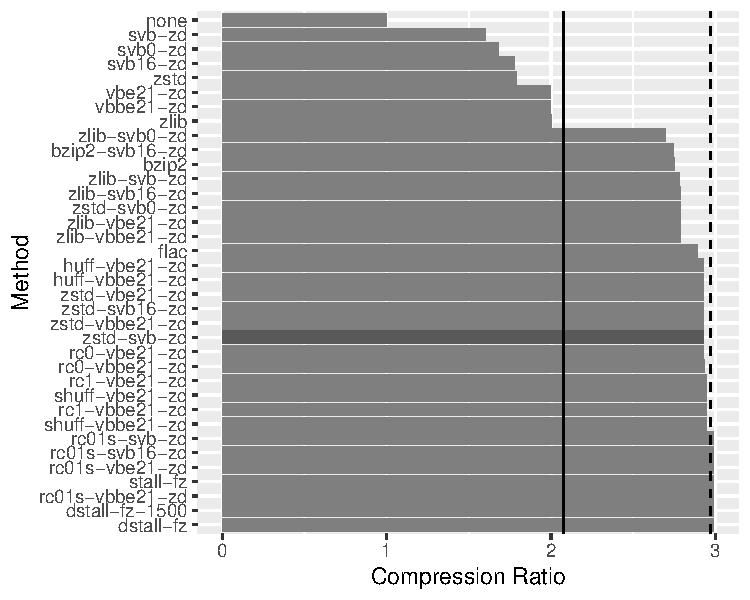
\includegraphics[scale=0.9]{plots/reads.blow5.test.ratio.bar.pdf}
	\caption[The compression ratio of each method on the
	data.]{\label{fig:results-ratio}The compression ratio of each method on the
	data. The state-of-the-art method is highlighted in a darker grey.
	The solid and dotted vertical lines represents the compression ratio
	equivalent of the entropy of the data and its deltas respectively.}
\end{figure}

\begin{figure}
\centering
%% Created by tikzDevice version 0.12.3.1 on 2022-11-04 11:04:58
% !TEX encoding = UTF-8 Unicode
\begin{tikzpicture}[x=1pt,y=0.95pt]
\definecolor{fillColor}{RGB}{255,255,255}
\path[use as bounding box,fill=fillColor,fill opacity=0.00] (0,0) rectangle (361.35,289.08);
\begin{scope}
\path[clip] (  0.00,  0.00) rectangle (361.35,289.08);
\definecolor{drawColor}{RGB}{255,255,255}
\definecolor{fillColor}{RGB}{255,255,255}

\path[draw=drawColor,line width= 0.6pt,line join=round,line cap=round,fill=fillColor] (  0.00,  0.00) rectangle (361.35,289.08);
\end{scope}
\begin{scope}
\path[clip] ( 84.57, 30.69) rectangle (355.85,283.58);
\definecolor{fillColor}{gray}{0.92}

\path[fill=fillColor] ( 84.57, 30.69) rectangle (355.85,283.58);
\definecolor{drawColor}{RGB}{255,255,255}

\path[draw=drawColor,line width= 0.3pt,line join=round] (133.95, 30.69) --
	(133.95,283.58);

\path[draw=drawColor,line width= 0.3pt,line join=round] (208.03, 30.69) --
	(208.03,283.58);

\path[draw=drawColor,line width= 0.3pt,line join=round] (282.12, 30.69) --
	(282.12,283.58);

\path[draw=drawColor,line width= 0.6pt,line join=round] ( 84.57, 34.88) --
	(355.85, 34.88);

\path[draw=drawColor,line width= 0.6pt,line join=round] ( 84.57, 41.86) --
	(355.85, 41.86);

\path[draw=drawColor,line width= 0.6pt,line join=round] ( 84.57, 48.85) --
	(355.85, 48.85);

\path[draw=drawColor,line width= 0.6pt,line join=round] ( 84.57, 55.84) --
	(355.85, 55.84);

\path[draw=drawColor,line width= 0.6pt,line join=round] ( 84.57, 62.82) --
	(355.85, 62.82);

\path[draw=drawColor,line width= 0.6pt,line join=round] ( 84.57, 69.81) --
	(355.85, 69.81);

\path[draw=drawColor,line width= 0.6pt,line join=round] ( 84.57, 76.79) --
	(355.85, 76.79);

\path[draw=drawColor,line width= 0.6pt,line join=round] ( 84.57, 83.78) --
	(355.85, 83.78);

\path[draw=drawColor,line width= 0.6pt,line join=round] ( 84.57, 90.77) --
	(355.85, 90.77);

\path[draw=drawColor,line width= 0.6pt,line join=round] ( 84.57, 97.75) --
	(355.85, 97.75);

\path[draw=drawColor,line width= 0.6pt,line join=round] ( 84.57,104.74) --
	(355.85,104.74);

\path[draw=drawColor,line width= 0.6pt,line join=round] ( 84.57,111.72) --
	(355.85,111.72);

\path[draw=drawColor,line width= 0.6pt,line join=round] ( 84.57,118.71) --
	(355.85,118.71);

\path[draw=drawColor,line width= 0.6pt,line join=round] ( 84.57,125.70) --
	(355.85,125.70);

\path[draw=drawColor,line width= 0.6pt,line join=round] ( 84.57,132.68) --
	(355.85,132.68);

\path[draw=drawColor,line width= 0.6pt,line join=round] ( 84.57,139.67) --
	(355.85,139.67);

\path[draw=drawColor,line width= 0.6pt,line join=round] ( 84.57,146.65) --
	(355.85,146.65);

\path[draw=drawColor,line width= 0.6pt,line join=round] ( 84.57,153.64) --
	(355.85,153.64);

\path[draw=drawColor,line width= 0.6pt,line join=round] ( 84.57,160.63) --
	(355.85,160.63);

\path[draw=drawColor,line width= 0.6pt,line join=round] ( 84.57,167.61) --
	(355.85,167.61);

\path[draw=drawColor,line width= 0.6pt,line join=round] ( 84.57,174.60) --
	(355.85,174.60);

\path[draw=drawColor,line width= 0.6pt,line join=round] ( 84.57,181.58) --
	(355.85,181.58);

\path[draw=drawColor,line width= 0.6pt,line join=round] ( 84.57,188.57) --
	(355.85,188.57);

\path[draw=drawColor,line width= 0.6pt,line join=round] ( 84.57,195.56) --
	(355.85,195.56);

\path[draw=drawColor,line width= 0.6pt,line join=round] ( 84.57,202.54) --
	(355.85,202.54);

\path[draw=drawColor,line width= 0.6pt,line join=round] ( 84.57,209.53) --
	(355.85,209.53);

\path[draw=drawColor,line width= 0.6pt,line join=round] ( 84.57,216.51) --
	(355.85,216.51);

\path[draw=drawColor,line width= 0.6pt,line join=round] ( 84.57,223.50) --
	(355.85,223.50);

\path[draw=drawColor,line width= 0.6pt,line join=round] ( 84.57,230.49) --
	(355.85,230.49);

\path[draw=drawColor,line width= 0.6pt,line join=round] ( 84.57,237.47) --
	(355.85,237.47);

\path[draw=drawColor,line width= 0.6pt,line join=round] ( 84.57,244.46) --
	(355.85,244.46);

\path[draw=drawColor,line width= 0.6pt,line join=round] ( 84.57,251.44) --
	(355.85,251.44);

\path[draw=drawColor,line width= 0.6pt,line join=round] ( 84.57,258.43) --
	(355.85,258.43);

\path[draw=drawColor,line width= 0.6pt,line join=round] ( 84.57,265.42) --
	(355.85,265.42);

\path[draw=drawColor,line width= 0.6pt,line join=round] ( 84.57,272.40) --
	(355.85,272.40);

\path[draw=drawColor,line width= 0.6pt,line join=round] ( 84.57,279.39) --
	(355.85,279.39);

\path[draw=drawColor,line width= 0.6pt,line join=round] ( 96.90, 30.69) --
	( 96.90,283.58);

\path[draw=drawColor,line width= 0.6pt,line join=round] (170.99, 30.69) --
	(170.99,283.58);

\path[draw=drawColor,line width= 0.6pt,line join=round] (245.08, 30.69) --
	(245.08,283.58);

\path[draw=drawColor,line width= 0.6pt,line join=round] (319.16, 30.69) --
	(319.16,283.58);
\definecolor{fillColor}{gray}{0.50}

\path[fill=fillColor] ( 96.90,276.24) rectangle ( 96.90,282.53);

\path[fill=fillColor] ( 96.90,227.34) rectangle (282.26,233.63);

\path[fill=fillColor] ( 96.90,248.30) rectangle (260.50,254.59);

\path[fill=fillColor] ( 96.90,206.38) rectangle (332.64,212.67);

\path[fill=fillColor] ( 96.90,269.26) rectangle (235.81,275.55);

\path[fill=fillColor] ( 96.90,255.29) rectangle (258.96,261.57);

\path[fill=fillColor] ( 96.90,262.27) rectangle (247.18,268.56);

\path[fill=fillColor] ( 96.90,241.31) rectangle (282.08,247.60);

\path[fill=fillColor] ( 96.90,234.33) rectangle (282.09,240.62);
\definecolor{fillColor}{gray}{0.35}

\path[fill=fillColor] ( 96.90,122.55) rectangle (340.84,128.84);
\definecolor{fillColor}{gray}{0.50}

\path[fill=fillColor] ( 96.90,136.52) rectangle (340.84,142.81);

\path[fill=fillColor] ( 96.90,185.43) rectangle (334.56,191.71);

\path[fill=fillColor] ( 96.90,143.51) rectangle (340.83,149.80);

\path[fill=fillColor] ( 96.90,129.54) rectangle (340.84,135.83);

\path[fill=fillColor] ( 96.90,199.40) rectangle (334.26,205.69);

\path[fill=fillColor] ( 96.90,192.41) rectangle (334.38,198.70);

\path[fill=fillColor] ( 96.90,220.36) rectangle (330.00,226.64);

\path[fill=fillColor] ( 96.90,178.44) rectangle (334.58,184.73);

\path[fill=fillColor] ( 96.90,171.45) rectangle (334.59,177.74);

\path[fill=fillColor] ( 96.90,213.37) rectangle (332.27,219.66);

\path[fill=fillColor] ( 96.90,164.47) rectangle (339.31,170.76);

\path[fill=fillColor] ( 96.90,157.48) rectangle (340.79,163.77);

\path[fill=fillColor] ( 96.90, 94.61) rectangle (341.67,100.90);

\path[fill=fillColor] ( 96.90,115.57) rectangle (340.94,121.85);

\path[fill=fillColor] ( 96.90,101.59) rectangle (341.66,107.88);

\path[fill=fillColor] ( 96.90, 59.68) rectangle (343.48, 65.97);

\path[fill=fillColor] ( 96.90,150.50) rectangle (340.81,156.78);

\path[fill=fillColor] ( 96.90, 80.64) rectangle (341.69, 86.92);

\path[fill=fillColor] ( 96.90,108.58) rectangle (340.96,114.87);

\path[fill=fillColor] ( 96.90, 87.62) rectangle (341.68, 93.91);

\path[fill=fillColor] ( 96.90, 45.71) rectangle (343.50, 51.99);

\path[fill=fillColor] ( 96.90, 52.69) rectangle (343.49, 58.98);

\path[fill=fillColor] ( 96.90, 73.65) rectangle (343.47, 79.94);

\path[fill=fillColor] ( 96.90, 66.66) rectangle (343.47, 72.95);

\path[fill=fillColor] ( 96.90, 31.73) rectangle (343.52, 38.02);

\path[fill=fillColor] ( 96.90, 38.72) rectangle (343.52, 45.01);
\definecolor{drawColor}{RGB}{0,0,0}

\path[draw=drawColor,line width= 0.6pt,line join=round] (289.07, 30.69) -- (289.07,283.58);

\path[draw=drawColor,line width= 0.6pt,dash pattern=on 4pt off 4pt ,line join=round] (342.55, 30.69) -- (342.55,283.58);
\end{scope}
\begin{scope}
\path[clip] (  0.00,  0.00) rectangle (361.35,289.08);
\definecolor{drawColor}{gray}{0.30}

\node[text=drawColor,anchor=base east,inner sep=0pt, outer sep=0pt, scale=  0.80] at ( 79.62, 31.85) {dstall-fz};

\node[text=drawColor,anchor=base east,inner sep=0pt, outer sep=0pt, scale=  0.80] at ( 79.62, 38.83) {dstall-fz-1500};

\node[text=drawColor,anchor=base east,inner sep=0pt, outer sep=0pt, scale=  0.80] at ( 79.62, 45.82) {rc01s-vbbe21-zd};

\node[text=drawColor,anchor=base east,inner sep=0pt, outer sep=0pt, scale=  0.80] at ( 79.62, 52.81) {stall-fz};

\node[text=drawColor,anchor=base east,inner sep=0pt, outer sep=0pt, scale=  0.80] at ( 79.62, 59.79) {rc01s-vbe21-zd};

\node[text=drawColor,anchor=base east,inner sep=0pt, outer sep=0pt, scale=  0.80] at ( 79.62, 66.78) {rc01s-svb16-zd};

\node[text=drawColor,anchor=base east,inner sep=0pt, outer sep=0pt, scale=  0.80] at ( 79.62, 73.76) {rc01s-svb-zd};

\node[text=drawColor,anchor=base east,inner sep=0pt, outer sep=0pt, scale=  0.80] at ( 79.62, 80.75) {shuff-vbbe21-zd};

\node[text=drawColor,anchor=base east,inner sep=0pt, outer sep=0pt, scale=  0.80] at ( 79.62, 87.74) {rc1-vbbe21-zd};

\node[text=drawColor,anchor=base east,inner sep=0pt, outer sep=0pt, scale=  0.80] at ( 79.62, 94.72) {shuff-vbe21-zd};

\node[text=drawColor,anchor=base east,inner sep=0pt, outer sep=0pt, scale=  0.80] at ( 79.62,101.71) {rc1-vbe21-zd};

\node[text=drawColor,anchor=base east,inner sep=0pt, outer sep=0pt, scale=  0.80] at ( 79.62,108.69) {rc0-vbbe21-zd};

\node[text=drawColor,anchor=base east,inner sep=0pt, outer sep=0pt, scale=  0.80] at ( 79.62,115.68) {rc0-vbe21-zd};

\node[text=drawColor,anchor=base east,inner sep=0pt, outer sep=0pt, scale=  0.80] at ( 79.62,122.67) {zstd-svb-zd};

\node[text=drawColor,anchor=base east,inner sep=0pt, outer sep=0pt, scale=  0.80] at ( 79.62,129.65) {zstd-vbbe21-zd};

\node[text=drawColor,anchor=base east,inner sep=0pt, outer sep=0pt, scale=  0.80] at ( 79.62,136.64) {zstd-svb16-zd};

\node[text=drawColor,anchor=base east,inner sep=0pt, outer sep=0pt, scale=  0.80] at ( 79.62,143.62) {zstd-vbe21-zd};

\node[text=drawColor,anchor=base east,inner sep=0pt, outer sep=0pt, scale=  0.80] at ( 79.62,150.61) {huff-vbbe21-zd};

\node[text=drawColor,anchor=base east,inner sep=0pt, outer sep=0pt, scale=  0.80] at ( 79.62,157.60) {huff-vbe21-zd};

\node[text=drawColor,anchor=base east,inner sep=0pt, outer sep=0pt, scale=  0.80] at ( 79.62,164.58) {flac};

\node[text=drawColor,anchor=base east,inner sep=0pt, outer sep=0pt, scale=  0.80] at ( 79.62,171.57) {zlib-vbbe21-zd};

\node[text=drawColor,anchor=base east,inner sep=0pt, outer sep=0pt, scale=  0.80] at ( 79.62,178.55) {zlib-vbe21-zd};

\node[text=drawColor,anchor=base east,inner sep=0pt, outer sep=0pt, scale=  0.80] at ( 79.62,185.54) {zstd-svb0-zd};

\node[text=drawColor,anchor=base east,inner sep=0pt, outer sep=0pt, scale=  0.80] at ( 79.62,192.53) {zlib-svb16-zd};

\node[text=drawColor,anchor=base east,inner sep=0pt, outer sep=0pt, scale=  0.80] at ( 79.62,199.51) {zlib-svb-zd};

\node[text=drawColor,anchor=base east,inner sep=0pt, outer sep=0pt, scale=  0.80] at ( 79.62,206.50) {bzip2};

\node[text=drawColor,anchor=base east,inner sep=0pt, outer sep=0pt, scale=  0.80] at ( 79.62,213.48) {bzip2-svb16-zd};

\node[text=drawColor,anchor=base east,inner sep=0pt, outer sep=0pt, scale=  0.80] at ( 79.62,220.47) {zlib-svb0-zd};

\node[text=drawColor,anchor=base east,inner sep=0pt, outer sep=0pt, scale=  0.80] at ( 79.62,227.46) {zlib};

\node[text=drawColor,anchor=base east,inner sep=0pt, outer sep=0pt, scale=  0.80] at ( 79.62,234.44) {vbbe21-zd};

\node[text=drawColor,anchor=base east,inner sep=0pt, outer sep=0pt, scale=  0.80] at ( 79.62,241.43) {vbe21-zd};

\node[text=drawColor,anchor=base east,inner sep=0pt, outer sep=0pt, scale=  0.80] at ( 79.62,248.41) {zstd};

\node[text=drawColor,anchor=base east,inner sep=0pt, outer sep=0pt, scale=  0.80] at ( 79.62,255.40) {svb16-zd};

\node[text=drawColor,anchor=base east,inner sep=0pt, outer sep=0pt, scale=  0.80] at ( 79.62,262.39) {svb0-zd};

\node[text=drawColor,anchor=base east,inner sep=0pt, outer sep=0pt, scale=  0.80] at ( 79.62,269.37) {svb-zd};

\node[text=drawColor,anchor=base east,inner sep=0pt, outer sep=0pt, scale=  0.80] at ( 79.62,276.36) {none};
\end{scope}
\begin{scope}
\path[clip] (  0.00,  0.00) rectangle (361.35,289.08);
\definecolor{drawColor}{gray}{0.20}

\path[draw=drawColor,line width= 0.6pt,line join=round] ( 81.82, 34.88) --
	( 84.57, 34.88);

\path[draw=drawColor,line width= 0.6pt,line join=round] ( 81.82, 41.86) --
	( 84.57, 41.86);

\path[draw=drawColor,line width= 0.6pt,line join=round] ( 81.82, 48.85) --
	( 84.57, 48.85);

\path[draw=drawColor,line width= 0.6pt,line join=round] ( 81.82, 55.84) --
	( 84.57, 55.84);

\path[draw=drawColor,line width= 0.6pt,line join=round] ( 81.82, 62.82) --
	( 84.57, 62.82);

\path[draw=drawColor,line width= 0.6pt,line join=round] ( 81.82, 69.81) --
	( 84.57, 69.81);

\path[draw=drawColor,line width= 0.6pt,line join=round] ( 81.82, 76.79) --
	( 84.57, 76.79);

\path[draw=drawColor,line width= 0.6pt,line join=round] ( 81.82, 83.78) --
	( 84.57, 83.78);

\path[draw=drawColor,line width= 0.6pt,line join=round] ( 81.82, 90.77) --
	( 84.57, 90.77);

\path[draw=drawColor,line width= 0.6pt,line join=round] ( 81.82, 97.75) --
	( 84.57, 97.75);

\path[draw=drawColor,line width= 0.6pt,line join=round] ( 81.82,104.74) --
	( 84.57,104.74);

\path[draw=drawColor,line width= 0.6pt,line join=round] ( 81.82,111.72) --
	( 84.57,111.72);

\path[draw=drawColor,line width= 0.6pt,line join=round] ( 81.82,118.71) --
	( 84.57,118.71);

\path[draw=drawColor,line width= 0.6pt,line join=round] ( 81.82,125.70) --
	( 84.57,125.70);

\path[draw=drawColor,line width= 0.6pt,line join=round] ( 81.82,132.68) --
	( 84.57,132.68);

\path[draw=drawColor,line width= 0.6pt,line join=round] ( 81.82,139.67) --
	( 84.57,139.67);

\path[draw=drawColor,line width= 0.6pt,line join=round] ( 81.82,146.65) --
	( 84.57,146.65);

\path[draw=drawColor,line width= 0.6pt,line join=round] ( 81.82,153.64) --
	( 84.57,153.64);

\path[draw=drawColor,line width= 0.6pt,line join=round] ( 81.82,160.63) --
	( 84.57,160.63);

\path[draw=drawColor,line width= 0.6pt,line join=round] ( 81.82,167.61) --
	( 84.57,167.61);

\path[draw=drawColor,line width= 0.6pt,line join=round] ( 81.82,174.60) --
	( 84.57,174.60);

\path[draw=drawColor,line width= 0.6pt,line join=round] ( 81.82,181.58) --
	( 84.57,181.58);

\path[draw=drawColor,line width= 0.6pt,line join=round] ( 81.82,188.57) --
	( 84.57,188.57);

\path[draw=drawColor,line width= 0.6pt,line join=round] ( 81.82,195.56) --
	( 84.57,195.56);

\path[draw=drawColor,line width= 0.6pt,line join=round] ( 81.82,202.54) --
	( 84.57,202.54);

\path[draw=drawColor,line width= 0.6pt,line join=round] ( 81.82,209.53) --
	( 84.57,209.53);

\path[draw=drawColor,line width= 0.6pt,line join=round] ( 81.82,216.51) --
	( 84.57,216.51);

\path[draw=drawColor,line width= 0.6pt,line join=round] ( 81.82,223.50) --
	( 84.57,223.50);

\path[draw=drawColor,line width= 0.6pt,line join=round] ( 81.82,230.49) --
	( 84.57,230.49);

\path[draw=drawColor,line width= 0.6pt,line join=round] ( 81.82,237.47) --
	( 84.57,237.47);

\path[draw=drawColor,line width= 0.6pt,line join=round] ( 81.82,244.46) --
	( 84.57,244.46);

\path[draw=drawColor,line width= 0.6pt,line join=round] ( 81.82,251.44) --
	( 84.57,251.44);

\path[draw=drawColor,line width= 0.6pt,line join=round] ( 81.82,258.43) --
	( 84.57,258.43);

\path[draw=drawColor,line width= 0.6pt,line join=round] ( 81.82,265.42) --
	( 84.57,265.42);

\path[draw=drawColor,line width= 0.6pt,line join=round] ( 81.82,272.40) --
	( 84.57,272.40);

\path[draw=drawColor,line width= 0.6pt,line join=round] ( 81.82,279.39) --
	( 84.57,279.39);
\end{scope}
\begin{scope}
\path[clip] (  0.00,  0.00) rectangle (361.35,289.08);
\definecolor{drawColor}{gray}{0.20}

\path[draw=drawColor,line width= 0.6pt,line join=round] ( 96.90, 27.94) --
	( 96.90, 30.69);

\path[draw=drawColor,line width= 0.6pt,line join=round] (170.99, 27.94) --
	(170.99, 30.69);

\path[draw=drawColor,line width= 0.6pt,line join=round] (245.08, 27.94) --
	(245.08, 30.69);

\path[draw=drawColor,line width= 0.6pt,line join=round] (319.16, 27.94) --
	(319.16, 30.69);
\end{scope}
\begin{scope}
\path[clip] (  0.00,  0.00) rectangle (361.35,289.08);
\definecolor{drawColor}{gray}{0.30}

\node[text=drawColor,anchor=base,inner sep=0pt, outer sep=0pt, scale=  0.80] at ( 96.90, 19.68) {0.0};

\node[text=drawColor,anchor=base,inner sep=0pt, outer sep=0pt, scale=  0.80] at (170.99, 19.68) {0.2};

\node[text=drawColor,anchor=base,inner sep=0pt, outer sep=0pt, scale=  0.80] at (245.08, 19.68) {0.4};

\node[text=drawColor,anchor=base,inner sep=0pt, outer sep=0pt, scale=  0.80] at (319.16, 19.68) {0.6};
\end{scope}
\begin{scope}
\path[clip] (  0.00,  0.00) rectangle (361.35,289.08);
\definecolor{drawColor}{RGB}{0,0,0}

\node[text=drawColor,anchor=base,inner sep=0pt, outer sep=0pt, scale=  1.10] at (220.21,  7.64) {Space Saving};
\end{scope}
\begin{scope}
\path[clip] (  0.00,  0.00) rectangle (361.35,289.08);
\definecolor{drawColor}{RGB}{0,0,0}

\node[text=drawColor,rotate= 90.00,anchor=base,inner sep=0pt, outer sep=0pt, scale=  1.10] at ( 13.08,157.13) {Method};
\end{scope}
\end{tikzpicture}

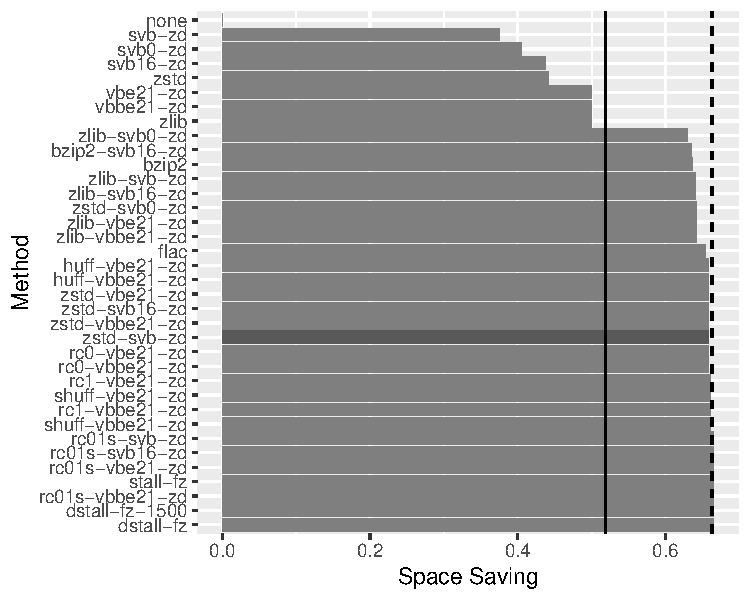
\includegraphics[scale=0.9]{plots/reads.blow5.test.ss.bar.pdf}
\caption{\label{fig:results-ss}The space saving of each method on the
	data. The state-of-the-art method is highlighted in a darker grey.
	The solid and dotted vertical lines represents the space saving
	equivalent of the entropy of the data and its deltas respectively.}
\end{figure}

\begin{figure}
\centering
%% Created by tikzDevice version 0.12.3.1 on 2022-11-04 11:24:38
% !TEX encoding = UTF-8 Unicode
\begin{tikzpicture}[x=1pt,y=0.80pt]
\definecolor{fillColor}{RGB}{255,255,255}
\path[use as bounding box,fill=fillColor,fill opacity=0.00] (0,0) rectangle (361.35,361.35);
\begin{scope}
\path[clip] (  0.00,  0.00) rectangle (361.35,361.35);
\definecolor{drawColor}{RGB}{255,255,255}
\definecolor{fillColor}{RGB}{255,255,255}

\path[draw=drawColor,line width= 0.6pt,line join=round,line cap=round,fill=fillColor] (  0.00,  0.00) rectangle (361.35,361.35);
\end{scope}
\begin{scope}
\path[clip] ( 84.57, 30.69) rectangle (355.85,330.66);
\definecolor{fillColor}{gray}{0.92}

\path[fill=fillColor] ( 84.57, 30.69) rectangle (355.85,330.66);
\definecolor{drawColor}{RGB}{255,255,255}

\path[draw=drawColor,line width= 0.3pt,line join=round] (135.44, 30.69) --
	(135.44,330.66);

\path[draw=drawColor,line width= 0.3pt,line join=round] (212.50, 30.69) --
	(212.50,330.66);

\path[draw=drawColor,line width= 0.3pt,line join=round] (289.57, 30.69) --
	(289.57,330.66);

\path[draw=drawColor,line width= 0.6pt,line join=round] ( 84.57, 35.66) --
	(355.85, 35.66);

\path[draw=drawColor,line width= 0.6pt,line join=round] ( 84.57, 43.94) --
	(355.85, 43.94);

\path[draw=drawColor,line width= 0.6pt,line join=round] ( 84.57, 52.23) --
	(355.85, 52.23);

\path[draw=drawColor,line width= 0.6pt,line join=round] ( 84.57, 60.52) --
	(355.85, 60.52);

\path[draw=drawColor,line width= 0.6pt,line join=round] ( 84.57, 68.80) --
	(355.85, 68.80);

\path[draw=drawColor,line width= 0.6pt,line join=round] ( 84.57, 77.09) --
	(355.85, 77.09);

\path[draw=drawColor,line width= 0.6pt,line join=round] ( 84.57, 85.38) --
	(355.85, 85.38);

\path[draw=drawColor,line width= 0.6pt,line join=round] ( 84.57, 93.66) --
	(355.85, 93.66);

\path[draw=drawColor,line width= 0.6pt,line join=round] ( 84.57,101.95) --
	(355.85,101.95);

\path[draw=drawColor,line width= 0.6pt,line join=round] ( 84.57,110.24) --
	(355.85,110.24);

\path[draw=drawColor,line width= 0.6pt,line join=round] ( 84.57,118.52) --
	(355.85,118.52);

\path[draw=drawColor,line width= 0.6pt,line join=round] ( 84.57,126.81) --
	(355.85,126.81);

\path[draw=drawColor,line width= 0.6pt,line join=round] ( 84.57,135.10) --
	(355.85,135.10);

\path[draw=drawColor,line width= 0.6pt,line join=round] ( 84.57,143.38) --
	(355.85,143.38);

\path[draw=drawColor,line width= 0.6pt,line join=round] ( 84.57,151.67) --
	(355.85,151.67);

\path[draw=drawColor,line width= 0.6pt,line join=round] ( 84.57,159.96) --
	(355.85,159.96);

\path[draw=drawColor,line width= 0.6pt,line join=round] ( 84.57,168.24) --
	(355.85,168.24);

\path[draw=drawColor,line width= 0.6pt,line join=round] ( 84.57,176.53) --
	(355.85,176.53);

\path[draw=drawColor,line width= 0.6pt,line join=round] ( 84.57,184.82) --
	(355.85,184.82);

\path[draw=drawColor,line width= 0.6pt,line join=round] ( 84.57,193.11) --
	(355.85,193.11);

\path[draw=drawColor,line width= 0.6pt,line join=round] ( 84.57,201.39) --
	(355.85,201.39);

\path[draw=drawColor,line width= 0.6pt,line join=round] ( 84.57,209.68) --
	(355.85,209.68);

\path[draw=drawColor,line width= 0.6pt,line join=round] ( 84.57,217.97) --
	(355.85,217.97);

\path[draw=drawColor,line width= 0.6pt,line join=round] ( 84.57,226.25) --
	(355.85,226.25);

\path[draw=drawColor,line width= 0.6pt,line join=round] ( 84.57,234.54) --
	(355.85,234.54);

\path[draw=drawColor,line width= 0.6pt,line join=round] ( 84.57,242.83) --
	(355.85,242.83);

\path[draw=drawColor,line width= 0.6pt,line join=round] ( 84.57,251.11) --
	(355.85,251.11);

\path[draw=drawColor,line width= 0.6pt,line join=round] ( 84.57,259.40) --
	(355.85,259.40);

\path[draw=drawColor,line width= 0.6pt,line join=round] ( 84.57,267.69) --
	(355.85,267.69);

\path[draw=drawColor,line width= 0.6pt,line join=round] ( 84.57,275.97) --
	(355.85,275.97);

\path[draw=drawColor,line width= 0.6pt,line join=round] ( 84.57,284.26) --
	(355.85,284.26);

\path[draw=drawColor,line width= 0.6pt,line join=round] ( 84.57,292.55) --
	(355.85,292.55);

\path[draw=drawColor,line width= 0.6pt,line join=round] ( 84.57,300.83) --
	(355.85,300.83);

\path[draw=drawColor,line width= 0.6pt,line join=round] ( 84.57,309.12) --
	(355.85,309.12);

\path[draw=drawColor,line width= 0.6pt,line join=round] ( 84.57,317.41) --
	(355.85,317.41);

\path[draw=drawColor,line width= 0.6pt,line join=round] ( 84.57,325.69) --
	(355.85,325.69);

\path[draw=drawColor,line width= 0.6pt,line join=round] ( 96.90, 30.69) --
	( 96.90,330.66);

\path[draw=drawColor,line width= 0.6pt,line join=round] (173.97, 30.69) --
	(173.97,330.66);

\path[draw=drawColor,line width= 0.6pt,line join=round] (251.04, 30.69) --
	(251.04,330.66);

\path[draw=drawColor,line width= 0.6pt,line join=round] (328.10, 30.69) --
	(328.10,330.66);
\definecolor{fillColor}{gray}{0.50}

\path[fill=fillColor] ( 96.90,321.96) rectangle (343.52,329.42);

\path[fill=fillColor] ( 96.90,263.96) rectangle (220.12,271.41);

\path[fill=fillColor] ( 96.90,288.82) rectangle (234.61,296.27);

\path[fill=fillColor] ( 96.90,239.10) rectangle (186.58,246.55);

\path[fill=fillColor] ( 96.90,313.68) rectangle (251.05,321.13);

\path[fill=fillColor] ( 96.90,297.10) rectangle (235.63,304.56);

\path[fill=fillColor] ( 96.90,305.39) rectangle (243.48,312.85);

\path[fill=fillColor] ( 96.90,280.53) rectangle (220.24,287.99);

\path[fill=fillColor] ( 96.90,272.24) rectangle (220.23,279.70);
\definecolor{fillColor}{gray}{0.35}

\path[fill=fillColor] ( 96.90,139.66) rectangle (181.12,147.11);
\definecolor{fillColor}{gray}{0.50}

\path[fill=fillColor] ( 96.90,156.23) rectangle (181.12,163.69);

\path[fill=fillColor] ( 96.90,214.24) rectangle (185.30,221.69);

\path[fill=fillColor] ( 96.90,164.52) rectangle (181.13,171.97);

\path[fill=fillColor] ( 96.90,147.94) rectangle (181.12,155.40);

\path[fill=fillColor] ( 96.90,230.81) rectangle (185.50,238.27);

\path[fill=fillColor] ( 96.90,222.52) rectangle (185.42,229.98);

\path[fill=fillColor] ( 96.90,255.67) rectangle (188.34,263.13);

\path[fill=fillColor] ( 96.90,205.95) rectangle (185.29,213.41);

\path[fill=fillColor] ( 96.90,197.66) rectangle (185.28,205.12);

\path[fill=fillColor] ( 96.90,247.38) rectangle (186.82,254.84);

\path[fill=fillColor] ( 96.90,189.38) rectangle (182.14,196.83);

\path[fill=fillColor] ( 96.90,181.09) rectangle (181.15,188.55);

\path[fill=fillColor] ( 96.90,106.51) rectangle (180.57,113.97);

\path[fill=fillColor] ( 96.90,131.37) rectangle (181.05,138.83);

\path[fill=fillColor] ( 96.90,114.80) rectangle (180.58,122.25);

\path[fill=fillColor] ( 96.90, 65.08) rectangle (179.36, 72.53);

\path[fill=fillColor] ( 96.90,172.80) rectangle (181.14,180.26);

\path[fill=fillColor] ( 96.90, 89.94) rectangle (180.55, 97.39);

\path[fill=fillColor] ( 96.90,123.08) rectangle (181.04,130.54);

\path[fill=fillColor] ( 96.90, 98.22) rectangle (180.56,105.68);

\path[fill=fillColor] ( 96.90, 48.50) rectangle (179.35, 55.96);

\path[fill=fillColor] ( 96.90, 56.79) rectangle (179.35, 64.25);

\path[fill=fillColor] ( 96.90, 81.65) rectangle (179.37, 89.11);

\path[fill=fillColor] ( 96.90, 73.36) rectangle (179.37, 80.82);

\path[fill=fillColor] ( 96.90, 31.93) rectangle (179.34, 39.39);

\path[fill=fillColor] ( 96.90, 40.22) rectangle (179.34, 47.67);
\definecolor{drawColor}{RGB}{0,0,0}

\path[draw=drawColor,line width= 0.6pt,line join=round] (215.59, 30.69) -- (215.59,330.66);

\path[draw=drawColor,line width= 0.6pt,dash pattern=on 4pt off 4pt ,line join=round] (179.98, 30.69) -- (179.98,330.66);
\end{scope}
\begin{scope}
\path[clip] (  0.00,  0.00) rectangle (361.35,361.35);
\definecolor{drawColor}{gray}{0.30}

\node[text=drawColor,anchor=base,inner sep=0pt, outer sep=0pt, scale=  0.80] at ( 96.79,335.61) {0};

\node[text=drawColor,anchor=base,inner sep=0pt, outer sep=0pt, scale=  0.80] at (155.18,335.61) {25};

\node[text=drawColor,anchor=base,inner sep=0pt, outer sep=0pt, scale=  0.80] at (213.56,335.61) {50};

\node[text=drawColor,anchor=base,inner sep=0pt, outer sep=0pt, scale=  0.80] at (271.94,335.61) {75};

\node[text=drawColor,anchor=base,inner sep=0pt, outer sep=0pt, scale=  0.80] at (330.32,335.61) {100};
\end{scope}
\begin{scope}
\path[clip] (  0.00,  0.00) rectangle (361.35,361.35);
\definecolor{drawColor}{gray}{0.20}

\path[draw=drawColor,line width= 0.6pt,line join=round] ( 96.79,330.66) --
	( 96.79,333.41);

\path[draw=drawColor,line width= 0.6pt,line join=round] (155.18,330.66) --
	(155.18,333.41);

\path[draw=drawColor,line width= 0.6pt,line join=round] (213.56,330.66) --
	(213.56,333.41);

\path[draw=drawColor,line width= 0.6pt,line join=round] (271.94,330.66) --
	(271.94,333.41);

\path[draw=drawColor,line width= 0.6pt,line join=round] (330.32,330.66) --
	(330.32,333.41);
\end{scope}
\begin{scope}
\path[clip] (  0.00,  0.00) rectangle (361.35,361.35);
\definecolor{drawColor}{gray}{0.30}

\node[text=drawColor,anchor=base east,inner sep=0pt, outer sep=0pt, scale=  0.80] at ( 79.62, 32.63) {dstall-fz};

\node[text=drawColor,anchor=base east,inner sep=0pt, outer sep=0pt, scale=  0.80] at ( 79.62, 40.91) {dstall-fz-1500};

\node[text=drawColor,anchor=base east,inner sep=0pt, outer sep=0pt, scale=  0.80] at ( 79.62, 49.20) {rc01s-vbbe21-zd};

\node[text=drawColor,anchor=base east,inner sep=0pt, outer sep=0pt, scale=  0.80] at ( 79.62, 57.49) {stall-fz};

\node[text=drawColor,anchor=base east,inner sep=0pt, outer sep=0pt, scale=  0.80] at ( 79.62, 65.77) {rc01s-vbe21-zd};

\node[text=drawColor,anchor=base east,inner sep=0pt, outer sep=0pt, scale=  0.80] at ( 79.62, 74.06) {rc01s-svb16-zd};

\node[text=drawColor,anchor=base east,inner sep=0pt, outer sep=0pt, scale=  0.80] at ( 79.62, 82.35) {rc01s-svb-zd};

\node[text=drawColor,anchor=base east,inner sep=0pt, outer sep=0pt, scale=  0.80] at ( 79.62, 90.63) {shuff-vbbe21-zd};

\node[text=drawColor,anchor=base east,inner sep=0pt, outer sep=0pt, scale=  0.80] at ( 79.62, 98.92) {rc1-vbbe21-zd};

\node[text=drawColor,anchor=base east,inner sep=0pt, outer sep=0pt, scale=  0.80] at ( 79.62,107.21) {shuff-vbe21-zd};

\node[text=drawColor,anchor=base east,inner sep=0pt, outer sep=0pt, scale=  0.80] at ( 79.62,115.49) {rc1-vbe21-zd};

\node[text=drawColor,anchor=base east,inner sep=0pt, outer sep=0pt, scale=  0.80] at ( 79.62,123.78) {rc0-vbbe21-zd};

\node[text=drawColor,anchor=base east,inner sep=0pt, outer sep=0pt, scale=  0.80] at ( 79.62,132.07) {rc0-vbe21-zd};

\node[text=drawColor,anchor=base east,inner sep=0pt, outer sep=0pt, scale=  0.80] at ( 79.62,140.35) {zstd-svb-zd};

\node[text=drawColor,anchor=base east,inner sep=0pt, outer sep=0pt, scale=  0.80] at ( 79.62,148.64) {zstd-vbbe21-zd};

\node[text=drawColor,anchor=base east,inner sep=0pt, outer sep=0pt, scale=  0.80] at ( 79.62,156.93) {zstd-svb16-zd};

\node[text=drawColor,anchor=base east,inner sep=0pt, outer sep=0pt, scale=  0.80] at ( 79.62,165.21) {zstd-vbe21-zd};

\node[text=drawColor,anchor=base east,inner sep=0pt, outer sep=0pt, scale=  0.80] at ( 79.62,173.50) {huff-vbbe21-zd};

\node[text=drawColor,anchor=base east,inner sep=0pt, outer sep=0pt, scale=  0.80] at ( 79.62,181.79) {huff-vbe21-zd};

\node[text=drawColor,anchor=base east,inner sep=0pt, outer sep=0pt, scale=  0.80] at ( 79.62,190.07) {flac};

\node[text=drawColor,anchor=base east,inner sep=0pt, outer sep=0pt, scale=  0.80] at ( 79.62,198.36) {zlib-vbbe21-zd};

\node[text=drawColor,anchor=base east,inner sep=0pt, outer sep=0pt, scale=  0.80] at ( 79.62,206.65) {zlib-vbe21-zd};

\node[text=drawColor,anchor=base east,inner sep=0pt, outer sep=0pt, scale=  0.80] at ( 79.62,214.93) {zstd-svb0-zd};

\node[text=drawColor,anchor=base east,inner sep=0pt, outer sep=0pt, scale=  0.80] at ( 79.62,223.22) {zlib-svb16-zd};

\node[text=drawColor,anchor=base east,inner sep=0pt, outer sep=0pt, scale=  0.80] at ( 79.62,231.51) {zlib-svb-zd};

\node[text=drawColor,anchor=base east,inner sep=0pt, outer sep=0pt, scale=  0.80] at ( 79.62,239.79) {bzip2};

\node[text=drawColor,anchor=base east,inner sep=0pt, outer sep=0pt, scale=  0.80] at ( 79.62,248.08) {bzip2-svb16-zd};

\node[text=drawColor,anchor=base east,inner sep=0pt, outer sep=0pt, scale=  0.80] at ( 79.62,256.37) {zlib-svb0-zd};

\node[text=drawColor,anchor=base east,inner sep=0pt, outer sep=0pt, scale=  0.80] at ( 79.62,264.65) {zlib};

\node[text=drawColor,anchor=base east,inner sep=0pt, outer sep=0pt, scale=  0.80] at ( 79.62,272.94) {vbbe21-zd};

\node[text=drawColor,anchor=base east,inner sep=0pt, outer sep=0pt, scale=  0.80] at ( 79.62,281.23) {vbe21-zd};

\node[text=drawColor,anchor=base east,inner sep=0pt, outer sep=0pt, scale=  0.80] at ( 79.62,289.52) {zstd};

\node[text=drawColor,anchor=base east,inner sep=0pt, outer sep=0pt, scale=  0.80] at ( 79.62,297.80) {svb16-zd};

\node[text=drawColor,anchor=base east,inner sep=0pt, outer sep=0pt, scale=  0.80] at ( 79.62,306.09) {svb0-zd};

\node[text=drawColor,anchor=base east,inner sep=0pt, outer sep=0pt, scale=  0.80] at ( 79.62,314.38) {svb-zd};

\node[text=drawColor,anchor=base east,inner sep=0pt, outer sep=0pt, scale=  0.80] at ( 79.62,322.66) {none};
\end{scope}
\begin{scope}
\path[clip] (  0.00,  0.00) rectangle (361.35,361.35);
\definecolor{drawColor}{gray}{0.20}

\path[draw=drawColor,line width= 0.6pt,line join=round] ( 81.82, 35.66) --
	( 84.57, 35.66);

\path[draw=drawColor,line width= 0.6pt,line join=round] ( 81.82, 43.94) --
	( 84.57, 43.94);

\path[draw=drawColor,line width= 0.6pt,line join=round] ( 81.82, 52.23) --
	( 84.57, 52.23);

\path[draw=drawColor,line width= 0.6pt,line join=round] ( 81.82, 60.52) --
	( 84.57, 60.52);

\path[draw=drawColor,line width= 0.6pt,line join=round] ( 81.82, 68.80) --
	( 84.57, 68.80);

\path[draw=drawColor,line width= 0.6pt,line join=round] ( 81.82, 77.09) --
	( 84.57, 77.09);

\path[draw=drawColor,line width= 0.6pt,line join=round] ( 81.82, 85.38) --
	( 84.57, 85.38);

\path[draw=drawColor,line width= 0.6pt,line join=round] ( 81.82, 93.66) --
	( 84.57, 93.66);

\path[draw=drawColor,line width= 0.6pt,line join=round] ( 81.82,101.95) --
	( 84.57,101.95);

\path[draw=drawColor,line width= 0.6pt,line join=round] ( 81.82,110.24) --
	( 84.57,110.24);

\path[draw=drawColor,line width= 0.6pt,line join=round] ( 81.82,118.52) --
	( 84.57,118.52);

\path[draw=drawColor,line width= 0.6pt,line join=round] ( 81.82,126.81) --
	( 84.57,126.81);

\path[draw=drawColor,line width= 0.6pt,line join=round] ( 81.82,135.10) --
	( 84.57,135.10);

\path[draw=drawColor,line width= 0.6pt,line join=round] ( 81.82,143.38) --
	( 84.57,143.38);

\path[draw=drawColor,line width= 0.6pt,line join=round] ( 81.82,151.67) --
	( 84.57,151.67);

\path[draw=drawColor,line width= 0.6pt,line join=round] ( 81.82,159.96) --
	( 84.57,159.96);

\path[draw=drawColor,line width= 0.6pt,line join=round] ( 81.82,168.24) --
	( 84.57,168.24);

\path[draw=drawColor,line width= 0.6pt,line join=round] ( 81.82,176.53) --
	( 84.57,176.53);

\path[draw=drawColor,line width= 0.6pt,line join=round] ( 81.82,184.82) --
	( 84.57,184.82);

\path[draw=drawColor,line width= 0.6pt,line join=round] ( 81.82,193.11) --
	( 84.57,193.11);

\path[draw=drawColor,line width= 0.6pt,line join=round] ( 81.82,201.39) --
	( 84.57,201.39);

\path[draw=drawColor,line width= 0.6pt,line join=round] ( 81.82,209.68) --
	( 84.57,209.68);

\path[draw=drawColor,line width= 0.6pt,line join=round] ( 81.82,217.97) --
	( 84.57,217.97);

\path[draw=drawColor,line width= 0.6pt,line join=round] ( 81.82,226.25) --
	( 84.57,226.25);

\path[draw=drawColor,line width= 0.6pt,line join=round] ( 81.82,234.54) --
	( 84.57,234.54);

\path[draw=drawColor,line width= 0.6pt,line join=round] ( 81.82,242.83) --
	( 84.57,242.83);

\path[draw=drawColor,line width= 0.6pt,line join=round] ( 81.82,251.11) --
	( 84.57,251.11);

\path[draw=drawColor,line width= 0.6pt,line join=round] ( 81.82,259.40) --
	( 84.57,259.40);

\path[draw=drawColor,line width= 0.6pt,line join=round] ( 81.82,267.69) --
	( 84.57,267.69);

\path[draw=drawColor,line width= 0.6pt,line join=round] ( 81.82,275.97) --
	( 84.57,275.97);

\path[draw=drawColor,line width= 0.6pt,line join=round] ( 81.82,284.26) --
	( 84.57,284.26);

\path[draw=drawColor,line width= 0.6pt,line join=round] ( 81.82,292.55) --
	( 84.57,292.55);

\path[draw=drawColor,line width= 0.6pt,line join=round] ( 81.82,300.83) --
	( 84.57,300.83);

\path[draw=drawColor,line width= 0.6pt,line join=round] ( 81.82,309.12) --
	( 84.57,309.12);

\path[draw=drawColor,line width= 0.6pt,line join=round] ( 81.82,317.41) --
	( 84.57,317.41);

\path[draw=drawColor,line width= 0.6pt,line join=round] ( 81.82,325.69) --
	( 84.57,325.69);
\end{scope}
\begin{scope}
\path[clip] (  0.00,  0.00) rectangle (361.35,361.35);
\definecolor{drawColor}{gray}{0.20}

\path[draw=drawColor,line width= 0.6pt,line join=round] ( 96.90, 27.94) --
	( 96.90, 30.69);

\path[draw=drawColor,line width= 0.6pt,line join=round] (173.97, 27.94) --
	(173.97, 30.69);

\path[draw=drawColor,line width= 0.6pt,line join=round] (251.04, 27.94) --
	(251.04, 30.69);

\path[draw=drawColor,line width= 0.6pt,line join=round] (328.10, 27.94) --
	(328.10, 30.69);
\end{scope}
\begin{scope}
\path[clip] (  0.00,  0.00) rectangle (361.35,361.35);
\definecolor{drawColor}{gray}{0.30}

\node[text=drawColor,anchor=base,inner sep=0pt, outer sep=0pt, scale=  0.80] at ( 96.90, 19.68) {0};

\node[text=drawColor,anchor=base,inner sep=0pt, outer sep=0pt, scale=  0.80] at (173.97, 19.68) {5};

\node[text=drawColor,anchor=base,inner sep=0pt, outer sep=0pt, scale=  0.80] at (251.04, 19.68) {10};

\node[text=drawColor,anchor=base,inner sep=0pt, outer sep=0pt, scale=  0.80] at (328.10, 19.68) {15};
\end{scope}
\begin{scope}
\path[clip] (  0.00,  0.00) rectangle (361.35,361.35);
\definecolor{drawColor}{RGB}{0,0,0}

\node[text=drawColor,anchor=base,inner sep=0pt, outer sep=0pt, scale=  1.10] at (220.21,346.14) {Compressed Size (GiB)};
\end{scope}
\begin{scope}
\path[clip] (  0.00,  0.00) rectangle (361.35,361.35);
\definecolor{drawColor}{RGB}{0,0,0}

\node[text=drawColor,anchor=base,inner sep=0pt, outer sep=0pt, scale=  1.10] at (220.21,  7.64) {Bits per Symbol};
\end{scope}
\begin{scope}
\path[clip] (  0.00,  0.00) rectangle (361.35,361.35);
\definecolor{drawColor}{RGB}{0,0,0}

\node[text=drawColor,rotate= 90.00,anchor=base,inner sep=0pt, outer sep=0pt, scale=  1.10] at ( 13.08,180.68) {Method};
\end{scope}
\end{tikzpicture}

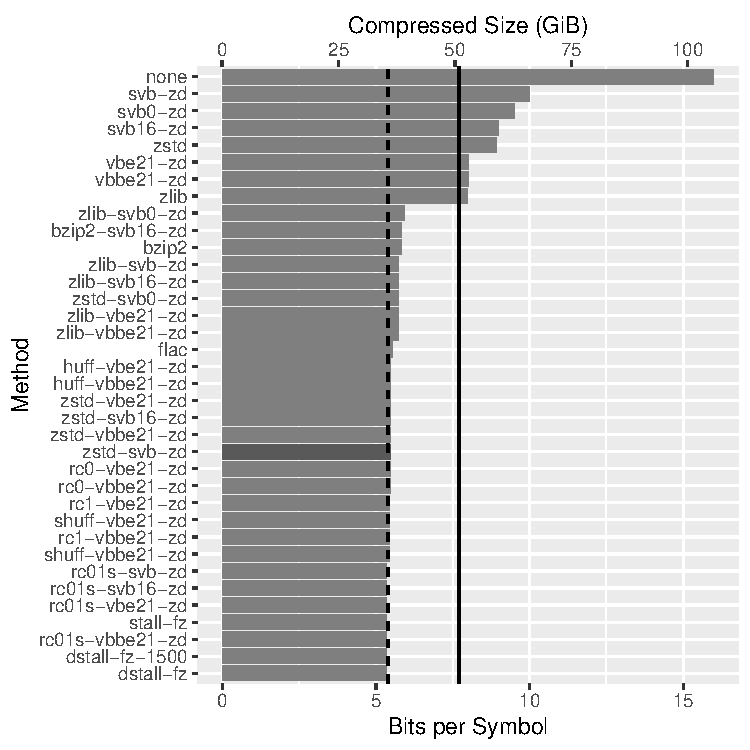
\includegraphics[scale=0.9]{plots/reads.blow5.test.bps.bar.pdf}
\caption{\label{fig:results-bps}The average number of bits used per symbol and
	total compressed size of each method on the data. The state-of-the-art
	method is highlighted in a darker grey. The solid and dotted vertical
	lines represents the bits per symbol equivalent of the entropy of the
	data and its deltas respectively.}
\end{figure}

\begin{figure}
\centering
%% Created by tikzDevice version 0.12.3.1 on 2022-11-04 11:05:01
% !TEX encoding = UTF-8 Unicode
\begin{tikzpicture}[x=1pt,y=0.95pt]
\definecolor{fillColor}{RGB}{255,255,255}
\path[use as bounding box,fill=fillColor,fill opacity=0.00] (0,0) rectangle (289.08,289.08);
\begin{scope}
\path[clip] (  0.00,  0.00) rectangle (289.08,289.08);
\definecolor{drawColor}{RGB}{255,255,255}
\definecolor{fillColor}{RGB}{255,255,255}

\path[draw=drawColor,line width= 0.6pt,line join=round,line cap=round,fill=fillColor] (  0.00,  0.00) rectangle (289.08,289.08);
\end{scope}
\begin{scope}
\path[clip] ( 31.71, 30.69) rectangle (283.58,283.58);
\definecolor{fillColor}{gray}{0.92}

\path[fill=fillColor] ( 31.71, 30.69) rectangle (283.58,283.58);
\definecolor{drawColor}{RGB}{255,255,255}

\path[draw=drawColor,line width= 0.3pt,line join=round] ( 31.71, 79.26) --
	(283.58, 79.26);

\path[draw=drawColor,line width= 0.3pt,line join=round] ( 31.71,153.43) --
	(283.58,153.43);

\path[draw=drawColor,line width= 0.3pt,line join=round] ( 31.71,227.60) --
	(283.58,227.60);

\path[draw=drawColor,line width= 0.3pt,line join=round] ( 77.55, 30.69) --
	( 77.55,283.58);

\path[draw=drawColor,line width= 0.3pt,line join=round] (146.34, 30.69) --
	(146.34,283.58);

\path[draw=drawColor,line width= 0.3pt,line join=round] (215.13, 30.69) --
	(215.13,283.58);

\path[draw=drawColor,line width= 0.6pt,line join=round] ( 31.71, 42.18) --
	(283.58, 42.18);

\path[draw=drawColor,line width= 0.6pt,line join=round] ( 31.71,116.35) --
	(283.58,116.35);

\path[draw=drawColor,line width= 0.6pt,line join=round] ( 31.71,190.51) --
	(283.58,190.51);

\path[draw=drawColor,line width= 0.6pt,line join=round] ( 31.71,264.68) --
	(283.58,264.68);

\path[draw=drawColor,line width= 0.6pt,line join=round] ( 43.16, 30.69) --
	( 43.16,283.58);

\path[draw=drawColor,line width= 0.6pt,line join=round] (111.95, 30.69) --
	(111.95,283.58);

\path[draw=drawColor,line width= 0.6pt,line join=round] (180.73, 30.69) --
	(180.73,283.58);

\path[draw=drawColor,line width= 0.6pt,line join=round] (249.52, 30.69) --
	(249.52,283.58);
\definecolor{drawColor}{gray}{0.50}
\definecolor{fillColor}{gray}{0.50}

\path[draw=drawColor,line width= 0.4pt,line join=round,line cap=round,fill=fillColor] ( 43.16, 42.18) circle (  1.96);

\path[draw=drawColor,line width= 0.4pt,line join=round,line cap=round,fill=fillColor] (215.25,252.78) circle (  1.96);

\path[draw=drawColor,line width= 0.4pt,line join=round,line cap=round,fill=fillColor] (195.05, 57.40) circle (  1.96);

\path[draw=drawColor,line width= 0.4pt,line join=round,line cap=round,fill=fillColor] (262.03,233.08) circle (  1.96);

\path[draw=drawColor,line width= 0.4pt,line join=round,line cap=round,fill=fillColor] (172.13, 47.66) circle (  1.96);

\path[draw=drawColor,line width= 0.4pt,line join=round,line cap=round,fill=fillColor] (193.62, 48.03) circle (  1.96);

\path[draw=drawColor,line width= 0.4pt,line join=round,line cap=round,fill=fillColor] (182.68, 48.37) circle (  1.96);

\path[draw=drawColor,line width= 0.4pt,line join=round,line cap=round,fill=fillColor] (215.09, 52.28) circle (  1.96);

\path[draw=drawColor,line width= 0.4pt,line join=round,line cap=round,fill=fillColor] (215.10, 55.89) circle (  1.96);
\definecolor{drawColor}{RGB}{255,0,0}
\definecolor{fillColor}{RGB}{255,0,0}

\path[draw=drawColor,line width= 0.4pt,line join=round,line cap=round,fill=fillColor] (269.65, 49.93) circle (  1.96);
\definecolor{drawColor}{gray}{0.50}
\definecolor{fillColor}{gray}{0.50}

\path[draw=drawColor,line width= 0.4pt,line join=round,line cap=round,fill=fillColor] (269.64, 50.24) circle (  1.96);

\path[draw=drawColor,line width= 0.4pt,line join=round,line cap=round,fill=fillColor] (263.81, 52.13) circle (  1.96);

\path[draw=drawColor,line width= 0.4pt,line join=round,line cap=round,fill=fillColor] (269.63, 54.44) circle (  1.96);

\path[draw=drawColor,line width= 0.4pt,line join=round,line cap=round,fill=fillColor] (269.65, 58.81) circle (  1.96);

\path[draw=drawColor,line width= 0.4pt,line join=round,line cap=round,fill=fillColor] (263.53,103.18) circle (  1.96);

\path[draw=drawColor,line width= 0.4pt,line join=round,line cap=round,fill=fillColor] (263.65,102.42) circle (  1.96);

\path[draw=drawColor,line width= 0.4pt,line join=round,line cap=round,fill=fillColor] (259.58,125.54) circle (  1.96);

\path[draw=drawColor,line width= 0.4pt,line join=round,line cap=round,fill=fillColor] (263.83,105.14) circle (  1.96);

\path[draw=drawColor,line width= 0.4pt,line join=round,line cap=round,fill=fillColor] (263.84,122.70) circle (  1.96);

\path[draw=drawColor,line width= 0.4pt,line join=round,line cap=round,fill=fillColor] (261.69,160.86) circle (  1.96);

\path[draw=drawColor,line width= 0.4pt,line join=round,line cap=round,fill=fillColor] (268.22, 72.98) circle (  1.96);

\path[draw=drawColor,line width= 0.4pt,line join=round,line cap=round,fill=fillColor] (269.60,126.24) circle (  1.96);

\path[draw=drawColor,line width= 0.4pt,line join=round,line cap=round,fill=fillColor] (270.42,108.81) circle (  1.96);

\path[draw=drawColor,line width= 0.4pt,line join=round,line cap=round,fill=fillColor] (269.74, 85.41) circle (  1.96);

\path[draw=drawColor,line width= 0.4pt,line join=round,line cap=round,fill=fillColor] (270.40, 85.28) circle (  1.96);

\path[draw=drawColor,line width= 0.4pt,line join=round,line cap=round,fill=fillColor] (272.10,159.58) circle (  1.96);

\path[draw=drawColor,line width= 0.4pt,line join=round,line cap=round,fill=fillColor] (269.62,131.13) circle (  1.96);

\path[draw=drawColor,line width= 0.4pt,line join=round,line cap=round,fill=fillColor] (270.43,109.48) circle (  1.96);

\path[draw=drawColor,line width= 0.4pt,line join=round,line cap=round,fill=fillColor] (269.75, 84.94) circle (  1.96);

\path[draw=drawColor,line width= 0.4pt,line join=round,line cap=round,fill=fillColor] (270.42, 86.35) circle (  1.96);

\path[draw=drawColor,line width= 0.4pt,line join=round,line cap=round,fill=fillColor] (272.12,158.53) circle (  1.96);

\path[draw=drawColor,line width= 0.4pt,line join=round,line cap=round,fill=fillColor] (272.11,162.86) circle (  1.96);

\path[draw=drawColor,line width= 0.4pt,line join=round,line cap=round,fill=fillColor] (272.08,175.41) circle (  1.96);

\path[draw=drawColor,line width= 0.4pt,line join=round,line cap=round,fill=fillColor] (272.09,159.13) circle (  1.96);

\path[draw=drawColor,line width= 0.4pt,line join=round,line cap=round,fill=fillColor] (272.13,272.08) circle (  1.96);

\path[draw=drawColor,line width= 0.4pt,line join=round,line cap=round,fill=fillColor] (272.13,162.28) circle (  1.96);

\path[draw=drawColor,line width= 0.6pt,line join=round,line cap=round] (265.79, 68.14) -- (269.54, 84.04);

\node[text=drawColor,anchor=base,inner sep=0pt, outer sep=0pt, scale=  1.10] at ( 50.88, 46.14) {none};

\node[text=drawColor,anchor=base,inner sep=0pt, outer sep=0pt, scale=  1.10] at (158.22, 36.13) {svb-zd};

\node[text=drawColor,anchor=base,inner sep=0pt, outer sep=0pt, scale=  1.10] at (200.76, 33.70) {svb16-zd};
\definecolor{drawColor}{RGB}{255,0,0}

\node[text=drawColor,anchor=base,inner sep=0pt, outer sep=0pt, scale=  1.10] at (253.37, 38.38) {zstd-svb-zd};
\definecolor{drawColor}{gray}{0.50}

\node[text=drawColor,anchor=base,inner sep=0pt, outer sep=0pt, scale=  1.10] at (233.88, 76.64) {rc1-vbe21-zd};

\node[text=drawColor,anchor=base,inner sep=0pt, outer sep=0pt, scale=  1.10] at (228.96,111.12) {shuff-vbbe21-zd};

\node[text=drawColor,anchor=base,inner sep=0pt, outer sep=0pt, scale=  1.10] at (230.55, 62.88) {rc0-vbbe21-zd};

\node[text=drawColor,anchor=base,inner sep=0pt, outer sep=0pt, scale=  1.10] at (246.83, 90.28) {rc1-vbbe21-zd};

\node[text=drawColor,anchor=base,inner sep=0pt, outer sep=0pt, scale=  1.10] at (241.86,147.01) {rc01s-vbbe21-zd};

\node[text=drawColor,anchor=base,inner sep=0pt, outer sep=0pt, scale=  1.10] at (249.05,268.28) {dstall-fz};

\node[text=drawColor,anchor=base,inner sep=0pt, outer sep=0pt, scale=  1.10] at (236.11,164.81) {dstall-fz-1500};
\end{scope}
\begin{scope}
\path[clip] (  0.00,  0.00) rectangle (289.08,289.08);
\definecolor{drawColor}{gray}{0.30}

\node[text=drawColor,anchor=base east,inner sep=0pt, outer sep=0pt, scale=  0.88] at ( 26.76, 39.15) {0};

\node[text=drawColor,anchor=base east,inner sep=0pt, outer sep=0pt, scale=  0.88] at ( 26.76,113.32) {10};

\node[text=drawColor,anchor=base east,inner sep=0pt, outer sep=0pt, scale=  0.88] at ( 26.76,187.48) {20};

\node[text=drawColor,anchor=base east,inner sep=0pt, outer sep=0pt, scale=  0.88] at ( 26.76,261.65) {30};
\end{scope}
\begin{scope}
\path[clip] (  0.00,  0.00) rectangle (289.08,289.08);
\definecolor{drawColor}{gray}{0.20}

\path[draw=drawColor,line width= 0.6pt,line join=round] ( 28.96, 42.18) --
	( 31.71, 42.18);

\path[draw=drawColor,line width= 0.6pt,line join=round] ( 28.96,116.35) --
	( 31.71,116.35);

\path[draw=drawColor,line width= 0.6pt,line join=round] ( 28.96,190.51) --
	( 31.71,190.51);

\path[draw=drawColor,line width= 0.6pt,line join=round] ( 28.96,264.68) --
	( 31.71,264.68);
\end{scope}
\begin{scope}
\path[clip] (  0.00,  0.00) rectangle (289.08,289.08);
\definecolor{drawColor}{gray}{0.20}

\path[draw=drawColor,line width= 0.6pt,line join=round] ( 43.16, 27.94) --
	( 43.16, 30.69);

\path[draw=drawColor,line width= 0.6pt,line join=round] (111.95, 27.94) --
	(111.95, 30.69);

\path[draw=drawColor,line width= 0.6pt,line join=round] (180.73, 27.94) --
	(180.73, 30.69);

\path[draw=drawColor,line width= 0.6pt,line join=round] (249.52, 27.94) --
	(249.52, 30.69);
\end{scope}
\begin{scope}
\path[clip] (  0.00,  0.00) rectangle (289.08,289.08);
\definecolor{drawColor}{gray}{0.30}

\node[text=drawColor,anchor=base,inner sep=0pt, outer sep=0pt, scale=  0.88] at ( 43.16, 19.68) {0.0};

\node[text=drawColor,anchor=base,inner sep=0pt, outer sep=0pt, scale=  0.88] at (111.95, 19.68) {0.2};

\node[text=drawColor,anchor=base,inner sep=0pt, outer sep=0pt, scale=  0.88] at (180.73, 19.68) {0.4};

\node[text=drawColor,anchor=base,inner sep=0pt, outer sep=0pt, scale=  0.88] at (249.52, 19.68) {0.6};
\end{scope}
\begin{scope}
\path[clip] (  0.00,  0.00) rectangle (289.08,289.08);
\definecolor{drawColor}{RGB}{0,0,0}

\node[text=drawColor,anchor=base,inner sep=0pt, outer sep=0pt, scale=  1.10] at (157.65,  7.64) {Space Saving};
\end{scope}
\begin{scope}
\path[clip] (  0.00,  0.00) rectangle (289.08,289.08);
\definecolor{drawColor}{RGB}{0,0,0}

\node[text=drawColor,rotate= 90.00,anchor=base,inner sep=0pt, outer sep=0pt, scale=  1.10] at ( 13.08,157.13) {Compression Time (hr / TiB)};
\end{scope}
\end{tikzpicture}

\subfloat[\label{fig:results-ss-ct-big}]{
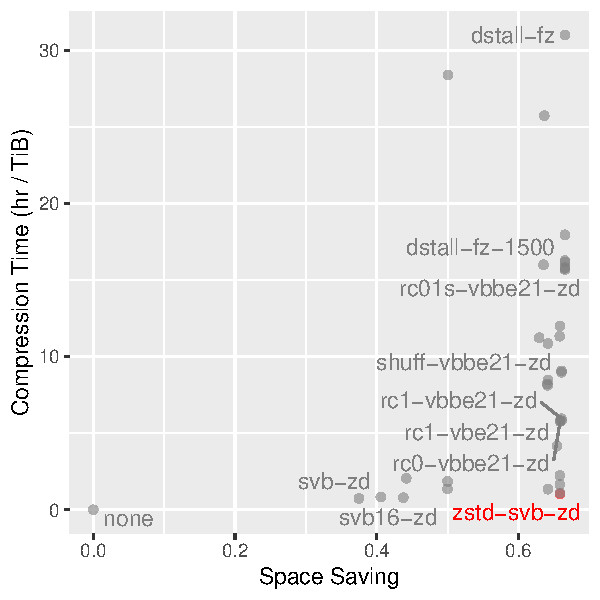
\includegraphics[scale=0.7,valign=t]{plots/reads.blow5.test.ss-ct.pdf}
}
\subfloat[\label{fig:results-ss-ct-small}]{
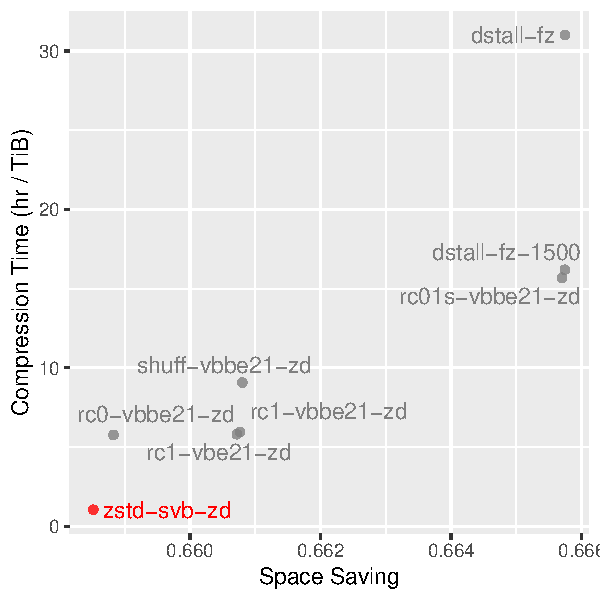
\includegraphics[scale=0.7,valign=t]{plots/reads.blow5.test.ss-ct06.pdf}
}

\subfloat[\label{fig:results-ss-dt-big}]{
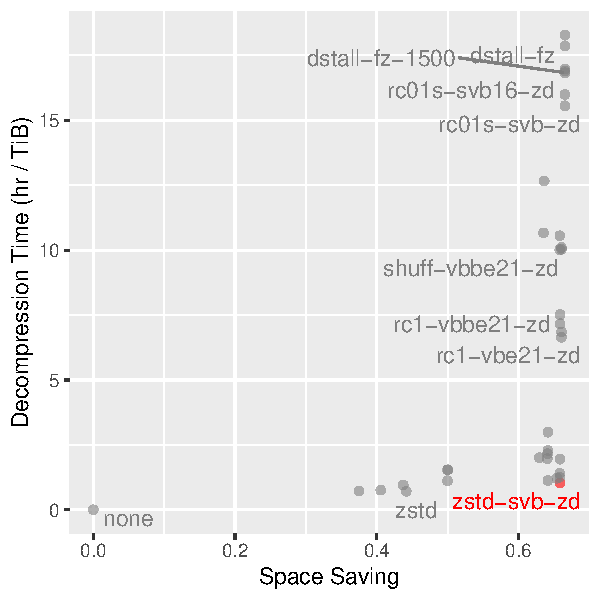
\includegraphics[scale=0.7,valign=t]{plots/reads.blow5.test.ss-dt.pdf}
}
\subfloat[\label{fig:results-ss-dt-small}]{
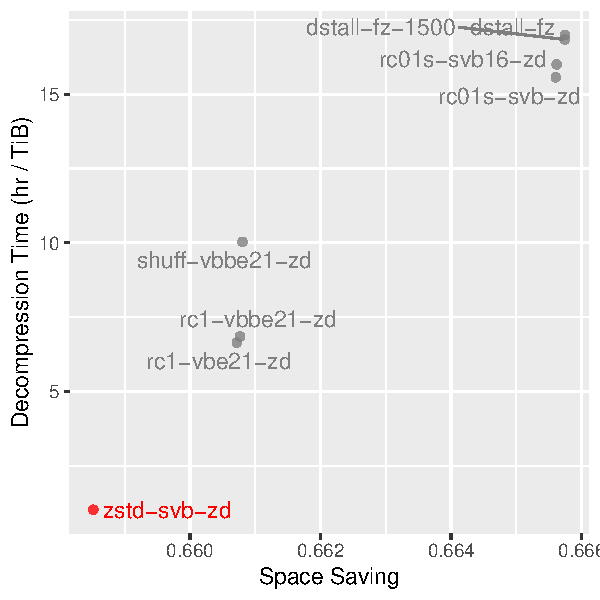
\includegraphics[scale=0.7,valign=t]{plots/reads.blow5.test.ss-dt06.pdf}
}
\caption{\label{fig:results-ss-t}The (de)compression time (in hours per TiB)
	versus space saving of various methods. The state-of-the-art method is
	coloured in red and the labelled methods are on the
	space--(de)compression-time frontier. That is, for each labelled method
	in Figures \ref{fig:results-ss-ct-big} and
	\ref{fig:results-ss-ct-small}
	there is no other compression method which produces a greater space
	saving in less time. Whilst for each labelled method in Figures
	\ref{fig:results-ss-dt-big} and \ref{fig:results-ss-dt-small} there is
	no other compression method which has a greater space saving and
	decompresses in less time.
	Figures \ref{fig:results-ss-ct-big} and \ref{fig:results-ss-dt-big} show all the
	methods. Whilst Figures \ref{fig:results-ss-ct-small} and
	\ref{fig:results-ss-dt-small} show the methods which are on their
	respective froniter and have a space saving greater than or equal to the
	state-of-the-art.}
\end{figure}

\begin{figure}
\centering
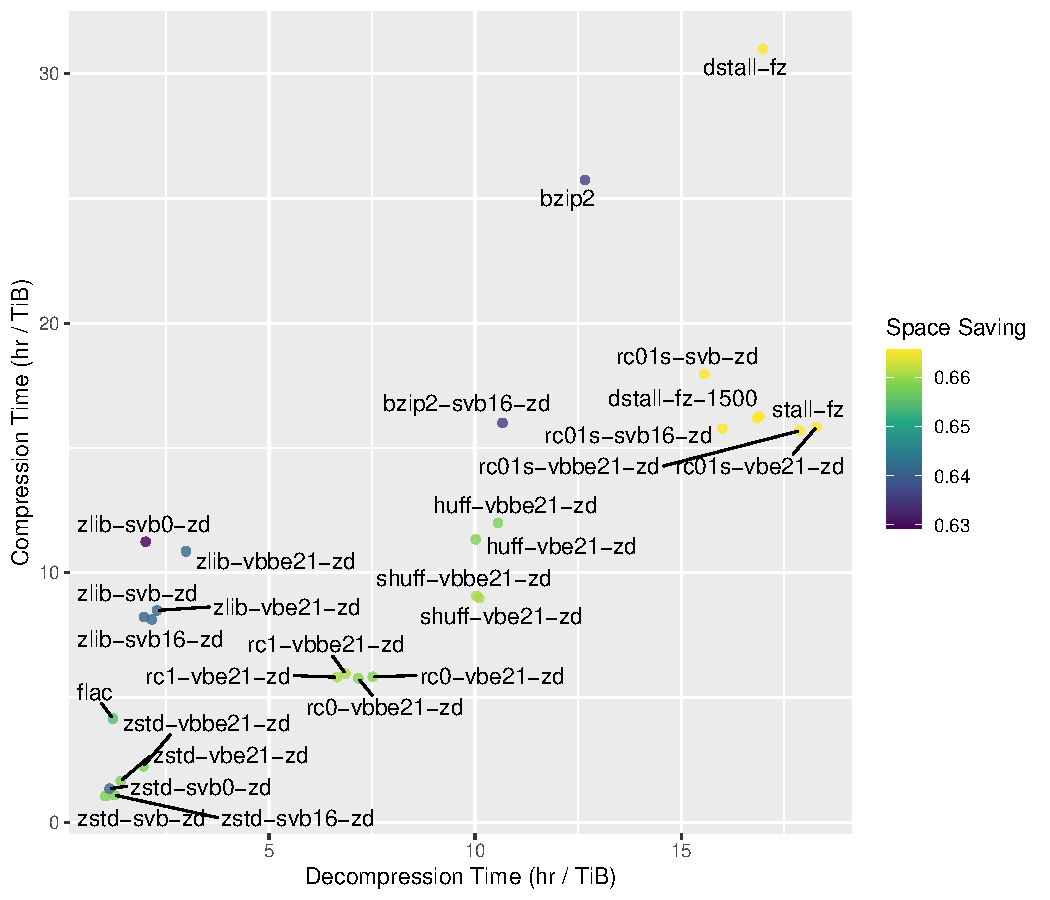
\includegraphics[scale=0.7]{plots/reads.blow5.test.ct-dt.pdf}
	\caption{\label{fig:results-ct-dt}A scatter plot of the methods which
	have a space saving greater than or equal to the state-of-the-art.
	Compression time is plotted against decompression time (in hours per
	TiB) and each point is coloured by its space saving. The
	state-of-the-art method zstd-svb-zd is in the bottom-left corner.}
\end{figure}


%\begin{table}
    \caption{\label{tab:vbz} Performance results on the data set using only one thread of execution.}
	\begin{tabular}{|l|l|}
        \hline
Compression Ratio & 2.93\\
		Compression Speed (mins per TiB) & 62.5\\

		Decompression Speed (mins per TiB) & 61.5\\
	\hline
    \end{tabular}
\end{table}


\chapter{Discussion} \label{chap:disc}

\section{Future Work}

Different length reads may have different characteristics which are exploitable for a compression algorithm.
Reads from the same pore or channel may have similar characteristics as well.

%Multi-read compression?
%Lossy
%Using metadata more
%Differential coding over larger distances

\chapter{Conclusion} \label{chap:conclusion}

Nanopore sequencing is a next-generation approach to DNA sequencing known for
its speed, portability, long reads and real-time analysis. Its increasing
popularity has been further influenced by the advent of the COVID-19 pandemic
which resulted in approximately one quarter of all SARS-CoV-2 virus genomes
being sequenced by nanopore devices \cite{lara}. This popularity has caused a
dramatic increase in data storage costs pertaining to the magnitude of the data
which is around 1 TB per human DNA sequencing run.
The current approach to compressing this data does not consider its
unique characteristics and thus misses crucial space saving opportunities.

As a result, we set out to discover lossless compression methods for archiving
nanopore signal data which achieve more space saving that the current
state-of-the-art.
Data compression is fundamentally an artificial intelligence problem of
understanding the data and making the correct predictions. Hence, after
providing the background material for the thesis, we conducted a systematic
analysis of the signal data including an examination of its characteristics and
suitable transformations.
Then, we explored several strategies which exploit the signal data's
characteristics including the vbbe21-zd encoding, static Huffman, optimal
subsequence searching, stall-specific encoding and separating the jumps and
falls from the flats.
After setting up the first comprehensive benchmark of existing and novel
compression methods for nanopore signal data, a large experiment was conducted
wherein each read from the downsampled NA12878 data set was compressed and
decompressed sequentially using each method.
Space and time metrics were collected and a superior space saving of 0.666
versus 0.659 -- which outperforms the entropy of the deltas -- was achieved
using the dstall-fz method. This strategy combines vbbe21 with dynamic stall
encoding and range coding modelled by order-0 order-1 SSE. Furthermore, an
alternative dynamic stall encoder, dstall-fz-1500, was found to approximate the
decision boundary of dstall-fz whilst achieving the same space saving of 0.666 in
half the compression time.

\chapter*{Appendix} \label{chap:appendix}

\section{Subsequence Searching}

%TODO sort this out better

Using the arithmetico-geometric series formula
\label{app:phi}
\begin{align*}
	\phi_n &= O(n) + 2\sum_{1\le k\le n-1}3^{k-1}O(n-k)\\
&= O(n) + 2\left(\frac{O(n-1) - 0}{1-3} - \frac{3}{(1-3)^2}(1-3^{n-1})\right)\\
&= O(n) - O(n-1) + \frac{3}{2}(3^{n-1}-1)\\
&= O(n) - O(n-1) + \frac{3^n}{2} - \frac{3}{2}
\end{align*}

\label{app:xi}
\begin{align*}
	\xi_n &= 2\times 3^{n-2}+\sum_{1\le k\le n-2}3^{k-1}(n-k)\\
	&= 2\times 3^{n-2} + \frac{(n-1)-3^{n-2}}{1-3}-\frac{3}{(1-3)^2}(1-3^{n-2})\\
	&= 2\times 3^{n-2} + \frac{3^{n-2}-n+1}{2}+\frac{3}{4}(3^{n-2}-1)\\
	&= 2\times 3^{n-2} + \frac{5}{4}\times 3^{n-2}-\frac{n-1}{2}-\frac{3}{4}\\
	&= 2\times 3^{n-2}+\frac{5}{4}\times 3^{n-2}-\frac{2n+1}{4}
\end{align*}



%%%%%%%%%%%%
% End

% Bibliography
\bibliographystyle{style/mybibstyle}
{
\setstretch{1.25}
\cleardoublepage
\phantomsection
\bibliography{references}
}

%%%% Appendices
%%%\appendix
%%%\addtocontents{toc}{\protect\setcounter{tocdepth}{1}}
%%%\input{wikifeats/wikifeats.tex}
%%%\input{candcner/candcner.tex}
%%%\input{comparedata/comparedata.tex}

\end{document}
